\documentclass[twoside]{book}

% Packages required by doxygen
\usepackage{fixltx2e}
\usepackage{calc}
\usepackage{doxygen}
\usepackage[export]{adjustbox} % also loads graphicx
\usepackage{graphicx}
\usepackage[utf8]{inputenc}
\usepackage{makeidx}
\usepackage{multicol}
\usepackage{multirow}
\PassOptionsToPackage{warn}{textcomp}
\usepackage{textcomp}
\usepackage[nointegrals]{wasysym}
\usepackage[table]{xcolor}

% Font selection
\usepackage[T1]{fontenc}
\usepackage[scaled=.90]{helvet}
\usepackage{courier}
\usepackage{amssymb}
\usepackage{sectsty}
\renewcommand{\familydefault}{\sfdefault}
\allsectionsfont{%
  \fontseries{bc}\selectfont%
  \color{darkgray}%
}
\renewcommand{\DoxyLabelFont}{%
  \fontseries{bc}\selectfont%
  \color{darkgray}%
}
\newcommand{\+}{\discretionary{\mbox{\scriptsize$\hookleftarrow$}}{}{}}

% Page & text layout
\usepackage{geometry}
\geometry{%
  a4paper,%
  top=2.5cm,%
  bottom=2.5cm,%
  left=2.5cm,%
  right=2.5cm%
}
\tolerance=750
\hfuzz=15pt
\hbadness=750
\setlength{\emergencystretch}{15pt}
\setlength{\parindent}{0cm}
\setlength{\parskip}{0.2cm}
\makeatletter
\renewcommand{\paragraph}{%
  \@startsection{paragraph}{4}{0ex}{-1.0ex}{1.0ex}{%
    \normalfont\normalsize\bfseries\SS@parafont%
  }%
}
\renewcommand{\subparagraph}{%
  \@startsection{subparagraph}{5}{0ex}{-1.0ex}{1.0ex}{%
    \normalfont\normalsize\bfseries\SS@subparafont%
  }%
}
\makeatother

% Headers & footers
\usepackage{fancyhdr}
\pagestyle{fancyplain}
\fancyhead[LE]{\fancyplain{}{\bfseries\thepage}}
\fancyhead[CE]{\fancyplain{}{}}
\fancyhead[RE]{\fancyplain{}{\bfseries\leftmark}}
\fancyhead[LO]{\fancyplain{}{\bfseries\rightmark}}
\fancyhead[CO]{\fancyplain{}{}}
\fancyhead[RO]{\fancyplain{}{\bfseries\thepage}}
\fancyfoot[LE]{\fancyplain{}{}}
\fancyfoot[CE]{\fancyplain{}{}}
\fancyfoot[RE]{\fancyplain{}{\bfseries\scriptsize Generated on Thu Jun 2 2016 23\+:06\+:11 for Destroyer2\+D by Doxygen }}
\fancyfoot[LO]{\fancyplain{}{\bfseries\scriptsize Generated on Thu Jun 2 2016 23\+:06\+:11 for Destroyer2\+D by Doxygen }}
\fancyfoot[CO]{\fancyplain{}{}}
\fancyfoot[RO]{\fancyplain{}{}}
\renewcommand{\footrulewidth}{0.4pt}
\renewcommand{\chaptermark}[1]{%
  \markboth{#1}{}%
}
\renewcommand{\sectionmark}[1]{%
  \markright{\thesection\ #1}%
}

% Indices & bibliography
\usepackage{natbib}
\usepackage[titles]{tocloft}
\setcounter{tocdepth}{3}
\setcounter{secnumdepth}{5}
\makeindex

% Hyperlinks (required, but should be loaded last)
\usepackage{ifpdf}
\ifpdf
  \usepackage[pdftex,pagebackref=true]{hyperref}
\else
  \usepackage[ps2pdf,pagebackref=true]{hyperref}
\fi
\hypersetup{%
  colorlinks=true,%
  linkcolor=blue,%
  citecolor=blue,%
  unicode%
}

% Custom commands
\newcommand{\clearemptydoublepage}{%
  \newpage{\pagestyle{empty}\cleardoublepage}%
}


%===== C O N T E N T S =====

\begin{document}

% Titlepage & ToC
\hypersetup{pageanchor=false,
             bookmarks=true,
             bookmarksnumbered=true,
             pdfencoding=unicode
            }
\pagenumbering{roman}
\begin{titlepage}
\vspace*{7cm}
\begin{center}%
{\Large Destroyer2\+D }\\
\vspace*{1cm}
{\large Generated by Doxygen 1.8.9.1}\\
\vspace*{0.5cm}
{\small Thu Jun 2 2016 23:06:11}\\
\end{center}
\end{titlepage}
\clearemptydoublepage
\tableofcontents
\clearemptydoublepage
\pagenumbering{arabic}
\hypersetup{pageanchor=true}

%--- Begin generated contents ---
\chapter{Hierarchical Index}
\section{Class Hierarchy}
This inheritance list is sorted roughly, but not completely, alphabetically\+:\begin{DoxyCompactList}
\item \contentsline{section}{Enemy\+:\+:action\+\_\+t}{\pageref{structEnemy_1_1action__t}}{}
\item b2\+Contact\+Listener\begin{DoxyCompactList}
\item \contentsline{section}{World\+:\+:My\+Contact\+Listener}{\pageref{classWorld_1_1MyContactListener}}{}
\end{DoxyCompactList}
\item b2\+Destruction\+Listener\begin{DoxyCompactList}
\item \contentsline{section}{Dragging\+Callback\+:\+:Local\+Listener}{\pageref{classDraggingCallback_1_1LocalListener}}{}
\item \contentsline{section}{World\+:\+:My\+Destruction\+Listener}{\pageref{classWorld_1_1MyDestructionListener}}{}
\end{DoxyCompactList}
\item b2\+Query\+Callback\begin{DoxyCompactList}
\item \contentsline{section}{World\+:\+:Global\+Test\+Point}{\pageref{classWorld_1_1GlobalTestPoint}}{}
\end{DoxyCompactList}
\item \contentsline{section}{Enemy}{\pageref{classEnemy}}{}
\item \contentsline{section}{Render\+:\+:Fixture\+Renderer}{\pageref{classRender_1_1FixtureRenderer}}{}
\begin{DoxyCompactList}
\item \contentsline{section}{Render\+:\+:Polygon\+Renderer}{\pageref{classRender_1_1PolygonRenderer}}{}
\end{DoxyCompactList}
\item \contentsline{section}{Matter}{\pageref{classMatter}}{}
\begin{DoxyCompactList}
\item \contentsline{section}{Particle\+System}{\pageref{classParticleSystem}}{}
\begin{DoxyCompactList}
\item \contentsline{section}{Dust}{\pageref{classDust}}{}
\item \contentsline{section}{Flame}{\pageref{classFlame}}{}
\item \contentsline{section}{Water\+Square}{\pageref{classWaterSquare}}{}
\end{DoxyCompactList}
\item \contentsline{section}{Rigid}{\pageref{classRigid}}{}
\begin{DoxyCompactList}
\item \contentsline{section}{Block}{\pageref{classBlock}}{}
\begin{DoxyCompactList}
\item \contentsline{section}{Engine}{\pageref{classEngine}}{}
\begin{DoxyCompactList}
\item \contentsline{section}{Large\+Engine}{\pageref{classLargeEngine}}{}
\item \contentsline{section}{Small\+Engine}{\pageref{classSmallEngine}}{}
\end{DoxyCompactList}
\item \contentsline{section}{Large\+Wood\+Block}{\pageref{classLargeWoodBlock}}{}
\item \contentsline{section}{Small\+Wood\+Block}{\pageref{classSmallWoodBlock}}{}
\end{DoxyCompactList}
\item \contentsline{section}{Bomb}{\pageref{classBomb}}{}
\item \contentsline{section}{Button$<$ image\+Name $>$}{\pageref{classButton}}{}
\item \contentsline{section}{Frame}{\pageref{classFrame}}{}
\item \contentsline{section}{Small\+Steel\+Ball}{\pageref{classSmallSteelBall}}{}
\item \contentsline{section}{Stick}{\pageref{classStick}}{}
\begin{DoxyCompactList}
\item \contentsline{section}{Steel\+Stick}{\pageref{classSteelStick}}{}
\item \contentsline{section}{Wood\+Stick}{\pageref{classWoodStick}}{}
\end{DoxyCompactList}
\end{DoxyCompactList}
\end{DoxyCompactList}
\item \contentsline{section}{Mouse\+Callback}{\pageref{classMouseCallback}}{}
\begin{DoxyCompactList}
\item \contentsline{section}{Cancel\+Callback}{\pageref{classCancelCallback}}{}
\item \contentsline{section}{Delete\+Button\+Callback}{\pageref{classDeleteButtonCallback}}{}
\item \contentsline{section}{Deleting\+Callback}{\pageref{classDeletingCallback}}{}
\item \contentsline{section}{Dragging\+Callback}{\pageref{classDraggingCallback}}{}
\item \contentsline{section}{Launch\+Callback}{\pageref{classLaunchCallback}}{}
\item \contentsline{section}{New\+Object\+Callback$<$ To\+Put $>$}{\pageref{classNewObjectCallback}}{}
\item \contentsline{section}{Putting\+Callback$<$ To\+Put $>$}{\pageref{classPuttingCallback}}{}
\item \contentsline{section}{Putting\+Line\+Callback$<$ To\+Put $>$}{\pageref{classPuttingLineCallback}}{}
\end{DoxyCompactList}
\item \contentsline{section}{Mouse\+Handler}{\pageref{classMouseHandler}}{}
\item \contentsline{section}{Render}{\pageref{classRender}}{}
\item \contentsline{section}{Saver}{\pageref{classSaver}}{}
\item \contentsline{section}{Window}{\pageref{classWindow}}{}
\item \contentsline{section}{World}{\pageref{classWorld}}{}
\begin{DoxyCompactList}
\item \contentsline{section}{Main\+World}{\pageref{classMainWorld}}{}
\end{DoxyCompactList}
\end{DoxyCompactList}

\chapter{Class Index}
\section{Class List}
Here are the classes, structs, unions and interfaces with brief descriptions\+:\begin{DoxyCompactList}
\item\contentsline{section}{\hyperlink{structEnemy_1_1action__t}{Enemy\+::action\+\_\+t} }{\pageref{structEnemy_1_1action__t}}{}
\item\contentsline{section}{\hyperlink{classBlock}{Block} \\*Base class of all dynamic square rigids }{\pageref{classBlock}}{}
\item\contentsline{section}{\hyperlink{classBomb}{Bomb} \\*R=0.\+5 round bomb }{\pageref{classBomb}}{}
\item\contentsline{section}{\hyperlink{classButton}{Button$<$ image\+Name $>$} }{\pageref{classButton}}{}
\item\contentsline{section}{\hyperlink{classCancelCallback}{Cancel\+Callback} }{\pageref{classCancelCallback}}{}
\item\contentsline{section}{\hyperlink{classDeleteButtonCallback}{Delete\+Button\+Callback} }{\pageref{classDeleteButtonCallback}}{}
\item\contentsline{section}{\hyperlink{classDeletingCallback}{Deleting\+Callback} }{\pageref{classDeletingCallback}}{}
\item\contentsline{section}{\hyperlink{classDraggingCallback}{Dragging\+Callback} }{\pageref{classDraggingCallback}}{}
\item\contentsline{section}{\hyperlink{classDust}{Dust} \\*\hyperlink{classDust}{Dust} rised when a rigid is damaged }{\pageref{classDust}}{}
\item\contentsline{section}{\hyperlink{classEnemy}{Enemy} \\*This class loads and controls enemy }{\pageref{classEnemy}}{}
\item\contentsline{section}{\hyperlink{classEngine}{Engine} \\*Base class of engines }{\pageref{classEngine}}{}
\item\contentsline{section}{\hyperlink{classRender_1_1FixtureRenderer}{Render\+::\+Fixture\+Renderer} }{\pageref{classRender_1_1FixtureRenderer}}{}
\item\contentsline{section}{\hyperlink{classFlame}{Flame} \\*Set when bomb exploses }{\pageref{classFlame}}{}
\item\contentsline{section}{\hyperlink{classFrame}{Frame} \\*\hyperlink{classFrame}{Frame} around the world 1 unit thick }{\pageref{classFrame}}{}
\item\contentsline{section}{\hyperlink{classWorld_1_1GlobalTestPoint}{World\+::\+Global\+Test\+Point} \\*A helper for finding a fixture overlapping with a point }{\pageref{classWorld_1_1GlobalTestPoint}}{}
\item\contentsline{section}{\hyperlink{classLargeEngine}{Large\+Engine} \\*2\+X4 Large engine that will provide a 300\+N force }{\pageref{classLargeEngine}}{}
\item\contentsline{section}{\hyperlink{classLargeWoodBlock}{Large\+Wood\+Block} \\*Dynamic 3\+X3 large wooden block Will Float }{\pageref{classLargeWoodBlock}}{}
\item\contentsline{section}{\hyperlink{classLaunchCallback}{Launch\+Callback} }{\pageref{classLaunchCallback}}{}
\item\contentsline{section}{\hyperlink{classDraggingCallback_1_1LocalListener}{Dragging\+Callback\+::\+Local\+Listener} }{\pageref{classDraggingCallback_1_1LocalListener}}{}
\item\contentsline{section}{\hyperlink{classMainWorld}{Main\+World} \\*This world is the main scenery of the game }{\pageref{classMainWorld}}{}
\item\contentsline{section}{\hyperlink{classMatter}{Matter} \\*Base class of all rigid bodies and particles }{\pageref{classMatter}}{}
\item\contentsline{section}{\hyperlink{classMouseCallback}{Mouse\+Callback} \\*This file consists of template classes of mouse callback listeners }{\pageref{classMouseCallback}}{}
\item\contentsline{section}{\hyperlink{classMouseHandler}{Mouse\+Handler} \\*Forwards mouse actions to \hyperlink{classMatter}{Matter} }{\pageref{classMouseHandler}}{}
\item\contentsline{section}{\hyperlink{classWorld_1_1MyContactListener}{World\+::\+My\+Contact\+Listener} }{\pageref{classWorld_1_1MyContactListener}}{}
\item\contentsline{section}{\hyperlink{classWorld_1_1MyDestructionListener}{World\+::\+My\+Destruction\+Listener} \\*Manger for all destruction listener }{\pageref{classWorld_1_1MyDestructionListener}}{}
\item\contentsline{section}{\hyperlink{classNewObjectCallback}{New\+Object\+Callback$<$ To\+Put $>$} }{\pageref{classNewObjectCallback}}{}
\item\contentsline{section}{\hyperlink{classParticleSystem}{Particle\+System} \\*Base class of all particle systems }{\pageref{classParticleSystem}}{}
\item\contentsline{section}{\hyperlink{classRender_1_1PolygonRenderer}{Render\+::\+Polygon\+Renderer} }{\pageref{classRender_1_1PolygonRenderer}}{}
\item\contentsline{section}{\hyperlink{classPuttingCallback}{Putting\+Callback$<$ To\+Put $>$} \\*Callbacks of putting normal things that ! can\+Draw\+Line() }{\pageref{classPuttingCallback}}{}
\item\contentsline{section}{\hyperlink{classPuttingLineCallback}{Putting\+Line\+Callback$<$ To\+Put $>$} \\*Putting rigids with can\+Draw\+Line() }{\pageref{classPuttingLineCallback}}{}
\item\contentsline{section}{\hyperlink{classRender}{Render} }{\pageref{classRender}}{}
\item\contentsline{section}{\hyperlink{classRigid}{Rigid} \\*Base class of all rigid bodies }{\pageref{classRigid}}{}
\item\contentsline{section}{\hyperlink{classSaver}{Saver} \\*\hyperlink{classSaver}{Saver} manages game saving and loading }{\pageref{classSaver}}{}
\item\contentsline{section}{\hyperlink{classSmallEngine}{Small\+Engine} \\*1\+X2 Small engine that will provide a 30\+N force }{\pageref{classSmallEngine}}{}
\item\contentsline{section}{\hyperlink{classSmallSteelBall}{Small\+Steel\+Ball} \\*Steel r=0.\+5 ball }{\pageref{classSmallSteelBall}}{}
\item\contentsline{section}{\hyperlink{classSmallWoodBlock}{Small\+Wood\+Block} \\*Dynamic 1\+X1 small wooden block Will Float }{\pageref{classSmallWoodBlock}}{}
\item\contentsline{section}{\hyperlink{classSteelStick}{Steel\+Stick} }{\pageref{classSteelStick}}{}
\item\contentsline{section}{\hyperlink{classStick}{Stick} \\*Base class with all that \hyperlink{classStick_ad2b8a92274aed6d25d79c8b4033b2bfb}{can\+Draw\+Line()} Will create contact to what is linked }{\pageref{classStick}}{}
\item\contentsline{section}{\hyperlink{classWaterSquare}{Water\+Square} \\*A square water area This must be use as a pool where the number of particles is static }{\pageref{classWaterSquare}}{}
\item\contentsline{section}{\hyperlink{classWindow}{Window} \\*This class interact with G\+L\+F\+W }{\pageref{classWindow}}{}
\item\contentsline{section}{\hyperlink{classWoodStick}{Wood\+Stick} }{\pageref{classWoodStick}}{}
\item\contentsline{section}{\hyperlink{classWorld}{World} \\*All object in a scenario Interact with Open\+G\+L and Liquid\+Fun }{\pageref{classWorld}}{}
\end{DoxyCompactList}

\chapter{File Index}
\section{File List}
Here is a list of all files with brief descriptions\+:\begin{DoxyCompactList}
\item\contentsline{section}{\hyperlink{_8ycm__extra__conf_8py}{.\+ycm\+\_\+extra\+\_\+conf.\+py} }{\pageref{_8ycm__extra__conf_8py}}{}
\item\contentsline{section}{\hyperlink{const_8h}{const.\+h} }{\pageref{const_8h}}{}
\item\contentsline{section}{\hyperlink{enemy_8cpp}{enemy.\+cpp} }{\pageref{enemy_8cpp}}{}
\item\contentsline{section}{\hyperlink{enemy_8h}{enemy.\+h} }{\pageref{enemy_8h}}{}
\item\contentsline{section}{\hyperlink{image_8h}{image.\+h} }{\pageref{image_8h}}{}
\item\contentsline{section}{\hyperlink{loader_8cpp}{loader.\+cpp} }{\pageref{loader_8cpp}}{}
\item\contentsline{section}{\hyperlink{loader_8h}{loader.\+h} }{\pageref{loader_8h}}{}
\item\contentsline{section}{\hyperlink{main_8cpp}{main.\+cpp} }{\pageref{main_8cpp}}{}
\item\contentsline{section}{\hyperlink{matter_8cpp}{matter.\+cpp} }{\pageref{matter_8cpp}}{}
\item\contentsline{section}{\hyperlink{matter_8h}{matter.\+h} }{\pageref{matter_8h}}{}
\item\contentsline{section}{\hyperlink{mousecallback_8h}{mousecallback.\+h} }{\pageref{mousecallback_8h}}{}
\item\contentsline{section}{\hyperlink{mousehandler_8cpp}{mousehandler.\+cpp} }{\pageref{mousehandler_8cpp}}{}
\item\contentsline{section}{\hyperlink{mousehandler_8h}{mousehandler.\+h} }{\pageref{mousehandler_8h}}{}
\item\contentsline{section}{\hyperlink{render_8cpp}{render.\+cpp} }{\pageref{render_8cpp}}{}
\item\contentsline{section}{\hyperlink{render_8h}{render.\+h} }{\pageref{render_8h}}{}
\item\contentsline{section}{\hyperlink{saver_8cpp}{saver.\+cpp} }{\pageref{saver_8cpp}}{}
\item\contentsline{section}{\hyperlink{saver_8h}{saver.\+h} }{\pageref{saver_8h}}{}
\item\contentsline{section}{\hyperlink{window_8cpp}{window.\+cpp} }{\pageref{window_8cpp}}{}
\item\contentsline{section}{\hyperlink{window_8h}{window.\+h} }{\pageref{window_8h}}{}
\item\contentsline{section}{\hyperlink{world_8cpp}{world.\+cpp} }{\pageref{world_8cpp}}{}
\item\contentsline{section}{\hyperlink{world_8h}{world.\+h} }{\pageref{world_8h}}{}
\end{DoxyCompactList}

\chapter{Class Documentation}
\hypertarget{structEnemy_1_1action__t}{}\section{Enemy\+:\+:action\+\_\+t Struct Reference}
\label{structEnemy_1_1action__t}\index{Enemy\+::action\+\_\+t@{Enemy\+::action\+\_\+t}}


Collaboration diagram for Enemy\+:\+:action\+\_\+t\+:
\nopagebreak
\begin{figure}[H]
\begin{center}
\leavevmode
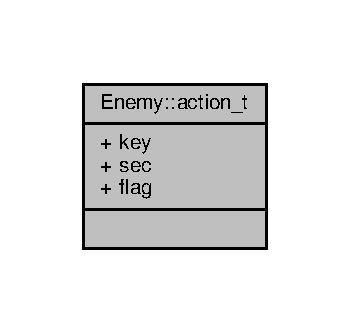
\includegraphics[width=168pt]{structEnemy_1_1action__t__coll__graph}
\end{center}
\end{figure}
\subsection*{Public Types}
\begin{DoxyCompactItemize}
\item 
enum \{ \hyperlink{structEnemy_1_1action__t_ab643a5e1949db5ccb006773412a9c12ba8786ddb5e8d54dfae1e13ae70adc113f}{P\+R\+E\+S\+S} = 0, 
\hyperlink{structEnemy_1_1action__t_ab643a5e1949db5ccb006773412a9c12ba4b7d9521cd8ba7262f1576b428580f78}{R\+E\+L\+E\+A\+S\+E} = 1
 \}
\end{DoxyCompactItemize}
\subsection*{Public Attributes}
\begin{DoxyCompactItemize}
\item 
char \hyperlink{structEnemy_1_1action__t_a107762072964a000ee4185e562d5f583}{key}
\item 
float \hyperlink{structEnemy_1_1action__t_a6098f9876645d5c23c656de57b51e24d}{sec}
\item 
int \hyperlink{structEnemy_1_1action__t_aea2f6b58cefc18ce0537e216cee3e96e}{flag}
\end{DoxyCompactItemize}


\subsection{Member Enumeration Documentation}
\hypertarget{structEnemy_1_1action__t_ab643a5e1949db5ccb006773412a9c12b}{}\subsubsection[{anonymous enum}]{\setlength{\rightskip}{0pt plus 5cm}anonymous enum}\label{structEnemy_1_1action__t_ab643a5e1949db5ccb006773412a9c12b}
\begin{Desc}
\item[Enumerator]\par
\begin{description}
\index{P\+R\+E\+S\+S@{P\+R\+E\+S\+S}!Enemy\+::action\+\_\+t@{Enemy\+::action\+\_\+t}}\index{Enemy\+::action\+\_\+t@{Enemy\+::action\+\_\+t}!P\+R\+E\+S\+S@{P\+R\+E\+S\+S}}\item[{\em 
\hypertarget{structEnemy_1_1action__t_ab643a5e1949db5ccb006773412a9c12ba8786ddb5e8d54dfae1e13ae70adc113f}{}P\+R\+E\+S\+S\label{structEnemy_1_1action__t_ab643a5e1949db5ccb006773412a9c12ba8786ddb5e8d54dfae1e13ae70adc113f}
}]\index{R\+E\+L\+E\+A\+S\+E@{R\+E\+L\+E\+A\+S\+E}!Enemy\+::action\+\_\+t@{Enemy\+::action\+\_\+t}}\index{Enemy\+::action\+\_\+t@{Enemy\+::action\+\_\+t}!R\+E\+L\+E\+A\+S\+E@{R\+E\+L\+E\+A\+S\+E}}\item[{\em 
\hypertarget{structEnemy_1_1action__t_ab643a5e1949db5ccb006773412a9c12ba4b7d9521cd8ba7262f1576b428580f78}{}R\+E\+L\+E\+A\+S\+E\label{structEnemy_1_1action__t_ab643a5e1949db5ccb006773412a9c12ba4b7d9521cd8ba7262f1576b428580f78}
}]\end{description}
\end{Desc}


\subsection{Member Data Documentation}
\hypertarget{structEnemy_1_1action__t_aea2f6b58cefc18ce0537e216cee3e96e}{}\index{Enemy\+::action\+\_\+t@{Enemy\+::action\+\_\+t}!flag@{flag}}
\index{flag@{flag}!Enemy\+::action\+\_\+t@{Enemy\+::action\+\_\+t}}
\subsubsection[{flag}]{\setlength{\rightskip}{0pt plus 5cm}int Enemy\+::action\+\_\+t\+::flag}\label{structEnemy_1_1action__t_aea2f6b58cefc18ce0537e216cee3e96e}
\hypertarget{structEnemy_1_1action__t_a107762072964a000ee4185e562d5f583}{}\index{Enemy\+::action\+\_\+t@{Enemy\+::action\+\_\+t}!key@{key}}
\index{key@{key}!Enemy\+::action\+\_\+t@{Enemy\+::action\+\_\+t}}
\subsubsection[{key}]{\setlength{\rightskip}{0pt plus 5cm}char Enemy\+::action\+\_\+t\+::key}\label{structEnemy_1_1action__t_a107762072964a000ee4185e562d5f583}
\hypertarget{structEnemy_1_1action__t_a6098f9876645d5c23c656de57b51e24d}{}\index{Enemy\+::action\+\_\+t@{Enemy\+::action\+\_\+t}!sec@{sec}}
\index{sec@{sec}!Enemy\+::action\+\_\+t@{Enemy\+::action\+\_\+t}}
\subsubsection[{sec}]{\setlength{\rightskip}{0pt plus 5cm}float Enemy\+::action\+\_\+t\+::sec}\label{structEnemy_1_1action__t_a6098f9876645d5c23c656de57b51e24d}


The documentation for this struct was generated from the following file\+:\begin{DoxyCompactItemize}
\item 
\hyperlink{enemy_8h}{enemy.\+h}\end{DoxyCompactItemize}

\hypertarget{classBlock}{}\section{Block Class Reference}
\label{classBlock}\index{Block@{Block}}


Base class of all dynamic square rigids.  




{\ttfamily \#include $<$matter.\+h$>$}



Inheritance diagram for Block\+:
\nopagebreak
\begin{figure}[H]
\begin{center}
\leavevmode
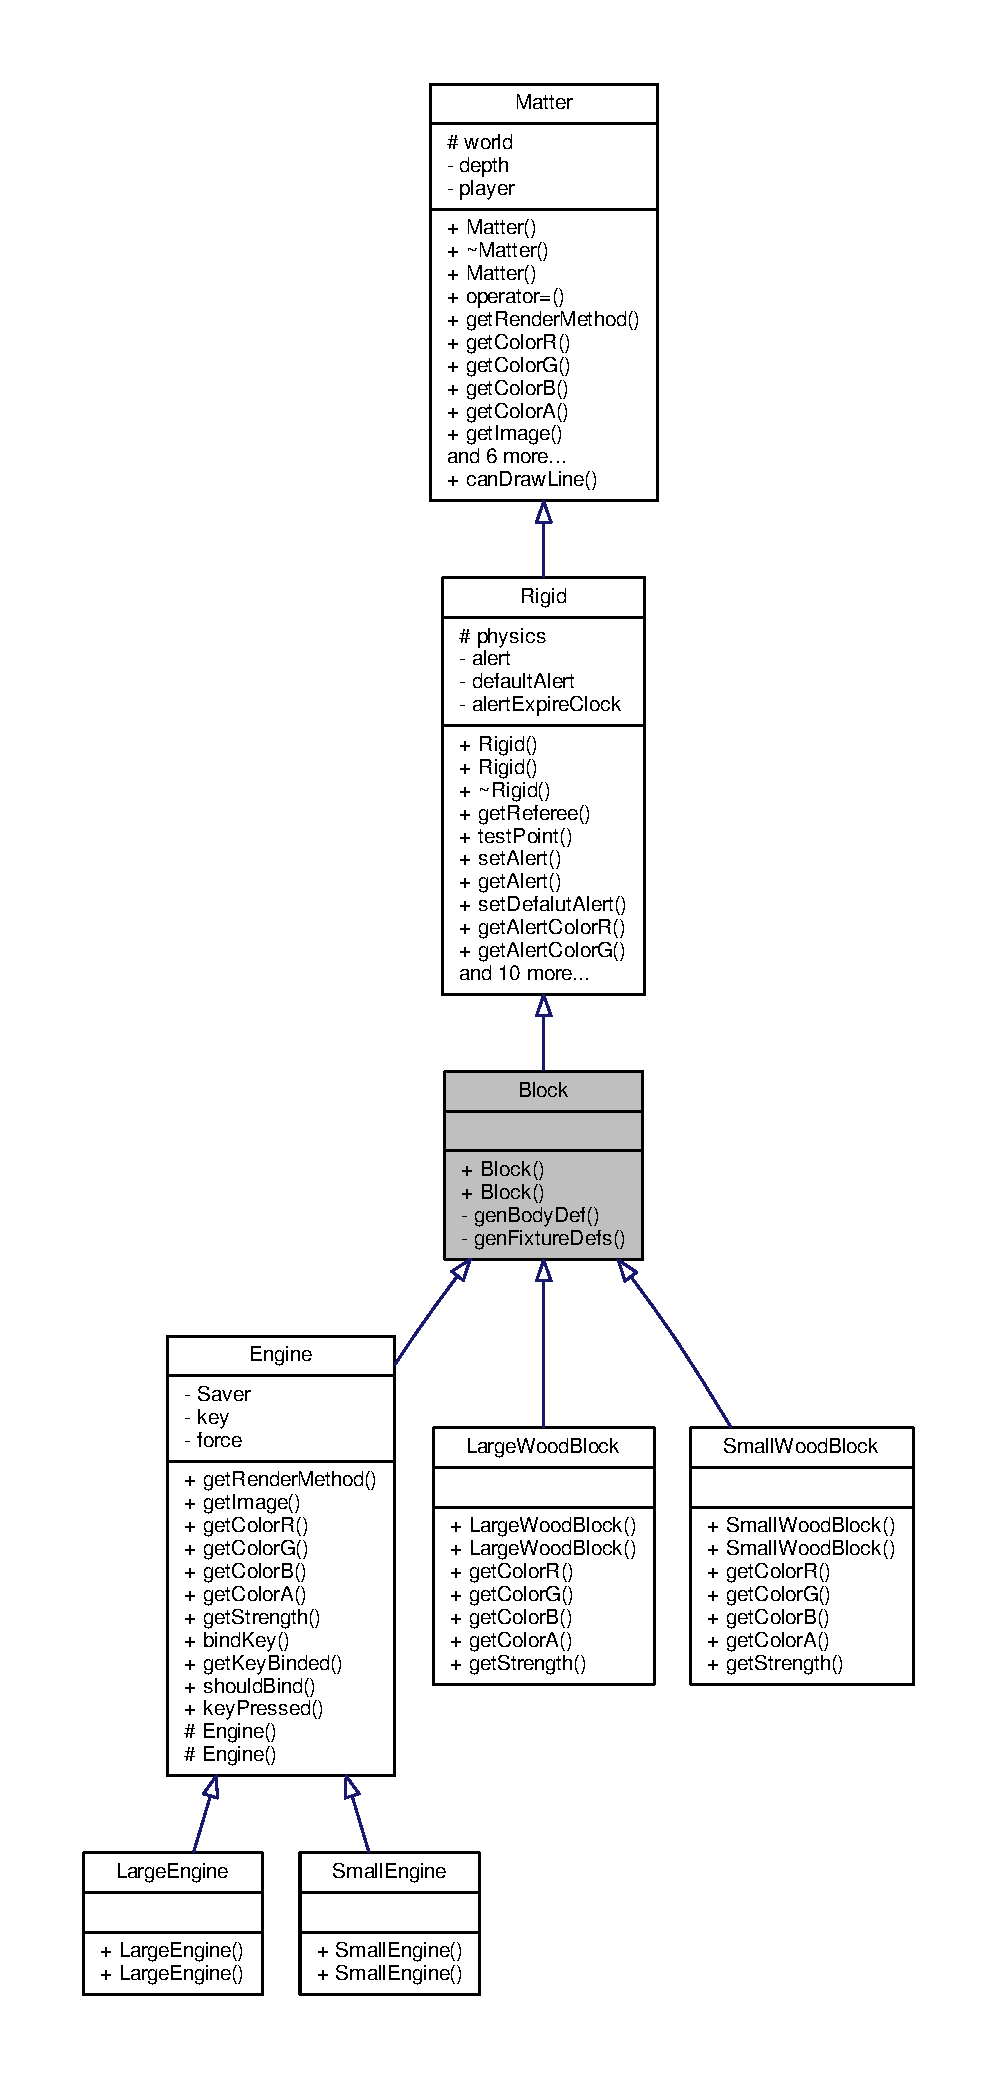
\includegraphics[height=550pt]{classBlock__inherit__graph}
\end{center}
\end{figure}


Collaboration diagram for Block\+:
\nopagebreak
\begin{figure}[H]
\begin{center}
\leavevmode
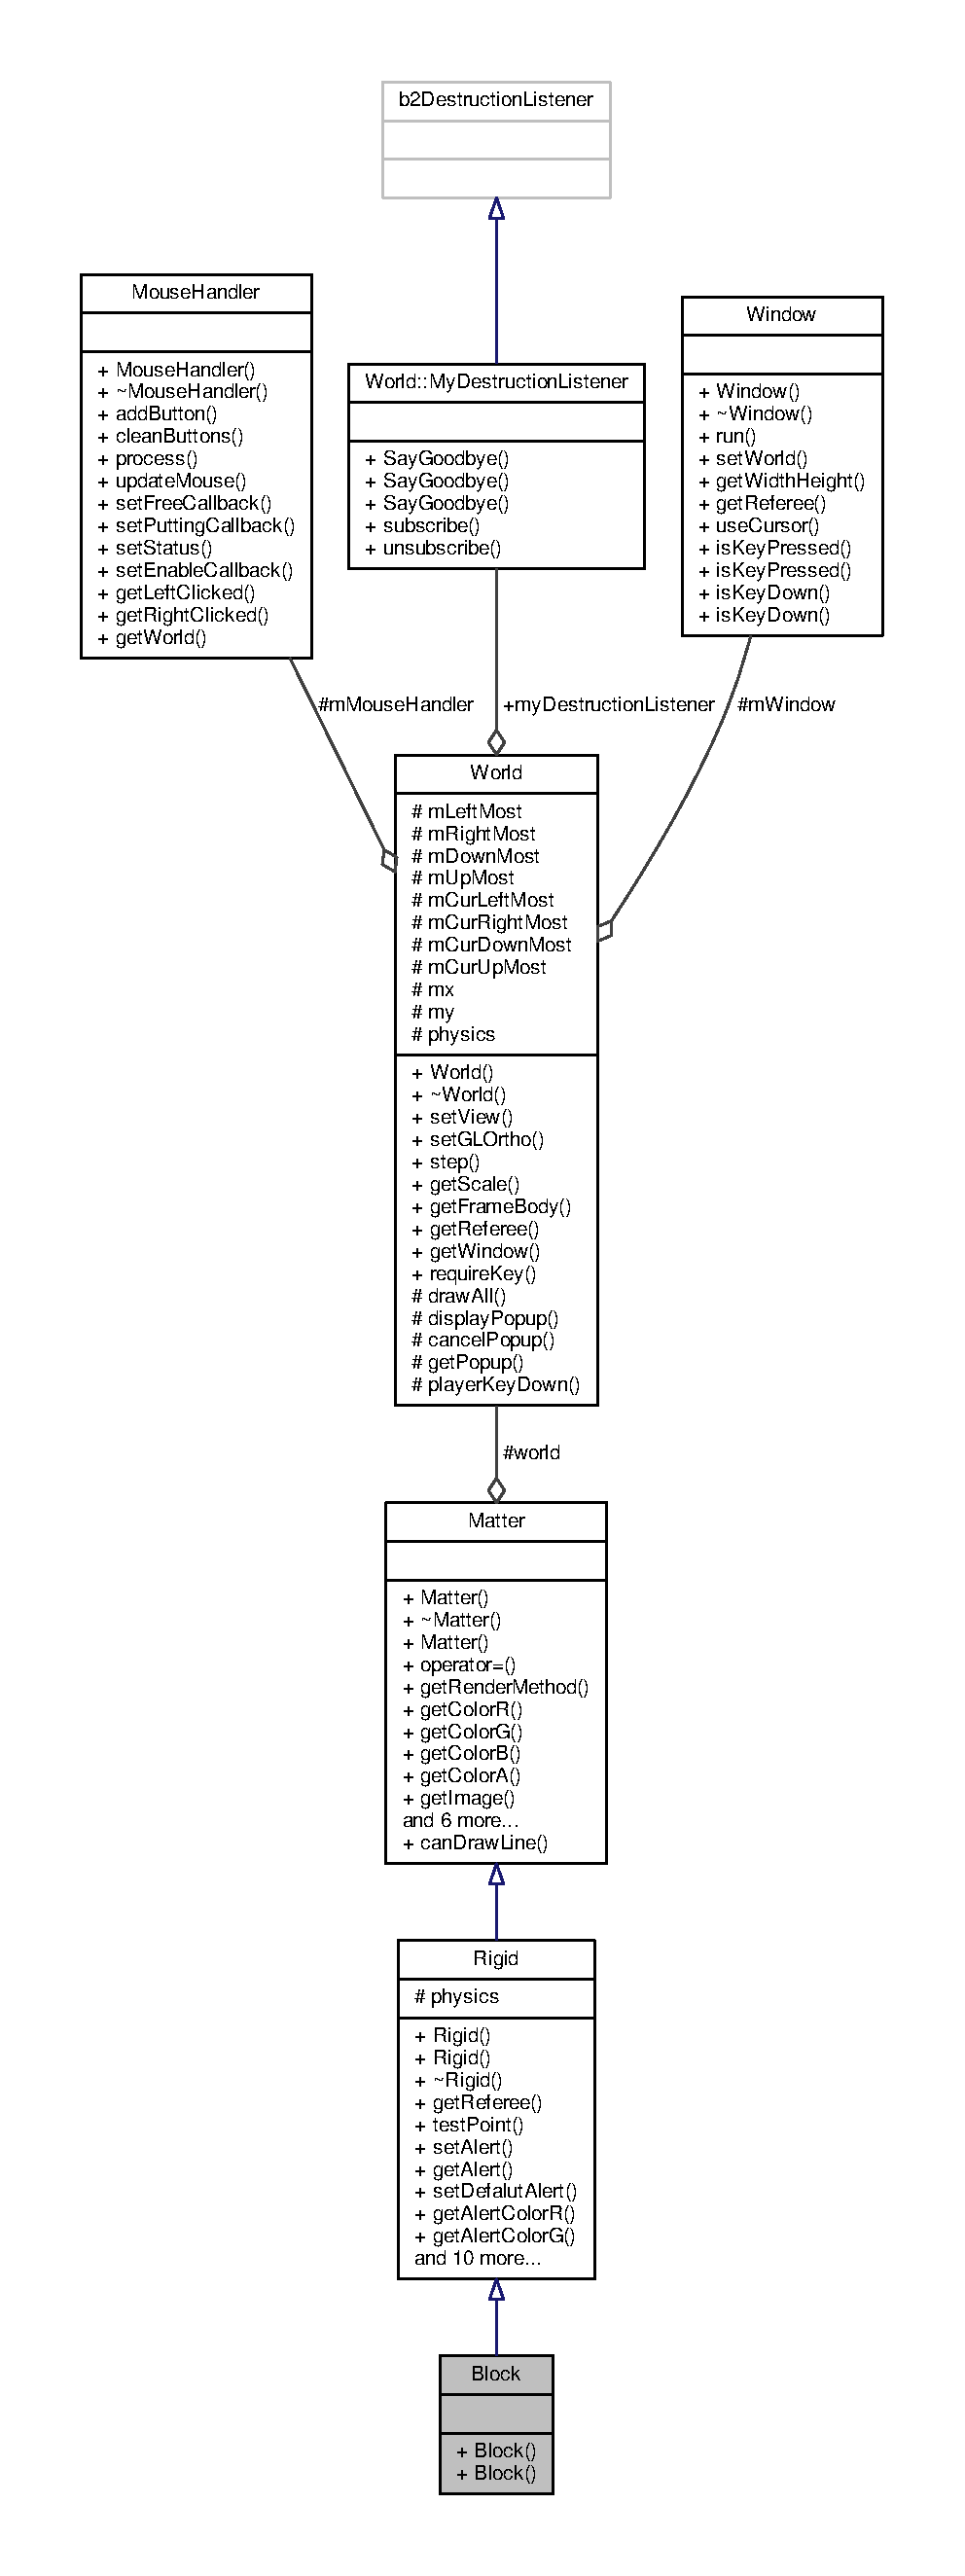
\includegraphics[height=550pt]{classBlock__coll__graph}
\end{center}
\end{figure}
\subsection*{Public Member Functions}
\begin{DoxyCompactItemize}
\item 
\hyperlink{classBlock_aae3e29e7e018dd11531c7ac7acbcc4b6}{Block} (\hyperlink{classWorld}{World} $\ast$\+\_\+world, b2\+Body $\ast$\hyperlink{image_8h_ab2d05693952610f937e5acb3c4a8fa1b}{b})
\item 
\hyperlink{classBlock_a2a61e69a3b1e77cb87fbd00da334b030}{Block} (\hyperlink{classWorld}{World} $\ast$\+\_\+world, float x, float y, float w, float h, float density, float friction, float restitution) noexcept
\end{DoxyCompactItemize}
\subsection*{Static Private Member Functions}
\begin{DoxyCompactItemize}
\item 
static b2\+Body\+Def \hyperlink{classBlock_a1510615e7ec7b95bc46fd33042fe315a}{gen\+Body\+Def} (float x, float y)
\item 
static std\+::vector$<$ b2\+Fixture\+Def $>$ \hyperlink{classBlock_a9ab5f250c9fc5f2de521bdecb3181ede}{gen\+Fixture\+Defs} (float w, float h, float density, float friction, float restitution)
\end{DoxyCompactItemize}
\subsection*{Additional Inherited Members}


\subsection{Detailed Description}
Base class of all dynamic square rigids. 

\subsection{Constructor \& Destructor Documentation}
\hypertarget{classBlock_aae3e29e7e018dd11531c7ac7acbcc4b6}{}\index{Block@{Block}!Block@{Block}}
\index{Block@{Block}!Block@{Block}}
\subsubsection[{Block}]{\setlength{\rightskip}{0pt plus 5cm}Block\+::\+Block (
\begin{DoxyParamCaption}
\item[{{\bf World} $\ast$}]{\+\_\+world, }
\item[{b2\+Body $\ast$}]{b}
\end{DoxyParamCaption}
)\hspace{0.3cm}{\ttfamily [inline]}}\label{classBlock_aae3e29e7e018dd11531c7ac7acbcc4b6}
\hypertarget{classBlock_a2a61e69a3b1e77cb87fbd00da334b030}{}\index{Block@{Block}!Block@{Block}}
\index{Block@{Block}!Block@{Block}}
\subsubsection[{Block}]{\setlength{\rightskip}{0pt plus 5cm}Block\+::\+Block (
\begin{DoxyParamCaption}
\item[{{\bf World} $\ast$}]{\+\_\+world, }
\item[{float}]{x, }
\item[{float}]{y, }
\item[{float}]{w, }
\item[{float}]{h, }
\item[{float}]{density, }
\item[{float}]{friction, }
\item[{float}]{restitution}
\end{DoxyParamCaption}
)\hspace{0.3cm}{\ttfamily [noexcept]}}\label{classBlock_a2a61e69a3b1e77cb87fbd00da334b030}


\subsection{Member Function Documentation}
\hypertarget{classBlock_a1510615e7ec7b95bc46fd33042fe315a}{}\index{Block@{Block}!gen\+Body\+Def@{gen\+Body\+Def}}
\index{gen\+Body\+Def@{gen\+Body\+Def}!Block@{Block}}
\subsubsection[{gen\+Body\+Def}]{\setlength{\rightskip}{0pt plus 5cm}b2\+Body\+Def Block\+::gen\+Body\+Def (
\begin{DoxyParamCaption}
\item[{float}]{x, }
\item[{float}]{y}
\end{DoxyParamCaption}
)\hspace{0.3cm}{\ttfamily [static]}, {\ttfamily [private]}}\label{classBlock_a1510615e7ec7b95bc46fd33042fe315a}
\hypertarget{classBlock_a9ab5f250c9fc5f2de521bdecb3181ede}{}\index{Block@{Block}!gen\+Fixture\+Defs@{gen\+Fixture\+Defs}}
\index{gen\+Fixture\+Defs@{gen\+Fixture\+Defs}!Block@{Block}}
\subsubsection[{gen\+Fixture\+Defs}]{\setlength{\rightskip}{0pt plus 5cm}std\+::vector$<$ b2\+Fixture\+Def $>$ Block\+::gen\+Fixture\+Defs (
\begin{DoxyParamCaption}
\item[{float}]{w, }
\item[{float}]{h, }
\item[{float}]{density, }
\item[{float}]{friction, }
\item[{float}]{restitution}
\end{DoxyParamCaption}
)\hspace{0.3cm}{\ttfamily [static]}, {\ttfamily [private]}}\label{classBlock_a9ab5f250c9fc5f2de521bdecb3181ede}


The documentation for this class was generated from the following files\+:\begin{DoxyCompactItemize}
\item 
\hyperlink{matter_8h}{matter.\+h}\item 
\hyperlink{matter_8cpp}{matter.\+cpp}\end{DoxyCompactItemize}

\hypertarget{classBomb}{}\section{Bomb Class Reference}
\label{classBomb}\index{Bomb@{Bomb}}


r=0.\+5 round bomb  




{\ttfamily \#include $<$matter.\+h$>$}



Inheritance diagram for Bomb\+:\nopagebreak
\begin{figure}[H]
\begin{center}
\leavevmode
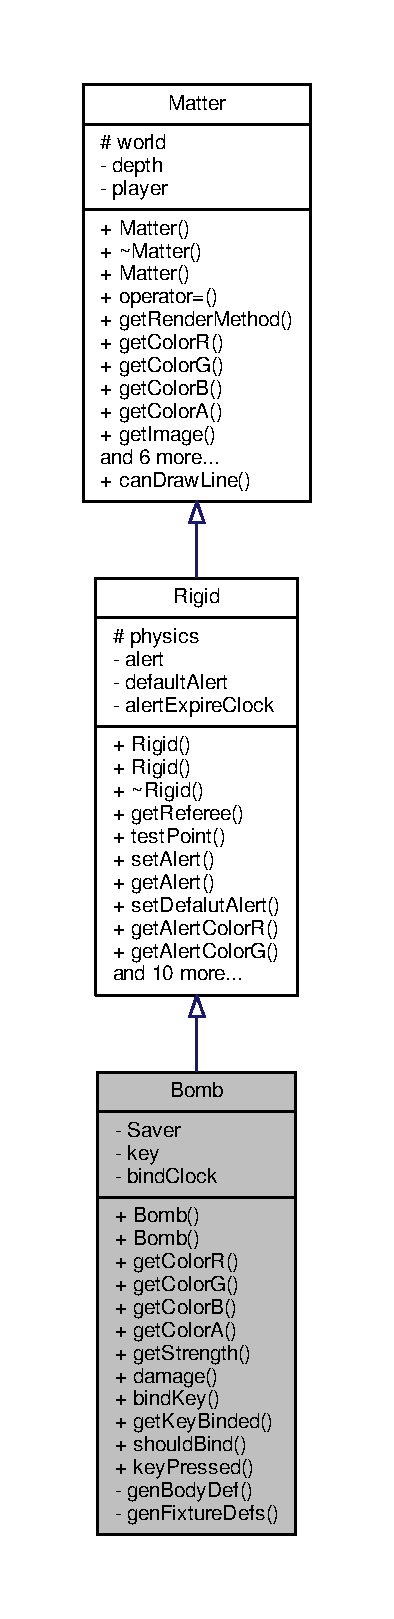
\includegraphics[height=550pt]{classBomb__inherit__graph}
\end{center}
\end{figure}


Collaboration diagram for Bomb\+:\nopagebreak
\begin{figure}[H]
\begin{center}
\leavevmode
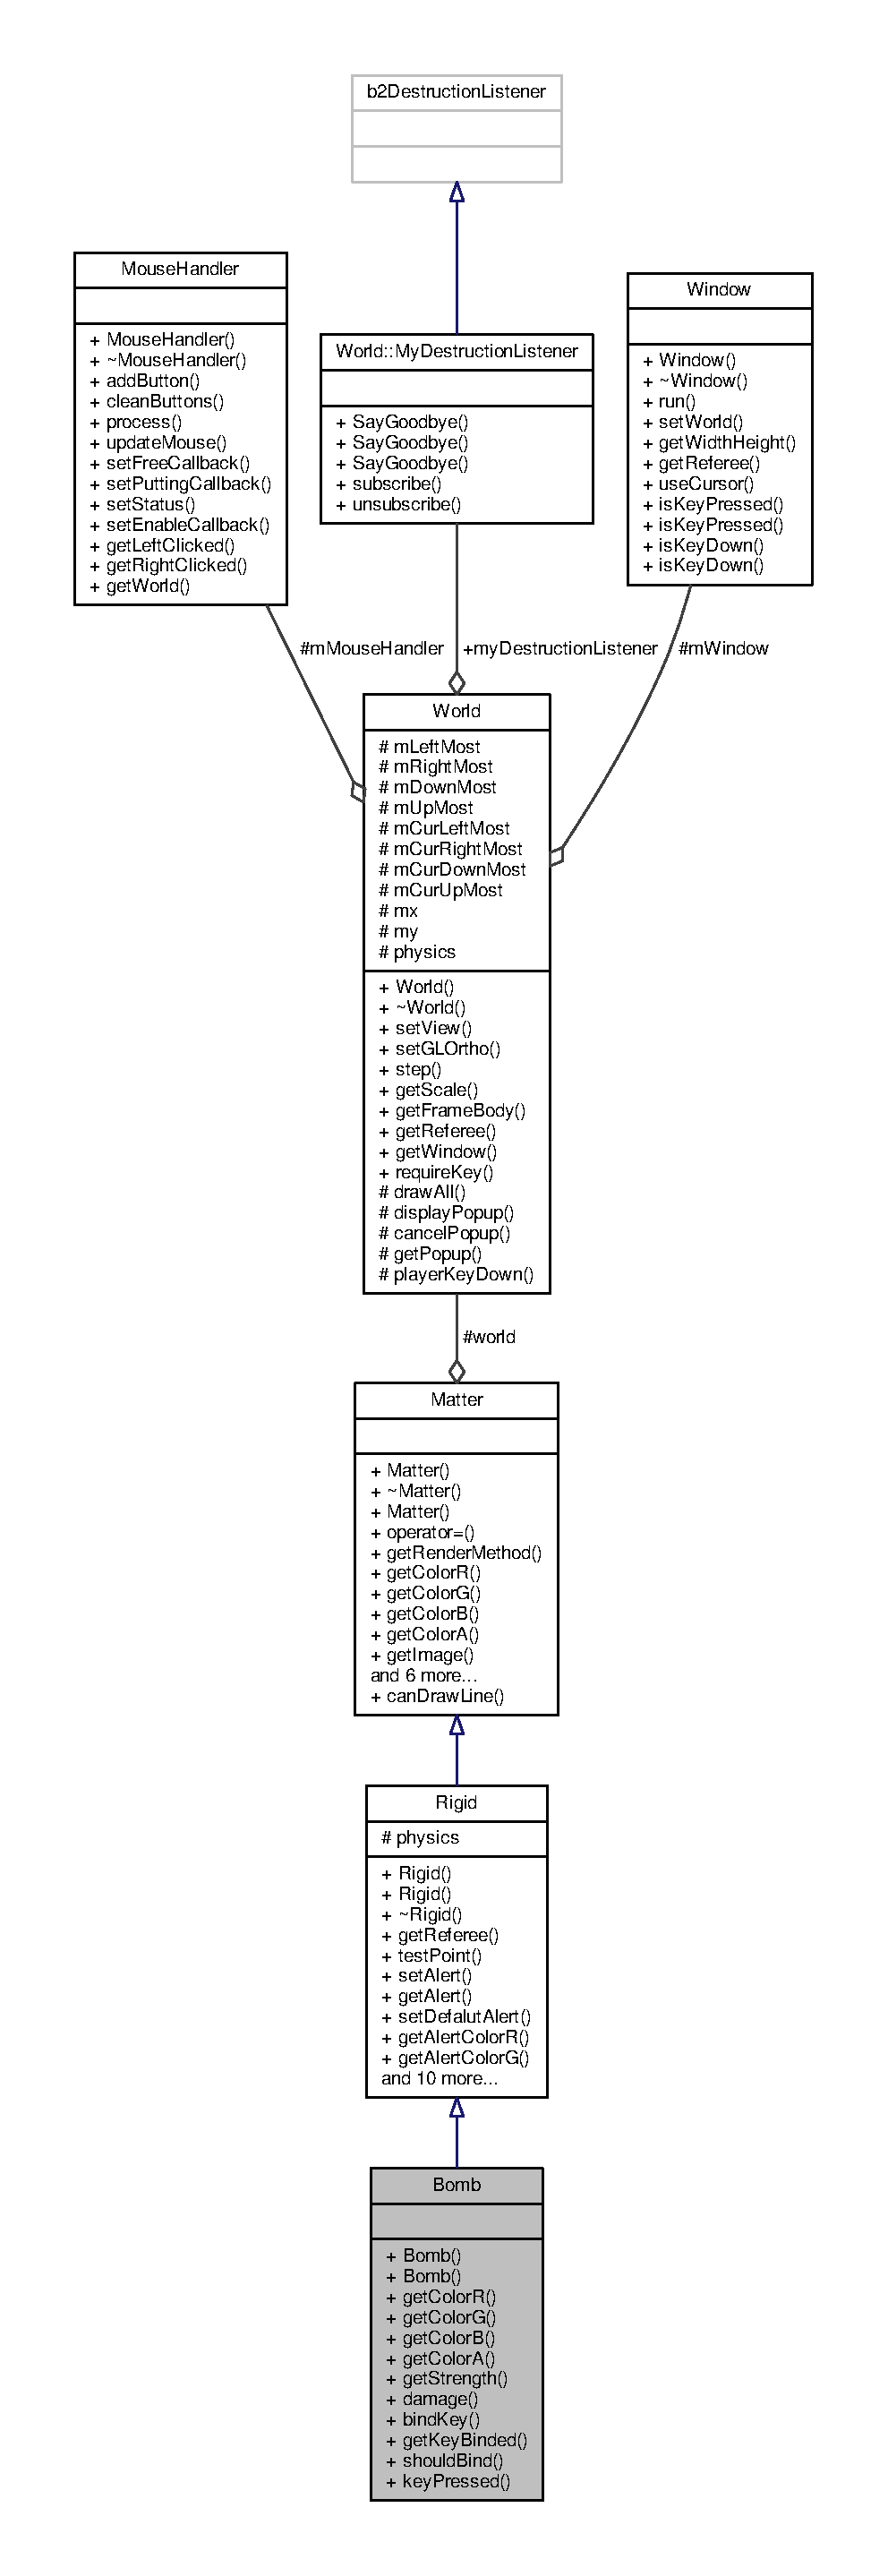
\includegraphics[height=550pt]{classBomb__coll__graph}
\end{center}
\end{figure}
\subsection*{Public Member Functions}
\begin{DoxyCompactItemize}
\item 
\hyperlink{classBomb_a99f489e0cc76550410a9cc59aff6a22e}{Bomb} (\hyperlink{classWorld}{World} $\ast$\+\_\+world, b2\+Body $\ast$\hyperlink{image_8h_ab2d05693952610f937e5acb3c4a8fa1b}{b})
\item 
\hyperlink{classBomb_a0f6e7d6049ed0415cdd2ae811592555e}{Bomb} (\hyperlink{classWorld}{World} $\ast$\+\_\+world, float x, float y, float notused1=0, float notused2=0) noexcept
\item 
virtual float \hyperlink{classBomb_aa95b13c06660f7eaee26dbb75cda41ed}{get\+Color\+R} () const override
\item 
virtual float \hyperlink{classBomb_a393fa1faa9cfdadb0d0202983de6e16b}{get\+Color\+G} () const override
\item 
virtual float \hyperlink{classBomb_a31ede414b7c9c3ef82ea201975d7fd25}{get\+Color\+B} () const override
\item 
virtual float \hyperlink{classBomb_a19e85b4632b547de51bde57844065efa}{get\+Color\+A} () const override
\item 
virtual float \hyperlink{classBomb_a6b09b40f7fb92d9145da7c1c1fe087cb}{get\+Strength} () const override
\begin{DoxyCompactList}\small\item\em rigids are undestroyable by default \end{DoxyCompactList}\item 
void \hyperlink{classBomb_a2bbbb0e9a6972b8276ec19ccac4daa7c}{damage} () override
\begin{DoxyCompactList}\small\item\em create a damage effect and delete the rigid \end{DoxyCompactList}\item 
void \hyperlink{classBomb_a68b2be434320ab67f9000e545b3dcfcd}{bind\+Key} (int \+\_\+key) override
\begin{DoxyCompactList}\small\item\em bind a key on the keyboard to control it 0 = none \end{DoxyCompactList}\item 
int \hyperlink{classBomb_a3e7950bb3de74e07e738a7f94b92a860}{get\+Key\+Binded} () const override
\begin{DoxyCompactList}\small\item\em what has it bind? \end{DoxyCompactList}\item 
bool \hyperlink{classBomb_a3d417c9a938026479149709b76f43b6a}{should\+Bind} () const override
\begin{DoxyCompactList}\small\item\em shoud we bind a key to it? \end{DoxyCompactList}\item 
void \hyperlink{classBomb_a9fe5b989387cc07b82b3da3ccfc3d0db}{key\+Pressed} () override
\begin{DoxyCompactList}\small\item\em what should it do when the key above is pressed \end{DoxyCompactList}\end{DoxyCompactItemize}
\subsection*{Additional Inherited Members}


\subsection{Detailed Description}
r=0.\+5 round bomb 

\subsection{Constructor \& Destructor Documentation}
\hypertarget{classBomb_a99f489e0cc76550410a9cc59aff6a22e}{}\index{Bomb@{Bomb}!Bomb@{Bomb}}
\index{Bomb@{Bomb}!Bomb@{Bomb}}
\subsubsection[{Bomb}]{\setlength{\rightskip}{0pt plus 5cm}Bomb\+::\+Bomb (
\begin{DoxyParamCaption}
\item[{{\bf World} $\ast$}]{\+\_\+world, }
\item[{b2\+Body $\ast$}]{b}
\end{DoxyParamCaption}
)\hspace{0.3cm}{\ttfamily [inline]}}\label{classBomb_a99f489e0cc76550410a9cc59aff6a22e}
\hypertarget{classBomb_a0f6e7d6049ed0415cdd2ae811592555e}{}\index{Bomb@{Bomb}!Bomb@{Bomb}}
\index{Bomb@{Bomb}!Bomb@{Bomb}}
\subsubsection[{Bomb}]{\setlength{\rightskip}{0pt plus 5cm}Bomb\+::\+Bomb (
\begin{DoxyParamCaption}
\item[{{\bf World} $\ast$}]{\+\_\+world, }
\item[{float}]{x, }
\item[{float}]{y, }
\item[{float}]{notused1 = {\ttfamily 0}, }
\item[{float}]{notused2 = {\ttfamily 0}}
\end{DoxyParamCaption}
)\hspace{0.3cm}{\ttfamily [noexcept]}}\label{classBomb_a0f6e7d6049ed0415cdd2ae811592555e}


\subsection{Member Function Documentation}
\hypertarget{classBomb_a68b2be434320ab67f9000e545b3dcfcd}{}\index{Bomb@{Bomb}!bind\+Key@{bind\+Key}}
\index{bind\+Key@{bind\+Key}!Bomb@{Bomb}}
\subsubsection[{bind\+Key}]{\setlength{\rightskip}{0pt plus 5cm}void Bomb\+::bind\+Key (
\begin{DoxyParamCaption}
\item[{int}]{\+\_\+key}
\end{DoxyParamCaption}
)\hspace{0.3cm}{\ttfamily [inline]}, {\ttfamily [override]}, {\ttfamily [virtual]}}\label{classBomb_a68b2be434320ab67f9000e545b3dcfcd}


bind a key on the keyboard to control it 0 = none 



Reimplemented from \hyperlink{classRigid_a5d8922b10420ad452b6d9400d5ecc511}{Rigid}.

\hypertarget{classBomb_a2bbbb0e9a6972b8276ec19ccac4daa7c}{}\index{Bomb@{Bomb}!damage@{damage}}
\index{damage@{damage}!Bomb@{Bomb}}
\subsubsection[{damage}]{\setlength{\rightskip}{0pt plus 5cm}void Bomb\+::damage (
\begin{DoxyParamCaption}
{}
\end{DoxyParamCaption}
)\hspace{0.3cm}{\ttfamily [override]}, {\ttfamily [virtual]}}\label{classBomb_a2bbbb0e9a6972b8276ec19ccac4daa7c}


create a damage effect and delete the rigid 



Reimplemented from \hyperlink{classRigid_a0b64c3d4381acc32987c18d6746f8e35}{Rigid}.

\hypertarget{classBomb_a19e85b4632b547de51bde57844065efa}{}\index{Bomb@{Bomb}!get\+Color\+A@{get\+Color\+A}}
\index{get\+Color\+A@{get\+Color\+A}!Bomb@{Bomb}}
\subsubsection[{get\+Color\+A}]{\setlength{\rightskip}{0pt plus 5cm}virtual float Bomb\+::get\+Color\+A (
\begin{DoxyParamCaption}
{}
\end{DoxyParamCaption}
) const\hspace{0.3cm}{\ttfamily [inline]}, {\ttfamily [override]}, {\ttfamily [virtual]}}\label{classBomb_a19e85b4632b547de51bde57844065efa}


Reimplemented from \hyperlink{classMatter_aa44ee7ba48cb9a582a6f86e1e9e2ef38}{Matter}.

\hypertarget{classBomb_a31ede414b7c9c3ef82ea201975d7fd25}{}\index{Bomb@{Bomb}!get\+Color\+B@{get\+Color\+B}}
\index{get\+Color\+B@{get\+Color\+B}!Bomb@{Bomb}}
\subsubsection[{get\+Color\+B}]{\setlength{\rightskip}{0pt plus 5cm}virtual float Bomb\+::get\+Color\+B (
\begin{DoxyParamCaption}
{}
\end{DoxyParamCaption}
) const\hspace{0.3cm}{\ttfamily [inline]}, {\ttfamily [override]}, {\ttfamily [virtual]}}\label{classBomb_a31ede414b7c9c3ef82ea201975d7fd25}


Reimplemented from \hyperlink{classMatter_af830da17da427c84c7f6deee4a91b3d4}{Matter}.

\hypertarget{classBomb_a393fa1faa9cfdadb0d0202983de6e16b}{}\index{Bomb@{Bomb}!get\+Color\+G@{get\+Color\+G}}
\index{get\+Color\+G@{get\+Color\+G}!Bomb@{Bomb}}
\subsubsection[{get\+Color\+G}]{\setlength{\rightskip}{0pt plus 5cm}virtual float Bomb\+::get\+Color\+G (
\begin{DoxyParamCaption}
{}
\end{DoxyParamCaption}
) const\hspace{0.3cm}{\ttfamily [inline]}, {\ttfamily [override]}, {\ttfamily [virtual]}}\label{classBomb_a393fa1faa9cfdadb0d0202983de6e16b}


Reimplemented from \hyperlink{classMatter_aa3fcdc82f788fbf873ec3ff4808f614a}{Matter}.

\hypertarget{classBomb_aa95b13c06660f7eaee26dbb75cda41ed}{}\index{Bomb@{Bomb}!get\+Color\+R@{get\+Color\+R}}
\index{get\+Color\+R@{get\+Color\+R}!Bomb@{Bomb}}
\subsubsection[{get\+Color\+R}]{\setlength{\rightskip}{0pt plus 5cm}virtual float Bomb\+::get\+Color\+R (
\begin{DoxyParamCaption}
{}
\end{DoxyParamCaption}
) const\hspace{0.3cm}{\ttfamily [inline]}, {\ttfamily [override]}, {\ttfamily [virtual]}}\label{classBomb_aa95b13c06660f7eaee26dbb75cda41ed}


Reimplemented from \hyperlink{classMatter_a926d246584228c3e3b102dbfd42036ec}{Matter}.

\hypertarget{classBomb_a3e7950bb3de74e07e738a7f94b92a860}{}\index{Bomb@{Bomb}!get\+Key\+Binded@{get\+Key\+Binded}}
\index{get\+Key\+Binded@{get\+Key\+Binded}!Bomb@{Bomb}}
\subsubsection[{get\+Key\+Binded}]{\setlength{\rightskip}{0pt plus 5cm}int Bomb\+::get\+Key\+Binded (
\begin{DoxyParamCaption}
{}
\end{DoxyParamCaption}
) const\hspace{0.3cm}{\ttfamily [inline]}, {\ttfamily [override]}, {\ttfamily [virtual]}}\label{classBomb_a3e7950bb3de74e07e738a7f94b92a860}


what has it bind? 



Reimplemented from \hyperlink{classRigid_a4e5382b25c00ff97745b04120e51cb56}{Rigid}.

\hypertarget{classBomb_a6b09b40f7fb92d9145da7c1c1fe087cb}{}\index{Bomb@{Bomb}!get\+Strength@{get\+Strength}}
\index{get\+Strength@{get\+Strength}!Bomb@{Bomb}}
\subsubsection[{get\+Strength}]{\setlength{\rightskip}{0pt plus 5cm}virtual float Bomb\+::get\+Strength (
\begin{DoxyParamCaption}
{}
\end{DoxyParamCaption}
) const\hspace{0.3cm}{\ttfamily [inline]}, {\ttfamily [override]}, {\ttfamily [virtual]}}\label{classBomb_a6b09b40f7fb92d9145da7c1c1fe087cb}


rigids are undestroyable by default 



Reimplemented from \hyperlink{classRigid_aac83bf941605a8cbccf06a5d4b200fee}{Rigid}.

\hypertarget{classBomb_a9fe5b989387cc07b82b3da3ccfc3d0db}{}\index{Bomb@{Bomb}!key\+Pressed@{key\+Pressed}}
\index{key\+Pressed@{key\+Pressed}!Bomb@{Bomb}}
\subsubsection[{key\+Pressed}]{\setlength{\rightskip}{0pt plus 5cm}void Bomb\+::key\+Pressed (
\begin{DoxyParamCaption}
{}
\end{DoxyParamCaption}
)\hspace{0.3cm}{\ttfamily [inline]}, {\ttfamily [override]}, {\ttfamily [virtual]}}\label{classBomb_a9fe5b989387cc07b82b3da3ccfc3d0db}


what should it do when the key above is pressed 



Reimplemented from \hyperlink{classRigid_a769957138e3ca40a4a6b1da4cf52eea8}{Rigid}.

\hypertarget{classBomb_a3d417c9a938026479149709b76f43b6a}{}\index{Bomb@{Bomb}!should\+Bind@{should\+Bind}}
\index{should\+Bind@{should\+Bind}!Bomb@{Bomb}}
\subsubsection[{should\+Bind}]{\setlength{\rightskip}{0pt plus 5cm}bool Bomb\+::should\+Bind (
\begin{DoxyParamCaption}
{}
\end{DoxyParamCaption}
) const\hspace{0.3cm}{\ttfamily [inline]}, {\ttfamily [override]}, {\ttfamily [virtual]}}\label{classBomb_a3d417c9a938026479149709b76f43b6a}


shoud we bind a key to it? 



Reimplemented from \hyperlink{classRigid_a213d4ddd819ea799b7a29961b0d66f39}{Rigid}.



The documentation for this class was generated from the following files\+:\begin{DoxyCompactItemize}
\item 
\hyperlink{matter_8h}{matter.\+h}\item 
\hyperlink{matter_8cpp}{matter.\+cpp}\end{DoxyCompactItemize}

\hypertarget{classButton}{}\section{Button$<$ image\+Name $>$ Class Template Reference}
\label{classButton}\index{Button$<$ image\+Name $>$@{Button$<$ image\+Name $>$}}


{\ttfamily \#include $<$matter.\+h$>$}



Inheritance diagram for Button$<$ image\+Name $>$\+:
\nopagebreak
\begin{figure}[H]
\begin{center}
\leavevmode
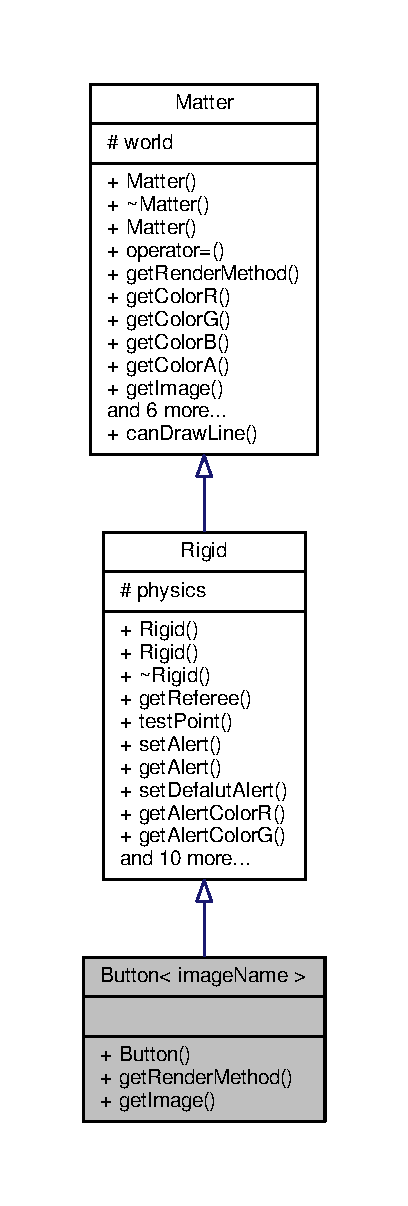
\includegraphics[height=550pt]{classButton__inherit__graph}
\end{center}
\end{figure}


Collaboration diagram for Button$<$ image\+Name $>$\+:
\nopagebreak
\begin{figure}[H]
\begin{center}
\leavevmode
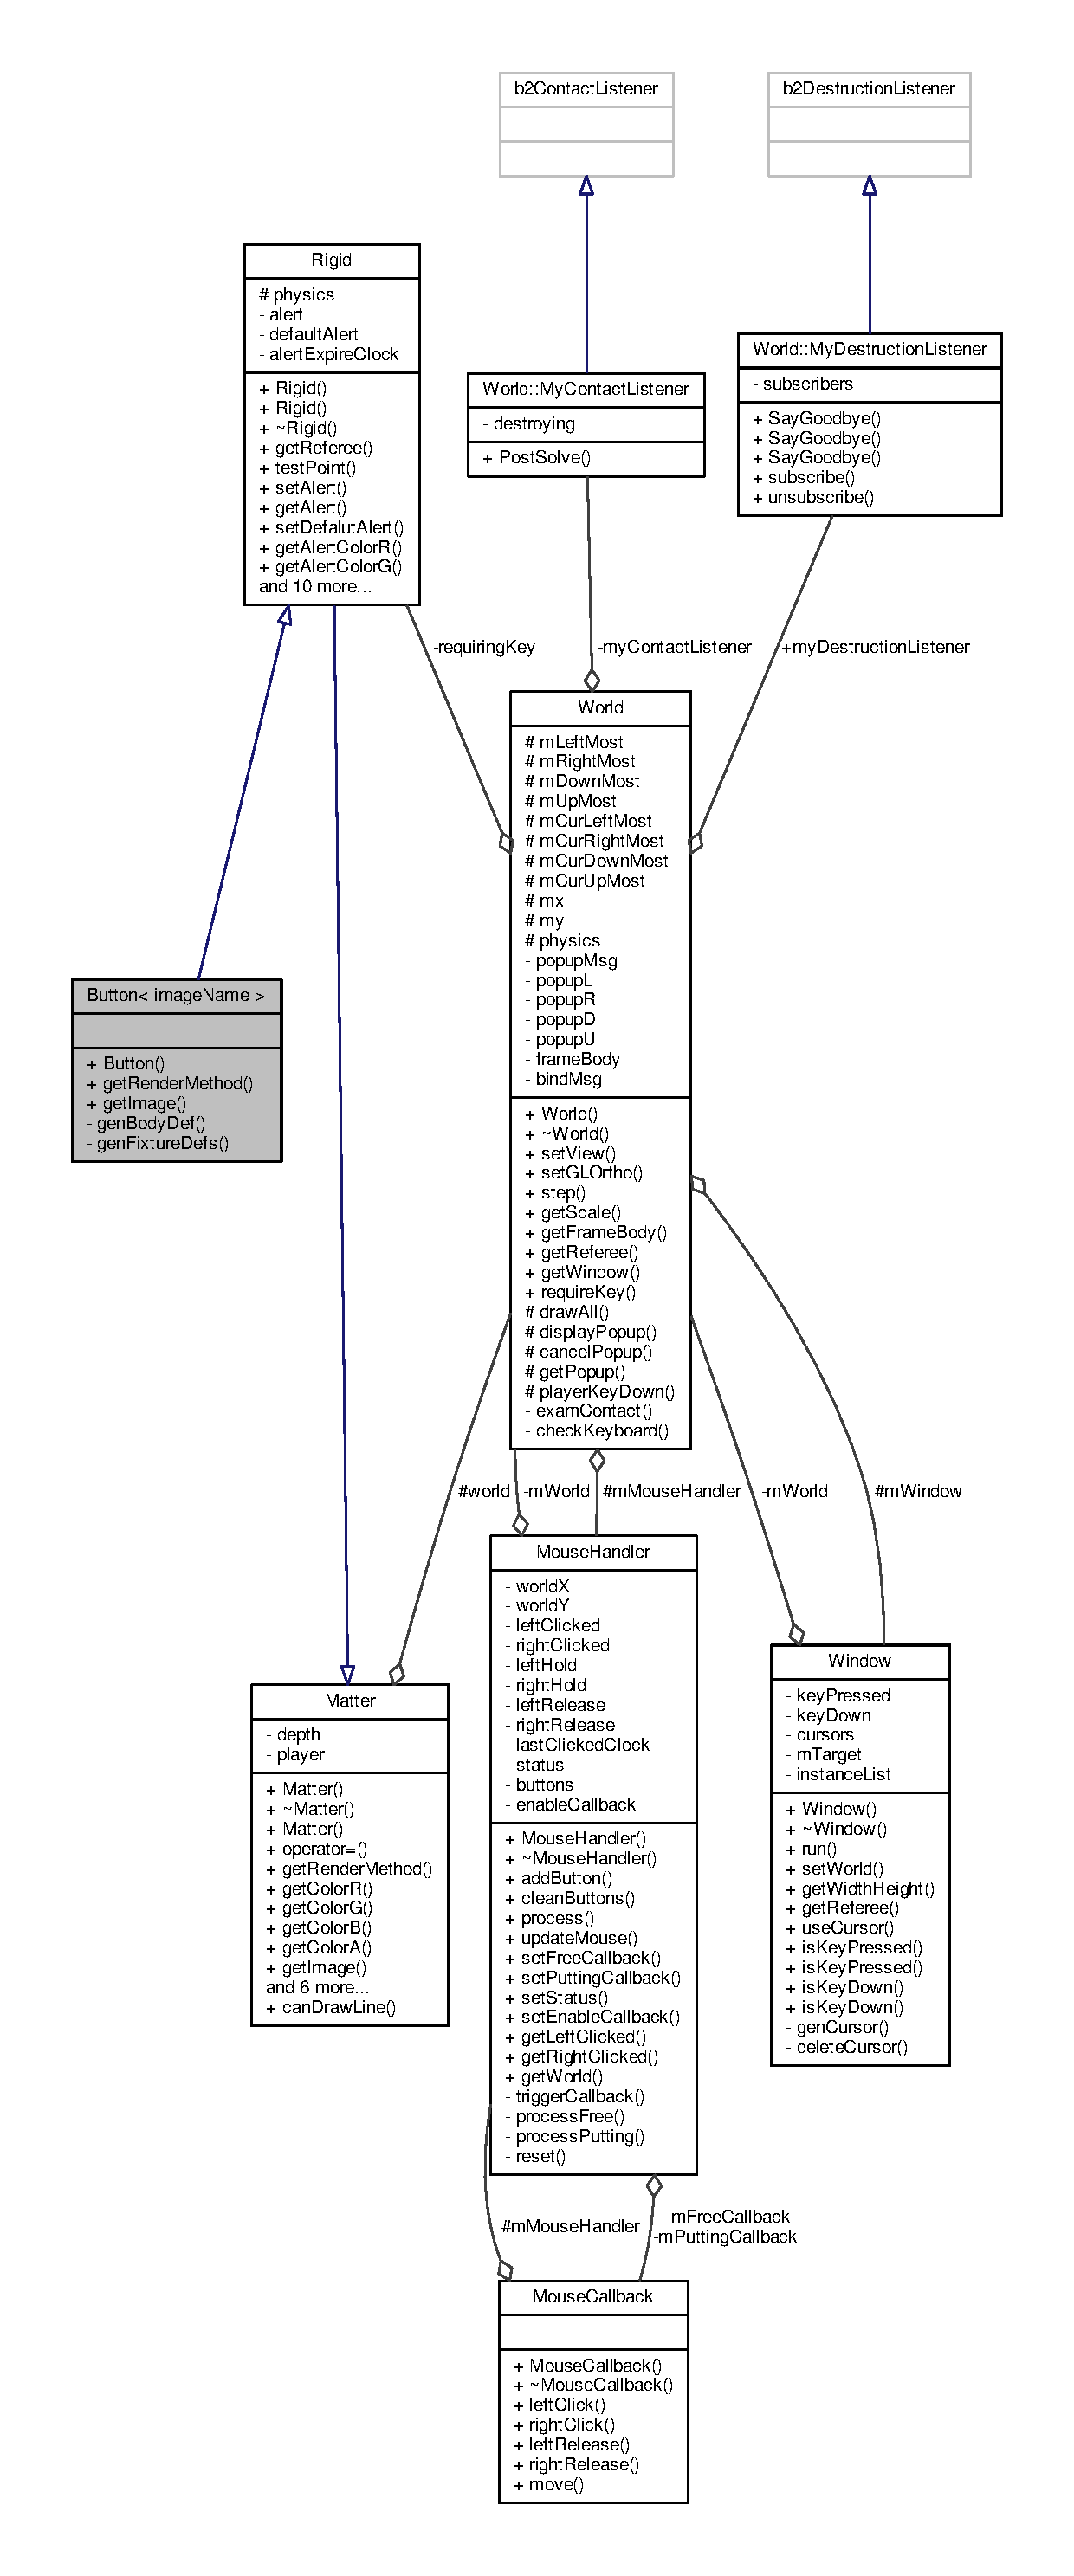
\includegraphics[height=550pt]{classButton__coll__graph}
\end{center}
\end{figure}
\subsection*{Public Member Functions}
\begin{DoxyCompactItemize}
\item 
\hyperlink{classButton_a36705b8de68995c157c107af83e94644}{Button} (\hyperlink{classWorld}{World} $\ast$\+\_\+world, float l, float \hyperlink{image_8h_a62969232668331297e2dca1ae2ddd10d}{r}, float d, float u) noexcept
\item 
virtual \hyperlink{classMatter_ade1ce1bf81f25377f689d103cd431907}{Render\+Method} \hyperlink{classButton_a50233f0c531652154ecc0f8f7dc26571}{get\+Render\+Method} () const override
\item 
virtual \hyperlink{image_8h_af9361b398b5cfcafbe93f82e8eaeb080}{Image\+Name} \hyperlink{classButton_a75331f4a815ee394a223812681460e09}{get\+Image} () const override
\end{DoxyCompactItemize}
\subsection*{Static Private Member Functions}
\begin{DoxyCompactItemize}
\item 
static b2\+Body\+Def \hyperlink{classButton_af51953ff1e1270670f813aa851d71e0a}{gen\+Body\+Def} (float l, float \hyperlink{image_8h_a62969232668331297e2dca1ae2ddd10d}{r}, float d, float u)
\item 
static std\+::vector$<$ b2\+Fixture\+Def $>$ \hyperlink{classButton_a61ef71e88eb48e02909c9e0b3e5f9f28}{gen\+Fixture\+Defs} (float l, float \hyperlink{image_8h_a62969232668331297e2dca1ae2ddd10d}{r}, float d, float u)
\end{DoxyCompactItemize}
\subsection*{Additional Inherited Members}


\subsection{Constructor \& Destructor Documentation}
\hypertarget{classButton_a36705b8de68995c157c107af83e94644}{}\index{Button@{Button}!Button@{Button}}
\index{Button@{Button}!Button@{Button}}
\subsubsection[{Button}]{\setlength{\rightskip}{0pt plus 5cm}template$<$Image\+Name image\+Name$>$ {\bf Button}$<$ image\+Name $>$\+::{\bf Button} (
\begin{DoxyParamCaption}
\item[{{\bf World} $\ast$}]{\+\_\+world, }
\item[{float}]{l, }
\item[{float}]{r, }
\item[{float}]{d, }
\item[{float}]{u}
\end{DoxyParamCaption}
)\hspace{0.3cm}{\ttfamily [inline]}, {\ttfamily [noexcept]}}\label{classButton_a36705b8de68995c157c107af83e94644}


\subsection{Member Function Documentation}
\hypertarget{classButton_af51953ff1e1270670f813aa851d71e0a}{}\index{Button@{Button}!gen\+Body\+Def@{gen\+Body\+Def}}
\index{gen\+Body\+Def@{gen\+Body\+Def}!Button@{Button}}
\subsubsection[{gen\+Body\+Def}]{\setlength{\rightskip}{0pt plus 5cm}template$<$Image\+Name image\+Name$>$ b2\+Body\+Def {\bf Button}$<$ image\+Name $>$\+::gen\+Body\+Def (
\begin{DoxyParamCaption}
\item[{float}]{l, }
\item[{float}]{r, }
\item[{float}]{d, }
\item[{float}]{u}
\end{DoxyParamCaption}
)\hspace{0.3cm}{\ttfamily [static]}, {\ttfamily [private]}}\label{classButton_af51953ff1e1270670f813aa851d71e0a}
\hypertarget{classButton_a61ef71e88eb48e02909c9e0b3e5f9f28}{}\index{Button@{Button}!gen\+Fixture\+Defs@{gen\+Fixture\+Defs}}
\index{gen\+Fixture\+Defs@{gen\+Fixture\+Defs}!Button@{Button}}
\subsubsection[{gen\+Fixture\+Defs}]{\setlength{\rightskip}{0pt plus 5cm}template$<$Image\+Name image\+Name$>$ std\+::vector$<$ b2\+Fixture\+Def $>$ {\bf Button}$<$ image\+Name $>$\+::gen\+Fixture\+Defs (
\begin{DoxyParamCaption}
\item[{float}]{l, }
\item[{float}]{r, }
\item[{float}]{d, }
\item[{float}]{u}
\end{DoxyParamCaption}
)\hspace{0.3cm}{\ttfamily [static]}, {\ttfamily [private]}}\label{classButton_a61ef71e88eb48e02909c9e0b3e5f9f28}
\hypertarget{classButton_a75331f4a815ee394a223812681460e09}{}\index{Button@{Button}!get\+Image@{get\+Image}}
\index{get\+Image@{get\+Image}!Button@{Button}}
\subsubsection[{get\+Image}]{\setlength{\rightskip}{0pt plus 5cm}template$<$Image\+Name image\+Name$>$ virtual {\bf Image\+Name} {\bf Button}$<$ image\+Name $>$\+::get\+Image (
\begin{DoxyParamCaption}
{}
\end{DoxyParamCaption}
) const\hspace{0.3cm}{\ttfamily [inline]}, {\ttfamily [override]}, {\ttfamily [virtual]}}\label{classButton_a75331f4a815ee394a223812681460e09}


Reimplemented from \hyperlink{classMatter_ad6202a62e4ae27dde457c56520f1865e}{Matter}.

\hypertarget{classButton_a50233f0c531652154ecc0f8f7dc26571}{}\index{Button@{Button}!get\+Render\+Method@{get\+Render\+Method}}
\index{get\+Render\+Method@{get\+Render\+Method}!Button@{Button}}
\subsubsection[{get\+Render\+Method}]{\setlength{\rightskip}{0pt plus 5cm}template$<$Image\+Name image\+Name$>$ virtual {\bf Render\+Method} {\bf Button}$<$ image\+Name $>$\+::get\+Render\+Method (
\begin{DoxyParamCaption}
{}
\end{DoxyParamCaption}
) const\hspace{0.3cm}{\ttfamily [inline]}, {\ttfamily [override]}, {\ttfamily [virtual]}}\label{classButton_a50233f0c531652154ecc0f8f7dc26571}


Reimplemented from \hyperlink{classMatter_a3d6823a375fe0a537837b905b44af5bd}{Matter}.



The documentation for this class was generated from the following file\+:\begin{DoxyCompactItemize}
\item 
\hyperlink{matter_8h}{matter.\+h}\end{DoxyCompactItemize}

\hypertarget{classCancelCallback}{}\section{Cancel\+Callback Class Reference}
\label{classCancelCallback}\index{Cancel\+Callback@{Cancel\+Callback}}


Inheritance diagram for Cancel\+Callback\+:
\nopagebreak
\begin{figure}[H]
\begin{center}
\leavevmode
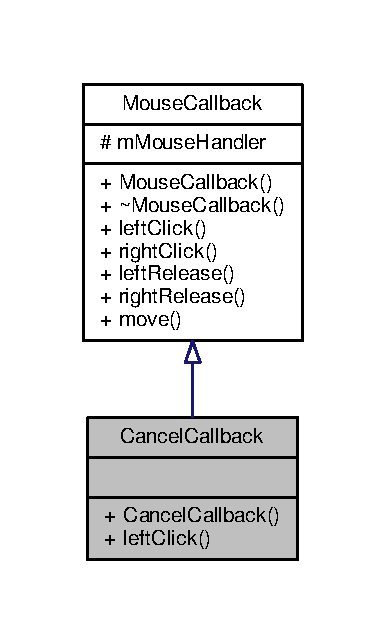
\includegraphics[width=185pt]{classCancelCallback__inherit__graph}
\end{center}
\end{figure}


Collaboration diagram for Cancel\+Callback\+:
\nopagebreak
\begin{figure}[H]
\begin{center}
\leavevmode
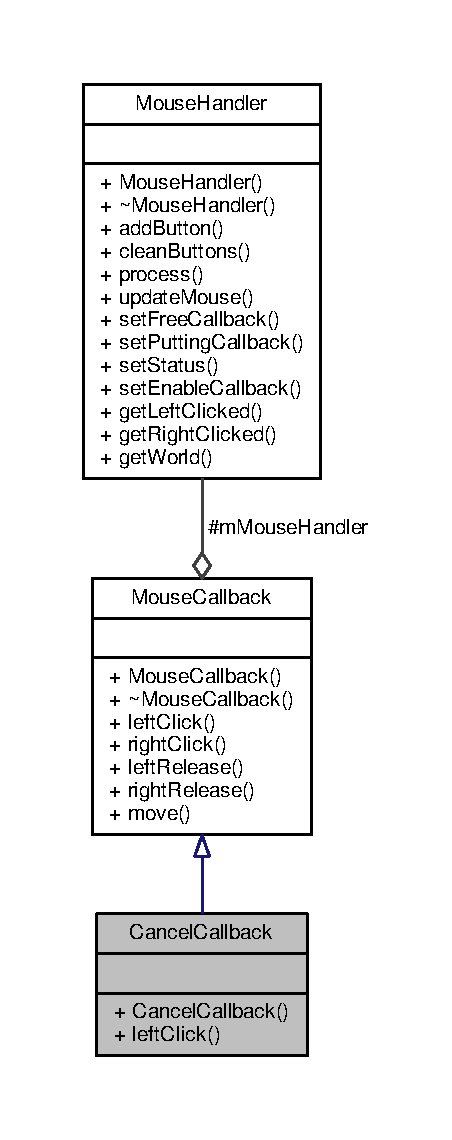
\includegraphics[height=550pt]{classCancelCallback__coll__graph}
\end{center}
\end{figure}
\subsection*{Public Member Functions}
\begin{DoxyCompactItemize}
\item 
\hyperlink{classCancelCallback_a1b0750b3aadf2b1781c3744f5e2da940}{Cancel\+Callback} (\hyperlink{classMouseHandler}{Mouse\+Handler} $\ast$\+\_\+handler)
\item 
void \hyperlink{classCancelCallback_a2cbc9b79d82ab408d767938351b1eb54}{left\+Click} (float, float)
\end{DoxyCompactItemize}
\subsection*{Additional Inherited Members}


\subsection{Constructor \& Destructor Documentation}
\hypertarget{classCancelCallback_a1b0750b3aadf2b1781c3744f5e2da940}{}\index{Cancel\+Callback@{Cancel\+Callback}!Cancel\+Callback@{Cancel\+Callback}}
\index{Cancel\+Callback@{Cancel\+Callback}!Cancel\+Callback@{Cancel\+Callback}}
\subsubsection[{Cancel\+Callback}]{\setlength{\rightskip}{0pt plus 5cm}Cancel\+Callback\+::\+Cancel\+Callback (
\begin{DoxyParamCaption}
\item[{{\bf Mouse\+Handler} $\ast$}]{\+\_\+handler}
\end{DoxyParamCaption}
)\hspace{0.3cm}{\ttfamily [inline]}}\label{classCancelCallback_a1b0750b3aadf2b1781c3744f5e2da940}


\subsection{Member Function Documentation}
\hypertarget{classCancelCallback_a2cbc9b79d82ab408d767938351b1eb54}{}\index{Cancel\+Callback@{Cancel\+Callback}!left\+Click@{left\+Click}}
\index{left\+Click@{left\+Click}!Cancel\+Callback@{Cancel\+Callback}}
\subsubsection[{left\+Click}]{\setlength{\rightskip}{0pt plus 5cm}void Cancel\+Callback\+::left\+Click (
\begin{DoxyParamCaption}
\item[{float}]{, }
\item[{float}]{}
\end{DoxyParamCaption}
)\hspace{0.3cm}{\ttfamily [inline]}, {\ttfamily [virtual]}}\label{classCancelCallback_a2cbc9b79d82ab408d767938351b1eb54}


Reimplemented from \hyperlink{classMouseCallback_a5ae88358471f1b48e3f6a730aaf0ba13}{Mouse\+Callback}.



The documentation for this class was generated from the following file\+:\begin{DoxyCompactItemize}
\item 
\hyperlink{world_8cpp}{world.\+cpp}\end{DoxyCompactItemize}

\hypertarget{classDeleteButtonCallback}{}\section{Delete\+Button\+Callback Class Reference}
\label{classDeleteButtonCallback}\index{Delete\+Button\+Callback@{Delete\+Button\+Callback}}


{\ttfamily \#include $<$mousecallback.\+h$>$}



Inheritance diagram for Delete\+Button\+Callback\+:
\nopagebreak
\begin{figure}[H]
\begin{center}
\leavevmode
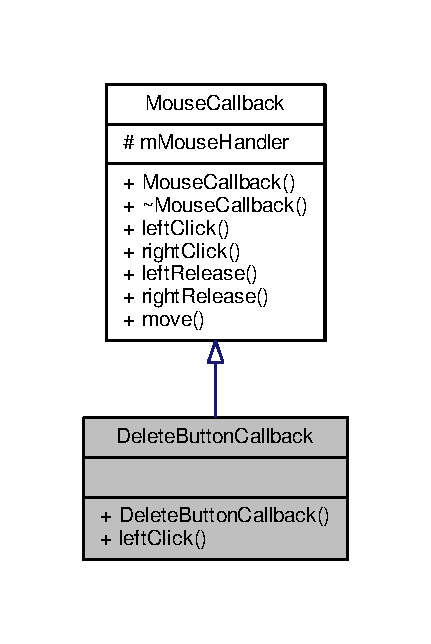
\includegraphics[width=207pt]{classDeleteButtonCallback__inherit__graph}
\end{center}
\end{figure}


Collaboration diagram for Delete\+Button\+Callback\+:
\nopagebreak
\begin{figure}[H]
\begin{center}
\leavevmode
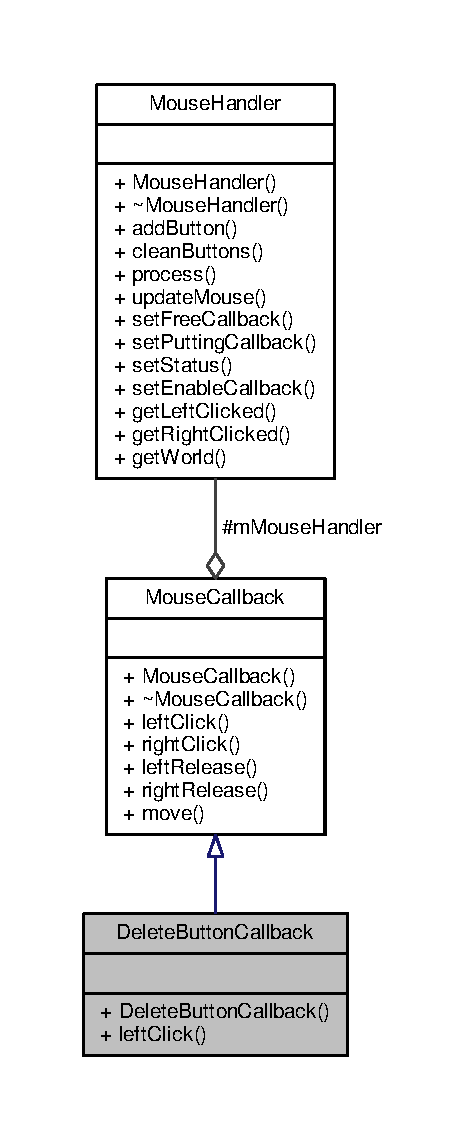
\includegraphics[height=550pt]{classDeleteButtonCallback__coll__graph}
\end{center}
\end{figure}
\subsection*{Public Member Functions}
\begin{DoxyCompactItemize}
\item 
\hyperlink{classDeleteButtonCallback_a54d43b4ae8398816061ac1c170039356}{Delete\+Button\+Callback} (\hyperlink{classMouseHandler}{Mouse\+Handler} $\ast$\+\_\+handler)
\item 
void \hyperlink{classDeleteButtonCallback_ac4332c88d4198bb182c24ce4fb1f85ab}{left\+Click} (float, float) override
\end{DoxyCompactItemize}
\subsection*{Additional Inherited Members}


\subsection{Constructor \& Destructor Documentation}
\hypertarget{classDeleteButtonCallback_a54d43b4ae8398816061ac1c170039356}{}\index{Delete\+Button\+Callback@{Delete\+Button\+Callback}!Delete\+Button\+Callback@{Delete\+Button\+Callback}}
\index{Delete\+Button\+Callback@{Delete\+Button\+Callback}!Delete\+Button\+Callback@{Delete\+Button\+Callback}}
\subsubsection[{Delete\+Button\+Callback}]{\setlength{\rightskip}{0pt plus 5cm}Delete\+Button\+Callback\+::\+Delete\+Button\+Callback (
\begin{DoxyParamCaption}
\item[{{\bf Mouse\+Handler} $\ast$}]{\+\_\+handler}
\end{DoxyParamCaption}
)\hspace{0.3cm}{\ttfamily [inline]}}\label{classDeleteButtonCallback_a54d43b4ae8398816061ac1c170039356}


\subsection{Member Function Documentation}
\hypertarget{classDeleteButtonCallback_ac4332c88d4198bb182c24ce4fb1f85ab}{}\index{Delete\+Button\+Callback@{Delete\+Button\+Callback}!left\+Click@{left\+Click}}
\index{left\+Click@{left\+Click}!Delete\+Button\+Callback@{Delete\+Button\+Callback}}
\subsubsection[{left\+Click}]{\setlength{\rightskip}{0pt plus 5cm}void Delete\+Button\+Callback\+::left\+Click (
\begin{DoxyParamCaption}
\item[{float}]{, }
\item[{float}]{}
\end{DoxyParamCaption}
)\hspace{0.3cm}{\ttfamily [inline]}, {\ttfamily [override]}, {\ttfamily [virtual]}}\label{classDeleteButtonCallback_ac4332c88d4198bb182c24ce4fb1f85ab}


Reimplemented from \hyperlink{classMouseCallback_a5ae88358471f1b48e3f6a730aaf0ba13}{Mouse\+Callback}.



The documentation for this class was generated from the following file\+:\begin{DoxyCompactItemize}
\item 
\hyperlink{mousecallback_8h}{mousecallback.\+h}\end{DoxyCompactItemize}

\hypertarget{classDeletingCallback}{}\section{Deleting\+Callback Class Reference}
\label{classDeletingCallback}\index{Deleting\+Callback@{Deleting\+Callback}}


{\ttfamily \#include $<$mousecallback.\+h$>$}



Inheritance diagram for Deleting\+Callback\+:\nopagebreak
\begin{figure}[H]
\begin{center}
\leavevmode
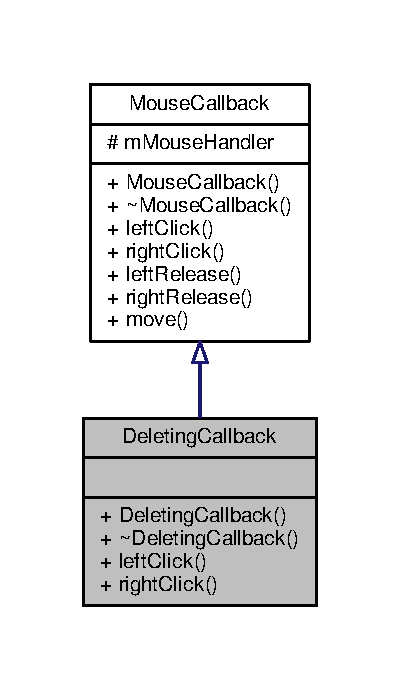
\includegraphics[width=192pt]{classDeletingCallback__inherit__graph}
\end{center}
\end{figure}


Collaboration diagram for Deleting\+Callback\+:
\nopagebreak
\begin{figure}[H]
\begin{center}
\leavevmode
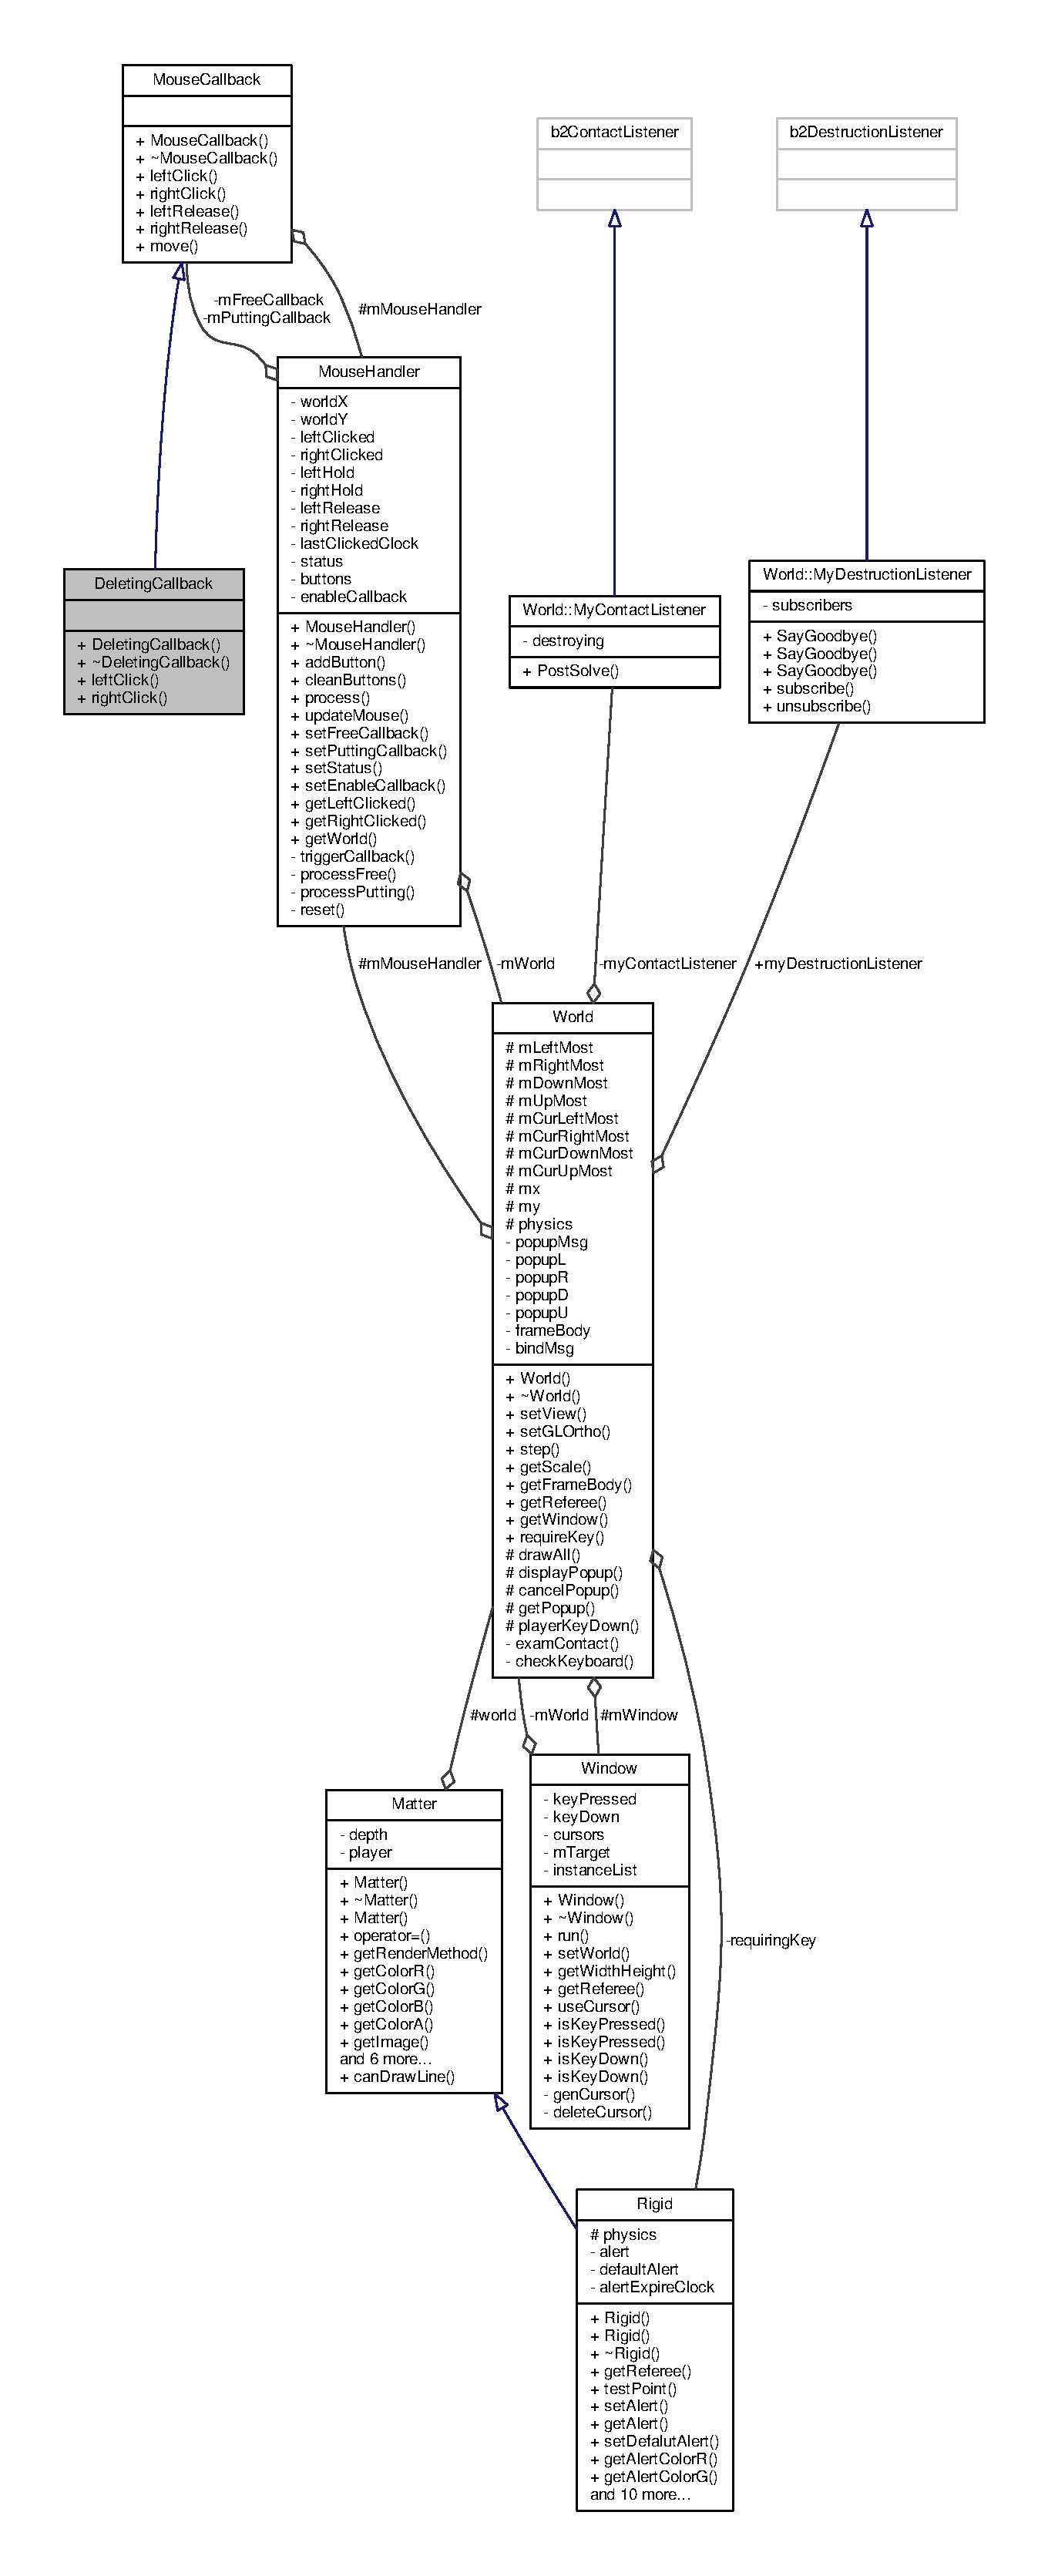
\includegraphics[height=550pt]{classDeletingCallback__coll__graph}
\end{center}
\end{figure}
\subsection*{Public Member Functions}
\begin{DoxyCompactItemize}
\item 
\hyperlink{classDeletingCallback_a839acb7ac22a4f9fccc80e62407ef28e}{Deleting\+Callback} (\hyperlink{classMouseHandler}{Mouse\+Handler} $\ast$\+\_\+handler)
\item 
\hyperlink{classDeletingCallback_a27669af3ef00eedb57180d71077a6447}{$\sim$\+Deleting\+Callback} ()
\item 
void \hyperlink{classDeletingCallback_a99382467c294e9a6410592216ceccb19}{left\+Click} (float x, float y) override
\item 
void \hyperlink{classDeletingCallback_a2c33b247519be8e2e49b938f467d6eec}{right\+Click} (float x, float y) override
\end{DoxyCompactItemize}
\subsection*{Additional Inherited Members}


\subsection{Constructor \& Destructor Documentation}
\hypertarget{classDeletingCallback_a839acb7ac22a4f9fccc80e62407ef28e}{}\index{Deleting\+Callback@{Deleting\+Callback}!Deleting\+Callback@{Deleting\+Callback}}
\index{Deleting\+Callback@{Deleting\+Callback}!Deleting\+Callback@{Deleting\+Callback}}
\subsubsection[{Deleting\+Callback}]{\setlength{\rightskip}{0pt plus 5cm}Deleting\+Callback\+::\+Deleting\+Callback (
\begin{DoxyParamCaption}
\item[{{\bf Mouse\+Handler} $\ast$}]{\+\_\+handler}
\end{DoxyParamCaption}
)\hspace{0.3cm}{\ttfamily [inline]}}\label{classDeletingCallback_a839acb7ac22a4f9fccc80e62407ef28e}
\hypertarget{classDeletingCallback_a27669af3ef00eedb57180d71077a6447}{}\index{Deleting\+Callback@{Deleting\+Callback}!````~Deleting\+Callback@{$\sim$\+Deleting\+Callback}}
\index{````~Deleting\+Callback@{$\sim$\+Deleting\+Callback}!Deleting\+Callback@{Deleting\+Callback}}
\subsubsection[{$\sim$\+Deleting\+Callback}]{\setlength{\rightskip}{0pt plus 5cm}Deleting\+Callback\+::$\sim$\+Deleting\+Callback (
\begin{DoxyParamCaption}
{}
\end{DoxyParamCaption}
)\hspace{0.3cm}{\ttfamily [inline]}}\label{classDeletingCallback_a27669af3ef00eedb57180d71077a6447}


\subsection{Member Function Documentation}
\hypertarget{classDeletingCallback_a99382467c294e9a6410592216ceccb19}{}\index{Deleting\+Callback@{Deleting\+Callback}!left\+Click@{left\+Click}}
\index{left\+Click@{left\+Click}!Deleting\+Callback@{Deleting\+Callback}}
\subsubsection[{left\+Click}]{\setlength{\rightskip}{0pt plus 5cm}void Deleting\+Callback\+::left\+Click (
\begin{DoxyParamCaption}
\item[{float}]{x, }
\item[{float}]{y}
\end{DoxyParamCaption}
)\hspace{0.3cm}{\ttfamily [inline]}, {\ttfamily [override]}, {\ttfamily [virtual]}}\label{classDeletingCallback_a99382467c294e9a6410592216ceccb19}


Reimplemented from \hyperlink{classMouseCallback_a5ae88358471f1b48e3f6a730aaf0ba13}{Mouse\+Callback}.

\hypertarget{classDeletingCallback_a2c33b247519be8e2e49b938f467d6eec}{}\index{Deleting\+Callback@{Deleting\+Callback}!right\+Click@{right\+Click}}
\index{right\+Click@{right\+Click}!Deleting\+Callback@{Deleting\+Callback}}
\subsubsection[{right\+Click}]{\setlength{\rightskip}{0pt plus 5cm}void Deleting\+Callback\+::right\+Click (
\begin{DoxyParamCaption}
\item[{float}]{x, }
\item[{float}]{y}
\end{DoxyParamCaption}
)\hspace{0.3cm}{\ttfamily [inline]}, {\ttfamily [override]}, {\ttfamily [virtual]}}\label{classDeletingCallback_a2c33b247519be8e2e49b938f467d6eec}


Reimplemented from \hyperlink{classMouseCallback_aa4a0c30b50b48972d0a48b9aff6344c5}{Mouse\+Callback}.



The documentation for this class was generated from the following file\+:\begin{DoxyCompactItemize}
\item 
\hyperlink{mousecallback_8h}{mousecallback.\+h}\end{DoxyCompactItemize}

\hypertarget{classDraggingCallback}{}\section{Dragging\+Callback Class Reference}
\label{classDraggingCallback}\index{Dragging\+Callback@{Dragging\+Callback}}


{\ttfamily \#include $<$mousecallback.\+h$>$}



Inheritance diagram for Dragging\+Callback\+:\nopagebreak
\begin{figure}[H]
\begin{center}
\leavevmode
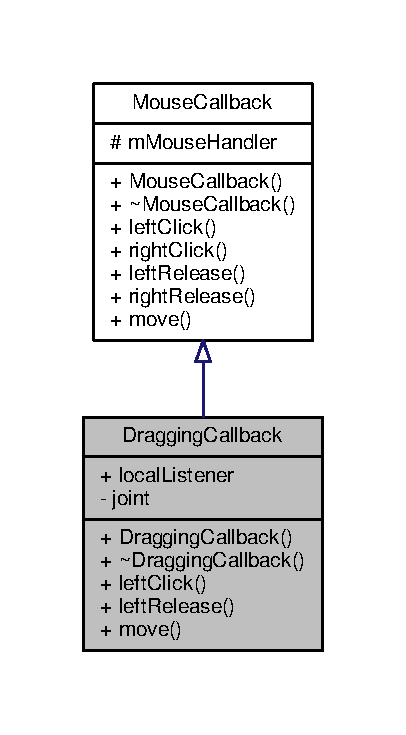
\includegraphics[width=195pt]{classDraggingCallback__inherit__graph}
\end{center}
\end{figure}


Collaboration diagram for Dragging\+Callback\+:\nopagebreak
\begin{figure}[H]
\begin{center}
\leavevmode
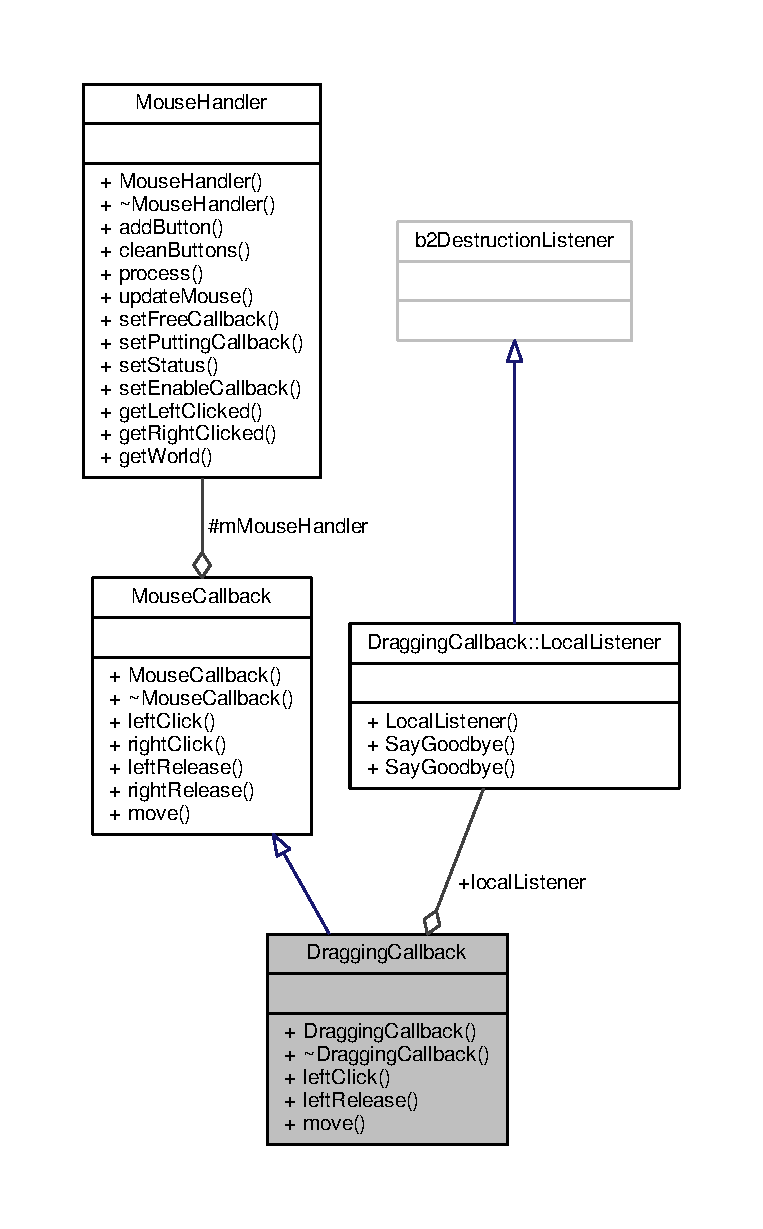
\includegraphics[height=550pt]{classDraggingCallback__coll__graph}
\end{center}
\end{figure}
\subsection*{Classes}
\begin{DoxyCompactItemize}
\item 
class \hyperlink{classDraggingCallback_1_1LocalListener}{Local\+Listener}
\end{DoxyCompactItemize}
\subsection*{Public Member Functions}
\begin{DoxyCompactItemize}
\item 
\hyperlink{classDraggingCallback_a9ea246a89d494379fd518cf544694674}{Dragging\+Callback} (\hyperlink{classMouseHandler}{Mouse\+Handler} $\ast$\+\_\+handler)
\item 
\hyperlink{classDraggingCallback_a47830632e5c0894a2883af00817d58dc}{$\sim$\+Dragging\+Callback} ()
\item 
void \hyperlink{classDraggingCallback_a20b673ac127fd52f7bf8453467930cf5}{left\+Click} (float x, float y) override
\item 
void \hyperlink{classDraggingCallback_a33ea59d939d8e3fa366e595628e8ac4f}{left\+Release} (float, float) override
\item 
void \hyperlink{classDraggingCallback_a8d1541c9219f67864ab64279b53d3ad4}{move} (float x, float y) override
\end{DoxyCompactItemize}
\subsection*{Public Attributes}
\begin{DoxyCompactItemize}
\item 
\hyperlink{classDraggingCallback_1_1LocalListener}{Dragging\+Callback\+::\+Local\+Listener} \hyperlink{classDraggingCallback_a65aaf71fa563b3976df8407611cbfd39}{local\+Listener}
\end{DoxyCompactItemize}
\subsection*{Additional Inherited Members}


\subsection{Constructor \& Destructor Documentation}
\hypertarget{classDraggingCallback_a9ea246a89d494379fd518cf544694674}{}\index{Dragging\+Callback@{Dragging\+Callback}!Dragging\+Callback@{Dragging\+Callback}}
\index{Dragging\+Callback@{Dragging\+Callback}!Dragging\+Callback@{Dragging\+Callback}}
\subsubsection[{Dragging\+Callback}]{\setlength{\rightskip}{0pt plus 5cm}Dragging\+Callback\+::\+Dragging\+Callback (
\begin{DoxyParamCaption}
\item[{{\bf Mouse\+Handler} $\ast$}]{\+\_\+handler}
\end{DoxyParamCaption}
)\hspace{0.3cm}{\ttfamily [inline]}}\label{classDraggingCallback_a9ea246a89d494379fd518cf544694674}
\hypertarget{classDraggingCallback_a47830632e5c0894a2883af00817d58dc}{}\index{Dragging\+Callback@{Dragging\+Callback}!````~Dragging\+Callback@{$\sim$\+Dragging\+Callback}}
\index{````~Dragging\+Callback@{$\sim$\+Dragging\+Callback}!Dragging\+Callback@{Dragging\+Callback}}
\subsubsection[{$\sim$\+Dragging\+Callback}]{\setlength{\rightskip}{0pt plus 5cm}Dragging\+Callback\+::$\sim$\+Dragging\+Callback (
\begin{DoxyParamCaption}
{}
\end{DoxyParamCaption}
)\hspace{0.3cm}{\ttfamily [inline]}}\label{classDraggingCallback_a47830632e5c0894a2883af00817d58dc}


\subsection{Member Function Documentation}
\hypertarget{classDraggingCallback_a20b673ac127fd52f7bf8453467930cf5}{}\index{Dragging\+Callback@{Dragging\+Callback}!left\+Click@{left\+Click}}
\index{left\+Click@{left\+Click}!Dragging\+Callback@{Dragging\+Callback}}
\subsubsection[{left\+Click}]{\setlength{\rightskip}{0pt plus 5cm}void Dragging\+Callback\+::left\+Click (
\begin{DoxyParamCaption}
\item[{float}]{x, }
\item[{float}]{y}
\end{DoxyParamCaption}
)\hspace{0.3cm}{\ttfamily [inline]}, {\ttfamily [override]}, {\ttfamily [virtual]}}\label{classDraggingCallback_a20b673ac127fd52f7bf8453467930cf5}


Reimplemented from \hyperlink{classMouseCallback_a5ae88358471f1b48e3f6a730aaf0ba13}{Mouse\+Callback}.

\hypertarget{classDraggingCallback_a33ea59d939d8e3fa366e595628e8ac4f}{}\index{Dragging\+Callback@{Dragging\+Callback}!left\+Release@{left\+Release}}
\index{left\+Release@{left\+Release}!Dragging\+Callback@{Dragging\+Callback}}
\subsubsection[{left\+Release}]{\setlength{\rightskip}{0pt plus 5cm}void Dragging\+Callback\+::left\+Release (
\begin{DoxyParamCaption}
\item[{float}]{, }
\item[{float}]{}
\end{DoxyParamCaption}
)\hspace{0.3cm}{\ttfamily [inline]}, {\ttfamily [override]}, {\ttfamily [virtual]}}\label{classDraggingCallback_a33ea59d939d8e3fa366e595628e8ac4f}


Reimplemented from \hyperlink{classMouseCallback_a2a57b20538c6c7bf4a590140852bdd24}{Mouse\+Callback}.

\hypertarget{classDraggingCallback_a8d1541c9219f67864ab64279b53d3ad4}{}\index{Dragging\+Callback@{Dragging\+Callback}!move@{move}}
\index{move@{move}!Dragging\+Callback@{Dragging\+Callback}}
\subsubsection[{move}]{\setlength{\rightskip}{0pt plus 5cm}void Dragging\+Callback\+::move (
\begin{DoxyParamCaption}
\item[{float}]{x, }
\item[{float}]{y}
\end{DoxyParamCaption}
)\hspace{0.3cm}{\ttfamily [inline]}, {\ttfamily [override]}, {\ttfamily [virtual]}}\label{classDraggingCallback_a8d1541c9219f67864ab64279b53d3ad4}


Reimplemented from \hyperlink{classMouseCallback_a9a667f1501597e44af0e0d9f1dfcbd6a}{Mouse\+Callback}.



\subsection{Member Data Documentation}
\hypertarget{classDraggingCallback_a65aaf71fa563b3976df8407611cbfd39}{}\index{Dragging\+Callback@{Dragging\+Callback}!local\+Listener@{local\+Listener}}
\index{local\+Listener@{local\+Listener}!Dragging\+Callback@{Dragging\+Callback}}
\subsubsection[{local\+Listener}]{\setlength{\rightskip}{0pt plus 5cm} {\bf Dragging\+Callback\+::\+Local\+Listener}  Dragging\+Callback\+::local\+Listener}\label{classDraggingCallback_a65aaf71fa563b3976df8407611cbfd39}


The documentation for this class was generated from the following file\+:\begin{DoxyCompactItemize}
\item 
\hyperlink{mousecallback_8h}{mousecallback.\+h}\end{DoxyCompactItemize}

\hypertarget{classDust}{}\section{Dust Class Reference}
\label{classDust}\index{Dust@{Dust}}


\hyperlink{classDust}{Dust} rised when a rigid is damaged.  




{\ttfamily \#include $<$matter.\+h$>$}



Inheritance diagram for Dust\+:
\nopagebreak
\begin{figure}[H]
\begin{center}
\leavevmode
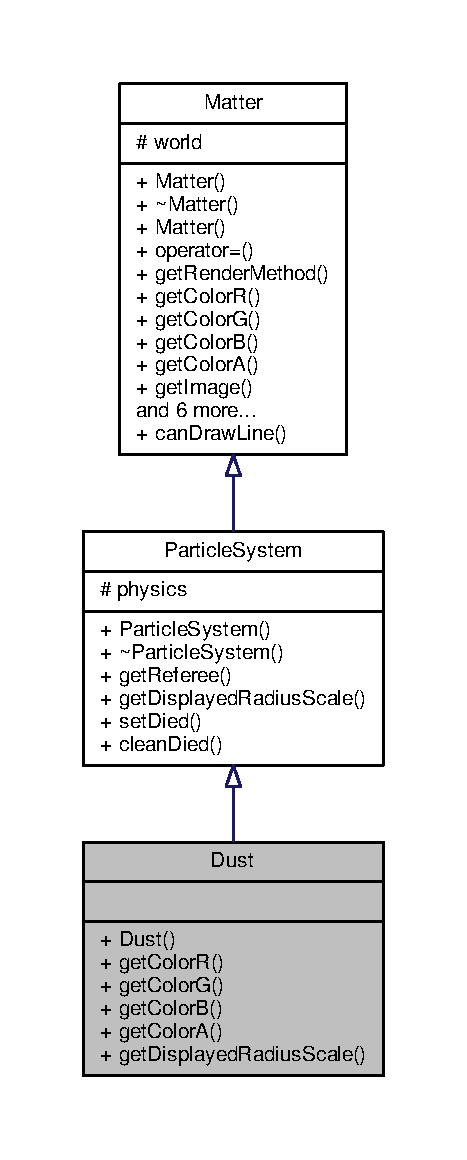
\includegraphics[height=550pt]{classDust__inherit__graph}
\end{center}
\end{figure}


Collaboration diagram for Dust\+:
\nopagebreak
\begin{figure}[H]
\begin{center}
\leavevmode
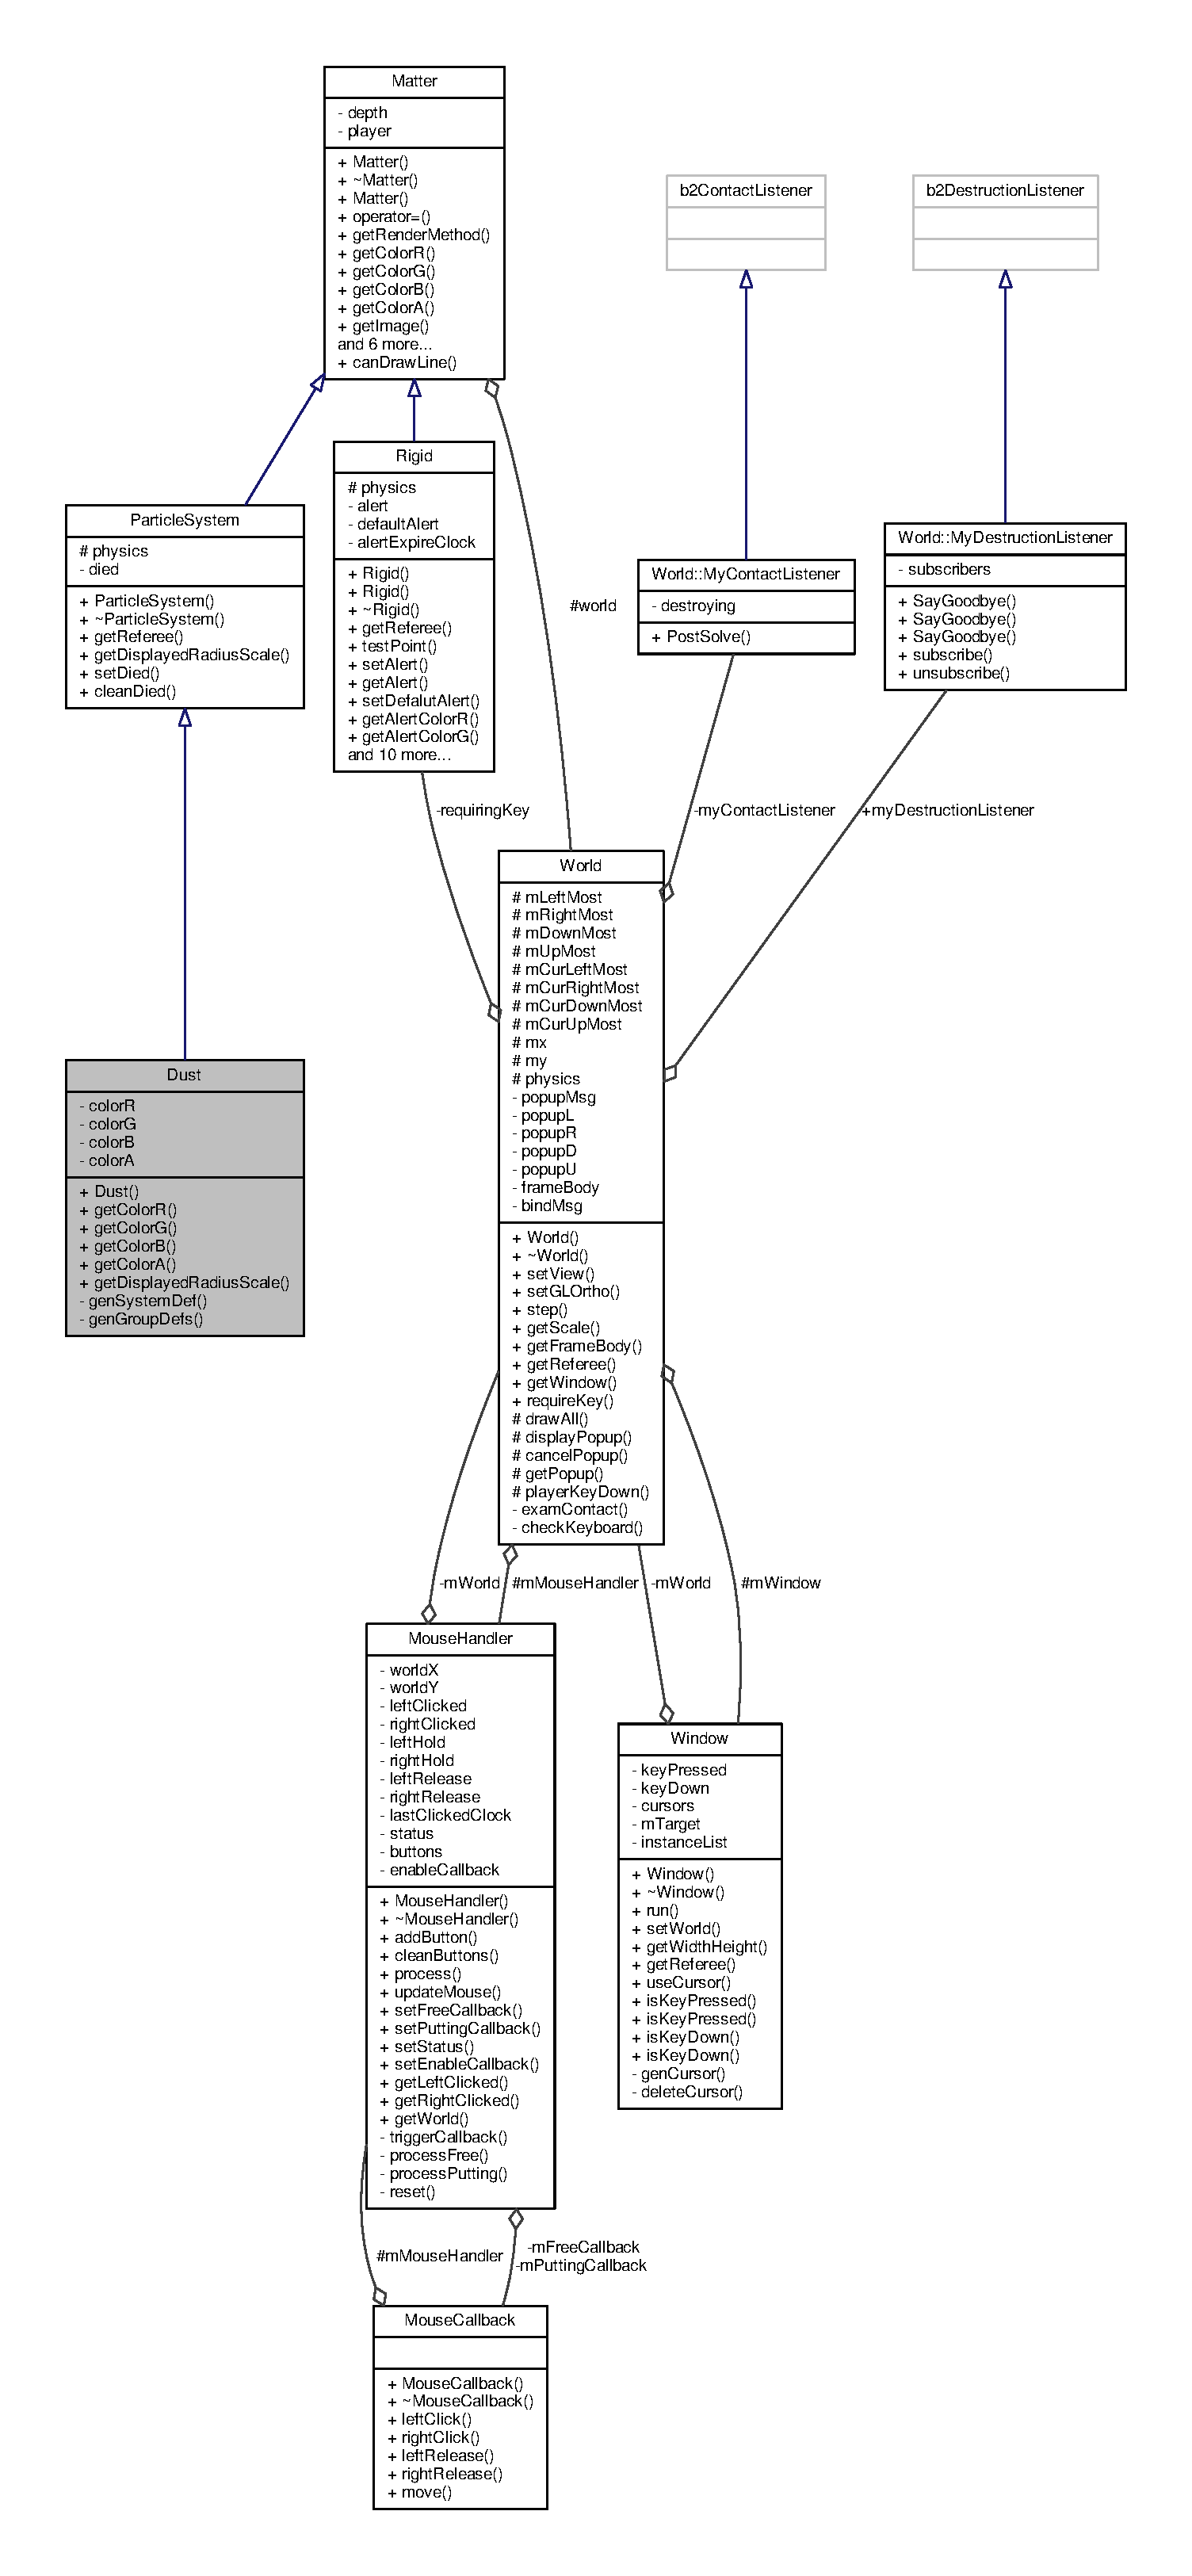
\includegraphics[height=550pt]{classDust__coll__graph}
\end{center}
\end{figure}
\subsection*{Public Member Functions}
\begin{DoxyCompactItemize}
\item 
\hyperlink{classDust_a43719fa4b8745b2bd2eb72f2590786c2}{Dust} (\hyperlink{classWorld}{World} $\ast$\+\_\+world, const b2\+Vec2 \&pos, const std\+::vector$<$ b2\+Shape $\ast$ $>$ \&shapes, const b2\+Vec2 \&v, float w, float \+\_\+color\+R, float \+\_\+color\+G, float \+\_\+color\+B, float \+\_\+color\+A) noexcept
\item 
virtual float \hyperlink{classDust_a2e5d596ac110553eb401eae59641fb5a}{get\+Color\+R} () const override
\item 
virtual float \hyperlink{classDust_a386313dcd344747fb28bb809f6243bf8}{get\+Color\+G} () const override
\item 
virtual float \hyperlink{classDust_a088431d5f6a114d93f12cae63592a8dd}{get\+Color\+B} () const override
\item 
virtual float \hyperlink{classDust_a6a61ed84ae1cbba8d0cdbc102a343f0f}{get\+Color\+A} () const override
\item 
virtual float \hyperlink{classDust_a6e96475d0b48ffcfb443c014ad369276}{get\+Displayed\+Radius\+Scale} () const override
\begin{DoxyCompactList}\small\item\em displayed radius = ? $\ast$ physics radius \end{DoxyCompactList}\end{DoxyCompactItemize}
\subsection*{Static Private Member Functions}
\begin{DoxyCompactItemize}
\item 
static b2\+Particle\+System\+Def \hyperlink{classDust_a91cc6bf0a6060b14fa4e21759f3581c8}{gen\+System\+Def} ()
\item 
static std\+::vector$<$ b2\+Particle\+Group\+Def $>$ \hyperlink{classDust_a13883a1eaaf0e0e07529060dca61f6c9}{gen\+Group\+Defs} (const b2\+Vec2 \&pos, const std\+::vector$<$ b2\+Shape $\ast$ $>$ \&shapes, const b2\+Vec2 \&v, float w, float \+\_\+color\+R, float \+\_\+color\+G, float \+\_\+color\+B, float \+\_\+color\+A)
\end{DoxyCompactItemize}
\subsection*{Private Attributes}
\begin{DoxyCompactItemize}
\item 
float \hyperlink{classDust_a38fced9e145e03d4bb548924bd99a7fd}{color\+R}
\item 
float \hyperlink{classDust_a97d9fa2655101d2ea41c1a6a5f89bd32}{color\+G}
\item 
float \hyperlink{classDust_a3c3ad4aa31b2d0220cab1569743bb836}{color\+B}
\item 
float \hyperlink{classDust_aa726a6672b4777821df8efaa789549a3}{color\+A}
\end{DoxyCompactItemize}
\subsection*{Additional Inherited Members}


\subsection{Detailed Description}
\hyperlink{classDust}{Dust} rised when a rigid is damaged. 

\subsection{Constructor \& Destructor Documentation}
\hypertarget{classDust_a43719fa4b8745b2bd2eb72f2590786c2}{}\index{Dust@{Dust}!Dust@{Dust}}
\index{Dust@{Dust}!Dust@{Dust}}
\subsubsection[{Dust}]{\setlength{\rightskip}{0pt plus 5cm}Dust\+::\+Dust (
\begin{DoxyParamCaption}
\item[{{\bf World} $\ast$}]{\+\_\+world, }
\item[{const b2\+Vec2 \&}]{pos, }
\item[{const std\+::vector$<$ b2\+Shape $\ast$ $>$ \&}]{shapes, }
\item[{const b2\+Vec2 \&}]{v, }
\item[{float}]{w, }
\item[{float}]{\+\_\+color\+R, }
\item[{float}]{\+\_\+color\+G, }
\item[{float}]{\+\_\+color\+B, }
\item[{float}]{\+\_\+color\+A}
\end{DoxyParamCaption}
)\hspace{0.3cm}{\ttfamily [noexcept]}}\label{classDust_a43719fa4b8745b2bd2eb72f2590786c2}

\begin{DoxyParams}{Parameters}
{\em v} & \+: linear velocity \\
\hline
{\em w} & \+: angular velocity \\
\hline
\end{DoxyParams}


\subsection{Member Function Documentation}
\hypertarget{classDust_a13883a1eaaf0e0e07529060dca61f6c9}{}\index{Dust@{Dust}!gen\+Group\+Defs@{gen\+Group\+Defs}}
\index{gen\+Group\+Defs@{gen\+Group\+Defs}!Dust@{Dust}}
\subsubsection[{gen\+Group\+Defs}]{\setlength{\rightskip}{0pt plus 5cm}std\+::vector$<$ b2\+Particle\+Group\+Def $>$ Dust\+::gen\+Group\+Defs (
\begin{DoxyParamCaption}
\item[{const b2\+Vec2 \&}]{pos, }
\item[{const std\+::vector$<$ b2\+Shape $\ast$ $>$ \&}]{shapes, }
\item[{const b2\+Vec2 \&}]{v, }
\item[{float}]{w, }
\item[{float}]{\+\_\+color\+R, }
\item[{float}]{\+\_\+color\+G, }
\item[{float}]{\+\_\+color\+B, }
\item[{float}]{\+\_\+color\+A}
\end{DoxyParamCaption}
)\hspace{0.3cm}{\ttfamily [static]}, {\ttfamily [private]}}\label{classDust_a13883a1eaaf0e0e07529060dca61f6c9}
\hypertarget{classDust_a91cc6bf0a6060b14fa4e21759f3581c8}{}\index{Dust@{Dust}!gen\+System\+Def@{gen\+System\+Def}}
\index{gen\+System\+Def@{gen\+System\+Def}!Dust@{Dust}}
\subsubsection[{gen\+System\+Def}]{\setlength{\rightskip}{0pt plus 5cm}b2\+Particle\+System\+Def Dust\+::gen\+System\+Def (
\begin{DoxyParamCaption}
{}
\end{DoxyParamCaption}
)\hspace{0.3cm}{\ttfamily [static]}, {\ttfamily [private]}}\label{classDust_a91cc6bf0a6060b14fa4e21759f3581c8}
\hypertarget{classDust_a6a61ed84ae1cbba8d0cdbc102a343f0f}{}\index{Dust@{Dust}!get\+Color\+A@{get\+Color\+A}}
\index{get\+Color\+A@{get\+Color\+A}!Dust@{Dust}}
\subsubsection[{get\+Color\+A}]{\setlength{\rightskip}{0pt plus 5cm}virtual float Dust\+::get\+Color\+A (
\begin{DoxyParamCaption}
{}
\end{DoxyParamCaption}
) const\hspace{0.3cm}{\ttfamily [inline]}, {\ttfamily [override]}, {\ttfamily [virtual]}}\label{classDust_a6a61ed84ae1cbba8d0cdbc102a343f0f}


Reimplemented from \hyperlink{classMatter_aa44ee7ba48cb9a582a6f86e1e9e2ef38}{Matter}.

\hypertarget{classDust_a088431d5f6a114d93f12cae63592a8dd}{}\index{Dust@{Dust}!get\+Color\+B@{get\+Color\+B}}
\index{get\+Color\+B@{get\+Color\+B}!Dust@{Dust}}
\subsubsection[{get\+Color\+B}]{\setlength{\rightskip}{0pt plus 5cm}virtual float Dust\+::get\+Color\+B (
\begin{DoxyParamCaption}
{}
\end{DoxyParamCaption}
) const\hspace{0.3cm}{\ttfamily [inline]}, {\ttfamily [override]}, {\ttfamily [virtual]}}\label{classDust_a088431d5f6a114d93f12cae63592a8dd}


Reimplemented from \hyperlink{classMatter_af830da17da427c84c7f6deee4a91b3d4}{Matter}.

\hypertarget{classDust_a386313dcd344747fb28bb809f6243bf8}{}\index{Dust@{Dust}!get\+Color\+G@{get\+Color\+G}}
\index{get\+Color\+G@{get\+Color\+G}!Dust@{Dust}}
\subsubsection[{get\+Color\+G}]{\setlength{\rightskip}{0pt plus 5cm}virtual float Dust\+::get\+Color\+G (
\begin{DoxyParamCaption}
{}
\end{DoxyParamCaption}
) const\hspace{0.3cm}{\ttfamily [inline]}, {\ttfamily [override]}, {\ttfamily [virtual]}}\label{classDust_a386313dcd344747fb28bb809f6243bf8}


Reimplemented from \hyperlink{classMatter_aa3fcdc82f788fbf873ec3ff4808f614a}{Matter}.

\hypertarget{classDust_a2e5d596ac110553eb401eae59641fb5a}{}\index{Dust@{Dust}!get\+Color\+R@{get\+Color\+R}}
\index{get\+Color\+R@{get\+Color\+R}!Dust@{Dust}}
\subsubsection[{get\+Color\+R}]{\setlength{\rightskip}{0pt plus 5cm}virtual float Dust\+::get\+Color\+R (
\begin{DoxyParamCaption}
{}
\end{DoxyParamCaption}
) const\hspace{0.3cm}{\ttfamily [inline]}, {\ttfamily [override]}, {\ttfamily [virtual]}}\label{classDust_a2e5d596ac110553eb401eae59641fb5a}


Reimplemented from \hyperlink{classMatter_a926d246584228c3e3b102dbfd42036ec}{Matter}.

\hypertarget{classDust_a6e96475d0b48ffcfb443c014ad369276}{}\index{Dust@{Dust}!get\+Displayed\+Radius\+Scale@{get\+Displayed\+Radius\+Scale}}
\index{get\+Displayed\+Radius\+Scale@{get\+Displayed\+Radius\+Scale}!Dust@{Dust}}
\subsubsection[{get\+Displayed\+Radius\+Scale}]{\setlength{\rightskip}{0pt plus 5cm}virtual float Dust\+::get\+Displayed\+Radius\+Scale (
\begin{DoxyParamCaption}
{}
\end{DoxyParamCaption}
) const\hspace{0.3cm}{\ttfamily [inline]}, {\ttfamily [override]}, {\ttfamily [virtual]}}\label{classDust_a6e96475d0b48ffcfb443c014ad369276}


displayed radius = ? $\ast$ physics radius 



Implements \hyperlink{classParticleSystem_a5b3bcfbc82de5d335f55173b049da517}{Particle\+System}.



\subsection{Member Data Documentation}
\hypertarget{classDust_aa726a6672b4777821df8efaa789549a3}{}\index{Dust@{Dust}!color\+A@{color\+A}}
\index{color\+A@{color\+A}!Dust@{Dust}}
\subsubsection[{color\+A}]{\setlength{\rightskip}{0pt plus 5cm}float Dust\+::color\+A\hspace{0.3cm}{\ttfamily [private]}}\label{classDust_aa726a6672b4777821df8efaa789549a3}
\hypertarget{classDust_a3c3ad4aa31b2d0220cab1569743bb836}{}\index{Dust@{Dust}!color\+B@{color\+B}}
\index{color\+B@{color\+B}!Dust@{Dust}}
\subsubsection[{color\+B}]{\setlength{\rightskip}{0pt plus 5cm}float Dust\+::color\+B\hspace{0.3cm}{\ttfamily [private]}}\label{classDust_a3c3ad4aa31b2d0220cab1569743bb836}
\hypertarget{classDust_a97d9fa2655101d2ea41c1a6a5f89bd32}{}\index{Dust@{Dust}!color\+G@{color\+G}}
\index{color\+G@{color\+G}!Dust@{Dust}}
\subsubsection[{color\+G}]{\setlength{\rightskip}{0pt plus 5cm}float Dust\+::color\+G\hspace{0.3cm}{\ttfamily [private]}}\label{classDust_a97d9fa2655101d2ea41c1a6a5f89bd32}
\hypertarget{classDust_a38fced9e145e03d4bb548924bd99a7fd}{}\index{Dust@{Dust}!color\+R@{color\+R}}
\index{color\+R@{color\+R}!Dust@{Dust}}
\subsubsection[{color\+R}]{\setlength{\rightskip}{0pt plus 5cm}float Dust\+::color\+R\hspace{0.3cm}{\ttfamily [private]}}\label{classDust_a38fced9e145e03d4bb548924bd99a7fd}


The documentation for this class was generated from the following files\+:\begin{DoxyCompactItemize}
\item 
\hyperlink{matter_8h}{matter.\+h}\item 
\hyperlink{matter_8cpp}{matter.\+cpp}\end{DoxyCompactItemize}

\hypertarget{classEnemy}{}\section{Enemy Class Reference}
\label{classEnemy}\index{Enemy@{Enemy}}


This class loads and controls enemy.  




{\ttfamily \#include $<$enemy.\+h$>$}



Collaboration diagram for Enemy\+:\nopagebreak
\begin{figure}[H]
\begin{center}
\leavevmode
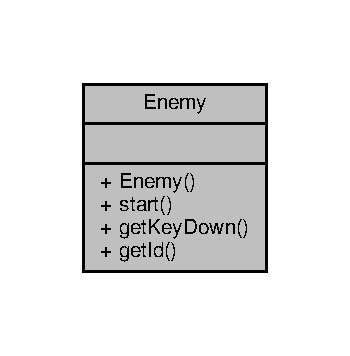
\includegraphics[width=168pt]{classEnemy__coll__graph}
\end{center}
\end{figure}
\subsection*{Public Member Functions}
\begin{DoxyCompactItemize}
\item 
\hyperlink{classEnemy_a05371b05fdaf447e2811a74e64dd3cf5}{Enemy} (\hyperlink{classWorld}{World} $\ast$world, std\+::vector$<$ std\+::string $>$ \+\_\+path, float \+\_\+offset\+X)
\item 
void \hyperlink{classEnemy_a71641016b8ea6de06deeda6926600da8}{start} ()
\begin{DoxyCompactList}\small\item\em set objects to the world \end{DoxyCompactList}\item 
bool \hyperlink{classEnemy_ac96f56669570d7acf7d53cf21e13b639}{get\+Key\+Down} (int key)
\begin{DoxyCompactList}\small\item\em if key down now? \end{DoxyCompactList}\item 
int \hyperlink{classEnemy_ad24d8afab5f4f150d7bb87ec96baf84d}{get\+Id} () const 
\end{DoxyCompactItemize}


\subsection{Detailed Description}
This class loads and controls enemy. 

\subsection{Constructor \& Destructor Documentation}
\hypertarget{classEnemy_a05371b05fdaf447e2811a74e64dd3cf5}{}\index{Enemy@{Enemy}!Enemy@{Enemy}}
\index{Enemy@{Enemy}!Enemy@{Enemy}}
\subsubsection[{Enemy}]{\setlength{\rightskip}{0pt plus 5cm}Enemy\+::\+Enemy (
\begin{DoxyParamCaption}
\item[{{\bf World} $\ast$}]{world, }
\item[{std\+::vector$<$ std\+::string $>$}]{\+\_\+path, }
\item[{float}]{\+\_\+offset\+X}
\end{DoxyParamCaption}
)}\label{classEnemy_a05371b05fdaf447e2811a74e64dd3cf5}


\subsection{Member Function Documentation}
\hypertarget{classEnemy_ad24d8afab5f4f150d7bb87ec96baf84d}{}\index{Enemy@{Enemy}!get\+Id@{get\+Id}}
\index{get\+Id@{get\+Id}!Enemy@{Enemy}}
\subsubsection[{get\+Id}]{\setlength{\rightskip}{0pt plus 5cm}int Enemy\+::get\+Id (
\begin{DoxyParamCaption}
{}
\end{DoxyParamCaption}
) const\hspace{0.3cm}{\ttfamily [inline]}}\label{classEnemy_ad24d8afab5f4f150d7bb87ec96baf84d}
\hypertarget{classEnemy_ac96f56669570d7acf7d53cf21e13b639}{}\index{Enemy@{Enemy}!get\+Key\+Down@{get\+Key\+Down}}
\index{get\+Key\+Down@{get\+Key\+Down}!Enemy@{Enemy}}
\subsubsection[{get\+Key\+Down}]{\setlength{\rightskip}{0pt plus 5cm}bool Enemy\+::get\+Key\+Down (
\begin{DoxyParamCaption}
\item[{int}]{key}
\end{DoxyParamCaption}
)}\label{classEnemy_ac96f56669570d7acf7d53cf21e13b639}


if key down now? 

\hypertarget{classEnemy_a71641016b8ea6de06deeda6926600da8}{}\index{Enemy@{Enemy}!start@{start}}
\index{start@{start}!Enemy@{Enemy}}
\subsubsection[{start}]{\setlength{\rightskip}{0pt plus 5cm}void Enemy\+::start (
\begin{DoxyParamCaption}
{}
\end{DoxyParamCaption}
)}\label{classEnemy_a71641016b8ea6de06deeda6926600da8}


set objects to the world 



The documentation for this class was generated from the following files\+:\begin{DoxyCompactItemize}
\item 
\hyperlink{enemy_8h}{enemy.\+h}\item 
\hyperlink{enemy_8cpp}{enemy.\+cpp}\end{DoxyCompactItemize}

\hypertarget{classEngine}{}\section{Engine Class Reference}
\label{classEngine}\index{Engine@{Engine}}


Base class of engines.  




{\ttfamily \#include $<$matter.\+h$>$}



Inheritance diagram for Engine\+:
\nopagebreak
\begin{figure}[H]
\begin{center}
\leavevmode
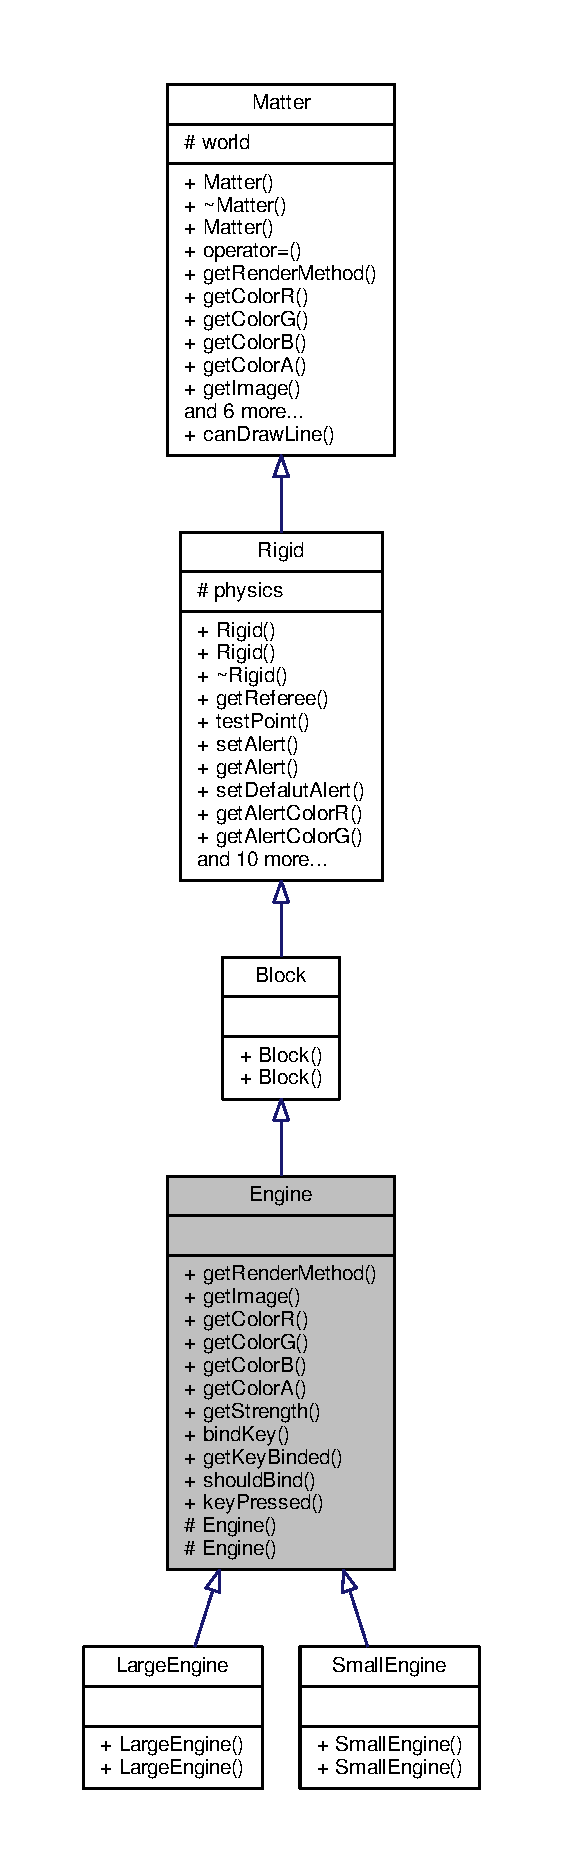
\includegraphics[height=550pt]{classEngine__inherit__graph}
\end{center}
\end{figure}


Collaboration diagram for Engine\+:
\nopagebreak
\begin{figure}[H]
\begin{center}
\leavevmode
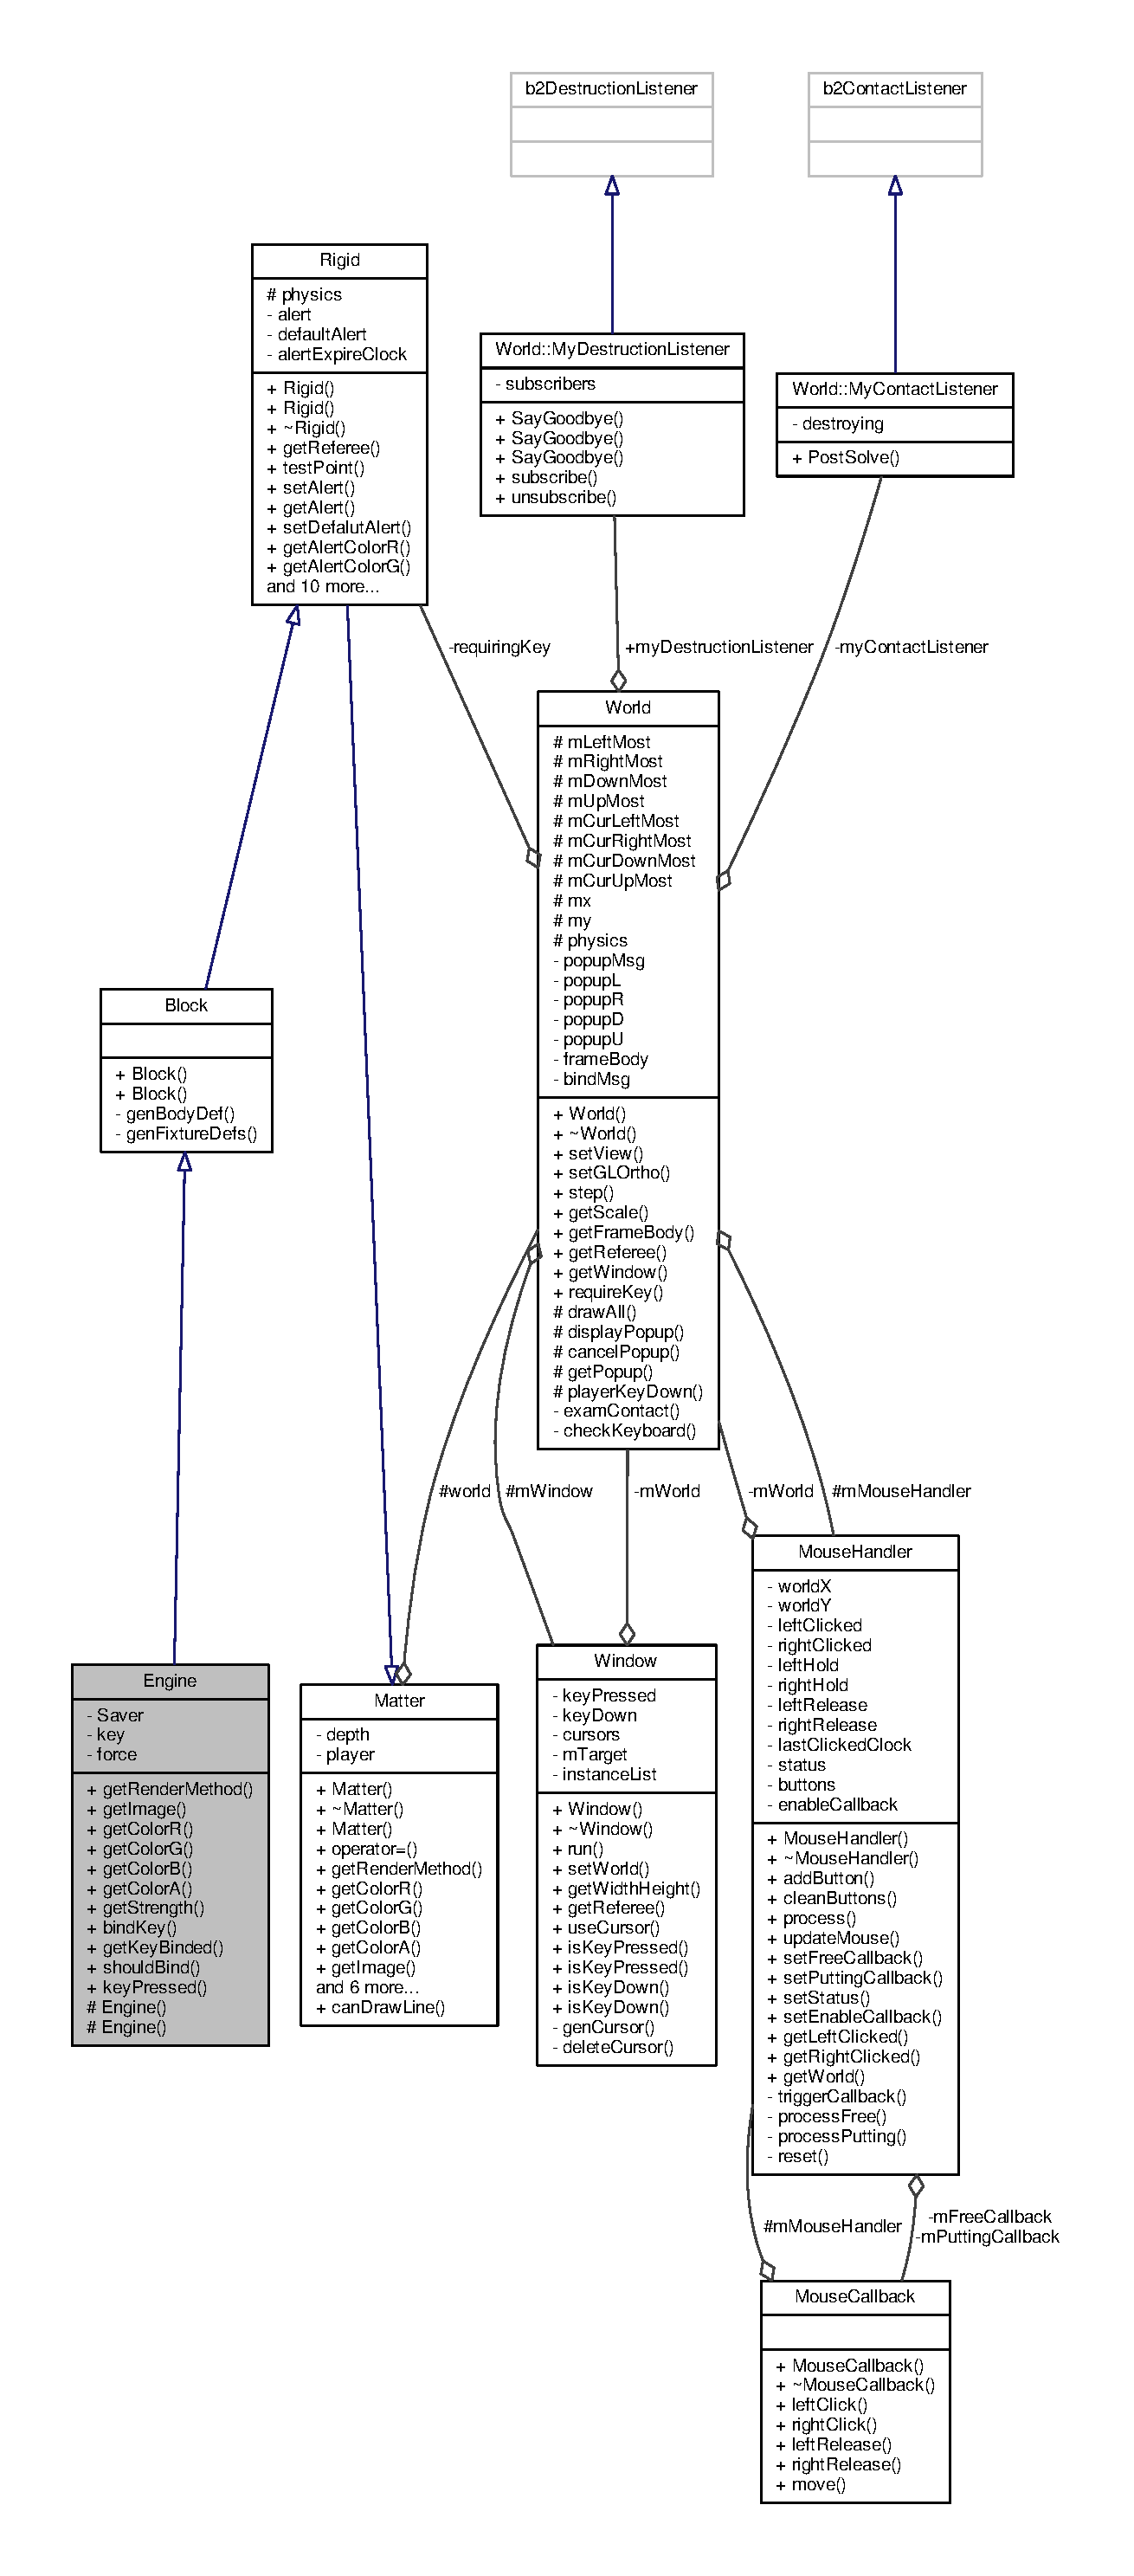
\includegraphics[height=550pt]{classEngine__coll__graph}
\end{center}
\end{figure}
\subsection*{Public Member Functions}
\begin{DoxyCompactItemize}
\item 
virtual \hyperlink{classMatter_ade1ce1bf81f25377f689d103cd431907}{Render\+Method} \hyperlink{classEngine_a72c7a3ea05ac92bdb909e11b20d8d6fc}{get\+Render\+Method} () const override
\item 
virtual \hyperlink{image_8h_af9361b398b5cfcafbe93f82e8eaeb080}{Image\+Name} \hyperlink{classEngine_a130b5e67a05c2ea6f9c2f5d7a4fc60dd}{get\+Image} () const override
\item 
virtual float \hyperlink{classEngine_a9ad7ea816b850dc812b6a792493a803e}{get\+Color\+R} () const override
\item 
virtual float \hyperlink{classEngine_abd2e81839210c4c98b6cad705af25cec}{get\+Color\+G} () const override
\item 
virtual float \hyperlink{classEngine_aefc235452646da3c6b9b77c625ef3278}{get\+Color\+B} () const override
\item 
virtual float \hyperlink{classEngine_aefe56a242ce462d18958c2e217a0df7a}{get\+Color\+A} () const override
\item 
virtual float \hyperlink{classEngine_a1cf8f75f0ccc44aee67aea3174cee308}{get\+Strength} () const override
\begin{DoxyCompactList}\small\item\em rigids are undestroyable by default \end{DoxyCompactList}\item 
void \hyperlink{classEngine_adcebb4115667ea0924af3b5aeb5fd5e2}{bind\+Key} (int \+\_\+key) override
\begin{DoxyCompactList}\small\item\em bind a key on the keyboard to control it 0 = none \end{DoxyCompactList}\item 
int \hyperlink{classEngine_afedd663b3ada7e15028fd157be3f4517}{get\+Key\+Binded} () const override
\begin{DoxyCompactList}\small\item\em what has it bind? \end{DoxyCompactList}\item 
bool \hyperlink{classEngine_a5f949b7b1d1c621de8940470adbc3901}{should\+Bind} () const override
\begin{DoxyCompactList}\small\item\em shoud we bind a key to it? \end{DoxyCompactList}\item 
void \hyperlink{classEngine_a7ec1e7e83a96a39490bc13b6906250f3}{key\+Pressed} () override
\begin{DoxyCompactList}\small\item\em what should it do when the key above is pressed \end{DoxyCompactList}\end{DoxyCompactItemize}
\subsection*{Protected Member Functions}
\begin{DoxyCompactItemize}
\item 
\hyperlink{classEngine_aa51d8d3d86d7cf49b9e09783021d185f}{Engine} (\hyperlink{classWorld}{World} $\ast$\+\_\+world, b2\+Body $\ast$\hyperlink{image_8h_ab2d05693952610f937e5acb3c4a8fa1b}{b}, float \+\_\+force)
\item 
\hyperlink{classEngine_a527eb3c0df224d20081ca4b2f84c2023}{Engine} (\hyperlink{classWorld}{World} $\ast$\+\_\+world, float x, float y, float w, float h, float \+\_\+force) noexcept
\end{DoxyCompactItemize}
\subsection*{Private Attributes}
\begin{DoxyCompactItemize}
\item 
friend \hyperlink{classEngine_aab36737a1fbe9e5ec464118849615d35}{Saver}
\item 
int \hyperlink{classEngine_a134558741b3eb55f716b1ca177a095d6}{key}
\item 
float \hyperlink{classEngine_aecd30a2b62a3c3d969f5d57892c1c131}{force}
\end{DoxyCompactItemize}
\subsection*{Additional Inherited Members}


\subsection{Detailed Description}
Base class of engines. 

\subsection{Constructor \& Destructor Documentation}
\hypertarget{classEngine_aa51d8d3d86d7cf49b9e09783021d185f}{}\index{Engine@{Engine}!Engine@{Engine}}
\index{Engine@{Engine}!Engine@{Engine}}
\subsubsection[{Engine}]{\setlength{\rightskip}{0pt plus 5cm}Engine\+::\+Engine (
\begin{DoxyParamCaption}
\item[{{\bf World} $\ast$}]{\+\_\+world, }
\item[{b2\+Body $\ast$}]{b, }
\item[{float}]{\+\_\+force}
\end{DoxyParamCaption}
)\hspace{0.3cm}{\ttfamily [inline]}, {\ttfamily [protected]}}\label{classEngine_aa51d8d3d86d7cf49b9e09783021d185f}
\hypertarget{classEngine_a527eb3c0df224d20081ca4b2f84c2023}{}\index{Engine@{Engine}!Engine@{Engine}}
\index{Engine@{Engine}!Engine@{Engine}}
\subsubsection[{Engine}]{\setlength{\rightskip}{0pt plus 5cm}Engine\+::\+Engine (
\begin{DoxyParamCaption}
\item[{{\bf World} $\ast$}]{\+\_\+world, }
\item[{float}]{x, }
\item[{float}]{y, }
\item[{float}]{w, }
\item[{float}]{h, }
\item[{float}]{\+\_\+force}
\end{DoxyParamCaption}
)\hspace{0.3cm}{\ttfamily [protected]}, {\ttfamily [noexcept]}}\label{classEngine_a527eb3c0df224d20081ca4b2f84c2023}


\subsection{Member Function Documentation}
\hypertarget{classEngine_adcebb4115667ea0924af3b5aeb5fd5e2}{}\index{Engine@{Engine}!bind\+Key@{bind\+Key}}
\index{bind\+Key@{bind\+Key}!Engine@{Engine}}
\subsubsection[{bind\+Key}]{\setlength{\rightskip}{0pt plus 5cm}void Engine\+::bind\+Key (
\begin{DoxyParamCaption}
\item[{int}]{\+\_\+key}
\end{DoxyParamCaption}
)\hspace{0.3cm}{\ttfamily [inline]}, {\ttfamily [override]}, {\ttfamily [virtual]}}\label{classEngine_adcebb4115667ea0924af3b5aeb5fd5e2}


bind a key on the keyboard to control it 0 = none 



Reimplemented from \hyperlink{classRigid_a5d8922b10420ad452b6d9400d5ecc511}{Rigid}.

\hypertarget{classEngine_aefe56a242ce462d18958c2e217a0df7a}{}\index{Engine@{Engine}!get\+Color\+A@{get\+Color\+A}}
\index{get\+Color\+A@{get\+Color\+A}!Engine@{Engine}}
\subsubsection[{get\+Color\+A}]{\setlength{\rightskip}{0pt plus 5cm}virtual float Engine\+::get\+Color\+A (
\begin{DoxyParamCaption}
{}
\end{DoxyParamCaption}
) const\hspace{0.3cm}{\ttfamily [inline]}, {\ttfamily [override]}, {\ttfamily [virtual]}}\label{classEngine_aefe56a242ce462d18958c2e217a0df7a}


Reimplemented from \hyperlink{classMatter_aa44ee7ba48cb9a582a6f86e1e9e2ef38}{Matter}.

\hypertarget{classEngine_aefc235452646da3c6b9b77c625ef3278}{}\index{Engine@{Engine}!get\+Color\+B@{get\+Color\+B}}
\index{get\+Color\+B@{get\+Color\+B}!Engine@{Engine}}
\subsubsection[{get\+Color\+B}]{\setlength{\rightskip}{0pt plus 5cm}virtual float Engine\+::get\+Color\+B (
\begin{DoxyParamCaption}
{}
\end{DoxyParamCaption}
) const\hspace{0.3cm}{\ttfamily [inline]}, {\ttfamily [override]}, {\ttfamily [virtual]}}\label{classEngine_aefc235452646da3c6b9b77c625ef3278}


Reimplemented from \hyperlink{classMatter_af830da17da427c84c7f6deee4a91b3d4}{Matter}.

\hypertarget{classEngine_abd2e81839210c4c98b6cad705af25cec}{}\index{Engine@{Engine}!get\+Color\+G@{get\+Color\+G}}
\index{get\+Color\+G@{get\+Color\+G}!Engine@{Engine}}
\subsubsection[{get\+Color\+G}]{\setlength{\rightskip}{0pt plus 5cm}virtual float Engine\+::get\+Color\+G (
\begin{DoxyParamCaption}
{}
\end{DoxyParamCaption}
) const\hspace{0.3cm}{\ttfamily [inline]}, {\ttfamily [override]}, {\ttfamily [virtual]}}\label{classEngine_abd2e81839210c4c98b6cad705af25cec}


Reimplemented from \hyperlink{classMatter_aa3fcdc82f788fbf873ec3ff4808f614a}{Matter}.

\hypertarget{classEngine_a9ad7ea816b850dc812b6a792493a803e}{}\index{Engine@{Engine}!get\+Color\+R@{get\+Color\+R}}
\index{get\+Color\+R@{get\+Color\+R}!Engine@{Engine}}
\subsubsection[{get\+Color\+R}]{\setlength{\rightskip}{0pt plus 5cm}virtual float Engine\+::get\+Color\+R (
\begin{DoxyParamCaption}
{}
\end{DoxyParamCaption}
) const\hspace{0.3cm}{\ttfamily [inline]}, {\ttfamily [override]}, {\ttfamily [virtual]}}\label{classEngine_a9ad7ea816b850dc812b6a792493a803e}


Reimplemented from \hyperlink{classMatter_a926d246584228c3e3b102dbfd42036ec}{Matter}.

\hypertarget{classEngine_a130b5e67a05c2ea6f9c2f5d7a4fc60dd}{}\index{Engine@{Engine}!get\+Image@{get\+Image}}
\index{get\+Image@{get\+Image}!Engine@{Engine}}
\subsubsection[{get\+Image}]{\setlength{\rightskip}{0pt plus 5cm}virtual {\bf Image\+Name} Engine\+::get\+Image (
\begin{DoxyParamCaption}
{}
\end{DoxyParamCaption}
) const\hspace{0.3cm}{\ttfamily [inline]}, {\ttfamily [override]}, {\ttfamily [virtual]}}\label{classEngine_a130b5e67a05c2ea6f9c2f5d7a4fc60dd}


Reimplemented from \hyperlink{classMatter_ad6202a62e4ae27dde457c56520f1865e}{Matter}.

\hypertarget{classEngine_afedd663b3ada7e15028fd157be3f4517}{}\index{Engine@{Engine}!get\+Key\+Binded@{get\+Key\+Binded}}
\index{get\+Key\+Binded@{get\+Key\+Binded}!Engine@{Engine}}
\subsubsection[{get\+Key\+Binded}]{\setlength{\rightskip}{0pt plus 5cm}int Engine\+::get\+Key\+Binded (
\begin{DoxyParamCaption}
{}
\end{DoxyParamCaption}
) const\hspace{0.3cm}{\ttfamily [inline]}, {\ttfamily [override]}, {\ttfamily [virtual]}}\label{classEngine_afedd663b3ada7e15028fd157be3f4517}


what has it bind? 



Reimplemented from \hyperlink{classRigid_a4e5382b25c00ff97745b04120e51cb56}{Rigid}.

\hypertarget{classEngine_a72c7a3ea05ac92bdb909e11b20d8d6fc}{}\index{Engine@{Engine}!get\+Render\+Method@{get\+Render\+Method}}
\index{get\+Render\+Method@{get\+Render\+Method}!Engine@{Engine}}
\subsubsection[{get\+Render\+Method}]{\setlength{\rightskip}{0pt plus 5cm}virtual {\bf Render\+Method} Engine\+::get\+Render\+Method (
\begin{DoxyParamCaption}
{}
\end{DoxyParamCaption}
) const\hspace{0.3cm}{\ttfamily [inline]}, {\ttfamily [override]}, {\ttfamily [virtual]}}\label{classEngine_a72c7a3ea05ac92bdb909e11b20d8d6fc}


Reimplemented from \hyperlink{classMatter_a3d6823a375fe0a537837b905b44af5bd}{Matter}.

\hypertarget{classEngine_a1cf8f75f0ccc44aee67aea3174cee308}{}\index{Engine@{Engine}!get\+Strength@{get\+Strength}}
\index{get\+Strength@{get\+Strength}!Engine@{Engine}}
\subsubsection[{get\+Strength}]{\setlength{\rightskip}{0pt plus 5cm}virtual float Engine\+::get\+Strength (
\begin{DoxyParamCaption}
{}
\end{DoxyParamCaption}
) const\hspace{0.3cm}{\ttfamily [inline]}, {\ttfamily [override]}, {\ttfamily [virtual]}}\label{classEngine_a1cf8f75f0ccc44aee67aea3174cee308}


rigids are undestroyable by default 



Reimplemented from \hyperlink{classRigid_aac83bf941605a8cbccf06a5d4b200fee}{Rigid}.

\hypertarget{classEngine_a7ec1e7e83a96a39490bc13b6906250f3}{}\index{Engine@{Engine}!key\+Pressed@{key\+Pressed}}
\index{key\+Pressed@{key\+Pressed}!Engine@{Engine}}
\subsubsection[{key\+Pressed}]{\setlength{\rightskip}{0pt plus 5cm}void Engine\+::key\+Pressed (
\begin{DoxyParamCaption}
{}
\end{DoxyParamCaption}
)\hspace{0.3cm}{\ttfamily [override]}, {\ttfamily [virtual]}}\label{classEngine_a7ec1e7e83a96a39490bc13b6906250f3}


what should it do when the key above is pressed 



Reimplemented from \hyperlink{classRigid_a769957138e3ca40a4a6b1da4cf52eea8}{Rigid}.

\hypertarget{classEngine_a5f949b7b1d1c621de8940470adbc3901}{}\index{Engine@{Engine}!should\+Bind@{should\+Bind}}
\index{should\+Bind@{should\+Bind}!Engine@{Engine}}
\subsubsection[{should\+Bind}]{\setlength{\rightskip}{0pt plus 5cm}bool Engine\+::should\+Bind (
\begin{DoxyParamCaption}
{}
\end{DoxyParamCaption}
) const\hspace{0.3cm}{\ttfamily [inline]}, {\ttfamily [override]}, {\ttfamily [virtual]}}\label{classEngine_a5f949b7b1d1c621de8940470adbc3901}


shoud we bind a key to it? 



Reimplemented from \hyperlink{classRigid_a213d4ddd819ea799b7a29961b0d66f39}{Rigid}.



\subsection{Member Data Documentation}
\hypertarget{classEngine_aecd30a2b62a3c3d969f5d57892c1c131}{}\index{Engine@{Engine}!force@{force}}
\index{force@{force}!Engine@{Engine}}
\subsubsection[{force}]{\setlength{\rightskip}{0pt plus 5cm}float Engine\+::force\hspace{0.3cm}{\ttfamily [private]}}\label{classEngine_aecd30a2b62a3c3d969f5d57892c1c131}
\hypertarget{classEngine_a134558741b3eb55f716b1ca177a095d6}{}\index{Engine@{Engine}!key@{key}}
\index{key@{key}!Engine@{Engine}}
\subsubsection[{key}]{\setlength{\rightskip}{0pt plus 5cm}int Engine\+::key\hspace{0.3cm}{\ttfamily [private]}}\label{classEngine_a134558741b3eb55f716b1ca177a095d6}
\hypertarget{classEngine_aab36737a1fbe9e5ec464118849615d35}{}\index{Engine@{Engine}!Saver@{Saver}}
\index{Saver@{Saver}!Engine@{Engine}}
\subsubsection[{Saver}]{\setlength{\rightskip}{0pt plus 5cm}friend Engine\+::\+Saver\hspace{0.3cm}{\ttfamily [private]}}\label{classEngine_aab36737a1fbe9e5ec464118849615d35}


The documentation for this class was generated from the following files\+:\begin{DoxyCompactItemize}
\item 
\hyperlink{matter_8h}{matter.\+h}\item 
\hyperlink{matter_8cpp}{matter.\+cpp}\end{DoxyCompactItemize}

\hypertarget{classRender_1_1FixtureRenderer}{}\section{Render\+:\+:Fixture\+Renderer Class Reference}
\label{classRender_1_1FixtureRenderer}\index{Render\+::\+Fixture\+Renderer@{Render\+::\+Fixture\+Renderer}}


Inheritance diagram for Render\+:\+:Fixture\+Renderer\+:
\nopagebreak
\begin{figure}[H]
\begin{center}
\leavevmode
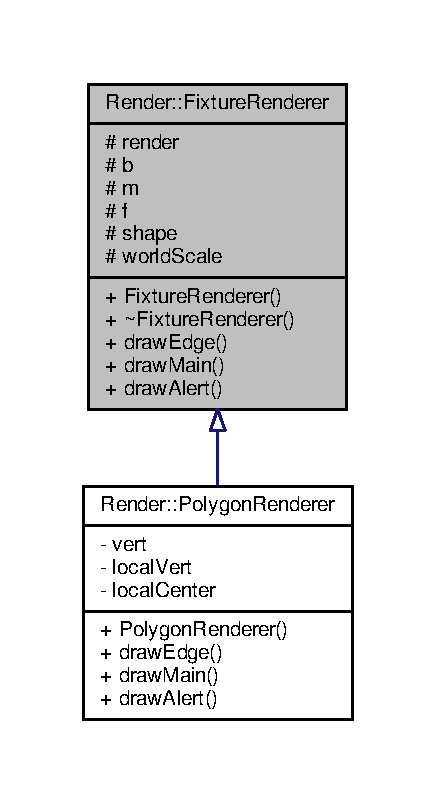
\includegraphics[width=209pt]{classRender_1_1FixtureRenderer__inherit__graph}
\end{center}
\end{figure}


Collaboration diagram for Render\+:\+:Fixture\+Renderer\+:
\nopagebreak
\begin{figure}[H]
\begin{center}
\leavevmode
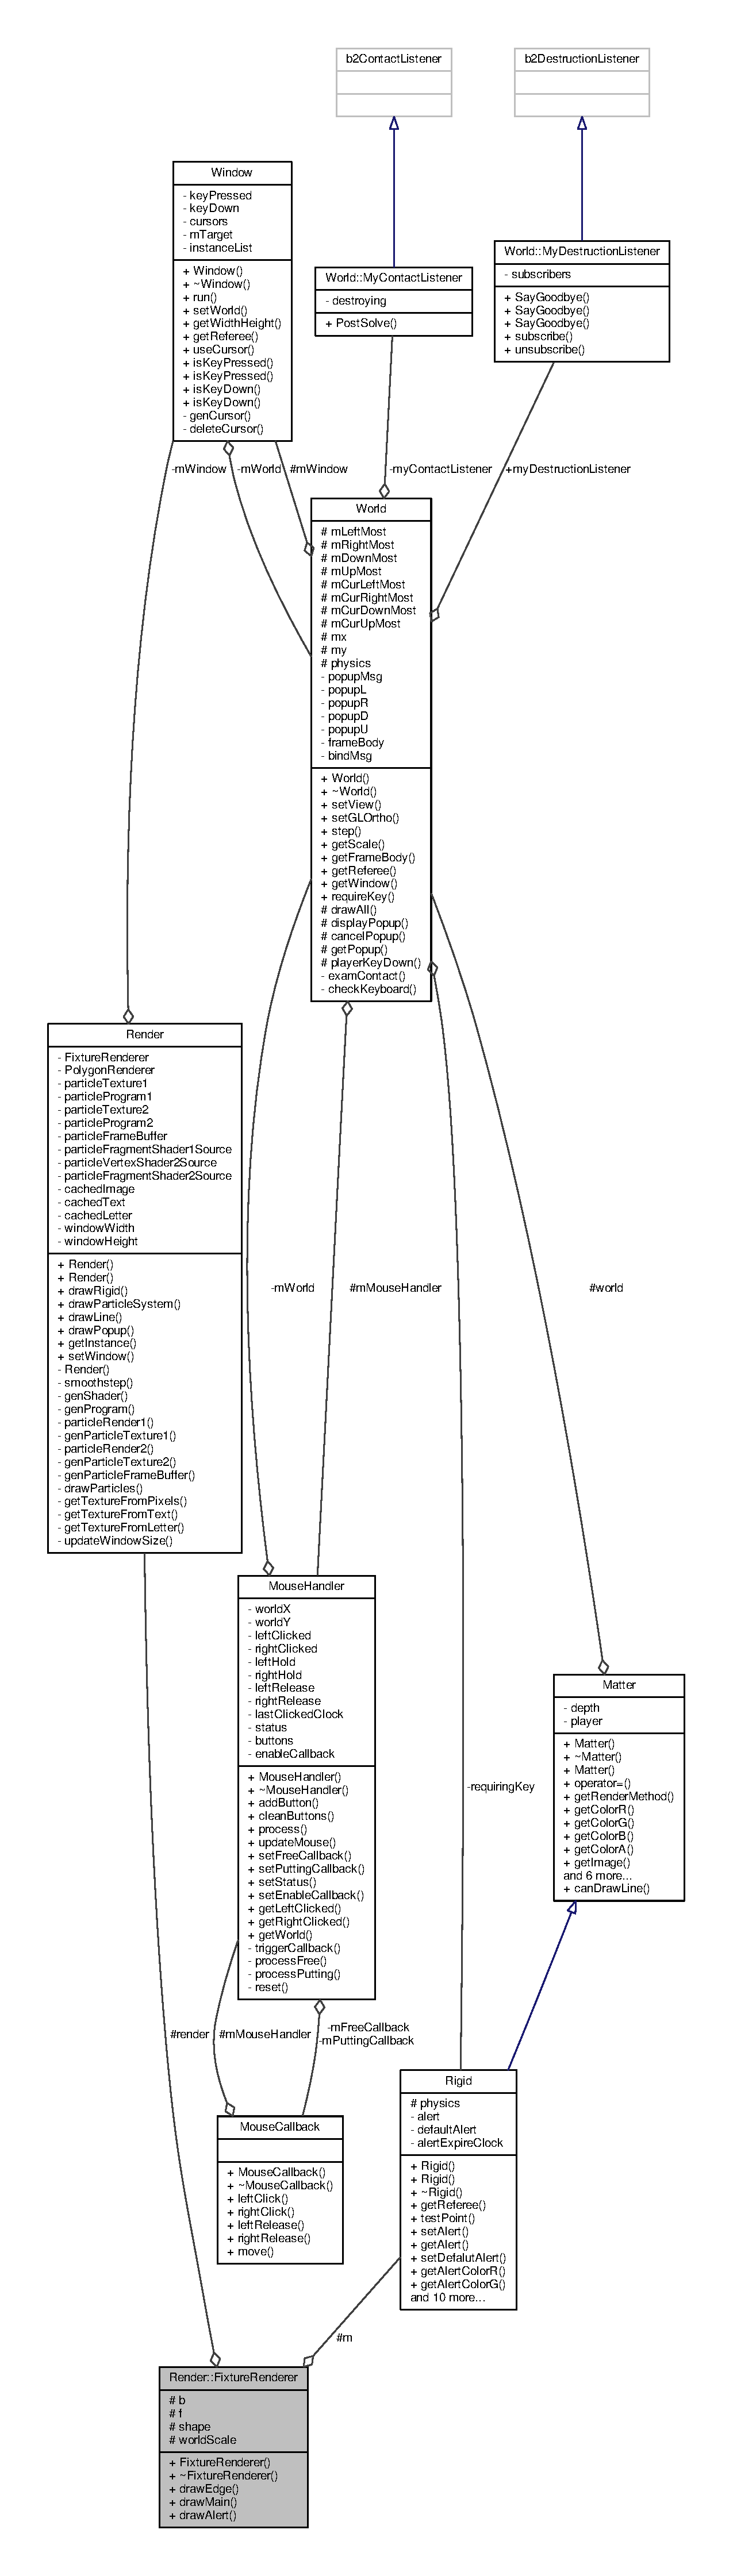
\includegraphics[height=550pt]{classRender_1_1FixtureRenderer__coll__graph}
\end{center}
\end{figure}
\subsection*{Public Member Functions}
\begin{DoxyCompactItemize}
\item 
\hyperlink{classRender_1_1FixtureRenderer_a5c2a71f6f1eabce19700ce57fb5a0c3b}{Fixture\+Renderer} (const b2\+Body $\ast$\+\_\+b, const b2\+Fixture $\ast$\+\_\+f, float \+\_\+scale) noexcept
\item 
virtual \hyperlink{classRender_1_1FixtureRenderer_a9c9dcfaa311b55a2e6f88eaa71c0f700}{$\sim$\+Fixture\+Renderer} () noexcept
\item 
virtual void \hyperlink{classRender_1_1FixtureRenderer_af0b5bfc5af5a2bb4a80eb7afc7e1398f}{draw\+Edge} () noexcept
\item 
virtual void \hyperlink{classRender_1_1FixtureRenderer_a20f23477aa8cc646f2d18b0165666e3b}{draw\+Main} () noexcept
\item 
virtual void \hyperlink{classRender_1_1FixtureRenderer_a3208fef7547ef2f61d68ddfd3ceb05da}{draw\+Alert} () noexcept
\end{DoxyCompactItemize}
\subsection*{Protected Attributes}
\begin{DoxyCompactItemize}
\item 
\hyperlink{classRender}{Render} \& \hyperlink{classRender_1_1FixtureRenderer_af093f28a7ea2cd706322636f5795098a}{render}
\item 
const b2\+Body $\ast$ \hyperlink{classRender_1_1FixtureRenderer_a61fdacb7120eef1444a8f4529a7dfe7c}{b}
\item 
const \hyperlink{classRigid}{Rigid} $\ast$ \hyperlink{classRender_1_1FixtureRenderer_af9c0ad74bd3b54e9112121221810fc9b}{m}
\item 
const b2\+Fixture $\ast$ \hyperlink{classRender_1_1FixtureRenderer_a85d6162146930c01082a48ae3d312fba}{f}
\item 
const b2\+Shape $\ast$ \hyperlink{classRender_1_1FixtureRenderer_a8332522b3b8a10f5f2772e5ca629cecb}{shape}
\item 
float \hyperlink{classRender_1_1FixtureRenderer_a0a11c59dbc0b65653c048e8900fdc12c}{world\+Scale}
\end{DoxyCompactItemize}


\subsection{Constructor \& Destructor Documentation}
\hypertarget{classRender_1_1FixtureRenderer_a5c2a71f6f1eabce19700ce57fb5a0c3b}{}\index{Render\+::\+Fixture\+Renderer@{Render\+::\+Fixture\+Renderer}!Fixture\+Renderer@{Fixture\+Renderer}}
\index{Fixture\+Renderer@{Fixture\+Renderer}!Render\+::\+Fixture\+Renderer@{Render\+::\+Fixture\+Renderer}}
\subsubsection[{Fixture\+Renderer}]{\setlength{\rightskip}{0pt plus 5cm}Render\+::\+Fixture\+Renderer\+::\+Fixture\+Renderer (
\begin{DoxyParamCaption}
\item[{const b2\+Body $\ast$}]{\+\_\+b, }
\item[{const b2\+Fixture $\ast$}]{\+\_\+f, }
\item[{float}]{\+\_\+scale}
\end{DoxyParamCaption}
)\hspace{0.3cm}{\ttfamily [noexcept]}}\label{classRender_1_1FixtureRenderer_a5c2a71f6f1eabce19700ce57fb5a0c3b}
\hypertarget{classRender_1_1FixtureRenderer_a9c9dcfaa311b55a2e6f88eaa71c0f700}{}\index{Render\+::\+Fixture\+Renderer@{Render\+::\+Fixture\+Renderer}!````~Fixture\+Renderer@{$\sim$\+Fixture\+Renderer}}
\index{````~Fixture\+Renderer@{$\sim$\+Fixture\+Renderer}!Render\+::\+Fixture\+Renderer@{Render\+::\+Fixture\+Renderer}}
\subsubsection[{$\sim$\+Fixture\+Renderer}]{\setlength{\rightskip}{0pt plus 5cm}virtual Render\+::\+Fixture\+Renderer\+::$\sim$\+Fixture\+Renderer (
\begin{DoxyParamCaption}
{}
\end{DoxyParamCaption}
)\hspace{0.3cm}{\ttfamily [inline]}, {\ttfamily [virtual]}, {\ttfamily [noexcept]}}\label{classRender_1_1FixtureRenderer_a9c9dcfaa311b55a2e6f88eaa71c0f700}


\subsection{Member Function Documentation}
\hypertarget{classRender_1_1FixtureRenderer_a3208fef7547ef2f61d68ddfd3ceb05da}{}\index{Render\+::\+Fixture\+Renderer@{Render\+::\+Fixture\+Renderer}!draw\+Alert@{draw\+Alert}}
\index{draw\+Alert@{draw\+Alert}!Render\+::\+Fixture\+Renderer@{Render\+::\+Fixture\+Renderer}}
\subsubsection[{draw\+Alert}]{\setlength{\rightskip}{0pt plus 5cm}virtual void Render\+::\+Fixture\+Renderer\+::draw\+Alert (
\begin{DoxyParamCaption}
{}
\end{DoxyParamCaption}
)\hspace{0.3cm}{\ttfamily [inline]}, {\ttfamily [virtual]}, {\ttfamily [noexcept]}}\label{classRender_1_1FixtureRenderer_a3208fef7547ef2f61d68ddfd3ceb05da}


Reimplemented in \hyperlink{classRender_1_1PolygonRenderer_ade951f9c8f1034823aecab89fe06aa9c}{Render\+::\+Polygon\+Renderer}.

\hypertarget{classRender_1_1FixtureRenderer_af0b5bfc5af5a2bb4a80eb7afc7e1398f}{}\index{Render\+::\+Fixture\+Renderer@{Render\+::\+Fixture\+Renderer}!draw\+Edge@{draw\+Edge}}
\index{draw\+Edge@{draw\+Edge}!Render\+::\+Fixture\+Renderer@{Render\+::\+Fixture\+Renderer}}
\subsubsection[{draw\+Edge}]{\setlength{\rightskip}{0pt plus 5cm}virtual void Render\+::\+Fixture\+Renderer\+::draw\+Edge (
\begin{DoxyParamCaption}
{}
\end{DoxyParamCaption}
)\hspace{0.3cm}{\ttfamily [inline]}, {\ttfamily [virtual]}, {\ttfamily [noexcept]}}\label{classRender_1_1FixtureRenderer_af0b5bfc5af5a2bb4a80eb7afc7e1398f}


Reimplemented in \hyperlink{classRender_1_1PolygonRenderer_af3e5d487898b3f7e0da7edcfc59967ba}{Render\+::\+Polygon\+Renderer}.

\hypertarget{classRender_1_1FixtureRenderer_a20f23477aa8cc646f2d18b0165666e3b}{}\index{Render\+::\+Fixture\+Renderer@{Render\+::\+Fixture\+Renderer}!draw\+Main@{draw\+Main}}
\index{draw\+Main@{draw\+Main}!Render\+::\+Fixture\+Renderer@{Render\+::\+Fixture\+Renderer}}
\subsubsection[{draw\+Main}]{\setlength{\rightskip}{0pt plus 5cm}virtual void Render\+::\+Fixture\+Renderer\+::draw\+Main (
\begin{DoxyParamCaption}
{}
\end{DoxyParamCaption}
)\hspace{0.3cm}{\ttfamily [inline]}, {\ttfamily [virtual]}, {\ttfamily [noexcept]}}\label{classRender_1_1FixtureRenderer_a20f23477aa8cc646f2d18b0165666e3b}


Reimplemented in \hyperlink{classRender_1_1PolygonRenderer_aec84603818d0ce8ba1805c4828505578}{Render\+::\+Polygon\+Renderer}.



\subsection{Member Data Documentation}
\hypertarget{classRender_1_1FixtureRenderer_a61fdacb7120eef1444a8f4529a7dfe7c}{}\index{Render\+::\+Fixture\+Renderer@{Render\+::\+Fixture\+Renderer}!b@{b}}
\index{b@{b}!Render\+::\+Fixture\+Renderer@{Render\+::\+Fixture\+Renderer}}
\subsubsection[{b}]{\setlength{\rightskip}{0pt plus 5cm}const b2\+Body$\ast$ Render\+::\+Fixture\+Renderer\+::b\hspace{0.3cm}{\ttfamily [protected]}}\label{classRender_1_1FixtureRenderer_a61fdacb7120eef1444a8f4529a7dfe7c}
\hypertarget{classRender_1_1FixtureRenderer_a85d6162146930c01082a48ae3d312fba}{}\index{Render\+::\+Fixture\+Renderer@{Render\+::\+Fixture\+Renderer}!f@{f}}
\index{f@{f}!Render\+::\+Fixture\+Renderer@{Render\+::\+Fixture\+Renderer}}
\subsubsection[{f}]{\setlength{\rightskip}{0pt plus 5cm}const b2\+Fixture$\ast$ Render\+::\+Fixture\+Renderer\+::f\hspace{0.3cm}{\ttfamily [protected]}}\label{classRender_1_1FixtureRenderer_a85d6162146930c01082a48ae3d312fba}
\hypertarget{classRender_1_1FixtureRenderer_af9c0ad74bd3b54e9112121221810fc9b}{}\index{Render\+::\+Fixture\+Renderer@{Render\+::\+Fixture\+Renderer}!m@{m}}
\index{m@{m}!Render\+::\+Fixture\+Renderer@{Render\+::\+Fixture\+Renderer}}
\subsubsection[{m}]{\setlength{\rightskip}{0pt plus 5cm}const {\bf Rigid}$\ast$ Render\+::\+Fixture\+Renderer\+::m\hspace{0.3cm}{\ttfamily [protected]}}\label{classRender_1_1FixtureRenderer_af9c0ad74bd3b54e9112121221810fc9b}
\hypertarget{classRender_1_1FixtureRenderer_af093f28a7ea2cd706322636f5795098a}{}\index{Render\+::\+Fixture\+Renderer@{Render\+::\+Fixture\+Renderer}!render@{render}}
\index{render@{render}!Render\+::\+Fixture\+Renderer@{Render\+::\+Fixture\+Renderer}}
\subsubsection[{render}]{\setlength{\rightskip}{0pt plus 5cm}{\bf Render}\& Render\+::\+Fixture\+Renderer\+::render\hspace{0.3cm}{\ttfamily [protected]}}\label{classRender_1_1FixtureRenderer_af093f28a7ea2cd706322636f5795098a}
\hypertarget{classRender_1_1FixtureRenderer_a8332522b3b8a10f5f2772e5ca629cecb}{}\index{Render\+::\+Fixture\+Renderer@{Render\+::\+Fixture\+Renderer}!shape@{shape}}
\index{shape@{shape}!Render\+::\+Fixture\+Renderer@{Render\+::\+Fixture\+Renderer}}
\subsubsection[{shape}]{\setlength{\rightskip}{0pt plus 5cm}const b2\+Shape$\ast$ Render\+::\+Fixture\+Renderer\+::shape\hspace{0.3cm}{\ttfamily [protected]}}\label{classRender_1_1FixtureRenderer_a8332522b3b8a10f5f2772e5ca629cecb}
\hypertarget{classRender_1_1FixtureRenderer_a0a11c59dbc0b65653c048e8900fdc12c}{}\index{Render\+::\+Fixture\+Renderer@{Render\+::\+Fixture\+Renderer}!world\+Scale@{world\+Scale}}
\index{world\+Scale@{world\+Scale}!Render\+::\+Fixture\+Renderer@{Render\+::\+Fixture\+Renderer}}
\subsubsection[{world\+Scale}]{\setlength{\rightskip}{0pt plus 5cm}float Render\+::\+Fixture\+Renderer\+::world\+Scale\hspace{0.3cm}{\ttfamily [protected]}}\label{classRender_1_1FixtureRenderer_a0a11c59dbc0b65653c048e8900fdc12c}


The documentation for this class was generated from the following files\+:\begin{DoxyCompactItemize}
\item 
\hyperlink{render_8h}{render.\+h}\item 
\hyperlink{render_8cpp}{render.\+cpp}\end{DoxyCompactItemize}

\hypertarget{classFlame}{}\section{Flame Class Reference}
\label{classFlame}\index{Flame@{Flame}}


Set when bomb exploses.  




{\ttfamily \#include $<$matter.\+h$>$}



Inheritance diagram for Flame\+:\nopagebreak
\begin{figure}[H]
\begin{center}
\leavevmode
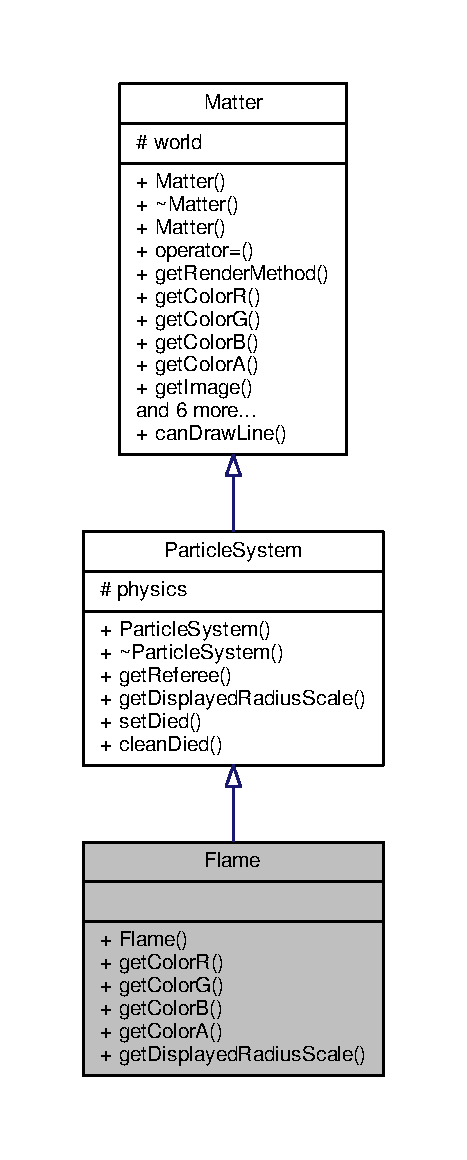
\includegraphics[height=550pt]{classFlame__inherit__graph}
\end{center}
\end{figure}


Collaboration diagram for Flame\+:\nopagebreak
\begin{figure}[H]
\begin{center}
\leavevmode
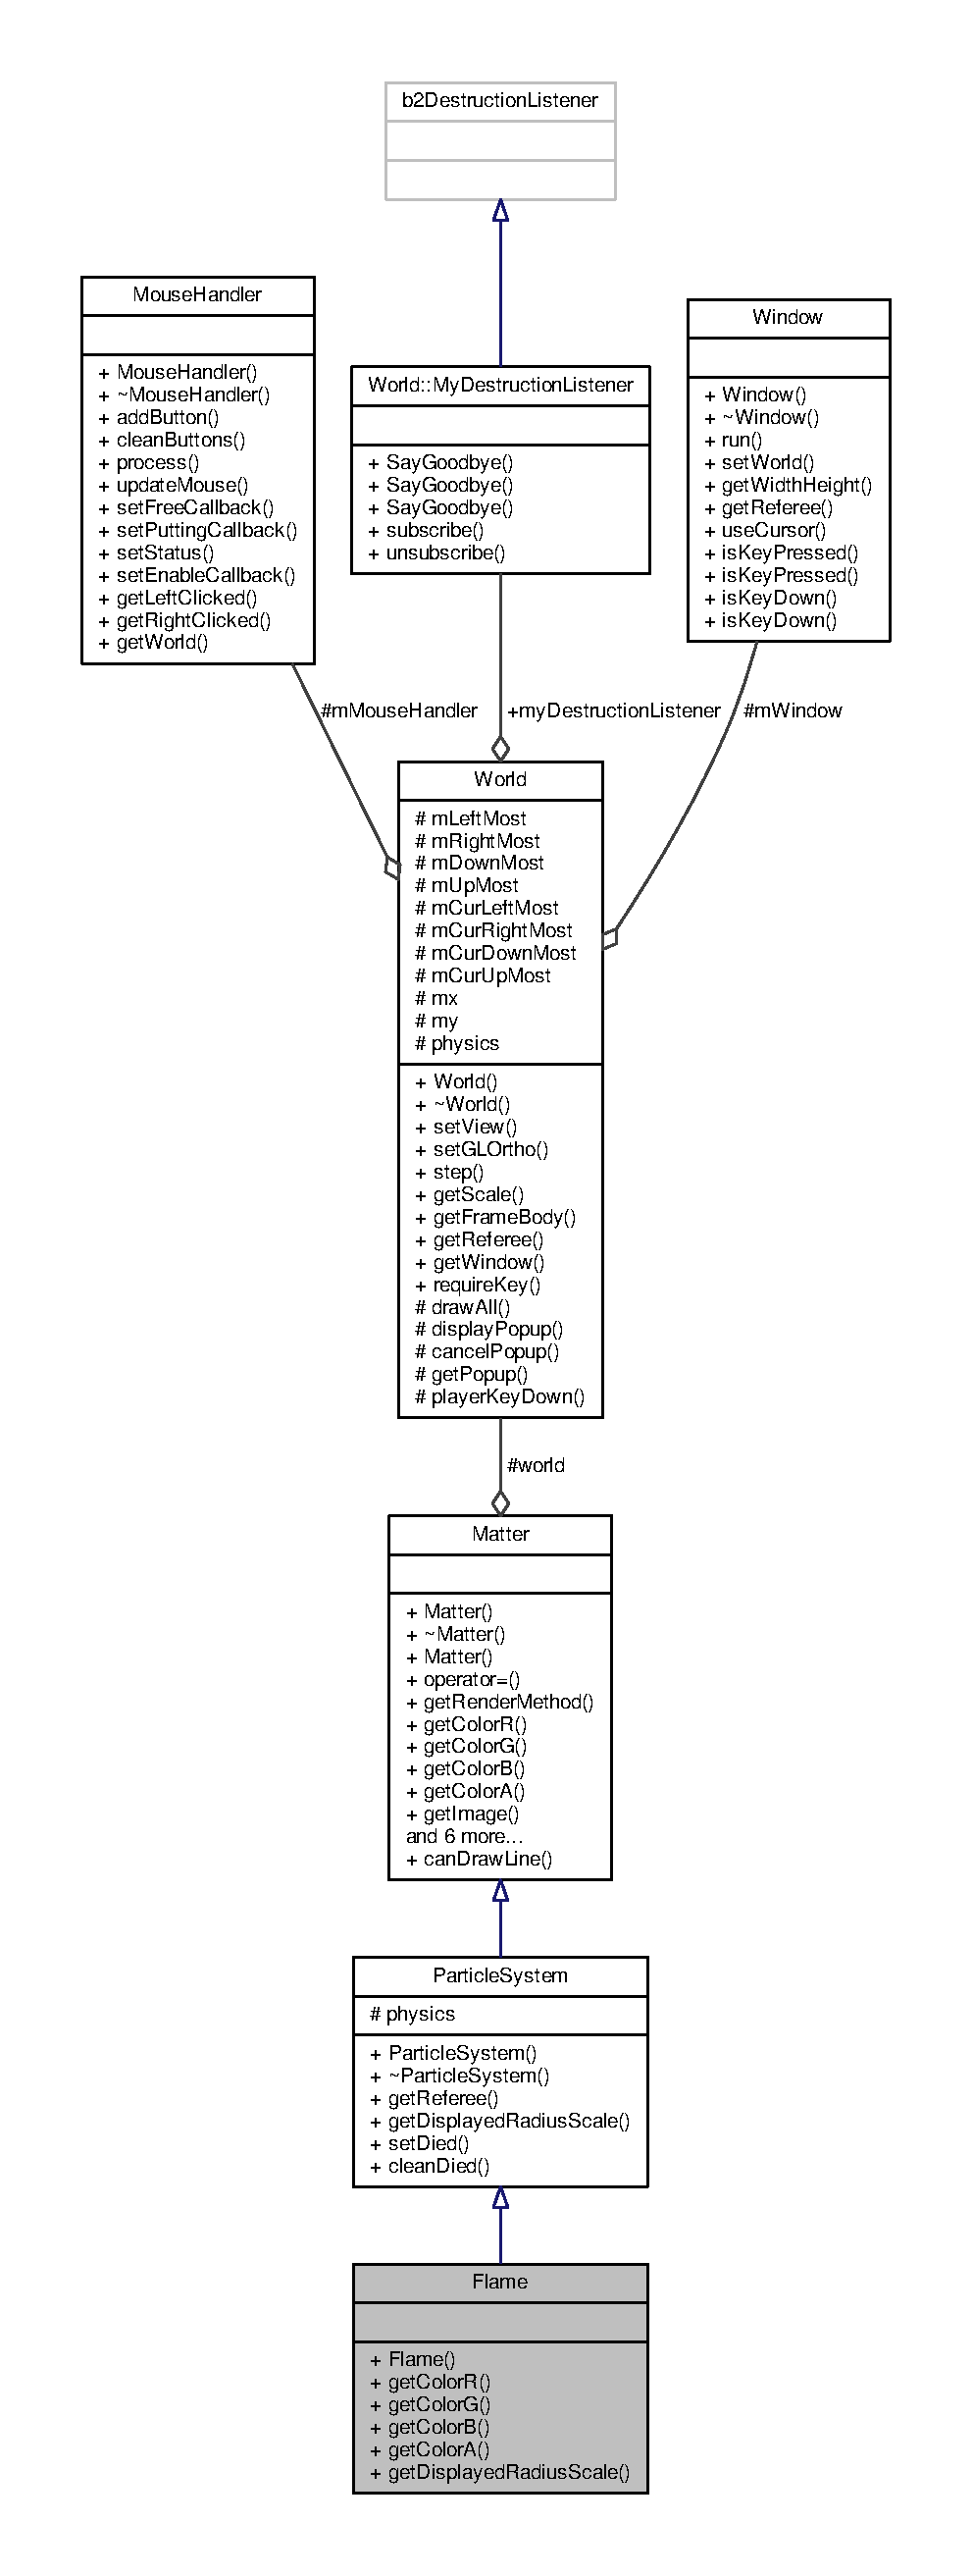
\includegraphics[height=550pt]{classFlame__coll__graph}
\end{center}
\end{figure}
\subsection*{Public Member Functions}
\begin{DoxyCompactItemize}
\item 
\hyperlink{classFlame_af76751e5a5bc652873134f5f21995ea1}{Flame} (\hyperlink{classWorld}{World} $\ast$\+\_\+world, const b2\+Vec2 \&pos, float radius) noexcept
\item 
virtual float \hyperlink{classFlame_a3cdb607d9cadaeb164494ea2334c4bf8}{get\+Color\+R} () const override
\item 
virtual float \hyperlink{classFlame_a52151a48e25d77440ea47b3479501d36}{get\+Color\+G} () const override
\item 
virtual float \hyperlink{classFlame_abbd9b48e0a3744f4a9c59df52e8c8ca1}{get\+Color\+B} () const override
\item 
virtual float \hyperlink{classFlame_a9730bb5ff22bdf2ab579eb9ae1d8a37f}{get\+Color\+A} () const override
\item 
virtual float \hyperlink{classFlame_a472dc6269e6e13b4628abd2392726fd8}{get\+Displayed\+Radius\+Scale} () const override
\begin{DoxyCompactList}\small\item\em displayed radius = ? $\ast$ physics radius \end{DoxyCompactList}\end{DoxyCompactItemize}
\subsection*{Additional Inherited Members}


\subsection{Detailed Description}
Set when bomb exploses. 

\subsection{Constructor \& Destructor Documentation}
\hypertarget{classFlame_af76751e5a5bc652873134f5f21995ea1}{}\index{Flame@{Flame}!Flame@{Flame}}
\index{Flame@{Flame}!Flame@{Flame}}
\subsubsection[{Flame}]{\setlength{\rightskip}{0pt plus 5cm}Flame\+::\+Flame (
\begin{DoxyParamCaption}
\item[{{\bf World} $\ast$}]{\+\_\+world, }
\item[{const b2\+Vec2 \&}]{pos, }
\item[{float}]{radius}
\end{DoxyParamCaption}
)\hspace{0.3cm}{\ttfamily [noexcept]}}\label{classFlame_af76751e5a5bc652873134f5f21995ea1}


\subsection{Member Function Documentation}
\hypertarget{classFlame_a9730bb5ff22bdf2ab579eb9ae1d8a37f}{}\index{Flame@{Flame}!get\+Color\+A@{get\+Color\+A}}
\index{get\+Color\+A@{get\+Color\+A}!Flame@{Flame}}
\subsubsection[{get\+Color\+A}]{\setlength{\rightskip}{0pt plus 5cm}virtual float Flame\+::get\+Color\+A (
\begin{DoxyParamCaption}
{}
\end{DoxyParamCaption}
) const\hspace{0.3cm}{\ttfamily [inline]}, {\ttfamily [override]}, {\ttfamily [virtual]}}\label{classFlame_a9730bb5ff22bdf2ab579eb9ae1d8a37f}


Reimplemented from \hyperlink{classMatter_aa44ee7ba48cb9a582a6f86e1e9e2ef38}{Matter}.

\hypertarget{classFlame_abbd9b48e0a3744f4a9c59df52e8c8ca1}{}\index{Flame@{Flame}!get\+Color\+B@{get\+Color\+B}}
\index{get\+Color\+B@{get\+Color\+B}!Flame@{Flame}}
\subsubsection[{get\+Color\+B}]{\setlength{\rightskip}{0pt plus 5cm}virtual float Flame\+::get\+Color\+B (
\begin{DoxyParamCaption}
{}
\end{DoxyParamCaption}
) const\hspace{0.3cm}{\ttfamily [inline]}, {\ttfamily [override]}, {\ttfamily [virtual]}}\label{classFlame_abbd9b48e0a3744f4a9c59df52e8c8ca1}


Reimplemented from \hyperlink{classMatter_af830da17da427c84c7f6deee4a91b3d4}{Matter}.

\hypertarget{classFlame_a52151a48e25d77440ea47b3479501d36}{}\index{Flame@{Flame}!get\+Color\+G@{get\+Color\+G}}
\index{get\+Color\+G@{get\+Color\+G}!Flame@{Flame}}
\subsubsection[{get\+Color\+G}]{\setlength{\rightskip}{0pt plus 5cm}virtual float Flame\+::get\+Color\+G (
\begin{DoxyParamCaption}
{}
\end{DoxyParamCaption}
) const\hspace{0.3cm}{\ttfamily [inline]}, {\ttfamily [override]}, {\ttfamily [virtual]}}\label{classFlame_a52151a48e25d77440ea47b3479501d36}


Reimplemented from \hyperlink{classMatter_aa3fcdc82f788fbf873ec3ff4808f614a}{Matter}.

\hypertarget{classFlame_a3cdb607d9cadaeb164494ea2334c4bf8}{}\index{Flame@{Flame}!get\+Color\+R@{get\+Color\+R}}
\index{get\+Color\+R@{get\+Color\+R}!Flame@{Flame}}
\subsubsection[{get\+Color\+R}]{\setlength{\rightskip}{0pt plus 5cm}virtual float Flame\+::get\+Color\+R (
\begin{DoxyParamCaption}
{}
\end{DoxyParamCaption}
) const\hspace{0.3cm}{\ttfamily [inline]}, {\ttfamily [override]}, {\ttfamily [virtual]}}\label{classFlame_a3cdb607d9cadaeb164494ea2334c4bf8}


Reimplemented from \hyperlink{classMatter_a926d246584228c3e3b102dbfd42036ec}{Matter}.

\hypertarget{classFlame_a472dc6269e6e13b4628abd2392726fd8}{}\index{Flame@{Flame}!get\+Displayed\+Radius\+Scale@{get\+Displayed\+Radius\+Scale}}
\index{get\+Displayed\+Radius\+Scale@{get\+Displayed\+Radius\+Scale}!Flame@{Flame}}
\subsubsection[{get\+Displayed\+Radius\+Scale}]{\setlength{\rightskip}{0pt plus 5cm}virtual float Flame\+::get\+Displayed\+Radius\+Scale (
\begin{DoxyParamCaption}
{}
\end{DoxyParamCaption}
) const\hspace{0.3cm}{\ttfamily [inline]}, {\ttfamily [override]}, {\ttfamily [virtual]}}\label{classFlame_a472dc6269e6e13b4628abd2392726fd8}


displayed radius = ? $\ast$ physics radius 



Implements \hyperlink{classParticleSystem_a5b3bcfbc82de5d335f55173b049da517}{Particle\+System}.



The documentation for this class was generated from the following files\+:\begin{DoxyCompactItemize}
\item 
\hyperlink{matter_8h}{matter.\+h}\item 
\hyperlink{matter_8cpp}{matter.\+cpp}\end{DoxyCompactItemize}

\hypertarget{classFrame}{}\section{Frame Class Reference}
\label{classFrame}\index{Frame@{Frame}}


\hyperlink{classFrame}{Frame} around the world 1 unit thick.  




{\ttfamily \#include $<$matter.\+h$>$}



Inheritance diagram for Frame\+:\nopagebreak
\begin{figure}[H]
\begin{center}
\leavevmode
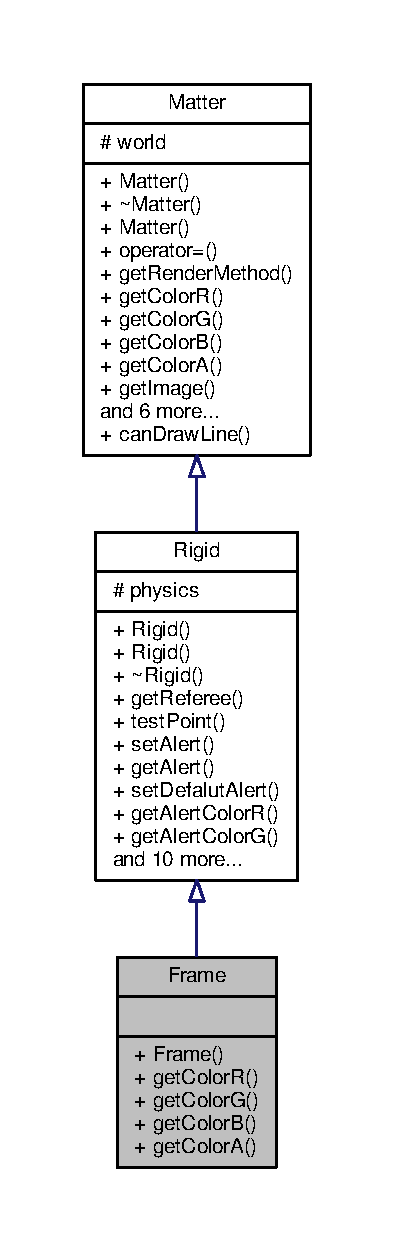
\includegraphics[height=550pt]{classFrame__inherit__graph}
\end{center}
\end{figure}


Collaboration diagram for Frame\+:\nopagebreak
\begin{figure}[H]
\begin{center}
\leavevmode
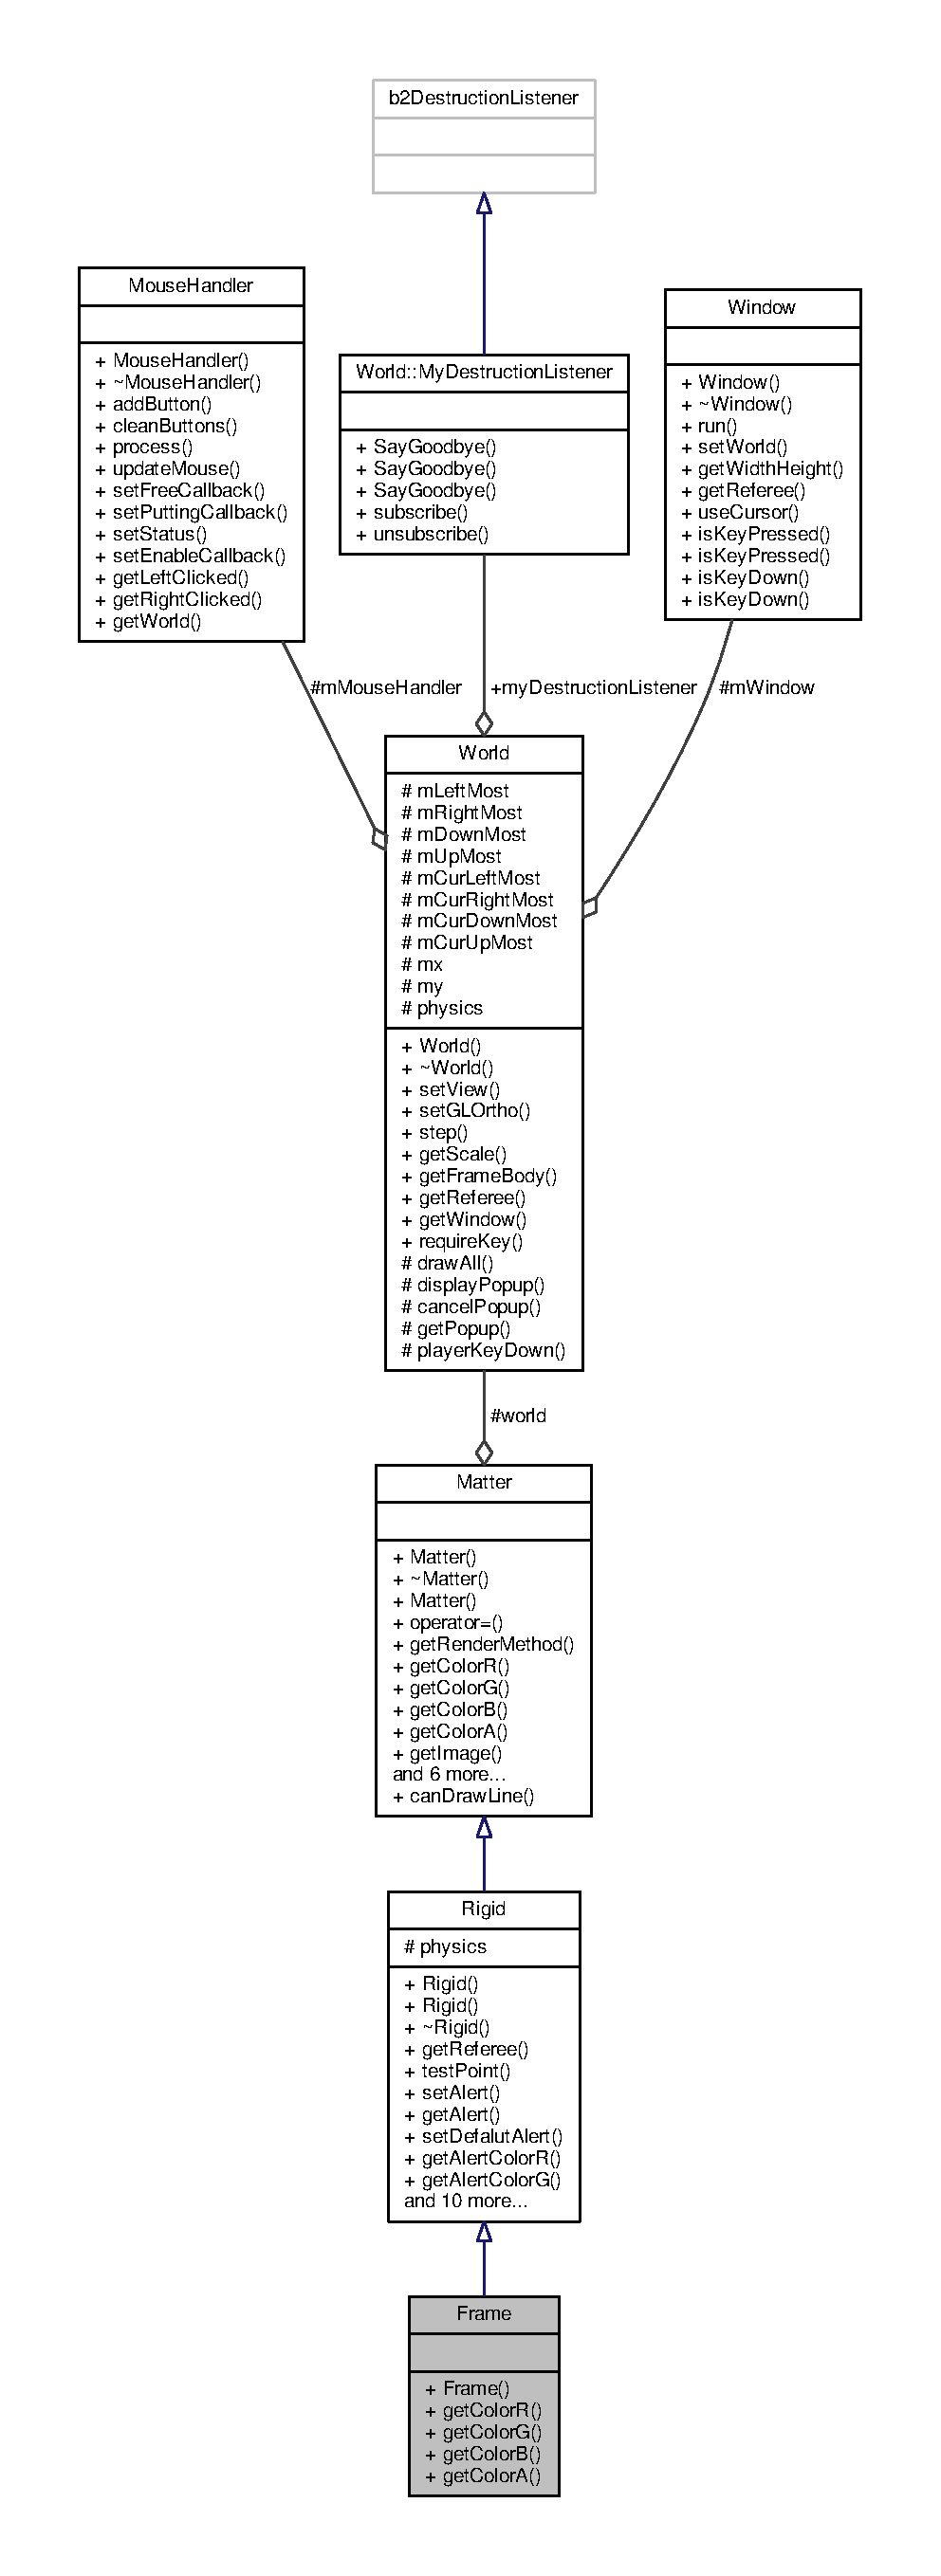
\includegraphics[height=550pt]{classFrame__coll__graph}
\end{center}
\end{figure}
\subsection*{Public Member Functions}
\begin{DoxyCompactItemize}
\item 
\hyperlink{classFrame_acfe3dc2087b63497a740317623e4d7ff}{Frame} (\hyperlink{classWorld}{World} $\ast$\+\_\+world, float l, float \hyperlink{image_8h_a62969232668331297e2dca1ae2ddd10d}{r}, float d, float u) noexcept
\item 
virtual float \hyperlink{classFrame_a1f5aa3b4dd7b90959a95c1e54f01a1e4}{get\+Color\+R} () const 
\item 
virtual float \hyperlink{classFrame_a44139c9e8bee6504c43bb6bc21b1d599}{get\+Color\+G} () const 
\item 
virtual float \hyperlink{classFrame_aac730f8f9ae5f59cb6a1814d56a8eefa}{get\+Color\+B} () const 
\item 
virtual float \hyperlink{classFrame_a99769eacd74a31fc9d198f83bc6616db}{get\+Color\+A} () const 
\end{DoxyCompactItemize}
\subsection*{Additional Inherited Members}


\subsection{Detailed Description}
\hyperlink{classFrame}{Frame} around the world 1 unit thick. 

\subsection{Constructor \& Destructor Documentation}
\hypertarget{classFrame_acfe3dc2087b63497a740317623e4d7ff}{}\index{Frame@{Frame}!Frame@{Frame}}
\index{Frame@{Frame}!Frame@{Frame}}
\subsubsection[{Frame}]{\setlength{\rightskip}{0pt plus 5cm}Frame\+::\+Frame (
\begin{DoxyParamCaption}
\item[{{\bf World} $\ast$}]{\+\_\+world, }
\item[{float}]{l, }
\item[{float}]{r, }
\item[{float}]{d, }
\item[{float}]{u}
\end{DoxyParamCaption}
)\hspace{0.3cm}{\ttfamily [noexcept]}}\label{classFrame_acfe3dc2087b63497a740317623e4d7ff}


\subsection{Member Function Documentation}
\hypertarget{classFrame_a99769eacd74a31fc9d198f83bc6616db}{}\index{Frame@{Frame}!get\+Color\+A@{get\+Color\+A}}
\index{get\+Color\+A@{get\+Color\+A}!Frame@{Frame}}
\subsubsection[{get\+Color\+A}]{\setlength{\rightskip}{0pt plus 5cm}virtual float Frame\+::get\+Color\+A (
\begin{DoxyParamCaption}
{}
\end{DoxyParamCaption}
) const\hspace{0.3cm}{\ttfamily [inline]}, {\ttfamily [virtual]}}\label{classFrame_a99769eacd74a31fc9d198f83bc6616db}


Reimplemented from \hyperlink{classMatter_aa44ee7ba48cb9a582a6f86e1e9e2ef38}{Matter}.

\hypertarget{classFrame_aac730f8f9ae5f59cb6a1814d56a8eefa}{}\index{Frame@{Frame}!get\+Color\+B@{get\+Color\+B}}
\index{get\+Color\+B@{get\+Color\+B}!Frame@{Frame}}
\subsubsection[{get\+Color\+B}]{\setlength{\rightskip}{0pt plus 5cm}virtual float Frame\+::get\+Color\+B (
\begin{DoxyParamCaption}
{}
\end{DoxyParamCaption}
) const\hspace{0.3cm}{\ttfamily [inline]}, {\ttfamily [virtual]}}\label{classFrame_aac730f8f9ae5f59cb6a1814d56a8eefa}


Reimplemented from \hyperlink{classMatter_af830da17da427c84c7f6deee4a91b3d4}{Matter}.

\hypertarget{classFrame_a44139c9e8bee6504c43bb6bc21b1d599}{}\index{Frame@{Frame}!get\+Color\+G@{get\+Color\+G}}
\index{get\+Color\+G@{get\+Color\+G}!Frame@{Frame}}
\subsubsection[{get\+Color\+G}]{\setlength{\rightskip}{0pt plus 5cm}virtual float Frame\+::get\+Color\+G (
\begin{DoxyParamCaption}
{}
\end{DoxyParamCaption}
) const\hspace{0.3cm}{\ttfamily [inline]}, {\ttfamily [virtual]}}\label{classFrame_a44139c9e8bee6504c43bb6bc21b1d599}


Reimplemented from \hyperlink{classMatter_aa3fcdc82f788fbf873ec3ff4808f614a}{Matter}.

\hypertarget{classFrame_a1f5aa3b4dd7b90959a95c1e54f01a1e4}{}\index{Frame@{Frame}!get\+Color\+R@{get\+Color\+R}}
\index{get\+Color\+R@{get\+Color\+R}!Frame@{Frame}}
\subsubsection[{get\+Color\+R}]{\setlength{\rightskip}{0pt plus 5cm}virtual float Frame\+::get\+Color\+R (
\begin{DoxyParamCaption}
{}
\end{DoxyParamCaption}
) const\hspace{0.3cm}{\ttfamily [inline]}, {\ttfamily [virtual]}}\label{classFrame_a1f5aa3b4dd7b90959a95c1e54f01a1e4}


Reimplemented from \hyperlink{classMatter_a926d246584228c3e3b102dbfd42036ec}{Matter}.



The documentation for this class was generated from the following files\+:\begin{DoxyCompactItemize}
\item 
\hyperlink{matter_8h}{matter.\+h}\item 
\hyperlink{matter_8cpp}{matter.\+cpp}\end{DoxyCompactItemize}

\hypertarget{classWorld_1_1GlobalTestPoint}{}\section{World\+:\+:Global\+Test\+Point Class Reference}
\label{classWorld_1_1GlobalTestPoint}\index{World\+::\+Global\+Test\+Point@{World\+::\+Global\+Test\+Point}}


A helper for finding a fixture overlapping with a point.  




{\ttfamily \#include $<$world.\+h$>$}



Inheritance diagram for World\+:\+:Global\+Test\+Point\+:
\nopagebreak
\begin{figure}[H]
\begin{center}
\leavevmode
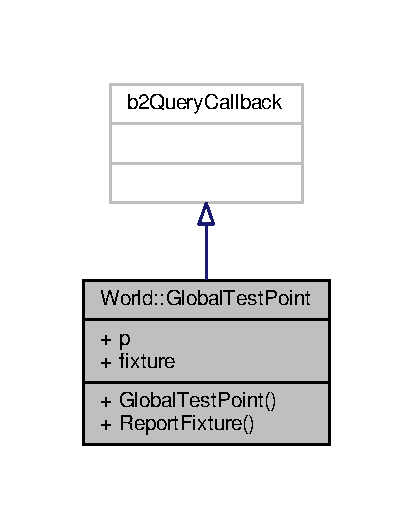
\includegraphics[width=198pt]{classWorld_1_1GlobalTestPoint__inherit__graph}
\end{center}
\end{figure}


Collaboration diagram for World\+:\+:Global\+Test\+Point\+:
\nopagebreak
\begin{figure}[H]
\begin{center}
\leavevmode
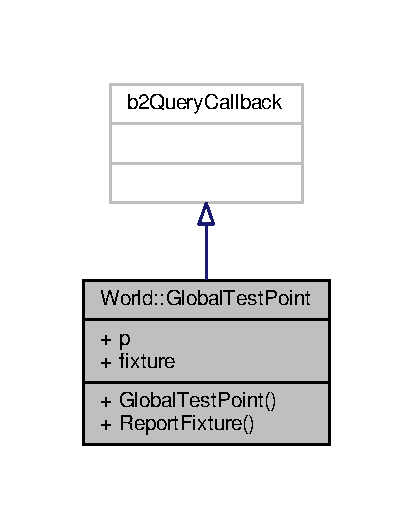
\includegraphics[width=198pt]{classWorld_1_1GlobalTestPoint__coll__graph}
\end{center}
\end{figure}
\subsection*{Public Member Functions}
\begin{DoxyCompactItemize}
\item 
\hyperlink{classWorld_1_1GlobalTestPoint_ab2c8dd2b120a990c45bf550229d43660}{Global\+Test\+Point} (const b2\+Vec2 \&\+\_\+p)
\item 
bool \hyperlink{classWorld_1_1GlobalTestPoint_a795e9a32de4d2d49f8d522c3a8cefa6a}{Report\+Fixture} (b2\+Fixture $\ast$\+\_\+f) override
\end{DoxyCompactItemize}
\subsection*{Public Attributes}
\begin{DoxyCompactItemize}
\item 
b2\+Vec2 \hyperlink{classWorld_1_1GlobalTestPoint_a319e7d54c671520383e9bc9e11c261d4}{p}
\item 
b2\+Fixture $\ast$ \hyperlink{classWorld_1_1GlobalTestPoint_a15844bf58ea05cde3abfae303f58d137}{fixture}
\end{DoxyCompactItemize}


\subsection{Detailed Description}
A helper for finding a fixture overlapping with a point. 

\subsection{Constructor \& Destructor Documentation}
\hypertarget{classWorld_1_1GlobalTestPoint_ab2c8dd2b120a990c45bf550229d43660}{}\index{World\+::\+Global\+Test\+Point@{World\+::\+Global\+Test\+Point}!Global\+Test\+Point@{Global\+Test\+Point}}
\index{Global\+Test\+Point@{Global\+Test\+Point}!World\+::\+Global\+Test\+Point@{World\+::\+Global\+Test\+Point}}
\subsubsection[{Global\+Test\+Point}]{\setlength{\rightskip}{0pt plus 5cm}World\+::\+Global\+Test\+Point\+::\+Global\+Test\+Point (
\begin{DoxyParamCaption}
\item[{const b2\+Vec2 \&}]{\+\_\+p}
\end{DoxyParamCaption}
)\hspace{0.3cm}{\ttfamily [inline]}}\label{classWorld_1_1GlobalTestPoint_ab2c8dd2b120a990c45bf550229d43660}


\subsection{Member Function Documentation}
\hypertarget{classWorld_1_1GlobalTestPoint_a795e9a32de4d2d49f8d522c3a8cefa6a}{}\index{World\+::\+Global\+Test\+Point@{World\+::\+Global\+Test\+Point}!Report\+Fixture@{Report\+Fixture}}
\index{Report\+Fixture@{Report\+Fixture}!World\+::\+Global\+Test\+Point@{World\+::\+Global\+Test\+Point}}
\subsubsection[{Report\+Fixture}]{\setlength{\rightskip}{0pt plus 5cm}bool World\+::\+Global\+Test\+Point\+::\+Report\+Fixture (
\begin{DoxyParamCaption}
\item[{b2\+Fixture $\ast$}]{\+\_\+f}
\end{DoxyParamCaption}
)\hspace{0.3cm}{\ttfamily [override]}}\label{classWorld_1_1GlobalTestPoint_a795e9a32de4d2d49f8d522c3a8cefa6a}


\subsection{Member Data Documentation}
\hypertarget{classWorld_1_1GlobalTestPoint_a15844bf58ea05cde3abfae303f58d137}{}\index{World\+::\+Global\+Test\+Point@{World\+::\+Global\+Test\+Point}!fixture@{fixture}}
\index{fixture@{fixture}!World\+::\+Global\+Test\+Point@{World\+::\+Global\+Test\+Point}}
\subsubsection[{fixture}]{\setlength{\rightskip}{0pt plus 5cm}b2\+Fixture$\ast$ World\+::\+Global\+Test\+Point\+::fixture}\label{classWorld_1_1GlobalTestPoint_a15844bf58ea05cde3abfae303f58d137}
\hypertarget{classWorld_1_1GlobalTestPoint_a319e7d54c671520383e9bc9e11c261d4}{}\index{World\+::\+Global\+Test\+Point@{World\+::\+Global\+Test\+Point}!p@{p}}
\index{p@{p}!World\+::\+Global\+Test\+Point@{World\+::\+Global\+Test\+Point}}
\subsubsection[{p}]{\setlength{\rightskip}{0pt plus 5cm}b2\+Vec2 World\+::\+Global\+Test\+Point\+::p}\label{classWorld_1_1GlobalTestPoint_a319e7d54c671520383e9bc9e11c261d4}


The documentation for this class was generated from the following files\+:\begin{DoxyCompactItemize}
\item 
\hyperlink{world_8h}{world.\+h}\item 
\hyperlink{world_8cpp}{world.\+cpp}\end{DoxyCompactItemize}

\hypertarget{classLargeEngine}{}\section{Large\+Engine Class Reference}
\label{classLargeEngine}\index{Large\+Engine@{Large\+Engine}}


2\+X4 Large engine that will provide a 300\+N force  




{\ttfamily \#include $<$matter.\+h$>$}



Inheritance diagram for Large\+Engine\+:
\nopagebreak
\begin{figure}[H]
\begin{center}
\leavevmode
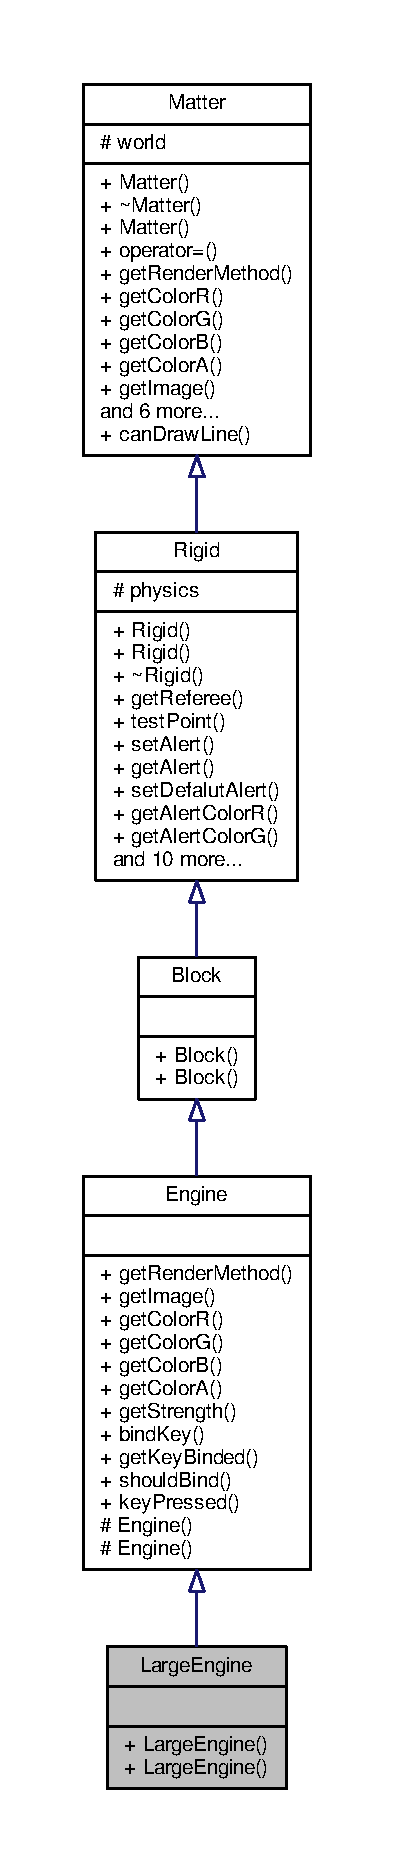
\includegraphics[height=550pt]{classLargeEngine__inherit__graph}
\end{center}
\end{figure}


Collaboration diagram for Large\+Engine\+:
\nopagebreak
\begin{figure}[H]
\begin{center}
\leavevmode
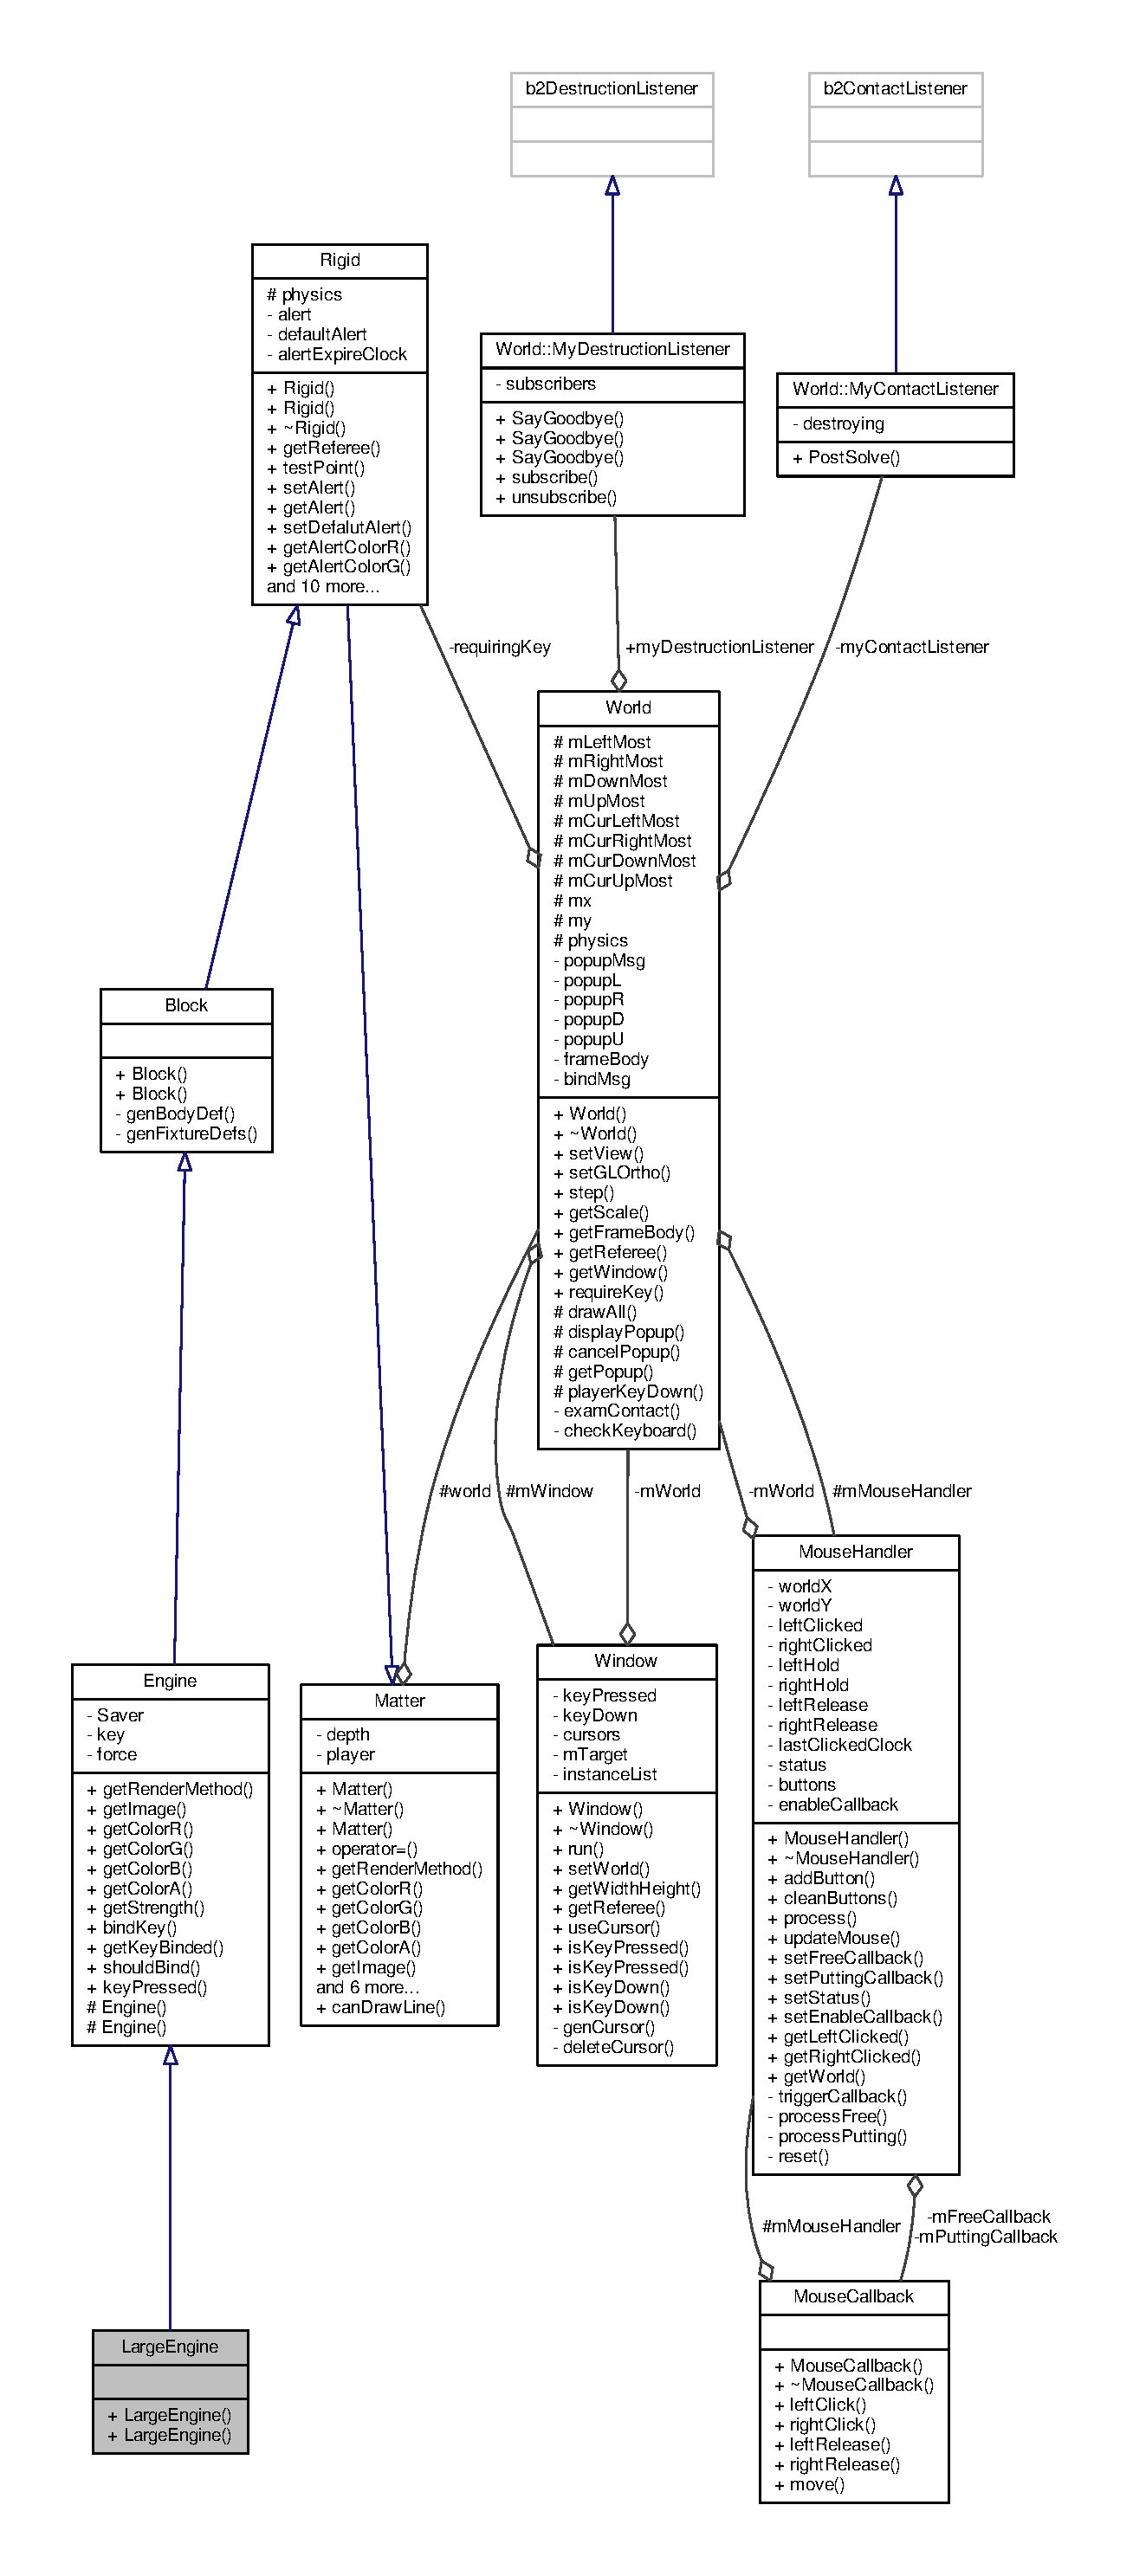
\includegraphics[height=550pt]{classLargeEngine__coll__graph}
\end{center}
\end{figure}
\subsection*{Public Member Functions}
\begin{DoxyCompactItemize}
\item 
\hyperlink{classLargeEngine_a756c59d574466007d596649bd3fe5504}{Large\+Engine} (\hyperlink{classWorld}{World} $\ast$\+\_\+world, b2\+Body $\ast$\hyperlink{image_8h_ab2d05693952610f937e5acb3c4a8fa1b}{b})
\item 
\hyperlink{classLargeEngine_a02b3d03941f0d1a554f0ce7e22938fd6}{Large\+Engine} (\hyperlink{classWorld}{World} $\ast$\+\_\+world, float x, float y, float notused1=0, float notused2=0) noexcept
\end{DoxyCompactItemize}
\subsection*{Additional Inherited Members}


\subsection{Detailed Description}
2\+X4 Large engine that will provide a 300\+N force 

\subsection{Constructor \& Destructor Documentation}
\hypertarget{classLargeEngine_a756c59d574466007d596649bd3fe5504}{}\index{Large\+Engine@{Large\+Engine}!Large\+Engine@{Large\+Engine}}
\index{Large\+Engine@{Large\+Engine}!Large\+Engine@{Large\+Engine}}
\subsubsection[{Large\+Engine}]{\setlength{\rightskip}{0pt plus 5cm}Large\+Engine\+::\+Large\+Engine (
\begin{DoxyParamCaption}
\item[{{\bf World} $\ast$}]{\+\_\+world, }
\item[{b2\+Body $\ast$}]{b}
\end{DoxyParamCaption}
)\hspace{0.3cm}{\ttfamily [inline]}}\label{classLargeEngine_a756c59d574466007d596649bd3fe5504}
\hypertarget{classLargeEngine_a02b3d03941f0d1a554f0ce7e22938fd6}{}\index{Large\+Engine@{Large\+Engine}!Large\+Engine@{Large\+Engine}}
\index{Large\+Engine@{Large\+Engine}!Large\+Engine@{Large\+Engine}}
\subsubsection[{Large\+Engine}]{\setlength{\rightskip}{0pt plus 5cm}Large\+Engine\+::\+Large\+Engine (
\begin{DoxyParamCaption}
\item[{{\bf World} $\ast$}]{\+\_\+world, }
\item[{float}]{x, }
\item[{float}]{y, }
\item[{float}]{notused1 = {\ttfamily 0}, }
\item[{float}]{notused2 = {\ttfamily 0}}
\end{DoxyParamCaption}
)\hspace{0.3cm}{\ttfamily [inline]}, {\ttfamily [noexcept]}}\label{classLargeEngine_a02b3d03941f0d1a554f0ce7e22938fd6}


The documentation for this class was generated from the following file\+:\begin{DoxyCompactItemize}
\item 
\hyperlink{matter_8h}{matter.\+h}\end{DoxyCompactItemize}

\hypertarget{classLargeWoodBlock}{}\section{Large\+Wood\+Block Class Reference}
\label{classLargeWoodBlock}\index{Large\+Wood\+Block@{Large\+Wood\+Block}}


Dynamic 3\+X3 large wooden block Will Float.  




{\ttfamily \#include $<$matter.\+h$>$}



Inheritance diagram for Large\+Wood\+Block\+:\nopagebreak
\begin{figure}[H]
\begin{center}
\leavevmode
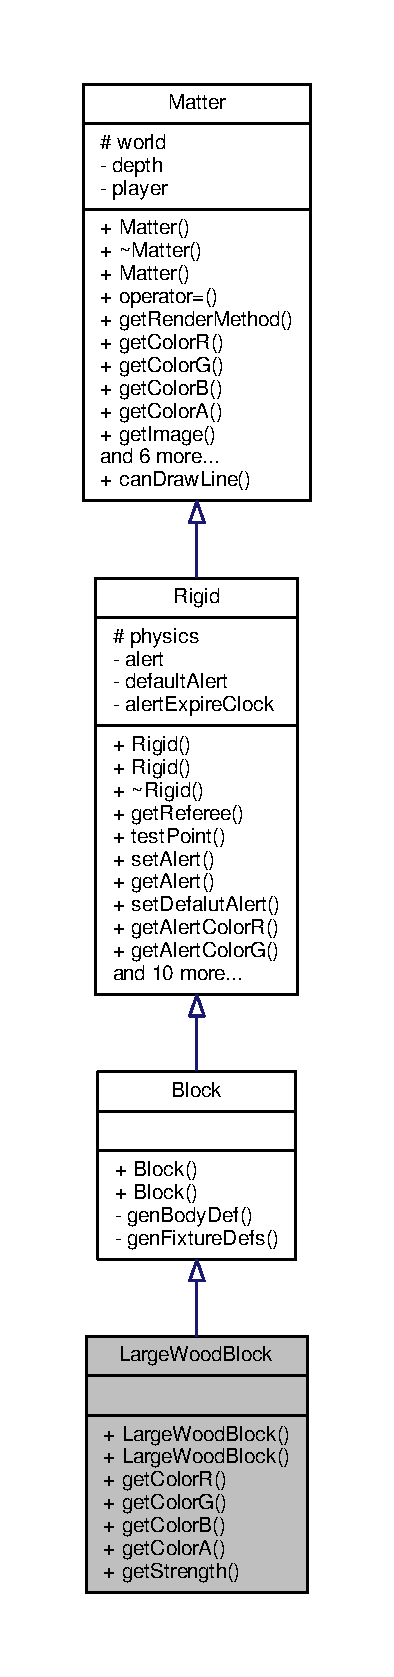
\includegraphics[height=550pt]{classLargeWoodBlock__inherit__graph}
\end{center}
\end{figure}


Collaboration diagram for Large\+Wood\+Block\+:\nopagebreak
\begin{figure}[H]
\begin{center}
\leavevmode
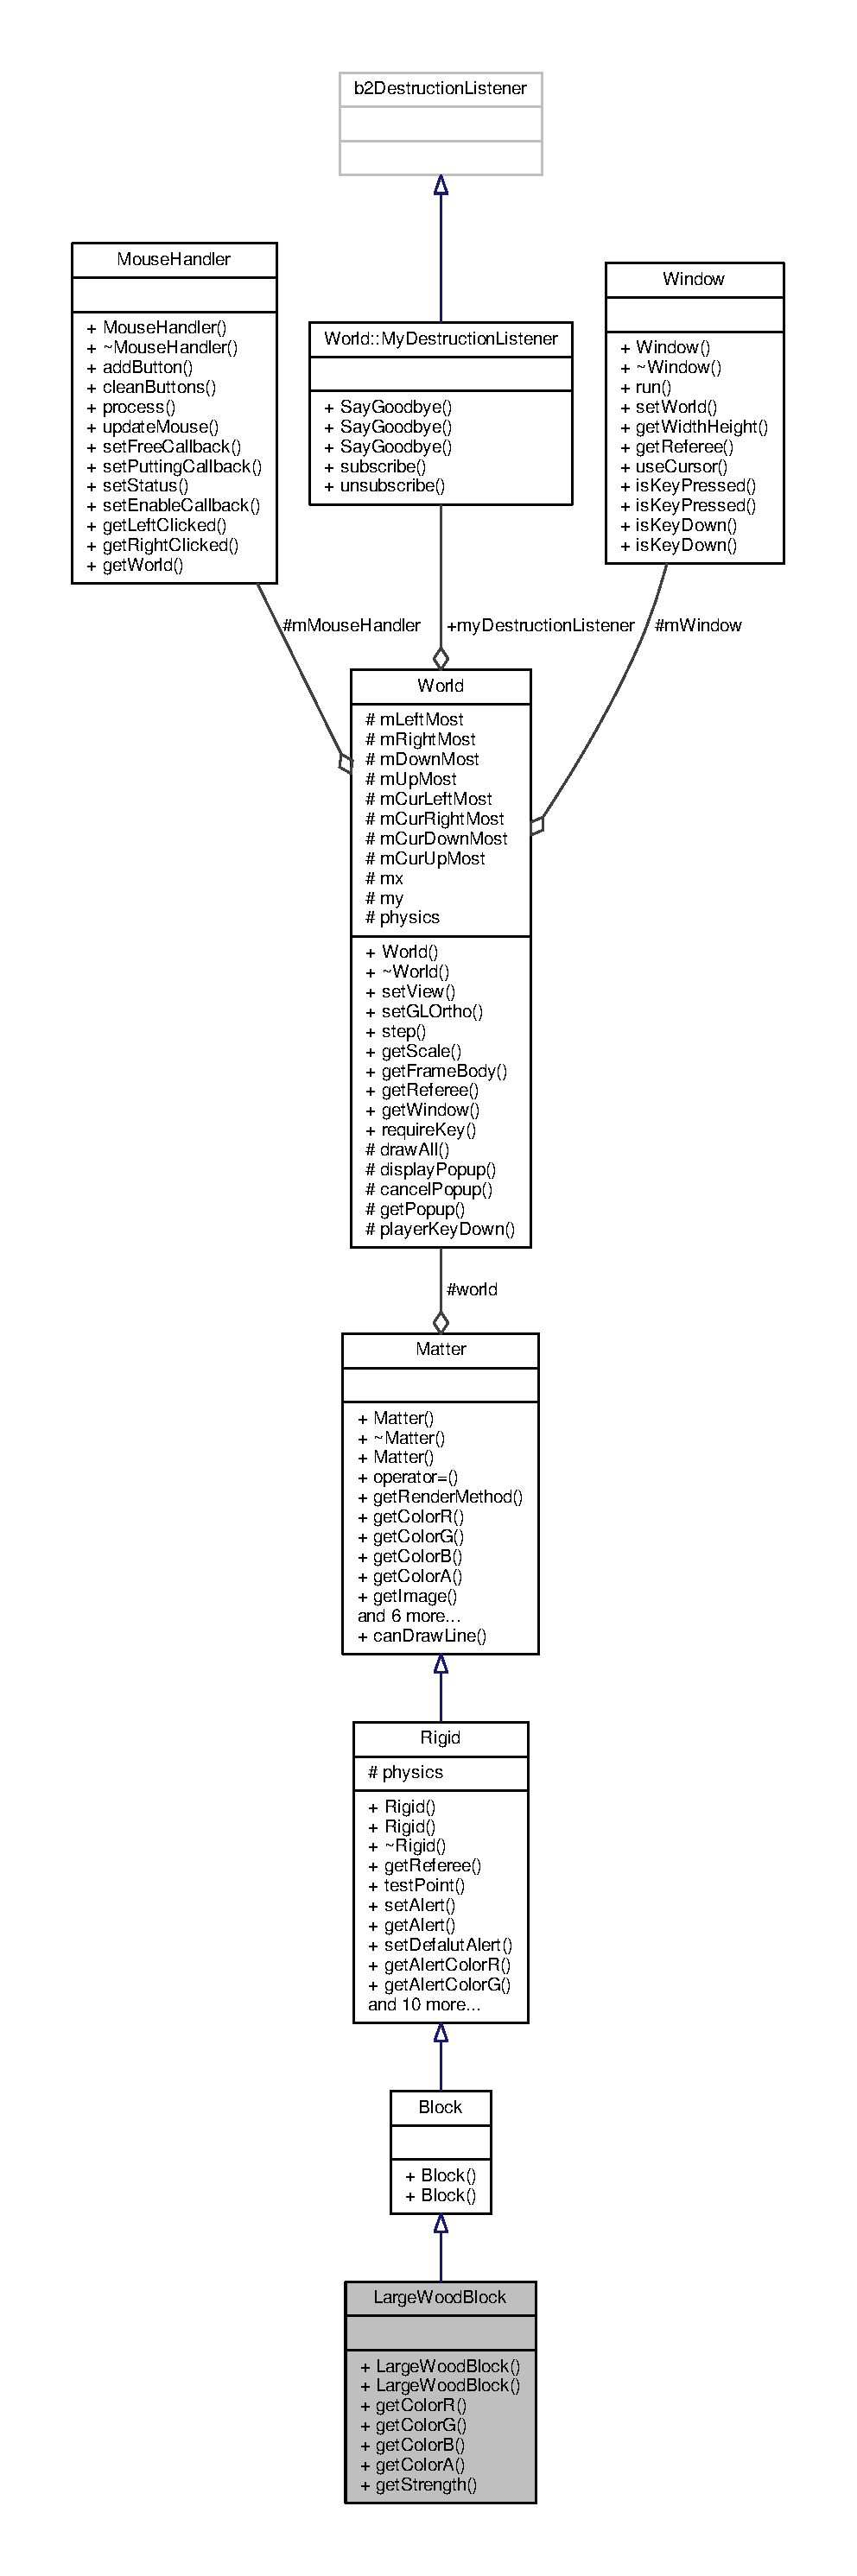
\includegraphics[height=550pt]{classLargeWoodBlock__coll__graph}
\end{center}
\end{figure}
\subsection*{Public Member Functions}
\begin{DoxyCompactItemize}
\item 
\hyperlink{classLargeWoodBlock_a4cc89f817ec63b73772111006cd6637e}{Large\+Wood\+Block} (\hyperlink{classWorld}{World} $\ast$\+\_\+world, b2\+Body $\ast$\hyperlink{image_8h_ab2d05693952610f937e5acb3c4a8fa1b}{b})
\item 
\hyperlink{classLargeWoodBlock_a508178e3bc340539a9b0e733eefebffb}{Large\+Wood\+Block} (\hyperlink{classWorld}{World} $\ast$\+\_\+world, float x, float y, float notused1=0, float notused2=0) noexcept
\item 
virtual float \hyperlink{classLargeWoodBlock_a3eeebdbf61b9f33a02b5c845f31ba428}{get\+Color\+R} () const override
\item 
virtual float \hyperlink{classLargeWoodBlock_ae422ccf33effdf80ee4bf7688de05b92}{get\+Color\+G} () const override
\item 
virtual float \hyperlink{classLargeWoodBlock_ac2499af4b661efeeee7662dff8af48f2}{get\+Color\+B} () const override
\item 
virtual float \hyperlink{classLargeWoodBlock_a74390f6c417c547b18db713696d2a12d}{get\+Color\+A} () const override
\item 
virtual float \hyperlink{classLargeWoodBlock_a445e21e6e8a723237616d3f7e0b6e1e0}{get\+Strength} () const override
\begin{DoxyCompactList}\small\item\em rigids are undestroyable by default \end{DoxyCompactList}\end{DoxyCompactItemize}
\subsection*{Additional Inherited Members}


\subsection{Detailed Description}
Dynamic 3\+X3 large wooden block Will Float. 

\subsection{Constructor \& Destructor Documentation}
\hypertarget{classLargeWoodBlock_a4cc89f817ec63b73772111006cd6637e}{}\index{Large\+Wood\+Block@{Large\+Wood\+Block}!Large\+Wood\+Block@{Large\+Wood\+Block}}
\index{Large\+Wood\+Block@{Large\+Wood\+Block}!Large\+Wood\+Block@{Large\+Wood\+Block}}
\subsubsection[{Large\+Wood\+Block}]{\setlength{\rightskip}{0pt plus 5cm}Large\+Wood\+Block\+::\+Large\+Wood\+Block (
\begin{DoxyParamCaption}
\item[{{\bf World} $\ast$}]{\+\_\+world, }
\item[{b2\+Body $\ast$}]{b}
\end{DoxyParamCaption}
)\hspace{0.3cm}{\ttfamily [inline]}}\label{classLargeWoodBlock_a4cc89f817ec63b73772111006cd6637e}
\hypertarget{classLargeWoodBlock_a508178e3bc340539a9b0e733eefebffb}{}\index{Large\+Wood\+Block@{Large\+Wood\+Block}!Large\+Wood\+Block@{Large\+Wood\+Block}}
\index{Large\+Wood\+Block@{Large\+Wood\+Block}!Large\+Wood\+Block@{Large\+Wood\+Block}}
\subsubsection[{Large\+Wood\+Block}]{\setlength{\rightskip}{0pt plus 5cm}Large\+Wood\+Block\+::\+Large\+Wood\+Block (
\begin{DoxyParamCaption}
\item[{{\bf World} $\ast$}]{\+\_\+world, }
\item[{float}]{x, }
\item[{float}]{y, }
\item[{float}]{notused1 = {\ttfamily 0}, }
\item[{float}]{notused2 = {\ttfamily 0}}
\end{DoxyParamCaption}
)\hspace{0.3cm}{\ttfamily [noexcept]}}\label{classLargeWoodBlock_a508178e3bc340539a9b0e733eefebffb}


\subsection{Member Function Documentation}
\hypertarget{classLargeWoodBlock_a74390f6c417c547b18db713696d2a12d}{}\index{Large\+Wood\+Block@{Large\+Wood\+Block}!get\+Color\+A@{get\+Color\+A}}
\index{get\+Color\+A@{get\+Color\+A}!Large\+Wood\+Block@{Large\+Wood\+Block}}
\subsubsection[{get\+Color\+A}]{\setlength{\rightskip}{0pt plus 5cm}virtual float Large\+Wood\+Block\+::get\+Color\+A (
\begin{DoxyParamCaption}
{}
\end{DoxyParamCaption}
) const\hspace{0.3cm}{\ttfamily [inline]}, {\ttfamily [override]}, {\ttfamily [virtual]}}\label{classLargeWoodBlock_a74390f6c417c547b18db713696d2a12d}


Reimplemented from \hyperlink{classMatter_aa44ee7ba48cb9a582a6f86e1e9e2ef38}{Matter}.

\hypertarget{classLargeWoodBlock_ac2499af4b661efeeee7662dff8af48f2}{}\index{Large\+Wood\+Block@{Large\+Wood\+Block}!get\+Color\+B@{get\+Color\+B}}
\index{get\+Color\+B@{get\+Color\+B}!Large\+Wood\+Block@{Large\+Wood\+Block}}
\subsubsection[{get\+Color\+B}]{\setlength{\rightskip}{0pt plus 5cm}virtual float Large\+Wood\+Block\+::get\+Color\+B (
\begin{DoxyParamCaption}
{}
\end{DoxyParamCaption}
) const\hspace{0.3cm}{\ttfamily [inline]}, {\ttfamily [override]}, {\ttfamily [virtual]}}\label{classLargeWoodBlock_ac2499af4b661efeeee7662dff8af48f2}


Reimplemented from \hyperlink{classMatter_af830da17da427c84c7f6deee4a91b3d4}{Matter}.

\hypertarget{classLargeWoodBlock_ae422ccf33effdf80ee4bf7688de05b92}{}\index{Large\+Wood\+Block@{Large\+Wood\+Block}!get\+Color\+G@{get\+Color\+G}}
\index{get\+Color\+G@{get\+Color\+G}!Large\+Wood\+Block@{Large\+Wood\+Block}}
\subsubsection[{get\+Color\+G}]{\setlength{\rightskip}{0pt plus 5cm}virtual float Large\+Wood\+Block\+::get\+Color\+G (
\begin{DoxyParamCaption}
{}
\end{DoxyParamCaption}
) const\hspace{0.3cm}{\ttfamily [inline]}, {\ttfamily [override]}, {\ttfamily [virtual]}}\label{classLargeWoodBlock_ae422ccf33effdf80ee4bf7688de05b92}


Reimplemented from \hyperlink{classMatter_aa3fcdc82f788fbf873ec3ff4808f614a}{Matter}.

\hypertarget{classLargeWoodBlock_a3eeebdbf61b9f33a02b5c845f31ba428}{}\index{Large\+Wood\+Block@{Large\+Wood\+Block}!get\+Color\+R@{get\+Color\+R}}
\index{get\+Color\+R@{get\+Color\+R}!Large\+Wood\+Block@{Large\+Wood\+Block}}
\subsubsection[{get\+Color\+R}]{\setlength{\rightskip}{0pt plus 5cm}virtual float Large\+Wood\+Block\+::get\+Color\+R (
\begin{DoxyParamCaption}
{}
\end{DoxyParamCaption}
) const\hspace{0.3cm}{\ttfamily [inline]}, {\ttfamily [override]}, {\ttfamily [virtual]}}\label{classLargeWoodBlock_a3eeebdbf61b9f33a02b5c845f31ba428}


Reimplemented from \hyperlink{classMatter_a926d246584228c3e3b102dbfd42036ec}{Matter}.

\hypertarget{classLargeWoodBlock_a445e21e6e8a723237616d3f7e0b6e1e0}{}\index{Large\+Wood\+Block@{Large\+Wood\+Block}!get\+Strength@{get\+Strength}}
\index{get\+Strength@{get\+Strength}!Large\+Wood\+Block@{Large\+Wood\+Block}}
\subsubsection[{get\+Strength}]{\setlength{\rightskip}{0pt plus 5cm}virtual float Large\+Wood\+Block\+::get\+Strength (
\begin{DoxyParamCaption}
{}
\end{DoxyParamCaption}
) const\hspace{0.3cm}{\ttfamily [inline]}, {\ttfamily [override]}, {\ttfamily [virtual]}}\label{classLargeWoodBlock_a445e21e6e8a723237616d3f7e0b6e1e0}


rigids are undestroyable by default 



Reimplemented from \hyperlink{classRigid_aac83bf941605a8cbccf06a5d4b200fee}{Rigid}.



The documentation for this class was generated from the following files\+:\begin{DoxyCompactItemize}
\item 
\hyperlink{matter_8h}{matter.\+h}\item 
\hyperlink{matter_8cpp}{matter.\+cpp}\end{DoxyCompactItemize}

\hypertarget{classLaunchCallback}{}\section{Launch\+Callback Class Reference}
\label{classLaunchCallback}\index{Launch\+Callback@{Launch\+Callback}}


Inheritance diagram for Launch\+Callback\+:\nopagebreak
\begin{figure}[H]
\begin{center}
\leavevmode
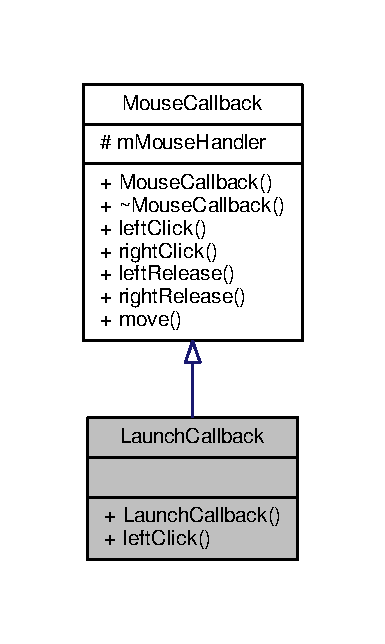
\includegraphics[width=185pt]{classLaunchCallback__inherit__graph}
\end{center}
\end{figure}


Collaboration diagram for Launch\+Callback\+:\nopagebreak
\begin{figure}[H]
\begin{center}
\leavevmode
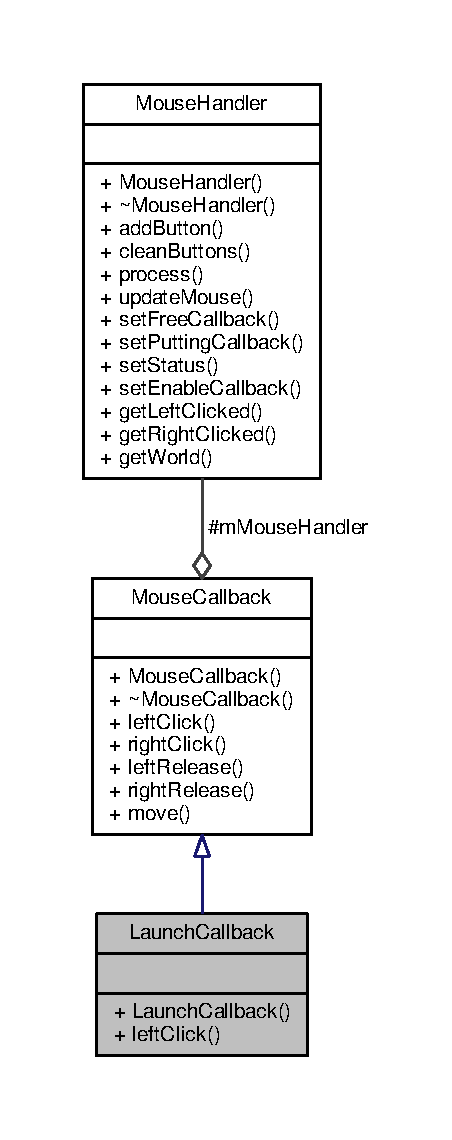
\includegraphics[width=217pt]{classLaunchCallback__coll__graph}
\end{center}
\end{figure}
\subsection*{Public Member Functions}
\begin{DoxyCompactItemize}
\item 
\hyperlink{classLaunchCallback_a51e647404646b4270f6fcc9c375097e7}{Launch\+Callback} (\hyperlink{classMouseHandler}{Mouse\+Handler} $\ast$\+\_\+handler)
\item 
void \hyperlink{classLaunchCallback_ab86a248b06b3c32bd26cb5bd9aa60745}{left\+Click} (float, float)
\end{DoxyCompactItemize}
\subsection*{Additional Inherited Members}


\subsection{Constructor \& Destructor Documentation}
\hypertarget{classLaunchCallback_a51e647404646b4270f6fcc9c375097e7}{}\index{Launch\+Callback@{Launch\+Callback}!Launch\+Callback@{Launch\+Callback}}
\index{Launch\+Callback@{Launch\+Callback}!Launch\+Callback@{Launch\+Callback}}
\subsubsection[{Launch\+Callback}]{\setlength{\rightskip}{0pt plus 5cm}Launch\+Callback\+::\+Launch\+Callback (
\begin{DoxyParamCaption}
\item[{{\bf Mouse\+Handler} $\ast$}]{\+\_\+handler}
\end{DoxyParamCaption}
)\hspace{0.3cm}{\ttfamily [inline]}}\label{classLaunchCallback_a51e647404646b4270f6fcc9c375097e7}


\subsection{Member Function Documentation}
\hypertarget{classLaunchCallback_ab86a248b06b3c32bd26cb5bd9aa60745}{}\index{Launch\+Callback@{Launch\+Callback}!left\+Click@{left\+Click}}
\index{left\+Click@{left\+Click}!Launch\+Callback@{Launch\+Callback}}
\subsubsection[{left\+Click}]{\setlength{\rightskip}{0pt plus 5cm}void Launch\+Callback\+::left\+Click (
\begin{DoxyParamCaption}
\item[{float}]{, }
\item[{float}]{}
\end{DoxyParamCaption}
)\hspace{0.3cm}{\ttfamily [inline]}, {\ttfamily [virtual]}}\label{classLaunchCallback_ab86a248b06b3c32bd26cb5bd9aa60745}


Reimplemented from \hyperlink{classMouseCallback_a5ae88358471f1b48e3f6a730aaf0ba13}{Mouse\+Callback}.



The documentation for this class was generated from the following file\+:\begin{DoxyCompactItemize}
\item 
\hyperlink{world_8cpp}{world.\+cpp}\end{DoxyCompactItemize}

\hypertarget{classDraggingCallback_1_1LocalListener}{}\section{Dragging\+Callback\+:\+:Local\+Listener Class Reference}
\label{classDraggingCallback_1_1LocalListener}\index{Dragging\+Callback\+::\+Local\+Listener@{Dragging\+Callback\+::\+Local\+Listener}}


{\ttfamily \#include $<$mousecallback.\+h$>$}



Inheritance diagram for Dragging\+Callback\+:\+:Local\+Listener\+:\nopagebreak
\begin{figure}[H]
\begin{center}
\leavevmode
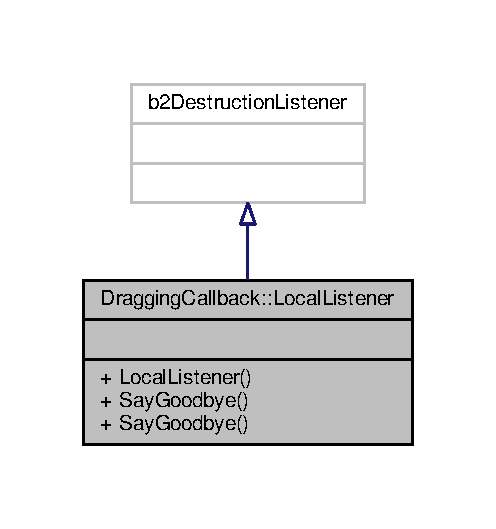
\includegraphics[width=238pt]{classDraggingCallback_1_1LocalListener__inherit__graph}
\end{center}
\end{figure}


Collaboration diagram for Dragging\+Callback\+:\+:Local\+Listener\+:\nopagebreak
\begin{figure}[H]
\begin{center}
\leavevmode
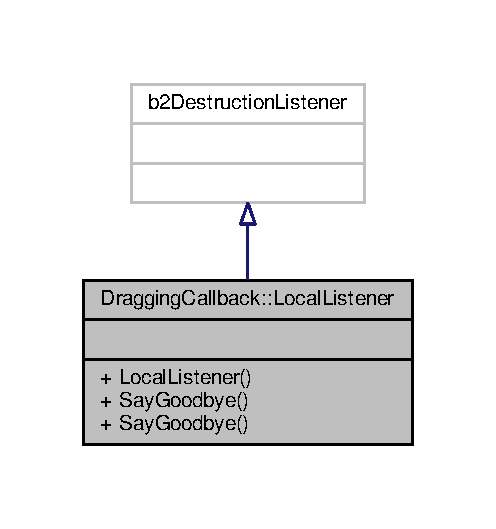
\includegraphics[width=238pt]{classDraggingCallback_1_1LocalListener__coll__graph}
\end{center}
\end{figure}
\subsection*{Public Member Functions}
\begin{DoxyCompactItemize}
\item 
\hyperlink{classDraggingCallback_1_1LocalListener_aa4ded3e2d1d7f0be56de96086fa488bc}{Local\+Listener} (Joint\+Pointer \&\+\_\+joint)
\item 
void \hyperlink{classDraggingCallback_1_1LocalListener_aedc2cc229bce114eda98ee8d470acca9}{Say\+Goodbye} (b2\+Joint $\ast$\+\_\+joint) override
\item 
void \hyperlink{classDraggingCallback_1_1LocalListener_a9cc8d876dc60495f9c8ba0c328db31d5}{Say\+Goodbye} (b2\+Fixture $\ast$) override
\end{DoxyCompactItemize}


\subsection{Constructor \& Destructor Documentation}
\hypertarget{classDraggingCallback_1_1LocalListener_aa4ded3e2d1d7f0be56de96086fa488bc}{}\index{Dragging\+Callback\+::\+Local\+Listener@{Dragging\+Callback\+::\+Local\+Listener}!Local\+Listener@{Local\+Listener}}
\index{Local\+Listener@{Local\+Listener}!Dragging\+Callback\+::\+Local\+Listener@{Dragging\+Callback\+::\+Local\+Listener}}
\subsubsection[{Local\+Listener}]{\setlength{\rightskip}{0pt plus 5cm}Dragging\+Callback\+::\+Local\+Listener\+::\+Local\+Listener (
\begin{DoxyParamCaption}
\item[{Joint\+Pointer \&}]{\+\_\+joint}
\end{DoxyParamCaption}
)\hspace{0.3cm}{\ttfamily [inline]}}\label{classDraggingCallback_1_1LocalListener_aa4ded3e2d1d7f0be56de96086fa488bc}


\subsection{Member Function Documentation}
\hypertarget{classDraggingCallback_1_1LocalListener_aedc2cc229bce114eda98ee8d470acca9}{}\index{Dragging\+Callback\+::\+Local\+Listener@{Dragging\+Callback\+::\+Local\+Listener}!Say\+Goodbye@{Say\+Goodbye}}
\index{Say\+Goodbye@{Say\+Goodbye}!Dragging\+Callback\+::\+Local\+Listener@{Dragging\+Callback\+::\+Local\+Listener}}
\subsubsection[{Say\+Goodbye}]{\setlength{\rightskip}{0pt plus 5cm}void Dragging\+Callback\+::\+Local\+Listener\+::\+Say\+Goodbye (
\begin{DoxyParamCaption}
\item[{b2\+Joint $\ast$}]{\+\_\+joint}
\end{DoxyParamCaption}
)\hspace{0.3cm}{\ttfamily [inline]}, {\ttfamily [override]}}\label{classDraggingCallback_1_1LocalListener_aedc2cc229bce114eda98ee8d470acca9}
\hypertarget{classDraggingCallback_1_1LocalListener_a9cc8d876dc60495f9c8ba0c328db31d5}{}\index{Dragging\+Callback\+::\+Local\+Listener@{Dragging\+Callback\+::\+Local\+Listener}!Say\+Goodbye@{Say\+Goodbye}}
\index{Say\+Goodbye@{Say\+Goodbye}!Dragging\+Callback\+::\+Local\+Listener@{Dragging\+Callback\+::\+Local\+Listener}}
\subsubsection[{Say\+Goodbye}]{\setlength{\rightskip}{0pt plus 5cm}void Dragging\+Callback\+::\+Local\+Listener\+::\+Say\+Goodbye (
\begin{DoxyParamCaption}
\item[{b2\+Fixture $\ast$}]{}
\end{DoxyParamCaption}
)\hspace{0.3cm}{\ttfamily [inline]}, {\ttfamily [override]}}\label{classDraggingCallback_1_1LocalListener_a9cc8d876dc60495f9c8ba0c328db31d5}


The documentation for this class was generated from the following file\+:\begin{DoxyCompactItemize}
\item 
\hyperlink{mousecallback_8h}{mousecallback.\+h}\end{DoxyCompactItemize}

\hypertarget{classMainWorld}{}\section{Main\+World Class Reference}
\label{classMainWorld}\index{Main\+World@{Main\+World}}


This world is the main scenery of the game.  




{\ttfamily \#include $<$world.\+h$>$}



Inheritance diagram for Main\+World\+:
\nopagebreak
\begin{figure}[H]
\begin{center}
\leavevmode
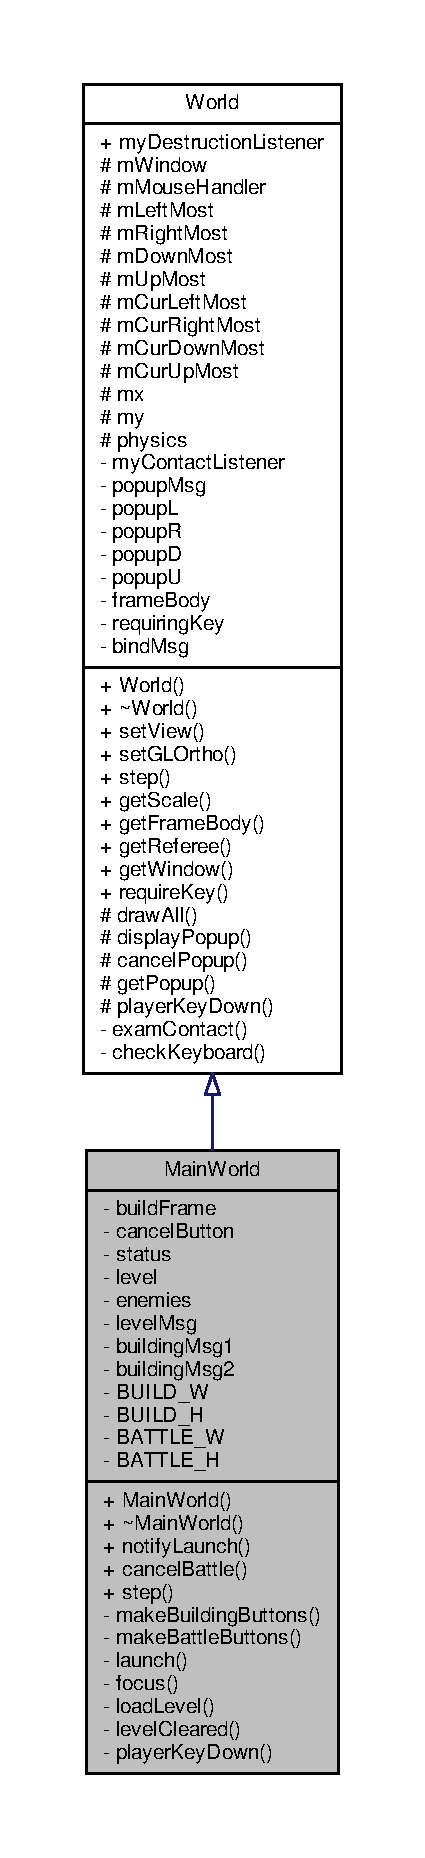
\includegraphics[height=550pt]{classMainWorld__inherit__graph}
\end{center}
\end{figure}


Collaboration diagram for Main\+World\+:
\nopagebreak
\begin{figure}[H]
\begin{center}
\leavevmode
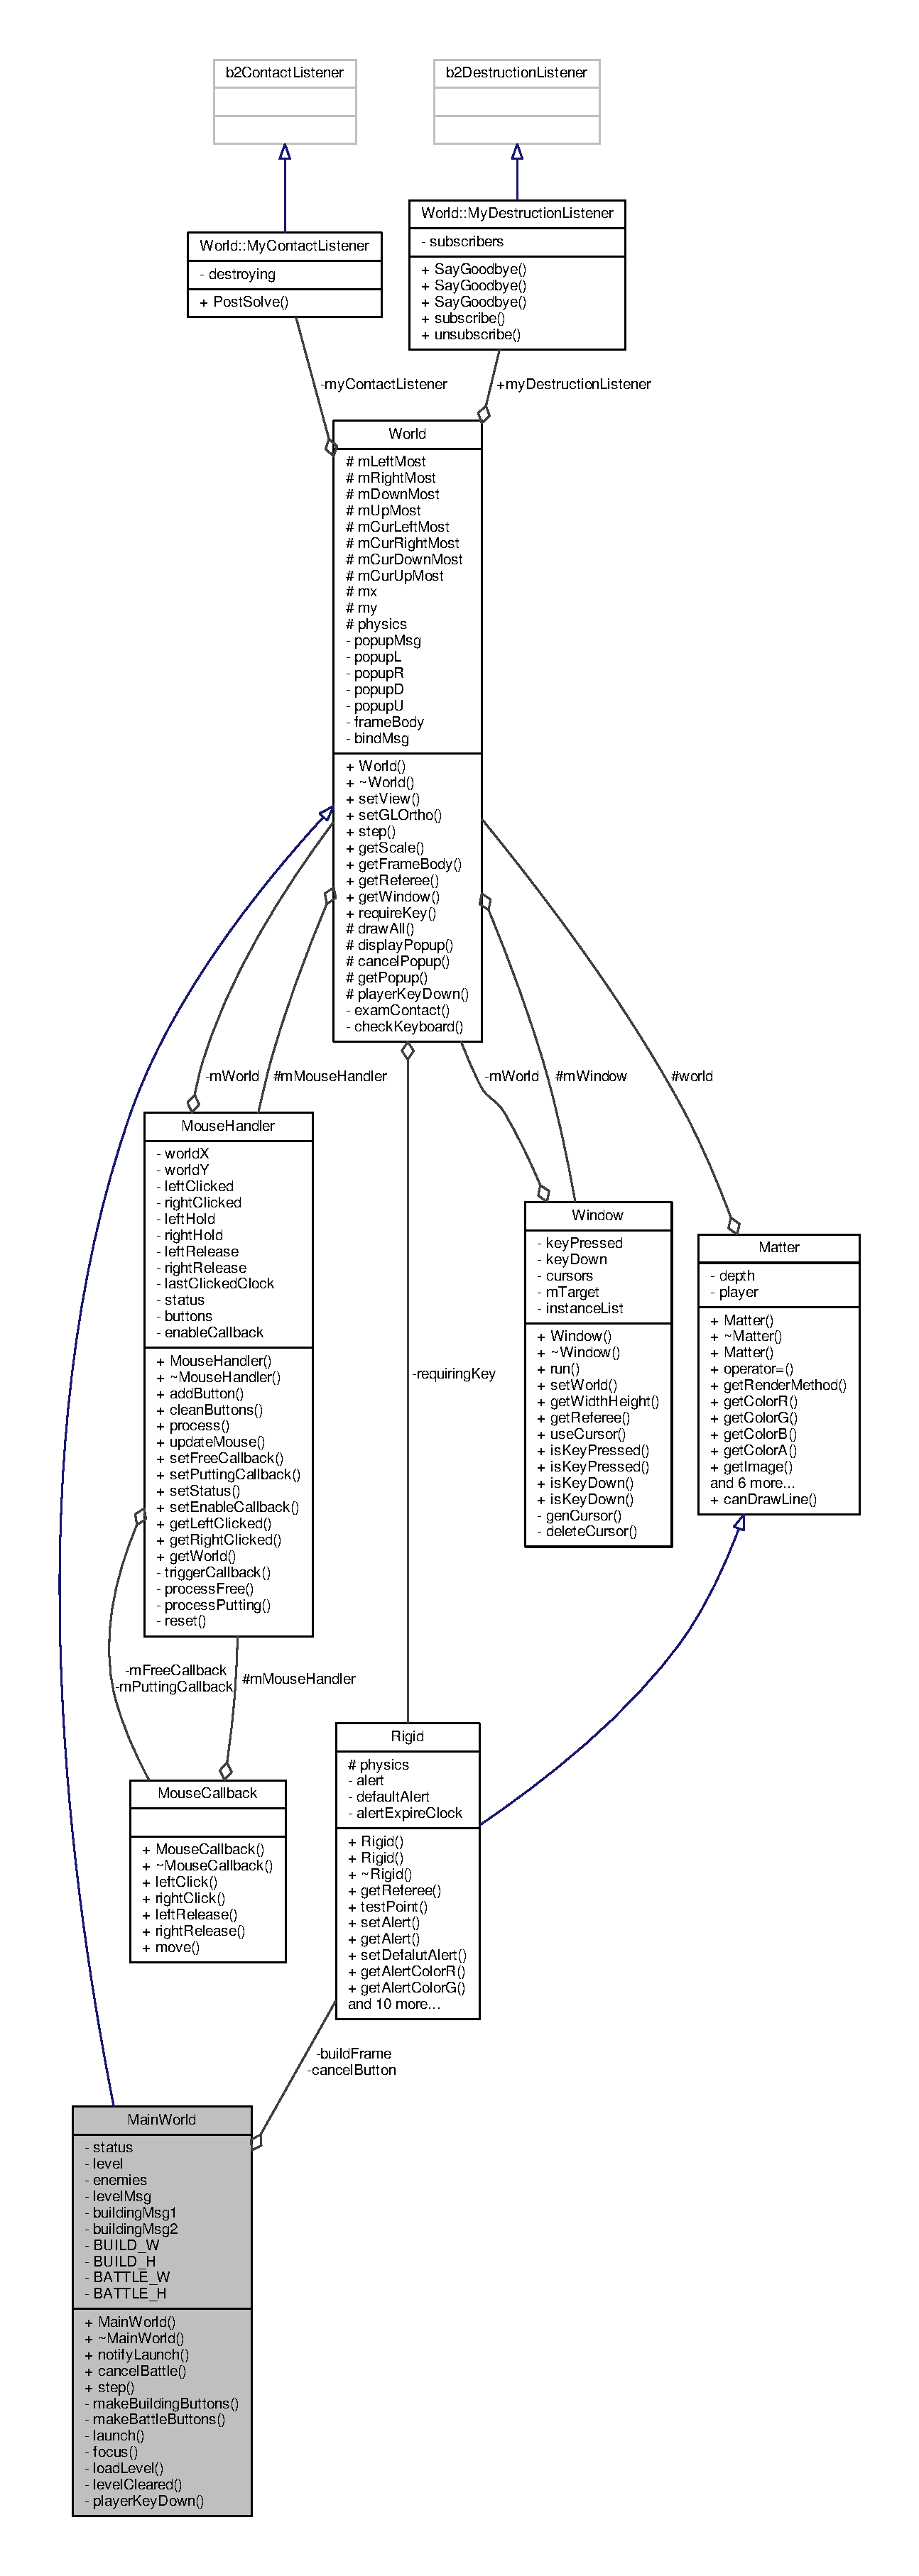
\includegraphics[height=550pt]{classMainWorld__coll__graph}
\end{center}
\end{figure}
\subsection*{Public Types}
\begin{DoxyCompactItemize}
\item 
enum \hyperlink{classMainWorld_ab0b1d1d54026f907ddc7fcc858ea48f3}{World\+Status} \{ \hyperlink{classMainWorld_ab0b1d1d54026f907ddc7fcc858ea48f3af96d574a62f6b5920f3fad277d995fb7}{S\+T\+A\+T\+U\+S\+\_\+\+B\+U\+I\+L\+D\+I\+N\+G} = 0, 
\hyperlink{classMainWorld_ab0b1d1d54026f907ddc7fcc858ea48f3a56955ec18d3375dec123f1d3d65c7393}{S\+T\+A\+T\+U\+S\+\_\+\+B\+A\+T\+T\+L\+E} = 1, 
\hyperlink{classMainWorld_ab0b1d1d54026f907ddc7fcc858ea48f3adf5d74eb401b14e4f5f33d375d6ffedd}{S\+T\+A\+T\+U\+S\+\_\+\+N\+O\+T\+I\+F\+Y\+\_\+\+L\+A\+U\+N\+C\+H} = 2, 
\hyperlink{classMainWorld_ab0b1d1d54026f907ddc7fcc858ea48f3a0adce04cf20701967507ab5eb64e2011}{S\+T\+A\+T\+U\+S\+\_\+\+C\+A\+N\+C\+E\+L\+\_\+\+B\+A\+T\+T\+L\+E} = 3
 \}
\end{DoxyCompactItemize}
\subsection*{Public Member Functions}
\begin{DoxyCompactItemize}
\item 
\hyperlink{classMainWorld_a46e56e826f563bf0255ad7e44944d286}{Main\+World} (int \+\_\+level=0)
\item 
\hyperlink{classMainWorld_ace9d329c017b003879831dcd8295cfe0}{$\sim$\+Main\+World} ()
\item 
void \hyperlink{classMainWorld_a7b7a15580a43911c7252d179b320bddd}{notify\+Launch} ()
\begin{DoxyCompactList}\small\item\em Switch from building to battle in the next round. \end{DoxyCompactList}\item 
void \hyperlink{classMainWorld_a223280718d44259c485fbbaaf74c34e5}{cancel\+Battle} ()
\begin{DoxyCompactList}\small\item\em Cancel battle in the next round. \end{DoxyCompactList}\item 
void \hyperlink{classMainWorld_a8ac7fe4b17bb3ca29a0382b93a24731e}{step} () override
\begin{DoxyCompactList}\small\item\em Run next simulation step. \end{DoxyCompactList}\end{DoxyCompactItemize}
\subsection*{Private Member Functions}
\begin{DoxyCompactItemize}
\item 
void \hyperlink{classMainWorld_a4c59edbfc967da60dd2eee28280434d1}{make\+Building\+Buttons} ()
\begin{DoxyCompactList}\small\item\em This is called during construction. \end{DoxyCompactList}\item 
void \hyperlink{classMainWorld_a34ff55bf7bec578a3eada27017973e77}{make\+Battle\+Buttons} ()
\item 
void \hyperlink{classMainWorld_ace8b3e2cbb1c1cb8d2a3fe149dabe734}{launch} ()
\begin{DoxyCompactList}\small\item\em Switch from building to battle. \end{DoxyCompactList}\item 
void \hyperlink{classMainWorld_a00895e34e30d1299e9d6d3aef874c2eb}{focus} ()
\begin{DoxyCompactList}\small\item\em Focus on the ship built by players. \end{DoxyCompactList}\item 
bool \hyperlink{classMainWorld_a4011961e71f2129896ce5248fe5ccf20}{load\+Level} ()
\item 
bool \hyperlink{classMainWorld_a27b5623f73157f016b93ea0e27cd3166}{level\+Cleared} () const 
\item 
bool \hyperlink{classMainWorld_a8e17a525de341eda83c8bcb1020e779b}{player\+Key\+Down} (int p, int key) override
\begin{DoxyCompactList}\small\item\em Is player p\textquotesingle{}s key down? \end{DoxyCompactList}\end{DoxyCompactItemize}
\subsection*{Private Attributes}
\begin{DoxyCompactItemize}
\item 
\hyperlink{classRigid}{Rigid} $\ast$ \hyperlink{classMainWorld_a10e4e51760423fa95cc57f4f5f8f5b76}{build\+Frame}
\item 
\hyperlink{classRigid}{Rigid} $\ast$ \hyperlink{classMainWorld_a44391b2d794f460d9e9898716f7c00e8}{cancel\+Button}
\item 
\hyperlink{classMainWorld_ab0b1d1d54026f907ddc7fcc858ea48f3}{World\+Status} \hyperlink{classMainWorld_a9769c3d0399e2d8a8176c0c21762b1eb}{status}
\item 
int \hyperlink{classMainWorld_a858b57e7a6e32e4f771c66b87cfac1d7}{level}
\item 
std\+::unordered\+\_\+map$<$ int, \hyperlink{classEnemy}{Enemy} $\ast$ $>$ \hyperlink{classMainWorld_a47830d0b4f72482d07985b94b982f4b3}{enemies}
\item 
std\+::string \hyperlink{classMainWorld_a0d1545c344c83a85d56597b8e582a6db}{level\+Msg}
\item 
const std\+::string \hyperlink{classMainWorld_a12fc771468255ea67138459b8f80bb95}{building\+Msg1}
\item 
const std\+::string \hyperlink{classMainWorld_ac33f26e815fc9f69e5119843dfc2b987}{building\+Msg2}
\end{DoxyCompactItemize}
\subsection*{Static Private Attributes}
\begin{DoxyCompactItemize}
\item 
static constexpr float \hyperlink{classMainWorld_a92c8b34eec78a999312c4b1d982d5f0c}{B\+U\+I\+L\+D\+\_\+\+W} = 30.\+0f
\item 
static constexpr float \hyperlink{classMainWorld_abb38bf72b8a3c5ff6df3a43c7ebfba25}{B\+U\+I\+L\+D\+\_\+\+H} = 23.\+0f
\item 
static constexpr float \hyperlink{classMainWorld_a58ef88e1b0a8c840090a44ceb9917f8a}{B\+A\+T\+T\+L\+E\+\_\+\+W} = 180.\+0f
\item 
static constexpr float \hyperlink{classMainWorld_aa2bb1e5ed0ea5b97b36addf18ec1b37c}{B\+A\+T\+T\+L\+E\+\_\+\+H} = 60.\+0f
\end{DoxyCompactItemize}
\subsection*{Additional Inherited Members}


\subsection{Detailed Description}
This world is the main scenery of the game. 

Players first build a ship in a limited area. When clicked Battle, he will be set free and play. 

\subsection{Member Enumeration Documentation}
\hypertarget{classMainWorld_ab0b1d1d54026f907ddc7fcc858ea48f3}{}\index{Main\+World@{Main\+World}!World\+Status@{World\+Status}}
\index{World\+Status@{World\+Status}!Main\+World@{Main\+World}}
\subsubsection[{World\+Status}]{\setlength{\rightskip}{0pt plus 5cm}enum {\bf Main\+World\+::\+World\+Status}}\label{classMainWorld_ab0b1d1d54026f907ddc7fcc858ea48f3}
\begin{Desc}
\item[Enumerator]\par
\begin{description}
\index{S\+T\+A\+T\+U\+S\+\_\+\+B\+U\+I\+L\+D\+I\+N\+G@{S\+T\+A\+T\+U\+S\+\_\+\+B\+U\+I\+L\+D\+I\+N\+G}!Main\+World@{Main\+World}}\index{Main\+World@{Main\+World}!S\+T\+A\+T\+U\+S\+\_\+\+B\+U\+I\+L\+D\+I\+N\+G@{S\+T\+A\+T\+U\+S\+\_\+\+B\+U\+I\+L\+D\+I\+N\+G}}\item[{\em 
\hypertarget{classMainWorld_ab0b1d1d54026f907ddc7fcc858ea48f3af96d574a62f6b5920f3fad277d995fb7}{}S\+T\+A\+T\+U\+S\+\_\+\+B\+U\+I\+L\+D\+I\+N\+G\label{classMainWorld_ab0b1d1d54026f907ddc7fcc858ea48f3af96d574a62f6b5920f3fad277d995fb7}
}]\index{S\+T\+A\+T\+U\+S\+\_\+\+B\+A\+T\+T\+L\+E@{S\+T\+A\+T\+U\+S\+\_\+\+B\+A\+T\+T\+L\+E}!Main\+World@{Main\+World}}\index{Main\+World@{Main\+World}!S\+T\+A\+T\+U\+S\+\_\+\+B\+A\+T\+T\+L\+E@{S\+T\+A\+T\+U\+S\+\_\+\+B\+A\+T\+T\+L\+E}}\item[{\em 
\hypertarget{classMainWorld_ab0b1d1d54026f907ddc7fcc858ea48f3a56955ec18d3375dec123f1d3d65c7393}{}S\+T\+A\+T\+U\+S\+\_\+\+B\+A\+T\+T\+L\+E\label{classMainWorld_ab0b1d1d54026f907ddc7fcc858ea48f3a56955ec18d3375dec123f1d3d65c7393}
}]\index{S\+T\+A\+T\+U\+S\+\_\+\+N\+O\+T\+I\+F\+Y\+\_\+\+L\+A\+U\+N\+C\+H@{S\+T\+A\+T\+U\+S\+\_\+\+N\+O\+T\+I\+F\+Y\+\_\+\+L\+A\+U\+N\+C\+H}!Main\+World@{Main\+World}}\index{Main\+World@{Main\+World}!S\+T\+A\+T\+U\+S\+\_\+\+N\+O\+T\+I\+F\+Y\+\_\+\+L\+A\+U\+N\+C\+H@{S\+T\+A\+T\+U\+S\+\_\+\+N\+O\+T\+I\+F\+Y\+\_\+\+L\+A\+U\+N\+C\+H}}\item[{\em 
\hypertarget{classMainWorld_ab0b1d1d54026f907ddc7fcc858ea48f3adf5d74eb401b14e4f5f33d375d6ffedd}{}S\+T\+A\+T\+U\+S\+\_\+\+N\+O\+T\+I\+F\+Y\+\_\+\+L\+A\+U\+N\+C\+H\label{classMainWorld_ab0b1d1d54026f907ddc7fcc858ea48f3adf5d74eb401b14e4f5f33d375d6ffedd}
}]\index{S\+T\+A\+T\+U\+S\+\_\+\+C\+A\+N\+C\+E\+L\+\_\+\+B\+A\+T\+T\+L\+E@{S\+T\+A\+T\+U\+S\+\_\+\+C\+A\+N\+C\+E\+L\+\_\+\+B\+A\+T\+T\+L\+E}!Main\+World@{Main\+World}}\index{Main\+World@{Main\+World}!S\+T\+A\+T\+U\+S\+\_\+\+C\+A\+N\+C\+E\+L\+\_\+\+B\+A\+T\+T\+L\+E@{S\+T\+A\+T\+U\+S\+\_\+\+C\+A\+N\+C\+E\+L\+\_\+\+B\+A\+T\+T\+L\+E}}\item[{\em 
\hypertarget{classMainWorld_ab0b1d1d54026f907ddc7fcc858ea48f3a0adce04cf20701967507ab5eb64e2011}{}S\+T\+A\+T\+U\+S\+\_\+\+C\+A\+N\+C\+E\+L\+\_\+\+B\+A\+T\+T\+L\+E\label{classMainWorld_ab0b1d1d54026f907ddc7fcc858ea48f3a0adce04cf20701967507ab5eb64e2011}
}]\end{description}
\end{Desc}


\subsection{Constructor \& Destructor Documentation}
\hypertarget{classMainWorld_a46e56e826f563bf0255ad7e44944d286}{}\index{Main\+World@{Main\+World}!Main\+World@{Main\+World}}
\index{Main\+World@{Main\+World}!Main\+World@{Main\+World}}
\subsubsection[{Main\+World}]{\setlength{\rightskip}{0pt plus 5cm}Main\+World\+::\+Main\+World (
\begin{DoxyParamCaption}
\item[{int}]{\+\_\+level = {\ttfamily 0}}
\end{DoxyParamCaption}
)}\label{classMainWorld_a46e56e826f563bf0255ad7e44944d286}
\hypertarget{classMainWorld_ace9d329c017b003879831dcd8295cfe0}{}\index{Main\+World@{Main\+World}!````~Main\+World@{$\sim$\+Main\+World}}
\index{````~Main\+World@{$\sim$\+Main\+World}!Main\+World@{Main\+World}}
\subsubsection[{$\sim$\+Main\+World}]{\setlength{\rightskip}{0pt plus 5cm}Main\+World\+::$\sim$\+Main\+World (
\begin{DoxyParamCaption}
{}
\end{DoxyParamCaption}
)}\label{classMainWorld_ace9d329c017b003879831dcd8295cfe0}


\subsection{Member Function Documentation}
\hypertarget{classMainWorld_a223280718d44259c485fbbaaf74c34e5}{}\index{Main\+World@{Main\+World}!cancel\+Battle@{cancel\+Battle}}
\index{cancel\+Battle@{cancel\+Battle}!Main\+World@{Main\+World}}
\subsubsection[{cancel\+Battle}]{\setlength{\rightskip}{0pt plus 5cm}void Main\+World\+::cancel\+Battle (
\begin{DoxyParamCaption}
{}
\end{DoxyParamCaption}
)\hspace{0.3cm}{\ttfamily [inline]}}\label{classMainWorld_a223280718d44259c485fbbaaf74c34e5}


Cancel battle in the next round. 

\hypertarget{classMainWorld_a00895e34e30d1299e9d6d3aef874c2eb}{}\index{Main\+World@{Main\+World}!focus@{focus}}
\index{focus@{focus}!Main\+World@{Main\+World}}
\subsubsection[{focus}]{\setlength{\rightskip}{0pt plus 5cm}void Main\+World\+::focus (
\begin{DoxyParamCaption}
{}
\end{DoxyParamCaption}
)\hspace{0.3cm}{\ttfamily [private]}}\label{classMainWorld_a00895e34e30d1299e9d6d3aef874c2eb}


Focus on the ship built by players. 

\hypertarget{classMainWorld_ace8b3e2cbb1c1cb8d2a3fe149dabe734}{}\index{Main\+World@{Main\+World}!launch@{launch}}
\index{launch@{launch}!Main\+World@{Main\+World}}
\subsubsection[{launch}]{\setlength{\rightskip}{0pt plus 5cm}void Main\+World\+::launch (
\begin{DoxyParamCaption}
{}
\end{DoxyParamCaption}
)\hspace{0.3cm}{\ttfamily [private]}}\label{classMainWorld_ace8b3e2cbb1c1cb8d2a3fe149dabe734}


Switch from building to battle. 

\hypertarget{classMainWorld_a27b5623f73157f016b93ea0e27cd3166}{}\index{Main\+World@{Main\+World}!level\+Cleared@{level\+Cleared}}
\index{level\+Cleared@{level\+Cleared}!Main\+World@{Main\+World}}
\subsubsection[{level\+Cleared}]{\setlength{\rightskip}{0pt plus 5cm}bool Main\+World\+::level\+Cleared (
\begin{DoxyParamCaption}
{}
\end{DoxyParamCaption}
) const\hspace{0.3cm}{\ttfamily [private]}}\label{classMainWorld_a27b5623f73157f016b93ea0e27cd3166}
\hypertarget{classMainWorld_a4011961e71f2129896ce5248fe5ccf20}{}\index{Main\+World@{Main\+World}!load\+Level@{load\+Level}}
\index{load\+Level@{load\+Level}!Main\+World@{Main\+World}}
\subsubsection[{load\+Level}]{\setlength{\rightskip}{0pt plus 5cm}bool Main\+World\+::load\+Level (
\begin{DoxyParamCaption}
{}
\end{DoxyParamCaption}
)\hspace{0.3cm}{\ttfamily [private]}}\label{classMainWorld_a4011961e71f2129896ce5248fe5ccf20}
\hypertarget{classMainWorld_a34ff55bf7bec578a3eada27017973e77}{}\index{Main\+World@{Main\+World}!make\+Battle\+Buttons@{make\+Battle\+Buttons}}
\index{make\+Battle\+Buttons@{make\+Battle\+Buttons}!Main\+World@{Main\+World}}
\subsubsection[{make\+Battle\+Buttons}]{\setlength{\rightskip}{0pt plus 5cm}void Main\+World\+::make\+Battle\+Buttons (
\begin{DoxyParamCaption}
{}
\end{DoxyParamCaption}
)\hspace{0.3cm}{\ttfamily [private]}}\label{classMainWorld_a34ff55bf7bec578a3eada27017973e77}
\hypertarget{classMainWorld_a4c59edbfc967da60dd2eee28280434d1}{}\index{Main\+World@{Main\+World}!make\+Building\+Buttons@{make\+Building\+Buttons}}
\index{make\+Building\+Buttons@{make\+Building\+Buttons}!Main\+World@{Main\+World}}
\subsubsection[{make\+Building\+Buttons}]{\setlength{\rightskip}{0pt plus 5cm}void Main\+World\+::make\+Building\+Buttons (
\begin{DoxyParamCaption}
{}
\end{DoxyParamCaption}
)\hspace{0.3cm}{\ttfamily [private]}}\label{classMainWorld_a4c59edbfc967da60dd2eee28280434d1}


This is called during construction. 

\hypertarget{classMainWorld_a7b7a15580a43911c7252d179b320bddd}{}\index{Main\+World@{Main\+World}!notify\+Launch@{notify\+Launch}}
\index{notify\+Launch@{notify\+Launch}!Main\+World@{Main\+World}}
\subsubsection[{notify\+Launch}]{\setlength{\rightskip}{0pt plus 5cm}void Main\+World\+::notify\+Launch (
\begin{DoxyParamCaption}
{}
\end{DoxyParamCaption}
)\hspace{0.3cm}{\ttfamily [inline]}}\label{classMainWorld_a7b7a15580a43911c7252d179b320bddd}


Switch from building to battle in the next round. 

\hypertarget{classMainWorld_a8e17a525de341eda83c8bcb1020e779b}{}\index{Main\+World@{Main\+World}!player\+Key\+Down@{player\+Key\+Down}}
\index{player\+Key\+Down@{player\+Key\+Down}!Main\+World@{Main\+World}}
\subsubsection[{player\+Key\+Down}]{\setlength{\rightskip}{0pt plus 5cm}bool Main\+World\+::player\+Key\+Down (
\begin{DoxyParamCaption}
\item[{int}]{p, }
\item[{int}]{key}
\end{DoxyParamCaption}
)\hspace{0.3cm}{\ttfamily [override]}, {\ttfamily [private]}, {\ttfamily [virtual]}}\label{classMainWorld_a8e17a525de341eda83c8bcb1020e779b}


Is player p\textquotesingle{}s key down? 



Reimplemented from \hyperlink{classWorld_a13622f99e647f20c7704b8857651323c}{World}.

\hypertarget{classMainWorld_a8ac7fe4b17bb3ca29a0382b93a24731e}{}\index{Main\+World@{Main\+World}!step@{step}}
\index{step@{step}!Main\+World@{Main\+World}}
\subsubsection[{step}]{\setlength{\rightskip}{0pt plus 5cm}void Main\+World\+::step (
\begin{DoxyParamCaption}
{}
\end{DoxyParamCaption}
)\hspace{0.3cm}{\ttfamily [override]}, {\ttfamily [virtual]}}\label{classMainWorld_a8ac7fe4b17bb3ca29a0382b93a24731e}


Run next simulation step. 



Reimplemented from \hyperlink{classWorld_a63a22c1ea89297d49095004c79d40ce6}{World}.



\subsection{Member Data Documentation}
\hypertarget{classMainWorld_aa2bb1e5ed0ea5b97b36addf18ec1b37c}{}\index{Main\+World@{Main\+World}!B\+A\+T\+T\+L\+E\+\_\+\+H@{B\+A\+T\+T\+L\+E\+\_\+\+H}}
\index{B\+A\+T\+T\+L\+E\+\_\+\+H@{B\+A\+T\+T\+L\+E\+\_\+\+H}!Main\+World@{Main\+World}}
\subsubsection[{B\+A\+T\+T\+L\+E\+\_\+\+H}]{\setlength{\rightskip}{0pt plus 5cm}constexpr float Main\+World\+::\+B\+A\+T\+T\+L\+E\+\_\+\+H = 60.\+0f\hspace{0.3cm}{\ttfamily [static]}, {\ttfamily [private]}}\label{classMainWorld_aa2bb1e5ed0ea5b97b36addf18ec1b37c}
\hypertarget{classMainWorld_a58ef88e1b0a8c840090a44ceb9917f8a}{}\index{Main\+World@{Main\+World}!B\+A\+T\+T\+L\+E\+\_\+\+W@{B\+A\+T\+T\+L\+E\+\_\+\+W}}
\index{B\+A\+T\+T\+L\+E\+\_\+\+W@{B\+A\+T\+T\+L\+E\+\_\+\+W}!Main\+World@{Main\+World}}
\subsubsection[{B\+A\+T\+T\+L\+E\+\_\+\+W}]{\setlength{\rightskip}{0pt plus 5cm}constexpr float Main\+World\+::\+B\+A\+T\+T\+L\+E\+\_\+\+W = 180.\+0f\hspace{0.3cm}{\ttfamily [static]}, {\ttfamily [private]}}\label{classMainWorld_a58ef88e1b0a8c840090a44ceb9917f8a}
\hypertarget{classMainWorld_abb38bf72b8a3c5ff6df3a43c7ebfba25}{}\index{Main\+World@{Main\+World}!B\+U\+I\+L\+D\+\_\+\+H@{B\+U\+I\+L\+D\+\_\+\+H}}
\index{B\+U\+I\+L\+D\+\_\+\+H@{B\+U\+I\+L\+D\+\_\+\+H}!Main\+World@{Main\+World}}
\subsubsection[{B\+U\+I\+L\+D\+\_\+\+H}]{\setlength{\rightskip}{0pt plus 5cm}constexpr float Main\+World\+::\+B\+U\+I\+L\+D\+\_\+\+H = 23.\+0f\hspace{0.3cm}{\ttfamily [static]}, {\ttfamily [private]}}\label{classMainWorld_abb38bf72b8a3c5ff6df3a43c7ebfba25}
\hypertarget{classMainWorld_a92c8b34eec78a999312c4b1d982d5f0c}{}\index{Main\+World@{Main\+World}!B\+U\+I\+L\+D\+\_\+\+W@{B\+U\+I\+L\+D\+\_\+\+W}}
\index{B\+U\+I\+L\+D\+\_\+\+W@{B\+U\+I\+L\+D\+\_\+\+W}!Main\+World@{Main\+World}}
\subsubsection[{B\+U\+I\+L\+D\+\_\+\+W}]{\setlength{\rightskip}{0pt plus 5cm}constexpr float Main\+World\+::\+B\+U\+I\+L\+D\+\_\+\+W = 30.\+0f\hspace{0.3cm}{\ttfamily [static]}, {\ttfamily [private]}}\label{classMainWorld_a92c8b34eec78a999312c4b1d982d5f0c}
\hypertarget{classMainWorld_a10e4e51760423fa95cc57f4f5f8f5b76}{}\index{Main\+World@{Main\+World}!build\+Frame@{build\+Frame}}
\index{build\+Frame@{build\+Frame}!Main\+World@{Main\+World}}
\subsubsection[{build\+Frame}]{\setlength{\rightskip}{0pt plus 5cm}{\bf Rigid}$\ast$ Main\+World\+::build\+Frame\hspace{0.3cm}{\ttfamily [private]}}\label{classMainWorld_a10e4e51760423fa95cc57f4f5f8f5b76}
\hypertarget{classMainWorld_a12fc771468255ea67138459b8f80bb95}{}\index{Main\+World@{Main\+World}!building\+Msg1@{building\+Msg1}}
\index{building\+Msg1@{building\+Msg1}!Main\+World@{Main\+World}}
\subsubsection[{building\+Msg1}]{\setlength{\rightskip}{0pt plus 5cm}const std\+::string Main\+World\+::building\+Msg1\hspace{0.3cm}{\ttfamily [private]}}\label{classMainWorld_a12fc771468255ea67138459b8f80bb95}
{\bfseries Initial value\+:}
\begin{DoxyCode}
=
            \textcolor{stringliteral}{"  WELCOME\(\backslash\)n"}
            \textcolor{stringliteral}{"  YOU CAN PICK MATERIALS FROM THE LEFT TO BUILD YOUR SHIP.\(\backslash\)n"}
            \textcolor{stringliteral}{"CLICK ON THE LEFT TO PUT THINGS, ON THE RIGHT TO CANCEL.\(\backslash\)n"}
            \textcolor{stringliteral}{"  WHEN FINISHED, CLICK LAUNCH AND MOVE TO THE RIGHT TO WIN.\(\backslash\)n"}
            \textcolor{stringliteral}{"\(\backslash\)n"}
            \textcolor{stringliteral}{"  ... PRESS ANY KEY TO CONTINUE ..."}
\end{DoxyCode}
\hypertarget{classMainWorld_ac33f26e815fc9f69e5119843dfc2b987}{}\index{Main\+World@{Main\+World}!building\+Msg2@{building\+Msg2}}
\index{building\+Msg2@{building\+Msg2}!Main\+World@{Main\+World}}
\subsubsection[{building\+Msg2}]{\setlength{\rightskip}{0pt plus 5cm}const std\+::string Main\+World\+::building\+Msg2\hspace{0.3cm}{\ttfamily [private]}}\label{classMainWorld_ac33f26e815fc9f69e5119843dfc2b987}
{\bfseries Initial value\+:}
\begin{DoxyCode}
=
            \textcolor{stringliteral}{"  NOTICE THAT DIFFERENT MATERIALS HAVE DIFFERENT PROPERTIES.\(\backslash\)n"}
            \textcolor{stringliteral}{"  REMEMBER TO PUT ENGINES WITH RED ARROWS TO PROVIDE POWER.\(\backslash\)n"}
            \textcolor{stringliteral}{"  BESIDES, USE THE CROSS THE DELETE THINGS, AND YOU CAN DRAG\(\backslash\)n"}
            \textcolor{stringliteral}{"THINGS WITH YOUR CURSOR.\(\backslash\)n"}
            \textcolor{stringliteral}{"\(\backslash\)n"}
            \textcolor{stringliteral}{"  ... PRESS ANY KEY TO CONTINUE ..."}
\end{DoxyCode}
\hypertarget{classMainWorld_a44391b2d794f460d9e9898716f7c00e8}{}\index{Main\+World@{Main\+World}!cancel\+Button@{cancel\+Button}}
\index{cancel\+Button@{cancel\+Button}!Main\+World@{Main\+World}}
\subsubsection[{cancel\+Button}]{\setlength{\rightskip}{0pt plus 5cm}{\bf Rigid} $\ast$ Main\+World\+::cancel\+Button\hspace{0.3cm}{\ttfamily [private]}}\label{classMainWorld_a44391b2d794f460d9e9898716f7c00e8}
\hypertarget{classMainWorld_a47830d0b4f72482d07985b94b982f4b3}{}\index{Main\+World@{Main\+World}!enemies@{enemies}}
\index{enemies@{enemies}!Main\+World@{Main\+World}}
\subsubsection[{enemies}]{\setlength{\rightskip}{0pt plus 5cm}std\+::unordered\+\_\+map$<$int, {\bf Enemy}$\ast$$>$ Main\+World\+::enemies\hspace{0.3cm}{\ttfamily [private]}}\label{classMainWorld_a47830d0b4f72482d07985b94b982f4b3}
\hypertarget{classMainWorld_a858b57e7a6e32e4f771c66b87cfac1d7}{}\index{Main\+World@{Main\+World}!level@{level}}
\index{level@{level}!Main\+World@{Main\+World}}
\subsubsection[{level}]{\setlength{\rightskip}{0pt plus 5cm}int Main\+World\+::level\hspace{0.3cm}{\ttfamily [private]}}\label{classMainWorld_a858b57e7a6e32e4f771c66b87cfac1d7}
\hypertarget{classMainWorld_a0d1545c344c83a85d56597b8e582a6db}{}\index{Main\+World@{Main\+World}!level\+Msg@{level\+Msg}}
\index{level\+Msg@{level\+Msg}!Main\+World@{Main\+World}}
\subsubsection[{level\+Msg}]{\setlength{\rightskip}{0pt plus 5cm}std\+::string Main\+World\+::level\+Msg\hspace{0.3cm}{\ttfamily [private]}}\label{classMainWorld_a0d1545c344c83a85d56597b8e582a6db}
\hypertarget{classMainWorld_a9769c3d0399e2d8a8176c0c21762b1eb}{}\index{Main\+World@{Main\+World}!status@{status}}
\index{status@{status}!Main\+World@{Main\+World}}
\subsubsection[{status}]{\setlength{\rightskip}{0pt plus 5cm}{\bf World\+Status} Main\+World\+::status\hspace{0.3cm}{\ttfamily [private]}}\label{classMainWorld_a9769c3d0399e2d8a8176c0c21762b1eb}


The documentation for this class was generated from the following files\+:\begin{DoxyCompactItemize}
\item 
\hyperlink{world_8h}{world.\+h}\item 
\hyperlink{world_8cpp}{world.\+cpp}\end{DoxyCompactItemize}

\hypertarget{classMatter}{}\section{Matter Class Reference}
\label{classMatter}\index{Matter@{Matter}}


Base class of all rigid bodies and particles.  




{\ttfamily \#include $<$matter.\+h$>$}



Inheritance diagram for Matter\+:
\nopagebreak
\begin{figure}[H]
\begin{center}
\leavevmode
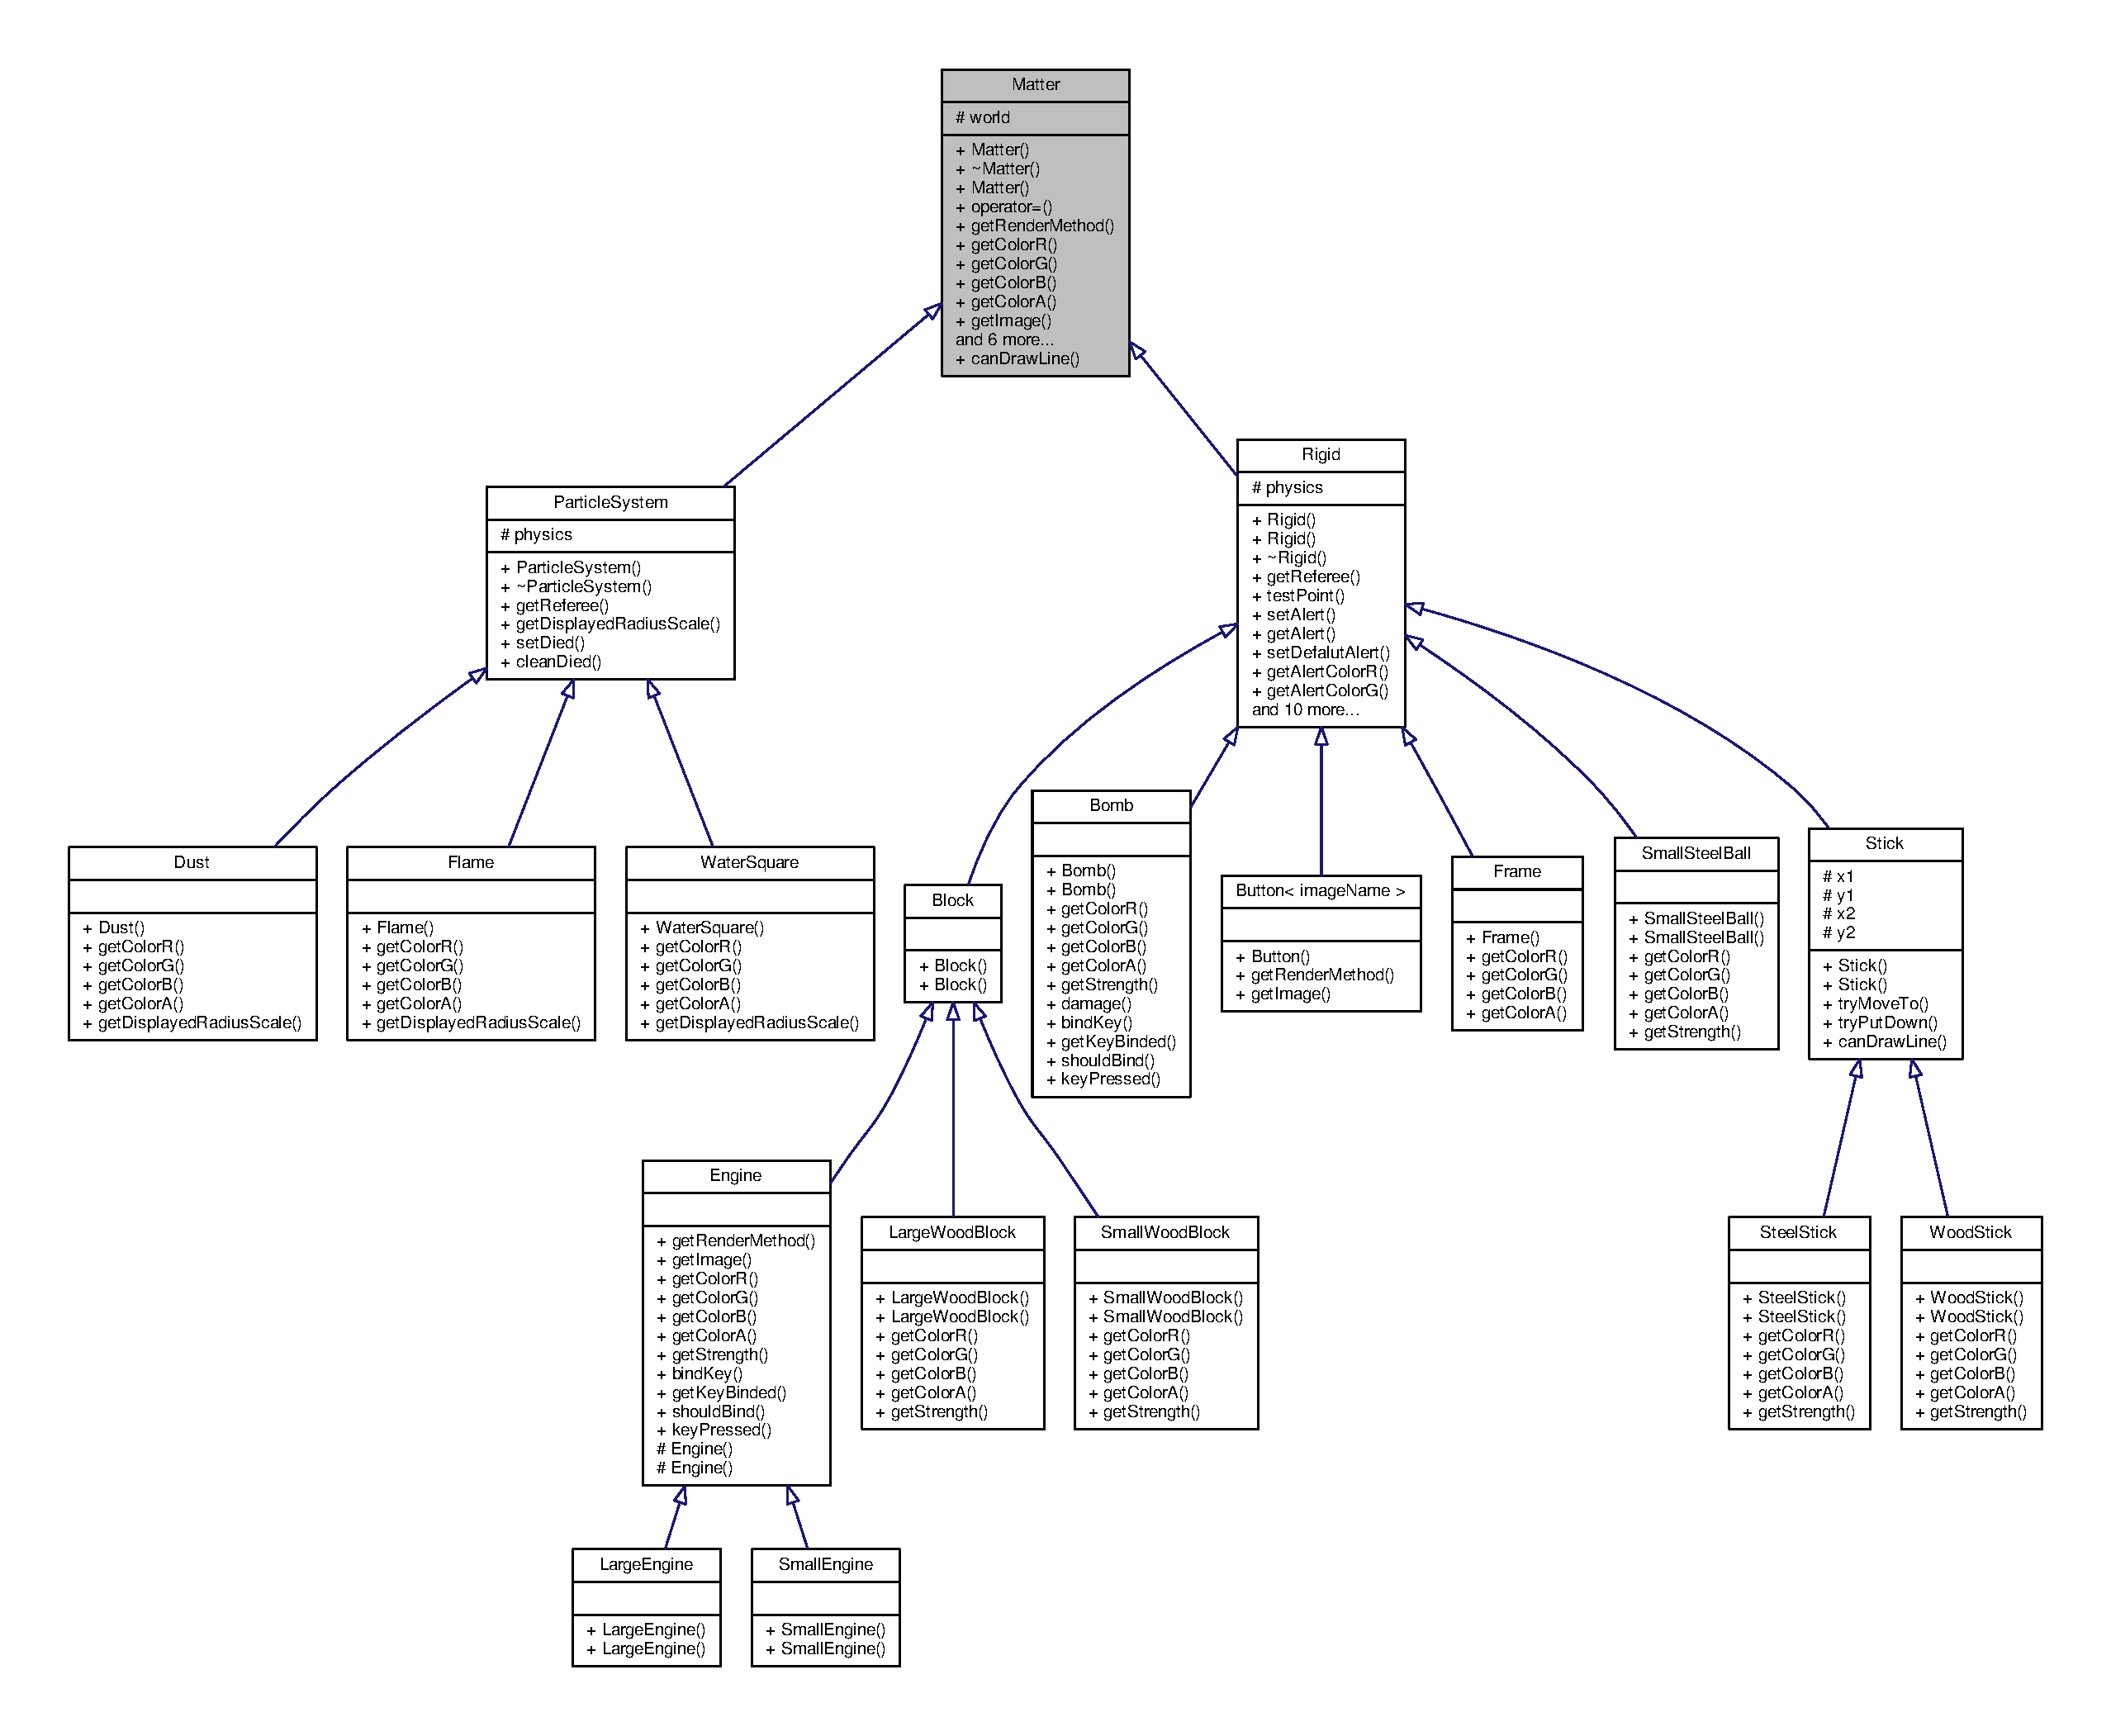
\includegraphics[width=350pt]{classMatter__inherit__graph}
\end{center}
\end{figure}


Collaboration diagram for Matter\+:
\nopagebreak
\begin{figure}[H]
\begin{center}
\leavevmode
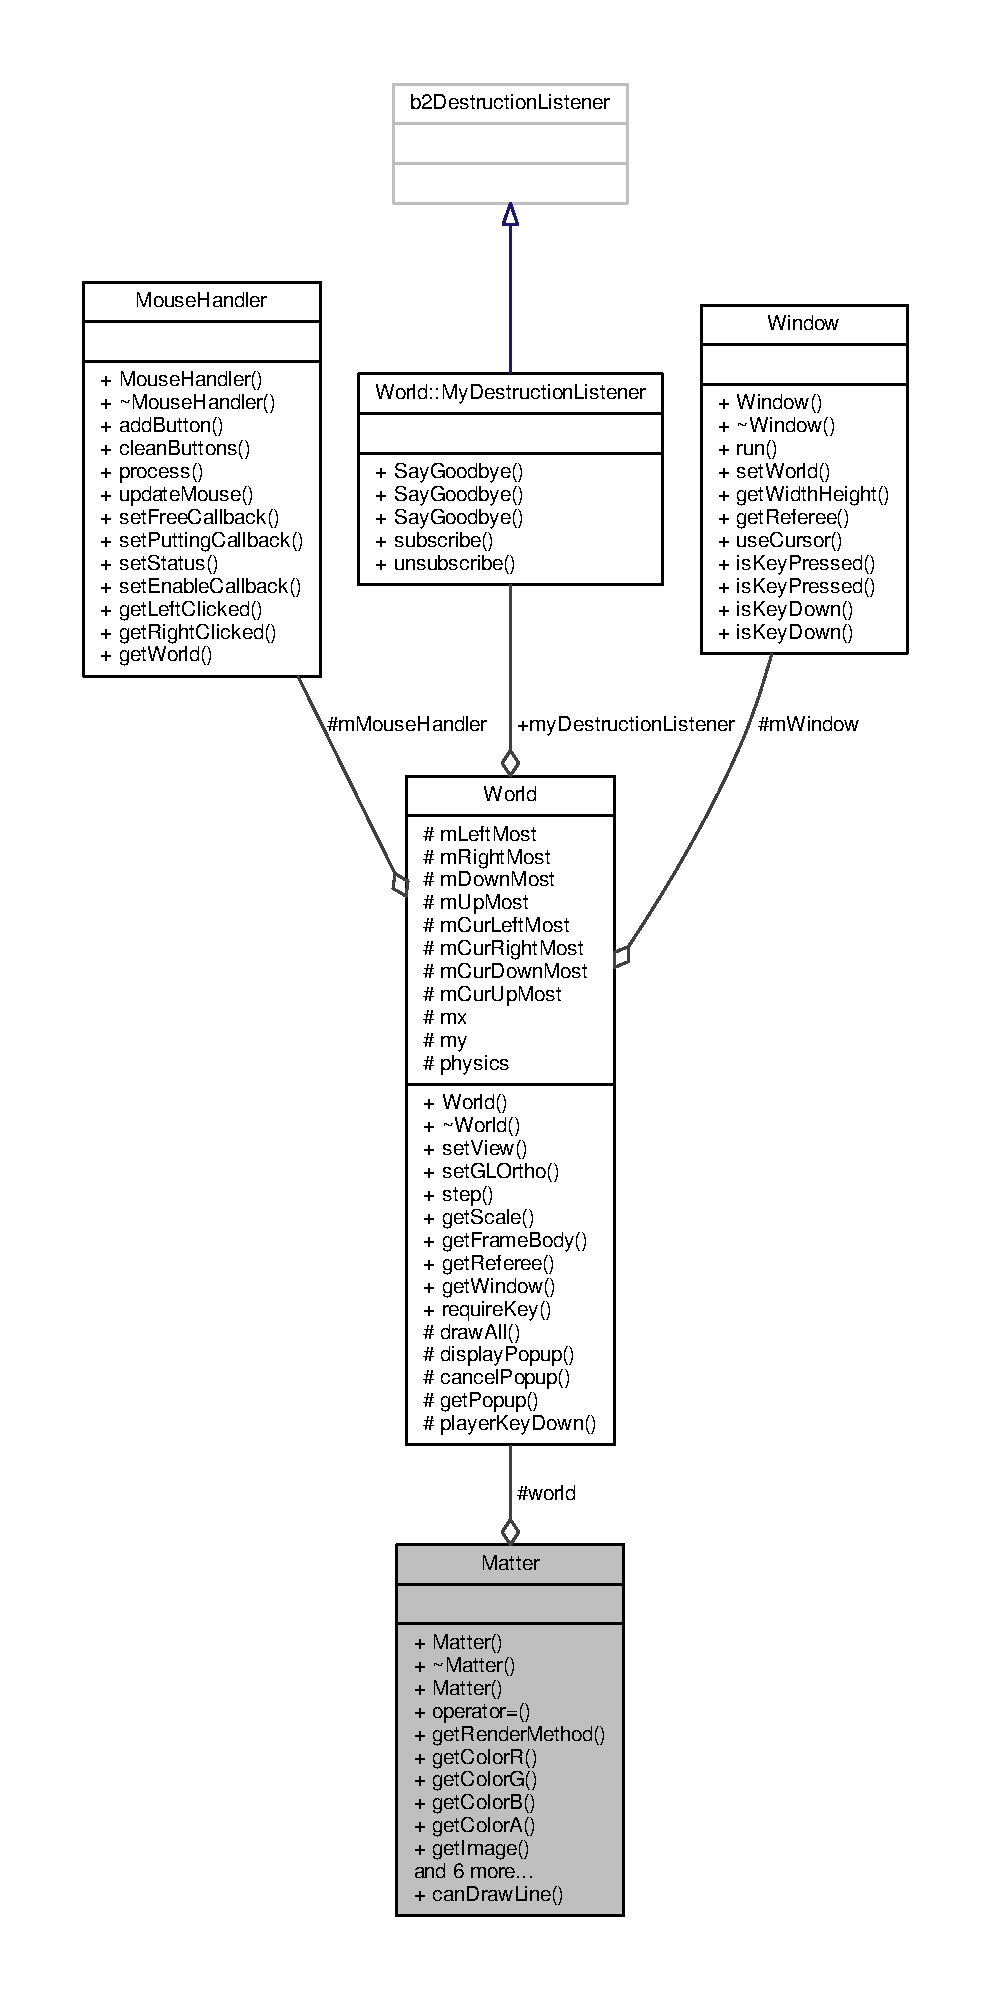
\includegraphics[height=550pt]{classMatter__coll__graph}
\end{center}
\end{figure}
\subsection*{Public Types}
\begin{DoxyCompactItemize}
\item 
enum \hyperlink{classMatter_ade1ce1bf81f25377f689d103cd431907}{Render\+Method} \{ \hyperlink{classMatter_ade1ce1bf81f25377f689d103cd431907ad7201b31cb7302539e30e60b05464bae}{R\+E\+N\+D\+E\+R\+\_\+\+C\+O\+L\+O\+R} = 0, 
\hyperlink{classMatter_ade1ce1bf81f25377f689d103cd431907a0a15cf1b6cb2aa933e52d880a175c932}{R\+E\+N\+D\+E\+R\+\_\+\+T\+E\+X\+T\+U\+R\+E} = 1, 
\hyperlink{classMatter_ade1ce1bf81f25377f689d103cd431907ae26bb08225540fe1771201e859e04021}{R\+E\+N\+D\+E\+R\+\_\+\+C\+O\+L\+O\+R\+\_\+\+W\+I\+T\+H\+\_\+\+T\+E\+X\+T\+U\+R\+E} = 2
 \}
\end{DoxyCompactItemize}
\subsection*{Public Member Functions}
\begin{DoxyCompactItemize}
\item 
\hyperlink{classMatter_a7553dd6bd2e7863c2fd59c388916a87b}{Matter} (\hyperlink{classWorld}{World} $\ast$\+\_\+world) noexcept
\item 
virtual \hyperlink{classMatter_a2087311945c6e5fe470bf404f85e4bde}{$\sim$\+Matter} () noexcept
\item 
\hyperlink{classMatter_ae3afe6f6b9571ee1e2fe401a90d5c407}{Matter} (const \hyperlink{classMatter}{Matter} \&)=delete
\item 
\hyperlink{classMatter}{Matter} \& \hyperlink{classMatter_a3e44ded88dc43c882843ccaf6ceaeda0}{operator=} (const \hyperlink{classMatter}{Matter} \&)=delete
\item 
virtual \hyperlink{classMatter_ade1ce1bf81f25377f689d103cd431907}{Render\+Method} \hyperlink{classMatter_a3d6823a375fe0a537837b905b44af5bd}{get\+Render\+Method} () const 
\item 
virtual float \hyperlink{classMatter_a926d246584228c3e3b102dbfd42036ec}{get\+Color\+R} () const 
\item 
virtual float \hyperlink{classMatter_aa3fcdc82f788fbf873ec3ff4808f614a}{get\+Color\+G} () const 
\item 
virtual float \hyperlink{classMatter_af830da17da427c84c7f6deee4a91b3d4}{get\+Color\+B} () const 
\item 
virtual float \hyperlink{classMatter_aa44ee7ba48cb9a582a6f86e1e9e2ef38}{get\+Color\+A} () const 
\item 
virtual \hyperlink{image_8h_af9361b398b5cfcafbe93f82e8eaeb080}{Image\+Name} \hyperlink{classMatter_ad6202a62e4ae27dde457c56520f1865e}{get\+Image} () const 
\item 
void \hyperlink{classMatter_a678834a886a610754ea863751fb6c046}{set\+Depth} (float \+\_\+depth)
\item 
float \hyperlink{classMatter_aa0f6ed46b01aac5f7404635cbba56c3e}{get\+Depth} () const 
\item 
void \hyperlink{classMatter_a3e7f9e8ade54d7c5fbb82da57f5b0ff8}{set\+Player} (int \+\_\+player)
\begin{DoxyCompactList}\small\item\em player = -\/1 \+: user, 0 \+: none, $>$0 \+: enemy \end{DoxyCompactList}\item 
int \hyperlink{classMatter_a5942bf485f1c095b0abd79ea13239cc7}{get\+Player} () const 
\item 
void \hyperlink{classMatter_a72a6f33a55d6df477dc8e684924bee55}{set\+Is\+User\+Created} (bool \hyperlink{image_8h_ab2d05693952610f937e5acb3c4a8fa1b}{b})
\begin{DoxyCompactList}\small\item\em mark to be created by users \end{DoxyCompactList}\item 
bool \hyperlink{classMatter_ac46cc6630fca6195dc0cd455505a8d84}{get\+Is\+User\+Created} () const 
\begin{DoxyCompactList}\small\item\em determine whether it is created by users \end{DoxyCompactList}\end{DoxyCompactItemize}
\subsection*{Static Public Member Functions}
\begin{DoxyCompactItemize}
\item 
static bool \hyperlink{classMatter_afe85d0688495f35bfe2cf4443c5fc34f}{can\+Draw\+Line} ()
\begin{DoxyCompactList}\small\item\em Specify whether user can create objects by drawing lines Can be overidden. \end{DoxyCompactList}\end{DoxyCompactItemize}
\subsection*{Protected Attributes}
\begin{DoxyCompactItemize}
\item 
\hyperlink{classWorld}{World} $\ast$ \hyperlink{classMatter_abdc5b13e2427e41c45af024acae015f1}{world}
\end{DoxyCompactItemize}
\subsection*{Private Attributes}
\begin{DoxyCompactItemize}
\item 
float \hyperlink{classMatter_ae6c374ad27e583eb3a675350914394ae}{depth}
\item 
int \hyperlink{classMatter_a702c712519468f6f68bc945f771c5044}{player}
\end{DoxyCompactItemize}


\subsection{Detailed Description}
Base class of all rigid bodies and particles. 

\subsection{Member Enumeration Documentation}
\hypertarget{classMatter_ade1ce1bf81f25377f689d103cd431907}{}\index{Matter@{Matter}!Render\+Method@{Render\+Method}}
\index{Render\+Method@{Render\+Method}!Matter@{Matter}}
\subsubsection[{Render\+Method}]{\setlength{\rightskip}{0pt plus 5cm}enum {\bf Matter\+::\+Render\+Method}}\label{classMatter_ade1ce1bf81f25377f689d103cd431907}
\begin{Desc}
\item[Enumerator]\par
\begin{description}
\index{R\+E\+N\+D\+E\+R\+\_\+\+C\+O\+L\+O\+R@{R\+E\+N\+D\+E\+R\+\_\+\+C\+O\+L\+O\+R}!Matter@{Matter}}\index{Matter@{Matter}!R\+E\+N\+D\+E\+R\+\_\+\+C\+O\+L\+O\+R@{R\+E\+N\+D\+E\+R\+\_\+\+C\+O\+L\+O\+R}}\item[{\em 
\hypertarget{classMatter_ade1ce1bf81f25377f689d103cd431907ad7201b31cb7302539e30e60b05464bae}{}R\+E\+N\+D\+E\+R\+\_\+\+C\+O\+L\+O\+R\label{classMatter_ade1ce1bf81f25377f689d103cd431907ad7201b31cb7302539e30e60b05464bae}
}]\index{R\+E\+N\+D\+E\+R\+\_\+\+T\+E\+X\+T\+U\+R\+E@{R\+E\+N\+D\+E\+R\+\_\+\+T\+E\+X\+T\+U\+R\+E}!Matter@{Matter}}\index{Matter@{Matter}!R\+E\+N\+D\+E\+R\+\_\+\+T\+E\+X\+T\+U\+R\+E@{R\+E\+N\+D\+E\+R\+\_\+\+T\+E\+X\+T\+U\+R\+E}}\item[{\em 
\hypertarget{classMatter_ade1ce1bf81f25377f689d103cd431907a0a15cf1b6cb2aa933e52d880a175c932}{}R\+E\+N\+D\+E\+R\+\_\+\+T\+E\+X\+T\+U\+R\+E\label{classMatter_ade1ce1bf81f25377f689d103cd431907a0a15cf1b6cb2aa933e52d880a175c932}
}]\index{R\+E\+N\+D\+E\+R\+\_\+\+C\+O\+L\+O\+R\+\_\+\+W\+I\+T\+H\+\_\+\+T\+E\+X\+T\+U\+R\+E@{R\+E\+N\+D\+E\+R\+\_\+\+C\+O\+L\+O\+R\+\_\+\+W\+I\+T\+H\+\_\+\+T\+E\+X\+T\+U\+R\+E}!Matter@{Matter}}\index{Matter@{Matter}!R\+E\+N\+D\+E\+R\+\_\+\+C\+O\+L\+O\+R\+\_\+\+W\+I\+T\+H\+\_\+\+T\+E\+X\+T\+U\+R\+E@{R\+E\+N\+D\+E\+R\+\_\+\+C\+O\+L\+O\+R\+\_\+\+W\+I\+T\+H\+\_\+\+T\+E\+X\+T\+U\+R\+E}}\item[{\em 
\hypertarget{classMatter_ade1ce1bf81f25377f689d103cd431907ae26bb08225540fe1771201e859e04021}{}R\+E\+N\+D\+E\+R\+\_\+\+C\+O\+L\+O\+R\+\_\+\+W\+I\+T\+H\+\_\+\+T\+E\+X\+T\+U\+R\+E\label{classMatter_ade1ce1bf81f25377f689d103cd431907ae26bb08225540fe1771201e859e04021}
}]\end{description}
\end{Desc}


\subsection{Constructor \& Destructor Documentation}
\hypertarget{classMatter_a7553dd6bd2e7863c2fd59c388916a87b}{}\index{Matter@{Matter}!Matter@{Matter}}
\index{Matter@{Matter}!Matter@{Matter}}
\subsubsection[{Matter}]{\setlength{\rightskip}{0pt plus 5cm}Matter\+::\+Matter (
\begin{DoxyParamCaption}
\item[{{\bf World} $\ast$}]{\+\_\+world}
\end{DoxyParamCaption}
)\hspace{0.3cm}{\ttfamily [inline]}, {\ttfamily [noexcept]}}\label{classMatter_a7553dd6bd2e7863c2fd59c388916a87b}
\hypertarget{classMatter_a2087311945c6e5fe470bf404f85e4bde}{}\index{Matter@{Matter}!````~Matter@{$\sim$\+Matter}}
\index{````~Matter@{$\sim$\+Matter}!Matter@{Matter}}
\subsubsection[{$\sim$\+Matter}]{\setlength{\rightskip}{0pt plus 5cm}virtual Matter\+::$\sim$\+Matter (
\begin{DoxyParamCaption}
{}
\end{DoxyParamCaption}
)\hspace{0.3cm}{\ttfamily [inline]}, {\ttfamily [virtual]}, {\ttfamily [noexcept]}}\label{classMatter_a2087311945c6e5fe470bf404f85e4bde}
\hypertarget{classMatter_ae3afe6f6b9571ee1e2fe401a90d5c407}{}\index{Matter@{Matter}!Matter@{Matter}}
\index{Matter@{Matter}!Matter@{Matter}}
\subsubsection[{Matter}]{\setlength{\rightskip}{0pt plus 5cm}Matter\+::\+Matter (
\begin{DoxyParamCaption}
\item[{const {\bf Matter} \&}]{}
\end{DoxyParamCaption}
)\hspace{0.3cm}{\ttfamily [delete]}}\label{classMatter_ae3afe6f6b9571ee1e2fe401a90d5c407}


\subsection{Member Function Documentation}
\hypertarget{classMatter_afe85d0688495f35bfe2cf4443c5fc34f}{}\index{Matter@{Matter}!can\+Draw\+Line@{can\+Draw\+Line}}
\index{can\+Draw\+Line@{can\+Draw\+Line}!Matter@{Matter}}
\subsubsection[{can\+Draw\+Line}]{\setlength{\rightskip}{0pt plus 5cm}static bool Matter\+::can\+Draw\+Line (
\begin{DoxyParamCaption}
{}
\end{DoxyParamCaption}
)\hspace{0.3cm}{\ttfamily [inline]}, {\ttfamily [static]}}\label{classMatter_afe85d0688495f35bfe2cf4443c5fc34f}


Specify whether user can create objects by drawing lines Can be overidden. 

\hypertarget{classMatter_aa44ee7ba48cb9a582a6f86e1e9e2ef38}{}\index{Matter@{Matter}!get\+Color\+A@{get\+Color\+A}}
\index{get\+Color\+A@{get\+Color\+A}!Matter@{Matter}}
\subsubsection[{get\+Color\+A}]{\setlength{\rightskip}{0pt plus 5cm}virtual float Matter\+::get\+Color\+A (
\begin{DoxyParamCaption}
{}
\end{DoxyParamCaption}
) const\hspace{0.3cm}{\ttfamily [inline]}, {\ttfamily [virtual]}}\label{classMatter_aa44ee7ba48cb9a582a6f86e1e9e2ef38}


Reimplemented in \hyperlink{classFlame_a9730bb5ff22bdf2ab579eb9ae1d8a37f}{Flame}, \hyperlink{classDust_a6a61ed84ae1cbba8d0cdbc102a343f0f}{Dust}, \hyperlink{classWaterSquare_a7f549f3b3c9b7a350aa2ae62c4db7ce5}{Water\+Square}, \hyperlink{classWoodStick_a4fd46786dec67fff538e6b6c1df6fe47}{Wood\+Stick}, \hyperlink{classSteelStick_ac4d726f343aa8cd6c2d3306855ba48c2}{Steel\+Stick}, \hyperlink{classFrame_a99769eacd74a31fc9d198f83bc6616db}{Frame}, \hyperlink{classBomb_a19e85b4632b547de51bde57844065efa}{Bomb}, \hyperlink{classSmallSteelBall_a2d11278708166ac6b05165baf86c1046}{Small\+Steel\+Ball}, \hyperlink{classEngine_aefe56a242ce462d18958c2e217a0df7a}{Engine}, \hyperlink{classLargeWoodBlock_a74390f6c417c547b18db713696d2a12d}{Large\+Wood\+Block}, and \hyperlink{classSmallWoodBlock_a88c753e9e05364d2a872250bed48563d}{Small\+Wood\+Block}.

\hypertarget{classMatter_af830da17da427c84c7f6deee4a91b3d4}{}\index{Matter@{Matter}!get\+Color\+B@{get\+Color\+B}}
\index{get\+Color\+B@{get\+Color\+B}!Matter@{Matter}}
\subsubsection[{get\+Color\+B}]{\setlength{\rightskip}{0pt plus 5cm}virtual float Matter\+::get\+Color\+B (
\begin{DoxyParamCaption}
{}
\end{DoxyParamCaption}
) const\hspace{0.3cm}{\ttfamily [inline]}, {\ttfamily [virtual]}}\label{classMatter_af830da17da427c84c7f6deee4a91b3d4}


Reimplemented in \hyperlink{classFlame_abbd9b48e0a3744f4a9c59df52e8c8ca1}{Flame}, \hyperlink{classDust_a088431d5f6a114d93f12cae63592a8dd}{Dust}, \hyperlink{classWaterSquare_a6dd404113fa8377a06d4dd62fd711578}{Water\+Square}, \hyperlink{classWoodStick_a2483dcaaadabd32b1a23789727b777fe}{Wood\+Stick}, \hyperlink{classSteelStick_aa766a601b7b048d7afbe593d7a1b544d}{Steel\+Stick}, \hyperlink{classFrame_aac730f8f9ae5f59cb6a1814d56a8eefa}{Frame}, \hyperlink{classBomb_a31ede414b7c9c3ef82ea201975d7fd25}{Bomb}, \hyperlink{classSmallSteelBall_a7ebf920ae4d29ca94edc7ad390031c37}{Small\+Steel\+Ball}, \hyperlink{classEngine_aefc235452646da3c6b9b77c625ef3278}{Engine}, \hyperlink{classLargeWoodBlock_ac2499af4b661efeeee7662dff8af48f2}{Large\+Wood\+Block}, and \hyperlink{classSmallWoodBlock_ad85ea47531644ea51905b2fbe014122d}{Small\+Wood\+Block}.

\hypertarget{classMatter_aa3fcdc82f788fbf873ec3ff4808f614a}{}\index{Matter@{Matter}!get\+Color\+G@{get\+Color\+G}}
\index{get\+Color\+G@{get\+Color\+G}!Matter@{Matter}}
\subsubsection[{get\+Color\+G}]{\setlength{\rightskip}{0pt plus 5cm}virtual float Matter\+::get\+Color\+G (
\begin{DoxyParamCaption}
{}
\end{DoxyParamCaption}
) const\hspace{0.3cm}{\ttfamily [inline]}, {\ttfamily [virtual]}}\label{classMatter_aa3fcdc82f788fbf873ec3ff4808f614a}


Reimplemented in \hyperlink{classFlame_a52151a48e25d77440ea47b3479501d36}{Flame}, \hyperlink{classDust_a386313dcd344747fb28bb809f6243bf8}{Dust}, \hyperlink{classWaterSquare_ae63df10dd32846cca279aef4f86da099}{Water\+Square}, \hyperlink{classWoodStick_a97395092b892cab30d590cb87177bcac}{Wood\+Stick}, \hyperlink{classSteelStick_a3af94ded9f36368b79a5913de3ecef3a}{Steel\+Stick}, \hyperlink{classFrame_a44139c9e8bee6504c43bb6bc21b1d599}{Frame}, \hyperlink{classBomb_a393fa1faa9cfdadb0d0202983de6e16b}{Bomb}, \hyperlink{classSmallSteelBall_a8d15df33cfeb00bd61060c7197250989}{Small\+Steel\+Ball}, \hyperlink{classEngine_abd2e81839210c4c98b6cad705af25cec}{Engine}, \hyperlink{classLargeWoodBlock_ae422ccf33effdf80ee4bf7688de05b92}{Large\+Wood\+Block}, and \hyperlink{classSmallWoodBlock_ac83d1610c7a0acf7ac8a1eb569b92380}{Small\+Wood\+Block}.

\hypertarget{classMatter_a926d246584228c3e3b102dbfd42036ec}{}\index{Matter@{Matter}!get\+Color\+R@{get\+Color\+R}}
\index{get\+Color\+R@{get\+Color\+R}!Matter@{Matter}}
\subsubsection[{get\+Color\+R}]{\setlength{\rightskip}{0pt plus 5cm}virtual float Matter\+::get\+Color\+R (
\begin{DoxyParamCaption}
{}
\end{DoxyParamCaption}
) const\hspace{0.3cm}{\ttfamily [inline]}, {\ttfamily [virtual]}}\label{classMatter_a926d246584228c3e3b102dbfd42036ec}


Reimplemented in \hyperlink{classFlame_a3cdb607d9cadaeb164494ea2334c4bf8}{Flame}, \hyperlink{classDust_a2e5d596ac110553eb401eae59641fb5a}{Dust}, \hyperlink{classWaterSquare_ae34b29db832bbe03ce6521493a17fac3}{Water\+Square}, \hyperlink{classWoodStick_a7c22e5a82627ab9a90fcd0236eacb4bc}{Wood\+Stick}, \hyperlink{classSteelStick_aaa82c2460e492c249074058a83245634}{Steel\+Stick}, \hyperlink{classFrame_a1f5aa3b4dd7b90959a95c1e54f01a1e4}{Frame}, \hyperlink{classBomb_aa95b13c06660f7eaee26dbb75cda41ed}{Bomb}, \hyperlink{classSmallSteelBall_aa15f3c1c1a2596edecb048b8a32f5d55}{Small\+Steel\+Ball}, \hyperlink{classEngine_a9ad7ea816b850dc812b6a792493a803e}{Engine}, \hyperlink{classLargeWoodBlock_a3eeebdbf61b9f33a02b5c845f31ba428}{Large\+Wood\+Block}, and \hyperlink{classSmallWoodBlock_a8cb7ec9e82df6465c1d069e1d3167d4c}{Small\+Wood\+Block}.

\hypertarget{classMatter_aa0f6ed46b01aac5f7404635cbba56c3e}{}\index{Matter@{Matter}!get\+Depth@{get\+Depth}}
\index{get\+Depth@{get\+Depth}!Matter@{Matter}}
\subsubsection[{get\+Depth}]{\setlength{\rightskip}{0pt plus 5cm}float Matter\+::get\+Depth (
\begin{DoxyParamCaption}
{}
\end{DoxyParamCaption}
) const\hspace{0.3cm}{\ttfamily [inline]}}\label{classMatter_aa0f6ed46b01aac5f7404635cbba56c3e}
\hypertarget{classMatter_ad6202a62e4ae27dde457c56520f1865e}{}\index{Matter@{Matter}!get\+Image@{get\+Image}}
\index{get\+Image@{get\+Image}!Matter@{Matter}}
\subsubsection[{get\+Image}]{\setlength{\rightskip}{0pt plus 5cm}virtual {\bf Image\+Name} Matter\+::get\+Image (
\begin{DoxyParamCaption}
{}
\end{DoxyParamCaption}
) const\hspace{0.3cm}{\ttfamily [inline]}, {\ttfamily [virtual]}}\label{classMatter_ad6202a62e4ae27dde457c56520f1865e}


Reimplemented in \hyperlink{classButton_a75331f4a815ee394a223812681460e09}{Button$<$ image\+Name $>$}, and \hyperlink{classEngine_a130b5e67a05c2ea6f9c2f5d7a4fc60dd}{Engine}.

\hypertarget{classMatter_ac46cc6630fca6195dc0cd455505a8d84}{}\index{Matter@{Matter}!get\+Is\+User\+Created@{get\+Is\+User\+Created}}
\index{get\+Is\+User\+Created@{get\+Is\+User\+Created}!Matter@{Matter}}
\subsubsection[{get\+Is\+User\+Created}]{\setlength{\rightskip}{0pt plus 5cm}bool Matter\+::get\+Is\+User\+Created (
\begin{DoxyParamCaption}
{}
\end{DoxyParamCaption}
) const\hspace{0.3cm}{\ttfamily [inline]}}\label{classMatter_ac46cc6630fca6195dc0cd455505a8d84}


determine whether it is created by users 

\hypertarget{classMatter_a5942bf485f1c095b0abd79ea13239cc7}{}\index{Matter@{Matter}!get\+Player@{get\+Player}}
\index{get\+Player@{get\+Player}!Matter@{Matter}}
\subsubsection[{get\+Player}]{\setlength{\rightskip}{0pt plus 5cm}int Matter\+::get\+Player (
\begin{DoxyParamCaption}
{}
\end{DoxyParamCaption}
) const\hspace{0.3cm}{\ttfamily [inline]}}\label{classMatter_a5942bf485f1c095b0abd79ea13239cc7}
\hypertarget{classMatter_a3d6823a375fe0a537837b905b44af5bd}{}\index{Matter@{Matter}!get\+Render\+Method@{get\+Render\+Method}}
\index{get\+Render\+Method@{get\+Render\+Method}!Matter@{Matter}}
\subsubsection[{get\+Render\+Method}]{\setlength{\rightskip}{0pt plus 5cm}virtual {\bf Render\+Method} Matter\+::get\+Render\+Method (
\begin{DoxyParamCaption}
{}
\end{DoxyParamCaption}
) const\hspace{0.3cm}{\ttfamily [inline]}, {\ttfamily [virtual]}}\label{classMatter_a3d6823a375fe0a537837b905b44af5bd}


Reimplemented in \hyperlink{classButton_a50233f0c531652154ecc0f8f7dc26571}{Button$<$ image\+Name $>$}, and \hyperlink{classEngine_a72c7a3ea05ac92bdb909e11b20d8d6fc}{Engine}.

\hypertarget{classMatter_a3e44ded88dc43c882843ccaf6ceaeda0}{}\index{Matter@{Matter}!operator=@{operator=}}
\index{operator=@{operator=}!Matter@{Matter}}
\subsubsection[{operator=}]{\setlength{\rightskip}{0pt plus 5cm}{\bf Matter}\& Matter\+::operator= (
\begin{DoxyParamCaption}
\item[{const {\bf Matter} \&}]{}
\end{DoxyParamCaption}
)\hspace{0.3cm}{\ttfamily [delete]}}\label{classMatter_a3e44ded88dc43c882843ccaf6ceaeda0}
\hypertarget{classMatter_a678834a886a610754ea863751fb6c046}{}\index{Matter@{Matter}!set\+Depth@{set\+Depth}}
\index{set\+Depth@{set\+Depth}!Matter@{Matter}}
\subsubsection[{set\+Depth}]{\setlength{\rightskip}{0pt plus 5cm}void Matter\+::set\+Depth (
\begin{DoxyParamCaption}
\item[{float}]{\+\_\+depth}
\end{DoxyParamCaption}
)\hspace{0.3cm}{\ttfamily [inline]}}\label{classMatter_a678834a886a610754ea863751fb6c046}
\hypertarget{classMatter_a72a6f33a55d6df477dc8e684924bee55}{}\index{Matter@{Matter}!set\+Is\+User\+Created@{set\+Is\+User\+Created}}
\index{set\+Is\+User\+Created@{set\+Is\+User\+Created}!Matter@{Matter}}
\subsubsection[{set\+Is\+User\+Created}]{\setlength{\rightskip}{0pt plus 5cm}void Matter\+::set\+Is\+User\+Created (
\begin{DoxyParamCaption}
\item[{bool}]{b}
\end{DoxyParamCaption}
)\hspace{0.3cm}{\ttfamily [inline]}}\label{classMatter_a72a6f33a55d6df477dc8e684924bee55}


mark to be created by users 

\hypertarget{classMatter_a3e7f9e8ade54d7c5fbb82da57f5b0ff8}{}\index{Matter@{Matter}!set\+Player@{set\+Player}}
\index{set\+Player@{set\+Player}!Matter@{Matter}}
\subsubsection[{set\+Player}]{\setlength{\rightskip}{0pt plus 5cm}void Matter\+::set\+Player (
\begin{DoxyParamCaption}
\item[{int}]{\+\_\+player}
\end{DoxyParamCaption}
)\hspace{0.3cm}{\ttfamily [inline]}}\label{classMatter_a3e7f9e8ade54d7c5fbb82da57f5b0ff8}


player = -\/1 \+: user, 0 \+: none, $>$0 \+: enemy 



\subsection{Member Data Documentation}
\hypertarget{classMatter_ae6c374ad27e583eb3a675350914394ae}{}\index{Matter@{Matter}!depth@{depth}}
\index{depth@{depth}!Matter@{Matter}}
\subsubsection[{depth}]{\setlength{\rightskip}{0pt plus 5cm}float Matter\+::depth\hspace{0.3cm}{\ttfamily [private]}}\label{classMatter_ae6c374ad27e583eb3a675350914394ae}
\hypertarget{classMatter_a702c712519468f6f68bc945f771c5044}{}\index{Matter@{Matter}!player@{player}}
\index{player@{player}!Matter@{Matter}}
\subsubsection[{player}]{\setlength{\rightskip}{0pt plus 5cm}int Matter\+::player\hspace{0.3cm}{\ttfamily [private]}}\label{classMatter_a702c712519468f6f68bc945f771c5044}
\hypertarget{classMatter_abdc5b13e2427e41c45af024acae015f1}{}\index{Matter@{Matter}!world@{world}}
\index{world@{world}!Matter@{Matter}}
\subsubsection[{world}]{\setlength{\rightskip}{0pt plus 5cm}{\bf World}$\ast$ Matter\+::world\hspace{0.3cm}{\ttfamily [protected]}}\label{classMatter_abdc5b13e2427e41c45af024acae015f1}


The documentation for this class was generated from the following file\+:\begin{DoxyCompactItemize}
\item 
\hyperlink{matter_8h}{matter.\+h}\end{DoxyCompactItemize}

\hypertarget{classMouseCallback}{}\section{Mouse\+Callback Class Reference}
\label{classMouseCallback}\index{Mouse\+Callback@{Mouse\+Callback}}


This file consists of template classes of mouse callback listeners.  




{\ttfamily \#include $<$mousecallback.\+h$>$}



Inheritance diagram for Mouse\+Callback\+:\nopagebreak
\begin{figure}[H]
\begin{center}
\leavevmode
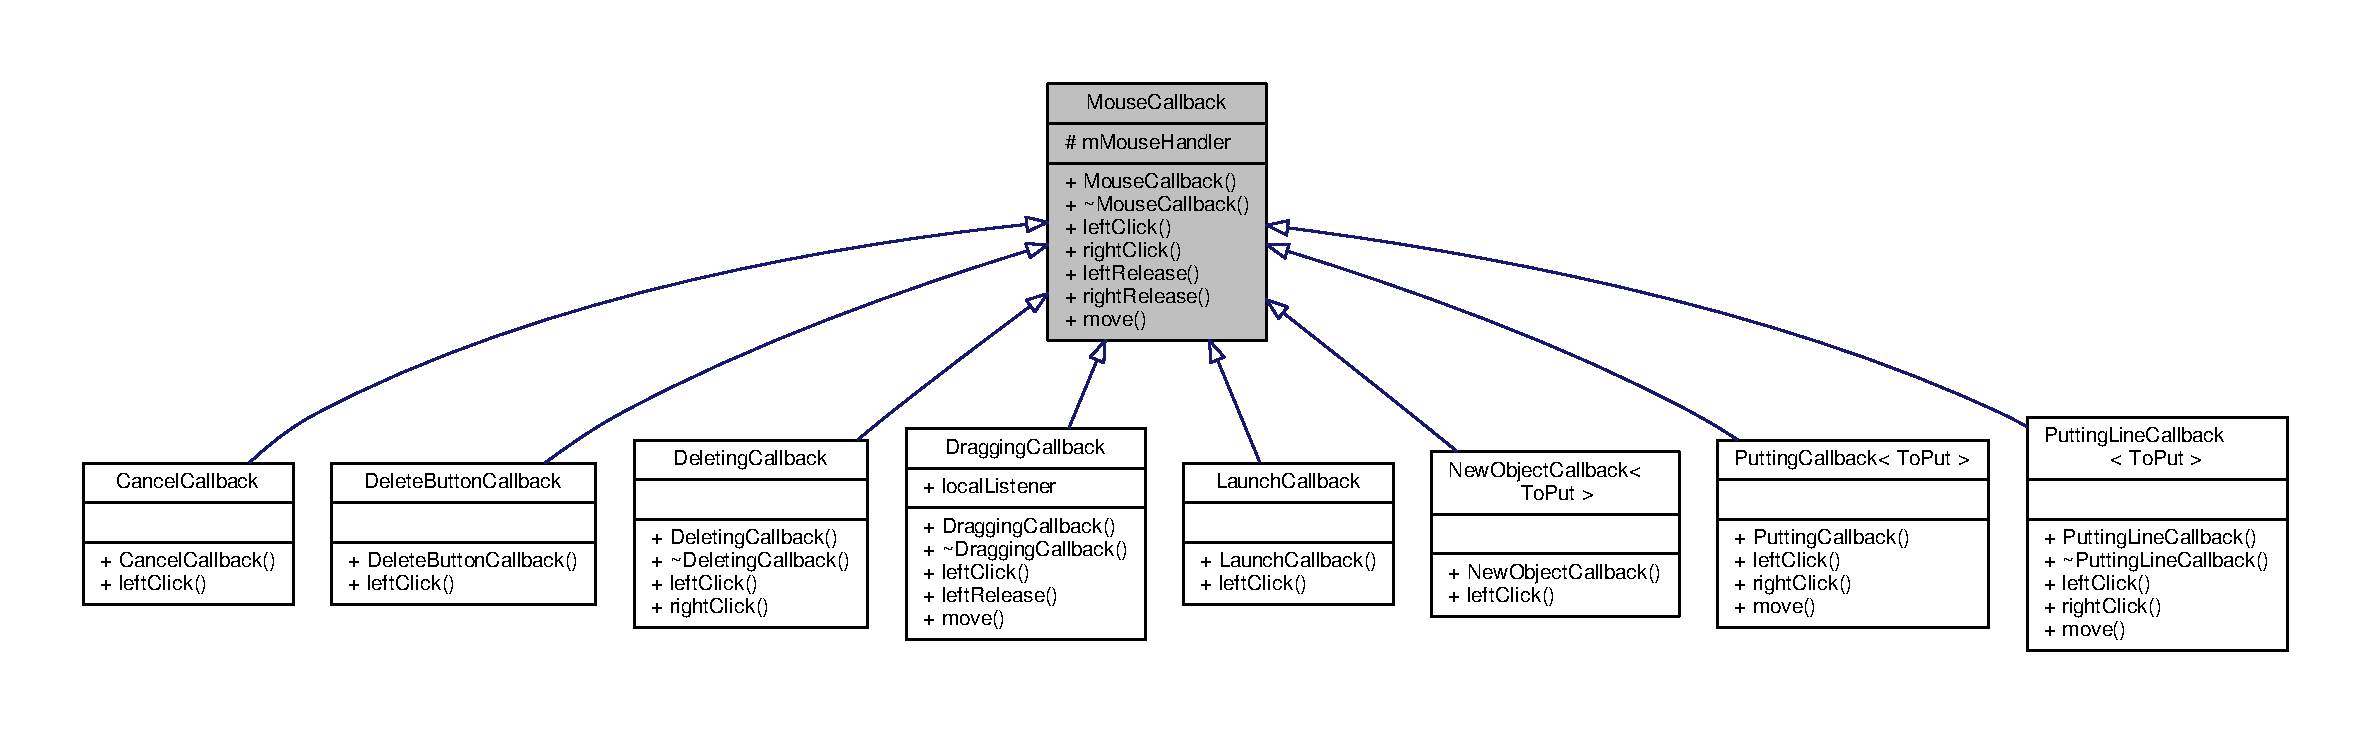
\includegraphics[width=350pt]{classMouseCallback__inherit__graph}
\end{center}
\end{figure}


Collaboration diagram for Mouse\+Callback\+:\nopagebreak
\begin{figure}[H]
\begin{center}
\leavevmode
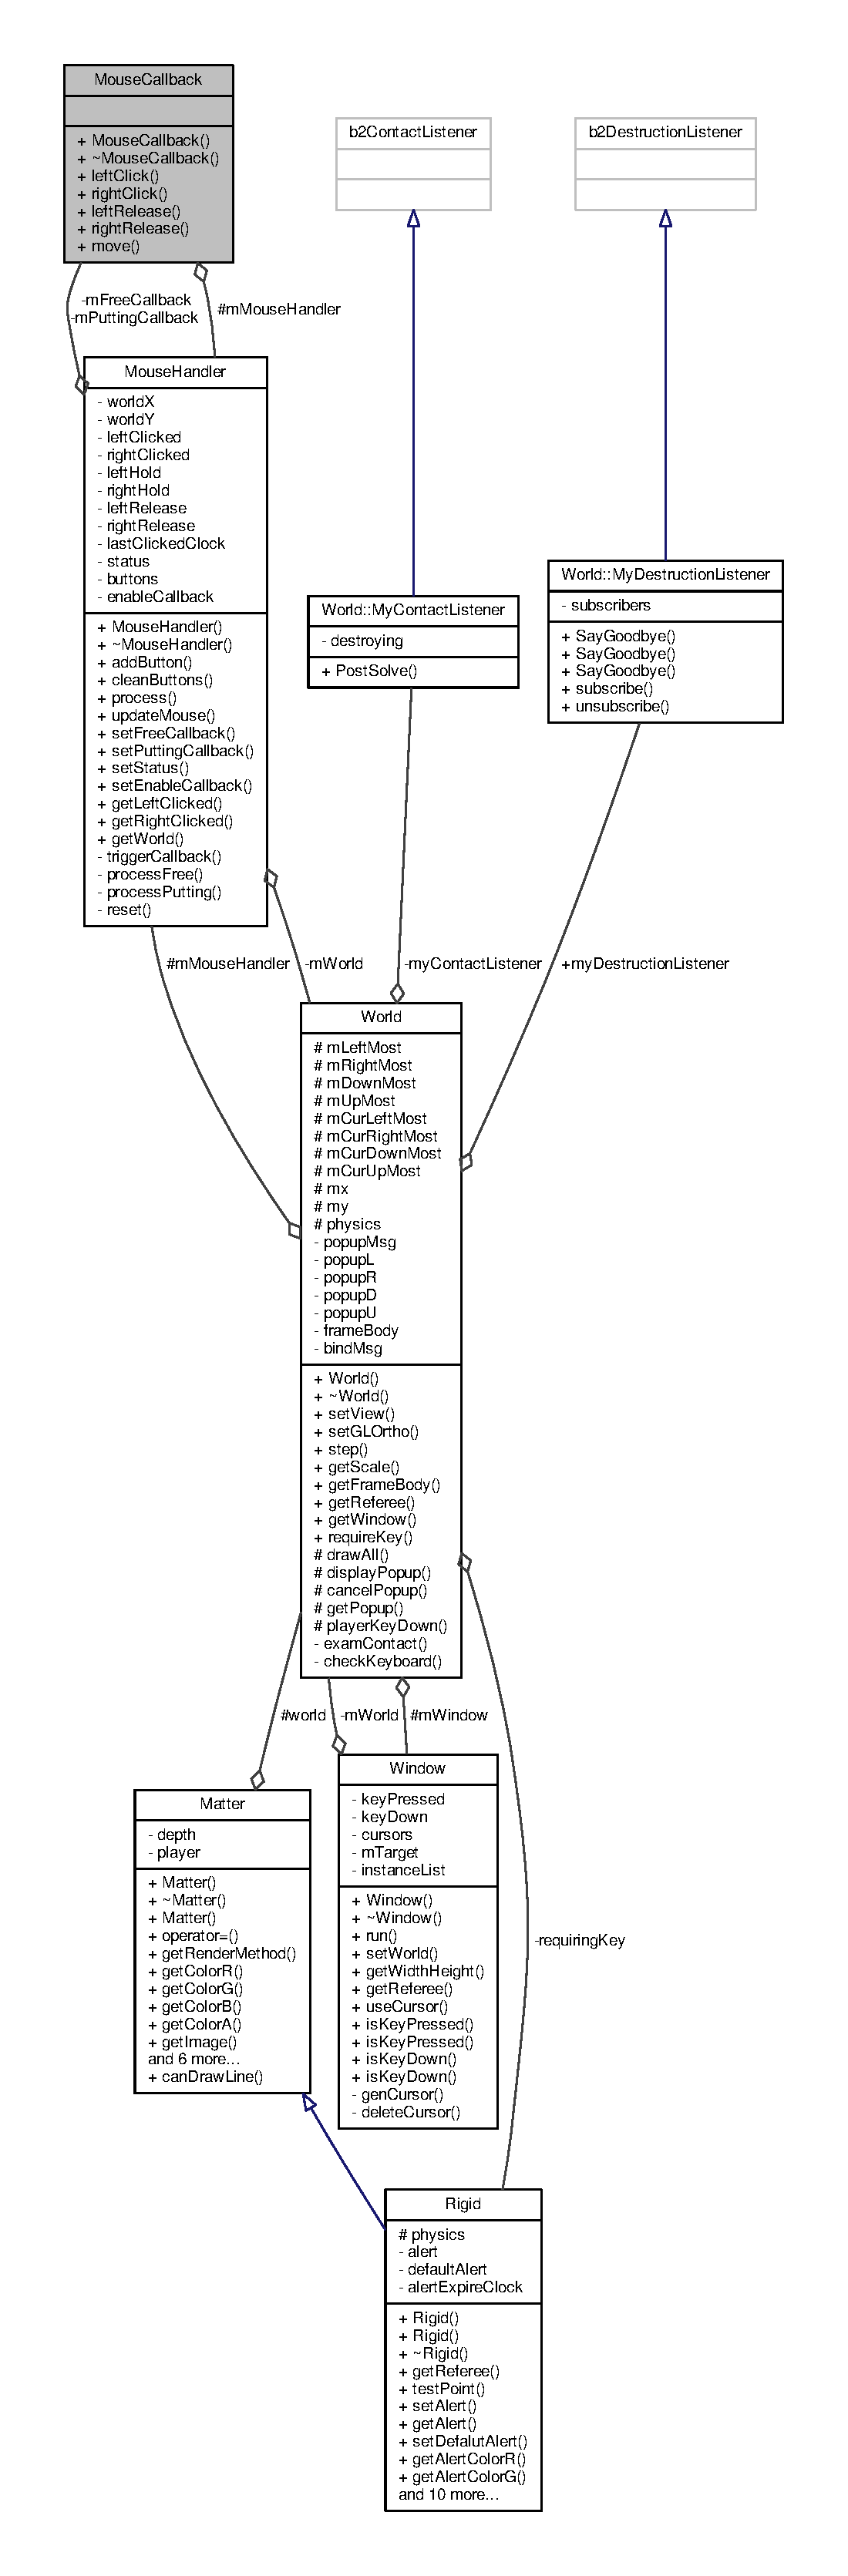
\includegraphics[width=217pt]{classMouseCallback__coll__graph}
\end{center}
\end{figure}
\subsection*{Public Member Functions}
\begin{DoxyCompactItemize}
\item 
\hyperlink{classMouseCallback_a0c6cd1db4b3bce0802f12256c6d7bf50}{Mouse\+Callback} (\hyperlink{classMouseHandler}{Mouse\+Handler} $\ast$\+\_\+handler)
\item 
virtual \hyperlink{classMouseCallback_a98466ace1354c848bd341b6baf5c92b5}{$\sim$\+Mouse\+Callback} ()
\item 
virtual void \hyperlink{classMouseCallback_a5ae88358471f1b48e3f6a730aaf0ba13}{left\+Click} (float x, float y)
\item 
virtual void \hyperlink{classMouseCallback_aa4a0c30b50b48972d0a48b9aff6344c5}{right\+Click} (float x, float y)
\item 
virtual void \hyperlink{classMouseCallback_a2a57b20538c6c7bf4a590140852bdd24}{left\+Release} (float x, float y)
\item 
virtual void \hyperlink{classMouseCallback_ab308a03d06ee903955875b36e1f31565}{right\+Release} (float x, float y)
\item 
virtual void \hyperlink{classMouseCallback_a9a667f1501597e44af0e0d9f1dfcbd6a}{move} (float x, float y)
\end{DoxyCompactItemize}
\subsection*{Protected Attributes}
\begin{DoxyCompactItemize}
\item 
\hyperlink{classMouseHandler}{Mouse\+Handler} $\ast$ \hyperlink{classMouseCallback_a6977cef81442eaa57f63d1995b31a240}{m\+Mouse\+Handler}
\end{DoxyCompactItemize}


\subsection{Detailed Description}
This file consists of template classes of mouse callback listeners. 

Handle according to mouse behaviors left\+Click and right\+Click will be triggered only once in a time interval. When mouse button actually released, left\+Release or right\+Release will be triggered. move will be triggered when all above are not triggerd. 

\subsection{Constructor \& Destructor Documentation}
\hypertarget{classMouseCallback_a0c6cd1db4b3bce0802f12256c6d7bf50}{}\index{Mouse\+Callback@{Mouse\+Callback}!Mouse\+Callback@{Mouse\+Callback}}
\index{Mouse\+Callback@{Mouse\+Callback}!Mouse\+Callback@{Mouse\+Callback}}
\subsubsection[{Mouse\+Callback}]{\setlength{\rightskip}{0pt plus 5cm}Mouse\+Callback\+::\+Mouse\+Callback (
\begin{DoxyParamCaption}
\item[{{\bf Mouse\+Handler} $\ast$}]{\+\_\+handler}
\end{DoxyParamCaption}
)\hspace{0.3cm}{\ttfamily [inline]}}\label{classMouseCallback_a0c6cd1db4b3bce0802f12256c6d7bf50}
\hypertarget{classMouseCallback_a98466ace1354c848bd341b6baf5c92b5}{}\index{Mouse\+Callback@{Mouse\+Callback}!````~Mouse\+Callback@{$\sim$\+Mouse\+Callback}}
\index{````~Mouse\+Callback@{$\sim$\+Mouse\+Callback}!Mouse\+Callback@{Mouse\+Callback}}
\subsubsection[{$\sim$\+Mouse\+Callback}]{\setlength{\rightskip}{0pt plus 5cm}virtual Mouse\+Callback\+::$\sim$\+Mouse\+Callback (
\begin{DoxyParamCaption}
{}
\end{DoxyParamCaption}
)\hspace{0.3cm}{\ttfamily [inline]}, {\ttfamily [virtual]}}\label{classMouseCallback_a98466ace1354c848bd341b6baf5c92b5}


\subsection{Member Function Documentation}
\hypertarget{classMouseCallback_a5ae88358471f1b48e3f6a730aaf0ba13}{}\index{Mouse\+Callback@{Mouse\+Callback}!left\+Click@{left\+Click}}
\index{left\+Click@{left\+Click}!Mouse\+Callback@{Mouse\+Callback}}
\subsubsection[{left\+Click}]{\setlength{\rightskip}{0pt plus 5cm}virtual void Mouse\+Callback\+::left\+Click (
\begin{DoxyParamCaption}
\item[{float}]{x, }
\item[{float}]{y}
\end{DoxyParamCaption}
)\hspace{0.3cm}{\ttfamily [inline]}, {\ttfamily [virtual]}}\label{classMouseCallback_a5ae88358471f1b48e3f6a730aaf0ba13}


Reimplemented in \hyperlink{classDraggingCallback_a20b673ac127fd52f7bf8453467930cf5}{Dragging\+Callback}, \hyperlink{classCancelCallback_a2cbc9b79d82ab408d767938351b1eb54}{Cancel\+Callback}, \hyperlink{classLaunchCallback_ab86a248b06b3c32bd26cb5bd9aa60745}{Launch\+Callback}, \hyperlink{classDeleteButtonCallback_ac4332c88d4198bb182c24ce4fb1f85ab}{Delete\+Button\+Callback}, \hyperlink{classDeletingCallback_a99382467c294e9a6410592216ceccb19}{Deleting\+Callback}, \hyperlink{classNewObjectCallback_af13d7431504377e66175b9ef9ae3e6fc}{New\+Object\+Callback$<$ To\+Put $>$}, \hyperlink{classPuttingLineCallback_a5a4c924a90e4b2ec3a359ae1f958d168}{Putting\+Line\+Callback$<$ To\+Put $>$}, and \hyperlink{classPuttingCallback_a95d8a7c64a5c1967982c0e6ef0d36969}{Putting\+Callback$<$ To\+Put $>$}.

\hypertarget{classMouseCallback_a2a57b20538c6c7bf4a590140852bdd24}{}\index{Mouse\+Callback@{Mouse\+Callback}!left\+Release@{left\+Release}}
\index{left\+Release@{left\+Release}!Mouse\+Callback@{Mouse\+Callback}}
\subsubsection[{left\+Release}]{\setlength{\rightskip}{0pt plus 5cm}virtual void Mouse\+Callback\+::left\+Release (
\begin{DoxyParamCaption}
\item[{float}]{x, }
\item[{float}]{y}
\end{DoxyParamCaption}
)\hspace{0.3cm}{\ttfamily [inline]}, {\ttfamily [virtual]}}\label{classMouseCallback_a2a57b20538c6c7bf4a590140852bdd24}


Reimplemented in \hyperlink{classDraggingCallback_a33ea59d939d8e3fa366e595628e8ac4f}{Dragging\+Callback}.

\hypertarget{classMouseCallback_a9a667f1501597e44af0e0d9f1dfcbd6a}{}\index{Mouse\+Callback@{Mouse\+Callback}!move@{move}}
\index{move@{move}!Mouse\+Callback@{Mouse\+Callback}}
\subsubsection[{move}]{\setlength{\rightskip}{0pt plus 5cm}virtual void Mouse\+Callback\+::move (
\begin{DoxyParamCaption}
\item[{float}]{x, }
\item[{float}]{y}
\end{DoxyParamCaption}
)\hspace{0.3cm}{\ttfamily [inline]}, {\ttfamily [virtual]}}\label{classMouseCallback_a9a667f1501597e44af0e0d9f1dfcbd6a}


Reimplemented in \hyperlink{classDraggingCallback_a8d1541c9219f67864ab64279b53d3ad4}{Dragging\+Callback}, \hyperlink{classPuttingLineCallback_abc6f400a8e408faa4ae2ebbc8eef8dca}{Putting\+Line\+Callback$<$ To\+Put $>$}, and \hyperlink{classPuttingCallback_a9d82e38a9f790cbfeb4bf24f81110deb}{Putting\+Callback$<$ To\+Put $>$}.

\hypertarget{classMouseCallback_aa4a0c30b50b48972d0a48b9aff6344c5}{}\index{Mouse\+Callback@{Mouse\+Callback}!right\+Click@{right\+Click}}
\index{right\+Click@{right\+Click}!Mouse\+Callback@{Mouse\+Callback}}
\subsubsection[{right\+Click}]{\setlength{\rightskip}{0pt plus 5cm}virtual void Mouse\+Callback\+::right\+Click (
\begin{DoxyParamCaption}
\item[{float}]{x, }
\item[{float}]{y}
\end{DoxyParamCaption}
)\hspace{0.3cm}{\ttfamily [inline]}, {\ttfamily [virtual]}}\label{classMouseCallback_aa4a0c30b50b48972d0a48b9aff6344c5}


Reimplemented in \hyperlink{classDeletingCallback_a2c33b247519be8e2e49b938f467d6eec}{Deleting\+Callback}, \hyperlink{classPuttingLineCallback_a87d406ea7eb6fb24f2777b9bb8032a5a}{Putting\+Line\+Callback$<$ To\+Put $>$}, and \hyperlink{classPuttingCallback_a9be086c4e02d2d9911876bbe17840f10}{Putting\+Callback$<$ To\+Put $>$}.

\hypertarget{classMouseCallback_ab308a03d06ee903955875b36e1f31565}{}\index{Mouse\+Callback@{Mouse\+Callback}!right\+Release@{right\+Release}}
\index{right\+Release@{right\+Release}!Mouse\+Callback@{Mouse\+Callback}}
\subsubsection[{right\+Release}]{\setlength{\rightskip}{0pt plus 5cm}virtual void Mouse\+Callback\+::right\+Release (
\begin{DoxyParamCaption}
\item[{float}]{x, }
\item[{float}]{y}
\end{DoxyParamCaption}
)\hspace{0.3cm}{\ttfamily [inline]}, {\ttfamily [virtual]}}\label{classMouseCallback_ab308a03d06ee903955875b36e1f31565}


\subsection{Member Data Documentation}
\hypertarget{classMouseCallback_a6977cef81442eaa57f63d1995b31a240}{}\index{Mouse\+Callback@{Mouse\+Callback}!m\+Mouse\+Handler@{m\+Mouse\+Handler}}
\index{m\+Mouse\+Handler@{m\+Mouse\+Handler}!Mouse\+Callback@{Mouse\+Callback}}
\subsubsection[{m\+Mouse\+Handler}]{\setlength{\rightskip}{0pt plus 5cm}{\bf Mouse\+Handler}$\ast$ Mouse\+Callback\+::m\+Mouse\+Handler\hspace{0.3cm}{\ttfamily [protected]}}\label{classMouseCallback_a6977cef81442eaa57f63d1995b31a240}


The documentation for this class was generated from the following file\+:\begin{DoxyCompactItemize}
\item 
\hyperlink{mousecallback_8h}{mousecallback.\+h}\end{DoxyCompactItemize}

\hypertarget{classMouseHandler}{}\section{Mouse\+Handler Class Reference}
\label{classMouseHandler}\index{Mouse\+Handler@{Mouse\+Handler}}


Forwards mouse actions to \hyperlink{classMatter}{Matter}.  




{\ttfamily \#include $<$mousehandler.\+h$>$}



Collaboration diagram for Mouse\+Handler\+:
\nopagebreak
\begin{figure}[H]
\begin{center}
\leavevmode
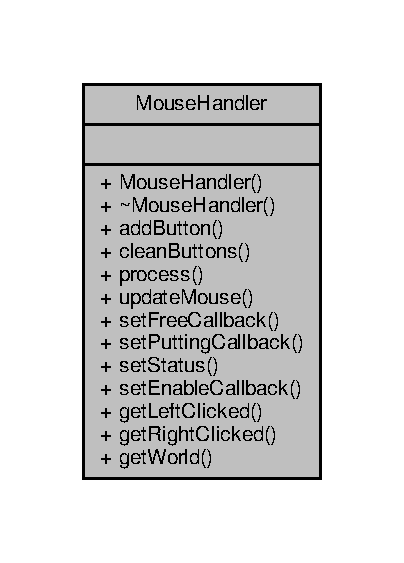
\includegraphics[height=550pt]{classMouseHandler__coll__graph}
\end{center}
\end{figure}
\subsection*{Public Types}
\begin{DoxyCompactItemize}
\item 
enum \hyperlink{classMouseHandler_af967315727aa1d435d55cc704e64fd1a}{Mouse\+Status} \{ \hyperlink{classMouseHandler_af967315727aa1d435d55cc704e64fd1aa5aba71e1304fdbe0f2899b6b1345d74a}{M\+O\+U\+S\+E\+\_\+\+F\+R\+E\+E} = 0, 
\hyperlink{classMouseHandler_af967315727aa1d435d55cc704e64fd1aa440928d86f44f388601ede4e6b91df76}{M\+O\+U\+S\+E\+\_\+\+P\+U\+T\+T\+I\+N\+G} = 1
 \}
\end{DoxyCompactItemize}
\subsection*{Public Member Functions}
\begin{DoxyCompactItemize}
\item 
\hyperlink{classMouseHandler_a2c79a128cb7e48f556cb228a3b14f291}{Mouse\+Handler} (\hyperlink{classWorld}{World} $\ast$\+\_\+world)
\item 
\hyperlink{classMouseHandler_a316de94666a31919abaadbb3ff16a18f}{$\sim$\+Mouse\+Handler} ()
\item 
void \hyperlink{classMouseHandler_a27fd9eb5eba52764d5ff6245018ee228}{add\+Button} (\hyperlink{classRigid}{Rigid} $\ast$\+\_\+rigid, \hyperlink{classMouseCallback}{Mouse\+Callback} $\ast$\+\_\+callback)
\begin{DoxyCompactList}\small\item\em add a button to the button list \end{DoxyCompactList}\item 
void \hyperlink{classMouseHandler_aece2b15ab5c31a8cc1befc5f18133f27}{clean\+Buttons} ()
\begin{DoxyCompactList}\small\item\em Clean all the buttons and delete the corresponding callbacks. \end{DoxyCompactList}\item 
void \hyperlink{classMouseHandler_a367ef9b85ee425a85beefdbd16a39768}{process} ()
\begin{DoxyCompactList}\small\item\em main entry to process \end{DoxyCompactList}\item 
void \hyperlink{classMouseHandler_a0a7df02e71fbbb14f5a80163ee065c8b}{update\+Mouse} ()
\begin{DoxyCompactList}\small\item\em update current mouse status from G\+L\+F\+W should be public for \hyperlink{classWorld}{World} to set it as friend \end{DoxyCompactList}\item 
void \hyperlink{classMouseHandler_a24de5aaed3df346eae098cd830f168dd}{set\+Free\+Callback} (\hyperlink{classMouseCallback}{Mouse\+Callback} $\ast$callback)
\begin{DoxyCompactList}\small\item\em Set callback that used at M\+O\+U\+S\+E\+\_\+\+F\+R\+E\+E when is not on buttons. \end{DoxyCompactList}\item 
void \hyperlink{classMouseHandler_a8b2e24e7199d4a33562c87b50f135fb2}{set\+Putting\+Callback} (\hyperlink{classMouseCallback}{Mouse\+Callback} $\ast$callback)
\begin{DoxyCompactList}\small\item\em Set callback that used at M\+O\+U\+S\+E\+\_\+\+P\+U\+T\+T\+I\+N\+G. \end{DoxyCompactList}\item 
void \hyperlink{classMouseHandler_a8f252c03ffcfe43b09086a9f5201792b}{set\+Status} (\hyperlink{classMouseHandler_af967315727aa1d435d55cc704e64fd1a}{Mouse\+Status} \+\_\+status, \hyperlink{classMouseCallback}{Mouse\+Callback} $\ast$callback=N\+U\+L\+L)
\begin{DoxyCompactList}\small\item\em set woring status callback used for corresponding status can be set through the 2nd parameter, O\+N\+L\+Y if it is not N\+U\+L\+L. \end{DoxyCompactList}\item 
void \hyperlink{classMouseHandler_a3a64869cf23c6d979ce6ac4a0127a93e}{set\+Enable\+Callback} (bool \+\_\+enable)
\begin{DoxyCompactList}\small\item\em Enable/disable all callbacks. \end{DoxyCompactList}\item 
bool \hyperlink{classMouseHandler_ae0bda6b1555601ea331951e813848260}{get\+Left\+Clicked} () const 
\item 
bool \hyperlink{classMouseHandler_ac94dc769799b712128bc6af848d187e3}{get\+Right\+Clicked} () const 
\item 
\hyperlink{classWorld}{World} $\ast$ \hyperlink{classMouseHandler_a35f26398677136e135a72286f40e7f61}{get\+World} () const 
\end{DoxyCompactItemize}
\subsection*{Private Member Functions}
\begin{DoxyCompactItemize}
\item 
void \hyperlink{classMouseHandler_aafb50967285e8c1a453d45c35f888810}{trigger\+Callback} (\hyperlink{classMouseCallback}{Mouse\+Callback} $\ast$callback)
\item 
void \hyperlink{classMouseHandler_ac065172398b09cf5823d2b5ae739e8e0}{process\+Free} ()
\item 
void \hyperlink{classMouseHandler_ad9b30d8f27f8aa35cb9e4afb47f2dca3}{process\+Putting} ()
\item 
void \hyperlink{classMouseHandler_a8ec027e132bbeae8afd7c9716c92631b}{reset} ()
\end{DoxyCompactItemize}
\subsection*{Private Attributes}
\begin{DoxyCompactItemize}
\item 
\hyperlink{classWorld}{World} $\ast$ \hyperlink{classMouseHandler_a90ecdcff9ced6f454c66cad224a1e914}{m\+World}
\item 
float \hyperlink{classMouseHandler_a410ce28feb21ea6f6426c9f96f9bba2f}{world\+X}
\item 
float \hyperlink{classMouseHandler_ab3a5274610896b90da3adf48345cfa3a}{world\+Y}
\item 
bool \hyperlink{classMouseHandler_ae6ab60c2b4761c3e90bfaab2e305e41e}{left\+Clicked}
\item 
bool \hyperlink{classMouseHandler_a0f6f7ab59e4ad42bcaf7e6549ff6566f}{right\+Clicked}
\item 
bool \hyperlink{classMouseHandler_a42f557e16701dab03efb4f99374ea524}{left\+Hold}
\item 
bool \hyperlink{classMouseHandler_af2f5a2328ceb7ba92728c71076ceb813}{right\+Hold}
\item 
bool \hyperlink{classMouseHandler_a34bc772a5e68fe68bb57ae495ef1fe69}{left\+Release}
\item 
bool \hyperlink{classMouseHandler_a53838184bd9bc307e5429b551f96c1ac}{right\+Release}
\item 
clock\+\_\+t \hyperlink{classMouseHandler_a6c3cee7fc0ca734bace60b951fb96b14}{last\+Clicked\+Clock}
\item 
\hyperlink{classMouseHandler_af967315727aa1d435d55cc704e64fd1a}{Mouse\+Status} \hyperlink{classMouseHandler_a34fd395066a9b32fe9a966ec4e1d5ea6}{status}
\item 
std\+::list$<$ std\+::pair$<$ \hyperlink{classRigid}{Rigid} $\ast$, \hyperlink{classMouseCallback}{Mouse\+Callback} $\ast$ $>$ $>$ \hyperlink{classMouseHandler_acfb0584232c1d5b8a87028d3008133e3}{buttons}
\item 
\hyperlink{classMouseCallback}{Mouse\+Callback} $\ast$ \hyperlink{classMouseHandler_a8e23b23bd4415cd057636573f6e8db30}{m\+Free\+Callback}
\item 
\hyperlink{classMouseCallback}{Mouse\+Callback} $\ast$ \hyperlink{classMouseHandler_a23f5b0cedc9e4c87060dcd3e10b943f4}{m\+Putting\+Callback}
\item 
bool \hyperlink{classMouseHandler_a29da34736a6d4f948a536f4d95bb146e}{enable\+Callback}
\end{DoxyCompactItemize}


\subsection{Detailed Description}
Forwards mouse actions to \hyperlink{classMatter}{Matter}. 

\subsection{Member Enumeration Documentation}
\hypertarget{classMouseHandler_af967315727aa1d435d55cc704e64fd1a}{}\index{Mouse\+Handler@{Mouse\+Handler}!Mouse\+Status@{Mouse\+Status}}
\index{Mouse\+Status@{Mouse\+Status}!Mouse\+Handler@{Mouse\+Handler}}
\subsubsection[{Mouse\+Status}]{\setlength{\rightskip}{0pt plus 5cm}enum {\bf Mouse\+Handler\+::\+Mouse\+Status}}\label{classMouseHandler_af967315727aa1d435d55cc704e64fd1a}
\begin{Desc}
\item[Enumerator]\par
\begin{description}
\index{M\+O\+U\+S\+E\+\_\+\+F\+R\+E\+E@{M\+O\+U\+S\+E\+\_\+\+F\+R\+E\+E}!Mouse\+Handler@{Mouse\+Handler}}\index{Mouse\+Handler@{Mouse\+Handler}!M\+O\+U\+S\+E\+\_\+\+F\+R\+E\+E@{M\+O\+U\+S\+E\+\_\+\+F\+R\+E\+E}}\item[{\em 
\hypertarget{classMouseHandler_af967315727aa1d435d55cc704e64fd1aa5aba71e1304fdbe0f2899b6b1345d74a}{}M\+O\+U\+S\+E\+\_\+\+F\+R\+E\+E\label{classMouseHandler_af967315727aa1d435d55cc704e64fd1aa5aba71e1304fdbe0f2899b6b1345d74a}
}]\index{M\+O\+U\+S\+E\+\_\+\+P\+U\+T\+T\+I\+N\+G@{M\+O\+U\+S\+E\+\_\+\+P\+U\+T\+T\+I\+N\+G}!Mouse\+Handler@{Mouse\+Handler}}\index{Mouse\+Handler@{Mouse\+Handler}!M\+O\+U\+S\+E\+\_\+\+P\+U\+T\+T\+I\+N\+G@{M\+O\+U\+S\+E\+\_\+\+P\+U\+T\+T\+I\+N\+G}}\item[{\em 
\hypertarget{classMouseHandler_af967315727aa1d435d55cc704e64fd1aa440928d86f44f388601ede4e6b91df76}{}M\+O\+U\+S\+E\+\_\+\+P\+U\+T\+T\+I\+N\+G\label{classMouseHandler_af967315727aa1d435d55cc704e64fd1aa440928d86f44f388601ede4e6b91df76}
}]\end{description}
\end{Desc}


\subsection{Constructor \& Destructor Documentation}
\hypertarget{classMouseHandler_a2c79a128cb7e48f556cb228a3b14f291}{}\index{Mouse\+Handler@{Mouse\+Handler}!Mouse\+Handler@{Mouse\+Handler}}
\index{Mouse\+Handler@{Mouse\+Handler}!Mouse\+Handler@{Mouse\+Handler}}
\subsubsection[{Mouse\+Handler}]{\setlength{\rightskip}{0pt plus 5cm}Mouse\+Handler\+::\+Mouse\+Handler (
\begin{DoxyParamCaption}
\item[{{\bf World} $\ast$}]{\+\_\+world}
\end{DoxyParamCaption}
)}\label{classMouseHandler_a2c79a128cb7e48f556cb228a3b14f291}
\hypertarget{classMouseHandler_a316de94666a31919abaadbb3ff16a18f}{}\index{Mouse\+Handler@{Mouse\+Handler}!````~Mouse\+Handler@{$\sim$\+Mouse\+Handler}}
\index{````~Mouse\+Handler@{$\sim$\+Mouse\+Handler}!Mouse\+Handler@{Mouse\+Handler}}
\subsubsection[{$\sim$\+Mouse\+Handler}]{\setlength{\rightskip}{0pt plus 5cm}Mouse\+Handler\+::$\sim$\+Mouse\+Handler (
\begin{DoxyParamCaption}
{}
\end{DoxyParamCaption}
)}\label{classMouseHandler_a316de94666a31919abaadbb3ff16a18f}


\subsection{Member Function Documentation}
\hypertarget{classMouseHandler_a27fd9eb5eba52764d5ff6245018ee228}{}\index{Mouse\+Handler@{Mouse\+Handler}!add\+Button@{add\+Button}}
\index{add\+Button@{add\+Button}!Mouse\+Handler@{Mouse\+Handler}}
\subsubsection[{add\+Button}]{\setlength{\rightskip}{0pt plus 5cm}void Mouse\+Handler\+::add\+Button (
\begin{DoxyParamCaption}
\item[{{\bf Rigid} $\ast$}]{\+\_\+rigid, }
\item[{{\bf Mouse\+Callback} $\ast$}]{\+\_\+callback}
\end{DoxyParamCaption}
)}\label{classMouseHandler_a27fd9eb5eba52764d5ff6245018ee228}


add a button to the button list 

\hypertarget{classMouseHandler_aece2b15ab5c31a8cc1befc5f18133f27}{}\index{Mouse\+Handler@{Mouse\+Handler}!clean\+Buttons@{clean\+Buttons}}
\index{clean\+Buttons@{clean\+Buttons}!Mouse\+Handler@{Mouse\+Handler}}
\subsubsection[{clean\+Buttons}]{\setlength{\rightskip}{0pt plus 5cm}void Mouse\+Handler\+::clean\+Buttons (
\begin{DoxyParamCaption}
{}
\end{DoxyParamCaption}
)}\label{classMouseHandler_aece2b15ab5c31a8cc1befc5f18133f27}


Clean all the buttons and delete the corresponding callbacks. 

\hypertarget{classMouseHandler_ae0bda6b1555601ea331951e813848260}{}\index{Mouse\+Handler@{Mouse\+Handler}!get\+Left\+Clicked@{get\+Left\+Clicked}}
\index{get\+Left\+Clicked@{get\+Left\+Clicked}!Mouse\+Handler@{Mouse\+Handler}}
\subsubsection[{get\+Left\+Clicked}]{\setlength{\rightskip}{0pt plus 5cm}bool Mouse\+Handler\+::get\+Left\+Clicked (
\begin{DoxyParamCaption}
{}
\end{DoxyParamCaption}
) const\hspace{0.3cm}{\ttfamily [inline]}}\label{classMouseHandler_ae0bda6b1555601ea331951e813848260}
\hypertarget{classMouseHandler_ac94dc769799b712128bc6af848d187e3}{}\index{Mouse\+Handler@{Mouse\+Handler}!get\+Right\+Clicked@{get\+Right\+Clicked}}
\index{get\+Right\+Clicked@{get\+Right\+Clicked}!Mouse\+Handler@{Mouse\+Handler}}
\subsubsection[{get\+Right\+Clicked}]{\setlength{\rightskip}{0pt plus 5cm}bool Mouse\+Handler\+::get\+Right\+Clicked (
\begin{DoxyParamCaption}
{}
\end{DoxyParamCaption}
) const\hspace{0.3cm}{\ttfamily [inline]}}\label{classMouseHandler_ac94dc769799b712128bc6af848d187e3}
\hypertarget{classMouseHandler_a35f26398677136e135a72286f40e7f61}{}\index{Mouse\+Handler@{Mouse\+Handler}!get\+World@{get\+World}}
\index{get\+World@{get\+World}!Mouse\+Handler@{Mouse\+Handler}}
\subsubsection[{get\+World}]{\setlength{\rightskip}{0pt plus 5cm}{\bf World}$\ast$ Mouse\+Handler\+::get\+World (
\begin{DoxyParamCaption}
{}
\end{DoxyParamCaption}
) const\hspace{0.3cm}{\ttfamily [inline]}}\label{classMouseHandler_a35f26398677136e135a72286f40e7f61}
\hypertarget{classMouseHandler_a367ef9b85ee425a85beefdbd16a39768}{}\index{Mouse\+Handler@{Mouse\+Handler}!process@{process}}
\index{process@{process}!Mouse\+Handler@{Mouse\+Handler}}
\subsubsection[{process}]{\setlength{\rightskip}{0pt plus 5cm}void Mouse\+Handler\+::process (
\begin{DoxyParamCaption}
{}
\end{DoxyParamCaption}
)}\label{classMouseHandler_a367ef9b85ee425a85beefdbd16a39768}


main entry to process 

\hypertarget{classMouseHandler_ac065172398b09cf5823d2b5ae739e8e0}{}\index{Mouse\+Handler@{Mouse\+Handler}!process\+Free@{process\+Free}}
\index{process\+Free@{process\+Free}!Mouse\+Handler@{Mouse\+Handler}}
\subsubsection[{process\+Free}]{\setlength{\rightskip}{0pt plus 5cm}void Mouse\+Handler\+::process\+Free (
\begin{DoxyParamCaption}
{}
\end{DoxyParamCaption}
)\hspace{0.3cm}{\ttfamily [private]}}\label{classMouseHandler_ac065172398b09cf5823d2b5ae739e8e0}
\hypertarget{classMouseHandler_ad9b30d8f27f8aa35cb9e4afb47f2dca3}{}\index{Mouse\+Handler@{Mouse\+Handler}!process\+Putting@{process\+Putting}}
\index{process\+Putting@{process\+Putting}!Mouse\+Handler@{Mouse\+Handler}}
\subsubsection[{process\+Putting}]{\setlength{\rightskip}{0pt plus 5cm}void Mouse\+Handler\+::process\+Putting (
\begin{DoxyParamCaption}
{}
\end{DoxyParamCaption}
)\hspace{0.3cm}{\ttfamily [private]}}\label{classMouseHandler_ad9b30d8f27f8aa35cb9e4afb47f2dca3}
\hypertarget{classMouseHandler_a8ec027e132bbeae8afd7c9716c92631b}{}\index{Mouse\+Handler@{Mouse\+Handler}!reset@{reset}}
\index{reset@{reset}!Mouse\+Handler@{Mouse\+Handler}}
\subsubsection[{reset}]{\setlength{\rightskip}{0pt plus 5cm}void Mouse\+Handler\+::reset (
\begin{DoxyParamCaption}
{}
\end{DoxyParamCaption}
)\hspace{0.3cm}{\ttfamily [private]}}\label{classMouseHandler_a8ec027e132bbeae8afd7c9716c92631b}
\hypertarget{classMouseHandler_a3a64869cf23c6d979ce6ac4a0127a93e}{}\index{Mouse\+Handler@{Mouse\+Handler}!set\+Enable\+Callback@{set\+Enable\+Callback}}
\index{set\+Enable\+Callback@{set\+Enable\+Callback}!Mouse\+Handler@{Mouse\+Handler}}
\subsubsection[{set\+Enable\+Callback}]{\setlength{\rightskip}{0pt plus 5cm}void Mouse\+Handler\+::set\+Enable\+Callback (
\begin{DoxyParamCaption}
\item[{bool}]{\+\_\+enable}
\end{DoxyParamCaption}
)\hspace{0.3cm}{\ttfamily [inline]}}\label{classMouseHandler_a3a64869cf23c6d979ce6ac4a0127a93e}


Enable/disable all callbacks. 

\hypertarget{classMouseHandler_a24de5aaed3df346eae098cd830f168dd}{}\index{Mouse\+Handler@{Mouse\+Handler}!set\+Free\+Callback@{set\+Free\+Callback}}
\index{set\+Free\+Callback@{set\+Free\+Callback}!Mouse\+Handler@{Mouse\+Handler}}
\subsubsection[{set\+Free\+Callback}]{\setlength{\rightskip}{0pt plus 5cm}void Mouse\+Handler\+::set\+Free\+Callback (
\begin{DoxyParamCaption}
\item[{{\bf Mouse\+Callback} $\ast$}]{callback}
\end{DoxyParamCaption}
)}\label{classMouseHandler_a24de5aaed3df346eae098cd830f168dd}


Set callback that used at M\+O\+U\+S\+E\+\_\+\+F\+R\+E\+E when is not on buttons. 

This callback will N\+O\+T be deleted when switching status. \hypertarget{classMouseHandler_a8b2e24e7199d4a33562c87b50f135fb2}{}\index{Mouse\+Handler@{Mouse\+Handler}!set\+Putting\+Callback@{set\+Putting\+Callback}}
\index{set\+Putting\+Callback@{set\+Putting\+Callback}!Mouse\+Handler@{Mouse\+Handler}}
\subsubsection[{set\+Putting\+Callback}]{\setlength{\rightskip}{0pt plus 5cm}void Mouse\+Handler\+::set\+Putting\+Callback (
\begin{DoxyParamCaption}
\item[{{\bf Mouse\+Callback} $\ast$}]{callback}
\end{DoxyParamCaption}
)}\label{classMouseHandler_a8b2e24e7199d4a33562c87b50f135fb2}


Set callback that used at M\+O\+U\+S\+E\+\_\+\+P\+U\+T\+T\+I\+N\+G. 

This callback will be deleted when switching status. \hypertarget{classMouseHandler_a8f252c03ffcfe43b09086a9f5201792b}{}\index{Mouse\+Handler@{Mouse\+Handler}!set\+Status@{set\+Status}}
\index{set\+Status@{set\+Status}!Mouse\+Handler@{Mouse\+Handler}}
\subsubsection[{set\+Status}]{\setlength{\rightskip}{0pt plus 5cm}void Mouse\+Handler\+::set\+Status (
\begin{DoxyParamCaption}
\item[{{\bf Mouse\+Status}}]{\+\_\+status, }
\item[{{\bf Mouse\+Callback} $\ast$}]{callback = {\ttfamily NULL}}
\end{DoxyParamCaption}
)}\label{classMouseHandler_a8f252c03ffcfe43b09086a9f5201792b}


set woring status callback used for corresponding status can be set through the 2nd parameter, O\+N\+L\+Y if it is not N\+U\+L\+L. 

\hypertarget{classMouseHandler_aafb50967285e8c1a453d45c35f888810}{}\index{Mouse\+Handler@{Mouse\+Handler}!trigger\+Callback@{trigger\+Callback}}
\index{trigger\+Callback@{trigger\+Callback}!Mouse\+Handler@{Mouse\+Handler}}
\subsubsection[{trigger\+Callback}]{\setlength{\rightskip}{0pt plus 5cm}void Mouse\+Handler\+::trigger\+Callback (
\begin{DoxyParamCaption}
\item[{{\bf Mouse\+Callback} $\ast$}]{callback}
\end{DoxyParamCaption}
)\hspace{0.3cm}{\ttfamily [private]}}\label{classMouseHandler_aafb50967285e8c1a453d45c35f888810}
\hypertarget{classMouseHandler_a0a7df02e71fbbb14f5a80163ee065c8b}{}\index{Mouse\+Handler@{Mouse\+Handler}!update\+Mouse@{update\+Mouse}}
\index{update\+Mouse@{update\+Mouse}!Mouse\+Handler@{Mouse\+Handler}}
\subsubsection[{update\+Mouse}]{\setlength{\rightskip}{0pt plus 5cm}void Mouse\+Handler\+::update\+Mouse (
\begin{DoxyParamCaption}
{}
\end{DoxyParamCaption}
)}\label{classMouseHandler_a0a7df02e71fbbb14f5a80163ee065c8b}


update current mouse status from G\+L\+F\+W should be public for \hyperlink{classWorld}{World} to set it as friend 



\subsection{Member Data Documentation}
\hypertarget{classMouseHandler_acfb0584232c1d5b8a87028d3008133e3}{}\index{Mouse\+Handler@{Mouse\+Handler}!buttons@{buttons}}
\index{buttons@{buttons}!Mouse\+Handler@{Mouse\+Handler}}
\subsubsection[{buttons}]{\setlength{\rightskip}{0pt plus 5cm}std\+::list$<$ std\+::pair$<${\bf Rigid}$\ast$, {\bf Mouse\+Callback}$\ast$$>$ $>$ Mouse\+Handler\+::buttons\hspace{0.3cm}{\ttfamily [private]}}\label{classMouseHandler_acfb0584232c1d5b8a87028d3008133e3}
\hypertarget{classMouseHandler_a29da34736a6d4f948a536f4d95bb146e}{}\index{Mouse\+Handler@{Mouse\+Handler}!enable\+Callback@{enable\+Callback}}
\index{enable\+Callback@{enable\+Callback}!Mouse\+Handler@{Mouse\+Handler}}
\subsubsection[{enable\+Callback}]{\setlength{\rightskip}{0pt plus 5cm}bool Mouse\+Handler\+::enable\+Callback\hspace{0.3cm}{\ttfamily [private]}}\label{classMouseHandler_a29da34736a6d4f948a536f4d95bb146e}
\hypertarget{classMouseHandler_a6c3cee7fc0ca734bace60b951fb96b14}{}\index{Mouse\+Handler@{Mouse\+Handler}!last\+Clicked\+Clock@{last\+Clicked\+Clock}}
\index{last\+Clicked\+Clock@{last\+Clicked\+Clock}!Mouse\+Handler@{Mouse\+Handler}}
\subsubsection[{last\+Clicked\+Clock}]{\setlength{\rightskip}{0pt plus 5cm}clock\+\_\+t Mouse\+Handler\+::last\+Clicked\+Clock\hspace{0.3cm}{\ttfamily [private]}}\label{classMouseHandler_a6c3cee7fc0ca734bace60b951fb96b14}
\hypertarget{classMouseHandler_ae6ab60c2b4761c3e90bfaab2e305e41e}{}\index{Mouse\+Handler@{Mouse\+Handler}!left\+Clicked@{left\+Clicked}}
\index{left\+Clicked@{left\+Clicked}!Mouse\+Handler@{Mouse\+Handler}}
\subsubsection[{left\+Clicked}]{\setlength{\rightskip}{0pt plus 5cm}bool Mouse\+Handler\+::left\+Clicked\hspace{0.3cm}{\ttfamily [private]}}\label{classMouseHandler_ae6ab60c2b4761c3e90bfaab2e305e41e}
\hypertarget{classMouseHandler_a42f557e16701dab03efb4f99374ea524}{}\index{Mouse\+Handler@{Mouse\+Handler}!left\+Hold@{left\+Hold}}
\index{left\+Hold@{left\+Hold}!Mouse\+Handler@{Mouse\+Handler}}
\subsubsection[{left\+Hold}]{\setlength{\rightskip}{0pt plus 5cm}bool Mouse\+Handler\+::left\+Hold\hspace{0.3cm}{\ttfamily [private]}}\label{classMouseHandler_a42f557e16701dab03efb4f99374ea524}
\hypertarget{classMouseHandler_a34bc772a5e68fe68bb57ae495ef1fe69}{}\index{Mouse\+Handler@{Mouse\+Handler}!left\+Release@{left\+Release}}
\index{left\+Release@{left\+Release}!Mouse\+Handler@{Mouse\+Handler}}
\subsubsection[{left\+Release}]{\setlength{\rightskip}{0pt plus 5cm}bool Mouse\+Handler\+::left\+Release\hspace{0.3cm}{\ttfamily [private]}}\label{classMouseHandler_a34bc772a5e68fe68bb57ae495ef1fe69}
\hypertarget{classMouseHandler_a8e23b23bd4415cd057636573f6e8db30}{}\index{Mouse\+Handler@{Mouse\+Handler}!m\+Free\+Callback@{m\+Free\+Callback}}
\index{m\+Free\+Callback@{m\+Free\+Callback}!Mouse\+Handler@{Mouse\+Handler}}
\subsubsection[{m\+Free\+Callback}]{\setlength{\rightskip}{0pt plus 5cm}{\bf Mouse\+Callback}$\ast$ Mouse\+Handler\+::m\+Free\+Callback\hspace{0.3cm}{\ttfamily [private]}}\label{classMouseHandler_a8e23b23bd4415cd057636573f6e8db30}
\hypertarget{classMouseHandler_a23f5b0cedc9e4c87060dcd3e10b943f4}{}\index{Mouse\+Handler@{Mouse\+Handler}!m\+Putting\+Callback@{m\+Putting\+Callback}}
\index{m\+Putting\+Callback@{m\+Putting\+Callback}!Mouse\+Handler@{Mouse\+Handler}}
\subsubsection[{m\+Putting\+Callback}]{\setlength{\rightskip}{0pt plus 5cm}{\bf Mouse\+Callback} $\ast$ Mouse\+Handler\+::m\+Putting\+Callback\hspace{0.3cm}{\ttfamily [private]}}\label{classMouseHandler_a23f5b0cedc9e4c87060dcd3e10b943f4}
\hypertarget{classMouseHandler_a90ecdcff9ced6f454c66cad224a1e914}{}\index{Mouse\+Handler@{Mouse\+Handler}!m\+World@{m\+World}}
\index{m\+World@{m\+World}!Mouse\+Handler@{Mouse\+Handler}}
\subsubsection[{m\+World}]{\setlength{\rightskip}{0pt plus 5cm}{\bf World}$\ast$ Mouse\+Handler\+::m\+World\hspace{0.3cm}{\ttfamily [private]}}\label{classMouseHandler_a90ecdcff9ced6f454c66cad224a1e914}
\hypertarget{classMouseHandler_a0f6f7ab59e4ad42bcaf7e6549ff6566f}{}\index{Mouse\+Handler@{Mouse\+Handler}!right\+Clicked@{right\+Clicked}}
\index{right\+Clicked@{right\+Clicked}!Mouse\+Handler@{Mouse\+Handler}}
\subsubsection[{right\+Clicked}]{\setlength{\rightskip}{0pt plus 5cm}bool Mouse\+Handler\+::right\+Clicked\hspace{0.3cm}{\ttfamily [private]}}\label{classMouseHandler_a0f6f7ab59e4ad42bcaf7e6549ff6566f}
\hypertarget{classMouseHandler_af2f5a2328ceb7ba92728c71076ceb813}{}\index{Mouse\+Handler@{Mouse\+Handler}!right\+Hold@{right\+Hold}}
\index{right\+Hold@{right\+Hold}!Mouse\+Handler@{Mouse\+Handler}}
\subsubsection[{right\+Hold}]{\setlength{\rightskip}{0pt plus 5cm}bool Mouse\+Handler\+::right\+Hold\hspace{0.3cm}{\ttfamily [private]}}\label{classMouseHandler_af2f5a2328ceb7ba92728c71076ceb813}
\hypertarget{classMouseHandler_a53838184bd9bc307e5429b551f96c1ac}{}\index{Mouse\+Handler@{Mouse\+Handler}!right\+Release@{right\+Release}}
\index{right\+Release@{right\+Release}!Mouse\+Handler@{Mouse\+Handler}}
\subsubsection[{right\+Release}]{\setlength{\rightskip}{0pt plus 5cm}bool Mouse\+Handler\+::right\+Release\hspace{0.3cm}{\ttfamily [private]}}\label{classMouseHandler_a53838184bd9bc307e5429b551f96c1ac}
\hypertarget{classMouseHandler_a34fd395066a9b32fe9a966ec4e1d5ea6}{}\index{Mouse\+Handler@{Mouse\+Handler}!status@{status}}
\index{status@{status}!Mouse\+Handler@{Mouse\+Handler}}
\subsubsection[{status}]{\setlength{\rightskip}{0pt plus 5cm}{\bf Mouse\+Status} Mouse\+Handler\+::status\hspace{0.3cm}{\ttfamily [private]}}\label{classMouseHandler_a34fd395066a9b32fe9a966ec4e1d5ea6}
\hypertarget{classMouseHandler_a410ce28feb21ea6f6426c9f96f9bba2f}{}\index{Mouse\+Handler@{Mouse\+Handler}!world\+X@{world\+X}}
\index{world\+X@{world\+X}!Mouse\+Handler@{Mouse\+Handler}}
\subsubsection[{world\+X}]{\setlength{\rightskip}{0pt plus 5cm}float Mouse\+Handler\+::world\+X\hspace{0.3cm}{\ttfamily [private]}}\label{classMouseHandler_a410ce28feb21ea6f6426c9f96f9bba2f}
\hypertarget{classMouseHandler_ab3a5274610896b90da3adf48345cfa3a}{}\index{Mouse\+Handler@{Mouse\+Handler}!world\+Y@{world\+Y}}
\index{world\+Y@{world\+Y}!Mouse\+Handler@{Mouse\+Handler}}
\subsubsection[{world\+Y}]{\setlength{\rightskip}{0pt plus 5cm}float Mouse\+Handler\+::world\+Y\hspace{0.3cm}{\ttfamily [private]}}\label{classMouseHandler_ab3a5274610896b90da3adf48345cfa3a}


The documentation for this class was generated from the following files\+:\begin{DoxyCompactItemize}
\item 
\hyperlink{mousehandler_8h}{mousehandler.\+h}\item 
\hyperlink{mousehandler_8cpp}{mousehandler.\+cpp}\end{DoxyCompactItemize}

\hypertarget{classWorld_1_1MyContactListener}{}\section{World\+:\+:My\+Contact\+Listener Class Reference}
\label{classWorld_1_1MyContactListener}\index{World\+::\+My\+Contact\+Listener@{World\+::\+My\+Contact\+Listener}}


Inheritance diagram for World\+:\+:My\+Contact\+Listener\+:
\nopagebreak
\begin{figure}[H]
\begin{center}
\leavevmode
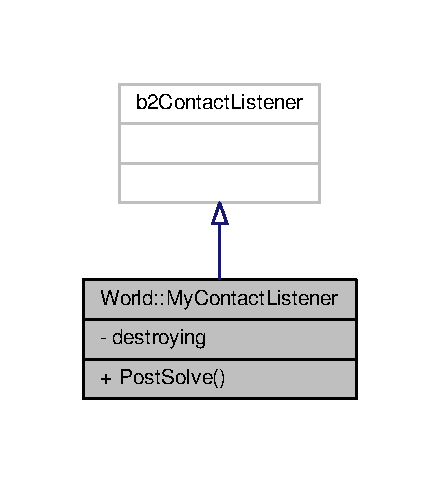
\includegraphics[width=211pt]{classWorld_1_1MyContactListener__inherit__graph}
\end{center}
\end{figure}


Collaboration diagram for World\+:\+:My\+Contact\+Listener\+:
\nopagebreak
\begin{figure}[H]
\begin{center}
\leavevmode
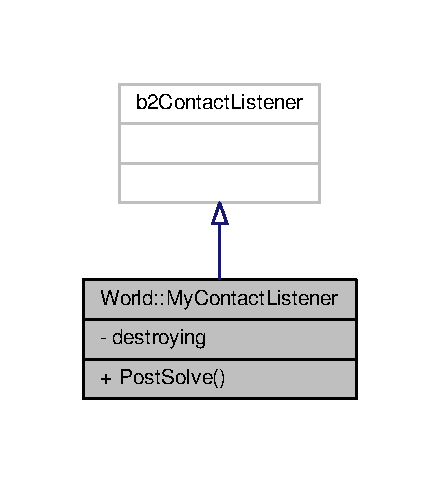
\includegraphics[width=211pt]{classWorld_1_1MyContactListener__coll__graph}
\end{center}
\end{figure}
\subsection*{Public Member Functions}
\begin{DoxyCompactItemize}
\item 
void \hyperlink{classWorld_1_1MyContactListener_abc23035ab45a8a0fb4ea605a866e360d}{Post\+Solve} (b2\+Contact $\ast$contact, const b2\+Contact\+Impulse $\ast$impulse) override
\end{DoxyCompactItemize}
\subsection*{Private Attributes}
\begin{DoxyCompactItemize}
\item 
std\+::vector$<$ \hyperlink{classRigid}{Rigid} $\ast$ $>$ \hyperlink{classWorld_1_1MyContactListener_ac21436147cb87aeca120c614df96d8b8}{destroying}
\end{DoxyCompactItemize}
\subsection*{Friends}
\begin{DoxyCompactItemize}
\item 
void \hyperlink{classWorld_1_1MyContactListener_ab41dd1d2a31468cdcba23838de4fd474}{World\+::exam\+Contact} ()
\end{DoxyCompactItemize}


\subsection{Member Function Documentation}
\hypertarget{classWorld_1_1MyContactListener_abc23035ab45a8a0fb4ea605a866e360d}{}\index{World\+::\+My\+Contact\+Listener@{World\+::\+My\+Contact\+Listener}!Post\+Solve@{Post\+Solve}}
\index{Post\+Solve@{Post\+Solve}!World\+::\+My\+Contact\+Listener@{World\+::\+My\+Contact\+Listener}}
\subsubsection[{Post\+Solve}]{\setlength{\rightskip}{0pt plus 5cm}void World\+::\+My\+Contact\+Listener\+::\+Post\+Solve (
\begin{DoxyParamCaption}
\item[{b2\+Contact $\ast$}]{contact, }
\item[{const b2\+Contact\+Impulse $\ast$}]{impulse}
\end{DoxyParamCaption}
)\hspace{0.3cm}{\ttfamily [override]}}\label{classWorld_1_1MyContactListener_abc23035ab45a8a0fb4ea605a866e360d}


\subsection{Friends And Related Function Documentation}
\hypertarget{classWorld_1_1MyContactListener_ab41dd1d2a31468cdcba23838de4fd474}{}\index{World\+::\+My\+Contact\+Listener@{World\+::\+My\+Contact\+Listener}!World\+::exam\+Contact@{World\+::exam\+Contact}}
\index{World\+::exam\+Contact@{World\+::exam\+Contact}!World\+::\+My\+Contact\+Listener@{World\+::\+My\+Contact\+Listener}}
\subsubsection[{World\+::exam\+Contact}]{\setlength{\rightskip}{0pt plus 5cm}void {\bf World\+::exam\+Contact} (
\begin{DoxyParamCaption}
{}
\end{DoxyParamCaption}
)\hspace{0.3cm}{\ttfamily [friend]}}\label{classWorld_1_1MyContactListener_ab41dd1d2a31468cdcba23838de4fd474}


\subsection{Member Data Documentation}
\hypertarget{classWorld_1_1MyContactListener_ac21436147cb87aeca120c614df96d8b8}{}\index{World\+::\+My\+Contact\+Listener@{World\+::\+My\+Contact\+Listener}!destroying@{destroying}}
\index{destroying@{destroying}!World\+::\+My\+Contact\+Listener@{World\+::\+My\+Contact\+Listener}}
\subsubsection[{destroying}]{\setlength{\rightskip}{0pt plus 5cm}std\+::vector$<${\bf Rigid}$\ast$$>$ World\+::\+My\+Contact\+Listener\+::destroying\hspace{0.3cm}{\ttfamily [private]}}\label{classWorld_1_1MyContactListener_ac21436147cb87aeca120c614df96d8b8}


The documentation for this class was generated from the following files\+:\begin{DoxyCompactItemize}
\item 
\hyperlink{world_8h}{world.\+h}\item 
\hyperlink{world_8cpp}{world.\+cpp}\end{DoxyCompactItemize}

\hypertarget{classWorld_1_1MyDestructionListener}{}\section{World\+:\+:My\+Destruction\+Listener Class Reference}
\label{classWorld_1_1MyDestructionListener}\index{World\+::\+My\+Destruction\+Listener@{World\+::\+My\+Destruction\+Listener}}


Manger for all destruction listener.  




{\ttfamily \#include $<$world.\+h$>$}



Inheritance diagram for World\+:\+:My\+Destruction\+Listener\+:
\nopagebreak
\begin{figure}[H]
\begin{center}
\leavevmode
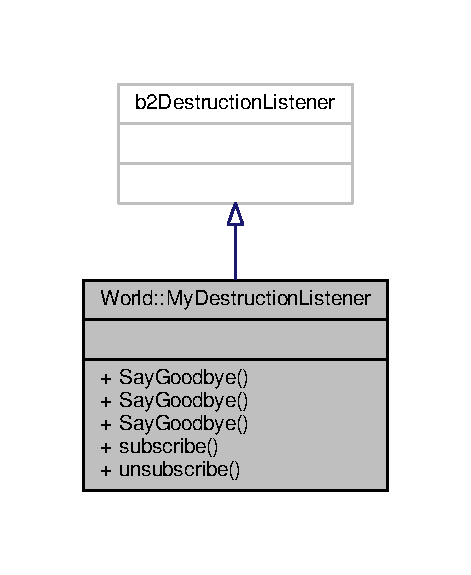
\includegraphics[width=226pt]{classWorld_1_1MyDestructionListener__inherit__graph}
\end{center}
\end{figure}


Collaboration diagram for World\+:\+:My\+Destruction\+Listener\+:
\nopagebreak
\begin{figure}[H]
\begin{center}
\leavevmode
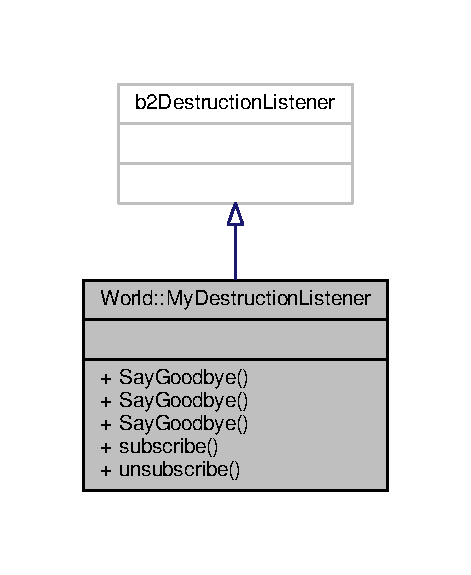
\includegraphics[width=226pt]{classWorld_1_1MyDestructionListener__coll__graph}
\end{center}
\end{figure}
\subsection*{Public Member Functions}
\begin{DoxyCompactItemize}
\item 
void \hyperlink{classWorld_1_1MyDestructionListener_afb69a87d5d2bfea63bb9fed16e6b6677}{Say\+Goodbye} (b2\+Joint $\ast$joint) override
\item 
void \hyperlink{classWorld_1_1MyDestructionListener_abf208c075a30abc88da5d8d91378de9a}{Say\+Goodbye} (b2\+Fixture $\ast$fixture) override
\item 
void \hyperlink{classWorld_1_1MyDestructionListener_a1cabe04394a461a952bbf027157b9628}{Say\+Goodbye} (b2\+Particle\+Group $\ast$group) override
\item 
void \hyperlink{classWorld_1_1MyDestructionListener_ac01b1f54aed1b55c959a2e58f21a0017}{subscribe} (b2\+Destruction\+Listener $\ast$p)
\item 
void \hyperlink{classWorld_1_1MyDestructionListener_a6304a373d6d6119737802b0d3916c977}{unsubscribe} (b2\+Destruction\+Listener $\ast$p)
\end{DoxyCompactItemize}
\subsection*{Private Attributes}
\begin{DoxyCompactItemize}
\item 
std\+::list$<$ b2\+Destruction\+Listener $\ast$ $>$ \hyperlink{classWorld_1_1MyDestructionListener_abae6aedcdb7b1fec3d4bab40621a0619}{subscribers}
\end{DoxyCompactItemize}


\subsection{Detailed Description}
Manger for all destruction listener. 

\subsection{Member Function Documentation}
\hypertarget{classWorld_1_1MyDestructionListener_afb69a87d5d2bfea63bb9fed16e6b6677}{}\index{World\+::\+My\+Destruction\+Listener@{World\+::\+My\+Destruction\+Listener}!Say\+Goodbye@{Say\+Goodbye}}
\index{Say\+Goodbye@{Say\+Goodbye}!World\+::\+My\+Destruction\+Listener@{World\+::\+My\+Destruction\+Listener}}
\subsubsection[{Say\+Goodbye}]{\setlength{\rightskip}{0pt plus 5cm}void World\+::\+My\+Destruction\+Listener\+::\+Say\+Goodbye (
\begin{DoxyParamCaption}
\item[{b2\+Joint $\ast$}]{joint}
\end{DoxyParamCaption}
)\hspace{0.3cm}{\ttfamily [override]}}\label{classWorld_1_1MyDestructionListener_afb69a87d5d2bfea63bb9fed16e6b6677}
\hypertarget{classWorld_1_1MyDestructionListener_abf208c075a30abc88da5d8d91378de9a}{}\index{World\+::\+My\+Destruction\+Listener@{World\+::\+My\+Destruction\+Listener}!Say\+Goodbye@{Say\+Goodbye}}
\index{Say\+Goodbye@{Say\+Goodbye}!World\+::\+My\+Destruction\+Listener@{World\+::\+My\+Destruction\+Listener}}
\subsubsection[{Say\+Goodbye}]{\setlength{\rightskip}{0pt plus 5cm}void World\+::\+My\+Destruction\+Listener\+::\+Say\+Goodbye (
\begin{DoxyParamCaption}
\item[{b2\+Fixture $\ast$}]{fixture}
\end{DoxyParamCaption}
)\hspace{0.3cm}{\ttfamily [override]}}\label{classWorld_1_1MyDestructionListener_abf208c075a30abc88da5d8d91378de9a}
\hypertarget{classWorld_1_1MyDestructionListener_a1cabe04394a461a952bbf027157b9628}{}\index{World\+::\+My\+Destruction\+Listener@{World\+::\+My\+Destruction\+Listener}!Say\+Goodbye@{Say\+Goodbye}}
\index{Say\+Goodbye@{Say\+Goodbye}!World\+::\+My\+Destruction\+Listener@{World\+::\+My\+Destruction\+Listener}}
\subsubsection[{Say\+Goodbye}]{\setlength{\rightskip}{0pt plus 5cm}void World\+::\+My\+Destruction\+Listener\+::\+Say\+Goodbye (
\begin{DoxyParamCaption}
\item[{b2\+Particle\+Group $\ast$}]{group}
\end{DoxyParamCaption}
)\hspace{0.3cm}{\ttfamily [override]}}\label{classWorld_1_1MyDestructionListener_a1cabe04394a461a952bbf027157b9628}
\hypertarget{classWorld_1_1MyDestructionListener_ac01b1f54aed1b55c959a2e58f21a0017}{}\index{World\+::\+My\+Destruction\+Listener@{World\+::\+My\+Destruction\+Listener}!subscribe@{subscribe}}
\index{subscribe@{subscribe}!World\+::\+My\+Destruction\+Listener@{World\+::\+My\+Destruction\+Listener}}
\subsubsection[{subscribe}]{\setlength{\rightskip}{0pt plus 5cm}void World\+::\+My\+Destruction\+Listener\+::subscribe (
\begin{DoxyParamCaption}
\item[{b2\+Destruction\+Listener $\ast$}]{p}
\end{DoxyParamCaption}
)}\label{classWorld_1_1MyDestructionListener_ac01b1f54aed1b55c959a2e58f21a0017}
\hypertarget{classWorld_1_1MyDestructionListener_a6304a373d6d6119737802b0d3916c977}{}\index{World\+::\+My\+Destruction\+Listener@{World\+::\+My\+Destruction\+Listener}!unsubscribe@{unsubscribe}}
\index{unsubscribe@{unsubscribe}!World\+::\+My\+Destruction\+Listener@{World\+::\+My\+Destruction\+Listener}}
\subsubsection[{unsubscribe}]{\setlength{\rightskip}{0pt plus 5cm}void World\+::\+My\+Destruction\+Listener\+::unsubscribe (
\begin{DoxyParamCaption}
\item[{b2\+Destruction\+Listener $\ast$}]{p}
\end{DoxyParamCaption}
)}\label{classWorld_1_1MyDestructionListener_a6304a373d6d6119737802b0d3916c977}


\subsection{Member Data Documentation}
\hypertarget{classWorld_1_1MyDestructionListener_abae6aedcdb7b1fec3d4bab40621a0619}{}\index{World\+::\+My\+Destruction\+Listener@{World\+::\+My\+Destruction\+Listener}!subscribers@{subscribers}}
\index{subscribers@{subscribers}!World\+::\+My\+Destruction\+Listener@{World\+::\+My\+Destruction\+Listener}}
\subsubsection[{subscribers}]{\setlength{\rightskip}{0pt plus 5cm}std\+::list$<$b2\+Destruction\+Listener$\ast$$>$ World\+::\+My\+Destruction\+Listener\+::subscribers\hspace{0.3cm}{\ttfamily [private]}}\label{classWorld_1_1MyDestructionListener_abae6aedcdb7b1fec3d4bab40621a0619}


The documentation for this class was generated from the following files\+:\begin{DoxyCompactItemize}
\item 
\hyperlink{world_8h}{world.\+h}\item 
\hyperlink{world_8cpp}{world.\+cpp}\end{DoxyCompactItemize}

\hypertarget{classNewObjectCallback}{}\section{New\+Object\+Callback$<$ To\+Put $>$ Class Template Reference}
\label{classNewObjectCallback}\index{New\+Object\+Callback$<$ To\+Put $>$@{New\+Object\+Callback$<$ To\+Put $>$}}


{\ttfamily \#include $<$mousecallback.\+h$>$}



Inheritance diagram for New\+Object\+Callback$<$ To\+Put $>$\+:\nopagebreak
\begin{figure}[H]
\begin{center}
\leavevmode
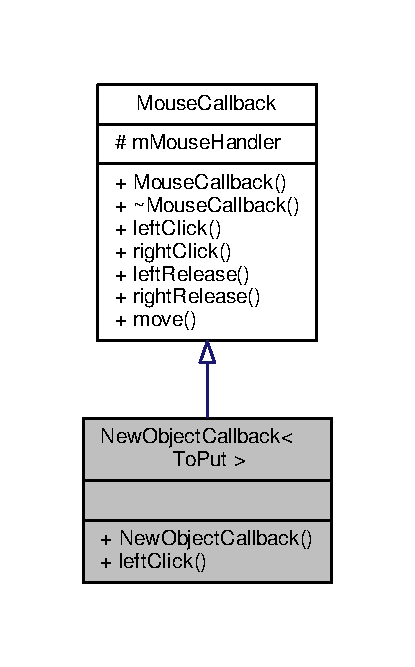
\includegraphics[width=199pt]{classNewObjectCallback__inherit__graph}
\end{center}
\end{figure}


Collaboration diagram for New\+Object\+Callback$<$ To\+Put $>$\+:\nopagebreak
\begin{figure}[H]
\begin{center}
\leavevmode
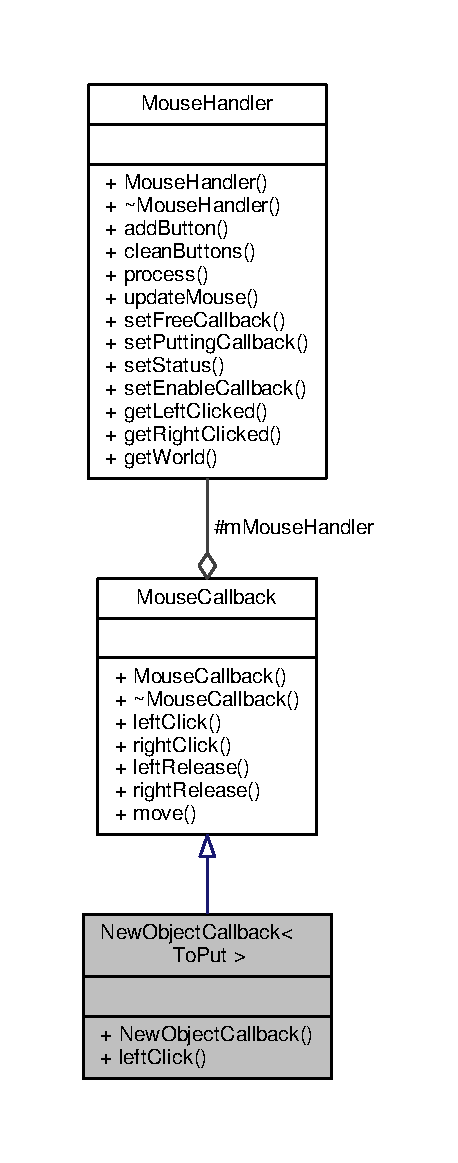
\includegraphics[height=550pt]{classNewObjectCallback__coll__graph}
\end{center}
\end{figure}
\subsection*{Public Member Functions}
\begin{DoxyCompactItemize}
\item 
\hyperlink{classNewObjectCallback_ad84d5f43925125319ea4f11833979e13}{New\+Object\+Callback} (\hyperlink{classMouseHandler}{Mouse\+Handler} $\ast$\+\_\+handler)
\item 
void \hyperlink{classNewObjectCallback_af13d7431504377e66175b9ef9ae3e6fc}{left\+Click} (float x, float y) override
\end{DoxyCompactItemize}
\subsection*{Additional Inherited Members}


\subsection{Constructor \& Destructor Documentation}
\hypertarget{classNewObjectCallback_ad84d5f43925125319ea4f11833979e13}{}\index{New\+Object\+Callback@{New\+Object\+Callback}!New\+Object\+Callback@{New\+Object\+Callback}}
\index{New\+Object\+Callback@{New\+Object\+Callback}!New\+Object\+Callback@{New\+Object\+Callback}}
\subsubsection[{New\+Object\+Callback}]{\setlength{\rightskip}{0pt plus 5cm}template$<$class To\+Put $>$ {\bf New\+Object\+Callback}$<$ To\+Put $>$\+::{\bf New\+Object\+Callback} (
\begin{DoxyParamCaption}
\item[{{\bf Mouse\+Handler} $\ast$}]{\+\_\+handler}
\end{DoxyParamCaption}
)\hspace{0.3cm}{\ttfamily [inline]}}\label{classNewObjectCallback_ad84d5f43925125319ea4f11833979e13}


\subsection{Member Function Documentation}
\hypertarget{classNewObjectCallback_af13d7431504377e66175b9ef9ae3e6fc}{}\index{New\+Object\+Callback@{New\+Object\+Callback}!left\+Click@{left\+Click}}
\index{left\+Click@{left\+Click}!New\+Object\+Callback@{New\+Object\+Callback}}
\subsubsection[{left\+Click}]{\setlength{\rightskip}{0pt plus 5cm}template$<$class To\+Put $>$ void {\bf New\+Object\+Callback}$<$ To\+Put $>$\+::left\+Click (
\begin{DoxyParamCaption}
\item[{float}]{x, }
\item[{float}]{y}
\end{DoxyParamCaption}
)\hspace{0.3cm}{\ttfamily [inline]}, {\ttfamily [override]}, {\ttfamily [virtual]}}\label{classNewObjectCallback_af13d7431504377e66175b9ef9ae3e6fc}


Reimplemented from \hyperlink{classMouseCallback_a5ae88358471f1b48e3f6a730aaf0ba13}{Mouse\+Callback}.



The documentation for this class was generated from the following file\+:\begin{DoxyCompactItemize}
\item 
\hyperlink{mousecallback_8h}{mousecallback.\+h}\end{DoxyCompactItemize}

\hypertarget{classParticleSystem}{}\section{Particle\+System Class Reference}
\label{classParticleSystem}\index{Particle\+System@{Particle\+System}}


Base class of all particle systems.  




{\ttfamily \#include $<$matter.\+h$>$}



Inheritance diagram for Particle\+System\+:
\nopagebreak
\begin{figure}[H]
\begin{center}
\leavevmode
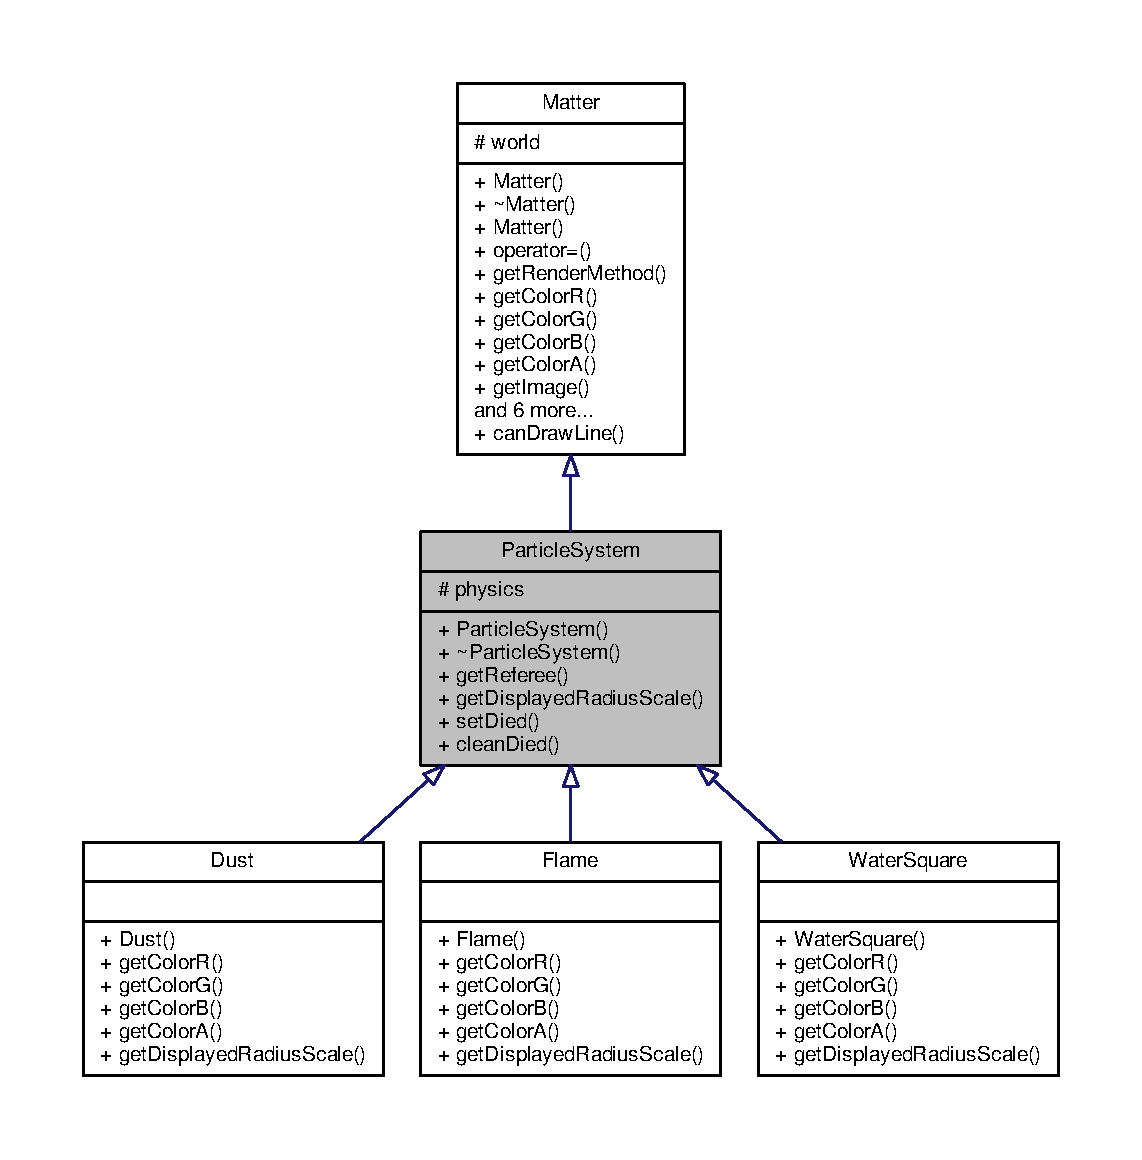
\includegraphics[width=350pt]{classParticleSystem__inherit__graph}
\end{center}
\end{figure}


Collaboration diagram for Particle\+System\+:
\nopagebreak
\begin{figure}[H]
\begin{center}
\leavevmode
\includegraphics[height=550pt]{classParticleSystem__coll__graph}
\end{center}
\end{figure}
\subsection*{Public Member Functions}
\begin{DoxyCompactItemize}
\item 
\hyperlink{classParticleSystem_abbb50f9bc17e323468e70a2e99fe8a10}{Particle\+System} (\hyperlink{classWorld}{World} $\ast$\+\_\+world, const b2\+Particle\+System\+Def \&system\+Def, const std\+::vector$<$ b2\+Particle\+Group\+Def $>$ \&group\+Defs) noexcept
\begin{DoxyCompactList}\small\item\em N\+O\+T\+I\+C\+E\+: Pointer to b2\+Shape in group\+Defs will be deleted. \end{DoxyCompactList}\item 
virtual \hyperlink{classParticleSystem_a257c75371728135e1209f0549d8eeb15}{$\sim$\+Particle\+System} () noexcept
\item 
b2\+Particle\+System $\ast$ \hyperlink{classParticleSystem_a7a3ebd9985d271a93fedcdb3894ebb8b}{get\+Referee} () const 
\item 
virtual float \hyperlink{classParticleSystem_a5b3bcfbc82de5d335f55173b049da517}{get\+Displayed\+Radius\+Scale} () const =0
\begin{DoxyCompactList}\small\item\em displayed radius = ? $\ast$ physics radius \end{DoxyCompactList}\end{DoxyCompactItemize}
\subsection*{Static Public Member Functions}
\begin{DoxyCompactItemize}
\item 
static void \hyperlink{classParticleSystem_a95379b5f53c63735dc9c7f76ac47ba98}{set\+Died} (\hyperlink{classParticleSystem}{Particle\+System} $\ast$system)
\begin{DoxyCompactList}\small\item\em Set to delete it in next round. \end{DoxyCompactList}\item 
static void \hyperlink{classParticleSystem_a38a1e26b5200ce585e17c71553273882}{clean\+Died} ()
\begin{DoxyCompactList}\small\item\em Clean all died. \end{DoxyCompactList}\end{DoxyCompactItemize}
\subsection*{Protected Attributes}
\begin{DoxyCompactItemize}
\item 
b2\+Particle\+System $\ast$ \hyperlink{classParticleSystem_a899787ecc1f14a30cd903a884ec7575e}{physics}
\end{DoxyCompactItemize}
\subsection*{Static Private Attributes}
\begin{DoxyCompactItemize}
\item 
static std\+::list$<$ \hyperlink{classParticleSystem}{Particle\+System} $\ast$ $>$ \hyperlink{classParticleSystem_a58e021cbc8991ca7191d36d7adcb3167}{died}
\end{DoxyCompactItemize}
\subsection*{Additional Inherited Members}


\subsection{Detailed Description}
Base class of all particle systems. 

\subsection{Constructor \& Destructor Documentation}
\hypertarget{classParticleSystem_abbb50f9bc17e323468e70a2e99fe8a10}{}\index{Particle\+System@{Particle\+System}!Particle\+System@{Particle\+System}}
\index{Particle\+System@{Particle\+System}!Particle\+System@{Particle\+System}}
\subsubsection[{Particle\+System}]{\setlength{\rightskip}{0pt plus 5cm}Particle\+System\+::\+Particle\+System (
\begin{DoxyParamCaption}
\item[{{\bf World} $\ast$}]{\+\_\+world, }
\item[{const b2\+Particle\+System\+Def \&}]{system\+Def, }
\item[{const std\+::vector$<$ b2\+Particle\+Group\+Def $>$ \&}]{group\+Defs}
\end{DoxyParamCaption}
)\hspace{0.3cm}{\ttfamily [noexcept]}}\label{classParticleSystem_abbb50f9bc17e323468e70a2e99fe8a10}


N\+O\+T\+I\+C\+E\+: Pointer to b2\+Shape in group\+Defs will be deleted. 

\hypertarget{classParticleSystem_a257c75371728135e1209f0549d8eeb15}{}\index{Particle\+System@{Particle\+System}!````~Particle\+System@{$\sim$\+Particle\+System}}
\index{````~Particle\+System@{$\sim$\+Particle\+System}!Particle\+System@{Particle\+System}}
\subsubsection[{$\sim$\+Particle\+System}]{\setlength{\rightskip}{0pt plus 5cm}Particle\+System\+::$\sim$\+Particle\+System (
\begin{DoxyParamCaption}
{}
\end{DoxyParamCaption}
)\hspace{0.3cm}{\ttfamily [virtual]}, {\ttfamily [noexcept]}}\label{classParticleSystem_a257c75371728135e1209f0549d8eeb15}


\subsection{Member Function Documentation}
\hypertarget{classParticleSystem_a38a1e26b5200ce585e17c71553273882}{}\index{Particle\+System@{Particle\+System}!clean\+Died@{clean\+Died}}
\index{clean\+Died@{clean\+Died}!Particle\+System@{Particle\+System}}
\subsubsection[{clean\+Died}]{\setlength{\rightskip}{0pt plus 5cm}void Particle\+System\+::clean\+Died (
\begin{DoxyParamCaption}
{}
\end{DoxyParamCaption}
)\hspace{0.3cm}{\ttfamily [static]}}\label{classParticleSystem_a38a1e26b5200ce585e17c71553273882}


Clean all died. 

\hypertarget{classParticleSystem_a5b3bcfbc82de5d335f55173b049da517}{}\index{Particle\+System@{Particle\+System}!get\+Displayed\+Radius\+Scale@{get\+Displayed\+Radius\+Scale}}
\index{get\+Displayed\+Radius\+Scale@{get\+Displayed\+Radius\+Scale}!Particle\+System@{Particle\+System}}
\subsubsection[{get\+Displayed\+Radius\+Scale}]{\setlength{\rightskip}{0pt plus 5cm}virtual float Particle\+System\+::get\+Displayed\+Radius\+Scale (
\begin{DoxyParamCaption}
{}
\end{DoxyParamCaption}
) const\hspace{0.3cm}{\ttfamily [pure virtual]}}\label{classParticleSystem_a5b3bcfbc82de5d335f55173b049da517}


displayed radius = ? $\ast$ physics radius 



Implemented in \hyperlink{classFlame_a472dc6269e6e13b4628abd2392726fd8}{Flame}, \hyperlink{classDust_a6e96475d0b48ffcfb443c014ad369276}{Dust}, and \hyperlink{classWaterSquare_aefb21ab0a4f52f3fbd998d2c7e4feed4}{Water\+Square}.

\hypertarget{classParticleSystem_a7a3ebd9985d271a93fedcdb3894ebb8b}{}\index{Particle\+System@{Particle\+System}!get\+Referee@{get\+Referee}}
\index{get\+Referee@{get\+Referee}!Particle\+System@{Particle\+System}}
\subsubsection[{get\+Referee}]{\setlength{\rightskip}{0pt plus 5cm}b2\+Particle\+System$\ast$ Particle\+System\+::get\+Referee (
\begin{DoxyParamCaption}
{}
\end{DoxyParamCaption}
) const\hspace{0.3cm}{\ttfamily [inline]}}\label{classParticleSystem_a7a3ebd9985d271a93fedcdb3894ebb8b}
\hypertarget{classParticleSystem_a95379b5f53c63735dc9c7f76ac47ba98}{}\index{Particle\+System@{Particle\+System}!set\+Died@{set\+Died}}
\index{set\+Died@{set\+Died}!Particle\+System@{Particle\+System}}
\subsubsection[{set\+Died}]{\setlength{\rightskip}{0pt plus 5cm}static void Particle\+System\+::set\+Died (
\begin{DoxyParamCaption}
\item[{{\bf Particle\+System} $\ast$}]{system}
\end{DoxyParamCaption}
)\hspace{0.3cm}{\ttfamily [inline]}, {\ttfamily [static]}}\label{classParticleSystem_a95379b5f53c63735dc9c7f76ac47ba98}


Set to delete it in next round. 



\subsection{Member Data Documentation}
\hypertarget{classParticleSystem_a58e021cbc8991ca7191d36d7adcb3167}{}\index{Particle\+System@{Particle\+System}!died@{died}}
\index{died@{died}!Particle\+System@{Particle\+System}}
\subsubsection[{died}]{\setlength{\rightskip}{0pt plus 5cm}std\+::list$<$ {\bf Particle\+System} $\ast$ $>$ Particle\+System\+::died\hspace{0.3cm}{\ttfamily [static]}, {\ttfamily [private]}}\label{classParticleSystem_a58e021cbc8991ca7191d36d7adcb3167}
\hypertarget{classParticleSystem_a899787ecc1f14a30cd903a884ec7575e}{}\index{Particle\+System@{Particle\+System}!physics@{physics}}
\index{physics@{physics}!Particle\+System@{Particle\+System}}
\subsubsection[{physics}]{\setlength{\rightskip}{0pt plus 5cm}b2\+Particle\+System$\ast$ Particle\+System\+::physics\hspace{0.3cm}{\ttfamily [protected]}}\label{classParticleSystem_a899787ecc1f14a30cd903a884ec7575e}


The documentation for this class was generated from the following files\+:\begin{DoxyCompactItemize}
\item 
\hyperlink{matter_8h}{matter.\+h}\item 
\hyperlink{matter_8cpp}{matter.\+cpp}\end{DoxyCompactItemize}

\hypertarget{classRender_1_1PolygonRenderer}{}\section{Render\+:\+:Polygon\+Renderer Class Reference}
\label{classRender_1_1PolygonRenderer}\index{Render\+::\+Polygon\+Renderer@{Render\+::\+Polygon\+Renderer}}


Inheritance diagram for Render\+:\+:Polygon\+Renderer\+:
\nopagebreak
\begin{figure}[H]
\begin{center}
\leavevmode
\includegraphics[width=209pt]{classRender_1_1PolygonRenderer__inherit__graph}
\end{center}
\end{figure}


Collaboration diagram for Render\+:\+:Polygon\+Renderer\+:
\nopagebreak
\begin{figure}[H]
\begin{center}
\leavevmode
\includegraphics[height=550pt]{classRender_1_1PolygonRenderer__coll__graph}
\end{center}
\end{figure}
\subsection*{Public Member Functions}
\begin{DoxyCompactItemize}
\item 
\hyperlink{classRender_1_1PolygonRenderer_a838a3a8cf080315b7524b0b55dfcf9bc}{Polygon\+Renderer} (const b2\+Body $\ast$\+\_\+b, const b2\+Fixture $\ast$\+\_\+f, float \+\_\+scale) noexcept
\item 
void \hyperlink{classRender_1_1PolygonRenderer_af3e5d487898b3f7e0da7edcfc59967ba}{draw\+Edge} () noexceptoverride
\item 
void \hyperlink{classRender_1_1PolygonRenderer_aec84603818d0ce8ba1805c4828505578}{draw\+Main} () noexceptoverride
\item 
void \hyperlink{classRender_1_1PolygonRenderer_ade951f9c8f1034823aecab89fe06aa9c}{draw\+Alert} () noexceptoverride
\end{DoxyCompactItemize}
\subsection*{Private Attributes}
\begin{DoxyCompactItemize}
\item 
std\+::vector$<$ b2\+Vec2 $>$ \hyperlink{classRender_1_1PolygonRenderer_ab4986f5dd990859f59e9b37b52dd352d}{vert}
\item 
std\+::vector$<$ b2\+Vec2 $>$ \hyperlink{classRender_1_1PolygonRenderer_ad7a634f5ab472fc121698f8e5a288f31}{local\+Vert}
\item 
b2\+Vec2 \hyperlink{classRender_1_1PolygonRenderer_a9f2dc2e4bff2308cb37b7573307cb4c5}{local\+Center}
\end{DoxyCompactItemize}
\subsection*{Additional Inherited Members}


\subsection{Constructor \& Destructor Documentation}
\hypertarget{classRender_1_1PolygonRenderer_a838a3a8cf080315b7524b0b55dfcf9bc}{}\index{Render\+::\+Polygon\+Renderer@{Render\+::\+Polygon\+Renderer}!Polygon\+Renderer@{Polygon\+Renderer}}
\index{Polygon\+Renderer@{Polygon\+Renderer}!Render\+::\+Polygon\+Renderer@{Render\+::\+Polygon\+Renderer}}
\subsubsection[{Polygon\+Renderer}]{\setlength{\rightskip}{0pt plus 5cm}Render\+::\+Polygon\+Renderer\+::\+Polygon\+Renderer (
\begin{DoxyParamCaption}
\item[{const b2\+Body $\ast$}]{\+\_\+b, }
\item[{const b2\+Fixture $\ast$}]{\+\_\+f, }
\item[{float}]{\+\_\+scale}
\end{DoxyParamCaption}
)\hspace{0.3cm}{\ttfamily [noexcept]}}\label{classRender_1_1PolygonRenderer_a838a3a8cf080315b7524b0b55dfcf9bc}


\subsection{Member Function Documentation}
\hypertarget{classRender_1_1PolygonRenderer_ade951f9c8f1034823aecab89fe06aa9c}{}\index{Render\+::\+Polygon\+Renderer@{Render\+::\+Polygon\+Renderer}!draw\+Alert@{draw\+Alert}}
\index{draw\+Alert@{draw\+Alert}!Render\+::\+Polygon\+Renderer@{Render\+::\+Polygon\+Renderer}}
\subsubsection[{draw\+Alert}]{\setlength{\rightskip}{0pt plus 5cm}void Render\+::\+Polygon\+Renderer\+::draw\+Alert (
\begin{DoxyParamCaption}
{}
\end{DoxyParamCaption}
)\hspace{0.3cm}{\ttfamily [override]}, {\ttfamily [virtual]}, {\ttfamily [noexcept]}}\label{classRender_1_1PolygonRenderer_ade951f9c8f1034823aecab89fe06aa9c}


Reimplemented from \hyperlink{classRender_1_1FixtureRenderer_a3208fef7547ef2f61d68ddfd3ceb05da}{Render\+::\+Fixture\+Renderer}.

\hypertarget{classRender_1_1PolygonRenderer_af3e5d487898b3f7e0da7edcfc59967ba}{}\index{Render\+::\+Polygon\+Renderer@{Render\+::\+Polygon\+Renderer}!draw\+Edge@{draw\+Edge}}
\index{draw\+Edge@{draw\+Edge}!Render\+::\+Polygon\+Renderer@{Render\+::\+Polygon\+Renderer}}
\subsubsection[{draw\+Edge}]{\setlength{\rightskip}{0pt plus 5cm}void Render\+::\+Polygon\+Renderer\+::draw\+Edge (
\begin{DoxyParamCaption}
{}
\end{DoxyParamCaption}
)\hspace{0.3cm}{\ttfamily [override]}, {\ttfamily [virtual]}, {\ttfamily [noexcept]}}\label{classRender_1_1PolygonRenderer_af3e5d487898b3f7e0da7edcfc59967ba}


Reimplemented from \hyperlink{classRender_1_1FixtureRenderer_af0b5bfc5af5a2bb4a80eb7afc7e1398f}{Render\+::\+Fixture\+Renderer}.

\hypertarget{classRender_1_1PolygonRenderer_aec84603818d0ce8ba1805c4828505578}{}\index{Render\+::\+Polygon\+Renderer@{Render\+::\+Polygon\+Renderer}!draw\+Main@{draw\+Main}}
\index{draw\+Main@{draw\+Main}!Render\+::\+Polygon\+Renderer@{Render\+::\+Polygon\+Renderer}}
\subsubsection[{draw\+Main}]{\setlength{\rightskip}{0pt plus 5cm}void Render\+::\+Polygon\+Renderer\+::draw\+Main (
\begin{DoxyParamCaption}
{}
\end{DoxyParamCaption}
)\hspace{0.3cm}{\ttfamily [override]}, {\ttfamily [virtual]}, {\ttfamily [noexcept]}}\label{classRender_1_1PolygonRenderer_aec84603818d0ce8ba1805c4828505578}


Reimplemented from \hyperlink{classRender_1_1FixtureRenderer_a20f23477aa8cc646f2d18b0165666e3b}{Render\+::\+Fixture\+Renderer}.



\subsection{Member Data Documentation}
\hypertarget{classRender_1_1PolygonRenderer_a9f2dc2e4bff2308cb37b7573307cb4c5}{}\index{Render\+::\+Polygon\+Renderer@{Render\+::\+Polygon\+Renderer}!local\+Center@{local\+Center}}
\index{local\+Center@{local\+Center}!Render\+::\+Polygon\+Renderer@{Render\+::\+Polygon\+Renderer}}
\subsubsection[{local\+Center}]{\setlength{\rightskip}{0pt plus 5cm}b2\+Vec2 Render\+::\+Polygon\+Renderer\+::local\+Center\hspace{0.3cm}{\ttfamily [private]}}\label{classRender_1_1PolygonRenderer_a9f2dc2e4bff2308cb37b7573307cb4c5}
\hypertarget{classRender_1_1PolygonRenderer_ad7a634f5ab472fc121698f8e5a288f31}{}\index{Render\+::\+Polygon\+Renderer@{Render\+::\+Polygon\+Renderer}!local\+Vert@{local\+Vert}}
\index{local\+Vert@{local\+Vert}!Render\+::\+Polygon\+Renderer@{Render\+::\+Polygon\+Renderer}}
\subsubsection[{local\+Vert}]{\setlength{\rightskip}{0pt plus 5cm}std\+::vector$<$b2\+Vec2$>$ Render\+::\+Polygon\+Renderer\+::local\+Vert\hspace{0.3cm}{\ttfamily [private]}}\label{classRender_1_1PolygonRenderer_ad7a634f5ab472fc121698f8e5a288f31}
\hypertarget{classRender_1_1PolygonRenderer_ab4986f5dd990859f59e9b37b52dd352d}{}\index{Render\+::\+Polygon\+Renderer@{Render\+::\+Polygon\+Renderer}!vert@{vert}}
\index{vert@{vert}!Render\+::\+Polygon\+Renderer@{Render\+::\+Polygon\+Renderer}}
\subsubsection[{vert}]{\setlength{\rightskip}{0pt plus 5cm}std\+::vector$<$b2\+Vec2$>$ Render\+::\+Polygon\+Renderer\+::vert\hspace{0.3cm}{\ttfamily [private]}}\label{classRender_1_1PolygonRenderer_ab4986f5dd990859f59e9b37b52dd352d}


The documentation for this class was generated from the following files\+:\begin{DoxyCompactItemize}
\item 
\hyperlink{render_8h}{render.\+h}\item 
\hyperlink{render_8cpp}{render.\+cpp}\end{DoxyCompactItemize}

\hypertarget{classPuttingCallback}{}\section{Putting\+Callback$<$ To\+Put $>$ Class Template Reference}
\label{classPuttingCallback}\index{Putting\+Callback$<$ To\+Put $>$@{Putting\+Callback$<$ To\+Put $>$}}


Callbacks of putting normal things that ! can\+Draw\+Line()  




{\ttfamily \#include $<$mousecallback.\+h$>$}



Inheritance diagram for Putting\+Callback$<$ To\+Put $>$\+:\nopagebreak
\begin{figure}[H]
\begin{center}
\leavevmode
\includegraphics[width=210pt]{classPuttingCallback__inherit__graph}
\end{center}
\end{figure}


Collaboration diagram for Putting\+Callback$<$ To\+Put $>$\+:\nopagebreak
\begin{figure}[H]
\begin{center}
\leavevmode
\includegraphics[height=550pt]{classPuttingCallback__coll__graph}
\end{center}
\end{figure}
\subsection*{Public Member Functions}
\begin{DoxyCompactItemize}
\item 
\hyperlink{classPuttingCallback_abd83a02e857748d0ec88e30fcf08eb5e}{Putting\+Callback} (\hyperlink{classMouseHandler}{Mouse\+Handler} $\ast$\+\_\+handler, float x, float y)
\item 
void \hyperlink{classPuttingCallback_a95d8a7c64a5c1967982c0e6ef0d36969}{left\+Click} (float x, float y) override
\item 
void \hyperlink{classPuttingCallback_a9be086c4e02d2d9911876bbe17840f10}{right\+Click} (float x, float y) override
\item 
void \hyperlink{classPuttingCallback_a9d82e38a9f790cbfeb4bf24f81110deb}{move} (float x, float y) override
\end{DoxyCompactItemize}
\subsection*{Additional Inherited Members}


\subsection{Detailed Description}
\subsubsection*{template$<$class To\+Put$>$class Putting\+Callback$<$ To\+Put $>$}

Callbacks of putting normal things that ! can\+Draw\+Line() 

\subsection{Constructor \& Destructor Documentation}
\hypertarget{classPuttingCallback_abd83a02e857748d0ec88e30fcf08eb5e}{}\index{Putting\+Callback@{Putting\+Callback}!Putting\+Callback@{Putting\+Callback}}
\index{Putting\+Callback@{Putting\+Callback}!Putting\+Callback@{Putting\+Callback}}
\subsubsection[{Putting\+Callback}]{\setlength{\rightskip}{0pt plus 5cm}template$<$class To\+Put$>$ {\bf Putting\+Callback}$<$ To\+Put $>$\+::{\bf Putting\+Callback} (
\begin{DoxyParamCaption}
\item[{{\bf Mouse\+Handler} $\ast$}]{\+\_\+handler, }
\item[{float}]{x, }
\item[{float}]{y}
\end{DoxyParamCaption}
)\hspace{0.3cm}{\ttfamily [inline]}}\label{classPuttingCallback_abd83a02e857748d0ec88e30fcf08eb5e}


\subsection{Member Function Documentation}
\hypertarget{classPuttingCallback_a95d8a7c64a5c1967982c0e6ef0d36969}{}\index{Putting\+Callback@{Putting\+Callback}!left\+Click@{left\+Click}}
\index{left\+Click@{left\+Click}!Putting\+Callback@{Putting\+Callback}}
\subsubsection[{left\+Click}]{\setlength{\rightskip}{0pt plus 5cm}template$<$class To\+Put$>$ void {\bf Putting\+Callback}$<$ To\+Put $>$\+::left\+Click (
\begin{DoxyParamCaption}
\item[{float}]{x, }
\item[{float}]{y}
\end{DoxyParamCaption}
)\hspace{0.3cm}{\ttfamily [inline]}, {\ttfamily [override]}, {\ttfamily [virtual]}}\label{classPuttingCallback_a95d8a7c64a5c1967982c0e6ef0d36969}


Reimplemented from \hyperlink{classMouseCallback_a5ae88358471f1b48e3f6a730aaf0ba13}{Mouse\+Callback}.

\hypertarget{classPuttingCallback_a9d82e38a9f790cbfeb4bf24f81110deb}{}\index{Putting\+Callback@{Putting\+Callback}!move@{move}}
\index{move@{move}!Putting\+Callback@{Putting\+Callback}}
\subsubsection[{move}]{\setlength{\rightskip}{0pt plus 5cm}template$<$class To\+Put$>$ void {\bf Putting\+Callback}$<$ To\+Put $>$\+::move (
\begin{DoxyParamCaption}
\item[{float}]{x, }
\item[{float}]{y}
\end{DoxyParamCaption}
)\hspace{0.3cm}{\ttfamily [inline]}, {\ttfamily [override]}, {\ttfamily [virtual]}}\label{classPuttingCallback_a9d82e38a9f790cbfeb4bf24f81110deb}


Reimplemented from \hyperlink{classMouseCallback_a9a667f1501597e44af0e0d9f1dfcbd6a}{Mouse\+Callback}.

\hypertarget{classPuttingCallback_a9be086c4e02d2d9911876bbe17840f10}{}\index{Putting\+Callback@{Putting\+Callback}!right\+Click@{right\+Click}}
\index{right\+Click@{right\+Click}!Putting\+Callback@{Putting\+Callback}}
\subsubsection[{right\+Click}]{\setlength{\rightskip}{0pt plus 5cm}template$<$class To\+Put$>$ void {\bf Putting\+Callback}$<$ To\+Put $>$\+::right\+Click (
\begin{DoxyParamCaption}
\item[{float}]{x, }
\item[{float}]{y}
\end{DoxyParamCaption}
)\hspace{0.3cm}{\ttfamily [inline]}, {\ttfamily [override]}, {\ttfamily [virtual]}}\label{classPuttingCallback_a9be086c4e02d2d9911876bbe17840f10}


Reimplemented from \hyperlink{classMouseCallback_aa4a0c30b50b48972d0a48b9aff6344c5}{Mouse\+Callback}.



The documentation for this class was generated from the following file\+:\begin{DoxyCompactItemize}
\item 
\hyperlink{mousecallback_8h}{mousecallback.\+h}\end{DoxyCompactItemize}

\hypertarget{classPuttingLineCallback}{}\section{Putting\+Line\+Callback$<$ To\+Put $>$ Class Template Reference}
\label{classPuttingLineCallback}\index{Putting\+Line\+Callback$<$ To\+Put $>$@{Putting\+Line\+Callback$<$ To\+Put $>$}}


Putting rigids with can\+Draw\+Line()  




{\ttfamily \#include $<$mousecallback.\+h$>$}



Inheritance diagram for Putting\+Line\+Callback$<$ To\+Put $>$\+:
\nopagebreak
\begin{figure}[H]
\begin{center}
\leavevmode
\includegraphics[width=205pt]{classPuttingLineCallback__inherit__graph}
\end{center}
\end{figure}


Collaboration diagram for Putting\+Line\+Callback$<$ To\+Put $>$\+:
\nopagebreak
\begin{figure}[H]
\begin{center}
\leavevmode
\includegraphics[height=550pt]{classPuttingLineCallback__coll__graph}
\end{center}
\end{figure}
\subsection*{Public Member Functions}
\begin{DoxyCompactItemize}
\item 
\hyperlink{classPuttingLineCallback_a7bf8b242abd061bbe1724f837c379ea2}{Putting\+Line\+Callback} (\hyperlink{classMouseHandler}{Mouse\+Handler} $\ast$\+\_\+handler, float x, float y)
\item 
\hyperlink{classPuttingLineCallback_a3835ab594c3a188eae9d8beff4802e5f}{$\sim$\+Putting\+Line\+Callback} ()
\item 
void \hyperlink{classPuttingLineCallback_a5a4c924a90e4b2ec3a359ae1f958d168}{left\+Click} (float x, float y) override
\item 
void \hyperlink{classPuttingLineCallback_a87d406ea7eb6fb24f2777b9bb8032a5a}{right\+Click} (float x, float y) override
\item 
void \hyperlink{classPuttingLineCallback_abc6f400a8e408faa4ae2ebbc8eef8dca}{move} (float x, float y) override
\end{DoxyCompactItemize}
\subsection*{Private Attributes}
\begin{DoxyCompactItemize}
\item 
float \hyperlink{classPuttingLineCallback_af7ede0099cc6ee2eb5ccf3cda667c711}{sx}
\item 
float \hyperlink{classPuttingLineCallback_a92d6e9d843c9022499da9029220b78bd}{sy}
\item 
bool \hyperlink{classPuttingLineCallback_aa2bcbb0e5a6132e4bb8b87684bff26c2}{drawing}
\end{DoxyCompactItemize}
\subsection*{Additional Inherited Members}


\subsection{Detailed Description}
\subsubsection*{template$<$class To\+Put$>$class Putting\+Line\+Callback$<$ To\+Put $>$}

Putting rigids with can\+Draw\+Line() 

\subsection{Constructor \& Destructor Documentation}
\hypertarget{classPuttingLineCallback_a7bf8b242abd061bbe1724f837c379ea2}{}\index{Putting\+Line\+Callback@{Putting\+Line\+Callback}!Putting\+Line\+Callback@{Putting\+Line\+Callback}}
\index{Putting\+Line\+Callback@{Putting\+Line\+Callback}!Putting\+Line\+Callback@{Putting\+Line\+Callback}}
\subsubsection[{Putting\+Line\+Callback}]{\setlength{\rightskip}{0pt plus 5cm}template$<$class To\+Put$>$ {\bf Putting\+Line\+Callback}$<$ To\+Put $>$\+::{\bf Putting\+Line\+Callback} (
\begin{DoxyParamCaption}
\item[{{\bf Mouse\+Handler} $\ast$}]{\+\_\+handler, }
\item[{float}]{x, }
\item[{float}]{y}
\end{DoxyParamCaption}
)\hspace{0.3cm}{\ttfamily [inline]}}\label{classPuttingLineCallback_a7bf8b242abd061bbe1724f837c379ea2}
\hypertarget{classPuttingLineCallback_a3835ab594c3a188eae9d8beff4802e5f}{}\index{Putting\+Line\+Callback@{Putting\+Line\+Callback}!````~Putting\+Line\+Callback@{$\sim$\+Putting\+Line\+Callback}}
\index{````~Putting\+Line\+Callback@{$\sim$\+Putting\+Line\+Callback}!Putting\+Line\+Callback@{Putting\+Line\+Callback}}
\subsubsection[{$\sim$\+Putting\+Line\+Callback}]{\setlength{\rightskip}{0pt plus 5cm}template$<$class To\+Put$>$ {\bf Putting\+Line\+Callback}$<$ To\+Put $>$\+::$\sim${\bf Putting\+Line\+Callback} (
\begin{DoxyParamCaption}
{}
\end{DoxyParamCaption}
)\hspace{0.3cm}{\ttfamily [inline]}}\label{classPuttingLineCallback_a3835ab594c3a188eae9d8beff4802e5f}


\subsection{Member Function Documentation}
\hypertarget{classPuttingLineCallback_a5a4c924a90e4b2ec3a359ae1f958d168}{}\index{Putting\+Line\+Callback@{Putting\+Line\+Callback}!left\+Click@{left\+Click}}
\index{left\+Click@{left\+Click}!Putting\+Line\+Callback@{Putting\+Line\+Callback}}
\subsubsection[{left\+Click}]{\setlength{\rightskip}{0pt plus 5cm}template$<$class To\+Put$>$ void {\bf Putting\+Line\+Callback}$<$ To\+Put $>$\+::left\+Click (
\begin{DoxyParamCaption}
\item[{float}]{x, }
\item[{float}]{y}
\end{DoxyParamCaption}
)\hspace{0.3cm}{\ttfamily [inline]}, {\ttfamily [override]}, {\ttfamily [virtual]}}\label{classPuttingLineCallback_a5a4c924a90e4b2ec3a359ae1f958d168}


Reimplemented from \hyperlink{classMouseCallback_a5ae88358471f1b48e3f6a730aaf0ba13}{Mouse\+Callback}.

\hypertarget{classPuttingLineCallback_abc6f400a8e408faa4ae2ebbc8eef8dca}{}\index{Putting\+Line\+Callback@{Putting\+Line\+Callback}!move@{move}}
\index{move@{move}!Putting\+Line\+Callback@{Putting\+Line\+Callback}}
\subsubsection[{move}]{\setlength{\rightskip}{0pt plus 5cm}template$<$class To\+Put$>$ void {\bf Putting\+Line\+Callback}$<$ To\+Put $>$\+::move (
\begin{DoxyParamCaption}
\item[{float}]{x, }
\item[{float}]{y}
\end{DoxyParamCaption}
)\hspace{0.3cm}{\ttfamily [inline]}, {\ttfamily [override]}, {\ttfamily [virtual]}}\label{classPuttingLineCallback_abc6f400a8e408faa4ae2ebbc8eef8dca}


Reimplemented from \hyperlink{classMouseCallback_a9a667f1501597e44af0e0d9f1dfcbd6a}{Mouse\+Callback}.

\hypertarget{classPuttingLineCallback_a87d406ea7eb6fb24f2777b9bb8032a5a}{}\index{Putting\+Line\+Callback@{Putting\+Line\+Callback}!right\+Click@{right\+Click}}
\index{right\+Click@{right\+Click}!Putting\+Line\+Callback@{Putting\+Line\+Callback}}
\subsubsection[{right\+Click}]{\setlength{\rightskip}{0pt plus 5cm}template$<$class To\+Put$>$ void {\bf Putting\+Line\+Callback}$<$ To\+Put $>$\+::right\+Click (
\begin{DoxyParamCaption}
\item[{float}]{x, }
\item[{float}]{y}
\end{DoxyParamCaption}
)\hspace{0.3cm}{\ttfamily [inline]}, {\ttfamily [override]}, {\ttfamily [virtual]}}\label{classPuttingLineCallback_a87d406ea7eb6fb24f2777b9bb8032a5a}


Reimplemented from \hyperlink{classMouseCallback_aa4a0c30b50b48972d0a48b9aff6344c5}{Mouse\+Callback}.



\subsection{Member Data Documentation}
\hypertarget{classPuttingLineCallback_aa2bcbb0e5a6132e4bb8b87684bff26c2}{}\index{Putting\+Line\+Callback@{Putting\+Line\+Callback}!drawing@{drawing}}
\index{drawing@{drawing}!Putting\+Line\+Callback@{Putting\+Line\+Callback}}
\subsubsection[{drawing}]{\setlength{\rightskip}{0pt plus 5cm}template$<$class To\+Put$>$ bool {\bf Putting\+Line\+Callback}$<$ To\+Put $>$\+::drawing\hspace{0.3cm}{\ttfamily [private]}}\label{classPuttingLineCallback_aa2bcbb0e5a6132e4bb8b87684bff26c2}
\hypertarget{classPuttingLineCallback_af7ede0099cc6ee2eb5ccf3cda667c711}{}\index{Putting\+Line\+Callback@{Putting\+Line\+Callback}!sx@{sx}}
\index{sx@{sx}!Putting\+Line\+Callback@{Putting\+Line\+Callback}}
\subsubsection[{sx}]{\setlength{\rightskip}{0pt plus 5cm}template$<$class To\+Put$>$ float {\bf Putting\+Line\+Callback}$<$ To\+Put $>$\+::sx\hspace{0.3cm}{\ttfamily [private]}}\label{classPuttingLineCallback_af7ede0099cc6ee2eb5ccf3cda667c711}
\hypertarget{classPuttingLineCallback_a92d6e9d843c9022499da9029220b78bd}{}\index{Putting\+Line\+Callback@{Putting\+Line\+Callback}!sy@{sy}}
\index{sy@{sy}!Putting\+Line\+Callback@{Putting\+Line\+Callback}}
\subsubsection[{sy}]{\setlength{\rightskip}{0pt plus 5cm}template$<$class To\+Put$>$ float {\bf Putting\+Line\+Callback}$<$ To\+Put $>$\+::sy\hspace{0.3cm}{\ttfamily [private]}}\label{classPuttingLineCallback_a92d6e9d843c9022499da9029220b78bd}


The documentation for this class was generated from the following file\+:\begin{DoxyCompactItemize}
\item 
\hyperlink{mousecallback_8h}{mousecallback.\+h}\end{DoxyCompactItemize}

\hypertarget{classRender}{}\section{Render Class Reference}
\label{classRender}\index{Render@{Render}}


{\ttfamily \#include $<$render.\+h$>$}



Collaboration diagram for Render\+:\nopagebreak
\begin{figure}[H]
\begin{center}
\leavevmode
\includegraphics[width=199pt]{classRender__coll__graph}
\end{center}
\end{figure}
\subsection*{Public Member Functions}
\begin{DoxyCompactItemize}
\item 
\hyperlink{classRender_a9efce92fa87e96980f4e413ee0cb6843}{Render} (const \hyperlink{classRender}{Render} \&)=delete
\item 
\hyperlink{classRender_a6e1a004027eff97cb3dfc9f012dde498}{Render} (\hyperlink{classRender}{Render} \&\&)=delete
\item 
void \hyperlink{classRender_a18f55be699e0bd8d20a5462330d5c9df}{draw\+Rigid} (const b2\+Body $\ast$\hyperlink{image_8h_ab2d05693952610f937e5acb3c4a8fa1b}{b}, float world\+Scale) noexcept
\item 
void \hyperlink{classRender_a14b83adbf9e351b9f11383abeef2ca63}{draw\+Particle\+System} (const b2\+Particle\+System $\ast$s, float world\+Scale) noexcept
\item 
void \hyperlink{classRender_a4f2ee414b80bf5e1e1ffcfe80c33218a}{draw\+Line} (float x1, float y1, float x2, float y2) noexcept
\begin{DoxyCompactList}\small\item\em draw a line from (x1,y1) to (x2,y2) (in world coordinates) \end{DoxyCompactList}\item 
void \hyperlink{classRender_ac30bcc966a9aa9de650a80cbfc600bb1}{draw\+Popup} (const std\+::string \&s, float l, float \hyperlink{image_8h_a62969232668331297e2dca1ae2ddd10d}{r}, float d, float u) noexcept
\begin{DoxyCompactList}\small\item\em draw a popup window with text, and with lower-\/left (l,d) and upper-\/right(r,u) (in world coordinates) \end{DoxyCompactList}\end{DoxyCompactItemize}
\subsection*{Static Public Member Functions}
\begin{DoxyCompactItemize}
\item 
static \hyperlink{classRender}{Render} \& \hyperlink{classRender_add2a1980ba1c0d0bce85943405f87c68}{get\+Instance} ()
\item 
static void \hyperlink{classRender_ae6344724a34c4ec00fc3f9de97a7cdb6}{set\+Window} (const \hyperlink{classWindow}{Window} $\ast$\+\_\+window)
\end{DoxyCompactItemize}


\subsection{Constructor \& Destructor Documentation}
\hypertarget{classRender_a9efce92fa87e96980f4e413ee0cb6843}{}\index{Render@{Render}!Render@{Render}}
\index{Render@{Render}!Render@{Render}}
\subsubsection[{Render}]{\setlength{\rightskip}{0pt plus 5cm}Render\+::\+Render (
\begin{DoxyParamCaption}
\item[{const {\bf Render} \&}]{}
\end{DoxyParamCaption}
)\hspace{0.3cm}{\ttfamily [delete]}}\label{classRender_a9efce92fa87e96980f4e413ee0cb6843}
\hypertarget{classRender_a6e1a004027eff97cb3dfc9f012dde498}{}\index{Render@{Render}!Render@{Render}}
\index{Render@{Render}!Render@{Render}}
\subsubsection[{Render}]{\setlength{\rightskip}{0pt plus 5cm}Render\+::\+Render (
\begin{DoxyParamCaption}
\item[{{\bf Render} \&\&}]{}
\end{DoxyParamCaption}
)\hspace{0.3cm}{\ttfamily [delete]}}\label{classRender_a6e1a004027eff97cb3dfc9f012dde498}


\subsection{Member Function Documentation}
\hypertarget{classRender_a4f2ee414b80bf5e1e1ffcfe80c33218a}{}\index{Render@{Render}!draw\+Line@{draw\+Line}}
\index{draw\+Line@{draw\+Line}!Render@{Render}}
\subsubsection[{draw\+Line}]{\setlength{\rightskip}{0pt plus 5cm}void Render\+::draw\+Line (
\begin{DoxyParamCaption}
\item[{float}]{x1, }
\item[{float}]{y1, }
\item[{float}]{x2, }
\item[{float}]{y2}
\end{DoxyParamCaption}
)\hspace{0.3cm}{\ttfamily [noexcept]}}\label{classRender_a4f2ee414b80bf5e1e1ffcfe80c33218a}


draw a line from (x1,y1) to (x2,y2) (in world coordinates) 

\hypertarget{classRender_a14b83adbf9e351b9f11383abeef2ca63}{}\index{Render@{Render}!draw\+Particle\+System@{draw\+Particle\+System}}
\index{draw\+Particle\+System@{draw\+Particle\+System}!Render@{Render}}
\subsubsection[{draw\+Particle\+System}]{\setlength{\rightskip}{0pt plus 5cm}void Render\+::draw\+Particle\+System (
\begin{DoxyParamCaption}
\item[{const b2\+Particle\+System $\ast$}]{s, }
\item[{float}]{world\+Scale}
\end{DoxyParamCaption}
)\hspace{0.3cm}{\ttfamily [noexcept]}}\label{classRender_a14b83adbf9e351b9f11383abeef2ca63}

\begin{DoxyParams}{Parameters}
{\em world\+Scale} & \+: returned from \hyperlink{classWorld_aae107a7cff8f2a7ed88b74248f33d5a3}{World\+::get\+Scale()} \\
\hline
\end{DoxyParams}
\hypertarget{classRender_ac30bcc966a9aa9de650a80cbfc600bb1}{}\index{Render@{Render}!draw\+Popup@{draw\+Popup}}
\index{draw\+Popup@{draw\+Popup}!Render@{Render}}
\subsubsection[{draw\+Popup}]{\setlength{\rightskip}{0pt plus 5cm}void Render\+::draw\+Popup (
\begin{DoxyParamCaption}
\item[{const std\+::string \&}]{s, }
\item[{float}]{l, }
\item[{float}]{r, }
\item[{float}]{d, }
\item[{float}]{u}
\end{DoxyParamCaption}
)\hspace{0.3cm}{\ttfamily [noexcept]}}\label{classRender_ac30bcc966a9aa9de650a80cbfc600bb1}


draw a popup window with text, and with lower-\/left (l,d) and upper-\/right(r,u) (in world coordinates) 

\hypertarget{classRender_a18f55be699e0bd8d20a5462330d5c9df}{}\index{Render@{Render}!draw\+Rigid@{draw\+Rigid}}
\index{draw\+Rigid@{draw\+Rigid}!Render@{Render}}
\subsubsection[{draw\+Rigid}]{\setlength{\rightskip}{0pt plus 5cm}void Render\+::draw\+Rigid (
\begin{DoxyParamCaption}
\item[{const b2\+Body $\ast$}]{b, }
\item[{float}]{world\+Scale}
\end{DoxyParamCaption}
)\hspace{0.3cm}{\ttfamily [noexcept]}}\label{classRender_a18f55be699e0bd8d20a5462330d5c9df}

\begin{DoxyParams}{Parameters}
{\em world\+Scale} & \+: returned from \hyperlink{classWorld_aae107a7cff8f2a7ed88b74248f33d5a3}{World\+::get\+Scale()} \\
\hline
\end{DoxyParams}
\hypertarget{classRender_add2a1980ba1c0d0bce85943405f87c68}{}\index{Render@{Render}!get\+Instance@{get\+Instance}}
\index{get\+Instance@{get\+Instance}!Render@{Render}}
\subsubsection[{get\+Instance}]{\setlength{\rightskip}{0pt plus 5cm}{\bf Render} \& Render\+::get\+Instance (
\begin{DoxyParamCaption}
{}
\end{DoxyParamCaption}
)\hspace{0.3cm}{\ttfamily [inline]}, {\ttfamily [static]}}\label{classRender_add2a1980ba1c0d0bce85943405f87c68}
\hypertarget{classRender_ae6344724a34c4ec00fc3f9de97a7cdb6}{}\index{Render@{Render}!set\+Window@{set\+Window}}
\index{set\+Window@{set\+Window}!Render@{Render}}
\subsubsection[{set\+Window}]{\setlength{\rightskip}{0pt plus 5cm}static void Render\+::set\+Window (
\begin{DoxyParamCaption}
\item[{const {\bf Window} $\ast$}]{\+\_\+window}
\end{DoxyParamCaption}
)\hspace{0.3cm}{\ttfamily [inline]}, {\ttfamily [static]}}\label{classRender_ae6344724a34c4ec00fc3f9de97a7cdb6}


The documentation for this class was generated from the following files\+:\begin{DoxyCompactItemize}
\item 
\hyperlink{render_8h}{render.\+h}\item 
\hyperlink{render_8cpp}{render.\+cpp}\end{DoxyCompactItemize}

\hypertarget{classRigid}{}\section{Rigid Class Reference}
\label{classRigid}\index{Rigid@{Rigid}}


Base class of all rigid bodies.  




{\ttfamily \#include $<$matter.\+h$>$}



Inheritance diagram for Rigid\+:
\nopagebreak
\begin{figure}[H]
\begin{center}
\leavevmode
\includegraphics[width=350pt]{classRigid__inherit__graph}
\end{center}
\end{figure}


Collaboration diagram for Rigid\+:
\nopagebreak
\begin{figure}[H]
\begin{center}
\leavevmode
\includegraphics[height=550pt]{classRigid__coll__graph}
\end{center}
\end{figure}
\subsection*{Public Member Functions}
\begin{DoxyCompactItemize}
\item 
\hyperlink{classRigid_ac249369d4485986e4c637a056be455cf}{Rigid} (\hyperlink{classWorld}{World} $\ast$\+\_\+world, b2\+Body $\ast$\hyperlink{image_8h_ab2d05693952610f937e5acb3c4a8fa1b}{b})
\item 
\hyperlink{classRigid_a0c296ee872fecc99caf4701fd0e23c39}{Rigid} (\hyperlink{classWorld}{World} $\ast$\+\_\+world, const b2\+Body\+Def \&body\+Def, const std\+::vector$<$ b2\+Fixture\+Def $>$ \&fixture\+Defs) noexcept
\begin{DoxyCompactList}\small\item\em N\+O\+T\+I\+C\+E\+: Pointer to b2\+Shape in fixture\+Defs will be deleted. \end{DoxyCompactList}\item 
virtual \hyperlink{classRigid_a33b822e753d001badc4edcd143b02b92}{$\sim$\+Rigid} () noexcept
\item 
b2\+Body $\ast$ \hyperlink{classRigid_a2d8debf925c74a25547cfb1c695d6c7b}{get\+Referee} () const 
\item 
bool \hyperlink{classRigid_a9cb1affc6045f4bb56fb6c5fea51a374}{test\+Point} (float x, float y) const 
\item 
void \hyperlink{classRigid_a331f9af4f9ff0c701bed05c87da1f809}{set\+Alert} (\hyperlink{const_8h_ae57fbba2739adb4045db3bfcf9b249bf}{Alert\+Type} \+\_\+alert, clock\+\_\+t expire=0)
\item 
\hyperlink{const_8h_ae57fbba2739adb4045db3bfcf9b249bf}{Alert\+Type} \hyperlink{classRigid_a82007cd4cea29355f1f34479cd4aae49}{get\+Alert} () const 
\item 
void \hyperlink{classRigid_a1ad83f3f9bb440deef6b5b0c74bd8ff3}{set\+Defalut\+Alert} (\hyperlink{const_8h_ae57fbba2739adb4045db3bfcf9b249bf}{Alert\+Type} \+\_\+alert)
\item 
float \hyperlink{classRigid_ac170efa72277d70b7226d9c333db18a0}{get\+Alert\+Color\+R} () const 
\item 
float \hyperlink{classRigid_af7291b323a2a8e99f82cd51f555950dc}{get\+Alert\+Color\+G} () const 
\item 
float \hyperlink{classRigid_a1b1ade2f2b20d803a17c53e213d45f26}{get\+Alert\+Color\+B} () const 
\item 
float \hyperlink{classRigid_a8ff7adc0eaea76ef6c42d170db2d8a41}{get\+Alert\+Color\+A} () const 
\item 
virtual float \hyperlink{classRigid_aac83bf941605a8cbccf06a5d4b200fee}{get\+Strength} () const 
\begin{DoxyCompactList}\small\item\em rigids are undestroyable by default \end{DoxyCompactList}\item 
virtual void \hyperlink{classRigid_a0b64c3d4381acc32987c18d6746f8e35}{damage} ()
\begin{DoxyCompactList}\small\item\em create a damage effect and delete the rigid \end{DoxyCompactList}\item 
virtual bool \hyperlink{classRigid_ae3c9c8703eab644d622f60208eb5c2cf}{try\+Move\+To} (float x, float y, float angle)
\begin{DoxyCompactList}\small\item\em used in putting process when cursor moves set the object to (x, y) \end{DoxyCompactList}\item 
virtual bool \hyperlink{classRigid_ab9f52207acc82810d4aecdbef59d25fc}{try\+Put\+Down} ()
\begin{DoxyCompactList}\small\item\em used in putting process when cursor clicks if not overlap with others, set it free, or else display alert \end{DoxyCompactList}\item 
virtual void \hyperlink{classRigid_a5d8922b10420ad452b6d9400d5ecc511}{bind\+Key} (int \+\_\+key)
\begin{DoxyCompactList}\small\item\em bind a key on the keyboard to control it 0 = none \end{DoxyCompactList}\item 
virtual int \hyperlink{classRigid_a4e5382b25c00ff97745b04120e51cb56}{get\+Key\+Binded} () const 
\begin{DoxyCompactList}\small\item\em what has it bind? \end{DoxyCompactList}\item 
virtual bool \hyperlink{classRigid_a213d4ddd819ea799b7a29961b0d66f39}{should\+Bind} () const 
\begin{DoxyCompactList}\small\item\em shoud we bind a key to it? \end{DoxyCompactList}\item 
virtual void \hyperlink{classRigid_a769957138e3ca40a4a6b1da4cf52eea8}{key\+Pressed} ()
\begin{DoxyCompactList}\small\item\em what should it do when the key above is pressed \end{DoxyCompactList}\end{DoxyCompactItemize}
\subsection*{Protected Attributes}
\begin{DoxyCompactItemize}
\item 
b2\+Body $\ast$ \hyperlink{classRigid_ab08647ccd5ced8fb48cf1a43a157a922}{physics}
\end{DoxyCompactItemize}
\subsection*{Private Attributes}
\begin{DoxyCompactItemize}
\item 
\hyperlink{const_8h_ae57fbba2739adb4045db3bfcf9b249bf}{Alert\+Type} \hyperlink{classRigid_ae4294b58e54c93024b5a9cb91f23f210}{alert}
\item 
\hyperlink{const_8h_ae57fbba2739adb4045db3bfcf9b249bf}{Alert\+Type} \hyperlink{classRigid_a564811283962ff52442d5e36caaeb4a2}{default\+Alert}
\item 
clock\+\_\+t \hyperlink{classRigid_af2af56a112060d744f9ebe2ca4d96563}{alert\+Expire\+Clock}
\end{DoxyCompactItemize}
\subsection*{Additional Inherited Members}


\subsection{Detailed Description}
Base class of all rigid bodies. 

\subsection{Constructor \& Destructor Documentation}
\hypertarget{classRigid_ac249369d4485986e4c637a056be455cf}{}\index{Rigid@{Rigid}!Rigid@{Rigid}}
\index{Rigid@{Rigid}!Rigid@{Rigid}}
\subsubsection[{Rigid}]{\setlength{\rightskip}{0pt plus 5cm}Rigid\+::\+Rigid (
\begin{DoxyParamCaption}
\item[{{\bf World} $\ast$}]{\+\_\+world, }
\item[{b2\+Body $\ast$}]{b}
\end{DoxyParamCaption}
)}\label{classRigid_ac249369d4485986e4c637a056be455cf}
\hypertarget{classRigid_a0c296ee872fecc99caf4701fd0e23c39}{}\index{Rigid@{Rigid}!Rigid@{Rigid}}
\index{Rigid@{Rigid}!Rigid@{Rigid}}
\subsubsection[{Rigid}]{\setlength{\rightskip}{0pt plus 5cm}Rigid\+::\+Rigid (
\begin{DoxyParamCaption}
\item[{{\bf World} $\ast$}]{\+\_\+world, }
\item[{const b2\+Body\+Def \&}]{body\+Def, }
\item[{const std\+::vector$<$ b2\+Fixture\+Def $>$ \&}]{fixture\+Defs}
\end{DoxyParamCaption}
)\hspace{0.3cm}{\ttfamily [noexcept]}}\label{classRigid_a0c296ee872fecc99caf4701fd0e23c39}


N\+O\+T\+I\+C\+E\+: Pointer to b2\+Shape in fixture\+Defs will be deleted. 

\hypertarget{classRigid_a33b822e753d001badc4edcd143b02b92}{}\index{Rigid@{Rigid}!````~Rigid@{$\sim$\+Rigid}}
\index{````~Rigid@{$\sim$\+Rigid}!Rigid@{Rigid}}
\subsubsection[{$\sim$\+Rigid}]{\setlength{\rightskip}{0pt plus 5cm}Rigid\+::$\sim$\+Rigid (
\begin{DoxyParamCaption}
{}
\end{DoxyParamCaption}
)\hspace{0.3cm}{\ttfamily [virtual]}, {\ttfamily [noexcept]}}\label{classRigid_a33b822e753d001badc4edcd143b02b92}


\subsection{Member Function Documentation}
\hypertarget{classRigid_a5d8922b10420ad452b6d9400d5ecc511}{}\index{Rigid@{Rigid}!bind\+Key@{bind\+Key}}
\index{bind\+Key@{bind\+Key}!Rigid@{Rigid}}
\subsubsection[{bind\+Key}]{\setlength{\rightskip}{0pt plus 5cm}virtual void Rigid\+::bind\+Key (
\begin{DoxyParamCaption}
\item[{int}]{\+\_\+key}
\end{DoxyParamCaption}
)\hspace{0.3cm}{\ttfamily [inline]}, {\ttfamily [virtual]}}\label{classRigid_a5d8922b10420ad452b6d9400d5ecc511}


bind a key on the keyboard to control it 0 = none 



Reimplemented in \hyperlink{classBomb_a68b2be434320ab67f9000e545b3dcfcd}{Bomb}, and \hyperlink{classEngine_adcebb4115667ea0924af3b5aeb5fd5e2}{Engine}.

\hypertarget{classRigid_a0b64c3d4381acc32987c18d6746f8e35}{}\index{Rigid@{Rigid}!damage@{damage}}
\index{damage@{damage}!Rigid@{Rigid}}
\subsubsection[{damage}]{\setlength{\rightskip}{0pt plus 5cm}void Rigid\+::damage (
\begin{DoxyParamCaption}
{}
\end{DoxyParamCaption}
)\hspace{0.3cm}{\ttfamily [virtual]}}\label{classRigid_a0b64c3d4381acc32987c18d6746f8e35}


create a damage effect and delete the rigid 



Reimplemented in \hyperlink{classBomb_a2bbbb0e9a6972b8276ec19ccac4daa7c}{Bomb}.

\hypertarget{classRigid_a82007cd4cea29355f1f34479cd4aae49}{}\index{Rigid@{Rigid}!get\+Alert@{get\+Alert}}
\index{get\+Alert@{get\+Alert}!Rigid@{Rigid}}
\subsubsection[{get\+Alert}]{\setlength{\rightskip}{0pt plus 5cm}{\bf Alert\+Type} Rigid\+::get\+Alert (
\begin{DoxyParamCaption}
{}
\end{DoxyParamCaption}
) const}\label{classRigid_a82007cd4cea29355f1f34479cd4aae49}
\hypertarget{classRigid_a8ff7adc0eaea76ef6c42d170db2d8a41}{}\index{Rigid@{Rigid}!get\+Alert\+Color\+A@{get\+Alert\+Color\+A}}
\index{get\+Alert\+Color\+A@{get\+Alert\+Color\+A}!Rigid@{Rigid}}
\subsubsection[{get\+Alert\+Color\+A}]{\setlength{\rightskip}{0pt plus 5cm}float Rigid\+::get\+Alert\+Color\+A (
\begin{DoxyParamCaption}
{}
\end{DoxyParamCaption}
) const}\label{classRigid_a8ff7adc0eaea76ef6c42d170db2d8a41}
\hypertarget{classRigid_a1b1ade2f2b20d803a17c53e213d45f26}{}\index{Rigid@{Rigid}!get\+Alert\+Color\+B@{get\+Alert\+Color\+B}}
\index{get\+Alert\+Color\+B@{get\+Alert\+Color\+B}!Rigid@{Rigid}}
\subsubsection[{get\+Alert\+Color\+B}]{\setlength{\rightskip}{0pt plus 5cm}float Rigid\+::get\+Alert\+Color\+B (
\begin{DoxyParamCaption}
{}
\end{DoxyParamCaption}
) const}\label{classRigid_a1b1ade2f2b20d803a17c53e213d45f26}
\hypertarget{classRigid_af7291b323a2a8e99f82cd51f555950dc}{}\index{Rigid@{Rigid}!get\+Alert\+Color\+G@{get\+Alert\+Color\+G}}
\index{get\+Alert\+Color\+G@{get\+Alert\+Color\+G}!Rigid@{Rigid}}
\subsubsection[{get\+Alert\+Color\+G}]{\setlength{\rightskip}{0pt plus 5cm}float Rigid\+::get\+Alert\+Color\+G (
\begin{DoxyParamCaption}
{}
\end{DoxyParamCaption}
) const}\label{classRigid_af7291b323a2a8e99f82cd51f555950dc}
\hypertarget{classRigid_ac170efa72277d70b7226d9c333db18a0}{}\index{Rigid@{Rigid}!get\+Alert\+Color\+R@{get\+Alert\+Color\+R}}
\index{get\+Alert\+Color\+R@{get\+Alert\+Color\+R}!Rigid@{Rigid}}
\subsubsection[{get\+Alert\+Color\+R}]{\setlength{\rightskip}{0pt plus 5cm}float Rigid\+::get\+Alert\+Color\+R (
\begin{DoxyParamCaption}
{}
\end{DoxyParamCaption}
) const}\label{classRigid_ac170efa72277d70b7226d9c333db18a0}
\hypertarget{classRigid_a4e5382b25c00ff97745b04120e51cb56}{}\index{Rigid@{Rigid}!get\+Key\+Binded@{get\+Key\+Binded}}
\index{get\+Key\+Binded@{get\+Key\+Binded}!Rigid@{Rigid}}
\subsubsection[{get\+Key\+Binded}]{\setlength{\rightskip}{0pt plus 5cm}virtual int Rigid\+::get\+Key\+Binded (
\begin{DoxyParamCaption}
{}
\end{DoxyParamCaption}
) const\hspace{0.3cm}{\ttfamily [inline]}, {\ttfamily [virtual]}}\label{classRigid_a4e5382b25c00ff97745b04120e51cb56}


what has it bind? 



Reimplemented in \hyperlink{classBomb_a3e7950bb3de74e07e738a7f94b92a860}{Bomb}, and \hyperlink{classEngine_afedd663b3ada7e15028fd157be3f4517}{Engine}.

\hypertarget{classRigid_a2d8debf925c74a25547cfb1c695d6c7b}{}\index{Rigid@{Rigid}!get\+Referee@{get\+Referee}}
\index{get\+Referee@{get\+Referee}!Rigid@{Rigid}}
\subsubsection[{get\+Referee}]{\setlength{\rightskip}{0pt plus 5cm}b2\+Body$\ast$ Rigid\+::get\+Referee (
\begin{DoxyParamCaption}
{}
\end{DoxyParamCaption}
) const\hspace{0.3cm}{\ttfamily [inline]}}\label{classRigid_a2d8debf925c74a25547cfb1c695d6c7b}
\hypertarget{classRigid_aac83bf941605a8cbccf06a5d4b200fee}{}\index{Rigid@{Rigid}!get\+Strength@{get\+Strength}}
\index{get\+Strength@{get\+Strength}!Rigid@{Rigid}}
\subsubsection[{get\+Strength}]{\setlength{\rightskip}{0pt plus 5cm}virtual float Rigid\+::get\+Strength (
\begin{DoxyParamCaption}
{}
\end{DoxyParamCaption}
) const\hspace{0.3cm}{\ttfamily [inline]}, {\ttfamily [virtual]}}\label{classRigid_aac83bf941605a8cbccf06a5d4b200fee}


rigids are undestroyable by default 



Reimplemented in \hyperlink{classWoodStick_ab4fb9daa676bba37db90a5ec972aa36e}{Wood\+Stick}, \hyperlink{classSteelStick_a2766638fc85df28288e6d6dfb7222fea}{Steel\+Stick}, \hyperlink{classBomb_a6b09b40f7fb92d9145da7c1c1fe087cb}{Bomb}, \hyperlink{classSmallSteelBall_a4831922627448be52f8b8a624ae8302f}{Small\+Steel\+Ball}, \hyperlink{classEngine_a1cf8f75f0ccc44aee67aea3174cee308}{Engine}, \hyperlink{classLargeWoodBlock_a445e21e6e8a723237616d3f7e0b6e1e0}{Large\+Wood\+Block}, and \hyperlink{classSmallWoodBlock_a5c9563cd2e2ff191d0407ca05e2332af}{Small\+Wood\+Block}.

\hypertarget{classRigid_a769957138e3ca40a4a6b1da4cf52eea8}{}\index{Rigid@{Rigid}!key\+Pressed@{key\+Pressed}}
\index{key\+Pressed@{key\+Pressed}!Rigid@{Rigid}}
\subsubsection[{key\+Pressed}]{\setlength{\rightskip}{0pt plus 5cm}virtual void Rigid\+::key\+Pressed (
\begin{DoxyParamCaption}
{}
\end{DoxyParamCaption}
)\hspace{0.3cm}{\ttfamily [inline]}, {\ttfamily [virtual]}}\label{classRigid_a769957138e3ca40a4a6b1da4cf52eea8}


what should it do when the key above is pressed 



Reimplemented in \hyperlink{classBomb_a9fe5b989387cc07b82b3da3ccfc3d0db}{Bomb}, and \hyperlink{classEngine_a7ec1e7e83a96a39490bc13b6906250f3}{Engine}.

\hypertarget{classRigid_a331f9af4f9ff0c701bed05c87da1f809}{}\index{Rigid@{Rigid}!set\+Alert@{set\+Alert}}
\index{set\+Alert@{set\+Alert}!Rigid@{Rigid}}
\subsubsection[{set\+Alert}]{\setlength{\rightskip}{0pt plus 5cm}void Rigid\+::set\+Alert (
\begin{DoxyParamCaption}
\item[{{\bf Alert\+Type}}]{\+\_\+alert, }
\item[{clock\+\_\+t}]{expire = {\ttfamily 0}}
\end{DoxyParamCaption}
)}\label{classRigid_a331f9af4f9ff0c701bed05c87da1f809}
\hypertarget{classRigid_a1ad83f3f9bb440deef6b5b0c74bd8ff3}{}\index{Rigid@{Rigid}!set\+Defalut\+Alert@{set\+Defalut\+Alert}}
\index{set\+Defalut\+Alert@{set\+Defalut\+Alert}!Rigid@{Rigid}}
\subsubsection[{set\+Defalut\+Alert}]{\setlength{\rightskip}{0pt plus 5cm}void Rigid\+::set\+Defalut\+Alert (
\begin{DoxyParamCaption}
\item[{{\bf Alert\+Type}}]{\+\_\+alert}
\end{DoxyParamCaption}
)}\label{classRigid_a1ad83f3f9bb440deef6b5b0c74bd8ff3}
\hypertarget{classRigid_a213d4ddd819ea799b7a29961b0d66f39}{}\index{Rigid@{Rigid}!should\+Bind@{should\+Bind}}
\index{should\+Bind@{should\+Bind}!Rigid@{Rigid}}
\subsubsection[{should\+Bind}]{\setlength{\rightskip}{0pt plus 5cm}virtual bool Rigid\+::should\+Bind (
\begin{DoxyParamCaption}
{}
\end{DoxyParamCaption}
) const\hspace{0.3cm}{\ttfamily [inline]}, {\ttfamily [virtual]}}\label{classRigid_a213d4ddd819ea799b7a29961b0d66f39}


shoud we bind a key to it? 



Reimplemented in \hyperlink{classBomb_a3d417c9a938026479149709b76f43b6a}{Bomb}, and \hyperlink{classEngine_a5f949b7b1d1c621de8940470adbc3901}{Engine}.

\hypertarget{classRigid_a9cb1affc6045f4bb56fb6c5fea51a374}{}\index{Rigid@{Rigid}!test\+Point@{test\+Point}}
\index{test\+Point@{test\+Point}!Rigid@{Rigid}}
\subsubsection[{test\+Point}]{\setlength{\rightskip}{0pt plus 5cm}bool Rigid\+::test\+Point (
\begin{DoxyParamCaption}
\item[{float}]{x, }
\item[{float}]{y}
\end{DoxyParamCaption}
) const}\label{classRigid_a9cb1affc6045f4bb56fb6c5fea51a374}
\hypertarget{classRigid_ae3c9c8703eab644d622f60208eb5c2cf}{}\index{Rigid@{Rigid}!try\+Move\+To@{try\+Move\+To}}
\index{try\+Move\+To@{try\+Move\+To}!Rigid@{Rigid}}
\subsubsection[{try\+Move\+To}]{\setlength{\rightskip}{0pt plus 5cm}bool Rigid\+::try\+Move\+To (
\begin{DoxyParamCaption}
\item[{float}]{x, }
\item[{float}]{y, }
\item[{float}]{angle}
\end{DoxyParamCaption}
)\hspace{0.3cm}{\ttfamily [virtual]}}\label{classRigid_ae3c9c8703eab644d622f60208eb5c2cf}


used in putting process when cursor moves set the object to (x, y) 



Reimplemented in \hyperlink{classStick_ad4976e8f57eaf797ab6f4c997795f493}{Stick}.

\hypertarget{classRigid_ab9f52207acc82810d4aecdbef59d25fc}{}\index{Rigid@{Rigid}!try\+Put\+Down@{try\+Put\+Down}}
\index{try\+Put\+Down@{try\+Put\+Down}!Rigid@{Rigid}}
\subsubsection[{try\+Put\+Down}]{\setlength{\rightskip}{0pt plus 5cm}bool Rigid\+::try\+Put\+Down (
\begin{DoxyParamCaption}
{}
\end{DoxyParamCaption}
)\hspace{0.3cm}{\ttfamily [virtual]}}\label{classRigid_ab9f52207acc82810d4aecdbef59d25fc}


used in putting process when cursor clicks if not overlap with others, set it free, or else display alert 



Reimplemented in \hyperlink{classStick_a279b6f02d394d224382007a23edd69a2}{Stick}.



\subsection{Member Data Documentation}
\hypertarget{classRigid_ae4294b58e54c93024b5a9cb91f23f210}{}\index{Rigid@{Rigid}!alert@{alert}}
\index{alert@{alert}!Rigid@{Rigid}}
\subsubsection[{alert}]{\setlength{\rightskip}{0pt plus 5cm}{\bf Alert\+Type} Rigid\+::alert\hspace{0.3cm}{\ttfamily [private]}}\label{classRigid_ae4294b58e54c93024b5a9cb91f23f210}
\hypertarget{classRigid_af2af56a112060d744f9ebe2ca4d96563}{}\index{Rigid@{Rigid}!alert\+Expire\+Clock@{alert\+Expire\+Clock}}
\index{alert\+Expire\+Clock@{alert\+Expire\+Clock}!Rigid@{Rigid}}
\subsubsection[{alert\+Expire\+Clock}]{\setlength{\rightskip}{0pt plus 5cm}clock\+\_\+t Rigid\+::alert\+Expire\+Clock\hspace{0.3cm}{\ttfamily [private]}}\label{classRigid_af2af56a112060d744f9ebe2ca4d96563}
\hypertarget{classRigid_a564811283962ff52442d5e36caaeb4a2}{}\index{Rigid@{Rigid}!default\+Alert@{default\+Alert}}
\index{default\+Alert@{default\+Alert}!Rigid@{Rigid}}
\subsubsection[{default\+Alert}]{\setlength{\rightskip}{0pt plus 5cm}{\bf Alert\+Type} Rigid\+::default\+Alert\hspace{0.3cm}{\ttfamily [private]}}\label{classRigid_a564811283962ff52442d5e36caaeb4a2}
\hypertarget{classRigid_ab08647ccd5ced8fb48cf1a43a157a922}{}\index{Rigid@{Rigid}!physics@{physics}}
\index{physics@{physics}!Rigid@{Rigid}}
\subsubsection[{physics}]{\setlength{\rightskip}{0pt plus 5cm}b2\+Body$\ast$ Rigid\+::physics\hspace{0.3cm}{\ttfamily [protected]}}\label{classRigid_ab08647ccd5ced8fb48cf1a43a157a922}


The documentation for this class was generated from the following files\+:\begin{DoxyCompactItemize}
\item 
\hyperlink{matter_8h}{matter.\+h}\item 
\hyperlink{matter_8cpp}{matter.\+cpp}\end{DoxyCompactItemize}

\hypertarget{classSaver}{}\section{Saver Class Reference}
\label{classSaver}\index{Saver@{Saver}}


\hyperlink{classSaver}{Saver} manages game saving and loading.  




{\ttfamily \#include $<$saver.\+h$>$}



Collaboration diagram for Saver\+:
\nopagebreak
\begin{figure}[H]
\begin{center}
\leavevmode
\includegraphics[width=173pt]{classSaver__coll__graph}
\end{center}
\end{figure}
\subsection*{Public Member Functions}
\begin{DoxyCompactItemize}
\item 
void \hyperlink{classSaver_a999e36bd249d1ed0bf4748991a72d2f9}{save\+To} (const \hyperlink{classWorld}{World} $\ast$world, std\+::vector$<$ std\+::string $>$ path) noexcept
\begin{DoxyCompactList}\small\item\em If the path should be dir1/dir2/save, path = \{dir1, dir2, save\} This enhanced cross-\/platform behavior. \end{DoxyCompactList}\item 
bool \hyperlink{classSaver_a349f98e86636f4ba13a8912b8d56a235}{load\+From} (\hyperlink{classWorld}{World} $\ast$world, std\+::vector$<$ std\+::string $>$ path, float offset\+X=0, int player=-\/1) noexcept
\begin{DoxyCompactList}\small\item\em The path is as that in save\+To Returns false when fails. \end{DoxyCompactList}\item 
std\+::string \hyperlink{classSaver_a9483a0cd5284f84cb3b138aa44b6969e}{make\+Path} (std\+::vector$<$ std\+::string $>$ path)
\end{DoxyCompactItemize}
\subsection*{Static Public Member Functions}
\begin{DoxyCompactItemize}
\item 
static \hyperlink{classSaver}{Saver} \& \hyperlink{classSaver_ae756def2e0ce4c2317b355a9fd12073e}{get\+Instance} ()
\begin{DoxyCompactList}\small\item\em Singleton is for convenient. One can still instantiate this class. \end{DoxyCompactList}\end{DoxyCompactItemize}
\subsection*{Private Types}
\begin{DoxyCompactItemize}
\item 
enum \hyperlink{classSaver_a4b7186206c8281c11545f6f470ce1c4c}{Matter\+Id} \{ \\*
\hyperlink{classSaver_a4b7186206c8281c11545f6f470ce1c4cadc4cb432770173e5dac9033af2b519b5}{I\+D\+\_\+\+S\+M\+A\+L\+L\+\_\+\+W\+O\+O\+D\+\_\+\+B\+L\+O\+C\+K}, 
\hyperlink{classSaver_a4b7186206c8281c11545f6f470ce1c4ca4e4da04edff46f022a7bb5c06be473a5}{I\+D\+\_\+\+L\+A\+R\+G\+E\+\_\+\+W\+O\+O\+D\+\_\+\+B\+L\+O\+C\+K}, 
\hyperlink{classSaver_a4b7186206c8281c11545f6f470ce1c4cab238aa86f5fa92af754fc76f303fdb63}{I\+D\+\_\+\+S\+M\+A\+L\+L\+\_\+\+E\+N\+G\+I\+N\+E}, 
\hyperlink{classSaver_a4b7186206c8281c11545f6f470ce1c4ca0b7a09f49f5c35a317a988bf36424a05}{I\+D\+\_\+\+L\+A\+R\+G\+E\+\_\+\+E\+N\+G\+I\+N\+E}, 
\\*
\hyperlink{classSaver_a4b7186206c8281c11545f6f470ce1c4ca9c3b8fdbfc242fcbafed4ea20d5c70c4}{I\+D\+\_\+\+S\+M\+A\+L\+L\+\_\+\+S\+T\+E\+E\+L\+\_\+\+B\+A\+L\+L}, 
\hyperlink{classSaver_a4b7186206c8281c11545f6f470ce1c4ca20b729a25c2a6d9aff9a60005a223669}{I\+D\+\_\+\+B\+O\+M\+B}, 
\hyperlink{classSaver_a4b7186206c8281c11545f6f470ce1c4cabe5bdd6c6760493c96fb779f2f668e9f}{I\+D\+\_\+\+S\+T\+E\+E\+L\+\_\+\+S\+T\+I\+C\+K}, 
\hyperlink{classSaver_a4b7186206c8281c11545f6f470ce1c4caeb6dd695baa11c27df56be2449764aac}{I\+D\+\_\+\+W\+O\+O\+D\+\_\+\+S\+T\+I\+C\+K}
 \}
\item 
enum \hyperlink{classSaver_a8a4458961f17bff6b74c5371913b96cb}{I\+O\+Flag} \{ \hyperlink{classSaver_a8a4458961f17bff6b74c5371913b96cba95ba68df9b87cd417334814cf93fd64e}{I\+O\+\_\+\+C\+O\+N\+T\+I\+N\+U\+E} = 1, 
\hyperlink{classSaver_a8a4458961f17bff6b74c5371913b96cbaf96071109d6afd5fc6886f7822ee794e}{I\+O\+\_\+\+S\+T\+O\+P} = 2
 \}
\end{DoxyCompactItemize}
\subsection*{Private Member Functions}
\begin{DoxyCompactItemize}
\item 
\hyperlink{classSaver_a4b7186206c8281c11545f6f470ce1c4c}{Matter\+Id} \hyperlink{classSaver_aacbf5734698c3149610a4bb662e6b7a6}{get\+Matter\+Id} (const \hyperlink{classMatter}{Matter} $\ast$m)
\item 
\hyperlink{classSaver_a8a4458961f17bff6b74c5371913b96cb}{I\+O\+Flag} \hyperlink{classSaver_af7c21a193540bc5652adf01fac246b87}{get\+Flag} (std\+::istream \&is)
\item 
void \hyperlink{classSaver_a2eea54e9f257b1f1c8cee05489977f08}{get\+Body\+Data} (std\+::ostream \&os, const b2\+Body $\ast$\hyperlink{image_8h_ab2d05693952610f937e5acb3c4a8fa1b}{b})
\item 
b2\+Body $\ast$ \hyperlink{classSaver_a8c1800b9c649a6c42b1fceb20a733ad0}{set\+Body\+Data} (std\+::istream \&is, b2\+World $\ast$w, float offset\+X=0)
\item 
void \hyperlink{classSaver_ace5852ac02fc878508eb3e3453109c83}{get\+Fixture\+Data} (std\+::ostream \&os, const b2\+Fixture $\ast$f)
\item 
b2\+Fixture $\ast$ \hyperlink{classSaver_a25f2bc2d10b5657f0644d5a5b9e66b56}{set\+Fixture\+Data} (std\+::istream \&is, b2\+Body $\ast$\hyperlink{image_8h_ab2d05693952610f937e5acb3c4a8fa1b}{b})
\item 
void \hyperlink{classSaver_af47da77dffe6da1329d28606fb0ddc9e}{get\+Joint\+Data} (std\+::ostream \&os, const b2\+Joint $\ast$j)
\item 
b2\+Joint $\ast$ \hyperlink{classSaver_a7885d03e6bda27349b7c4e2963d542a4}{set\+Joint\+Data} (std\+::istream \&is, b2\+World $\ast$w)
\item 
void \hyperlink{classSaver_ad1884d3058fbdb6567bd305b5caa47ca}{get\+Matter\+Data} (std\+::ostream \&os, const \hyperlink{classMatter}{Matter} $\ast$m)
\item 
\hyperlink{classMatter}{Matter} $\ast$ \hyperlink{classSaver_a1d3368c3fe590ec0de618770e9cd46c5}{set\+Matter\+Data} (std\+::istream \&is, \hyperlink{classWorld}{World} $\ast$world, b2\+Body $\ast$\hyperlink{image_8h_ab2d05693952610f937e5acb3c4a8fa1b}{b}, int player)
\end{DoxyCompactItemize}
\subsection*{Private Attributes}
\begin{DoxyCompactItemize}
\item 
std\+::unordered\+\_\+map$<$ const b2\+Body $\ast$, int $>$ \hyperlink{classSaver_adc3e3088cb556e80d587c81a517bc6d1}{temp\+Id}
\item 
std\+::unordered\+\_\+map$<$ int, b2\+Body $\ast$ $>$ \hyperlink{classSaver_aef2dd9f1f4469247747a9b3d4dd871b6}{temp\+Addr}
\begin{DoxyCompactList}\small\item\em used while saving \end{DoxyCompactList}\end{DoxyCompactItemize}


\subsection{Detailed Description}
\hyperlink{classSaver}{Saver} manages game saving and loading. 

\subsection{Member Enumeration Documentation}
\hypertarget{classSaver_a8a4458961f17bff6b74c5371913b96cb}{}\index{Saver@{Saver}!I\+O\+Flag@{I\+O\+Flag}}
\index{I\+O\+Flag@{I\+O\+Flag}!Saver@{Saver}}
\subsubsection[{I\+O\+Flag}]{\setlength{\rightskip}{0pt plus 5cm}enum {\bf Saver\+::\+I\+O\+Flag}\hspace{0.3cm}{\ttfamily [private]}}\label{classSaver_a8a4458961f17bff6b74c5371913b96cb}
\begin{Desc}
\item[Enumerator]\par
\begin{description}
\index{I\+O\+\_\+\+C\+O\+N\+T\+I\+N\+U\+E@{I\+O\+\_\+\+C\+O\+N\+T\+I\+N\+U\+E}!Saver@{Saver}}\index{Saver@{Saver}!I\+O\+\_\+\+C\+O\+N\+T\+I\+N\+U\+E@{I\+O\+\_\+\+C\+O\+N\+T\+I\+N\+U\+E}}\item[{\em 
\hypertarget{classSaver_a8a4458961f17bff6b74c5371913b96cba95ba68df9b87cd417334814cf93fd64e}{}I\+O\+\_\+\+C\+O\+N\+T\+I\+N\+U\+E\label{classSaver_a8a4458961f17bff6b74c5371913b96cba95ba68df9b87cd417334814cf93fd64e}
}]\index{I\+O\+\_\+\+S\+T\+O\+P@{I\+O\+\_\+\+S\+T\+O\+P}!Saver@{Saver}}\index{Saver@{Saver}!I\+O\+\_\+\+S\+T\+O\+P@{I\+O\+\_\+\+S\+T\+O\+P}}\item[{\em 
\hypertarget{classSaver_a8a4458961f17bff6b74c5371913b96cbaf96071109d6afd5fc6886f7822ee794e}{}I\+O\+\_\+\+S\+T\+O\+P\label{classSaver_a8a4458961f17bff6b74c5371913b96cbaf96071109d6afd5fc6886f7822ee794e}
}]\end{description}
\end{Desc}
\hypertarget{classSaver_a4b7186206c8281c11545f6f470ce1c4c}{}\index{Saver@{Saver}!Matter\+Id@{Matter\+Id}}
\index{Matter\+Id@{Matter\+Id}!Saver@{Saver}}
\subsubsection[{Matter\+Id}]{\setlength{\rightskip}{0pt plus 5cm}enum {\bf Saver\+::\+Matter\+Id}\hspace{0.3cm}{\ttfamily [private]}}\label{classSaver_a4b7186206c8281c11545f6f470ce1c4c}
\begin{Desc}
\item[Enumerator]\par
\begin{description}
\index{I\+D\+\_\+\+S\+M\+A\+L\+L\+\_\+\+W\+O\+O\+D\+\_\+\+B\+L\+O\+C\+K@{I\+D\+\_\+\+S\+M\+A\+L\+L\+\_\+\+W\+O\+O\+D\+\_\+\+B\+L\+O\+C\+K}!Saver@{Saver}}\index{Saver@{Saver}!I\+D\+\_\+\+S\+M\+A\+L\+L\+\_\+\+W\+O\+O\+D\+\_\+\+B\+L\+O\+C\+K@{I\+D\+\_\+\+S\+M\+A\+L\+L\+\_\+\+W\+O\+O\+D\+\_\+\+B\+L\+O\+C\+K}}\item[{\em 
\hypertarget{classSaver_a4b7186206c8281c11545f6f470ce1c4cadc4cb432770173e5dac9033af2b519b5}{}I\+D\+\_\+\+S\+M\+A\+L\+L\+\_\+\+W\+O\+O\+D\+\_\+\+B\+L\+O\+C\+K\label{classSaver_a4b7186206c8281c11545f6f470ce1c4cadc4cb432770173e5dac9033af2b519b5}
}]\index{I\+D\+\_\+\+L\+A\+R\+G\+E\+\_\+\+W\+O\+O\+D\+\_\+\+B\+L\+O\+C\+K@{I\+D\+\_\+\+L\+A\+R\+G\+E\+\_\+\+W\+O\+O\+D\+\_\+\+B\+L\+O\+C\+K}!Saver@{Saver}}\index{Saver@{Saver}!I\+D\+\_\+\+L\+A\+R\+G\+E\+\_\+\+W\+O\+O\+D\+\_\+\+B\+L\+O\+C\+K@{I\+D\+\_\+\+L\+A\+R\+G\+E\+\_\+\+W\+O\+O\+D\+\_\+\+B\+L\+O\+C\+K}}\item[{\em 
\hypertarget{classSaver_a4b7186206c8281c11545f6f470ce1c4ca4e4da04edff46f022a7bb5c06be473a5}{}I\+D\+\_\+\+L\+A\+R\+G\+E\+\_\+\+W\+O\+O\+D\+\_\+\+B\+L\+O\+C\+K\label{classSaver_a4b7186206c8281c11545f6f470ce1c4ca4e4da04edff46f022a7bb5c06be473a5}
}]\index{I\+D\+\_\+\+S\+M\+A\+L\+L\+\_\+\+E\+N\+G\+I\+N\+E@{I\+D\+\_\+\+S\+M\+A\+L\+L\+\_\+\+E\+N\+G\+I\+N\+E}!Saver@{Saver}}\index{Saver@{Saver}!I\+D\+\_\+\+S\+M\+A\+L\+L\+\_\+\+E\+N\+G\+I\+N\+E@{I\+D\+\_\+\+S\+M\+A\+L\+L\+\_\+\+E\+N\+G\+I\+N\+E}}\item[{\em 
\hypertarget{classSaver_a4b7186206c8281c11545f6f470ce1c4cab238aa86f5fa92af754fc76f303fdb63}{}I\+D\+\_\+\+S\+M\+A\+L\+L\+\_\+\+E\+N\+G\+I\+N\+E\label{classSaver_a4b7186206c8281c11545f6f470ce1c4cab238aa86f5fa92af754fc76f303fdb63}
}]\index{I\+D\+\_\+\+L\+A\+R\+G\+E\+\_\+\+E\+N\+G\+I\+N\+E@{I\+D\+\_\+\+L\+A\+R\+G\+E\+\_\+\+E\+N\+G\+I\+N\+E}!Saver@{Saver}}\index{Saver@{Saver}!I\+D\+\_\+\+L\+A\+R\+G\+E\+\_\+\+E\+N\+G\+I\+N\+E@{I\+D\+\_\+\+L\+A\+R\+G\+E\+\_\+\+E\+N\+G\+I\+N\+E}}\item[{\em 
\hypertarget{classSaver_a4b7186206c8281c11545f6f470ce1c4ca0b7a09f49f5c35a317a988bf36424a05}{}I\+D\+\_\+\+L\+A\+R\+G\+E\+\_\+\+E\+N\+G\+I\+N\+E\label{classSaver_a4b7186206c8281c11545f6f470ce1c4ca0b7a09f49f5c35a317a988bf36424a05}
}]\index{I\+D\+\_\+\+S\+M\+A\+L\+L\+\_\+\+S\+T\+E\+E\+L\+\_\+\+B\+A\+L\+L@{I\+D\+\_\+\+S\+M\+A\+L\+L\+\_\+\+S\+T\+E\+E\+L\+\_\+\+B\+A\+L\+L}!Saver@{Saver}}\index{Saver@{Saver}!I\+D\+\_\+\+S\+M\+A\+L\+L\+\_\+\+S\+T\+E\+E\+L\+\_\+\+B\+A\+L\+L@{I\+D\+\_\+\+S\+M\+A\+L\+L\+\_\+\+S\+T\+E\+E\+L\+\_\+\+B\+A\+L\+L}}\item[{\em 
\hypertarget{classSaver_a4b7186206c8281c11545f6f470ce1c4ca9c3b8fdbfc242fcbafed4ea20d5c70c4}{}I\+D\+\_\+\+S\+M\+A\+L\+L\+\_\+\+S\+T\+E\+E\+L\+\_\+\+B\+A\+L\+L\label{classSaver_a4b7186206c8281c11545f6f470ce1c4ca9c3b8fdbfc242fcbafed4ea20d5c70c4}
}]\index{I\+D\+\_\+\+B\+O\+M\+B@{I\+D\+\_\+\+B\+O\+M\+B}!Saver@{Saver}}\index{Saver@{Saver}!I\+D\+\_\+\+B\+O\+M\+B@{I\+D\+\_\+\+B\+O\+M\+B}}\item[{\em 
\hypertarget{classSaver_a4b7186206c8281c11545f6f470ce1c4ca20b729a25c2a6d9aff9a60005a223669}{}I\+D\+\_\+\+B\+O\+M\+B\label{classSaver_a4b7186206c8281c11545f6f470ce1c4ca20b729a25c2a6d9aff9a60005a223669}
}]\index{I\+D\+\_\+\+S\+T\+E\+E\+L\+\_\+\+S\+T\+I\+C\+K@{I\+D\+\_\+\+S\+T\+E\+E\+L\+\_\+\+S\+T\+I\+C\+K}!Saver@{Saver}}\index{Saver@{Saver}!I\+D\+\_\+\+S\+T\+E\+E\+L\+\_\+\+S\+T\+I\+C\+K@{I\+D\+\_\+\+S\+T\+E\+E\+L\+\_\+\+S\+T\+I\+C\+K}}\item[{\em 
\hypertarget{classSaver_a4b7186206c8281c11545f6f470ce1c4cabe5bdd6c6760493c96fb779f2f668e9f}{}I\+D\+\_\+\+S\+T\+E\+E\+L\+\_\+\+S\+T\+I\+C\+K\label{classSaver_a4b7186206c8281c11545f6f470ce1c4cabe5bdd6c6760493c96fb779f2f668e9f}
}]\index{I\+D\+\_\+\+W\+O\+O\+D\+\_\+\+S\+T\+I\+C\+K@{I\+D\+\_\+\+W\+O\+O\+D\+\_\+\+S\+T\+I\+C\+K}!Saver@{Saver}}\index{Saver@{Saver}!I\+D\+\_\+\+W\+O\+O\+D\+\_\+\+S\+T\+I\+C\+K@{I\+D\+\_\+\+W\+O\+O\+D\+\_\+\+S\+T\+I\+C\+K}}\item[{\em 
\hypertarget{classSaver_a4b7186206c8281c11545f6f470ce1c4caeb6dd695baa11c27df56be2449764aac}{}I\+D\+\_\+\+W\+O\+O\+D\+\_\+\+S\+T\+I\+C\+K\label{classSaver_a4b7186206c8281c11545f6f470ce1c4caeb6dd695baa11c27df56be2449764aac}
}]\end{description}
\end{Desc}


\subsection{Member Function Documentation}
\hypertarget{classSaver_a2eea54e9f257b1f1c8cee05489977f08}{}\index{Saver@{Saver}!get\+Body\+Data@{get\+Body\+Data}}
\index{get\+Body\+Data@{get\+Body\+Data}!Saver@{Saver}}
\subsubsection[{get\+Body\+Data}]{\setlength{\rightskip}{0pt plus 5cm}void Saver\+::get\+Body\+Data (
\begin{DoxyParamCaption}
\item[{std\+::ostream \&}]{os, }
\item[{const b2\+Body $\ast$}]{b}
\end{DoxyParamCaption}
)\hspace{0.3cm}{\ttfamily [private]}}\label{classSaver_a2eea54e9f257b1f1c8cee05489977f08}
\hypertarget{classSaver_ace5852ac02fc878508eb3e3453109c83}{}\index{Saver@{Saver}!get\+Fixture\+Data@{get\+Fixture\+Data}}
\index{get\+Fixture\+Data@{get\+Fixture\+Data}!Saver@{Saver}}
\subsubsection[{get\+Fixture\+Data}]{\setlength{\rightskip}{0pt plus 5cm}void Saver\+::get\+Fixture\+Data (
\begin{DoxyParamCaption}
\item[{std\+::ostream \&}]{os, }
\item[{const b2\+Fixture $\ast$}]{f}
\end{DoxyParamCaption}
)\hspace{0.3cm}{\ttfamily [private]}}\label{classSaver_ace5852ac02fc878508eb3e3453109c83}
\hypertarget{classSaver_af7c21a193540bc5652adf01fac246b87}{}\index{Saver@{Saver}!get\+Flag@{get\+Flag}}
\index{get\+Flag@{get\+Flag}!Saver@{Saver}}
\subsubsection[{get\+Flag}]{\setlength{\rightskip}{0pt plus 5cm}{\bf Saver\+::\+I\+O\+Flag} Saver\+::get\+Flag (
\begin{DoxyParamCaption}
\item[{std\+::istream \&}]{is}
\end{DoxyParamCaption}
)\hspace{0.3cm}{\ttfamily [private]}}\label{classSaver_af7c21a193540bc5652adf01fac246b87}
\hypertarget{classSaver_ae756def2e0ce4c2317b355a9fd12073e}{}\index{Saver@{Saver}!get\+Instance@{get\+Instance}}
\index{get\+Instance@{get\+Instance}!Saver@{Saver}}
\subsubsection[{get\+Instance}]{\setlength{\rightskip}{0pt plus 5cm}static {\bf Saver}\& Saver\+::get\+Instance (
\begin{DoxyParamCaption}
{}
\end{DoxyParamCaption}
)\hspace{0.3cm}{\ttfamily [inline]}, {\ttfamily [static]}}\label{classSaver_ae756def2e0ce4c2317b355a9fd12073e}


Singleton is for convenient. One can still instantiate this class. 

\hypertarget{classSaver_af47da77dffe6da1329d28606fb0ddc9e}{}\index{Saver@{Saver}!get\+Joint\+Data@{get\+Joint\+Data}}
\index{get\+Joint\+Data@{get\+Joint\+Data}!Saver@{Saver}}
\subsubsection[{get\+Joint\+Data}]{\setlength{\rightskip}{0pt plus 5cm}void Saver\+::get\+Joint\+Data (
\begin{DoxyParamCaption}
\item[{std\+::ostream \&}]{os, }
\item[{const b2\+Joint $\ast$}]{j}
\end{DoxyParamCaption}
)\hspace{0.3cm}{\ttfamily [private]}}\label{classSaver_af47da77dffe6da1329d28606fb0ddc9e}
\hypertarget{classSaver_ad1884d3058fbdb6567bd305b5caa47ca}{}\index{Saver@{Saver}!get\+Matter\+Data@{get\+Matter\+Data}}
\index{get\+Matter\+Data@{get\+Matter\+Data}!Saver@{Saver}}
\subsubsection[{get\+Matter\+Data}]{\setlength{\rightskip}{0pt plus 5cm}void Saver\+::get\+Matter\+Data (
\begin{DoxyParamCaption}
\item[{std\+::ostream \&}]{os, }
\item[{const {\bf Matter} $\ast$}]{m}
\end{DoxyParamCaption}
)\hspace{0.3cm}{\ttfamily [private]}}\label{classSaver_ad1884d3058fbdb6567bd305b5caa47ca}
\hypertarget{classSaver_aacbf5734698c3149610a4bb662e6b7a6}{}\index{Saver@{Saver}!get\+Matter\+Id@{get\+Matter\+Id}}
\index{get\+Matter\+Id@{get\+Matter\+Id}!Saver@{Saver}}
\subsubsection[{get\+Matter\+Id}]{\setlength{\rightskip}{0pt plus 5cm}{\bf Saver\+::\+Matter\+Id} Saver\+::get\+Matter\+Id (
\begin{DoxyParamCaption}
\item[{const {\bf Matter} $\ast$}]{m}
\end{DoxyParamCaption}
)\hspace{0.3cm}{\ttfamily [private]}}\label{classSaver_aacbf5734698c3149610a4bb662e6b7a6}
\hypertarget{classSaver_a349f98e86636f4ba13a8912b8d56a235}{}\index{Saver@{Saver}!load\+From@{load\+From}}
\index{load\+From@{load\+From}!Saver@{Saver}}
\subsubsection[{load\+From}]{\setlength{\rightskip}{0pt plus 5cm}bool Saver\+::load\+From (
\begin{DoxyParamCaption}
\item[{{\bf World} $\ast$}]{world, }
\item[{std\+::vector$<$ std\+::string $>$}]{path, }
\item[{float}]{offset\+X = {\ttfamily 0}, }
\item[{int}]{player = {\ttfamily -\/1}}
\end{DoxyParamCaption}
)\hspace{0.3cm}{\ttfamily [noexcept]}}\label{classSaver_a349f98e86636f4ba13a8912b8d56a235}


The path is as that in save\+To Returns false when fails. 

\hypertarget{classSaver_a9483a0cd5284f84cb3b138aa44b6969e}{}\index{Saver@{Saver}!make\+Path@{make\+Path}}
\index{make\+Path@{make\+Path}!Saver@{Saver}}
\subsubsection[{make\+Path}]{\setlength{\rightskip}{0pt plus 5cm}std\+::string Saver\+::make\+Path (
\begin{DoxyParamCaption}
\item[{std\+::vector$<$ std\+::string $>$}]{path}
\end{DoxyParamCaption}
)}\label{classSaver_a9483a0cd5284f84cb3b138aa44b6969e}
\hypertarget{classSaver_a999e36bd249d1ed0bf4748991a72d2f9}{}\index{Saver@{Saver}!save\+To@{save\+To}}
\index{save\+To@{save\+To}!Saver@{Saver}}
\subsubsection[{save\+To}]{\setlength{\rightskip}{0pt plus 5cm}void Saver\+::save\+To (
\begin{DoxyParamCaption}
\item[{const {\bf World} $\ast$}]{world, }
\item[{std\+::vector$<$ std\+::string $>$}]{path}
\end{DoxyParamCaption}
)\hspace{0.3cm}{\ttfamily [noexcept]}}\label{classSaver_a999e36bd249d1ed0bf4748991a72d2f9}


If the path should be dir1/dir2/save, path = \{dir1, dir2, save\} This enhanced cross-\/platform behavior. 

\hypertarget{classSaver_a8c1800b9c649a6c42b1fceb20a733ad0}{}\index{Saver@{Saver}!set\+Body\+Data@{set\+Body\+Data}}
\index{set\+Body\+Data@{set\+Body\+Data}!Saver@{Saver}}
\subsubsection[{set\+Body\+Data}]{\setlength{\rightskip}{0pt plus 5cm}b2\+Body $\ast$ Saver\+::set\+Body\+Data (
\begin{DoxyParamCaption}
\item[{std\+::istream \&}]{is, }
\item[{b2\+World $\ast$}]{w, }
\item[{float}]{offset\+X = {\ttfamily 0}}
\end{DoxyParamCaption}
)\hspace{0.3cm}{\ttfamily [private]}}\label{classSaver_a8c1800b9c649a6c42b1fceb20a733ad0}
\hypertarget{classSaver_a25f2bc2d10b5657f0644d5a5b9e66b56}{}\index{Saver@{Saver}!set\+Fixture\+Data@{set\+Fixture\+Data}}
\index{set\+Fixture\+Data@{set\+Fixture\+Data}!Saver@{Saver}}
\subsubsection[{set\+Fixture\+Data}]{\setlength{\rightskip}{0pt plus 5cm}b2\+Fixture $\ast$ Saver\+::set\+Fixture\+Data (
\begin{DoxyParamCaption}
\item[{std\+::istream \&}]{is, }
\item[{b2\+Body $\ast$}]{b}
\end{DoxyParamCaption}
)\hspace{0.3cm}{\ttfamily [private]}}\label{classSaver_a25f2bc2d10b5657f0644d5a5b9e66b56}
\hypertarget{classSaver_a7885d03e6bda27349b7c4e2963d542a4}{}\index{Saver@{Saver}!set\+Joint\+Data@{set\+Joint\+Data}}
\index{set\+Joint\+Data@{set\+Joint\+Data}!Saver@{Saver}}
\subsubsection[{set\+Joint\+Data}]{\setlength{\rightskip}{0pt plus 5cm}b2\+Joint $\ast$ Saver\+::set\+Joint\+Data (
\begin{DoxyParamCaption}
\item[{std\+::istream \&}]{is, }
\item[{b2\+World $\ast$}]{w}
\end{DoxyParamCaption}
)\hspace{0.3cm}{\ttfamily [private]}}\label{classSaver_a7885d03e6bda27349b7c4e2963d542a4}
\hypertarget{classSaver_a1d3368c3fe590ec0de618770e9cd46c5}{}\index{Saver@{Saver}!set\+Matter\+Data@{set\+Matter\+Data}}
\index{set\+Matter\+Data@{set\+Matter\+Data}!Saver@{Saver}}
\subsubsection[{set\+Matter\+Data}]{\setlength{\rightskip}{0pt plus 5cm}{\bf Matter} $\ast$ Saver\+::set\+Matter\+Data (
\begin{DoxyParamCaption}
\item[{std\+::istream \&}]{is, }
\item[{{\bf World} $\ast$}]{world, }
\item[{b2\+Body $\ast$}]{b, }
\item[{int}]{player}
\end{DoxyParamCaption}
)\hspace{0.3cm}{\ttfamily [private]}}\label{classSaver_a1d3368c3fe590ec0de618770e9cd46c5}


\subsection{Member Data Documentation}
\hypertarget{classSaver_aef2dd9f1f4469247747a9b3d4dd871b6}{}\index{Saver@{Saver}!temp\+Addr@{temp\+Addr}}
\index{temp\+Addr@{temp\+Addr}!Saver@{Saver}}
\subsubsection[{temp\+Addr}]{\setlength{\rightskip}{0pt plus 5cm}std\+::unordered\+\_\+map$<$int, b2\+Body$\ast$$>$ Saver\+::temp\+Addr\hspace{0.3cm}{\ttfamily [private]}}\label{classSaver_aef2dd9f1f4469247747a9b3d4dd871b6}


used while saving 

\hypertarget{classSaver_adc3e3088cb556e80d587c81a517bc6d1}{}\index{Saver@{Saver}!temp\+Id@{temp\+Id}}
\index{temp\+Id@{temp\+Id}!Saver@{Saver}}
\subsubsection[{temp\+Id}]{\setlength{\rightskip}{0pt plus 5cm}std\+::unordered\+\_\+map$<$const b2\+Body$\ast$, int$>$ Saver\+::temp\+Id\hspace{0.3cm}{\ttfamily [private]}}\label{classSaver_adc3e3088cb556e80d587c81a517bc6d1}


The documentation for this class was generated from the following files\+:\begin{DoxyCompactItemize}
\item 
\hyperlink{saver_8h}{saver.\+h}\item 
\hyperlink{saver_8cpp}{saver.\+cpp}\end{DoxyCompactItemize}

\hypertarget{classSmallEngine}{}\section{Small\+Engine Class Reference}
\label{classSmallEngine}\index{Small\+Engine@{Small\+Engine}}


1\+X2 Small engine that will provide a 30\+N force  




{\ttfamily \#include $<$matter.\+h$>$}



Inheritance diagram for Small\+Engine\+:\nopagebreak
\begin{figure}[H]
\begin{center}
\leavevmode
\includegraphics[height=550pt]{classSmallEngine__inherit__graph}
\end{center}
\end{figure}


Collaboration diagram for Small\+Engine\+:\nopagebreak
\begin{figure}[H]
\begin{center}
\leavevmode
\includegraphics[height=550pt]{classSmallEngine__coll__graph}
\end{center}
\end{figure}
\subsection*{Public Member Functions}
\begin{DoxyCompactItemize}
\item 
\hyperlink{classSmallEngine_a76117f2efaa1d74f0c992bf0201c2244}{Small\+Engine} (\hyperlink{classWorld}{World} $\ast$\+\_\+world, b2\+Body $\ast$\hyperlink{image_8h_ab2d05693952610f937e5acb3c4a8fa1b}{b})
\item 
\hyperlink{classSmallEngine_a31761c59f4f039e5c735fec59191a531}{Small\+Engine} (\hyperlink{classWorld}{World} $\ast$\+\_\+world, float x, float y, float notused1=0, float notused2=0) noexcept
\end{DoxyCompactItemize}
\subsection*{Additional Inherited Members}


\subsection{Detailed Description}
1\+X2 Small engine that will provide a 30\+N force 

\subsection{Constructor \& Destructor Documentation}
\hypertarget{classSmallEngine_a76117f2efaa1d74f0c992bf0201c2244}{}\index{Small\+Engine@{Small\+Engine}!Small\+Engine@{Small\+Engine}}
\index{Small\+Engine@{Small\+Engine}!Small\+Engine@{Small\+Engine}}
\subsubsection[{Small\+Engine}]{\setlength{\rightskip}{0pt plus 5cm}Small\+Engine\+::\+Small\+Engine (
\begin{DoxyParamCaption}
\item[{{\bf World} $\ast$}]{\+\_\+world, }
\item[{b2\+Body $\ast$}]{b}
\end{DoxyParamCaption}
)\hspace{0.3cm}{\ttfamily [inline]}}\label{classSmallEngine_a76117f2efaa1d74f0c992bf0201c2244}
\hypertarget{classSmallEngine_a31761c59f4f039e5c735fec59191a531}{}\index{Small\+Engine@{Small\+Engine}!Small\+Engine@{Small\+Engine}}
\index{Small\+Engine@{Small\+Engine}!Small\+Engine@{Small\+Engine}}
\subsubsection[{Small\+Engine}]{\setlength{\rightskip}{0pt plus 5cm}Small\+Engine\+::\+Small\+Engine (
\begin{DoxyParamCaption}
\item[{{\bf World} $\ast$}]{\+\_\+world, }
\item[{float}]{x, }
\item[{float}]{y, }
\item[{float}]{notused1 = {\ttfamily 0}, }
\item[{float}]{notused2 = {\ttfamily 0}}
\end{DoxyParamCaption}
)\hspace{0.3cm}{\ttfamily [inline]}, {\ttfamily [noexcept]}}\label{classSmallEngine_a31761c59f4f039e5c735fec59191a531}


The documentation for this class was generated from the following file\+:\begin{DoxyCompactItemize}
\item 
\hyperlink{matter_8h}{matter.\+h}\end{DoxyCompactItemize}

\hypertarget{classSmallSteelBall}{}\section{Small\+Steel\+Ball Class Reference}
\label{classSmallSteelBall}\index{Small\+Steel\+Ball@{Small\+Steel\+Ball}}


Steel r=0.\+5 ball.  




{\ttfamily \#include $<$matter.\+h$>$}



Inheritance diagram for Small\+Steel\+Ball\+:\nopagebreak
\begin{figure}[H]
\begin{center}
\leavevmode
\includegraphics[height=550pt]{classSmallSteelBall__inherit__graph}
\end{center}
\end{figure}


Collaboration diagram for Small\+Steel\+Ball\+:\nopagebreak
\begin{figure}[H]
\begin{center}
\leavevmode
\includegraphics[height=550pt]{classSmallSteelBall__coll__graph}
\end{center}
\end{figure}
\subsection*{Public Member Functions}
\begin{DoxyCompactItemize}
\item 
\hyperlink{classSmallSteelBall_a1ea5ad306a9f2f58c1258b04a2f54c3a}{Small\+Steel\+Ball} (\hyperlink{classWorld}{World} $\ast$\+\_\+world, b2\+Body $\ast$\hyperlink{image_8h_ab2d05693952610f937e5acb3c4a8fa1b}{b})
\item 
\hyperlink{classSmallSteelBall_a157358874deba10b80ba47dacdb53d8a}{Small\+Steel\+Ball} (\hyperlink{classWorld}{World} $\ast$\+\_\+world, float x, float y, float notused1=0, float notused2=0) noexcept
\item 
virtual float \hyperlink{classSmallSteelBall_aa15f3c1c1a2596edecb048b8a32f5d55}{get\+Color\+R} () const override
\item 
virtual float \hyperlink{classSmallSteelBall_a8d15df33cfeb00bd61060c7197250989}{get\+Color\+G} () const override
\item 
virtual float \hyperlink{classSmallSteelBall_a7ebf920ae4d29ca94edc7ad390031c37}{get\+Color\+B} () const override
\item 
virtual float \hyperlink{classSmallSteelBall_a2d11278708166ac6b05165baf86c1046}{get\+Color\+A} () const override
\item 
virtual float \hyperlink{classSmallSteelBall_a4831922627448be52f8b8a624ae8302f}{get\+Strength} () const override
\begin{DoxyCompactList}\small\item\em rigids are undestroyable by default \end{DoxyCompactList}\end{DoxyCompactItemize}
\subsection*{Additional Inherited Members}


\subsection{Detailed Description}
Steel r=0.\+5 ball. 

\subsection{Constructor \& Destructor Documentation}
\hypertarget{classSmallSteelBall_a1ea5ad306a9f2f58c1258b04a2f54c3a}{}\index{Small\+Steel\+Ball@{Small\+Steel\+Ball}!Small\+Steel\+Ball@{Small\+Steel\+Ball}}
\index{Small\+Steel\+Ball@{Small\+Steel\+Ball}!Small\+Steel\+Ball@{Small\+Steel\+Ball}}
\subsubsection[{Small\+Steel\+Ball}]{\setlength{\rightskip}{0pt plus 5cm}Small\+Steel\+Ball\+::\+Small\+Steel\+Ball (
\begin{DoxyParamCaption}
\item[{{\bf World} $\ast$}]{\+\_\+world, }
\item[{b2\+Body $\ast$}]{b}
\end{DoxyParamCaption}
)\hspace{0.3cm}{\ttfamily [inline]}}\label{classSmallSteelBall_a1ea5ad306a9f2f58c1258b04a2f54c3a}
\hypertarget{classSmallSteelBall_a157358874deba10b80ba47dacdb53d8a}{}\index{Small\+Steel\+Ball@{Small\+Steel\+Ball}!Small\+Steel\+Ball@{Small\+Steel\+Ball}}
\index{Small\+Steel\+Ball@{Small\+Steel\+Ball}!Small\+Steel\+Ball@{Small\+Steel\+Ball}}
\subsubsection[{Small\+Steel\+Ball}]{\setlength{\rightskip}{0pt plus 5cm}Small\+Steel\+Ball\+::\+Small\+Steel\+Ball (
\begin{DoxyParamCaption}
\item[{{\bf World} $\ast$}]{\+\_\+world, }
\item[{float}]{x, }
\item[{float}]{y, }
\item[{float}]{notused1 = {\ttfamily 0}, }
\item[{float}]{notused2 = {\ttfamily 0}}
\end{DoxyParamCaption}
)\hspace{0.3cm}{\ttfamily [noexcept]}}\label{classSmallSteelBall_a157358874deba10b80ba47dacdb53d8a}


\subsection{Member Function Documentation}
\hypertarget{classSmallSteelBall_a2d11278708166ac6b05165baf86c1046}{}\index{Small\+Steel\+Ball@{Small\+Steel\+Ball}!get\+Color\+A@{get\+Color\+A}}
\index{get\+Color\+A@{get\+Color\+A}!Small\+Steel\+Ball@{Small\+Steel\+Ball}}
\subsubsection[{get\+Color\+A}]{\setlength{\rightskip}{0pt plus 5cm}virtual float Small\+Steel\+Ball\+::get\+Color\+A (
\begin{DoxyParamCaption}
{}
\end{DoxyParamCaption}
) const\hspace{0.3cm}{\ttfamily [inline]}, {\ttfamily [override]}, {\ttfamily [virtual]}}\label{classSmallSteelBall_a2d11278708166ac6b05165baf86c1046}


Reimplemented from \hyperlink{classMatter_aa44ee7ba48cb9a582a6f86e1e9e2ef38}{Matter}.

\hypertarget{classSmallSteelBall_a7ebf920ae4d29ca94edc7ad390031c37}{}\index{Small\+Steel\+Ball@{Small\+Steel\+Ball}!get\+Color\+B@{get\+Color\+B}}
\index{get\+Color\+B@{get\+Color\+B}!Small\+Steel\+Ball@{Small\+Steel\+Ball}}
\subsubsection[{get\+Color\+B}]{\setlength{\rightskip}{0pt plus 5cm}virtual float Small\+Steel\+Ball\+::get\+Color\+B (
\begin{DoxyParamCaption}
{}
\end{DoxyParamCaption}
) const\hspace{0.3cm}{\ttfamily [inline]}, {\ttfamily [override]}, {\ttfamily [virtual]}}\label{classSmallSteelBall_a7ebf920ae4d29ca94edc7ad390031c37}


Reimplemented from \hyperlink{classMatter_af830da17da427c84c7f6deee4a91b3d4}{Matter}.

\hypertarget{classSmallSteelBall_a8d15df33cfeb00bd61060c7197250989}{}\index{Small\+Steel\+Ball@{Small\+Steel\+Ball}!get\+Color\+G@{get\+Color\+G}}
\index{get\+Color\+G@{get\+Color\+G}!Small\+Steel\+Ball@{Small\+Steel\+Ball}}
\subsubsection[{get\+Color\+G}]{\setlength{\rightskip}{0pt plus 5cm}virtual float Small\+Steel\+Ball\+::get\+Color\+G (
\begin{DoxyParamCaption}
{}
\end{DoxyParamCaption}
) const\hspace{0.3cm}{\ttfamily [inline]}, {\ttfamily [override]}, {\ttfamily [virtual]}}\label{classSmallSteelBall_a8d15df33cfeb00bd61060c7197250989}


Reimplemented from \hyperlink{classMatter_aa3fcdc82f788fbf873ec3ff4808f614a}{Matter}.

\hypertarget{classSmallSteelBall_aa15f3c1c1a2596edecb048b8a32f5d55}{}\index{Small\+Steel\+Ball@{Small\+Steel\+Ball}!get\+Color\+R@{get\+Color\+R}}
\index{get\+Color\+R@{get\+Color\+R}!Small\+Steel\+Ball@{Small\+Steel\+Ball}}
\subsubsection[{get\+Color\+R}]{\setlength{\rightskip}{0pt plus 5cm}virtual float Small\+Steel\+Ball\+::get\+Color\+R (
\begin{DoxyParamCaption}
{}
\end{DoxyParamCaption}
) const\hspace{0.3cm}{\ttfamily [inline]}, {\ttfamily [override]}, {\ttfamily [virtual]}}\label{classSmallSteelBall_aa15f3c1c1a2596edecb048b8a32f5d55}


Reimplemented from \hyperlink{classMatter_a926d246584228c3e3b102dbfd42036ec}{Matter}.

\hypertarget{classSmallSteelBall_a4831922627448be52f8b8a624ae8302f}{}\index{Small\+Steel\+Ball@{Small\+Steel\+Ball}!get\+Strength@{get\+Strength}}
\index{get\+Strength@{get\+Strength}!Small\+Steel\+Ball@{Small\+Steel\+Ball}}
\subsubsection[{get\+Strength}]{\setlength{\rightskip}{0pt plus 5cm}virtual float Small\+Steel\+Ball\+::get\+Strength (
\begin{DoxyParamCaption}
{}
\end{DoxyParamCaption}
) const\hspace{0.3cm}{\ttfamily [inline]}, {\ttfamily [override]}, {\ttfamily [virtual]}}\label{classSmallSteelBall_a4831922627448be52f8b8a624ae8302f}


rigids are undestroyable by default 



Reimplemented from \hyperlink{classRigid_aac83bf941605a8cbccf06a5d4b200fee}{Rigid}.



The documentation for this class was generated from the following files\+:\begin{DoxyCompactItemize}
\item 
\hyperlink{matter_8h}{matter.\+h}\item 
\hyperlink{matter_8cpp}{matter.\+cpp}\end{DoxyCompactItemize}

\hypertarget{classSmallWoodBlock}{}\section{Small\+Wood\+Block Class Reference}
\label{classSmallWoodBlock}\index{Small\+Wood\+Block@{Small\+Wood\+Block}}


Dynamic 1\+X1 small wooden block Will Float.  




{\ttfamily \#include $<$matter.\+h$>$}



Inheritance diagram for Small\+Wood\+Block\+:\nopagebreak
\begin{figure}[H]
\begin{center}
\leavevmode
\includegraphics[height=550pt]{classSmallWoodBlock__inherit__graph}
\end{center}
\end{figure}


Collaboration diagram for Small\+Wood\+Block\+:\nopagebreak
\begin{figure}[H]
\begin{center}
\leavevmode
\includegraphics[height=550pt]{classSmallWoodBlock__coll__graph}
\end{center}
\end{figure}
\subsection*{Public Member Functions}
\begin{DoxyCompactItemize}
\item 
\hyperlink{classSmallWoodBlock_aca92d8073d1d1cad52895e0597260c14}{Small\+Wood\+Block} (\hyperlink{classWorld}{World} $\ast$\+\_\+world, b2\+Body $\ast$\hyperlink{image_8h_ab2d05693952610f937e5acb3c4a8fa1b}{b})
\item 
\hyperlink{classSmallWoodBlock_a6569dfd449c961b00003e32b7a7ec0b8}{Small\+Wood\+Block} (\hyperlink{classWorld}{World} $\ast$\+\_\+world, float x, float y, float notused1=0, float notused2=0) noexcept
\item 
virtual float \hyperlink{classSmallWoodBlock_a8cb7ec9e82df6465c1d069e1d3167d4c}{get\+Color\+R} () const override
\item 
virtual float \hyperlink{classSmallWoodBlock_ac83d1610c7a0acf7ac8a1eb569b92380}{get\+Color\+G} () const override
\item 
virtual float \hyperlink{classSmallWoodBlock_ad85ea47531644ea51905b2fbe014122d}{get\+Color\+B} () const override
\item 
virtual float \hyperlink{classSmallWoodBlock_a88c753e9e05364d2a872250bed48563d}{get\+Color\+A} () const override
\item 
virtual float \hyperlink{classSmallWoodBlock_a5c9563cd2e2ff191d0407ca05e2332af}{get\+Strength} () const override
\begin{DoxyCompactList}\small\item\em rigids are undestroyable by default \end{DoxyCompactList}\end{DoxyCompactItemize}
\subsection*{Additional Inherited Members}


\subsection{Detailed Description}
Dynamic 1\+X1 small wooden block Will Float. 

\subsection{Constructor \& Destructor Documentation}
\hypertarget{classSmallWoodBlock_aca92d8073d1d1cad52895e0597260c14}{}\index{Small\+Wood\+Block@{Small\+Wood\+Block}!Small\+Wood\+Block@{Small\+Wood\+Block}}
\index{Small\+Wood\+Block@{Small\+Wood\+Block}!Small\+Wood\+Block@{Small\+Wood\+Block}}
\subsubsection[{Small\+Wood\+Block}]{\setlength{\rightskip}{0pt plus 5cm}Small\+Wood\+Block\+::\+Small\+Wood\+Block (
\begin{DoxyParamCaption}
\item[{{\bf World} $\ast$}]{\+\_\+world, }
\item[{b2\+Body $\ast$}]{b}
\end{DoxyParamCaption}
)\hspace{0.3cm}{\ttfamily [inline]}}\label{classSmallWoodBlock_aca92d8073d1d1cad52895e0597260c14}
\hypertarget{classSmallWoodBlock_a6569dfd449c961b00003e32b7a7ec0b8}{}\index{Small\+Wood\+Block@{Small\+Wood\+Block}!Small\+Wood\+Block@{Small\+Wood\+Block}}
\index{Small\+Wood\+Block@{Small\+Wood\+Block}!Small\+Wood\+Block@{Small\+Wood\+Block}}
\subsubsection[{Small\+Wood\+Block}]{\setlength{\rightskip}{0pt plus 5cm}Small\+Wood\+Block\+::\+Small\+Wood\+Block (
\begin{DoxyParamCaption}
\item[{{\bf World} $\ast$}]{\+\_\+world, }
\item[{float}]{x, }
\item[{float}]{y, }
\item[{float}]{notused1 = {\ttfamily 0}, }
\item[{float}]{notused2 = {\ttfamily 0}}
\end{DoxyParamCaption}
)\hspace{0.3cm}{\ttfamily [noexcept]}}\label{classSmallWoodBlock_a6569dfd449c961b00003e32b7a7ec0b8}


\subsection{Member Function Documentation}
\hypertarget{classSmallWoodBlock_a88c753e9e05364d2a872250bed48563d}{}\index{Small\+Wood\+Block@{Small\+Wood\+Block}!get\+Color\+A@{get\+Color\+A}}
\index{get\+Color\+A@{get\+Color\+A}!Small\+Wood\+Block@{Small\+Wood\+Block}}
\subsubsection[{get\+Color\+A}]{\setlength{\rightskip}{0pt plus 5cm}virtual float Small\+Wood\+Block\+::get\+Color\+A (
\begin{DoxyParamCaption}
{}
\end{DoxyParamCaption}
) const\hspace{0.3cm}{\ttfamily [inline]}, {\ttfamily [override]}, {\ttfamily [virtual]}}\label{classSmallWoodBlock_a88c753e9e05364d2a872250bed48563d}


Reimplemented from \hyperlink{classMatter_aa44ee7ba48cb9a582a6f86e1e9e2ef38}{Matter}.

\hypertarget{classSmallWoodBlock_ad85ea47531644ea51905b2fbe014122d}{}\index{Small\+Wood\+Block@{Small\+Wood\+Block}!get\+Color\+B@{get\+Color\+B}}
\index{get\+Color\+B@{get\+Color\+B}!Small\+Wood\+Block@{Small\+Wood\+Block}}
\subsubsection[{get\+Color\+B}]{\setlength{\rightskip}{0pt plus 5cm}virtual float Small\+Wood\+Block\+::get\+Color\+B (
\begin{DoxyParamCaption}
{}
\end{DoxyParamCaption}
) const\hspace{0.3cm}{\ttfamily [inline]}, {\ttfamily [override]}, {\ttfamily [virtual]}}\label{classSmallWoodBlock_ad85ea47531644ea51905b2fbe014122d}


Reimplemented from \hyperlink{classMatter_af830da17da427c84c7f6deee4a91b3d4}{Matter}.

\hypertarget{classSmallWoodBlock_ac83d1610c7a0acf7ac8a1eb569b92380}{}\index{Small\+Wood\+Block@{Small\+Wood\+Block}!get\+Color\+G@{get\+Color\+G}}
\index{get\+Color\+G@{get\+Color\+G}!Small\+Wood\+Block@{Small\+Wood\+Block}}
\subsubsection[{get\+Color\+G}]{\setlength{\rightskip}{0pt plus 5cm}virtual float Small\+Wood\+Block\+::get\+Color\+G (
\begin{DoxyParamCaption}
{}
\end{DoxyParamCaption}
) const\hspace{0.3cm}{\ttfamily [inline]}, {\ttfamily [override]}, {\ttfamily [virtual]}}\label{classSmallWoodBlock_ac83d1610c7a0acf7ac8a1eb569b92380}


Reimplemented from \hyperlink{classMatter_aa3fcdc82f788fbf873ec3ff4808f614a}{Matter}.

\hypertarget{classSmallWoodBlock_a8cb7ec9e82df6465c1d069e1d3167d4c}{}\index{Small\+Wood\+Block@{Small\+Wood\+Block}!get\+Color\+R@{get\+Color\+R}}
\index{get\+Color\+R@{get\+Color\+R}!Small\+Wood\+Block@{Small\+Wood\+Block}}
\subsubsection[{get\+Color\+R}]{\setlength{\rightskip}{0pt plus 5cm}virtual float Small\+Wood\+Block\+::get\+Color\+R (
\begin{DoxyParamCaption}
{}
\end{DoxyParamCaption}
) const\hspace{0.3cm}{\ttfamily [inline]}, {\ttfamily [override]}, {\ttfamily [virtual]}}\label{classSmallWoodBlock_a8cb7ec9e82df6465c1d069e1d3167d4c}


Reimplemented from \hyperlink{classMatter_a926d246584228c3e3b102dbfd42036ec}{Matter}.

\hypertarget{classSmallWoodBlock_a5c9563cd2e2ff191d0407ca05e2332af}{}\index{Small\+Wood\+Block@{Small\+Wood\+Block}!get\+Strength@{get\+Strength}}
\index{get\+Strength@{get\+Strength}!Small\+Wood\+Block@{Small\+Wood\+Block}}
\subsubsection[{get\+Strength}]{\setlength{\rightskip}{0pt plus 5cm}virtual float Small\+Wood\+Block\+::get\+Strength (
\begin{DoxyParamCaption}
{}
\end{DoxyParamCaption}
) const\hspace{0.3cm}{\ttfamily [inline]}, {\ttfamily [override]}, {\ttfamily [virtual]}}\label{classSmallWoodBlock_a5c9563cd2e2ff191d0407ca05e2332af}


rigids are undestroyable by default 



Reimplemented from \hyperlink{classRigid_aac83bf941605a8cbccf06a5d4b200fee}{Rigid}.



The documentation for this class was generated from the following files\+:\begin{DoxyCompactItemize}
\item 
\hyperlink{matter_8h}{matter.\+h}\item 
\hyperlink{matter_8cpp}{matter.\+cpp}\end{DoxyCompactItemize}

\hypertarget{classSteelStick}{}\section{Steel\+Stick Class Reference}
\label{classSteelStick}\index{Steel\+Stick@{Steel\+Stick}}


{\ttfamily \#include $<$matter.\+h$>$}



Inheritance diagram for Steel\+Stick\+:\nopagebreak
\begin{figure}[H]
\begin{center}
\leavevmode
\includegraphics[height=550pt]{classSteelStick__inherit__graph}
\end{center}
\end{figure}


Collaboration diagram for Steel\+Stick\+:\nopagebreak
\begin{figure}[H]
\begin{center}
\leavevmode
\includegraphics[height=550pt]{classSteelStick__coll__graph}
\end{center}
\end{figure}
\subsection*{Public Member Functions}
\begin{DoxyCompactItemize}
\item 
\hyperlink{classSteelStick_a0839171231876f5ae62810dcb4f0f797}{Steel\+Stick} (\hyperlink{classWorld}{World} $\ast$\+\_\+world, b2\+Body $\ast$\hyperlink{image_8h_ab2d05693952610f937e5acb3c4a8fa1b}{b})
\item 
\hyperlink{classSteelStick_a157cab49946d6e4a51cf45efbf4e63e7}{Steel\+Stick} (\hyperlink{classWorld}{World} $\ast$\+\_\+world, float \hyperlink{classStick_a64598c448a15601cca5da6f1746db6bd}{x1}, float \hyperlink{classStick_aa90dd67e8ce5ea1ea2106ad46c05b012}{y1}, float \hyperlink{classStick_aa0c2a77310a9cbb517cfe62545bb77f4}{x2}=0, float \hyperlink{classStick_a1cae5d5fbddeb3ef7a653376da1dd2c6}{y2}=0) noexcept
\item 
virtual float \hyperlink{classSteelStick_aaa82c2460e492c249074058a83245634}{get\+Color\+R} () const override
\item 
virtual float \hyperlink{classSteelStick_a3af94ded9f36368b79a5913de3ecef3a}{get\+Color\+G} () const override
\item 
virtual float \hyperlink{classSteelStick_aa766a601b7b048d7afbe593d7a1b544d}{get\+Color\+B} () const override
\item 
virtual float \hyperlink{classSteelStick_ac4d726f343aa8cd6c2d3306855ba48c2}{get\+Color\+A} () const override
\item 
virtual float \hyperlink{classSteelStick_a2766638fc85df28288e6d6dfb7222fea}{get\+Strength} () const override
\begin{DoxyCompactList}\small\item\em rigids are undestroyable by default \end{DoxyCompactList}\end{DoxyCompactItemize}
\subsection*{Additional Inherited Members}


\subsection{Constructor \& Destructor Documentation}
\hypertarget{classSteelStick_a0839171231876f5ae62810dcb4f0f797}{}\index{Steel\+Stick@{Steel\+Stick}!Steel\+Stick@{Steel\+Stick}}
\index{Steel\+Stick@{Steel\+Stick}!Steel\+Stick@{Steel\+Stick}}
\subsubsection[{Steel\+Stick}]{\setlength{\rightskip}{0pt plus 5cm}Steel\+Stick\+::\+Steel\+Stick (
\begin{DoxyParamCaption}
\item[{{\bf World} $\ast$}]{\+\_\+world, }
\item[{b2\+Body $\ast$}]{b}
\end{DoxyParamCaption}
)\hspace{0.3cm}{\ttfamily [inline]}}\label{classSteelStick_a0839171231876f5ae62810dcb4f0f797}
\hypertarget{classSteelStick_a157cab49946d6e4a51cf45efbf4e63e7}{}\index{Steel\+Stick@{Steel\+Stick}!Steel\+Stick@{Steel\+Stick}}
\index{Steel\+Stick@{Steel\+Stick}!Steel\+Stick@{Steel\+Stick}}
\subsubsection[{Steel\+Stick}]{\setlength{\rightskip}{0pt plus 5cm}Steel\+Stick\+::\+Steel\+Stick (
\begin{DoxyParamCaption}
\item[{{\bf World} $\ast$}]{\+\_\+world, }
\item[{float}]{x1, }
\item[{float}]{y1, }
\item[{float}]{x2 = {\ttfamily 0}, }
\item[{float}]{y2 = {\ttfamily 0}}
\end{DoxyParamCaption}
)\hspace{0.3cm}{\ttfamily [noexcept]}}\label{classSteelStick_a157cab49946d6e4a51cf45efbf4e63e7}


\subsection{Member Function Documentation}
\hypertarget{classSteelStick_ac4d726f343aa8cd6c2d3306855ba48c2}{}\index{Steel\+Stick@{Steel\+Stick}!get\+Color\+A@{get\+Color\+A}}
\index{get\+Color\+A@{get\+Color\+A}!Steel\+Stick@{Steel\+Stick}}
\subsubsection[{get\+Color\+A}]{\setlength{\rightskip}{0pt plus 5cm}virtual float Steel\+Stick\+::get\+Color\+A (
\begin{DoxyParamCaption}
{}
\end{DoxyParamCaption}
) const\hspace{0.3cm}{\ttfamily [inline]}, {\ttfamily [override]}, {\ttfamily [virtual]}}\label{classSteelStick_ac4d726f343aa8cd6c2d3306855ba48c2}


Reimplemented from \hyperlink{classMatter_aa44ee7ba48cb9a582a6f86e1e9e2ef38}{Matter}.

\hypertarget{classSteelStick_aa766a601b7b048d7afbe593d7a1b544d}{}\index{Steel\+Stick@{Steel\+Stick}!get\+Color\+B@{get\+Color\+B}}
\index{get\+Color\+B@{get\+Color\+B}!Steel\+Stick@{Steel\+Stick}}
\subsubsection[{get\+Color\+B}]{\setlength{\rightskip}{0pt plus 5cm}virtual float Steel\+Stick\+::get\+Color\+B (
\begin{DoxyParamCaption}
{}
\end{DoxyParamCaption}
) const\hspace{0.3cm}{\ttfamily [inline]}, {\ttfamily [override]}, {\ttfamily [virtual]}}\label{classSteelStick_aa766a601b7b048d7afbe593d7a1b544d}


Reimplemented from \hyperlink{classMatter_af830da17da427c84c7f6deee4a91b3d4}{Matter}.

\hypertarget{classSteelStick_a3af94ded9f36368b79a5913de3ecef3a}{}\index{Steel\+Stick@{Steel\+Stick}!get\+Color\+G@{get\+Color\+G}}
\index{get\+Color\+G@{get\+Color\+G}!Steel\+Stick@{Steel\+Stick}}
\subsubsection[{get\+Color\+G}]{\setlength{\rightskip}{0pt plus 5cm}virtual float Steel\+Stick\+::get\+Color\+G (
\begin{DoxyParamCaption}
{}
\end{DoxyParamCaption}
) const\hspace{0.3cm}{\ttfamily [inline]}, {\ttfamily [override]}, {\ttfamily [virtual]}}\label{classSteelStick_a3af94ded9f36368b79a5913de3ecef3a}


Reimplemented from \hyperlink{classMatter_aa3fcdc82f788fbf873ec3ff4808f614a}{Matter}.

\hypertarget{classSteelStick_aaa82c2460e492c249074058a83245634}{}\index{Steel\+Stick@{Steel\+Stick}!get\+Color\+R@{get\+Color\+R}}
\index{get\+Color\+R@{get\+Color\+R}!Steel\+Stick@{Steel\+Stick}}
\subsubsection[{get\+Color\+R}]{\setlength{\rightskip}{0pt plus 5cm}virtual float Steel\+Stick\+::get\+Color\+R (
\begin{DoxyParamCaption}
{}
\end{DoxyParamCaption}
) const\hspace{0.3cm}{\ttfamily [inline]}, {\ttfamily [override]}, {\ttfamily [virtual]}}\label{classSteelStick_aaa82c2460e492c249074058a83245634}


Reimplemented from \hyperlink{classMatter_a926d246584228c3e3b102dbfd42036ec}{Matter}.

\hypertarget{classSteelStick_a2766638fc85df28288e6d6dfb7222fea}{}\index{Steel\+Stick@{Steel\+Stick}!get\+Strength@{get\+Strength}}
\index{get\+Strength@{get\+Strength}!Steel\+Stick@{Steel\+Stick}}
\subsubsection[{get\+Strength}]{\setlength{\rightskip}{0pt plus 5cm}virtual float Steel\+Stick\+::get\+Strength (
\begin{DoxyParamCaption}
{}
\end{DoxyParamCaption}
) const\hspace{0.3cm}{\ttfamily [inline]}, {\ttfamily [override]}, {\ttfamily [virtual]}}\label{classSteelStick_a2766638fc85df28288e6d6dfb7222fea}


rigids are undestroyable by default 



Reimplemented from \hyperlink{classRigid_aac83bf941605a8cbccf06a5d4b200fee}{Rigid}.



The documentation for this class was generated from the following files\+:\begin{DoxyCompactItemize}
\item 
\hyperlink{matter_8h}{matter.\+h}\item 
\hyperlink{matter_8cpp}{matter.\+cpp}\end{DoxyCompactItemize}

\hypertarget{classStick}{}\section{Stick Class Reference}
\label{classStick}\index{Stick@{Stick}}


Base class with all that \hyperlink{classStick_ad2b8a92274aed6d25d79c8b4033b2bfb}{can\+Draw\+Line()} Will create contact to what is linked.  




{\ttfamily \#include $<$matter.\+h$>$}



Inheritance diagram for Stick\+:\nopagebreak
\begin{figure}[H]
\begin{center}
\leavevmode
\includegraphics[height=550pt]{classStick__inherit__graph}
\end{center}
\end{figure}


Collaboration diagram for Stick\+:\nopagebreak
\begin{figure}[H]
\begin{center}
\leavevmode
\includegraphics[height=550pt]{classStick__coll__graph}
\end{center}
\end{figure}
\subsection*{Public Member Functions}
\begin{DoxyCompactItemize}
\item 
\hyperlink{classStick_a1c2a811e6afc5809f0fcb5fbb401ec16}{Stick} (\hyperlink{classWorld}{World} $\ast$\+\_\+world, b2\+Body $\ast$\hyperlink{image_8h_ab2d05693952610f937e5acb3c4a8fa1b}{b})
\item 
\hyperlink{classStick_ad34dcd633c860e086b9c65201ecdc89c}{Stick} (\hyperlink{classWorld}{World} $\ast$\+\_\+world, float \+\_\+x1, float \+\_\+y1, float \+\_\+x2, float \+\_\+y2, float density, float friction, float restitution) noexcept
\item 
bool \hyperlink{classStick_ad4976e8f57eaf797ab6f4c997795f493}{try\+Move\+To} (float x, float y, float angle) override
\begin{DoxyCompactList}\small\item\em Do nothing. There is already a C\+U\+R\+S\+O\+R\+\_\+\+C\+R\+O\+S\+S. \end{DoxyCompactList}\item 
bool \hyperlink{classStick_a279b6f02d394d224382007a23edd69a2}{try\+Put\+Down} () override
\begin{DoxyCompactList}\small\item\em Return false if overlapped with others but not on two ends. Create joint in two ends. \end{DoxyCompactList}\end{DoxyCompactItemize}
\subsection*{Static Public Member Functions}
\begin{DoxyCompactItemize}
\item 
static bool \hyperlink{classStick_ad2b8a92274aed6d25d79c8b4033b2bfb}{can\+Draw\+Line} ()
\end{DoxyCompactItemize}
\subsection*{Protected Attributes}
\begin{DoxyCompactItemize}
\item 
float \hyperlink{classStick_a64598c448a15601cca5da6f1746db6bd}{x1}
\item 
float \hyperlink{classStick_aa90dd67e8ce5ea1ea2106ad46c05b012}{y1}
\item 
float \hyperlink{classStick_aa0c2a77310a9cbb517cfe62545bb77f4}{x2}
\item 
float \hyperlink{classStick_a1cae5d5fbddeb3ef7a653376da1dd2c6}{y2}
\end{DoxyCompactItemize}
\subsection*{Additional Inherited Members}


\subsection{Detailed Description}
Base class with all that \hyperlink{classStick_ad2b8a92274aed6d25d79c8b4033b2bfb}{can\+Draw\+Line()} Will create contact to what is linked. 

\subsection{Constructor \& Destructor Documentation}
\hypertarget{classStick_a1c2a811e6afc5809f0fcb5fbb401ec16}{}\index{Stick@{Stick}!Stick@{Stick}}
\index{Stick@{Stick}!Stick@{Stick}}
\subsubsection[{Stick}]{\setlength{\rightskip}{0pt plus 5cm}Stick\+::\+Stick (
\begin{DoxyParamCaption}
\item[{{\bf World} $\ast$}]{\+\_\+world, }
\item[{b2\+Body $\ast$}]{b}
\end{DoxyParamCaption}
)\hspace{0.3cm}{\ttfamily [inline]}}\label{classStick_a1c2a811e6afc5809f0fcb5fbb401ec16}
\hypertarget{classStick_ad34dcd633c860e086b9c65201ecdc89c}{}\index{Stick@{Stick}!Stick@{Stick}}
\index{Stick@{Stick}!Stick@{Stick}}
\subsubsection[{Stick}]{\setlength{\rightskip}{0pt plus 5cm}Stick\+::\+Stick (
\begin{DoxyParamCaption}
\item[{{\bf World} $\ast$}]{\+\_\+world, }
\item[{float}]{\+\_\+x1, }
\item[{float}]{\+\_\+y1, }
\item[{float}]{\+\_\+x2, }
\item[{float}]{\+\_\+y2, }
\item[{float}]{density, }
\item[{float}]{friction, }
\item[{float}]{restitution}
\end{DoxyParamCaption}
)\hspace{0.3cm}{\ttfamily [noexcept]}}\label{classStick_ad34dcd633c860e086b9c65201ecdc89c}


\subsection{Member Function Documentation}
\hypertarget{classStick_ad2b8a92274aed6d25d79c8b4033b2bfb}{}\index{Stick@{Stick}!can\+Draw\+Line@{can\+Draw\+Line}}
\index{can\+Draw\+Line@{can\+Draw\+Line}!Stick@{Stick}}
\subsubsection[{can\+Draw\+Line}]{\setlength{\rightskip}{0pt plus 5cm}static bool Stick\+::can\+Draw\+Line (
\begin{DoxyParamCaption}
{}
\end{DoxyParamCaption}
)\hspace{0.3cm}{\ttfamily [inline]}, {\ttfamily [static]}}\label{classStick_ad2b8a92274aed6d25d79c8b4033b2bfb}
\hypertarget{classStick_ad4976e8f57eaf797ab6f4c997795f493}{}\index{Stick@{Stick}!try\+Move\+To@{try\+Move\+To}}
\index{try\+Move\+To@{try\+Move\+To}!Stick@{Stick}}
\subsubsection[{try\+Move\+To}]{\setlength{\rightskip}{0pt plus 5cm}bool Stick\+::try\+Move\+To (
\begin{DoxyParamCaption}
\item[{float}]{x, }
\item[{float}]{y, }
\item[{float}]{angle}
\end{DoxyParamCaption}
)\hspace{0.3cm}{\ttfamily [inline]}, {\ttfamily [override]}, {\ttfamily [virtual]}}\label{classStick_ad4976e8f57eaf797ab6f4c997795f493}


Do nothing. There is already a C\+U\+R\+S\+O\+R\+\_\+\+C\+R\+O\+S\+S. 



Reimplemented from \hyperlink{classRigid_ae3c9c8703eab644d622f60208eb5c2cf}{Rigid}.

\hypertarget{classStick_a279b6f02d394d224382007a23edd69a2}{}\index{Stick@{Stick}!try\+Put\+Down@{try\+Put\+Down}}
\index{try\+Put\+Down@{try\+Put\+Down}!Stick@{Stick}}
\subsubsection[{try\+Put\+Down}]{\setlength{\rightskip}{0pt plus 5cm}bool Stick\+::try\+Put\+Down (
\begin{DoxyParamCaption}
{}
\end{DoxyParamCaption}
)\hspace{0.3cm}{\ttfamily [override]}, {\ttfamily [virtual]}}\label{classStick_a279b6f02d394d224382007a23edd69a2}


Return false if overlapped with others but not on two ends. Create joint in two ends. 



Reimplemented from \hyperlink{classRigid_ab9f52207acc82810d4aecdbef59d25fc}{Rigid}.



\subsection{Member Data Documentation}
\hypertarget{classStick_a64598c448a15601cca5da6f1746db6bd}{}\index{Stick@{Stick}!x1@{x1}}
\index{x1@{x1}!Stick@{Stick}}
\subsubsection[{x1}]{\setlength{\rightskip}{0pt plus 5cm}float Stick\+::x1\hspace{0.3cm}{\ttfamily [protected]}}\label{classStick_a64598c448a15601cca5da6f1746db6bd}
\hypertarget{classStick_aa0c2a77310a9cbb517cfe62545bb77f4}{}\index{Stick@{Stick}!x2@{x2}}
\index{x2@{x2}!Stick@{Stick}}
\subsubsection[{x2}]{\setlength{\rightskip}{0pt plus 5cm}float Stick\+::x2\hspace{0.3cm}{\ttfamily [protected]}}\label{classStick_aa0c2a77310a9cbb517cfe62545bb77f4}
\hypertarget{classStick_aa90dd67e8ce5ea1ea2106ad46c05b012}{}\index{Stick@{Stick}!y1@{y1}}
\index{y1@{y1}!Stick@{Stick}}
\subsubsection[{y1}]{\setlength{\rightskip}{0pt plus 5cm}float Stick\+::y1\hspace{0.3cm}{\ttfamily [protected]}}\label{classStick_aa90dd67e8ce5ea1ea2106ad46c05b012}
\hypertarget{classStick_a1cae5d5fbddeb3ef7a653376da1dd2c6}{}\index{Stick@{Stick}!y2@{y2}}
\index{y2@{y2}!Stick@{Stick}}
\subsubsection[{y2}]{\setlength{\rightskip}{0pt plus 5cm}float Stick\+::y2\hspace{0.3cm}{\ttfamily [protected]}}\label{classStick_a1cae5d5fbddeb3ef7a653376da1dd2c6}


The documentation for this class was generated from the following files\+:\begin{DoxyCompactItemize}
\item 
\hyperlink{matter_8h}{matter.\+h}\item 
\hyperlink{matter_8cpp}{matter.\+cpp}\end{DoxyCompactItemize}

\hypertarget{classWaterSquare}{}\section{Water\+Square Class Reference}
\label{classWaterSquare}\index{Water\+Square@{Water\+Square}}


A square water area This must be use as a pool where the number of particles is static.  




{\ttfamily \#include $<$matter.\+h$>$}



Inheritance diagram for Water\+Square\+:\nopagebreak
\begin{figure}[H]
\begin{center}
\leavevmode
\includegraphics[height=550pt]{classWaterSquare__inherit__graph}
\end{center}
\end{figure}


Collaboration diagram for Water\+Square\+:\nopagebreak
\begin{figure}[H]
\begin{center}
\leavevmode
\includegraphics[height=550pt]{classWaterSquare__coll__graph}
\end{center}
\end{figure}
\subsection*{Public Member Functions}
\begin{DoxyCompactItemize}
\item 
\hyperlink{classWaterSquare_ab34c28194e6b09837e2bcd7cafef314e}{Water\+Square} (\hyperlink{classWorld}{World} $\ast$\+\_\+world, float l, float \hyperlink{image_8h_a62969232668331297e2dca1ae2ddd10d}{r}, float d, float u) noexcept
\item 
virtual float \hyperlink{classWaterSquare_ae34b29db832bbe03ce6521493a17fac3}{get\+Color\+R} () const override
\item 
virtual float \hyperlink{classWaterSquare_ae63df10dd32846cca279aef4f86da099}{get\+Color\+G} () const override
\item 
virtual float \hyperlink{classWaterSquare_a6dd404113fa8377a06d4dd62fd711578}{get\+Color\+B} () const override
\item 
virtual float \hyperlink{classWaterSquare_a7f549f3b3c9b7a350aa2ae62c4db7ce5}{get\+Color\+A} () const override
\item 
virtual float \hyperlink{classWaterSquare_aefb21ab0a4f52f3fbd998d2c7e4feed4}{get\+Displayed\+Radius\+Scale} () const override
\begin{DoxyCompactList}\small\item\em displayed radius = ? $\ast$ physics radius \end{DoxyCompactList}\end{DoxyCompactItemize}
\subsection*{Additional Inherited Members}


\subsection{Detailed Description}
A square water area This must be use as a pool where the number of particles is static. 

\subsection{Constructor \& Destructor Documentation}
\hypertarget{classWaterSquare_ab34c28194e6b09837e2bcd7cafef314e}{}\index{Water\+Square@{Water\+Square}!Water\+Square@{Water\+Square}}
\index{Water\+Square@{Water\+Square}!Water\+Square@{Water\+Square}}
\subsubsection[{Water\+Square}]{\setlength{\rightskip}{0pt plus 5cm}Water\+Square\+::\+Water\+Square (
\begin{DoxyParamCaption}
\item[{{\bf World} $\ast$}]{\+\_\+world, }
\item[{float}]{l, }
\item[{float}]{r, }
\item[{float}]{d, }
\item[{float}]{u}
\end{DoxyParamCaption}
)\hspace{0.3cm}{\ttfamily [noexcept]}}\label{classWaterSquare_ab34c28194e6b09837e2bcd7cafef314e}


\subsection{Member Function Documentation}
\hypertarget{classWaterSquare_a7f549f3b3c9b7a350aa2ae62c4db7ce5}{}\index{Water\+Square@{Water\+Square}!get\+Color\+A@{get\+Color\+A}}
\index{get\+Color\+A@{get\+Color\+A}!Water\+Square@{Water\+Square}}
\subsubsection[{get\+Color\+A}]{\setlength{\rightskip}{0pt plus 5cm}virtual float Water\+Square\+::get\+Color\+A (
\begin{DoxyParamCaption}
{}
\end{DoxyParamCaption}
) const\hspace{0.3cm}{\ttfamily [inline]}, {\ttfamily [override]}, {\ttfamily [virtual]}}\label{classWaterSquare_a7f549f3b3c9b7a350aa2ae62c4db7ce5}


Reimplemented from \hyperlink{classMatter_aa44ee7ba48cb9a582a6f86e1e9e2ef38}{Matter}.

\hypertarget{classWaterSquare_a6dd404113fa8377a06d4dd62fd711578}{}\index{Water\+Square@{Water\+Square}!get\+Color\+B@{get\+Color\+B}}
\index{get\+Color\+B@{get\+Color\+B}!Water\+Square@{Water\+Square}}
\subsubsection[{get\+Color\+B}]{\setlength{\rightskip}{0pt plus 5cm}virtual float Water\+Square\+::get\+Color\+B (
\begin{DoxyParamCaption}
{}
\end{DoxyParamCaption}
) const\hspace{0.3cm}{\ttfamily [inline]}, {\ttfamily [override]}, {\ttfamily [virtual]}}\label{classWaterSquare_a6dd404113fa8377a06d4dd62fd711578}


Reimplemented from \hyperlink{classMatter_af830da17da427c84c7f6deee4a91b3d4}{Matter}.

\hypertarget{classWaterSquare_ae63df10dd32846cca279aef4f86da099}{}\index{Water\+Square@{Water\+Square}!get\+Color\+G@{get\+Color\+G}}
\index{get\+Color\+G@{get\+Color\+G}!Water\+Square@{Water\+Square}}
\subsubsection[{get\+Color\+G}]{\setlength{\rightskip}{0pt plus 5cm}virtual float Water\+Square\+::get\+Color\+G (
\begin{DoxyParamCaption}
{}
\end{DoxyParamCaption}
) const\hspace{0.3cm}{\ttfamily [inline]}, {\ttfamily [override]}, {\ttfamily [virtual]}}\label{classWaterSquare_ae63df10dd32846cca279aef4f86da099}


Reimplemented from \hyperlink{classMatter_aa3fcdc82f788fbf873ec3ff4808f614a}{Matter}.

\hypertarget{classWaterSquare_ae34b29db832bbe03ce6521493a17fac3}{}\index{Water\+Square@{Water\+Square}!get\+Color\+R@{get\+Color\+R}}
\index{get\+Color\+R@{get\+Color\+R}!Water\+Square@{Water\+Square}}
\subsubsection[{get\+Color\+R}]{\setlength{\rightskip}{0pt plus 5cm}virtual float Water\+Square\+::get\+Color\+R (
\begin{DoxyParamCaption}
{}
\end{DoxyParamCaption}
) const\hspace{0.3cm}{\ttfamily [inline]}, {\ttfamily [override]}, {\ttfamily [virtual]}}\label{classWaterSquare_ae34b29db832bbe03ce6521493a17fac3}


Reimplemented from \hyperlink{classMatter_a926d246584228c3e3b102dbfd42036ec}{Matter}.

\hypertarget{classWaterSquare_aefb21ab0a4f52f3fbd998d2c7e4feed4}{}\index{Water\+Square@{Water\+Square}!get\+Displayed\+Radius\+Scale@{get\+Displayed\+Radius\+Scale}}
\index{get\+Displayed\+Radius\+Scale@{get\+Displayed\+Radius\+Scale}!Water\+Square@{Water\+Square}}
\subsubsection[{get\+Displayed\+Radius\+Scale}]{\setlength{\rightskip}{0pt plus 5cm}virtual float Water\+Square\+::get\+Displayed\+Radius\+Scale (
\begin{DoxyParamCaption}
{}
\end{DoxyParamCaption}
) const\hspace{0.3cm}{\ttfamily [inline]}, {\ttfamily [override]}, {\ttfamily [virtual]}}\label{classWaterSquare_aefb21ab0a4f52f3fbd998d2c7e4feed4}


displayed radius = ? $\ast$ physics radius 



Implements \hyperlink{classParticleSystem_a5b3bcfbc82de5d335f55173b049da517}{Particle\+System}.



The documentation for this class was generated from the following files\+:\begin{DoxyCompactItemize}
\item 
\hyperlink{matter_8h}{matter.\+h}\item 
\hyperlink{matter_8cpp}{matter.\+cpp}\end{DoxyCompactItemize}

\hypertarget{classWindow}{}\section{Window Class Reference}
\label{classWindow}\index{Window@{Window}}


This class interact with G\+L\+F\+W.  




{\ttfamily \#include $<$window.\+h$>$}



Collaboration diagram for Window\+:\nopagebreak
\begin{figure}[H]
\begin{center}
\leavevmode
\includegraphics[width=179pt]{classWindow__coll__graph}
\end{center}
\end{figure}
\subsection*{Public Types}
\begin{DoxyCompactItemize}
\item 
enum \hyperlink{classWindow_a777c693a4c2b74e712839aa15189e07f}{Cursor\+Type} \{ \hyperlink{classWindow_a777c693a4c2b74e712839aa15189e07fadc371b755e3336f07c17227a754a829e}{C\+U\+R\+S\+O\+R\+\_\+\+A\+R\+R\+O\+W} = 0, 
\hyperlink{classWindow_a777c693a4c2b74e712839aa15189e07faf6561d7cc9ae11d29f3004c0f2ab33e3}{C\+U\+R\+S\+O\+R\+\_\+\+C\+R\+O\+S\+S} = 1, 
\hyperlink{classWindow_a777c693a4c2b74e712839aa15189e07fa2ed9ada326b2dfd626e2d2adcbd8691f}{C\+U\+R\+S\+O\+R\+\_\+\+D\+E\+L\+E\+T\+E} = 2, 
\hyperlink{classWindow_a777c693a4c2b74e712839aa15189e07fad4d3e8c6d4b72f1b918b63b0f18888d3}{C\+U\+R\+S\+O\+R\+\_\+\+T\+Y\+P\+E\+\_\+\+N\+U\+M} = 3
 \}
\end{DoxyCompactItemize}
\subsection*{Public Member Functions}
\begin{DoxyCompactItemize}
\item 
\hyperlink{classWindow_a74e6087da23d3c24e9fac0245e5ec92c}{Window} ()
\item 
\hyperlink{classWindow_ae6b4e3e731f32506a8ae77790b08584e}{$\sim$\+Window} () noexcept
\item 
void \hyperlink{classWindow_ae137ec42ddc87d666d49661484410091}{run} ()
\begin{DoxyCompactList}\small\item\em Run until the window closes. \end{DoxyCompactList}\item 
void \hyperlink{classWindow_a0038b02fa4141ac2684a62b0884ca776}{set\+World} (\hyperlink{classWorld}{World} $\ast$world)
\begin{DoxyCompactList}\small\item\em Set the world to display Will keep track to the pointer. \end{DoxyCompactList}\item 
void \hyperlink{classWindow_ab52aaa3a6e68b05684df07c54caa42b0}{get\+Width\+Height} (int $\ast$width, int $\ast$height) const 
\begin{DoxyCompactList}\small\item\em Get current window width and height. \end{DoxyCompactList}\item 
G\+L\+F\+Wwindow $\ast$ \hyperlink{classWindow_a98ef189d2c7ac79179669aa3ad4c2f2c}{get\+Referee} () const 
\begin{DoxyCompactList}\small\item\em Return G\+L\+F\+Wwindow pointer. \end{DoxyCompactList}\item 
void \hyperlink{classWindow_ae8a1d3d51a2546a07ca839a6d47298e6}{use\+Cursor} (\hyperlink{classWindow_a777c693a4c2b74e712839aa15189e07f}{Cursor\+Type} type)
\begin{DoxyCompactList}\small\item\em Choose a cursor type. \end{DoxyCompactList}\item 
int \hyperlink{classWindow_a81c38391a3e466507cadd7baea94e748}{is\+Key\+Pressed} () const 
\begin{DoxyCompactList}\small\item\em If any key being pressed (not pressed last time)? Return 0 or the key. \end{DoxyCompactList}\item 
bool \hyperlink{classWindow_a70650bc742d83d02d88ea8e4d439c604}{is\+Key\+Pressed} (int key) const 
\begin{DoxyCompactList}\small\item\em If the given key being pressed? \end{DoxyCompactList}\item 
int \hyperlink{classWindow_ad58881f941c43e6dc19761cae3ab8f39}{is\+Key\+Down} () const 
\begin{DoxyCompactList}\small\item\em If any key down? Return 0 or the key. \end{DoxyCompactList}\item 
bool \hyperlink{classWindow_a6a9f53b08efd0a9caae810ea8ae687ac}{is\+Key\+Down} (int key) const 
\begin{DoxyCompactList}\small\item\em If the given key down? \end{DoxyCompactList}\end{DoxyCompactItemize}
\subsection*{Friends}
\begin{DoxyCompactItemize}
\item 
void \hyperlink{classWindow_a286930f4e8ede059b83ff6eafa2ff718}{key\+\_\+callback} (G\+L\+F\+Wwindow $\ast$window, int key, int scancode, int action, int mods)
\end{DoxyCompactItemize}


\subsection{Detailed Description}
This class interact with G\+L\+F\+W. 

\subsection{Member Enumeration Documentation}
\hypertarget{classWindow_a777c693a4c2b74e712839aa15189e07f}{}\index{Window@{Window}!Cursor\+Type@{Cursor\+Type}}
\index{Cursor\+Type@{Cursor\+Type}!Window@{Window}}
\subsubsection[{Cursor\+Type}]{\setlength{\rightskip}{0pt plus 5cm}enum {\bf Window\+::\+Cursor\+Type}}\label{classWindow_a777c693a4c2b74e712839aa15189e07f}
\begin{Desc}
\item[Enumerator]\par
\begin{description}
\index{C\+U\+R\+S\+O\+R\+\_\+\+A\+R\+R\+O\+W@{C\+U\+R\+S\+O\+R\+\_\+\+A\+R\+R\+O\+W}!Window@{Window}}\index{Window@{Window}!C\+U\+R\+S\+O\+R\+\_\+\+A\+R\+R\+O\+W@{C\+U\+R\+S\+O\+R\+\_\+\+A\+R\+R\+O\+W}}\item[{\em 
\hypertarget{classWindow_a777c693a4c2b74e712839aa15189e07fadc371b755e3336f07c17227a754a829e}{}C\+U\+R\+S\+O\+R\+\_\+\+A\+R\+R\+O\+W\label{classWindow_a777c693a4c2b74e712839aa15189e07fadc371b755e3336f07c17227a754a829e}
}]\index{C\+U\+R\+S\+O\+R\+\_\+\+C\+R\+O\+S\+S@{C\+U\+R\+S\+O\+R\+\_\+\+C\+R\+O\+S\+S}!Window@{Window}}\index{Window@{Window}!C\+U\+R\+S\+O\+R\+\_\+\+C\+R\+O\+S\+S@{C\+U\+R\+S\+O\+R\+\_\+\+C\+R\+O\+S\+S}}\item[{\em 
\hypertarget{classWindow_a777c693a4c2b74e712839aa15189e07faf6561d7cc9ae11d29f3004c0f2ab33e3}{}C\+U\+R\+S\+O\+R\+\_\+\+C\+R\+O\+S\+S\label{classWindow_a777c693a4c2b74e712839aa15189e07faf6561d7cc9ae11d29f3004c0f2ab33e3}
}]\index{C\+U\+R\+S\+O\+R\+\_\+\+D\+E\+L\+E\+T\+E@{C\+U\+R\+S\+O\+R\+\_\+\+D\+E\+L\+E\+T\+E}!Window@{Window}}\index{Window@{Window}!C\+U\+R\+S\+O\+R\+\_\+\+D\+E\+L\+E\+T\+E@{C\+U\+R\+S\+O\+R\+\_\+\+D\+E\+L\+E\+T\+E}}\item[{\em 
\hypertarget{classWindow_a777c693a4c2b74e712839aa15189e07fa2ed9ada326b2dfd626e2d2adcbd8691f}{}C\+U\+R\+S\+O\+R\+\_\+\+D\+E\+L\+E\+T\+E\label{classWindow_a777c693a4c2b74e712839aa15189e07fa2ed9ada326b2dfd626e2d2adcbd8691f}
}]\index{C\+U\+R\+S\+O\+R\+\_\+\+T\+Y\+P\+E\+\_\+\+N\+U\+M@{C\+U\+R\+S\+O\+R\+\_\+\+T\+Y\+P\+E\+\_\+\+N\+U\+M}!Window@{Window}}\index{Window@{Window}!C\+U\+R\+S\+O\+R\+\_\+\+T\+Y\+P\+E\+\_\+\+N\+U\+M@{C\+U\+R\+S\+O\+R\+\_\+\+T\+Y\+P\+E\+\_\+\+N\+U\+M}}\item[{\em 
\hypertarget{classWindow_a777c693a4c2b74e712839aa15189e07fad4d3e8c6d4b72f1b918b63b0f18888d3}{}C\+U\+R\+S\+O\+R\+\_\+\+T\+Y\+P\+E\+\_\+\+N\+U\+M\label{classWindow_a777c693a4c2b74e712839aa15189e07fad4d3e8c6d4b72f1b918b63b0f18888d3}
}]\end{description}
\end{Desc}


\subsection{Constructor \& Destructor Documentation}
\hypertarget{classWindow_a74e6087da23d3c24e9fac0245e5ec92c}{}\index{Window@{Window}!Window@{Window}}
\index{Window@{Window}!Window@{Window}}
\subsubsection[{Window}]{\setlength{\rightskip}{0pt plus 5cm}Window\+::\+Window (
\begin{DoxyParamCaption}
{}
\end{DoxyParamCaption}
)}\label{classWindow_a74e6087da23d3c24e9fac0245e5ec92c}
\hypertarget{classWindow_ae6b4e3e731f32506a8ae77790b08584e}{}\index{Window@{Window}!````~Window@{$\sim$\+Window}}
\index{````~Window@{$\sim$\+Window}!Window@{Window}}
\subsubsection[{$\sim$\+Window}]{\setlength{\rightskip}{0pt plus 5cm}Window\+::$\sim$\+Window (
\begin{DoxyParamCaption}
{}
\end{DoxyParamCaption}
)\hspace{0.3cm}{\ttfamily [noexcept]}}\label{classWindow_ae6b4e3e731f32506a8ae77790b08584e}


\subsection{Member Function Documentation}
\hypertarget{classWindow_a98ef189d2c7ac79179669aa3ad4c2f2c}{}\index{Window@{Window}!get\+Referee@{get\+Referee}}
\index{get\+Referee@{get\+Referee}!Window@{Window}}
\subsubsection[{get\+Referee}]{\setlength{\rightskip}{0pt plus 5cm}G\+L\+F\+Wwindow$\ast$ Window\+::get\+Referee (
\begin{DoxyParamCaption}
{}
\end{DoxyParamCaption}
) const\hspace{0.3cm}{\ttfamily [inline]}}\label{classWindow_a98ef189d2c7ac79179669aa3ad4c2f2c}


Return G\+L\+F\+Wwindow pointer. 

\hypertarget{classWindow_ab52aaa3a6e68b05684df07c54caa42b0}{}\index{Window@{Window}!get\+Width\+Height@{get\+Width\+Height}}
\index{get\+Width\+Height@{get\+Width\+Height}!Window@{Window}}
\subsubsection[{get\+Width\+Height}]{\setlength{\rightskip}{0pt plus 5cm}void Window\+::get\+Width\+Height (
\begin{DoxyParamCaption}
\item[{int $\ast$}]{width, }
\item[{int $\ast$}]{height}
\end{DoxyParamCaption}
) const\hspace{0.3cm}{\ttfamily [inline]}}\label{classWindow_ab52aaa3a6e68b05684df07c54caa42b0}


Get current window width and height. 

\hypertarget{classWindow_ad58881f941c43e6dc19761cae3ab8f39}{}\index{Window@{Window}!is\+Key\+Down@{is\+Key\+Down}}
\index{is\+Key\+Down@{is\+Key\+Down}!Window@{Window}}
\subsubsection[{is\+Key\+Down}]{\setlength{\rightskip}{0pt plus 5cm}int Window\+::is\+Key\+Down (
\begin{DoxyParamCaption}
{}
\end{DoxyParamCaption}
) const\hspace{0.3cm}{\ttfamily [inline]}}\label{classWindow_ad58881f941c43e6dc19761cae3ab8f39}


If any key down? Return 0 or the key. 

\hypertarget{classWindow_a6a9f53b08efd0a9caae810ea8ae687ac}{}\index{Window@{Window}!is\+Key\+Down@{is\+Key\+Down}}
\index{is\+Key\+Down@{is\+Key\+Down}!Window@{Window}}
\subsubsection[{is\+Key\+Down}]{\setlength{\rightskip}{0pt plus 5cm}bool Window\+::is\+Key\+Down (
\begin{DoxyParamCaption}
\item[{int}]{key}
\end{DoxyParamCaption}
) const\hspace{0.3cm}{\ttfamily [inline]}}\label{classWindow_a6a9f53b08efd0a9caae810ea8ae687ac}


If the given key down? 

\hypertarget{classWindow_a81c38391a3e466507cadd7baea94e748}{}\index{Window@{Window}!is\+Key\+Pressed@{is\+Key\+Pressed}}
\index{is\+Key\+Pressed@{is\+Key\+Pressed}!Window@{Window}}
\subsubsection[{is\+Key\+Pressed}]{\setlength{\rightskip}{0pt plus 5cm}int Window\+::is\+Key\+Pressed (
\begin{DoxyParamCaption}
{}
\end{DoxyParamCaption}
) const\hspace{0.3cm}{\ttfamily [inline]}}\label{classWindow_a81c38391a3e466507cadd7baea94e748}


If any key being pressed (not pressed last time)? Return 0 or the key. 

\hypertarget{classWindow_a70650bc742d83d02d88ea8e4d439c604}{}\index{Window@{Window}!is\+Key\+Pressed@{is\+Key\+Pressed}}
\index{is\+Key\+Pressed@{is\+Key\+Pressed}!Window@{Window}}
\subsubsection[{is\+Key\+Pressed}]{\setlength{\rightskip}{0pt plus 5cm}bool Window\+::is\+Key\+Pressed (
\begin{DoxyParamCaption}
\item[{int}]{key}
\end{DoxyParamCaption}
) const\hspace{0.3cm}{\ttfamily [inline]}}\label{classWindow_a70650bc742d83d02d88ea8e4d439c604}


If the given key being pressed? 

\hypertarget{classWindow_ae137ec42ddc87d666d49661484410091}{}\index{Window@{Window}!run@{run}}
\index{run@{run}!Window@{Window}}
\subsubsection[{run}]{\setlength{\rightskip}{0pt plus 5cm}void Window\+::run (
\begin{DoxyParamCaption}
{}
\end{DoxyParamCaption}
)}\label{classWindow_ae137ec42ddc87d666d49661484410091}


Run until the window closes. 

\hypertarget{classWindow_a0038b02fa4141ac2684a62b0884ca776}{}\index{Window@{Window}!set\+World@{set\+World}}
\index{set\+World@{set\+World}!Window@{Window}}
\subsubsection[{set\+World}]{\setlength{\rightskip}{0pt plus 5cm}void Window\+::set\+World (
\begin{DoxyParamCaption}
\item[{{\bf World} $\ast$}]{world}
\end{DoxyParamCaption}
)}\label{classWindow_a0038b02fa4141ac2684a62b0884ca776}


Set the world to display Will keep track to the pointer. 

\hypertarget{classWindow_ae8a1d3d51a2546a07ca839a6d47298e6}{}\index{Window@{Window}!use\+Cursor@{use\+Cursor}}
\index{use\+Cursor@{use\+Cursor}!Window@{Window}}
\subsubsection[{use\+Cursor}]{\setlength{\rightskip}{0pt plus 5cm}void Window\+::use\+Cursor (
\begin{DoxyParamCaption}
\item[{{\bf Cursor\+Type}}]{type}
\end{DoxyParamCaption}
)}\label{classWindow_ae8a1d3d51a2546a07ca839a6d47298e6}


Choose a cursor type. 



\subsection{Friends And Related Function Documentation}
\hypertarget{classWindow_a286930f4e8ede059b83ff6eafa2ff718}{}\index{Window@{Window}!key\+\_\+callback@{key\+\_\+callback}}
\index{key\+\_\+callback@{key\+\_\+callback}!Window@{Window}}
\subsubsection[{key\+\_\+callback}]{\setlength{\rightskip}{0pt plus 5cm}void key\+\_\+callback (
\begin{DoxyParamCaption}
\item[{G\+L\+F\+Wwindow $\ast$}]{window, }
\item[{int}]{key, }
\item[{int}]{scancode, }
\item[{int}]{action, }
\item[{int}]{mods}
\end{DoxyParamCaption}
)\hspace{0.3cm}{\ttfamily [friend]}}\label{classWindow_a286930f4e8ede059b83ff6eafa2ff718}


The documentation for this class was generated from the following files\+:\begin{DoxyCompactItemize}
\item 
\hyperlink{window_8h}{window.\+h}\item 
\hyperlink{window_8cpp}{window.\+cpp}\end{DoxyCompactItemize}

\hypertarget{classWoodStick}{}\section{Wood\+Stick Class Reference}
\label{classWoodStick}\index{Wood\+Stick@{Wood\+Stick}}


{\ttfamily \#include $<$matter.\+h$>$}



Inheritance diagram for Wood\+Stick\+:\nopagebreak
\begin{figure}[H]
\begin{center}
\leavevmode
\includegraphics[height=550pt]{classWoodStick__inherit__graph}
\end{center}
\end{figure}


Collaboration diagram for Wood\+Stick\+:\nopagebreak
\begin{figure}[H]
\begin{center}
\leavevmode
\includegraphics[height=550pt]{classWoodStick__coll__graph}
\end{center}
\end{figure}
\subsection*{Public Member Functions}
\begin{DoxyCompactItemize}
\item 
\hyperlink{classWoodStick_a1695a421b0f63f1e2c6f636f889f407a}{Wood\+Stick} (\hyperlink{classWorld}{World} $\ast$\+\_\+world, b2\+Body $\ast$\hyperlink{image_8h_ab2d05693952610f937e5acb3c4a8fa1b}{b})
\item 
\hyperlink{classWoodStick_a8330706992a93b09ea599119323c8ba1}{Wood\+Stick} (\hyperlink{classWorld}{World} $\ast$\+\_\+world, float \hyperlink{classStick_a64598c448a15601cca5da6f1746db6bd}{x1}, float \hyperlink{classStick_aa90dd67e8ce5ea1ea2106ad46c05b012}{y1}, float \hyperlink{classStick_aa0c2a77310a9cbb517cfe62545bb77f4}{x2}=0, float \hyperlink{classStick_a1cae5d5fbddeb3ef7a653376da1dd2c6}{y2}=0) noexcept
\item 
virtual float \hyperlink{classWoodStick_a7c22e5a82627ab9a90fcd0236eacb4bc}{get\+Color\+R} () const override
\item 
virtual float \hyperlink{classWoodStick_a97395092b892cab30d590cb87177bcac}{get\+Color\+G} () const override
\item 
virtual float \hyperlink{classWoodStick_a2483dcaaadabd32b1a23789727b777fe}{get\+Color\+B} () const override
\item 
virtual float \hyperlink{classWoodStick_a4fd46786dec67fff538e6b6c1df6fe47}{get\+Color\+A} () const override
\item 
virtual float \hyperlink{classWoodStick_ab4fb9daa676bba37db90a5ec972aa36e}{get\+Strength} () const override
\begin{DoxyCompactList}\small\item\em rigids are undestroyable by default \end{DoxyCompactList}\end{DoxyCompactItemize}
\subsection*{Additional Inherited Members}


\subsection{Constructor \& Destructor Documentation}
\hypertarget{classWoodStick_a1695a421b0f63f1e2c6f636f889f407a}{}\index{Wood\+Stick@{Wood\+Stick}!Wood\+Stick@{Wood\+Stick}}
\index{Wood\+Stick@{Wood\+Stick}!Wood\+Stick@{Wood\+Stick}}
\subsubsection[{Wood\+Stick}]{\setlength{\rightskip}{0pt plus 5cm}Wood\+Stick\+::\+Wood\+Stick (
\begin{DoxyParamCaption}
\item[{{\bf World} $\ast$}]{\+\_\+world, }
\item[{b2\+Body $\ast$}]{b}
\end{DoxyParamCaption}
)\hspace{0.3cm}{\ttfamily [inline]}}\label{classWoodStick_a1695a421b0f63f1e2c6f636f889f407a}
\hypertarget{classWoodStick_a8330706992a93b09ea599119323c8ba1}{}\index{Wood\+Stick@{Wood\+Stick}!Wood\+Stick@{Wood\+Stick}}
\index{Wood\+Stick@{Wood\+Stick}!Wood\+Stick@{Wood\+Stick}}
\subsubsection[{Wood\+Stick}]{\setlength{\rightskip}{0pt plus 5cm}Wood\+Stick\+::\+Wood\+Stick (
\begin{DoxyParamCaption}
\item[{{\bf World} $\ast$}]{\+\_\+world, }
\item[{float}]{x1, }
\item[{float}]{y1, }
\item[{float}]{x2 = {\ttfamily 0}, }
\item[{float}]{y2 = {\ttfamily 0}}
\end{DoxyParamCaption}
)\hspace{0.3cm}{\ttfamily [noexcept]}}\label{classWoodStick_a8330706992a93b09ea599119323c8ba1}


\subsection{Member Function Documentation}
\hypertarget{classWoodStick_a4fd46786dec67fff538e6b6c1df6fe47}{}\index{Wood\+Stick@{Wood\+Stick}!get\+Color\+A@{get\+Color\+A}}
\index{get\+Color\+A@{get\+Color\+A}!Wood\+Stick@{Wood\+Stick}}
\subsubsection[{get\+Color\+A}]{\setlength{\rightskip}{0pt plus 5cm}virtual float Wood\+Stick\+::get\+Color\+A (
\begin{DoxyParamCaption}
{}
\end{DoxyParamCaption}
) const\hspace{0.3cm}{\ttfamily [inline]}, {\ttfamily [override]}, {\ttfamily [virtual]}}\label{classWoodStick_a4fd46786dec67fff538e6b6c1df6fe47}


Reimplemented from \hyperlink{classMatter_aa44ee7ba48cb9a582a6f86e1e9e2ef38}{Matter}.

\hypertarget{classWoodStick_a2483dcaaadabd32b1a23789727b777fe}{}\index{Wood\+Stick@{Wood\+Stick}!get\+Color\+B@{get\+Color\+B}}
\index{get\+Color\+B@{get\+Color\+B}!Wood\+Stick@{Wood\+Stick}}
\subsubsection[{get\+Color\+B}]{\setlength{\rightskip}{0pt plus 5cm}virtual float Wood\+Stick\+::get\+Color\+B (
\begin{DoxyParamCaption}
{}
\end{DoxyParamCaption}
) const\hspace{0.3cm}{\ttfamily [inline]}, {\ttfamily [override]}, {\ttfamily [virtual]}}\label{classWoodStick_a2483dcaaadabd32b1a23789727b777fe}


Reimplemented from \hyperlink{classMatter_af830da17da427c84c7f6deee4a91b3d4}{Matter}.

\hypertarget{classWoodStick_a97395092b892cab30d590cb87177bcac}{}\index{Wood\+Stick@{Wood\+Stick}!get\+Color\+G@{get\+Color\+G}}
\index{get\+Color\+G@{get\+Color\+G}!Wood\+Stick@{Wood\+Stick}}
\subsubsection[{get\+Color\+G}]{\setlength{\rightskip}{0pt plus 5cm}virtual float Wood\+Stick\+::get\+Color\+G (
\begin{DoxyParamCaption}
{}
\end{DoxyParamCaption}
) const\hspace{0.3cm}{\ttfamily [inline]}, {\ttfamily [override]}, {\ttfamily [virtual]}}\label{classWoodStick_a97395092b892cab30d590cb87177bcac}


Reimplemented from \hyperlink{classMatter_aa3fcdc82f788fbf873ec3ff4808f614a}{Matter}.

\hypertarget{classWoodStick_a7c22e5a82627ab9a90fcd0236eacb4bc}{}\index{Wood\+Stick@{Wood\+Stick}!get\+Color\+R@{get\+Color\+R}}
\index{get\+Color\+R@{get\+Color\+R}!Wood\+Stick@{Wood\+Stick}}
\subsubsection[{get\+Color\+R}]{\setlength{\rightskip}{0pt plus 5cm}virtual float Wood\+Stick\+::get\+Color\+R (
\begin{DoxyParamCaption}
{}
\end{DoxyParamCaption}
) const\hspace{0.3cm}{\ttfamily [inline]}, {\ttfamily [override]}, {\ttfamily [virtual]}}\label{classWoodStick_a7c22e5a82627ab9a90fcd0236eacb4bc}


Reimplemented from \hyperlink{classMatter_a926d246584228c3e3b102dbfd42036ec}{Matter}.

\hypertarget{classWoodStick_ab4fb9daa676bba37db90a5ec972aa36e}{}\index{Wood\+Stick@{Wood\+Stick}!get\+Strength@{get\+Strength}}
\index{get\+Strength@{get\+Strength}!Wood\+Stick@{Wood\+Stick}}
\subsubsection[{get\+Strength}]{\setlength{\rightskip}{0pt plus 5cm}virtual float Wood\+Stick\+::get\+Strength (
\begin{DoxyParamCaption}
{}
\end{DoxyParamCaption}
) const\hspace{0.3cm}{\ttfamily [inline]}, {\ttfamily [override]}, {\ttfamily [virtual]}}\label{classWoodStick_ab4fb9daa676bba37db90a5ec972aa36e}


rigids are undestroyable by default 



Reimplemented from \hyperlink{classRigid_aac83bf941605a8cbccf06a5d4b200fee}{Rigid}.



The documentation for this class was generated from the following files\+:\begin{DoxyCompactItemize}
\item 
\hyperlink{matter_8h}{matter.\+h}\item 
\hyperlink{matter_8cpp}{matter.\+cpp}\end{DoxyCompactItemize}

\hypertarget{classWorld}{}\section{World Class Reference}
\label{classWorld}\index{World@{World}}


All object in a scenario Interact with Open\+G\+L and Liquid\+Fun.  




{\ttfamily \#include $<$world.\+h$>$}



Inheritance diagram for World\+:
\nopagebreak
\begin{figure}[H]
\begin{center}
\leavevmode
\includegraphics[height=550pt]{classWorld__inherit__graph}
\end{center}
\end{figure}


Collaboration diagram for World\+:
\nopagebreak
\begin{figure}[H]
\begin{center}
\leavevmode
\includegraphics[height=550pt]{classWorld__coll__graph}
\end{center}
\end{figure}
\subsection*{Classes}
\begin{DoxyCompactItemize}
\item 
class \hyperlink{classWorld_1_1GlobalTestPoint}{Global\+Test\+Point}
\begin{DoxyCompactList}\small\item\em A helper for finding a fixture overlapping with a point. \end{DoxyCompactList}\item 
class \hyperlink{classWorld_1_1MyContactListener}{My\+Contact\+Listener}
\item 
class \hyperlink{classWorld_1_1MyDestructionListener}{My\+Destruction\+Listener}
\begin{DoxyCompactList}\small\item\em Manger for all destruction listener. \end{DoxyCompactList}\end{DoxyCompactItemize}
\subsection*{Public Member Functions}
\begin{DoxyCompactItemize}
\item 
\hyperlink{classWorld_a18f20395a332752c4a3d98f2b0e98cff}{World} (float left\+Most, float right\+Most, float down\+Most, float up\+Most) noexcept
\begin{DoxyCompactList}\small\item\em Initialize with the border of whole world. \end{DoxyCompactList}\item 
virtual \hyperlink{classWorld_adf6c3b010a0b8eb87805a5bc71b8924c}{$\sim$\+World} () noexcept
\begin{DoxyCompactList}\small\item\em delete \hyperlink{classMatter}{Matter} objects and then delete physics \end{DoxyCompactList}\item 
virtual void \hyperlink{classWorld_a2675f967ea85876d123357c2ffafc7ea}{set\+View} (float l, float \hyperlink{image_8h_a62969232668331297e2dca1ae2ddd10d}{r}, float d, float u)
\begin{DoxyCompactList}\small\item\em Set part of the whole world as current view. \end{DoxyCompactList}\item 
void \hyperlink{classWorld_a4fedfa711acf1d711333f63d28692879}{set\+G\+L\+Ortho} () const 
\begin{DoxyCompactList}\small\item\em will be overriden in test classes \end{DoxyCompactList}\item 
virtual void \hyperlink{classWorld_a63a22c1ea89297d49095004c79d40ce6}{step} ()
\begin{DoxyCompactList}\small\item\em Run next simulation step. \end{DoxyCompactList}\item 
float \hyperlink{classWorld_aae107a7cff8f2a7ed88b74248f33d5a3}{get\+Scale} () const 
\begin{DoxyCompactList}\small\item\em Get 1 pixel = ? meter. \end{DoxyCompactList}\item 
b2\+Body $\ast$ \hyperlink{classWorld_a216fe468428599cef4058dd704d3dfc6}{get\+Frame\+Body} () const 
\begin{DoxyCompactList}\small\item\em Framebody can be used as a anchor. \end{DoxyCompactList}\item 
b2\+World $\ast$ \hyperlink{classWorld_a168a98614eb17737e8f74b2e6417f457}{get\+Referee} () const 
\begin{DoxyCompactList}\small\item\em Return b2\+World pointer. \end{DoxyCompactList}\item 
\hyperlink{classWindow}{Window} $\ast$ \hyperlink{classWorld_a79ac276692fe3e6cddc8401528ed39b8}{get\+Window} () const 
\item 
void \hyperlink{classWorld_a1da0d80d5a3fcf7858efefeaa9054569}{require\+Key} (\hyperlink{classRigid}{Rigid} $\ast$\hyperlink{image_8h_a62969232668331297e2dca1ae2ddd10d}{r})
\begin{DoxyCompactList}\small\item\em Require to bind a key to \hyperlink{classRigid}{Rigid} r. \end{DoxyCompactList}\end{DoxyCompactItemize}
\subsection*{Static Public Attributes}
\begin{DoxyCompactItemize}
\item 
static \hyperlink{classWorld_1_1MyDestructionListener}{My\+Destruction\+Listener} \hyperlink{classWorld_a9fe52553a01225766d31480cc99b79ef}{my\+Destruction\+Listener}
\end{DoxyCompactItemize}
\subsection*{Protected Member Functions}
\begin{DoxyCompactItemize}
\item 
virtual void \hyperlink{classWorld_a2cc743491ca1c39add8c1298c6f0778d}{draw\+All} () const noexcept
\begin{DoxyCompactList}\small\item\em Draw every \hyperlink{classMatter}{Matter} into Open\+G\+L Things can be drawn out of draw\+All. \end{DoxyCompactList}\item 
void \hyperlink{classWorld_a6c2c794397ae3dad108e43caae240adb}{display\+Popup} (const std\+::string \&s, float l, float \hyperlink{image_8h_a62969232668331297e2dca1ae2ddd10d}{r}, float d, float u)
\begin{DoxyCompactList}\small\item\em will be overriden in test classes \end{DoxyCompactList}\item 
void \hyperlink{classWorld_aa8d19774db3f3833896990b57ad8eacc}{cancel\+Popup} ()
\begin{DoxyCompactList}\small\item\em Cancel popup window. \end{DoxyCompactList}\item 
const std\+::string \& \hyperlink{classWorld_a30d3c544a65693194b705689970842e3}{get\+Popup} ()
\begin{DoxyCompactList}\small\item\em What is displaying in popup window? s = \char`\"{}\char`\"{} means not displaying. \end{DoxyCompactList}\item 
virtual bool \hyperlink{classWorld_a13622f99e647f20c7704b8857651323c}{player\+Key\+Down} (int p, int key)
\begin{DoxyCompactList}\small\item\em Is player p\textquotesingle{}s key down? \end{DoxyCompactList}\end{DoxyCompactItemize}
\subsection*{Protected Attributes}
\begin{DoxyCompactItemize}
\item 
\hyperlink{classWindow}{Window} $\ast$ \hyperlink{classWorld_a9e60dc10845f02ed5866182140069be1}{m\+Window}
\item 
\hyperlink{classMouseHandler}{Mouse\+Handler} $\ast$ \hyperlink{classWorld_a9bab67b954d8de400ec06b07fa88c22b}{m\+Mouse\+Handler}
\item 
float \hyperlink{classWorld_aeecec3f91f92f263de2eadcb5a87fabd}{m\+Left\+Most}
\item 
float \hyperlink{classWorld_a2faeb13aa9c7217552654b2292e50f6a}{m\+Right\+Most}
\item 
float \hyperlink{classWorld_ab643703f63f5c3f8976d1a36b4ca9308}{m\+Down\+Most}
\item 
float \hyperlink{classWorld_a339db81bbb99ccf53f3cac5e9763d024}{m\+Up\+Most}
\item 
float \hyperlink{classWorld_ac0a6a277c98bb22fbb5fd8c8b30da604}{m\+Cur\+Left\+Most}
\item 
float \hyperlink{classWorld_aa4304f0ded86d76a21f4fdaaa56ad382}{m\+Cur\+Right\+Most}
\item 
float \hyperlink{classWorld_a6c703fe8401bc1516dd6e8c474a8a74f}{m\+Cur\+Down\+Most}
\item 
float \hyperlink{classWorld_a657ccdad21b3984bf8c8837f500ac45e}{m\+Cur\+Up\+Most}
\item 
float \hyperlink{classWorld_a3a9816094376a49c55d2ba878ad33271}{mx}
\item 
float \hyperlink{classWorld_a3ef0e1ad2396eab18e18684f11d91529}{my}
\item 
b2\+World $\ast$ \hyperlink{classWorld_a99f3098ee94a83726a1ea67ea515417f}{physics}
\end{DoxyCompactItemize}
\subsection*{Private Member Functions}
\begin{DoxyCompactItemize}
\item 
void \hyperlink{classWorld_a3979ccd68086a0954040665845c3cd1c}{exam\+Contact} ()
\begin{DoxyCompactList}\small\item\em Examine contacts and make danmages. \end{DoxyCompactList}\item 
void \hyperlink{classWorld_a1b4130ee5a4f36a6dbc13767489aef08}{check\+Keyboard} ()
\begin{DoxyCompactList}\small\item\em Check keyboard Actions. \end{DoxyCompactList}\end{DoxyCompactItemize}
\subsection*{Private Attributes}
\begin{DoxyCompactItemize}
\item 
\hyperlink{classWorld_1_1MyContactListener}{World\+::\+My\+Contact\+Listener} \hyperlink{classWorld_a558284d05f4c41360eacba52df48c389}{my\+Contact\+Listener}
\item 
std\+::string \hyperlink{classWorld_a9fafe9a7426c487a992615e518e90b23}{popup\+Msg}
\item 
float \hyperlink{classWorld_a66ec162a547f0b34a40b98f867833f64}{popup\+L}
\item 
float \hyperlink{classWorld_a9494741a4ec9fa6f5464d65e7bba936d}{popup\+R}
\item 
float \hyperlink{classWorld_ac01138a7966b75a74c468f3a45aa58ee}{popup\+D}
\item 
float \hyperlink{classWorld_a0ead2d71b58e78a8f321994436b3ed03}{popup\+U}
\item 
b2\+Body $\ast$ \hyperlink{classWorld_a2064bf96839978201b9b332dda472dee}{frame\+Body}
\item 
\hyperlink{classRigid}{Rigid} $\ast$ \hyperlink{classWorld_a412f2eb7706336e953b24031447a5060}{requiring\+Key}
\item 
std\+::string \hyperlink{classWorld_a08c11650552d3e7a723b09afc628dfb3}{bind\+Msg}
\end{DoxyCompactItemize}
\subsection*{Friends}
\begin{DoxyCompactItemize}
\item 
void \hyperlink{classWorld_a114ccd993c0013f7d74f046d597bdf35}{Window\+::set\+World} (\hyperlink{classWorld}{World} $\ast$)
\item 
void \hyperlink{classWorld_a881adea56e40e4fed79d7c7b68f41a91}{Mouse\+Handler\+::update\+Mouse} ()
\end{DoxyCompactItemize}


\subsection{Detailed Description}
All object in a scenario Interact with Open\+G\+L and Liquid\+Fun. 

\subsection{Constructor \& Destructor Documentation}
\hypertarget{classWorld_a18f20395a332752c4a3d98f2b0e98cff}{}\index{World@{World}!World@{World}}
\index{World@{World}!World@{World}}
\subsubsection[{World}]{\setlength{\rightskip}{0pt plus 5cm}World\+::\+World (
\begin{DoxyParamCaption}
\item[{float}]{left\+Most, }
\item[{float}]{right\+Most, }
\item[{float}]{down\+Most, }
\item[{float}]{up\+Most}
\end{DoxyParamCaption}
)\hspace{0.3cm}{\ttfamily [noexcept]}}\label{classWorld_a18f20395a332752c4a3d98f2b0e98cff}


Initialize with the border of whole world. 

\hypertarget{classWorld_adf6c3b010a0b8eb87805a5bc71b8924c}{}\index{World@{World}!````~World@{$\sim$\+World}}
\index{````~World@{$\sim$\+World}!World@{World}}
\subsubsection[{$\sim$\+World}]{\setlength{\rightskip}{0pt plus 5cm}World\+::$\sim$\+World (
\begin{DoxyParamCaption}
{}
\end{DoxyParamCaption}
)\hspace{0.3cm}{\ttfamily [virtual]}, {\ttfamily [noexcept]}}\label{classWorld_adf6c3b010a0b8eb87805a5bc71b8924c}


delete \hyperlink{classMatter}{Matter} objects and then delete physics 



\subsection{Member Function Documentation}
\hypertarget{classWorld_aa8d19774db3f3833896990b57ad8eacc}{}\index{World@{World}!cancel\+Popup@{cancel\+Popup}}
\index{cancel\+Popup@{cancel\+Popup}!World@{World}}
\subsubsection[{cancel\+Popup}]{\setlength{\rightskip}{0pt plus 5cm}void World\+::cancel\+Popup (
\begin{DoxyParamCaption}
{}
\end{DoxyParamCaption}
)\hspace{0.3cm}{\ttfamily [protected]}}\label{classWorld_aa8d19774db3f3833896990b57ad8eacc}


Cancel popup window. 

\hypertarget{classWorld_a1b4130ee5a4f36a6dbc13767489aef08}{}\index{World@{World}!check\+Keyboard@{check\+Keyboard}}
\index{check\+Keyboard@{check\+Keyboard}!World@{World}}
\subsubsection[{check\+Keyboard}]{\setlength{\rightskip}{0pt plus 5cm}void World\+::check\+Keyboard (
\begin{DoxyParamCaption}
{}
\end{DoxyParamCaption}
)\hspace{0.3cm}{\ttfamily [private]}}\label{classWorld_a1b4130ee5a4f36a6dbc13767489aef08}


Check keyboard Actions. 

\hypertarget{classWorld_a6c2c794397ae3dad108e43caae240adb}{}\index{World@{World}!display\+Popup@{display\+Popup}}
\index{display\+Popup@{display\+Popup}!World@{World}}
\subsubsection[{display\+Popup}]{\setlength{\rightskip}{0pt plus 5cm}void World\+::display\+Popup (
\begin{DoxyParamCaption}
\item[{const std\+::string \&}]{s, }
\item[{float}]{l, }
\item[{float}]{r, }
\item[{float}]{d, }
\item[{float}]{u}
\end{DoxyParamCaption}
)\hspace{0.3cm}{\ttfamily [protected]}}\label{classWorld_a6c2c794397ae3dad108e43caae240adb}


will be overriden in test classes 

Display a popup window until calling \hyperlink{classWorld_aa8d19774db3f3833896990b57ad8eacc}{cancel\+Popup()} located with lower-\/left (l,d) and upper-\/right(r,u) in world coordinates s = \char`\"{}\char`\"{} means not to display \hypertarget{classWorld_a2cc743491ca1c39add8c1298c6f0778d}{}\index{World@{World}!draw\+All@{draw\+All}}
\index{draw\+All@{draw\+All}!World@{World}}
\subsubsection[{draw\+All}]{\setlength{\rightskip}{0pt plus 5cm}void World\+::draw\+All (
\begin{DoxyParamCaption}
{}
\end{DoxyParamCaption}
) const\hspace{0.3cm}{\ttfamily [protected]}, {\ttfamily [virtual]}, {\ttfamily [noexcept]}}\label{classWorld_a2cc743491ca1c39add8c1298c6f0778d}


Draw every \hyperlink{classMatter}{Matter} into Open\+G\+L Things can be drawn out of draw\+All. 

\hypertarget{classWorld_a3979ccd68086a0954040665845c3cd1c}{}\index{World@{World}!exam\+Contact@{exam\+Contact}}
\index{exam\+Contact@{exam\+Contact}!World@{World}}
\subsubsection[{exam\+Contact}]{\setlength{\rightskip}{0pt plus 5cm}void World\+::exam\+Contact (
\begin{DoxyParamCaption}
{}
\end{DoxyParamCaption}
)\hspace{0.3cm}{\ttfamily [private]}}\label{classWorld_a3979ccd68086a0954040665845c3cd1c}


Examine contacts and make danmages. 

\hypertarget{classWorld_a216fe468428599cef4058dd704d3dfc6}{}\index{World@{World}!get\+Frame\+Body@{get\+Frame\+Body}}
\index{get\+Frame\+Body@{get\+Frame\+Body}!World@{World}}
\subsubsection[{get\+Frame\+Body}]{\setlength{\rightskip}{0pt plus 5cm}b2\+Body$\ast$ World\+::get\+Frame\+Body (
\begin{DoxyParamCaption}
{}
\end{DoxyParamCaption}
) const\hspace{0.3cm}{\ttfamily [inline]}}\label{classWorld_a216fe468428599cef4058dd704d3dfc6}


Framebody can be used as a anchor. 

\hypertarget{classWorld_a30d3c544a65693194b705689970842e3}{}\index{World@{World}!get\+Popup@{get\+Popup}}
\index{get\+Popup@{get\+Popup}!World@{World}}
\subsubsection[{get\+Popup}]{\setlength{\rightskip}{0pt plus 5cm}const std\+::string\& World\+::get\+Popup (
\begin{DoxyParamCaption}
{}
\end{DoxyParamCaption}
)\hspace{0.3cm}{\ttfamily [inline]}, {\ttfamily [protected]}}\label{classWorld_a30d3c544a65693194b705689970842e3}


What is displaying in popup window? s = \char`\"{}\char`\"{} means not displaying. 

\hypertarget{classWorld_a168a98614eb17737e8f74b2e6417f457}{}\index{World@{World}!get\+Referee@{get\+Referee}}
\index{get\+Referee@{get\+Referee}!World@{World}}
\subsubsection[{get\+Referee}]{\setlength{\rightskip}{0pt plus 5cm}b2\+World$\ast$ World\+::get\+Referee (
\begin{DoxyParamCaption}
{}
\end{DoxyParamCaption}
) const\hspace{0.3cm}{\ttfamily [inline]}}\label{classWorld_a168a98614eb17737e8f74b2e6417f457}


Return b2\+World pointer. 

\hypertarget{classWorld_aae107a7cff8f2a7ed88b74248f33d5a3}{}\index{World@{World}!get\+Scale@{get\+Scale}}
\index{get\+Scale@{get\+Scale}!World@{World}}
\subsubsection[{get\+Scale}]{\setlength{\rightskip}{0pt plus 5cm}float World\+::get\+Scale (
\begin{DoxyParamCaption}
{}
\end{DoxyParamCaption}
) const}\label{classWorld_aae107a7cff8f2a7ed88b74248f33d5a3}


Get 1 pixel = ? meter. 

\hypertarget{classWorld_a79ac276692fe3e6cddc8401528ed39b8}{}\index{World@{World}!get\+Window@{get\+Window}}
\index{get\+Window@{get\+Window}!World@{World}}
\subsubsection[{get\+Window}]{\setlength{\rightskip}{0pt plus 5cm}{\bf Window}$\ast$ World\+::get\+Window (
\begin{DoxyParamCaption}
{}
\end{DoxyParamCaption}
) const\hspace{0.3cm}{\ttfamily [inline]}}\label{classWorld_a79ac276692fe3e6cddc8401528ed39b8}
\hypertarget{classWorld_a13622f99e647f20c7704b8857651323c}{}\index{World@{World}!player\+Key\+Down@{player\+Key\+Down}}
\index{player\+Key\+Down@{player\+Key\+Down}!World@{World}}
\subsubsection[{player\+Key\+Down}]{\setlength{\rightskip}{0pt plus 5cm}virtual bool World\+::player\+Key\+Down (
\begin{DoxyParamCaption}
\item[{int}]{p, }
\item[{int}]{key}
\end{DoxyParamCaption}
)\hspace{0.3cm}{\ttfamily [inline]}, {\ttfamily [protected]}, {\ttfamily [virtual]}}\label{classWorld_a13622f99e647f20c7704b8857651323c}


Is player p\textquotesingle{}s key down? 



Reimplemented in \hyperlink{classMainWorld_a8e17a525de341eda83c8bcb1020e779b}{Main\+World}.

\hypertarget{classWorld_a1da0d80d5a3fcf7858efefeaa9054569}{}\index{World@{World}!require\+Key@{require\+Key}}
\index{require\+Key@{require\+Key}!World@{World}}
\subsubsection[{require\+Key}]{\setlength{\rightskip}{0pt plus 5cm}void World\+::require\+Key (
\begin{DoxyParamCaption}
\item[{{\bf Rigid} $\ast$}]{r}
\end{DoxyParamCaption}
)}\label{classWorld_a1da0d80d5a3fcf7858efefeaa9054569}


Require to bind a key to \hyperlink{classRigid}{Rigid} r. 

\hypertarget{classWorld_a4fedfa711acf1d711333f63d28692879}{}\index{World@{World}!set\+G\+L\+Ortho@{set\+G\+L\+Ortho}}
\index{set\+G\+L\+Ortho@{set\+G\+L\+Ortho}!World@{World}}
\subsubsection[{set\+G\+L\+Ortho}]{\setlength{\rightskip}{0pt plus 5cm}void World\+::set\+G\+L\+Ortho (
\begin{DoxyParamCaption}
{}
\end{DoxyParamCaption}
) const}\label{classWorld_a4fedfa711acf1d711333f63d28692879}


will be overriden in test classes 

Set Open\+G\+L with orthographic projection To disply corresponding area \hypertarget{classWorld_a2675f967ea85876d123357c2ffafc7ea}{}\index{World@{World}!set\+View@{set\+View}}
\index{set\+View@{set\+View}!World@{World}}
\subsubsection[{set\+View}]{\setlength{\rightskip}{0pt plus 5cm}void World\+::set\+View (
\begin{DoxyParamCaption}
\item[{float}]{l, }
\item[{float}]{r, }
\item[{float}]{d, }
\item[{float}]{u}
\end{DoxyParamCaption}
)\hspace{0.3cm}{\ttfamily [virtual]}}\label{classWorld_a2675f967ea85876d123357c2ffafc7ea}


Set part of the whole world as current view. 

\hypertarget{classWorld_a63a22c1ea89297d49095004c79d40ce6}{}\index{World@{World}!step@{step}}
\index{step@{step}!World@{World}}
\subsubsection[{step}]{\setlength{\rightskip}{0pt plus 5cm}void World\+::step (
\begin{DoxyParamCaption}
{}
\end{DoxyParamCaption}
)\hspace{0.3cm}{\ttfamily [virtual]}}\label{classWorld_a63a22c1ea89297d49095004c79d40ce6}


Run next simulation step. 



Reimplemented in \hyperlink{classMainWorld_a8ac7fe4b17bb3ca29a0382b93a24731e}{Main\+World}.



\subsection{Friends And Related Function Documentation}
\hypertarget{classWorld_a881adea56e40e4fed79d7c7b68f41a91}{}\index{World@{World}!Mouse\+Handler\+::update\+Mouse@{Mouse\+Handler\+::update\+Mouse}}
\index{Mouse\+Handler\+::update\+Mouse@{Mouse\+Handler\+::update\+Mouse}!World@{World}}
\subsubsection[{Mouse\+Handler\+::update\+Mouse}]{\setlength{\rightskip}{0pt plus 5cm}void {\bf Mouse\+Handler\+::update\+Mouse} (
\begin{DoxyParamCaption}
{}
\end{DoxyParamCaption}
)\hspace{0.3cm}{\ttfamily [friend]}}\label{classWorld_a881adea56e40e4fed79d7c7b68f41a91}
\hypertarget{classWorld_a114ccd993c0013f7d74f046d597bdf35}{}\index{World@{World}!Window\+::set\+World@{Window\+::set\+World}}
\index{Window\+::set\+World@{Window\+::set\+World}!World@{World}}
\subsubsection[{Window\+::set\+World}]{\setlength{\rightskip}{0pt plus 5cm}void {\bf Window\+::set\+World} (
\begin{DoxyParamCaption}
\item[{{\bf World} $\ast$}]{}
\end{DoxyParamCaption}
)\hspace{0.3cm}{\ttfamily [friend]}}\label{classWorld_a114ccd993c0013f7d74f046d597bdf35}


\subsection{Member Data Documentation}
\hypertarget{classWorld_a08c11650552d3e7a723b09afc628dfb3}{}\index{World@{World}!bind\+Msg@{bind\+Msg}}
\index{bind\+Msg@{bind\+Msg}!World@{World}}
\subsubsection[{bind\+Msg}]{\setlength{\rightskip}{0pt plus 5cm}std\+::string World\+::bind\+Msg\hspace{0.3cm}{\ttfamily [private]}}\label{classWorld_a08c11650552d3e7a723b09afc628dfb3}
{\bfseries Initial value\+:}
\begin{DoxyCode}
=
        \textcolor{stringliteral}{"  PLEASE CHOOSE A KEY TO HANDLE THIS OBJECT.\(\backslash\)n"}
        \textcolor{stringliteral}{"\(\backslash\)n"}
        \textcolor{stringliteral}{"  ...MUST BE A LETTER...\(\backslash\)n"}
\end{DoxyCode}
\hypertarget{classWorld_a2064bf96839978201b9b332dda472dee}{}\index{World@{World}!frame\+Body@{frame\+Body}}
\index{frame\+Body@{frame\+Body}!World@{World}}
\subsubsection[{frame\+Body}]{\setlength{\rightskip}{0pt plus 5cm}b2\+Body$\ast$ World\+::frame\+Body\hspace{0.3cm}{\ttfamily [private]}}\label{classWorld_a2064bf96839978201b9b332dda472dee}
\hypertarget{classWorld_a6c703fe8401bc1516dd6e8c474a8a74f}{}\index{World@{World}!m\+Cur\+Down\+Most@{m\+Cur\+Down\+Most}}
\index{m\+Cur\+Down\+Most@{m\+Cur\+Down\+Most}!World@{World}}
\subsubsection[{m\+Cur\+Down\+Most}]{\setlength{\rightskip}{0pt plus 5cm}float World\+::m\+Cur\+Down\+Most\hspace{0.3cm}{\ttfamily [protected]}}\label{classWorld_a6c703fe8401bc1516dd6e8c474a8a74f}
\hypertarget{classWorld_ac0a6a277c98bb22fbb5fd8c8b30da604}{}\index{World@{World}!m\+Cur\+Left\+Most@{m\+Cur\+Left\+Most}}
\index{m\+Cur\+Left\+Most@{m\+Cur\+Left\+Most}!World@{World}}
\subsubsection[{m\+Cur\+Left\+Most}]{\setlength{\rightskip}{0pt plus 5cm}float World\+::m\+Cur\+Left\+Most\hspace{0.3cm}{\ttfamily [protected]}}\label{classWorld_ac0a6a277c98bb22fbb5fd8c8b30da604}
\hypertarget{classWorld_aa4304f0ded86d76a21f4fdaaa56ad382}{}\index{World@{World}!m\+Cur\+Right\+Most@{m\+Cur\+Right\+Most}}
\index{m\+Cur\+Right\+Most@{m\+Cur\+Right\+Most}!World@{World}}
\subsubsection[{m\+Cur\+Right\+Most}]{\setlength{\rightskip}{0pt plus 5cm}float World\+::m\+Cur\+Right\+Most\hspace{0.3cm}{\ttfamily [protected]}}\label{classWorld_aa4304f0ded86d76a21f4fdaaa56ad382}
\hypertarget{classWorld_a657ccdad21b3984bf8c8837f500ac45e}{}\index{World@{World}!m\+Cur\+Up\+Most@{m\+Cur\+Up\+Most}}
\index{m\+Cur\+Up\+Most@{m\+Cur\+Up\+Most}!World@{World}}
\subsubsection[{m\+Cur\+Up\+Most}]{\setlength{\rightskip}{0pt plus 5cm}float World\+::m\+Cur\+Up\+Most\hspace{0.3cm}{\ttfamily [protected]}}\label{classWorld_a657ccdad21b3984bf8c8837f500ac45e}
\hypertarget{classWorld_ab643703f63f5c3f8976d1a36b4ca9308}{}\index{World@{World}!m\+Down\+Most@{m\+Down\+Most}}
\index{m\+Down\+Most@{m\+Down\+Most}!World@{World}}
\subsubsection[{m\+Down\+Most}]{\setlength{\rightskip}{0pt plus 5cm}float World\+::m\+Down\+Most\hspace{0.3cm}{\ttfamily [protected]}}\label{classWorld_ab643703f63f5c3f8976d1a36b4ca9308}
\hypertarget{classWorld_aeecec3f91f92f263de2eadcb5a87fabd}{}\index{World@{World}!m\+Left\+Most@{m\+Left\+Most}}
\index{m\+Left\+Most@{m\+Left\+Most}!World@{World}}
\subsubsection[{m\+Left\+Most}]{\setlength{\rightskip}{0pt plus 5cm}float World\+::m\+Left\+Most\hspace{0.3cm}{\ttfamily [protected]}}\label{classWorld_aeecec3f91f92f263de2eadcb5a87fabd}
\hypertarget{classWorld_a9bab67b954d8de400ec06b07fa88c22b}{}\index{World@{World}!m\+Mouse\+Handler@{m\+Mouse\+Handler}}
\index{m\+Mouse\+Handler@{m\+Mouse\+Handler}!World@{World}}
\subsubsection[{m\+Mouse\+Handler}]{\setlength{\rightskip}{0pt plus 5cm}{\bf Mouse\+Handler}$\ast$ World\+::m\+Mouse\+Handler\hspace{0.3cm}{\ttfamily [protected]}}\label{classWorld_a9bab67b954d8de400ec06b07fa88c22b}
\hypertarget{classWorld_a2faeb13aa9c7217552654b2292e50f6a}{}\index{World@{World}!m\+Right\+Most@{m\+Right\+Most}}
\index{m\+Right\+Most@{m\+Right\+Most}!World@{World}}
\subsubsection[{m\+Right\+Most}]{\setlength{\rightskip}{0pt plus 5cm}float World\+::m\+Right\+Most\hspace{0.3cm}{\ttfamily [protected]}}\label{classWorld_a2faeb13aa9c7217552654b2292e50f6a}
\hypertarget{classWorld_a339db81bbb99ccf53f3cac5e9763d024}{}\index{World@{World}!m\+Up\+Most@{m\+Up\+Most}}
\index{m\+Up\+Most@{m\+Up\+Most}!World@{World}}
\subsubsection[{m\+Up\+Most}]{\setlength{\rightskip}{0pt plus 5cm}float World\+::m\+Up\+Most\hspace{0.3cm}{\ttfamily [protected]}}\label{classWorld_a339db81bbb99ccf53f3cac5e9763d024}
\hypertarget{classWorld_a9e60dc10845f02ed5866182140069be1}{}\index{World@{World}!m\+Window@{m\+Window}}
\index{m\+Window@{m\+Window}!World@{World}}
\subsubsection[{m\+Window}]{\setlength{\rightskip}{0pt plus 5cm}{\bf Window}$\ast$ World\+::m\+Window\hspace{0.3cm}{\ttfamily [protected]}}\label{classWorld_a9e60dc10845f02ed5866182140069be1}
\hypertarget{classWorld_a3a9816094376a49c55d2ba878ad33271}{}\index{World@{World}!mx@{mx}}
\index{mx@{mx}!World@{World}}
\subsubsection[{mx}]{\setlength{\rightskip}{0pt plus 5cm}float World\+::mx\hspace{0.3cm}{\ttfamily [protected]}}\label{classWorld_a3a9816094376a49c55d2ba878ad33271}
\hypertarget{classWorld_a3ef0e1ad2396eab18e18684f11d91529}{}\index{World@{World}!my@{my}}
\index{my@{my}!World@{World}}
\subsubsection[{my}]{\setlength{\rightskip}{0pt plus 5cm}float World\+::my\hspace{0.3cm}{\ttfamily [protected]}}\label{classWorld_a3ef0e1ad2396eab18e18684f11d91529}
\hypertarget{classWorld_a558284d05f4c41360eacba52df48c389}{}\index{World@{World}!my\+Contact\+Listener@{my\+Contact\+Listener}}
\index{my\+Contact\+Listener@{my\+Contact\+Listener}!World@{World}}
\subsubsection[{my\+Contact\+Listener}]{\setlength{\rightskip}{0pt plus 5cm} {\bf World\+::\+My\+Contact\+Listener}  World\+::my\+Contact\+Listener\hspace{0.3cm}{\ttfamily [private]}}\label{classWorld_a558284d05f4c41360eacba52df48c389}
\hypertarget{classWorld_a9fe52553a01225766d31480cc99b79ef}{}\index{World@{World}!my\+Destruction\+Listener@{my\+Destruction\+Listener}}
\index{my\+Destruction\+Listener@{my\+Destruction\+Listener}!World@{World}}
\subsubsection[{my\+Destruction\+Listener}]{\setlength{\rightskip}{0pt plus 5cm}{\bf World\+::\+My\+Destruction\+Listener} World\+::my\+Destruction\+Listener\hspace{0.3cm}{\ttfamily [static]}}\label{classWorld_a9fe52553a01225766d31480cc99b79ef}
\hypertarget{classWorld_a99f3098ee94a83726a1ea67ea515417f}{}\index{World@{World}!physics@{physics}}
\index{physics@{physics}!World@{World}}
\subsubsection[{physics}]{\setlength{\rightskip}{0pt plus 5cm}b2\+World$\ast$ World\+::physics\hspace{0.3cm}{\ttfamily [protected]}}\label{classWorld_a99f3098ee94a83726a1ea67ea515417f}
\hypertarget{classWorld_ac01138a7966b75a74c468f3a45aa58ee}{}\index{World@{World}!popup\+D@{popup\+D}}
\index{popup\+D@{popup\+D}!World@{World}}
\subsubsection[{popup\+D}]{\setlength{\rightskip}{0pt plus 5cm}float World\+::popup\+D\hspace{0.3cm}{\ttfamily [private]}}\label{classWorld_ac01138a7966b75a74c468f3a45aa58ee}
\hypertarget{classWorld_a66ec162a547f0b34a40b98f867833f64}{}\index{World@{World}!popup\+L@{popup\+L}}
\index{popup\+L@{popup\+L}!World@{World}}
\subsubsection[{popup\+L}]{\setlength{\rightskip}{0pt plus 5cm}float World\+::popup\+L\hspace{0.3cm}{\ttfamily [private]}}\label{classWorld_a66ec162a547f0b34a40b98f867833f64}
\hypertarget{classWorld_a9fafe9a7426c487a992615e518e90b23}{}\index{World@{World}!popup\+Msg@{popup\+Msg}}
\index{popup\+Msg@{popup\+Msg}!World@{World}}
\subsubsection[{popup\+Msg}]{\setlength{\rightskip}{0pt plus 5cm}std\+::string World\+::popup\+Msg\hspace{0.3cm}{\ttfamily [private]}}\label{classWorld_a9fafe9a7426c487a992615e518e90b23}
\hypertarget{classWorld_a9494741a4ec9fa6f5464d65e7bba936d}{}\index{World@{World}!popup\+R@{popup\+R}}
\index{popup\+R@{popup\+R}!World@{World}}
\subsubsection[{popup\+R}]{\setlength{\rightskip}{0pt plus 5cm}float World\+::popup\+R\hspace{0.3cm}{\ttfamily [private]}}\label{classWorld_a9494741a4ec9fa6f5464d65e7bba936d}
\hypertarget{classWorld_a0ead2d71b58e78a8f321994436b3ed03}{}\index{World@{World}!popup\+U@{popup\+U}}
\index{popup\+U@{popup\+U}!World@{World}}
\subsubsection[{popup\+U}]{\setlength{\rightskip}{0pt plus 5cm}float World\+::popup\+U\hspace{0.3cm}{\ttfamily [private]}}\label{classWorld_a0ead2d71b58e78a8f321994436b3ed03}
\hypertarget{classWorld_a412f2eb7706336e953b24031447a5060}{}\index{World@{World}!requiring\+Key@{requiring\+Key}}
\index{requiring\+Key@{requiring\+Key}!World@{World}}
\subsubsection[{requiring\+Key}]{\setlength{\rightskip}{0pt plus 5cm}{\bf Rigid}$\ast$ World\+::requiring\+Key\hspace{0.3cm}{\ttfamily [private]}}\label{classWorld_a412f2eb7706336e953b24031447a5060}


The documentation for this class was generated from the following files\+:\begin{DoxyCompactItemize}
\item 
\hyperlink{world_8h}{world.\+h}\item 
\hyperlink{world_8cpp}{world.\+cpp}\end{DoxyCompactItemize}

\chapter{File Documentation}
\hypertarget{_8ycm__extra__conf_8py}{}\section{.ycm\+\_\+extra\+\_\+conf.\+py File Reference}
\label{_8ycm__extra__conf_8py}\index{.\+ycm\+\_\+extra\+\_\+conf.\+py@{.\+ycm\+\_\+extra\+\_\+conf.\+py}}
\subsection*{Functions}
\begin{DoxyCompactItemize}
\item 
def \hyperlink{_8ycm__extra__conf_8py_aab283cdb607efa6a1a7aaa3f089c63f1}{Directory\+Of\+This\+Script} ()
\item 
def \hyperlink{_8ycm__extra__conf_8py_aa20d30f8cc08fc0ab076b4cf458e0d3d}{Make\+Relative\+Paths\+In\+Flags\+Absolute} (\hyperlink{_8ycm__extra__conf_8py_abd73d8e4551f1a637280b3876d1ae2e3}{flags}, working\+\_\+directory)
\item 
def \hyperlink{_8ycm__extra__conf_8py_a6bb59f541be0dcbde53eba606d48ddf8}{Is\+Header\+File} (filename)
\item 
def \hyperlink{_8ycm__extra__conf_8py_a42a14573593ce75cd6e385a85326111f}{Get\+Compilation\+Info\+For\+File} (filename)
\item 
def \hyperlink{_8ycm__extra__conf_8py_a51f8bcdc9a3b791e6a88d798e6c786b3}{Flags\+For\+File} (filename, kwargs)
\end{DoxyCompactItemize}
\subsection*{Variables}
\begin{DoxyCompactItemize}
\item 
list \hyperlink{_8ycm__extra__conf_8py_abd73d8e4551f1a637280b3876d1ae2e3}{flags}
\item 
string \hyperlink{_8ycm__extra__conf_8py_a6a4d7e96c7bc9093b406af626b7936a2}{compilation\+\_\+database\+\_\+folder} = \textquotesingle{}\textquotesingle{}
\item 
tuple \hyperlink{_8ycm__extra__conf_8py_a64dbaa3229ec575b68ec333442e10cee}{database} = ycm\+\_\+core.\+Compilation\+Database( \hyperlink{_8ycm__extra__conf_8py_a6a4d7e96c7bc9093b406af626b7936a2}{compilation\+\_\+database\+\_\+folder} )
\item 
list \hyperlink{_8ycm__extra__conf_8py_a47014996e1e517071cd0412a22adb123}{S\+O\+U\+R\+C\+E\+\_\+\+E\+X\+T\+E\+N\+S\+I\+O\+N\+S} = \mbox{[} \textquotesingle{}.cpp\textquotesingle{}, \textquotesingle{}.cxx\textquotesingle{}, \textquotesingle{}.cc\textquotesingle{}, \textquotesingle{}.c\textquotesingle{}, \textquotesingle{}.m\textquotesingle{}, \textquotesingle{}.mm\textquotesingle{} \mbox{]}
\end{DoxyCompactItemize}


\subsection{Function Documentation}
\hypertarget{_8ycm__extra__conf_8py_aab283cdb607efa6a1a7aaa3f089c63f1}{}\index{.\+ycm\+\_\+extra\+\_\+conf.\+py@{.\+ycm\+\_\+extra\+\_\+conf.\+py}!Directory\+Of\+This\+Script@{Directory\+Of\+This\+Script}}
\index{Directory\+Of\+This\+Script@{Directory\+Of\+This\+Script}!.\+ycm\+\_\+extra\+\_\+conf.\+py@{.\+ycm\+\_\+extra\+\_\+conf.\+py}}
\subsubsection[{Directory\+Of\+This\+Script}]{\setlength{\rightskip}{0pt plus 5cm}def Directory\+Of\+This\+Script (
\begin{DoxyParamCaption}
{}
\end{DoxyParamCaption}
)}\label{_8ycm__extra__conf_8py_aab283cdb607efa6a1a7aaa3f089c63f1}
\hypertarget{_8ycm__extra__conf_8py_a51f8bcdc9a3b791e6a88d798e6c786b3}{}\index{.\+ycm\+\_\+extra\+\_\+conf.\+py@{.\+ycm\+\_\+extra\+\_\+conf.\+py}!Flags\+For\+File@{Flags\+For\+File}}
\index{Flags\+For\+File@{Flags\+For\+File}!.\+ycm\+\_\+extra\+\_\+conf.\+py@{.\+ycm\+\_\+extra\+\_\+conf.\+py}}
\subsubsection[{Flags\+For\+File}]{\setlength{\rightskip}{0pt plus 5cm}def Flags\+For\+File (
\begin{DoxyParamCaption}
\item[{}]{filename, }
\item[{}]{kwargs}
\end{DoxyParamCaption}
)}\label{_8ycm__extra__conf_8py_a51f8bcdc9a3b791e6a88d798e6c786b3}
\hypertarget{_8ycm__extra__conf_8py_a42a14573593ce75cd6e385a85326111f}{}\index{.\+ycm\+\_\+extra\+\_\+conf.\+py@{.\+ycm\+\_\+extra\+\_\+conf.\+py}!Get\+Compilation\+Info\+For\+File@{Get\+Compilation\+Info\+For\+File}}
\index{Get\+Compilation\+Info\+For\+File@{Get\+Compilation\+Info\+For\+File}!.\+ycm\+\_\+extra\+\_\+conf.\+py@{.\+ycm\+\_\+extra\+\_\+conf.\+py}}
\subsubsection[{Get\+Compilation\+Info\+For\+File}]{\setlength{\rightskip}{0pt plus 5cm}def Get\+Compilation\+Info\+For\+File (
\begin{DoxyParamCaption}
\item[{}]{filename}
\end{DoxyParamCaption}
)}\label{_8ycm__extra__conf_8py_a42a14573593ce75cd6e385a85326111f}
\hypertarget{_8ycm__extra__conf_8py_a6bb59f541be0dcbde53eba606d48ddf8}{}\index{.\+ycm\+\_\+extra\+\_\+conf.\+py@{.\+ycm\+\_\+extra\+\_\+conf.\+py}!Is\+Header\+File@{Is\+Header\+File}}
\index{Is\+Header\+File@{Is\+Header\+File}!.\+ycm\+\_\+extra\+\_\+conf.\+py@{.\+ycm\+\_\+extra\+\_\+conf.\+py}}
\subsubsection[{Is\+Header\+File}]{\setlength{\rightskip}{0pt plus 5cm}def Is\+Header\+File (
\begin{DoxyParamCaption}
\item[{}]{filename}
\end{DoxyParamCaption}
)}\label{_8ycm__extra__conf_8py_a6bb59f541be0dcbde53eba606d48ddf8}
\hypertarget{_8ycm__extra__conf_8py_aa20d30f8cc08fc0ab076b4cf458e0d3d}{}\index{.\+ycm\+\_\+extra\+\_\+conf.\+py@{.\+ycm\+\_\+extra\+\_\+conf.\+py}!Make\+Relative\+Paths\+In\+Flags\+Absolute@{Make\+Relative\+Paths\+In\+Flags\+Absolute}}
\index{Make\+Relative\+Paths\+In\+Flags\+Absolute@{Make\+Relative\+Paths\+In\+Flags\+Absolute}!.\+ycm\+\_\+extra\+\_\+conf.\+py@{.\+ycm\+\_\+extra\+\_\+conf.\+py}}
\subsubsection[{Make\+Relative\+Paths\+In\+Flags\+Absolute}]{\setlength{\rightskip}{0pt plus 5cm}def Make\+Relative\+Paths\+In\+Flags\+Absolute (
\begin{DoxyParamCaption}
\item[{}]{flags, }
\item[{}]{working\+\_\+directory}
\end{DoxyParamCaption}
)}\label{_8ycm__extra__conf_8py_aa20d30f8cc08fc0ab076b4cf458e0d3d}


\subsection{Variable Documentation}
\hypertarget{_8ycm__extra__conf_8py_a6a4d7e96c7bc9093b406af626b7936a2}{}\index{.\+ycm\+\_\+extra\+\_\+conf.\+py@{.\+ycm\+\_\+extra\+\_\+conf.\+py}!compilation\+\_\+database\+\_\+folder@{compilation\+\_\+database\+\_\+folder}}
\index{compilation\+\_\+database\+\_\+folder@{compilation\+\_\+database\+\_\+folder}!.\+ycm\+\_\+extra\+\_\+conf.\+py@{.\+ycm\+\_\+extra\+\_\+conf.\+py}}
\subsubsection[{compilation\+\_\+database\+\_\+folder}]{\setlength{\rightskip}{0pt plus 5cm}string compilation\+\_\+database\+\_\+folder = \textquotesingle{}\textquotesingle{}}\label{_8ycm__extra__conf_8py_a6a4d7e96c7bc9093b406af626b7936a2}
\hypertarget{_8ycm__extra__conf_8py_a64dbaa3229ec575b68ec333442e10cee}{}\index{.\+ycm\+\_\+extra\+\_\+conf.\+py@{.\+ycm\+\_\+extra\+\_\+conf.\+py}!database@{database}}
\index{database@{database}!.\+ycm\+\_\+extra\+\_\+conf.\+py@{.\+ycm\+\_\+extra\+\_\+conf.\+py}}
\subsubsection[{database}]{\setlength{\rightskip}{0pt plus 5cm}database = ycm\+\_\+core.\+Compilation\+Database( {\bf compilation\+\_\+database\+\_\+folder} )}\label{_8ycm__extra__conf_8py_a64dbaa3229ec575b68ec333442e10cee}
\hypertarget{_8ycm__extra__conf_8py_abd73d8e4551f1a637280b3876d1ae2e3}{}\index{.\+ycm\+\_\+extra\+\_\+conf.\+py@{.\+ycm\+\_\+extra\+\_\+conf.\+py}!flags@{flags}}
\index{flags@{flags}!.\+ycm\+\_\+extra\+\_\+conf.\+py@{.\+ycm\+\_\+extra\+\_\+conf.\+py}}
\subsubsection[{flags}]{\setlength{\rightskip}{0pt plus 5cm}list flags}\label{_8ycm__extra__conf_8py_abd73d8e4551f1a637280b3876d1ae2e3}
\hypertarget{_8ycm__extra__conf_8py_a47014996e1e517071cd0412a22adb123}{}\index{.\+ycm\+\_\+extra\+\_\+conf.\+py@{.\+ycm\+\_\+extra\+\_\+conf.\+py}!S\+O\+U\+R\+C\+E\+\_\+\+E\+X\+T\+E\+N\+S\+I\+O\+N\+S@{S\+O\+U\+R\+C\+E\+\_\+\+E\+X\+T\+E\+N\+S\+I\+O\+N\+S}}
\index{S\+O\+U\+R\+C\+E\+\_\+\+E\+X\+T\+E\+N\+S\+I\+O\+N\+S@{S\+O\+U\+R\+C\+E\+\_\+\+E\+X\+T\+E\+N\+S\+I\+O\+N\+S}!.\+ycm\+\_\+extra\+\_\+conf.\+py@{.\+ycm\+\_\+extra\+\_\+conf.\+py}}
\subsubsection[{S\+O\+U\+R\+C\+E\+\_\+\+E\+X\+T\+E\+N\+S\+I\+O\+N\+S}]{\setlength{\rightskip}{0pt plus 5cm}list S\+O\+U\+R\+C\+E\+\_\+\+E\+X\+T\+E\+N\+S\+I\+O\+N\+S = \mbox{[} \textquotesingle{}.cpp\textquotesingle{}, \textquotesingle{}.cxx\textquotesingle{}, \textquotesingle{}.cc\textquotesingle{}, \textquotesingle{}.c\textquotesingle{}, \textquotesingle{}.m\textquotesingle{}, \textquotesingle{}.mm\textquotesingle{} \mbox{]}}\label{_8ycm__extra__conf_8py_a47014996e1e517071cd0412a22adb123}

\hypertarget{const_8h}{}\section{const.\+h File Reference}
\label{const_8h}\index{const.\+h@{const.\+h}}
{\ttfamily \#include $<$cmath$>$}\\*
Include dependency graph for const.\+h\+:
\nopagebreak
\begin{figure}[H]
\begin{center}
\leavevmode
\includegraphics[width=129pt]{const_8h__incl}
\end{center}
\end{figure}
This graph shows which files directly or indirectly include this file\+:
\nopagebreak
\begin{figure}[H]
\begin{center}
\leavevmode
\includegraphics[width=350pt]{const_8h__dep__incl}
\end{center}
\end{figure}
\subsection*{Enumerations}
\begin{DoxyCompactItemize}
\item 
enum \hyperlink{const_8h_ae57fbba2739adb4045db3bfcf9b249bf}{Alert\+Type} \{ \\*
\hyperlink{const_8h_ae57fbba2739adb4045db3bfcf9b249bfab84e7751ae498fa5f6354fec90392f84}{A\+L\+E\+R\+T\+\_\+\+N\+O\+N\+E} = 0, 
\hyperlink{const_8h_ae57fbba2739adb4045db3bfcf9b249bfa719a508e583ddd6e5cc6d863fab2c6c8}{A\+L\+E\+R\+T\+\_\+\+N\+O\+R\+M\+A\+L} = 1, 
\hyperlink{const_8h_ae57fbba2739adb4045db3bfcf9b249bfa0b4d01d25d53e0005004e01b1fc9dfff}{A\+L\+E\+R\+T\+\_\+\+H\+O\+V\+E\+R} = 2, 
\hyperlink{const_8h_ae57fbba2739adb4045db3bfcf9b249bfad2cdba508664e4d051ebc9ed5ded8185}{A\+L\+E\+R\+T\+\_\+\+W\+A\+R\+N\+I\+N\+G} = 3, 
\\*
\hyperlink{const_8h_ae57fbba2739adb4045db3bfcf9b249bfac18901d3077547d582f5cc26fe8f03e4}{A\+L\+E\+R\+T\+\_\+\+S\+H\+A\+D\+O\+W} = 4
 \}
\end{DoxyCompactItemize}
\subsection*{Variables}
\begin{DoxyCompactItemize}
\item 
const float \hyperlink{const_8h_aa08a577393243b86dfd2a97e61443673}{P\+I} = acos(-\/1)
\item 
const int \hyperlink{const_8h_a5e6ce0dd58078611570510dc4b8d81f3}{W\+I\+N\+D\+O\+W\+\_\+\+W\+I\+D\+T\+H} = 800
\item 
const int \hyperlink{const_8h_ab76d138fa589df9a65fc05eb3bd56073}{W\+I\+N\+D\+O\+W\+\_\+\+H\+E\+I\+G\+H\+T} = 600
\item 
const char \hyperlink{const_8h_a0018347a95a03e4fdd5c053d88982714}{W\+I\+N\+D\+O\+W\+\_\+\+T\+I\+T\+L\+E} \mbox{[}$\,$\mbox{]} = \char`\"{}Destroyer2\+D\char`\"{}
\item 
const float \hyperlink{const_8h_a4e14dd5c41c944e08d19f0a8c0af4313}{A\+L\+E\+R\+T\+\_\+\+L\+I\+N\+E\+\_\+\+W\+I\+D\+T\+H} = 0.\+2f
\item 
const int \hyperlink{const_8h_aae58807713854866f262c2faa006ece1}{P\+O\+P\+U\+P\+\_\+\+P\+A\+D\+D\+I\+N\+G} = 20
\item 
const int \hyperlink{const_8h_aa7288ee1a101921ace5a7652fb6c7510}{P\+O\+P\+U\+P\+\_\+\+B\+O\+A\+R\+D\+E\+R} = 5
\item 
const float \hyperlink{const_8h_a899e7bbf452184c7356e1473699bb331}{C\+L\+I\+C\+K\+\_\+\+I\+N\+T\+E\+R\+V\+A\+L} = 0.\+3f
\item 
const float \hyperlink{const_8h_ab0ac07480bd81bf399c727793dc5b47d}{F\+O\+C\+U\+S\+\_\+\+S\+P\+E\+E\+D} = 2.\+0f
\item 
const float \hyperlink{const_8h_aca32ee70f1c74d5dd671bdbfac0505ef}{S\+T\+I\+C\+K\+\_\+\+T\+H\+I\+C\+K\+N\+E\+S\+S} = 0.\+3f
\item 
const float \hyperlink{const_8h_a717ce267cfde9e53ba01f641a9d85cee}{S\+T\+I\+C\+K\+\_\+\+E\+N\+D\+\_\+\+T\+H\+I\+C\+K\+N\+E\+S\+S} = 0.\+5f
\item 
const float \hyperlink{const_8h_a3dc9b8fdf394f9d84331db2af9fc5ecd}{W\+A\+T\+E\+R\+\_\+\+P\+A\+R\+T\+I\+C\+L\+E\+\_\+\+S\+I\+Z\+E\+\_\+\+S\+C\+A\+L\+E} = 6.\+0f
\item 
const float \hyperlink{const_8h_ac8a3c127253e6538cba324dbf89690a9}{D\+U\+S\+T\+\_\+\+P\+A\+R\+T\+I\+C\+L\+E\+\_\+\+S\+I\+Z\+E\+\_\+\+S\+C\+A\+L\+E} = 1.\+0f
\item 
const float \hyperlink{const_8h_adfdeaa8c0fe9c24d214e9a5108130180}{F\+L\+A\+M\+E\+\_\+\+P\+A\+R\+T\+I\+C\+L\+E\+\_\+\+S\+I\+Z\+E\+\_\+\+S\+C\+A\+L\+E} = \hyperlink{const_8h_ac8a3c127253e6538cba324dbf89690a9}{D\+U\+S\+T\+\_\+\+P\+A\+R\+T\+I\+C\+L\+E\+\_\+\+S\+I\+Z\+E\+\_\+\+S\+C\+A\+L\+E}
\item 
const float \hyperlink{const_8h_aa3a967d2c34b3f4d9615f8d6d28b317c}{B\+G\+\_\+\+C\+O\+L\+O\+R\+\_\+\+R} = 0.\+0f
\item 
const float \hyperlink{const_8h_a58c775070002704492149a3abf40e4fd}{B\+G\+\_\+\+C\+O\+L\+O\+R\+\_\+\+G} = 0.\+0f
\item 
const float \hyperlink{const_8h_a8c757f66c90fa2caa8c85f32cfbb404e}{B\+G\+\_\+\+C\+O\+L\+O\+R\+\_\+\+B} = 0.\+0f
\item 
const float \hyperlink{const_8h_a4821d99c39b5a2582e6936b79dafc3e4}{W\+O\+O\+D\+\_\+\+C\+O\+L\+O\+R\+\_\+\+R} = (float)0x85/0x\+F\+F
\item 
const float \hyperlink{const_8h_a3517cd1ef4c511e0e41fc7ab8ea3f754}{W\+O\+O\+D\+\_\+\+C\+O\+L\+O\+R\+\_\+\+G} = (float)0x5\+E/0x\+F\+F
\item 
const float \hyperlink{const_8h_ad70f1d235a938a4ac1003b5f6c479fb0}{W\+O\+O\+D\+\_\+\+C\+O\+L\+O\+R\+\_\+\+B} = (float)0x42/0x\+F\+F
\item 
const float \hyperlink{const_8h_a82163cf6e9f79404d468b963bc062c76}{W\+O\+O\+D\+\_\+\+C\+O\+L\+O\+R\+\_\+\+A} = 1.\+0f
\item 
const float \hyperlink{const_8h_adcb1c8b9c8d000cc3e66814b42608fb8}{S\+T\+E\+E\+L\+\_\+\+C\+O\+L\+O\+R\+\_\+\+R} = (float)0x\+C0/0x\+F\+F
\item 
const float \hyperlink{const_8h_ac49ea927a47dcff877a3d8695ba8c305}{S\+T\+E\+E\+L\+\_\+\+C\+O\+L\+O\+R\+\_\+\+G} = (float)0x\+C0/0x\+F\+F
\item 
const float \hyperlink{const_8h_a3a2e89a4630ed361d43e5b535efdc04f}{S\+T\+E\+E\+L\+\_\+\+C\+O\+L\+O\+R\+\_\+\+B} = (float)0x\+C0/0x\+F\+F
\item 
const float \hyperlink{const_8h_a5d61922bc930aa6a02fbffea5d5eb212}{S\+T\+E\+E\+L\+\_\+\+C\+O\+L\+O\+R\+\_\+\+A} = 1.\+0f
\item 
const float \hyperlink{const_8h_a6a8e57f11febeb7881d76b6f3ba54920}{B\+O\+M\+B\+\_\+\+C\+O\+L\+O\+R\+\_\+\+R} = (float)0x7\+A/0x\+F\+F
\item 
const float \hyperlink{const_8h_a4b50c8f557bd6c62de71a915300de9ed}{B\+O\+M\+B\+\_\+\+C\+O\+L\+O\+R\+\_\+\+G} = (float)0x00/0x\+F\+F
\item 
const float \hyperlink{const_8h_a583578fc8c35f4c2fd9fcc4b8dd8b267}{B\+O\+M\+B\+\_\+\+C\+O\+L\+O\+R\+\_\+\+B} = (float)0x00/0x\+F\+F
\item 
const float \hyperlink{const_8h_a9362c0a62c0344a175a0334f7cbe5653}{B\+O\+M\+B\+\_\+\+C\+O\+L\+O\+R\+\_\+\+A} = 1.\+0f
\item 
const float \hyperlink{const_8h_a7e78ebf6b863d5e232e26821b917d9be}{F\+R\+A\+M\+E\+\_\+\+C\+O\+L\+O\+R\+\_\+\+R} = 1.\+0f
\item 
const float \hyperlink{const_8h_ae75509c71516a2d83e2d90e62505036f}{F\+R\+A\+M\+E\+\_\+\+C\+O\+L\+O\+R\+\_\+\+G} = 1.\+0f
\item 
const float \hyperlink{const_8h_a7d6141c97f08196b626fba706234b1af}{F\+R\+A\+M\+E\+\_\+\+C\+O\+L\+O\+R\+\_\+\+B} = 1.\+0f
\item 
const float \hyperlink{const_8h_ae2df5a0cbc6bd7a85644b157969375fc}{F\+R\+A\+M\+E\+\_\+\+C\+O\+L\+O\+R\+\_\+\+A} = 1.\+0f
\item 
const unsigned char \hyperlink{const_8h_a670f7ca16daf1eb213fd90c69278df7f}{W\+A\+T\+E\+R\+\_\+\+C\+O\+L\+O\+R\+\_\+\+R\+\_\+256} = 0x\+B2
\item 
const unsigned char \hyperlink{const_8h_aed3d8503b9b669bfa5166a1e6d14105d}{W\+A\+T\+E\+R\+\_\+\+C\+O\+L\+O\+R\+\_\+\+G\+\_\+256} = 0x\+B2
\item 
const unsigned char \hyperlink{const_8h_af874aa92d31b63a828278343daa970cc}{W\+A\+T\+E\+R\+\_\+\+C\+O\+L\+O\+R\+\_\+\+B\+\_\+256} = 0x\+F\+F
\item 
const unsigned char \hyperlink{const_8h_aed267928afd25a2ff5e2bb87902d9e5a}{W\+A\+T\+E\+R\+\_\+\+C\+O\+L\+O\+R\+\_\+\+A\+\_\+256} = 0x60
\item 
const unsigned char \hyperlink{const_8h_ac3b7ce8dcf1958254ad16f270ff45fc4}{F\+L\+A\+M\+E\+\_\+\+C\+O\+L\+O\+R\+\_\+\+R\+\_\+256} = 0x\+F\+F
\item 
const unsigned char \hyperlink{const_8h_a7d2804002c9853840af0850ffb02bebb}{F\+L\+A\+M\+E\+\_\+\+C\+O\+L\+O\+R\+\_\+\+G\+\_\+256} = 0x\+F\+F
\item 
const unsigned char \hyperlink{const_8h_a177e61f69aa8ba99e5a1c9509533e00a}{F\+L\+A\+M\+E\+\_\+\+C\+O\+L\+O\+R\+\_\+\+B\+\_\+256} = 0x00
\item 
const unsigned char \hyperlink{const_8h_a1a9573fc54e8e1a1627dc92423979010}{F\+L\+A\+M\+E\+\_\+\+C\+O\+L\+O\+R\+\_\+\+A\+\_\+256} = 0x\+F\+F
\item 
const float \hyperlink{const_8h_ac4feeb28cb5fca2f1e89333e41f8216a}{A\+L\+E\+R\+T\+\_\+\+N\+O\+R\+M\+A\+L\+\_\+\+C\+O\+L\+O\+R\+\_\+\+R} = (float)0x05/0x\+F\+F
\item 
const float \hyperlink{const_8h_a1f8f5921b151852b5d36f016e922b20b}{A\+L\+E\+R\+T\+\_\+\+N\+O\+R\+M\+A\+L\+\_\+\+C\+O\+L\+O\+R\+\_\+\+G} = (float)0x3\+E/0x\+F\+F
\item 
const float \hyperlink{const_8h_a3efd199e5b5fd6147345dfcab17bc086}{A\+L\+E\+R\+T\+\_\+\+N\+O\+R\+M\+A\+L\+\_\+\+C\+O\+L\+O\+R\+\_\+\+B} = (float)0x\+F\+F/0x\+F\+F
\item 
const float \hyperlink{const_8h_ad3ed01577fa98f74615ba5f6383afe82}{A\+L\+E\+R\+T\+\_\+\+N\+O\+R\+M\+A\+L\+\_\+\+C\+O\+L\+O\+R\+\_\+\+A} = 0.\+5f
\item 
const float \hyperlink{const_8h_a1dbc45c45beae3c228e876ceb6626494}{A\+L\+E\+R\+T\+\_\+\+H\+O\+V\+E\+R\+\_\+\+C\+O\+L\+O\+R\+\_\+\+R} = (float)0x\+F\+F/0x\+F\+F
\item 
const float \hyperlink{const_8h_aff7e3b02c99e02d4a697a120d16fce22}{A\+L\+E\+R\+T\+\_\+\+H\+O\+V\+E\+R\+\_\+\+C\+O\+L\+O\+R\+\_\+\+G} = (float)0x\+F\+F/0x\+F\+F
\item 
const float \hyperlink{const_8h_a37c7e0b9a1bdc14156d39f96fc7014d6}{A\+L\+E\+R\+T\+\_\+\+H\+O\+V\+E\+R\+\_\+\+C\+O\+L\+O\+R\+\_\+\+B} = (float)0x00/0x\+F\+F
\item 
const float \hyperlink{const_8h_adef5e4084fac5e409d30991979570d04}{A\+L\+E\+R\+T\+\_\+\+H\+O\+V\+E\+R\+\_\+\+C\+O\+L\+O\+R\+\_\+\+A} = 0.\+5f
\item 
const float \hyperlink{const_8h_aa86a2d0fcfb04be9f2556147537078ad}{A\+L\+E\+R\+T\+\_\+\+W\+A\+R\+N\+I\+N\+G\+\_\+\+C\+O\+L\+O\+R\+\_\+\+R} = (float)0x\+F\+F/0x\+F\+F
\item 
const float \hyperlink{const_8h_ae3e987698d0a1d6f2ce992cb5b0fd371}{A\+L\+E\+R\+T\+\_\+\+W\+A\+R\+N\+I\+N\+G\+\_\+\+C\+O\+L\+O\+R\+\_\+\+G} = (float)0x00/0x\+F\+F
\item 
const float \hyperlink{const_8h_a6f22d6000e1370bc9ab8d9cdaf14dfe8}{A\+L\+E\+R\+T\+\_\+\+W\+A\+R\+N\+I\+N\+G\+\_\+\+C\+O\+L\+O\+R\+\_\+\+B} = (float)0x00/0x\+F\+F
\item 
const float \hyperlink{const_8h_ad37726929351468336838b4a358878fc}{A\+L\+E\+R\+T\+\_\+\+W\+A\+R\+N\+I\+N\+G\+\_\+\+C\+O\+L\+O\+R\+\_\+\+A} = 0.\+8f
\item 
const float \hyperlink{const_8h_a729f0f8e6f631f968524e31150f73c57}{A\+L\+E\+R\+T\+\_\+\+S\+H\+A\+D\+O\+W\+\_\+\+C\+O\+L\+O\+R\+\_\+\+R} = (float)0x32/0x\+F\+F
\item 
const float \hyperlink{const_8h_a0ae932bb57376b258fae796c332247c5}{A\+L\+E\+R\+T\+\_\+\+S\+H\+A\+D\+O\+W\+\_\+\+C\+O\+L\+O\+R\+\_\+\+G} = (float)0x27/0x\+F\+F
\item 
const float \hyperlink{const_8h_ac00e45dc528ff736d56b0db2f982556c}{A\+L\+E\+R\+T\+\_\+\+S\+H\+A\+D\+O\+W\+\_\+\+C\+O\+L\+O\+R\+\_\+\+B} = (float)0x22/0x\+F\+F
\item 
const float \hyperlink{const_8h_a680fe223fe1e769f83dfe0bc56412050}{A\+L\+E\+R\+T\+\_\+\+S\+H\+A\+D\+O\+W\+\_\+\+C\+O\+L\+O\+R\+\_\+\+A} = 0.\+8f
\item 
const float \hyperlink{const_8h_a2c72974ac6f0e48c85ac2642a9e04828}{T\+I\+P\+\_\+\+L\+I\+N\+E\+\_\+\+C\+O\+L\+O\+R\+\_\+\+R} = (float)0x\+F\+F/0x\+F\+F
\item 
const float \hyperlink{const_8h_aa788401b558c249a4d6ea1880a5c12f7}{T\+I\+P\+\_\+\+L\+I\+N\+E\+\_\+\+C\+O\+L\+O\+R\+\_\+\+G} = (float)0x00/0x\+F\+F
\item 
const float \hyperlink{const_8h_a2957e6c2fc9e0d9289a0d6cb22286a00}{T\+I\+P\+\_\+\+L\+I\+N\+E\+\_\+\+C\+O\+L\+O\+R\+\_\+\+B} = (float)0x00/0x\+F\+F
\item 
const float \hyperlink{const_8h_a078b1faa2b8bdea771450f0616d02502}{T\+I\+P\+\_\+\+L\+I\+N\+E\+\_\+\+C\+O\+L\+O\+R\+\_\+\+A} = 1.\+0f
\item 
const float \hyperlink{const_8h_af5d66ea7c36301502a6966334d8b76df}{P\+O\+P\+U\+P\+\_\+\+B\+O\+A\+R\+D\+E\+R\+\_\+\+R} = (float)0x3\+D/0x\+F\+F
\item 
const float \hyperlink{const_8h_ae8f2048dcbcf85175c9ab155ac79a6f1}{P\+O\+P\+U\+P\+\_\+\+B\+O\+A\+R\+D\+E\+R\+\_\+\+G} = (float)0x2\+B/0x\+F\+F
\item 
const float \hyperlink{const_8h_a350d001f382910c8903defba1f15659a}{P\+O\+P\+U\+P\+\_\+\+B\+O\+A\+R\+D\+E\+R\+\_\+\+B} = (float)0x1\+F/0x\+F\+F
\item 
const float \hyperlink{const_8h_a0cd405ea6b5a25e45205e4b2f89d185d}{P\+O\+P\+U\+P\+\_\+\+B\+O\+A\+R\+D\+E\+R\+\_\+\+A} = 1.\+0f
\item 
const float \hyperlink{const_8h_a48e56f4d6787b67d97b4655a84e7c3f1}{G\+R\+A\+V\+I\+T\+Y} = 3.\+0f
\item 
const float \hyperlink{const_8h_a11e8b9cfdde6487ed8631465e2d3dc48}{P\+A\+R\+T\+I\+C\+L\+E\+\_\+\+R\+A\+D\+I\+U\+S} = 0.\+35f
\item 
const float \hyperlink{const_8h_accae3392f91ff86941fe28d4cdedfb7f}{W\+O\+O\+D\+\_\+\+D\+E\+N\+S\+I\+T\+Y} = 0.\+4f
\item 
const float \hyperlink{const_8h_ab7d25a26a99d333d05a2810c49149a87}{W\+O\+O\+D\+\_\+\+F\+R\+I\+C\+T\+I\+O\+N} = 0.\+7f
\item 
const float \hyperlink{const_8h_a18c1d24ca446a5621dbaa830af4e243c}{W\+O\+O\+D\+\_\+\+R\+E\+S\+T\+I\+T\+U\+T\+I\+O\+N} = 0.\+5f
\item 
const float \hyperlink{const_8h_a3243544fab732cce2afda199b3b7a645}{W\+O\+O\+D\+\_\+\+S\+T\+R\+E\+N\+G\+T\+H} = 60.\+0f
\item 
const float \hyperlink{const_8h_ad98fe91a8eb7fded666930b4e8807ae3}{S\+T\+E\+E\+L\+\_\+\+D\+E\+N\+S\+I\+T\+Y} = 7.\+9f
\item 
const float \hyperlink{const_8h_ae581f53b8d113308943c96d9c8c6a603}{S\+T\+E\+E\+L\+\_\+\+F\+R\+I\+C\+T\+I\+O\+N} = 0.\+2f
\item 
const float \hyperlink{const_8h_a1e2d97fd872e36f701445251345c7801}{S\+T\+E\+E\+L\+\_\+\+R\+E\+S\+T\+I\+T\+U\+T\+I\+O\+N} = 0.\+56f
\item 
const float \hyperlink{const_8h_a21a80cd3156f920aa2d727a22ada3c15}{S\+T\+E\+E\+L\+\_\+\+S\+T\+R\+E\+N\+G\+T\+H} = 250.\+0f
\item 
const float \hyperlink{const_8h_aaab8f2a1f167d812ff3c6b347f6f07c8}{B\+O\+M\+B\+\_\+\+D\+E\+N\+S\+I\+T\+Y} = 4.\+0f
\item 
const float \hyperlink{const_8h_a5c94f6b5fc27bf751a58cca4b86a3a13}{B\+O\+M\+B\+\_\+\+F\+R\+I\+C\+T\+I\+O\+N} = \hyperlink{const_8h_ae581f53b8d113308943c96d9c8c6a603}{S\+T\+E\+E\+L\+\_\+\+F\+R\+I\+C\+T\+I\+O\+N}
\item 
const float \hyperlink{const_8h_abe29a454474b211de61bf339cbc7baaf}{B\+O\+M\+B\+\_\+\+R\+E\+S\+T\+I\+T\+U\+T\+I\+O\+N} = \hyperlink{const_8h_a1e2d97fd872e36f701445251345c7801}{S\+T\+E\+E\+L\+\_\+\+R\+E\+S\+T\+I\+T\+U\+T\+I\+O\+N}
\item 
const float \hyperlink{const_8h_ac51d83e97824817330ca86232799fa2c}{B\+O\+M\+B\+\_\+\+S\+T\+R\+E\+N\+G\+T\+H} = 150.\+0f
\item 
const float \hyperlink{const_8h_abc81210705d0d26b58af5199daed6f5f}{S\+M\+A\+L\+L\+\_\+\+E\+N\+G\+I\+N\+E\+\_\+\+F\+O\+R\+C\+E} = 30.\+0f
\item 
const float \hyperlink{const_8h_a940e01e714fe599c81de629cb8a3946c}{L\+A\+R\+G\+E\+\_\+\+E\+N\+G\+I\+N\+E\+\_\+\+F\+O\+R\+C\+E} = 300.\+0f
\item 
const float \hyperlink{const_8h_a71ce0c2fdfe5f9c495ac0ae8b28ccc1a}{W\+A\+T\+E\+R\+\_\+\+G\+R\+A\+V\+I\+T\+Y\+\_\+\+S\+C\+A\+L\+E} = 1.\+3f
\item 
const float \hyperlink{const_8h_adcd491803e3eaef10b3af1ae75ccdde8}{T\+I\+M\+E\+\_\+\+S\+T\+E\+P} = 1.\+0f / 40.\+0f
\item 
const int \hyperlink{const_8h_ae93c70c64e712ea3ff26cea2142fc1fb}{V\+E\+L\+O\+C\+I\+T\+Y\+\_\+\+I\+T\+E\+R\+A\+T\+I\+O\+N\+S} = 6
\item 
const int \hyperlink{const_8h_a201c9421796c06017e4c11d2608a06ad}{P\+O\+S\+I\+T\+I\+O\+N\+\_\+\+I\+T\+E\+R\+A\+T\+I\+O\+N\+S} = 3
\item 
const float \hyperlink{const_8h_a445324b29b4b4a15ac09518a87c4ea42}{W\+I\+N\+\_\+\+P\+R\+O\+P\+O\+S\+I\+O\+N} = 0.\+7
\item 
const char \hyperlink{const_8h_a1cad3db1baaec665458e60ebcc6d93e0}{N\+U\+M\+B\+E\+R\+\_\+\+N\+A\+M\+E} \mbox{[}10\mbox{]}\mbox{[}10\mbox{]} = \{ \char`\"{}Z\+E\+R\+O\char`\"{}, \char`\"{}O\+N\+E\char`\"{}, \char`\"{}T\+W\+O\char`\"{}, \char`\"{}T\+H\+R\+E\+E\char`\"{}, \char`\"{}F\+O\+U\+R\char`\"{}, \char`\"{}F\+I\+V\+E\char`\"{}, \char`\"{}S\+I\+X\char`\"{}, \char`\"{}S\+E\+V\+E\+N\char`\"{}, \char`\"{}E\+I\+G\+H\+T\char`\"{}, \char`\"{}N\+I\+N\+E\char`\"{} \}
\end{DoxyCompactItemize}


\subsection{Enumeration Type Documentation}
\hypertarget{const_8h_ae57fbba2739adb4045db3bfcf9b249bf}{}\index{const.\+h@{const.\+h}!Alert\+Type@{Alert\+Type}}
\index{Alert\+Type@{Alert\+Type}!const.\+h@{const.\+h}}
\subsubsection[{Alert\+Type}]{\setlength{\rightskip}{0pt plus 5cm}enum {\bf Alert\+Type}}\label{const_8h_ae57fbba2739adb4045db3bfcf9b249bf}
\begin{Desc}
\item[Enumerator]\par
\begin{description}
\index{A\+L\+E\+R\+T\+\_\+\+N\+O\+N\+E@{A\+L\+E\+R\+T\+\_\+\+N\+O\+N\+E}!const.\+h@{const.\+h}}\index{const.\+h@{const.\+h}!A\+L\+E\+R\+T\+\_\+\+N\+O\+N\+E@{A\+L\+E\+R\+T\+\_\+\+N\+O\+N\+E}}\item[{\em 
\hypertarget{const_8h_ae57fbba2739adb4045db3bfcf9b249bfab84e7751ae498fa5f6354fec90392f84}{}A\+L\+E\+R\+T\+\_\+\+N\+O\+N\+E\label{const_8h_ae57fbba2739adb4045db3bfcf9b249bfab84e7751ae498fa5f6354fec90392f84}
}]\index{A\+L\+E\+R\+T\+\_\+\+N\+O\+R\+M\+A\+L@{A\+L\+E\+R\+T\+\_\+\+N\+O\+R\+M\+A\+L}!const.\+h@{const.\+h}}\index{const.\+h@{const.\+h}!A\+L\+E\+R\+T\+\_\+\+N\+O\+R\+M\+A\+L@{A\+L\+E\+R\+T\+\_\+\+N\+O\+R\+M\+A\+L}}\item[{\em 
\hypertarget{const_8h_ae57fbba2739adb4045db3bfcf9b249bfa719a508e583ddd6e5cc6d863fab2c6c8}{}A\+L\+E\+R\+T\+\_\+\+N\+O\+R\+M\+A\+L\label{const_8h_ae57fbba2739adb4045db3bfcf9b249bfa719a508e583ddd6e5cc6d863fab2c6c8}
}]\index{A\+L\+E\+R\+T\+\_\+\+H\+O\+V\+E\+R@{A\+L\+E\+R\+T\+\_\+\+H\+O\+V\+E\+R}!const.\+h@{const.\+h}}\index{const.\+h@{const.\+h}!A\+L\+E\+R\+T\+\_\+\+H\+O\+V\+E\+R@{A\+L\+E\+R\+T\+\_\+\+H\+O\+V\+E\+R}}\item[{\em 
\hypertarget{const_8h_ae57fbba2739adb4045db3bfcf9b249bfa0b4d01d25d53e0005004e01b1fc9dfff}{}A\+L\+E\+R\+T\+\_\+\+H\+O\+V\+E\+R\label{const_8h_ae57fbba2739adb4045db3bfcf9b249bfa0b4d01d25d53e0005004e01b1fc9dfff}
}]\index{A\+L\+E\+R\+T\+\_\+\+W\+A\+R\+N\+I\+N\+G@{A\+L\+E\+R\+T\+\_\+\+W\+A\+R\+N\+I\+N\+G}!const.\+h@{const.\+h}}\index{const.\+h@{const.\+h}!A\+L\+E\+R\+T\+\_\+\+W\+A\+R\+N\+I\+N\+G@{A\+L\+E\+R\+T\+\_\+\+W\+A\+R\+N\+I\+N\+G}}\item[{\em 
\hypertarget{const_8h_ae57fbba2739adb4045db3bfcf9b249bfad2cdba508664e4d051ebc9ed5ded8185}{}A\+L\+E\+R\+T\+\_\+\+W\+A\+R\+N\+I\+N\+G\label{const_8h_ae57fbba2739adb4045db3bfcf9b249bfad2cdba508664e4d051ebc9ed5ded8185}
}]\index{A\+L\+E\+R\+T\+\_\+\+S\+H\+A\+D\+O\+W@{A\+L\+E\+R\+T\+\_\+\+S\+H\+A\+D\+O\+W}!const.\+h@{const.\+h}}\index{const.\+h@{const.\+h}!A\+L\+E\+R\+T\+\_\+\+S\+H\+A\+D\+O\+W@{A\+L\+E\+R\+T\+\_\+\+S\+H\+A\+D\+O\+W}}\item[{\em 
\hypertarget{const_8h_ae57fbba2739adb4045db3bfcf9b249bfac18901d3077547d582f5cc26fe8f03e4}{}A\+L\+E\+R\+T\+\_\+\+S\+H\+A\+D\+O\+W\label{const_8h_ae57fbba2739adb4045db3bfcf9b249bfac18901d3077547d582f5cc26fe8f03e4}
}]\end{description}
\end{Desc}


\subsection{Variable Documentation}
\hypertarget{const_8h_adef5e4084fac5e409d30991979570d04}{}\index{const.\+h@{const.\+h}!A\+L\+E\+R\+T\+\_\+\+H\+O\+V\+E\+R\+\_\+\+C\+O\+L\+O\+R\+\_\+\+A@{A\+L\+E\+R\+T\+\_\+\+H\+O\+V\+E\+R\+\_\+\+C\+O\+L\+O\+R\+\_\+\+A}}
\index{A\+L\+E\+R\+T\+\_\+\+H\+O\+V\+E\+R\+\_\+\+C\+O\+L\+O\+R\+\_\+\+A@{A\+L\+E\+R\+T\+\_\+\+H\+O\+V\+E\+R\+\_\+\+C\+O\+L\+O\+R\+\_\+\+A}!const.\+h@{const.\+h}}
\subsubsection[{A\+L\+E\+R\+T\+\_\+\+H\+O\+V\+E\+R\+\_\+\+C\+O\+L\+O\+R\+\_\+\+A}]{\setlength{\rightskip}{0pt plus 5cm}const float A\+L\+E\+R\+T\+\_\+\+H\+O\+V\+E\+R\+\_\+\+C\+O\+L\+O\+R\+\_\+\+A = 0.\+5f}\label{const_8h_adef5e4084fac5e409d30991979570d04}
\hypertarget{const_8h_a37c7e0b9a1bdc14156d39f96fc7014d6}{}\index{const.\+h@{const.\+h}!A\+L\+E\+R\+T\+\_\+\+H\+O\+V\+E\+R\+\_\+\+C\+O\+L\+O\+R\+\_\+\+B@{A\+L\+E\+R\+T\+\_\+\+H\+O\+V\+E\+R\+\_\+\+C\+O\+L\+O\+R\+\_\+\+B}}
\index{A\+L\+E\+R\+T\+\_\+\+H\+O\+V\+E\+R\+\_\+\+C\+O\+L\+O\+R\+\_\+\+B@{A\+L\+E\+R\+T\+\_\+\+H\+O\+V\+E\+R\+\_\+\+C\+O\+L\+O\+R\+\_\+\+B}!const.\+h@{const.\+h}}
\subsubsection[{A\+L\+E\+R\+T\+\_\+\+H\+O\+V\+E\+R\+\_\+\+C\+O\+L\+O\+R\+\_\+\+B}]{\setlength{\rightskip}{0pt plus 5cm}const float A\+L\+E\+R\+T\+\_\+\+H\+O\+V\+E\+R\+\_\+\+C\+O\+L\+O\+R\+\_\+\+B = (float)0x00/0x\+F\+F}\label{const_8h_a37c7e0b9a1bdc14156d39f96fc7014d6}
\hypertarget{const_8h_aff7e3b02c99e02d4a697a120d16fce22}{}\index{const.\+h@{const.\+h}!A\+L\+E\+R\+T\+\_\+\+H\+O\+V\+E\+R\+\_\+\+C\+O\+L\+O\+R\+\_\+\+G@{A\+L\+E\+R\+T\+\_\+\+H\+O\+V\+E\+R\+\_\+\+C\+O\+L\+O\+R\+\_\+\+G}}
\index{A\+L\+E\+R\+T\+\_\+\+H\+O\+V\+E\+R\+\_\+\+C\+O\+L\+O\+R\+\_\+\+G@{A\+L\+E\+R\+T\+\_\+\+H\+O\+V\+E\+R\+\_\+\+C\+O\+L\+O\+R\+\_\+\+G}!const.\+h@{const.\+h}}
\subsubsection[{A\+L\+E\+R\+T\+\_\+\+H\+O\+V\+E\+R\+\_\+\+C\+O\+L\+O\+R\+\_\+\+G}]{\setlength{\rightskip}{0pt plus 5cm}const float A\+L\+E\+R\+T\+\_\+\+H\+O\+V\+E\+R\+\_\+\+C\+O\+L\+O\+R\+\_\+\+G = (float)0x\+F\+F/0x\+F\+F}\label{const_8h_aff7e3b02c99e02d4a697a120d16fce22}
\hypertarget{const_8h_a1dbc45c45beae3c228e876ceb6626494}{}\index{const.\+h@{const.\+h}!A\+L\+E\+R\+T\+\_\+\+H\+O\+V\+E\+R\+\_\+\+C\+O\+L\+O\+R\+\_\+\+R@{A\+L\+E\+R\+T\+\_\+\+H\+O\+V\+E\+R\+\_\+\+C\+O\+L\+O\+R\+\_\+\+R}}
\index{A\+L\+E\+R\+T\+\_\+\+H\+O\+V\+E\+R\+\_\+\+C\+O\+L\+O\+R\+\_\+\+R@{A\+L\+E\+R\+T\+\_\+\+H\+O\+V\+E\+R\+\_\+\+C\+O\+L\+O\+R\+\_\+\+R}!const.\+h@{const.\+h}}
\subsubsection[{A\+L\+E\+R\+T\+\_\+\+H\+O\+V\+E\+R\+\_\+\+C\+O\+L\+O\+R\+\_\+\+R}]{\setlength{\rightskip}{0pt plus 5cm}const float A\+L\+E\+R\+T\+\_\+\+H\+O\+V\+E\+R\+\_\+\+C\+O\+L\+O\+R\+\_\+\+R = (float)0x\+F\+F/0x\+F\+F}\label{const_8h_a1dbc45c45beae3c228e876ceb6626494}
\hypertarget{const_8h_a4e14dd5c41c944e08d19f0a8c0af4313}{}\index{const.\+h@{const.\+h}!A\+L\+E\+R\+T\+\_\+\+L\+I\+N\+E\+\_\+\+W\+I\+D\+T\+H@{A\+L\+E\+R\+T\+\_\+\+L\+I\+N\+E\+\_\+\+W\+I\+D\+T\+H}}
\index{A\+L\+E\+R\+T\+\_\+\+L\+I\+N\+E\+\_\+\+W\+I\+D\+T\+H@{A\+L\+E\+R\+T\+\_\+\+L\+I\+N\+E\+\_\+\+W\+I\+D\+T\+H}!const.\+h@{const.\+h}}
\subsubsection[{A\+L\+E\+R\+T\+\_\+\+L\+I\+N\+E\+\_\+\+W\+I\+D\+T\+H}]{\setlength{\rightskip}{0pt plus 5cm}const float A\+L\+E\+R\+T\+\_\+\+L\+I\+N\+E\+\_\+\+W\+I\+D\+T\+H = 0.\+2f}\label{const_8h_a4e14dd5c41c944e08d19f0a8c0af4313}
\hypertarget{const_8h_ad3ed01577fa98f74615ba5f6383afe82}{}\index{const.\+h@{const.\+h}!A\+L\+E\+R\+T\+\_\+\+N\+O\+R\+M\+A\+L\+\_\+\+C\+O\+L\+O\+R\+\_\+\+A@{A\+L\+E\+R\+T\+\_\+\+N\+O\+R\+M\+A\+L\+\_\+\+C\+O\+L\+O\+R\+\_\+\+A}}
\index{A\+L\+E\+R\+T\+\_\+\+N\+O\+R\+M\+A\+L\+\_\+\+C\+O\+L\+O\+R\+\_\+\+A@{A\+L\+E\+R\+T\+\_\+\+N\+O\+R\+M\+A\+L\+\_\+\+C\+O\+L\+O\+R\+\_\+\+A}!const.\+h@{const.\+h}}
\subsubsection[{A\+L\+E\+R\+T\+\_\+\+N\+O\+R\+M\+A\+L\+\_\+\+C\+O\+L\+O\+R\+\_\+\+A}]{\setlength{\rightskip}{0pt plus 5cm}const float A\+L\+E\+R\+T\+\_\+\+N\+O\+R\+M\+A\+L\+\_\+\+C\+O\+L\+O\+R\+\_\+\+A = 0.\+5f}\label{const_8h_ad3ed01577fa98f74615ba5f6383afe82}
\hypertarget{const_8h_a3efd199e5b5fd6147345dfcab17bc086}{}\index{const.\+h@{const.\+h}!A\+L\+E\+R\+T\+\_\+\+N\+O\+R\+M\+A\+L\+\_\+\+C\+O\+L\+O\+R\+\_\+\+B@{A\+L\+E\+R\+T\+\_\+\+N\+O\+R\+M\+A\+L\+\_\+\+C\+O\+L\+O\+R\+\_\+\+B}}
\index{A\+L\+E\+R\+T\+\_\+\+N\+O\+R\+M\+A\+L\+\_\+\+C\+O\+L\+O\+R\+\_\+\+B@{A\+L\+E\+R\+T\+\_\+\+N\+O\+R\+M\+A\+L\+\_\+\+C\+O\+L\+O\+R\+\_\+\+B}!const.\+h@{const.\+h}}
\subsubsection[{A\+L\+E\+R\+T\+\_\+\+N\+O\+R\+M\+A\+L\+\_\+\+C\+O\+L\+O\+R\+\_\+\+B}]{\setlength{\rightskip}{0pt plus 5cm}const float A\+L\+E\+R\+T\+\_\+\+N\+O\+R\+M\+A\+L\+\_\+\+C\+O\+L\+O\+R\+\_\+\+B = (float)0x\+F\+F/0x\+F\+F}\label{const_8h_a3efd199e5b5fd6147345dfcab17bc086}
\hypertarget{const_8h_a1f8f5921b151852b5d36f016e922b20b}{}\index{const.\+h@{const.\+h}!A\+L\+E\+R\+T\+\_\+\+N\+O\+R\+M\+A\+L\+\_\+\+C\+O\+L\+O\+R\+\_\+\+G@{A\+L\+E\+R\+T\+\_\+\+N\+O\+R\+M\+A\+L\+\_\+\+C\+O\+L\+O\+R\+\_\+\+G}}
\index{A\+L\+E\+R\+T\+\_\+\+N\+O\+R\+M\+A\+L\+\_\+\+C\+O\+L\+O\+R\+\_\+\+G@{A\+L\+E\+R\+T\+\_\+\+N\+O\+R\+M\+A\+L\+\_\+\+C\+O\+L\+O\+R\+\_\+\+G}!const.\+h@{const.\+h}}
\subsubsection[{A\+L\+E\+R\+T\+\_\+\+N\+O\+R\+M\+A\+L\+\_\+\+C\+O\+L\+O\+R\+\_\+\+G}]{\setlength{\rightskip}{0pt plus 5cm}const float A\+L\+E\+R\+T\+\_\+\+N\+O\+R\+M\+A\+L\+\_\+\+C\+O\+L\+O\+R\+\_\+\+G = (float)0x3\+E/0x\+F\+F}\label{const_8h_a1f8f5921b151852b5d36f016e922b20b}
\hypertarget{const_8h_ac4feeb28cb5fca2f1e89333e41f8216a}{}\index{const.\+h@{const.\+h}!A\+L\+E\+R\+T\+\_\+\+N\+O\+R\+M\+A\+L\+\_\+\+C\+O\+L\+O\+R\+\_\+\+R@{A\+L\+E\+R\+T\+\_\+\+N\+O\+R\+M\+A\+L\+\_\+\+C\+O\+L\+O\+R\+\_\+\+R}}
\index{A\+L\+E\+R\+T\+\_\+\+N\+O\+R\+M\+A\+L\+\_\+\+C\+O\+L\+O\+R\+\_\+\+R@{A\+L\+E\+R\+T\+\_\+\+N\+O\+R\+M\+A\+L\+\_\+\+C\+O\+L\+O\+R\+\_\+\+R}!const.\+h@{const.\+h}}
\subsubsection[{A\+L\+E\+R\+T\+\_\+\+N\+O\+R\+M\+A\+L\+\_\+\+C\+O\+L\+O\+R\+\_\+\+R}]{\setlength{\rightskip}{0pt plus 5cm}const float A\+L\+E\+R\+T\+\_\+\+N\+O\+R\+M\+A\+L\+\_\+\+C\+O\+L\+O\+R\+\_\+\+R = (float)0x05/0x\+F\+F}\label{const_8h_ac4feeb28cb5fca2f1e89333e41f8216a}
\hypertarget{const_8h_a680fe223fe1e769f83dfe0bc56412050}{}\index{const.\+h@{const.\+h}!A\+L\+E\+R\+T\+\_\+\+S\+H\+A\+D\+O\+W\+\_\+\+C\+O\+L\+O\+R\+\_\+\+A@{A\+L\+E\+R\+T\+\_\+\+S\+H\+A\+D\+O\+W\+\_\+\+C\+O\+L\+O\+R\+\_\+\+A}}
\index{A\+L\+E\+R\+T\+\_\+\+S\+H\+A\+D\+O\+W\+\_\+\+C\+O\+L\+O\+R\+\_\+\+A@{A\+L\+E\+R\+T\+\_\+\+S\+H\+A\+D\+O\+W\+\_\+\+C\+O\+L\+O\+R\+\_\+\+A}!const.\+h@{const.\+h}}
\subsubsection[{A\+L\+E\+R\+T\+\_\+\+S\+H\+A\+D\+O\+W\+\_\+\+C\+O\+L\+O\+R\+\_\+\+A}]{\setlength{\rightskip}{0pt plus 5cm}const float A\+L\+E\+R\+T\+\_\+\+S\+H\+A\+D\+O\+W\+\_\+\+C\+O\+L\+O\+R\+\_\+\+A = 0.\+8f}\label{const_8h_a680fe223fe1e769f83dfe0bc56412050}
\hypertarget{const_8h_ac00e45dc528ff736d56b0db2f982556c}{}\index{const.\+h@{const.\+h}!A\+L\+E\+R\+T\+\_\+\+S\+H\+A\+D\+O\+W\+\_\+\+C\+O\+L\+O\+R\+\_\+\+B@{A\+L\+E\+R\+T\+\_\+\+S\+H\+A\+D\+O\+W\+\_\+\+C\+O\+L\+O\+R\+\_\+\+B}}
\index{A\+L\+E\+R\+T\+\_\+\+S\+H\+A\+D\+O\+W\+\_\+\+C\+O\+L\+O\+R\+\_\+\+B@{A\+L\+E\+R\+T\+\_\+\+S\+H\+A\+D\+O\+W\+\_\+\+C\+O\+L\+O\+R\+\_\+\+B}!const.\+h@{const.\+h}}
\subsubsection[{A\+L\+E\+R\+T\+\_\+\+S\+H\+A\+D\+O\+W\+\_\+\+C\+O\+L\+O\+R\+\_\+\+B}]{\setlength{\rightskip}{0pt plus 5cm}const float A\+L\+E\+R\+T\+\_\+\+S\+H\+A\+D\+O\+W\+\_\+\+C\+O\+L\+O\+R\+\_\+\+B = (float)0x22/0x\+F\+F}\label{const_8h_ac00e45dc528ff736d56b0db2f982556c}
\hypertarget{const_8h_a0ae932bb57376b258fae796c332247c5}{}\index{const.\+h@{const.\+h}!A\+L\+E\+R\+T\+\_\+\+S\+H\+A\+D\+O\+W\+\_\+\+C\+O\+L\+O\+R\+\_\+\+G@{A\+L\+E\+R\+T\+\_\+\+S\+H\+A\+D\+O\+W\+\_\+\+C\+O\+L\+O\+R\+\_\+\+G}}
\index{A\+L\+E\+R\+T\+\_\+\+S\+H\+A\+D\+O\+W\+\_\+\+C\+O\+L\+O\+R\+\_\+\+G@{A\+L\+E\+R\+T\+\_\+\+S\+H\+A\+D\+O\+W\+\_\+\+C\+O\+L\+O\+R\+\_\+\+G}!const.\+h@{const.\+h}}
\subsubsection[{A\+L\+E\+R\+T\+\_\+\+S\+H\+A\+D\+O\+W\+\_\+\+C\+O\+L\+O\+R\+\_\+\+G}]{\setlength{\rightskip}{0pt plus 5cm}const float A\+L\+E\+R\+T\+\_\+\+S\+H\+A\+D\+O\+W\+\_\+\+C\+O\+L\+O\+R\+\_\+\+G = (float)0x27/0x\+F\+F}\label{const_8h_a0ae932bb57376b258fae796c332247c5}
\hypertarget{const_8h_a729f0f8e6f631f968524e31150f73c57}{}\index{const.\+h@{const.\+h}!A\+L\+E\+R\+T\+\_\+\+S\+H\+A\+D\+O\+W\+\_\+\+C\+O\+L\+O\+R\+\_\+\+R@{A\+L\+E\+R\+T\+\_\+\+S\+H\+A\+D\+O\+W\+\_\+\+C\+O\+L\+O\+R\+\_\+\+R}}
\index{A\+L\+E\+R\+T\+\_\+\+S\+H\+A\+D\+O\+W\+\_\+\+C\+O\+L\+O\+R\+\_\+\+R@{A\+L\+E\+R\+T\+\_\+\+S\+H\+A\+D\+O\+W\+\_\+\+C\+O\+L\+O\+R\+\_\+\+R}!const.\+h@{const.\+h}}
\subsubsection[{A\+L\+E\+R\+T\+\_\+\+S\+H\+A\+D\+O\+W\+\_\+\+C\+O\+L\+O\+R\+\_\+\+R}]{\setlength{\rightskip}{0pt plus 5cm}const float A\+L\+E\+R\+T\+\_\+\+S\+H\+A\+D\+O\+W\+\_\+\+C\+O\+L\+O\+R\+\_\+\+R = (float)0x32/0x\+F\+F}\label{const_8h_a729f0f8e6f631f968524e31150f73c57}
\hypertarget{const_8h_ad37726929351468336838b4a358878fc}{}\index{const.\+h@{const.\+h}!A\+L\+E\+R\+T\+\_\+\+W\+A\+R\+N\+I\+N\+G\+\_\+\+C\+O\+L\+O\+R\+\_\+\+A@{A\+L\+E\+R\+T\+\_\+\+W\+A\+R\+N\+I\+N\+G\+\_\+\+C\+O\+L\+O\+R\+\_\+\+A}}
\index{A\+L\+E\+R\+T\+\_\+\+W\+A\+R\+N\+I\+N\+G\+\_\+\+C\+O\+L\+O\+R\+\_\+\+A@{A\+L\+E\+R\+T\+\_\+\+W\+A\+R\+N\+I\+N\+G\+\_\+\+C\+O\+L\+O\+R\+\_\+\+A}!const.\+h@{const.\+h}}
\subsubsection[{A\+L\+E\+R\+T\+\_\+\+W\+A\+R\+N\+I\+N\+G\+\_\+\+C\+O\+L\+O\+R\+\_\+\+A}]{\setlength{\rightskip}{0pt plus 5cm}const float A\+L\+E\+R\+T\+\_\+\+W\+A\+R\+N\+I\+N\+G\+\_\+\+C\+O\+L\+O\+R\+\_\+\+A = 0.\+8f}\label{const_8h_ad37726929351468336838b4a358878fc}
\hypertarget{const_8h_a6f22d6000e1370bc9ab8d9cdaf14dfe8}{}\index{const.\+h@{const.\+h}!A\+L\+E\+R\+T\+\_\+\+W\+A\+R\+N\+I\+N\+G\+\_\+\+C\+O\+L\+O\+R\+\_\+\+B@{A\+L\+E\+R\+T\+\_\+\+W\+A\+R\+N\+I\+N\+G\+\_\+\+C\+O\+L\+O\+R\+\_\+\+B}}
\index{A\+L\+E\+R\+T\+\_\+\+W\+A\+R\+N\+I\+N\+G\+\_\+\+C\+O\+L\+O\+R\+\_\+\+B@{A\+L\+E\+R\+T\+\_\+\+W\+A\+R\+N\+I\+N\+G\+\_\+\+C\+O\+L\+O\+R\+\_\+\+B}!const.\+h@{const.\+h}}
\subsubsection[{A\+L\+E\+R\+T\+\_\+\+W\+A\+R\+N\+I\+N\+G\+\_\+\+C\+O\+L\+O\+R\+\_\+\+B}]{\setlength{\rightskip}{0pt plus 5cm}const float A\+L\+E\+R\+T\+\_\+\+W\+A\+R\+N\+I\+N\+G\+\_\+\+C\+O\+L\+O\+R\+\_\+\+B = (float)0x00/0x\+F\+F}\label{const_8h_a6f22d6000e1370bc9ab8d9cdaf14dfe8}
\hypertarget{const_8h_ae3e987698d0a1d6f2ce992cb5b0fd371}{}\index{const.\+h@{const.\+h}!A\+L\+E\+R\+T\+\_\+\+W\+A\+R\+N\+I\+N\+G\+\_\+\+C\+O\+L\+O\+R\+\_\+\+G@{A\+L\+E\+R\+T\+\_\+\+W\+A\+R\+N\+I\+N\+G\+\_\+\+C\+O\+L\+O\+R\+\_\+\+G}}
\index{A\+L\+E\+R\+T\+\_\+\+W\+A\+R\+N\+I\+N\+G\+\_\+\+C\+O\+L\+O\+R\+\_\+\+G@{A\+L\+E\+R\+T\+\_\+\+W\+A\+R\+N\+I\+N\+G\+\_\+\+C\+O\+L\+O\+R\+\_\+\+G}!const.\+h@{const.\+h}}
\subsubsection[{A\+L\+E\+R\+T\+\_\+\+W\+A\+R\+N\+I\+N\+G\+\_\+\+C\+O\+L\+O\+R\+\_\+\+G}]{\setlength{\rightskip}{0pt plus 5cm}const float A\+L\+E\+R\+T\+\_\+\+W\+A\+R\+N\+I\+N\+G\+\_\+\+C\+O\+L\+O\+R\+\_\+\+G = (float)0x00/0x\+F\+F}\label{const_8h_ae3e987698d0a1d6f2ce992cb5b0fd371}
\hypertarget{const_8h_aa86a2d0fcfb04be9f2556147537078ad}{}\index{const.\+h@{const.\+h}!A\+L\+E\+R\+T\+\_\+\+W\+A\+R\+N\+I\+N\+G\+\_\+\+C\+O\+L\+O\+R\+\_\+\+R@{A\+L\+E\+R\+T\+\_\+\+W\+A\+R\+N\+I\+N\+G\+\_\+\+C\+O\+L\+O\+R\+\_\+\+R}}
\index{A\+L\+E\+R\+T\+\_\+\+W\+A\+R\+N\+I\+N\+G\+\_\+\+C\+O\+L\+O\+R\+\_\+\+R@{A\+L\+E\+R\+T\+\_\+\+W\+A\+R\+N\+I\+N\+G\+\_\+\+C\+O\+L\+O\+R\+\_\+\+R}!const.\+h@{const.\+h}}
\subsubsection[{A\+L\+E\+R\+T\+\_\+\+W\+A\+R\+N\+I\+N\+G\+\_\+\+C\+O\+L\+O\+R\+\_\+\+R}]{\setlength{\rightskip}{0pt plus 5cm}const float A\+L\+E\+R\+T\+\_\+\+W\+A\+R\+N\+I\+N\+G\+\_\+\+C\+O\+L\+O\+R\+\_\+\+R = (float)0x\+F\+F/0x\+F\+F}\label{const_8h_aa86a2d0fcfb04be9f2556147537078ad}
\hypertarget{const_8h_a8c757f66c90fa2caa8c85f32cfbb404e}{}\index{const.\+h@{const.\+h}!B\+G\+\_\+\+C\+O\+L\+O\+R\+\_\+\+B@{B\+G\+\_\+\+C\+O\+L\+O\+R\+\_\+\+B}}
\index{B\+G\+\_\+\+C\+O\+L\+O\+R\+\_\+\+B@{B\+G\+\_\+\+C\+O\+L\+O\+R\+\_\+\+B}!const.\+h@{const.\+h}}
\subsubsection[{B\+G\+\_\+\+C\+O\+L\+O\+R\+\_\+\+B}]{\setlength{\rightskip}{0pt plus 5cm}const float B\+G\+\_\+\+C\+O\+L\+O\+R\+\_\+\+B = 0.\+0f}\label{const_8h_a8c757f66c90fa2caa8c85f32cfbb404e}
\hypertarget{const_8h_a58c775070002704492149a3abf40e4fd}{}\index{const.\+h@{const.\+h}!B\+G\+\_\+\+C\+O\+L\+O\+R\+\_\+\+G@{B\+G\+\_\+\+C\+O\+L\+O\+R\+\_\+\+G}}
\index{B\+G\+\_\+\+C\+O\+L\+O\+R\+\_\+\+G@{B\+G\+\_\+\+C\+O\+L\+O\+R\+\_\+\+G}!const.\+h@{const.\+h}}
\subsubsection[{B\+G\+\_\+\+C\+O\+L\+O\+R\+\_\+\+G}]{\setlength{\rightskip}{0pt plus 5cm}const float B\+G\+\_\+\+C\+O\+L\+O\+R\+\_\+\+G = 0.\+0f}\label{const_8h_a58c775070002704492149a3abf40e4fd}
\hypertarget{const_8h_aa3a967d2c34b3f4d9615f8d6d28b317c}{}\index{const.\+h@{const.\+h}!B\+G\+\_\+\+C\+O\+L\+O\+R\+\_\+\+R@{B\+G\+\_\+\+C\+O\+L\+O\+R\+\_\+\+R}}
\index{B\+G\+\_\+\+C\+O\+L\+O\+R\+\_\+\+R@{B\+G\+\_\+\+C\+O\+L\+O\+R\+\_\+\+R}!const.\+h@{const.\+h}}
\subsubsection[{B\+G\+\_\+\+C\+O\+L\+O\+R\+\_\+\+R}]{\setlength{\rightskip}{0pt plus 5cm}const float B\+G\+\_\+\+C\+O\+L\+O\+R\+\_\+\+R = 0.\+0f}\label{const_8h_aa3a967d2c34b3f4d9615f8d6d28b317c}
\hypertarget{const_8h_a9362c0a62c0344a175a0334f7cbe5653}{}\index{const.\+h@{const.\+h}!B\+O\+M\+B\+\_\+\+C\+O\+L\+O\+R\+\_\+\+A@{B\+O\+M\+B\+\_\+\+C\+O\+L\+O\+R\+\_\+\+A}}
\index{B\+O\+M\+B\+\_\+\+C\+O\+L\+O\+R\+\_\+\+A@{B\+O\+M\+B\+\_\+\+C\+O\+L\+O\+R\+\_\+\+A}!const.\+h@{const.\+h}}
\subsubsection[{B\+O\+M\+B\+\_\+\+C\+O\+L\+O\+R\+\_\+\+A}]{\setlength{\rightskip}{0pt plus 5cm}const float B\+O\+M\+B\+\_\+\+C\+O\+L\+O\+R\+\_\+\+A = 1.\+0f}\label{const_8h_a9362c0a62c0344a175a0334f7cbe5653}
\hypertarget{const_8h_a583578fc8c35f4c2fd9fcc4b8dd8b267}{}\index{const.\+h@{const.\+h}!B\+O\+M\+B\+\_\+\+C\+O\+L\+O\+R\+\_\+\+B@{B\+O\+M\+B\+\_\+\+C\+O\+L\+O\+R\+\_\+\+B}}
\index{B\+O\+M\+B\+\_\+\+C\+O\+L\+O\+R\+\_\+\+B@{B\+O\+M\+B\+\_\+\+C\+O\+L\+O\+R\+\_\+\+B}!const.\+h@{const.\+h}}
\subsubsection[{B\+O\+M\+B\+\_\+\+C\+O\+L\+O\+R\+\_\+\+B}]{\setlength{\rightskip}{0pt plus 5cm}const float B\+O\+M\+B\+\_\+\+C\+O\+L\+O\+R\+\_\+\+B = (float)0x00/0x\+F\+F}\label{const_8h_a583578fc8c35f4c2fd9fcc4b8dd8b267}
\hypertarget{const_8h_a4b50c8f557bd6c62de71a915300de9ed}{}\index{const.\+h@{const.\+h}!B\+O\+M\+B\+\_\+\+C\+O\+L\+O\+R\+\_\+\+G@{B\+O\+M\+B\+\_\+\+C\+O\+L\+O\+R\+\_\+\+G}}
\index{B\+O\+M\+B\+\_\+\+C\+O\+L\+O\+R\+\_\+\+G@{B\+O\+M\+B\+\_\+\+C\+O\+L\+O\+R\+\_\+\+G}!const.\+h@{const.\+h}}
\subsubsection[{B\+O\+M\+B\+\_\+\+C\+O\+L\+O\+R\+\_\+\+G}]{\setlength{\rightskip}{0pt plus 5cm}const float B\+O\+M\+B\+\_\+\+C\+O\+L\+O\+R\+\_\+\+G = (float)0x00/0x\+F\+F}\label{const_8h_a4b50c8f557bd6c62de71a915300de9ed}
\hypertarget{const_8h_a6a8e57f11febeb7881d76b6f3ba54920}{}\index{const.\+h@{const.\+h}!B\+O\+M\+B\+\_\+\+C\+O\+L\+O\+R\+\_\+\+R@{B\+O\+M\+B\+\_\+\+C\+O\+L\+O\+R\+\_\+\+R}}
\index{B\+O\+M\+B\+\_\+\+C\+O\+L\+O\+R\+\_\+\+R@{B\+O\+M\+B\+\_\+\+C\+O\+L\+O\+R\+\_\+\+R}!const.\+h@{const.\+h}}
\subsubsection[{B\+O\+M\+B\+\_\+\+C\+O\+L\+O\+R\+\_\+\+R}]{\setlength{\rightskip}{0pt plus 5cm}const float B\+O\+M\+B\+\_\+\+C\+O\+L\+O\+R\+\_\+\+R = (float)0x7\+A/0x\+F\+F}\label{const_8h_a6a8e57f11febeb7881d76b6f3ba54920}
\hypertarget{const_8h_aaab8f2a1f167d812ff3c6b347f6f07c8}{}\index{const.\+h@{const.\+h}!B\+O\+M\+B\+\_\+\+D\+E\+N\+S\+I\+T\+Y@{B\+O\+M\+B\+\_\+\+D\+E\+N\+S\+I\+T\+Y}}
\index{B\+O\+M\+B\+\_\+\+D\+E\+N\+S\+I\+T\+Y@{B\+O\+M\+B\+\_\+\+D\+E\+N\+S\+I\+T\+Y}!const.\+h@{const.\+h}}
\subsubsection[{B\+O\+M\+B\+\_\+\+D\+E\+N\+S\+I\+T\+Y}]{\setlength{\rightskip}{0pt plus 5cm}const float B\+O\+M\+B\+\_\+\+D\+E\+N\+S\+I\+T\+Y = 4.\+0f}\label{const_8h_aaab8f2a1f167d812ff3c6b347f6f07c8}
\hypertarget{const_8h_a5c94f6b5fc27bf751a58cca4b86a3a13}{}\index{const.\+h@{const.\+h}!B\+O\+M\+B\+\_\+\+F\+R\+I\+C\+T\+I\+O\+N@{B\+O\+M\+B\+\_\+\+F\+R\+I\+C\+T\+I\+O\+N}}
\index{B\+O\+M\+B\+\_\+\+F\+R\+I\+C\+T\+I\+O\+N@{B\+O\+M\+B\+\_\+\+F\+R\+I\+C\+T\+I\+O\+N}!const.\+h@{const.\+h}}
\subsubsection[{B\+O\+M\+B\+\_\+\+F\+R\+I\+C\+T\+I\+O\+N}]{\setlength{\rightskip}{0pt plus 5cm}const float B\+O\+M\+B\+\_\+\+F\+R\+I\+C\+T\+I\+O\+N = {\bf S\+T\+E\+E\+L\+\_\+\+F\+R\+I\+C\+T\+I\+O\+N}}\label{const_8h_a5c94f6b5fc27bf751a58cca4b86a3a13}
\hypertarget{const_8h_abe29a454474b211de61bf339cbc7baaf}{}\index{const.\+h@{const.\+h}!B\+O\+M\+B\+\_\+\+R\+E\+S\+T\+I\+T\+U\+T\+I\+O\+N@{B\+O\+M\+B\+\_\+\+R\+E\+S\+T\+I\+T\+U\+T\+I\+O\+N}}
\index{B\+O\+M\+B\+\_\+\+R\+E\+S\+T\+I\+T\+U\+T\+I\+O\+N@{B\+O\+M\+B\+\_\+\+R\+E\+S\+T\+I\+T\+U\+T\+I\+O\+N}!const.\+h@{const.\+h}}
\subsubsection[{B\+O\+M\+B\+\_\+\+R\+E\+S\+T\+I\+T\+U\+T\+I\+O\+N}]{\setlength{\rightskip}{0pt plus 5cm}const float B\+O\+M\+B\+\_\+\+R\+E\+S\+T\+I\+T\+U\+T\+I\+O\+N = {\bf S\+T\+E\+E\+L\+\_\+\+R\+E\+S\+T\+I\+T\+U\+T\+I\+O\+N}}\label{const_8h_abe29a454474b211de61bf339cbc7baaf}
\hypertarget{const_8h_ac51d83e97824817330ca86232799fa2c}{}\index{const.\+h@{const.\+h}!B\+O\+M\+B\+\_\+\+S\+T\+R\+E\+N\+G\+T\+H@{B\+O\+M\+B\+\_\+\+S\+T\+R\+E\+N\+G\+T\+H}}
\index{B\+O\+M\+B\+\_\+\+S\+T\+R\+E\+N\+G\+T\+H@{B\+O\+M\+B\+\_\+\+S\+T\+R\+E\+N\+G\+T\+H}!const.\+h@{const.\+h}}
\subsubsection[{B\+O\+M\+B\+\_\+\+S\+T\+R\+E\+N\+G\+T\+H}]{\setlength{\rightskip}{0pt plus 5cm}const float B\+O\+M\+B\+\_\+\+S\+T\+R\+E\+N\+G\+T\+H = 150.\+0f}\label{const_8h_ac51d83e97824817330ca86232799fa2c}
\hypertarget{const_8h_a899e7bbf452184c7356e1473699bb331}{}\index{const.\+h@{const.\+h}!C\+L\+I\+C\+K\+\_\+\+I\+N\+T\+E\+R\+V\+A\+L@{C\+L\+I\+C\+K\+\_\+\+I\+N\+T\+E\+R\+V\+A\+L}}
\index{C\+L\+I\+C\+K\+\_\+\+I\+N\+T\+E\+R\+V\+A\+L@{C\+L\+I\+C\+K\+\_\+\+I\+N\+T\+E\+R\+V\+A\+L}!const.\+h@{const.\+h}}
\subsubsection[{C\+L\+I\+C\+K\+\_\+\+I\+N\+T\+E\+R\+V\+A\+L}]{\setlength{\rightskip}{0pt plus 5cm}const float C\+L\+I\+C\+K\+\_\+\+I\+N\+T\+E\+R\+V\+A\+L = 0.\+3f}\label{const_8h_a899e7bbf452184c7356e1473699bb331}
\hypertarget{const_8h_ac8a3c127253e6538cba324dbf89690a9}{}\index{const.\+h@{const.\+h}!D\+U\+S\+T\+\_\+\+P\+A\+R\+T\+I\+C\+L\+E\+\_\+\+S\+I\+Z\+E\+\_\+\+S\+C\+A\+L\+E@{D\+U\+S\+T\+\_\+\+P\+A\+R\+T\+I\+C\+L\+E\+\_\+\+S\+I\+Z\+E\+\_\+\+S\+C\+A\+L\+E}}
\index{D\+U\+S\+T\+\_\+\+P\+A\+R\+T\+I\+C\+L\+E\+\_\+\+S\+I\+Z\+E\+\_\+\+S\+C\+A\+L\+E@{D\+U\+S\+T\+\_\+\+P\+A\+R\+T\+I\+C\+L\+E\+\_\+\+S\+I\+Z\+E\+\_\+\+S\+C\+A\+L\+E}!const.\+h@{const.\+h}}
\subsubsection[{D\+U\+S\+T\+\_\+\+P\+A\+R\+T\+I\+C\+L\+E\+\_\+\+S\+I\+Z\+E\+\_\+\+S\+C\+A\+L\+E}]{\setlength{\rightskip}{0pt plus 5cm}const float D\+U\+S\+T\+\_\+\+P\+A\+R\+T\+I\+C\+L\+E\+\_\+\+S\+I\+Z\+E\+\_\+\+S\+C\+A\+L\+E = 1.\+0f}\label{const_8h_ac8a3c127253e6538cba324dbf89690a9}
\hypertarget{const_8h_a1a9573fc54e8e1a1627dc92423979010}{}\index{const.\+h@{const.\+h}!F\+L\+A\+M\+E\+\_\+\+C\+O\+L\+O\+R\+\_\+\+A\+\_\+256@{F\+L\+A\+M\+E\+\_\+\+C\+O\+L\+O\+R\+\_\+\+A\+\_\+256}}
\index{F\+L\+A\+M\+E\+\_\+\+C\+O\+L\+O\+R\+\_\+\+A\+\_\+256@{F\+L\+A\+M\+E\+\_\+\+C\+O\+L\+O\+R\+\_\+\+A\+\_\+256}!const.\+h@{const.\+h}}
\subsubsection[{F\+L\+A\+M\+E\+\_\+\+C\+O\+L\+O\+R\+\_\+\+A\+\_\+256}]{\setlength{\rightskip}{0pt plus 5cm}const unsigned char F\+L\+A\+M\+E\+\_\+\+C\+O\+L\+O\+R\+\_\+\+A\+\_\+256 = 0x\+F\+F}\label{const_8h_a1a9573fc54e8e1a1627dc92423979010}
\hypertarget{const_8h_a177e61f69aa8ba99e5a1c9509533e00a}{}\index{const.\+h@{const.\+h}!F\+L\+A\+M\+E\+\_\+\+C\+O\+L\+O\+R\+\_\+\+B\+\_\+256@{F\+L\+A\+M\+E\+\_\+\+C\+O\+L\+O\+R\+\_\+\+B\+\_\+256}}
\index{F\+L\+A\+M\+E\+\_\+\+C\+O\+L\+O\+R\+\_\+\+B\+\_\+256@{F\+L\+A\+M\+E\+\_\+\+C\+O\+L\+O\+R\+\_\+\+B\+\_\+256}!const.\+h@{const.\+h}}
\subsubsection[{F\+L\+A\+M\+E\+\_\+\+C\+O\+L\+O\+R\+\_\+\+B\+\_\+256}]{\setlength{\rightskip}{0pt plus 5cm}const unsigned char F\+L\+A\+M\+E\+\_\+\+C\+O\+L\+O\+R\+\_\+\+B\+\_\+256 = 0x00}\label{const_8h_a177e61f69aa8ba99e5a1c9509533e00a}
\hypertarget{const_8h_a7d2804002c9853840af0850ffb02bebb}{}\index{const.\+h@{const.\+h}!F\+L\+A\+M\+E\+\_\+\+C\+O\+L\+O\+R\+\_\+\+G\+\_\+256@{F\+L\+A\+M\+E\+\_\+\+C\+O\+L\+O\+R\+\_\+\+G\+\_\+256}}
\index{F\+L\+A\+M\+E\+\_\+\+C\+O\+L\+O\+R\+\_\+\+G\+\_\+256@{F\+L\+A\+M\+E\+\_\+\+C\+O\+L\+O\+R\+\_\+\+G\+\_\+256}!const.\+h@{const.\+h}}
\subsubsection[{F\+L\+A\+M\+E\+\_\+\+C\+O\+L\+O\+R\+\_\+\+G\+\_\+256}]{\setlength{\rightskip}{0pt plus 5cm}const unsigned char F\+L\+A\+M\+E\+\_\+\+C\+O\+L\+O\+R\+\_\+\+G\+\_\+256 = 0x\+F\+F}\label{const_8h_a7d2804002c9853840af0850ffb02bebb}
\hypertarget{const_8h_ac3b7ce8dcf1958254ad16f270ff45fc4}{}\index{const.\+h@{const.\+h}!F\+L\+A\+M\+E\+\_\+\+C\+O\+L\+O\+R\+\_\+\+R\+\_\+256@{F\+L\+A\+M\+E\+\_\+\+C\+O\+L\+O\+R\+\_\+\+R\+\_\+256}}
\index{F\+L\+A\+M\+E\+\_\+\+C\+O\+L\+O\+R\+\_\+\+R\+\_\+256@{F\+L\+A\+M\+E\+\_\+\+C\+O\+L\+O\+R\+\_\+\+R\+\_\+256}!const.\+h@{const.\+h}}
\subsubsection[{F\+L\+A\+M\+E\+\_\+\+C\+O\+L\+O\+R\+\_\+\+R\+\_\+256}]{\setlength{\rightskip}{0pt plus 5cm}const unsigned char F\+L\+A\+M\+E\+\_\+\+C\+O\+L\+O\+R\+\_\+\+R\+\_\+256 = 0x\+F\+F}\label{const_8h_ac3b7ce8dcf1958254ad16f270ff45fc4}
\hypertarget{const_8h_adfdeaa8c0fe9c24d214e9a5108130180}{}\index{const.\+h@{const.\+h}!F\+L\+A\+M\+E\+\_\+\+P\+A\+R\+T\+I\+C\+L\+E\+\_\+\+S\+I\+Z\+E\+\_\+\+S\+C\+A\+L\+E@{F\+L\+A\+M\+E\+\_\+\+P\+A\+R\+T\+I\+C\+L\+E\+\_\+\+S\+I\+Z\+E\+\_\+\+S\+C\+A\+L\+E}}
\index{F\+L\+A\+M\+E\+\_\+\+P\+A\+R\+T\+I\+C\+L\+E\+\_\+\+S\+I\+Z\+E\+\_\+\+S\+C\+A\+L\+E@{F\+L\+A\+M\+E\+\_\+\+P\+A\+R\+T\+I\+C\+L\+E\+\_\+\+S\+I\+Z\+E\+\_\+\+S\+C\+A\+L\+E}!const.\+h@{const.\+h}}
\subsubsection[{F\+L\+A\+M\+E\+\_\+\+P\+A\+R\+T\+I\+C\+L\+E\+\_\+\+S\+I\+Z\+E\+\_\+\+S\+C\+A\+L\+E}]{\setlength{\rightskip}{0pt plus 5cm}const float F\+L\+A\+M\+E\+\_\+\+P\+A\+R\+T\+I\+C\+L\+E\+\_\+\+S\+I\+Z\+E\+\_\+\+S\+C\+A\+L\+E = {\bf D\+U\+S\+T\+\_\+\+P\+A\+R\+T\+I\+C\+L\+E\+\_\+\+S\+I\+Z\+E\+\_\+\+S\+C\+A\+L\+E}}\label{const_8h_adfdeaa8c0fe9c24d214e9a5108130180}
\hypertarget{const_8h_ab0ac07480bd81bf399c727793dc5b47d}{}\index{const.\+h@{const.\+h}!F\+O\+C\+U\+S\+\_\+\+S\+P\+E\+E\+D@{F\+O\+C\+U\+S\+\_\+\+S\+P\+E\+E\+D}}
\index{F\+O\+C\+U\+S\+\_\+\+S\+P\+E\+E\+D@{F\+O\+C\+U\+S\+\_\+\+S\+P\+E\+E\+D}!const.\+h@{const.\+h}}
\subsubsection[{F\+O\+C\+U\+S\+\_\+\+S\+P\+E\+E\+D}]{\setlength{\rightskip}{0pt plus 5cm}const float F\+O\+C\+U\+S\+\_\+\+S\+P\+E\+E\+D = 2.\+0f}\label{const_8h_ab0ac07480bd81bf399c727793dc5b47d}
\hypertarget{const_8h_ae2df5a0cbc6bd7a85644b157969375fc}{}\index{const.\+h@{const.\+h}!F\+R\+A\+M\+E\+\_\+\+C\+O\+L\+O\+R\+\_\+\+A@{F\+R\+A\+M\+E\+\_\+\+C\+O\+L\+O\+R\+\_\+\+A}}
\index{F\+R\+A\+M\+E\+\_\+\+C\+O\+L\+O\+R\+\_\+\+A@{F\+R\+A\+M\+E\+\_\+\+C\+O\+L\+O\+R\+\_\+\+A}!const.\+h@{const.\+h}}
\subsubsection[{F\+R\+A\+M\+E\+\_\+\+C\+O\+L\+O\+R\+\_\+\+A}]{\setlength{\rightskip}{0pt plus 5cm}const float F\+R\+A\+M\+E\+\_\+\+C\+O\+L\+O\+R\+\_\+\+A = 1.\+0f}\label{const_8h_ae2df5a0cbc6bd7a85644b157969375fc}
\hypertarget{const_8h_a7d6141c97f08196b626fba706234b1af}{}\index{const.\+h@{const.\+h}!F\+R\+A\+M\+E\+\_\+\+C\+O\+L\+O\+R\+\_\+\+B@{F\+R\+A\+M\+E\+\_\+\+C\+O\+L\+O\+R\+\_\+\+B}}
\index{F\+R\+A\+M\+E\+\_\+\+C\+O\+L\+O\+R\+\_\+\+B@{F\+R\+A\+M\+E\+\_\+\+C\+O\+L\+O\+R\+\_\+\+B}!const.\+h@{const.\+h}}
\subsubsection[{F\+R\+A\+M\+E\+\_\+\+C\+O\+L\+O\+R\+\_\+\+B}]{\setlength{\rightskip}{0pt plus 5cm}const float F\+R\+A\+M\+E\+\_\+\+C\+O\+L\+O\+R\+\_\+\+B = 1.\+0f}\label{const_8h_a7d6141c97f08196b626fba706234b1af}
\hypertarget{const_8h_ae75509c71516a2d83e2d90e62505036f}{}\index{const.\+h@{const.\+h}!F\+R\+A\+M\+E\+\_\+\+C\+O\+L\+O\+R\+\_\+\+G@{F\+R\+A\+M\+E\+\_\+\+C\+O\+L\+O\+R\+\_\+\+G}}
\index{F\+R\+A\+M\+E\+\_\+\+C\+O\+L\+O\+R\+\_\+\+G@{F\+R\+A\+M\+E\+\_\+\+C\+O\+L\+O\+R\+\_\+\+G}!const.\+h@{const.\+h}}
\subsubsection[{F\+R\+A\+M\+E\+\_\+\+C\+O\+L\+O\+R\+\_\+\+G}]{\setlength{\rightskip}{0pt plus 5cm}const float F\+R\+A\+M\+E\+\_\+\+C\+O\+L\+O\+R\+\_\+\+G = 1.\+0f}\label{const_8h_ae75509c71516a2d83e2d90e62505036f}
\hypertarget{const_8h_a7e78ebf6b863d5e232e26821b917d9be}{}\index{const.\+h@{const.\+h}!F\+R\+A\+M\+E\+\_\+\+C\+O\+L\+O\+R\+\_\+\+R@{F\+R\+A\+M\+E\+\_\+\+C\+O\+L\+O\+R\+\_\+\+R}}
\index{F\+R\+A\+M\+E\+\_\+\+C\+O\+L\+O\+R\+\_\+\+R@{F\+R\+A\+M\+E\+\_\+\+C\+O\+L\+O\+R\+\_\+\+R}!const.\+h@{const.\+h}}
\subsubsection[{F\+R\+A\+M\+E\+\_\+\+C\+O\+L\+O\+R\+\_\+\+R}]{\setlength{\rightskip}{0pt plus 5cm}const float F\+R\+A\+M\+E\+\_\+\+C\+O\+L\+O\+R\+\_\+\+R = 1.\+0f}\label{const_8h_a7e78ebf6b863d5e232e26821b917d9be}
\hypertarget{const_8h_a48e56f4d6787b67d97b4655a84e7c3f1}{}\index{const.\+h@{const.\+h}!G\+R\+A\+V\+I\+T\+Y@{G\+R\+A\+V\+I\+T\+Y}}
\index{G\+R\+A\+V\+I\+T\+Y@{G\+R\+A\+V\+I\+T\+Y}!const.\+h@{const.\+h}}
\subsubsection[{G\+R\+A\+V\+I\+T\+Y}]{\setlength{\rightskip}{0pt plus 5cm}const float G\+R\+A\+V\+I\+T\+Y = 3.\+0f}\label{const_8h_a48e56f4d6787b67d97b4655a84e7c3f1}
\hypertarget{const_8h_a940e01e714fe599c81de629cb8a3946c}{}\index{const.\+h@{const.\+h}!L\+A\+R\+G\+E\+\_\+\+E\+N\+G\+I\+N\+E\+\_\+\+F\+O\+R\+C\+E@{L\+A\+R\+G\+E\+\_\+\+E\+N\+G\+I\+N\+E\+\_\+\+F\+O\+R\+C\+E}}
\index{L\+A\+R\+G\+E\+\_\+\+E\+N\+G\+I\+N\+E\+\_\+\+F\+O\+R\+C\+E@{L\+A\+R\+G\+E\+\_\+\+E\+N\+G\+I\+N\+E\+\_\+\+F\+O\+R\+C\+E}!const.\+h@{const.\+h}}
\subsubsection[{L\+A\+R\+G\+E\+\_\+\+E\+N\+G\+I\+N\+E\+\_\+\+F\+O\+R\+C\+E}]{\setlength{\rightskip}{0pt plus 5cm}const float L\+A\+R\+G\+E\+\_\+\+E\+N\+G\+I\+N\+E\+\_\+\+F\+O\+R\+C\+E = 300.\+0f}\label{const_8h_a940e01e714fe599c81de629cb8a3946c}
\hypertarget{const_8h_a1cad3db1baaec665458e60ebcc6d93e0}{}\index{const.\+h@{const.\+h}!N\+U\+M\+B\+E\+R\+\_\+\+N\+A\+M\+E@{N\+U\+M\+B\+E\+R\+\_\+\+N\+A\+M\+E}}
\index{N\+U\+M\+B\+E\+R\+\_\+\+N\+A\+M\+E@{N\+U\+M\+B\+E\+R\+\_\+\+N\+A\+M\+E}!const.\+h@{const.\+h}}
\subsubsection[{N\+U\+M\+B\+E\+R\+\_\+\+N\+A\+M\+E}]{\setlength{\rightskip}{0pt plus 5cm}const char N\+U\+M\+B\+E\+R\+\_\+\+N\+A\+M\+E\mbox{[}10\mbox{]}\mbox{[}10\mbox{]} = \{ \char`\"{}Z\+E\+R\+O\char`\"{}, \char`\"{}O\+N\+E\char`\"{}, \char`\"{}T\+W\+O\char`\"{}, \char`\"{}T\+H\+R\+E\+E\char`\"{}, \char`\"{}F\+O\+U\+R\char`\"{}, \char`\"{}F\+I\+V\+E\char`\"{}, \char`\"{}S\+I\+X\char`\"{}, \char`\"{}S\+E\+V\+E\+N\char`\"{}, \char`\"{}E\+I\+G\+H\+T\char`\"{}, \char`\"{}N\+I\+N\+E\char`\"{} \}}\label{const_8h_a1cad3db1baaec665458e60ebcc6d93e0}
\hypertarget{const_8h_a11e8b9cfdde6487ed8631465e2d3dc48}{}\index{const.\+h@{const.\+h}!P\+A\+R\+T\+I\+C\+L\+E\+\_\+\+R\+A\+D\+I\+U\+S@{P\+A\+R\+T\+I\+C\+L\+E\+\_\+\+R\+A\+D\+I\+U\+S}}
\index{P\+A\+R\+T\+I\+C\+L\+E\+\_\+\+R\+A\+D\+I\+U\+S@{P\+A\+R\+T\+I\+C\+L\+E\+\_\+\+R\+A\+D\+I\+U\+S}!const.\+h@{const.\+h}}
\subsubsection[{P\+A\+R\+T\+I\+C\+L\+E\+\_\+\+R\+A\+D\+I\+U\+S}]{\setlength{\rightskip}{0pt plus 5cm}const float P\+A\+R\+T\+I\+C\+L\+E\+\_\+\+R\+A\+D\+I\+U\+S = 0.\+35f}\label{const_8h_a11e8b9cfdde6487ed8631465e2d3dc48}
\hypertarget{const_8h_aa08a577393243b86dfd2a97e61443673}{}\index{const.\+h@{const.\+h}!P\+I@{P\+I}}
\index{P\+I@{P\+I}!const.\+h@{const.\+h}}
\subsubsection[{P\+I}]{\setlength{\rightskip}{0pt plus 5cm}const float P\+I = acos(-\/1)}\label{const_8h_aa08a577393243b86dfd2a97e61443673}
\hypertarget{const_8h_aa7288ee1a101921ace5a7652fb6c7510}{}\index{const.\+h@{const.\+h}!P\+O\+P\+U\+P\+\_\+\+B\+O\+A\+R\+D\+E\+R@{P\+O\+P\+U\+P\+\_\+\+B\+O\+A\+R\+D\+E\+R}}
\index{P\+O\+P\+U\+P\+\_\+\+B\+O\+A\+R\+D\+E\+R@{P\+O\+P\+U\+P\+\_\+\+B\+O\+A\+R\+D\+E\+R}!const.\+h@{const.\+h}}
\subsubsection[{P\+O\+P\+U\+P\+\_\+\+B\+O\+A\+R\+D\+E\+R}]{\setlength{\rightskip}{0pt plus 5cm}const int P\+O\+P\+U\+P\+\_\+\+B\+O\+A\+R\+D\+E\+R = 5}\label{const_8h_aa7288ee1a101921ace5a7652fb6c7510}
\hypertarget{const_8h_a0cd405ea6b5a25e45205e4b2f89d185d}{}\index{const.\+h@{const.\+h}!P\+O\+P\+U\+P\+\_\+\+B\+O\+A\+R\+D\+E\+R\+\_\+\+A@{P\+O\+P\+U\+P\+\_\+\+B\+O\+A\+R\+D\+E\+R\+\_\+\+A}}
\index{P\+O\+P\+U\+P\+\_\+\+B\+O\+A\+R\+D\+E\+R\+\_\+\+A@{P\+O\+P\+U\+P\+\_\+\+B\+O\+A\+R\+D\+E\+R\+\_\+\+A}!const.\+h@{const.\+h}}
\subsubsection[{P\+O\+P\+U\+P\+\_\+\+B\+O\+A\+R\+D\+E\+R\+\_\+\+A}]{\setlength{\rightskip}{0pt plus 5cm}const float P\+O\+P\+U\+P\+\_\+\+B\+O\+A\+R\+D\+E\+R\+\_\+\+A = 1.\+0f}\label{const_8h_a0cd405ea6b5a25e45205e4b2f89d185d}
\hypertarget{const_8h_a350d001f382910c8903defba1f15659a}{}\index{const.\+h@{const.\+h}!P\+O\+P\+U\+P\+\_\+\+B\+O\+A\+R\+D\+E\+R\+\_\+\+B@{P\+O\+P\+U\+P\+\_\+\+B\+O\+A\+R\+D\+E\+R\+\_\+\+B}}
\index{P\+O\+P\+U\+P\+\_\+\+B\+O\+A\+R\+D\+E\+R\+\_\+\+B@{P\+O\+P\+U\+P\+\_\+\+B\+O\+A\+R\+D\+E\+R\+\_\+\+B}!const.\+h@{const.\+h}}
\subsubsection[{P\+O\+P\+U\+P\+\_\+\+B\+O\+A\+R\+D\+E\+R\+\_\+\+B}]{\setlength{\rightskip}{0pt plus 5cm}const float P\+O\+P\+U\+P\+\_\+\+B\+O\+A\+R\+D\+E\+R\+\_\+\+B = (float)0x1\+F/0x\+F\+F}\label{const_8h_a350d001f382910c8903defba1f15659a}
\hypertarget{const_8h_ae8f2048dcbcf85175c9ab155ac79a6f1}{}\index{const.\+h@{const.\+h}!P\+O\+P\+U\+P\+\_\+\+B\+O\+A\+R\+D\+E\+R\+\_\+\+G@{P\+O\+P\+U\+P\+\_\+\+B\+O\+A\+R\+D\+E\+R\+\_\+\+G}}
\index{P\+O\+P\+U\+P\+\_\+\+B\+O\+A\+R\+D\+E\+R\+\_\+\+G@{P\+O\+P\+U\+P\+\_\+\+B\+O\+A\+R\+D\+E\+R\+\_\+\+G}!const.\+h@{const.\+h}}
\subsubsection[{P\+O\+P\+U\+P\+\_\+\+B\+O\+A\+R\+D\+E\+R\+\_\+\+G}]{\setlength{\rightskip}{0pt plus 5cm}const float P\+O\+P\+U\+P\+\_\+\+B\+O\+A\+R\+D\+E\+R\+\_\+\+G = (float)0x2\+B/0x\+F\+F}\label{const_8h_ae8f2048dcbcf85175c9ab155ac79a6f1}
\hypertarget{const_8h_af5d66ea7c36301502a6966334d8b76df}{}\index{const.\+h@{const.\+h}!P\+O\+P\+U\+P\+\_\+\+B\+O\+A\+R\+D\+E\+R\+\_\+\+R@{P\+O\+P\+U\+P\+\_\+\+B\+O\+A\+R\+D\+E\+R\+\_\+\+R}}
\index{P\+O\+P\+U\+P\+\_\+\+B\+O\+A\+R\+D\+E\+R\+\_\+\+R@{P\+O\+P\+U\+P\+\_\+\+B\+O\+A\+R\+D\+E\+R\+\_\+\+R}!const.\+h@{const.\+h}}
\subsubsection[{P\+O\+P\+U\+P\+\_\+\+B\+O\+A\+R\+D\+E\+R\+\_\+\+R}]{\setlength{\rightskip}{0pt plus 5cm}const float P\+O\+P\+U\+P\+\_\+\+B\+O\+A\+R\+D\+E\+R\+\_\+\+R = (float)0x3\+D/0x\+F\+F}\label{const_8h_af5d66ea7c36301502a6966334d8b76df}
\hypertarget{const_8h_aae58807713854866f262c2faa006ece1}{}\index{const.\+h@{const.\+h}!P\+O\+P\+U\+P\+\_\+\+P\+A\+D\+D\+I\+N\+G@{P\+O\+P\+U\+P\+\_\+\+P\+A\+D\+D\+I\+N\+G}}
\index{P\+O\+P\+U\+P\+\_\+\+P\+A\+D\+D\+I\+N\+G@{P\+O\+P\+U\+P\+\_\+\+P\+A\+D\+D\+I\+N\+G}!const.\+h@{const.\+h}}
\subsubsection[{P\+O\+P\+U\+P\+\_\+\+P\+A\+D\+D\+I\+N\+G}]{\setlength{\rightskip}{0pt plus 5cm}const int P\+O\+P\+U\+P\+\_\+\+P\+A\+D\+D\+I\+N\+G = 20}\label{const_8h_aae58807713854866f262c2faa006ece1}
\hypertarget{const_8h_a201c9421796c06017e4c11d2608a06ad}{}\index{const.\+h@{const.\+h}!P\+O\+S\+I\+T\+I\+O\+N\+\_\+\+I\+T\+E\+R\+A\+T\+I\+O\+N\+S@{P\+O\+S\+I\+T\+I\+O\+N\+\_\+\+I\+T\+E\+R\+A\+T\+I\+O\+N\+S}}
\index{P\+O\+S\+I\+T\+I\+O\+N\+\_\+\+I\+T\+E\+R\+A\+T\+I\+O\+N\+S@{P\+O\+S\+I\+T\+I\+O\+N\+\_\+\+I\+T\+E\+R\+A\+T\+I\+O\+N\+S}!const.\+h@{const.\+h}}
\subsubsection[{P\+O\+S\+I\+T\+I\+O\+N\+\_\+\+I\+T\+E\+R\+A\+T\+I\+O\+N\+S}]{\setlength{\rightskip}{0pt plus 5cm}const int P\+O\+S\+I\+T\+I\+O\+N\+\_\+\+I\+T\+E\+R\+A\+T\+I\+O\+N\+S = 3}\label{const_8h_a201c9421796c06017e4c11d2608a06ad}
\hypertarget{const_8h_abc81210705d0d26b58af5199daed6f5f}{}\index{const.\+h@{const.\+h}!S\+M\+A\+L\+L\+\_\+\+E\+N\+G\+I\+N\+E\+\_\+\+F\+O\+R\+C\+E@{S\+M\+A\+L\+L\+\_\+\+E\+N\+G\+I\+N\+E\+\_\+\+F\+O\+R\+C\+E}}
\index{S\+M\+A\+L\+L\+\_\+\+E\+N\+G\+I\+N\+E\+\_\+\+F\+O\+R\+C\+E@{S\+M\+A\+L\+L\+\_\+\+E\+N\+G\+I\+N\+E\+\_\+\+F\+O\+R\+C\+E}!const.\+h@{const.\+h}}
\subsubsection[{S\+M\+A\+L\+L\+\_\+\+E\+N\+G\+I\+N\+E\+\_\+\+F\+O\+R\+C\+E}]{\setlength{\rightskip}{0pt plus 5cm}const float S\+M\+A\+L\+L\+\_\+\+E\+N\+G\+I\+N\+E\+\_\+\+F\+O\+R\+C\+E = 30.\+0f}\label{const_8h_abc81210705d0d26b58af5199daed6f5f}
\hypertarget{const_8h_a5d61922bc930aa6a02fbffea5d5eb212}{}\index{const.\+h@{const.\+h}!S\+T\+E\+E\+L\+\_\+\+C\+O\+L\+O\+R\+\_\+\+A@{S\+T\+E\+E\+L\+\_\+\+C\+O\+L\+O\+R\+\_\+\+A}}
\index{S\+T\+E\+E\+L\+\_\+\+C\+O\+L\+O\+R\+\_\+\+A@{S\+T\+E\+E\+L\+\_\+\+C\+O\+L\+O\+R\+\_\+\+A}!const.\+h@{const.\+h}}
\subsubsection[{S\+T\+E\+E\+L\+\_\+\+C\+O\+L\+O\+R\+\_\+\+A}]{\setlength{\rightskip}{0pt plus 5cm}const float S\+T\+E\+E\+L\+\_\+\+C\+O\+L\+O\+R\+\_\+\+A = 1.\+0f}\label{const_8h_a5d61922bc930aa6a02fbffea5d5eb212}
\hypertarget{const_8h_a3a2e89a4630ed361d43e5b535efdc04f}{}\index{const.\+h@{const.\+h}!S\+T\+E\+E\+L\+\_\+\+C\+O\+L\+O\+R\+\_\+\+B@{S\+T\+E\+E\+L\+\_\+\+C\+O\+L\+O\+R\+\_\+\+B}}
\index{S\+T\+E\+E\+L\+\_\+\+C\+O\+L\+O\+R\+\_\+\+B@{S\+T\+E\+E\+L\+\_\+\+C\+O\+L\+O\+R\+\_\+\+B}!const.\+h@{const.\+h}}
\subsubsection[{S\+T\+E\+E\+L\+\_\+\+C\+O\+L\+O\+R\+\_\+\+B}]{\setlength{\rightskip}{0pt plus 5cm}const float S\+T\+E\+E\+L\+\_\+\+C\+O\+L\+O\+R\+\_\+\+B = (float)0x\+C0/0x\+F\+F}\label{const_8h_a3a2e89a4630ed361d43e5b535efdc04f}
\hypertarget{const_8h_ac49ea927a47dcff877a3d8695ba8c305}{}\index{const.\+h@{const.\+h}!S\+T\+E\+E\+L\+\_\+\+C\+O\+L\+O\+R\+\_\+\+G@{S\+T\+E\+E\+L\+\_\+\+C\+O\+L\+O\+R\+\_\+\+G}}
\index{S\+T\+E\+E\+L\+\_\+\+C\+O\+L\+O\+R\+\_\+\+G@{S\+T\+E\+E\+L\+\_\+\+C\+O\+L\+O\+R\+\_\+\+G}!const.\+h@{const.\+h}}
\subsubsection[{S\+T\+E\+E\+L\+\_\+\+C\+O\+L\+O\+R\+\_\+\+G}]{\setlength{\rightskip}{0pt plus 5cm}const float S\+T\+E\+E\+L\+\_\+\+C\+O\+L\+O\+R\+\_\+\+G = (float)0x\+C0/0x\+F\+F}\label{const_8h_ac49ea927a47dcff877a3d8695ba8c305}
\hypertarget{const_8h_adcb1c8b9c8d000cc3e66814b42608fb8}{}\index{const.\+h@{const.\+h}!S\+T\+E\+E\+L\+\_\+\+C\+O\+L\+O\+R\+\_\+\+R@{S\+T\+E\+E\+L\+\_\+\+C\+O\+L\+O\+R\+\_\+\+R}}
\index{S\+T\+E\+E\+L\+\_\+\+C\+O\+L\+O\+R\+\_\+\+R@{S\+T\+E\+E\+L\+\_\+\+C\+O\+L\+O\+R\+\_\+\+R}!const.\+h@{const.\+h}}
\subsubsection[{S\+T\+E\+E\+L\+\_\+\+C\+O\+L\+O\+R\+\_\+\+R}]{\setlength{\rightskip}{0pt plus 5cm}const float S\+T\+E\+E\+L\+\_\+\+C\+O\+L\+O\+R\+\_\+\+R = (float)0x\+C0/0x\+F\+F}\label{const_8h_adcb1c8b9c8d000cc3e66814b42608fb8}
\hypertarget{const_8h_ad98fe91a8eb7fded666930b4e8807ae3}{}\index{const.\+h@{const.\+h}!S\+T\+E\+E\+L\+\_\+\+D\+E\+N\+S\+I\+T\+Y@{S\+T\+E\+E\+L\+\_\+\+D\+E\+N\+S\+I\+T\+Y}}
\index{S\+T\+E\+E\+L\+\_\+\+D\+E\+N\+S\+I\+T\+Y@{S\+T\+E\+E\+L\+\_\+\+D\+E\+N\+S\+I\+T\+Y}!const.\+h@{const.\+h}}
\subsubsection[{S\+T\+E\+E\+L\+\_\+\+D\+E\+N\+S\+I\+T\+Y}]{\setlength{\rightskip}{0pt plus 5cm}const float S\+T\+E\+E\+L\+\_\+\+D\+E\+N\+S\+I\+T\+Y = 7.\+9f}\label{const_8h_ad98fe91a8eb7fded666930b4e8807ae3}
\hypertarget{const_8h_ae581f53b8d113308943c96d9c8c6a603}{}\index{const.\+h@{const.\+h}!S\+T\+E\+E\+L\+\_\+\+F\+R\+I\+C\+T\+I\+O\+N@{S\+T\+E\+E\+L\+\_\+\+F\+R\+I\+C\+T\+I\+O\+N}}
\index{S\+T\+E\+E\+L\+\_\+\+F\+R\+I\+C\+T\+I\+O\+N@{S\+T\+E\+E\+L\+\_\+\+F\+R\+I\+C\+T\+I\+O\+N}!const.\+h@{const.\+h}}
\subsubsection[{S\+T\+E\+E\+L\+\_\+\+F\+R\+I\+C\+T\+I\+O\+N}]{\setlength{\rightskip}{0pt plus 5cm}const float S\+T\+E\+E\+L\+\_\+\+F\+R\+I\+C\+T\+I\+O\+N = 0.\+2f}\label{const_8h_ae581f53b8d113308943c96d9c8c6a603}
\hypertarget{const_8h_a1e2d97fd872e36f701445251345c7801}{}\index{const.\+h@{const.\+h}!S\+T\+E\+E\+L\+\_\+\+R\+E\+S\+T\+I\+T\+U\+T\+I\+O\+N@{S\+T\+E\+E\+L\+\_\+\+R\+E\+S\+T\+I\+T\+U\+T\+I\+O\+N}}
\index{S\+T\+E\+E\+L\+\_\+\+R\+E\+S\+T\+I\+T\+U\+T\+I\+O\+N@{S\+T\+E\+E\+L\+\_\+\+R\+E\+S\+T\+I\+T\+U\+T\+I\+O\+N}!const.\+h@{const.\+h}}
\subsubsection[{S\+T\+E\+E\+L\+\_\+\+R\+E\+S\+T\+I\+T\+U\+T\+I\+O\+N}]{\setlength{\rightskip}{0pt plus 5cm}const float S\+T\+E\+E\+L\+\_\+\+R\+E\+S\+T\+I\+T\+U\+T\+I\+O\+N = 0.\+56f}\label{const_8h_a1e2d97fd872e36f701445251345c7801}
\hypertarget{const_8h_a21a80cd3156f920aa2d727a22ada3c15}{}\index{const.\+h@{const.\+h}!S\+T\+E\+E\+L\+\_\+\+S\+T\+R\+E\+N\+G\+T\+H@{S\+T\+E\+E\+L\+\_\+\+S\+T\+R\+E\+N\+G\+T\+H}}
\index{S\+T\+E\+E\+L\+\_\+\+S\+T\+R\+E\+N\+G\+T\+H@{S\+T\+E\+E\+L\+\_\+\+S\+T\+R\+E\+N\+G\+T\+H}!const.\+h@{const.\+h}}
\subsubsection[{S\+T\+E\+E\+L\+\_\+\+S\+T\+R\+E\+N\+G\+T\+H}]{\setlength{\rightskip}{0pt plus 5cm}const float S\+T\+E\+E\+L\+\_\+\+S\+T\+R\+E\+N\+G\+T\+H = 250.\+0f}\label{const_8h_a21a80cd3156f920aa2d727a22ada3c15}
\hypertarget{const_8h_a717ce267cfde9e53ba01f641a9d85cee}{}\index{const.\+h@{const.\+h}!S\+T\+I\+C\+K\+\_\+\+E\+N\+D\+\_\+\+T\+H\+I\+C\+K\+N\+E\+S\+S@{S\+T\+I\+C\+K\+\_\+\+E\+N\+D\+\_\+\+T\+H\+I\+C\+K\+N\+E\+S\+S}}
\index{S\+T\+I\+C\+K\+\_\+\+E\+N\+D\+\_\+\+T\+H\+I\+C\+K\+N\+E\+S\+S@{S\+T\+I\+C\+K\+\_\+\+E\+N\+D\+\_\+\+T\+H\+I\+C\+K\+N\+E\+S\+S}!const.\+h@{const.\+h}}
\subsubsection[{S\+T\+I\+C\+K\+\_\+\+E\+N\+D\+\_\+\+T\+H\+I\+C\+K\+N\+E\+S\+S}]{\setlength{\rightskip}{0pt plus 5cm}const float S\+T\+I\+C\+K\+\_\+\+E\+N\+D\+\_\+\+T\+H\+I\+C\+K\+N\+E\+S\+S = 0.\+5f}\label{const_8h_a717ce267cfde9e53ba01f641a9d85cee}
\hypertarget{const_8h_aca32ee70f1c74d5dd671bdbfac0505ef}{}\index{const.\+h@{const.\+h}!S\+T\+I\+C\+K\+\_\+\+T\+H\+I\+C\+K\+N\+E\+S\+S@{S\+T\+I\+C\+K\+\_\+\+T\+H\+I\+C\+K\+N\+E\+S\+S}}
\index{S\+T\+I\+C\+K\+\_\+\+T\+H\+I\+C\+K\+N\+E\+S\+S@{S\+T\+I\+C\+K\+\_\+\+T\+H\+I\+C\+K\+N\+E\+S\+S}!const.\+h@{const.\+h}}
\subsubsection[{S\+T\+I\+C\+K\+\_\+\+T\+H\+I\+C\+K\+N\+E\+S\+S}]{\setlength{\rightskip}{0pt plus 5cm}const float S\+T\+I\+C\+K\+\_\+\+T\+H\+I\+C\+K\+N\+E\+S\+S = 0.\+3f}\label{const_8h_aca32ee70f1c74d5dd671bdbfac0505ef}
\hypertarget{const_8h_adcd491803e3eaef10b3af1ae75ccdde8}{}\index{const.\+h@{const.\+h}!T\+I\+M\+E\+\_\+\+S\+T\+E\+P@{T\+I\+M\+E\+\_\+\+S\+T\+E\+P}}
\index{T\+I\+M\+E\+\_\+\+S\+T\+E\+P@{T\+I\+M\+E\+\_\+\+S\+T\+E\+P}!const.\+h@{const.\+h}}
\subsubsection[{T\+I\+M\+E\+\_\+\+S\+T\+E\+P}]{\setlength{\rightskip}{0pt plus 5cm}const float T\+I\+M\+E\+\_\+\+S\+T\+E\+P = 1.\+0f / 40.\+0f}\label{const_8h_adcd491803e3eaef10b3af1ae75ccdde8}
\hypertarget{const_8h_a078b1faa2b8bdea771450f0616d02502}{}\index{const.\+h@{const.\+h}!T\+I\+P\+\_\+\+L\+I\+N\+E\+\_\+\+C\+O\+L\+O\+R\+\_\+\+A@{T\+I\+P\+\_\+\+L\+I\+N\+E\+\_\+\+C\+O\+L\+O\+R\+\_\+\+A}}
\index{T\+I\+P\+\_\+\+L\+I\+N\+E\+\_\+\+C\+O\+L\+O\+R\+\_\+\+A@{T\+I\+P\+\_\+\+L\+I\+N\+E\+\_\+\+C\+O\+L\+O\+R\+\_\+\+A}!const.\+h@{const.\+h}}
\subsubsection[{T\+I\+P\+\_\+\+L\+I\+N\+E\+\_\+\+C\+O\+L\+O\+R\+\_\+\+A}]{\setlength{\rightskip}{0pt plus 5cm}const float T\+I\+P\+\_\+\+L\+I\+N\+E\+\_\+\+C\+O\+L\+O\+R\+\_\+\+A = 1.\+0f}\label{const_8h_a078b1faa2b8bdea771450f0616d02502}
\hypertarget{const_8h_a2957e6c2fc9e0d9289a0d6cb22286a00}{}\index{const.\+h@{const.\+h}!T\+I\+P\+\_\+\+L\+I\+N\+E\+\_\+\+C\+O\+L\+O\+R\+\_\+\+B@{T\+I\+P\+\_\+\+L\+I\+N\+E\+\_\+\+C\+O\+L\+O\+R\+\_\+\+B}}
\index{T\+I\+P\+\_\+\+L\+I\+N\+E\+\_\+\+C\+O\+L\+O\+R\+\_\+\+B@{T\+I\+P\+\_\+\+L\+I\+N\+E\+\_\+\+C\+O\+L\+O\+R\+\_\+\+B}!const.\+h@{const.\+h}}
\subsubsection[{T\+I\+P\+\_\+\+L\+I\+N\+E\+\_\+\+C\+O\+L\+O\+R\+\_\+\+B}]{\setlength{\rightskip}{0pt plus 5cm}const float T\+I\+P\+\_\+\+L\+I\+N\+E\+\_\+\+C\+O\+L\+O\+R\+\_\+\+B = (float)0x00/0x\+F\+F}\label{const_8h_a2957e6c2fc9e0d9289a0d6cb22286a00}
\hypertarget{const_8h_aa788401b558c249a4d6ea1880a5c12f7}{}\index{const.\+h@{const.\+h}!T\+I\+P\+\_\+\+L\+I\+N\+E\+\_\+\+C\+O\+L\+O\+R\+\_\+\+G@{T\+I\+P\+\_\+\+L\+I\+N\+E\+\_\+\+C\+O\+L\+O\+R\+\_\+\+G}}
\index{T\+I\+P\+\_\+\+L\+I\+N\+E\+\_\+\+C\+O\+L\+O\+R\+\_\+\+G@{T\+I\+P\+\_\+\+L\+I\+N\+E\+\_\+\+C\+O\+L\+O\+R\+\_\+\+G}!const.\+h@{const.\+h}}
\subsubsection[{T\+I\+P\+\_\+\+L\+I\+N\+E\+\_\+\+C\+O\+L\+O\+R\+\_\+\+G}]{\setlength{\rightskip}{0pt plus 5cm}const float T\+I\+P\+\_\+\+L\+I\+N\+E\+\_\+\+C\+O\+L\+O\+R\+\_\+\+G = (float)0x00/0x\+F\+F}\label{const_8h_aa788401b558c249a4d6ea1880a5c12f7}
\hypertarget{const_8h_a2c72974ac6f0e48c85ac2642a9e04828}{}\index{const.\+h@{const.\+h}!T\+I\+P\+\_\+\+L\+I\+N\+E\+\_\+\+C\+O\+L\+O\+R\+\_\+\+R@{T\+I\+P\+\_\+\+L\+I\+N\+E\+\_\+\+C\+O\+L\+O\+R\+\_\+\+R}}
\index{T\+I\+P\+\_\+\+L\+I\+N\+E\+\_\+\+C\+O\+L\+O\+R\+\_\+\+R@{T\+I\+P\+\_\+\+L\+I\+N\+E\+\_\+\+C\+O\+L\+O\+R\+\_\+\+R}!const.\+h@{const.\+h}}
\subsubsection[{T\+I\+P\+\_\+\+L\+I\+N\+E\+\_\+\+C\+O\+L\+O\+R\+\_\+\+R}]{\setlength{\rightskip}{0pt plus 5cm}const float T\+I\+P\+\_\+\+L\+I\+N\+E\+\_\+\+C\+O\+L\+O\+R\+\_\+\+R = (float)0x\+F\+F/0x\+F\+F}\label{const_8h_a2c72974ac6f0e48c85ac2642a9e04828}
\hypertarget{const_8h_ae93c70c64e712ea3ff26cea2142fc1fb}{}\index{const.\+h@{const.\+h}!V\+E\+L\+O\+C\+I\+T\+Y\+\_\+\+I\+T\+E\+R\+A\+T\+I\+O\+N\+S@{V\+E\+L\+O\+C\+I\+T\+Y\+\_\+\+I\+T\+E\+R\+A\+T\+I\+O\+N\+S}}
\index{V\+E\+L\+O\+C\+I\+T\+Y\+\_\+\+I\+T\+E\+R\+A\+T\+I\+O\+N\+S@{V\+E\+L\+O\+C\+I\+T\+Y\+\_\+\+I\+T\+E\+R\+A\+T\+I\+O\+N\+S}!const.\+h@{const.\+h}}
\subsubsection[{V\+E\+L\+O\+C\+I\+T\+Y\+\_\+\+I\+T\+E\+R\+A\+T\+I\+O\+N\+S}]{\setlength{\rightskip}{0pt plus 5cm}const int V\+E\+L\+O\+C\+I\+T\+Y\+\_\+\+I\+T\+E\+R\+A\+T\+I\+O\+N\+S = 6}\label{const_8h_ae93c70c64e712ea3ff26cea2142fc1fb}
\hypertarget{const_8h_aed267928afd25a2ff5e2bb87902d9e5a}{}\index{const.\+h@{const.\+h}!W\+A\+T\+E\+R\+\_\+\+C\+O\+L\+O\+R\+\_\+\+A\+\_\+256@{W\+A\+T\+E\+R\+\_\+\+C\+O\+L\+O\+R\+\_\+\+A\+\_\+256}}
\index{W\+A\+T\+E\+R\+\_\+\+C\+O\+L\+O\+R\+\_\+\+A\+\_\+256@{W\+A\+T\+E\+R\+\_\+\+C\+O\+L\+O\+R\+\_\+\+A\+\_\+256}!const.\+h@{const.\+h}}
\subsubsection[{W\+A\+T\+E\+R\+\_\+\+C\+O\+L\+O\+R\+\_\+\+A\+\_\+256}]{\setlength{\rightskip}{0pt plus 5cm}const unsigned char W\+A\+T\+E\+R\+\_\+\+C\+O\+L\+O\+R\+\_\+\+A\+\_\+256 = 0x60}\label{const_8h_aed267928afd25a2ff5e2bb87902d9e5a}
\hypertarget{const_8h_af874aa92d31b63a828278343daa970cc}{}\index{const.\+h@{const.\+h}!W\+A\+T\+E\+R\+\_\+\+C\+O\+L\+O\+R\+\_\+\+B\+\_\+256@{W\+A\+T\+E\+R\+\_\+\+C\+O\+L\+O\+R\+\_\+\+B\+\_\+256}}
\index{W\+A\+T\+E\+R\+\_\+\+C\+O\+L\+O\+R\+\_\+\+B\+\_\+256@{W\+A\+T\+E\+R\+\_\+\+C\+O\+L\+O\+R\+\_\+\+B\+\_\+256}!const.\+h@{const.\+h}}
\subsubsection[{W\+A\+T\+E\+R\+\_\+\+C\+O\+L\+O\+R\+\_\+\+B\+\_\+256}]{\setlength{\rightskip}{0pt plus 5cm}const unsigned char W\+A\+T\+E\+R\+\_\+\+C\+O\+L\+O\+R\+\_\+\+B\+\_\+256 = 0x\+F\+F}\label{const_8h_af874aa92d31b63a828278343daa970cc}
\hypertarget{const_8h_aed3d8503b9b669bfa5166a1e6d14105d}{}\index{const.\+h@{const.\+h}!W\+A\+T\+E\+R\+\_\+\+C\+O\+L\+O\+R\+\_\+\+G\+\_\+256@{W\+A\+T\+E\+R\+\_\+\+C\+O\+L\+O\+R\+\_\+\+G\+\_\+256}}
\index{W\+A\+T\+E\+R\+\_\+\+C\+O\+L\+O\+R\+\_\+\+G\+\_\+256@{W\+A\+T\+E\+R\+\_\+\+C\+O\+L\+O\+R\+\_\+\+G\+\_\+256}!const.\+h@{const.\+h}}
\subsubsection[{W\+A\+T\+E\+R\+\_\+\+C\+O\+L\+O\+R\+\_\+\+G\+\_\+256}]{\setlength{\rightskip}{0pt plus 5cm}const unsigned char W\+A\+T\+E\+R\+\_\+\+C\+O\+L\+O\+R\+\_\+\+G\+\_\+256 = 0x\+B2}\label{const_8h_aed3d8503b9b669bfa5166a1e6d14105d}
\hypertarget{const_8h_a670f7ca16daf1eb213fd90c69278df7f}{}\index{const.\+h@{const.\+h}!W\+A\+T\+E\+R\+\_\+\+C\+O\+L\+O\+R\+\_\+\+R\+\_\+256@{W\+A\+T\+E\+R\+\_\+\+C\+O\+L\+O\+R\+\_\+\+R\+\_\+256}}
\index{W\+A\+T\+E\+R\+\_\+\+C\+O\+L\+O\+R\+\_\+\+R\+\_\+256@{W\+A\+T\+E\+R\+\_\+\+C\+O\+L\+O\+R\+\_\+\+R\+\_\+256}!const.\+h@{const.\+h}}
\subsubsection[{W\+A\+T\+E\+R\+\_\+\+C\+O\+L\+O\+R\+\_\+\+R\+\_\+256}]{\setlength{\rightskip}{0pt plus 5cm}const unsigned char W\+A\+T\+E\+R\+\_\+\+C\+O\+L\+O\+R\+\_\+\+R\+\_\+256 = 0x\+B2}\label{const_8h_a670f7ca16daf1eb213fd90c69278df7f}
\hypertarget{const_8h_a71ce0c2fdfe5f9c495ac0ae8b28ccc1a}{}\index{const.\+h@{const.\+h}!W\+A\+T\+E\+R\+\_\+\+G\+R\+A\+V\+I\+T\+Y\+\_\+\+S\+C\+A\+L\+E@{W\+A\+T\+E\+R\+\_\+\+G\+R\+A\+V\+I\+T\+Y\+\_\+\+S\+C\+A\+L\+E}}
\index{W\+A\+T\+E\+R\+\_\+\+G\+R\+A\+V\+I\+T\+Y\+\_\+\+S\+C\+A\+L\+E@{W\+A\+T\+E\+R\+\_\+\+G\+R\+A\+V\+I\+T\+Y\+\_\+\+S\+C\+A\+L\+E}!const.\+h@{const.\+h}}
\subsubsection[{W\+A\+T\+E\+R\+\_\+\+G\+R\+A\+V\+I\+T\+Y\+\_\+\+S\+C\+A\+L\+E}]{\setlength{\rightskip}{0pt plus 5cm}const float W\+A\+T\+E\+R\+\_\+\+G\+R\+A\+V\+I\+T\+Y\+\_\+\+S\+C\+A\+L\+E = 1.\+3f}\label{const_8h_a71ce0c2fdfe5f9c495ac0ae8b28ccc1a}
\hypertarget{const_8h_a3dc9b8fdf394f9d84331db2af9fc5ecd}{}\index{const.\+h@{const.\+h}!W\+A\+T\+E\+R\+\_\+\+P\+A\+R\+T\+I\+C\+L\+E\+\_\+\+S\+I\+Z\+E\+\_\+\+S\+C\+A\+L\+E@{W\+A\+T\+E\+R\+\_\+\+P\+A\+R\+T\+I\+C\+L\+E\+\_\+\+S\+I\+Z\+E\+\_\+\+S\+C\+A\+L\+E}}
\index{W\+A\+T\+E\+R\+\_\+\+P\+A\+R\+T\+I\+C\+L\+E\+\_\+\+S\+I\+Z\+E\+\_\+\+S\+C\+A\+L\+E@{W\+A\+T\+E\+R\+\_\+\+P\+A\+R\+T\+I\+C\+L\+E\+\_\+\+S\+I\+Z\+E\+\_\+\+S\+C\+A\+L\+E}!const.\+h@{const.\+h}}
\subsubsection[{W\+A\+T\+E\+R\+\_\+\+P\+A\+R\+T\+I\+C\+L\+E\+\_\+\+S\+I\+Z\+E\+\_\+\+S\+C\+A\+L\+E}]{\setlength{\rightskip}{0pt plus 5cm}const float W\+A\+T\+E\+R\+\_\+\+P\+A\+R\+T\+I\+C\+L\+E\+\_\+\+S\+I\+Z\+E\+\_\+\+S\+C\+A\+L\+E = 6.\+0f}\label{const_8h_a3dc9b8fdf394f9d84331db2af9fc5ecd}
\hypertarget{const_8h_a445324b29b4b4a15ac09518a87c4ea42}{}\index{const.\+h@{const.\+h}!W\+I\+N\+\_\+\+P\+R\+O\+P\+O\+S\+I\+O\+N@{W\+I\+N\+\_\+\+P\+R\+O\+P\+O\+S\+I\+O\+N}}
\index{W\+I\+N\+\_\+\+P\+R\+O\+P\+O\+S\+I\+O\+N@{W\+I\+N\+\_\+\+P\+R\+O\+P\+O\+S\+I\+O\+N}!const.\+h@{const.\+h}}
\subsubsection[{W\+I\+N\+\_\+\+P\+R\+O\+P\+O\+S\+I\+O\+N}]{\setlength{\rightskip}{0pt plus 5cm}const float W\+I\+N\+\_\+\+P\+R\+O\+P\+O\+S\+I\+O\+N = 0.\+7}\label{const_8h_a445324b29b4b4a15ac09518a87c4ea42}
\hypertarget{const_8h_ab76d138fa589df9a65fc05eb3bd56073}{}\index{const.\+h@{const.\+h}!W\+I\+N\+D\+O\+W\+\_\+\+H\+E\+I\+G\+H\+T@{W\+I\+N\+D\+O\+W\+\_\+\+H\+E\+I\+G\+H\+T}}
\index{W\+I\+N\+D\+O\+W\+\_\+\+H\+E\+I\+G\+H\+T@{W\+I\+N\+D\+O\+W\+\_\+\+H\+E\+I\+G\+H\+T}!const.\+h@{const.\+h}}
\subsubsection[{W\+I\+N\+D\+O\+W\+\_\+\+H\+E\+I\+G\+H\+T}]{\setlength{\rightskip}{0pt plus 5cm}const int W\+I\+N\+D\+O\+W\+\_\+\+H\+E\+I\+G\+H\+T = 600}\label{const_8h_ab76d138fa589df9a65fc05eb3bd56073}
\hypertarget{const_8h_a0018347a95a03e4fdd5c053d88982714}{}\index{const.\+h@{const.\+h}!W\+I\+N\+D\+O\+W\+\_\+\+T\+I\+T\+L\+E@{W\+I\+N\+D\+O\+W\+\_\+\+T\+I\+T\+L\+E}}
\index{W\+I\+N\+D\+O\+W\+\_\+\+T\+I\+T\+L\+E@{W\+I\+N\+D\+O\+W\+\_\+\+T\+I\+T\+L\+E}!const.\+h@{const.\+h}}
\subsubsection[{W\+I\+N\+D\+O\+W\+\_\+\+T\+I\+T\+L\+E}]{\setlength{\rightskip}{0pt plus 5cm}const char W\+I\+N\+D\+O\+W\+\_\+\+T\+I\+T\+L\+E\mbox{[}$\,$\mbox{]} = \char`\"{}Destroyer2\+D\char`\"{}}\label{const_8h_a0018347a95a03e4fdd5c053d88982714}
\hypertarget{const_8h_a5e6ce0dd58078611570510dc4b8d81f3}{}\index{const.\+h@{const.\+h}!W\+I\+N\+D\+O\+W\+\_\+\+W\+I\+D\+T\+H@{W\+I\+N\+D\+O\+W\+\_\+\+W\+I\+D\+T\+H}}
\index{W\+I\+N\+D\+O\+W\+\_\+\+W\+I\+D\+T\+H@{W\+I\+N\+D\+O\+W\+\_\+\+W\+I\+D\+T\+H}!const.\+h@{const.\+h}}
\subsubsection[{W\+I\+N\+D\+O\+W\+\_\+\+W\+I\+D\+T\+H}]{\setlength{\rightskip}{0pt plus 5cm}const int W\+I\+N\+D\+O\+W\+\_\+\+W\+I\+D\+T\+H = 800}\label{const_8h_a5e6ce0dd58078611570510dc4b8d81f3}
\hypertarget{const_8h_a82163cf6e9f79404d468b963bc062c76}{}\index{const.\+h@{const.\+h}!W\+O\+O\+D\+\_\+\+C\+O\+L\+O\+R\+\_\+\+A@{W\+O\+O\+D\+\_\+\+C\+O\+L\+O\+R\+\_\+\+A}}
\index{W\+O\+O\+D\+\_\+\+C\+O\+L\+O\+R\+\_\+\+A@{W\+O\+O\+D\+\_\+\+C\+O\+L\+O\+R\+\_\+\+A}!const.\+h@{const.\+h}}
\subsubsection[{W\+O\+O\+D\+\_\+\+C\+O\+L\+O\+R\+\_\+\+A}]{\setlength{\rightskip}{0pt plus 5cm}const float W\+O\+O\+D\+\_\+\+C\+O\+L\+O\+R\+\_\+\+A = 1.\+0f}\label{const_8h_a82163cf6e9f79404d468b963bc062c76}
\hypertarget{const_8h_ad70f1d235a938a4ac1003b5f6c479fb0}{}\index{const.\+h@{const.\+h}!W\+O\+O\+D\+\_\+\+C\+O\+L\+O\+R\+\_\+\+B@{W\+O\+O\+D\+\_\+\+C\+O\+L\+O\+R\+\_\+\+B}}
\index{W\+O\+O\+D\+\_\+\+C\+O\+L\+O\+R\+\_\+\+B@{W\+O\+O\+D\+\_\+\+C\+O\+L\+O\+R\+\_\+\+B}!const.\+h@{const.\+h}}
\subsubsection[{W\+O\+O\+D\+\_\+\+C\+O\+L\+O\+R\+\_\+\+B}]{\setlength{\rightskip}{0pt plus 5cm}const float W\+O\+O\+D\+\_\+\+C\+O\+L\+O\+R\+\_\+\+B = (float)0x42/0x\+F\+F}\label{const_8h_ad70f1d235a938a4ac1003b5f6c479fb0}
\hypertarget{const_8h_a3517cd1ef4c511e0e41fc7ab8ea3f754}{}\index{const.\+h@{const.\+h}!W\+O\+O\+D\+\_\+\+C\+O\+L\+O\+R\+\_\+\+G@{W\+O\+O\+D\+\_\+\+C\+O\+L\+O\+R\+\_\+\+G}}
\index{W\+O\+O\+D\+\_\+\+C\+O\+L\+O\+R\+\_\+\+G@{W\+O\+O\+D\+\_\+\+C\+O\+L\+O\+R\+\_\+\+G}!const.\+h@{const.\+h}}
\subsubsection[{W\+O\+O\+D\+\_\+\+C\+O\+L\+O\+R\+\_\+\+G}]{\setlength{\rightskip}{0pt plus 5cm}const float W\+O\+O\+D\+\_\+\+C\+O\+L\+O\+R\+\_\+\+G = (float)0x5\+E/0x\+F\+F}\label{const_8h_a3517cd1ef4c511e0e41fc7ab8ea3f754}
\hypertarget{const_8h_a4821d99c39b5a2582e6936b79dafc3e4}{}\index{const.\+h@{const.\+h}!W\+O\+O\+D\+\_\+\+C\+O\+L\+O\+R\+\_\+\+R@{W\+O\+O\+D\+\_\+\+C\+O\+L\+O\+R\+\_\+\+R}}
\index{W\+O\+O\+D\+\_\+\+C\+O\+L\+O\+R\+\_\+\+R@{W\+O\+O\+D\+\_\+\+C\+O\+L\+O\+R\+\_\+\+R}!const.\+h@{const.\+h}}
\subsubsection[{W\+O\+O\+D\+\_\+\+C\+O\+L\+O\+R\+\_\+\+R}]{\setlength{\rightskip}{0pt plus 5cm}const float W\+O\+O\+D\+\_\+\+C\+O\+L\+O\+R\+\_\+\+R = (float)0x85/0x\+F\+F}\label{const_8h_a4821d99c39b5a2582e6936b79dafc3e4}
\hypertarget{const_8h_accae3392f91ff86941fe28d4cdedfb7f}{}\index{const.\+h@{const.\+h}!W\+O\+O\+D\+\_\+\+D\+E\+N\+S\+I\+T\+Y@{W\+O\+O\+D\+\_\+\+D\+E\+N\+S\+I\+T\+Y}}
\index{W\+O\+O\+D\+\_\+\+D\+E\+N\+S\+I\+T\+Y@{W\+O\+O\+D\+\_\+\+D\+E\+N\+S\+I\+T\+Y}!const.\+h@{const.\+h}}
\subsubsection[{W\+O\+O\+D\+\_\+\+D\+E\+N\+S\+I\+T\+Y}]{\setlength{\rightskip}{0pt plus 5cm}const float W\+O\+O\+D\+\_\+\+D\+E\+N\+S\+I\+T\+Y = 0.\+4f}\label{const_8h_accae3392f91ff86941fe28d4cdedfb7f}
\hypertarget{const_8h_ab7d25a26a99d333d05a2810c49149a87}{}\index{const.\+h@{const.\+h}!W\+O\+O\+D\+\_\+\+F\+R\+I\+C\+T\+I\+O\+N@{W\+O\+O\+D\+\_\+\+F\+R\+I\+C\+T\+I\+O\+N}}
\index{W\+O\+O\+D\+\_\+\+F\+R\+I\+C\+T\+I\+O\+N@{W\+O\+O\+D\+\_\+\+F\+R\+I\+C\+T\+I\+O\+N}!const.\+h@{const.\+h}}
\subsubsection[{W\+O\+O\+D\+\_\+\+F\+R\+I\+C\+T\+I\+O\+N}]{\setlength{\rightskip}{0pt plus 5cm}const float W\+O\+O\+D\+\_\+\+F\+R\+I\+C\+T\+I\+O\+N = 0.\+7f}\label{const_8h_ab7d25a26a99d333d05a2810c49149a87}
\hypertarget{const_8h_a18c1d24ca446a5621dbaa830af4e243c}{}\index{const.\+h@{const.\+h}!W\+O\+O\+D\+\_\+\+R\+E\+S\+T\+I\+T\+U\+T\+I\+O\+N@{W\+O\+O\+D\+\_\+\+R\+E\+S\+T\+I\+T\+U\+T\+I\+O\+N}}
\index{W\+O\+O\+D\+\_\+\+R\+E\+S\+T\+I\+T\+U\+T\+I\+O\+N@{W\+O\+O\+D\+\_\+\+R\+E\+S\+T\+I\+T\+U\+T\+I\+O\+N}!const.\+h@{const.\+h}}
\subsubsection[{W\+O\+O\+D\+\_\+\+R\+E\+S\+T\+I\+T\+U\+T\+I\+O\+N}]{\setlength{\rightskip}{0pt plus 5cm}const float W\+O\+O\+D\+\_\+\+R\+E\+S\+T\+I\+T\+U\+T\+I\+O\+N = 0.\+5f}\label{const_8h_a18c1d24ca446a5621dbaa830af4e243c}
\hypertarget{const_8h_a3243544fab732cce2afda199b3b7a645}{}\index{const.\+h@{const.\+h}!W\+O\+O\+D\+\_\+\+S\+T\+R\+E\+N\+G\+T\+H@{W\+O\+O\+D\+\_\+\+S\+T\+R\+E\+N\+G\+T\+H}}
\index{W\+O\+O\+D\+\_\+\+S\+T\+R\+E\+N\+G\+T\+H@{W\+O\+O\+D\+\_\+\+S\+T\+R\+E\+N\+G\+T\+H}!const.\+h@{const.\+h}}
\subsubsection[{W\+O\+O\+D\+\_\+\+S\+T\+R\+E\+N\+G\+T\+H}]{\setlength{\rightskip}{0pt plus 5cm}const float W\+O\+O\+D\+\_\+\+S\+T\+R\+E\+N\+G\+T\+H = 60.\+0f}\label{const_8h_a3243544fab732cce2afda199b3b7a645}

\hypertarget{enemy_8cpp}{}\section{enemy.\+cpp File Reference}
\label{enemy_8cpp}\index{enemy.\+cpp@{enemy.\+cpp}}
{\ttfamily \#include $<$cstring$>$}\\*
{\ttfamily \#include $<$cassert$>$}\\*
{\ttfamily \#include $<$fstream$>$}\\*
{\ttfamily \#include $<$iostream$>$}\\*
{\ttfamily \#include $<$algorithm$>$}\\*
{\ttfamily \#include \char`\"{}enemy.\+h\char`\"{}}\\*
{\ttfamily \#include \char`\"{}saver.\+h\char`\"{}}\\*
{\ttfamily \#include \char`\"{}matter.\+h\char`\"{}}\\*
Include dependency graph for enemy.\+cpp\+:\nopagebreak
\begin{figure}[H]
\begin{center}
\leavevmode
\includegraphics[width=350pt]{enemy_8cpp__incl}
\end{center}
\end{figure}

\hypertarget{enemy_8h}{}\section{enemy.\+h File Reference}
\label{enemy_8h}\index{enemy.\+h@{enemy.\+h}}
{\ttfamily \#include $<$ctime$>$}\\*
{\ttfamily \#include $<$vector$>$}\\*
{\ttfamily \#include $<$string$>$}\\*
Include dependency graph for enemy.\+h\+:
\nopagebreak
\begin{figure}[H]
\begin{center}
\leavevmode
\includegraphics[width=243pt]{enemy_8h__incl}
\end{center}
\end{figure}
This graph shows which files directly or indirectly include this file\+:
\nopagebreak
\begin{figure}[H]
\begin{center}
\leavevmode
\includegraphics[width=222pt]{enemy_8h__dep__incl}
\end{center}
\end{figure}
\subsection*{Classes}
\begin{DoxyCompactItemize}
\item 
class \hyperlink{classEnemy}{Enemy}
\begin{DoxyCompactList}\small\item\em This class loads and controls enemy. \end{DoxyCompactList}\item 
struct \hyperlink{structEnemy_1_1action__t}{Enemy\+::action\+\_\+t}
\end{DoxyCompactItemize}

\hypertarget{image_8h}{}\section{image.\+h File Reference}
\label{image_8h}\index{image.\+h@{image.\+h}}
This graph shows which files directly or indirectly include this file\+:
\nopagebreak
\begin{figure}[H]
\begin{center}
\leavevmode
\includegraphics[width=350pt]{image_8h__dep__incl}
\end{center}
\end{figure}
\subsection*{Macros}
\begin{DoxyCompactItemize}
\item 
\#define \hyperlink{image_8h_ab766bbbee08d04b67e3fe599d6900873}{B\+E\+G\+I\+N}~\{
\item 
\#define \hyperlink{image_8h_a29fd18bed01c4d836c7ebfe73a125c3f}{E\+N\+D}~\{ 0, 0, 0, 0 \} \}
\item 
\#define \hyperlink{image_8h_a207fd5507206d307cd63f95374fcd00d}{X}~\{ \hyperlink{image_8h_a5c71a5e59a53413cd6c270266d63b031}{R}, \hyperlink{image_8h_aed9ea78689ecce0b7264c02c7f8a9a54}{G}, \hyperlink{image_8h_a111da81ae5883147168bbb8366377b10}{B}, \hyperlink{image_8h_a955f504eccf76b4eb2489c0adab03121}{A} \},
\item 
\#define \hyperlink{image_8h_ae4dfd7b0d66121016d6466d2ff10e8ba}{\+\_\+}~\{ \hyperlink{image_8h_a62969232668331297e2dca1ae2ddd10d}{r}, \hyperlink{image_8h_a167d2c0ec9b943d55f2124f7442b2f6d}{g}, \hyperlink{image_8h_ab2d05693952610f937e5acb3c4a8fa1b}{b}, \hyperlink{image_8h_a8d3c3518d793541417a4845125da1ae1}{a} \},
\item 
\#define \hyperlink{image_8h_a5c71a5e59a53413cd6c270266d63b031}{R}~0x\+F\+F
\item 
\#define \hyperlink{image_8h_aed9ea78689ecce0b7264c02c7f8a9a54}{G}~0x00
\item 
\#define \hyperlink{image_8h_a111da81ae5883147168bbb8366377b10}{B}~0x00
\item 
\#define \hyperlink{image_8h_a955f504eccf76b4eb2489c0adab03121}{A}~0x\+F\+F
\item 
\#define \hyperlink{image_8h_a62969232668331297e2dca1ae2ddd10d}{r}~0x\+F0
\item 
\#define \hyperlink{image_8h_a167d2c0ec9b943d55f2124f7442b2f6d}{g}~0x\+E\+A
\item 
\#define \hyperlink{image_8h_ab2d05693952610f937e5acb3c4a8fa1b}{b}~0x\+D6
\item 
\#define \hyperlink{image_8h_a8d3c3518d793541417a4845125da1ae1}{a}~0x\+F\+F
\item 
\#define \hyperlink{image_8h_a5c71a5e59a53413cd6c270266d63b031}{R}~0x\+F\+F
\item 
\#define \hyperlink{image_8h_aed9ea78689ecce0b7264c02c7f8a9a54}{G}~0x00
\item 
\#define \hyperlink{image_8h_a111da81ae5883147168bbb8366377b10}{B}~0x00
\item 
\#define \hyperlink{image_8h_a955f504eccf76b4eb2489c0adab03121}{A}~0x\+F\+F
\item 
\#define \hyperlink{image_8h_a62969232668331297e2dca1ae2ddd10d}{r}~0x\+F\+F
\item 
\#define \hyperlink{image_8h_a167d2c0ec9b943d55f2124f7442b2f6d}{g}~0x\+F\+F
\item 
\#define \hyperlink{image_8h_ab2d05693952610f937e5acb3c4a8fa1b}{b}~0x66
\item 
\#define \hyperlink{image_8h_a8d3c3518d793541417a4845125da1ae1}{a}~0x\+F\+F
\item 
\#define \hyperlink{image_8h_a5c71a5e59a53413cd6c270266d63b031}{R}~0x00
\item 
\#define \hyperlink{image_8h_aed9ea78689ecce0b7264c02c7f8a9a54}{G}~0x00
\item 
\#define \hyperlink{image_8h_a111da81ae5883147168bbb8366377b10}{B}~0x00
\item 
\#define \hyperlink{image_8h_a955f504eccf76b4eb2489c0adab03121}{A}~0x\+F\+F
\item 
\#define \hyperlink{image_8h_a62969232668331297e2dca1ae2ddd10d}{r}~0x\+F\+A
\item 
\#define \hyperlink{image_8h_a167d2c0ec9b943d55f2124f7442b2f6d}{g}~0x\+E\+B
\item 
\#define \hyperlink{image_8h_ab2d05693952610f937e5acb3c4a8fa1b}{b}~0x\+D7
\item 
\#define \hyperlink{image_8h_a8d3c3518d793541417a4845125da1ae1}{a}~0x\+F\+F
\end{DoxyCompactItemize}
\subsection*{Typedefs}
\begin{DoxyCompactItemize}
\item 
typedef const unsigned char($\ast$ \hyperlink{image_8h_a1fd3bcd45645ec2825c7de349662255b}{pixel\+\_\+t})\mbox{[}4\mbox{]}
\end{DoxyCompactItemize}
\subsection*{Enumerations}
\begin{DoxyCompactItemize}
\item 
enum \hyperlink{image_8h_af9361b398b5cfcafbe93f82e8eaeb080}{Image\+Name} \{ \hyperlink{image_8h_af9361b398b5cfcafbe93f82e8eaeb080aae2c58e4dbd387234a5bacccb5c5c105}{I\+M\+A\+G\+E\+\_\+\+R\+E\+D\+\_\+\+C\+R\+O\+S\+S} = 0, 
\hyperlink{image_8h_af9361b398b5cfcafbe93f82e8eaeb080a1357fe2fab0775eb20a735921043ff30}{I\+M\+A\+G\+E\+\_\+\+R\+E\+D\+\_\+\+A\+R\+R\+O\+W} = 1, 
\hyperlink{image_8h_af9361b398b5cfcafbe93f82e8eaeb080a52e58a534a3cbacd0846862e27dc171c}{I\+M\+A\+G\+E\+\_\+\+L\+A\+U\+N\+C\+H} = 2, 
\hyperlink{image_8h_af9361b398b5cfcafbe93f82e8eaeb080a47c67585dc73a4caf66fc8475e3c5f5c}{I\+M\+A\+G\+E\+\_\+\+N\+U\+M} = 3
 \}
\end{DoxyCompactItemize}
\subsection*{Functions}
\begin{DoxyCompactItemize}
\item 
void \hyperlink{image_8h_a2ef8b75d07db675fb28ce54cc00713f0}{init\+Image} ()
\begin{DoxyCompactList}\small\item\em Images defined here are all in-\/source simple images that will be generated to textures Future developers can use a image loader to replace this I just don\textquotesingle{}t want to use too many third-\/party projects in the homework. \end{DoxyCompactList}\end{DoxyCompactItemize}
\subsection*{Variables}
\begin{DoxyCompactItemize}
\item 
const int \hyperlink{image_8h_ad3f87635bac931a9e904f9b9f14ac860}{R\+E\+D\+\_\+\+C\+R\+O\+S\+S\+\_\+\+W} = 16
\item 
const int \hyperlink{image_8h_a9b5d53ad3d957a1232dca230d55dfd5d}{R\+E\+D\+\_\+\+C\+R\+O\+S\+S\+\_\+\+H} = 16
\item 
const unsigned char \hyperlink{image_8h_a738134bfa6b0827966bad0cc1d190276}{R\+E\+D\+\_\+\+C\+R\+O\+S\+S} \mbox{[}\hyperlink{image_8h_ad3f87635bac931a9e904f9b9f14ac860}{R\+E\+D\+\_\+\+C\+R\+O\+S\+S\+\_\+\+W} $\ast$\hyperlink{image_8h_a9b5d53ad3d957a1232dca230d55dfd5d}{R\+E\+D\+\_\+\+C\+R\+O\+S\+S\+\_\+\+H}+1\mbox{]}\mbox{[}4\mbox{]}
\item 
const int \hyperlink{image_8h_a332de47c9f7bdf2968a899cbe586b493}{R\+E\+D\+\_\+\+A\+R\+R\+O\+W\+\_\+\+W} = 16
\item 
const int \hyperlink{image_8h_a72a1f38a31784f1675c1d4f7065084ea}{R\+E\+D\+\_\+\+A\+R\+R\+O\+W\+\_\+\+H} = 16
\item 
const unsigned char \hyperlink{image_8h_ac7ec8b1681fda5b95c9d40671e085096}{R\+E\+D\+\_\+\+A\+R\+R\+O\+W} \mbox{[}\hyperlink{image_8h_a332de47c9f7bdf2968a899cbe586b493}{R\+E\+D\+\_\+\+A\+R\+R\+O\+W\+\_\+\+W} $\ast$\hyperlink{image_8h_a72a1f38a31784f1675c1d4f7065084ea}{R\+E\+D\+\_\+\+A\+R\+R\+O\+W\+\_\+\+H}+1\mbox{]}\mbox{[}4\mbox{]}
\item 
const int \hyperlink{image_8h_a3dc9e4d9dce43d9bab6560bfb621b1dc}{L\+A\+U\+N\+C\+H\+\_\+\+W} = 64
\item 
const int \hyperlink{image_8h_a2a620c693e268bdeb6b8c01468989d84}{L\+A\+U\+N\+C\+H\+\_\+\+H} = 16
\item 
const unsigned char \hyperlink{image_8h_acb7a8cad79df758679bb93aefe9a3baa}{L\+A\+U\+N\+C\+H} \mbox{[}\hyperlink{image_8h_a3dc9e4d9dce43d9bab6560bfb621b1dc}{L\+A\+U\+N\+C\+H\+\_\+\+W} $\ast$\hyperlink{image_8h_a2a620c693e268bdeb6b8c01468989d84}{L\+A\+U\+N\+C\+H\+\_\+\+H}+1\mbox{]}\mbox{[}4\mbox{]}
\item 
const int \hyperlink{image_8h_a1a8a019cd6b51229db41b729ab7a9f32}{F\+O\+N\+T\+\_\+\+H} = 16
\item 
const int \hyperlink{image_8h_a552e2567d41ab07183074d3eb9d1c8a2}{F\+O\+N\+T\+\_\+\+W} = 13
\item 
const unsigned char \hyperlink{image_8h_a957bcfbb17c62586feac440e8597b299}{F\+O\+N\+T\+\_\+\+B\+G\+\_\+\+C\+O\+L\+O\+R} \mbox{[}4\mbox{]} = \{ \hyperlink{image_8h_a62969232668331297e2dca1ae2ddd10d}{r}, \hyperlink{image_8h_a167d2c0ec9b943d55f2124f7442b2f6d}{g}, \hyperlink{image_8h_ab2d05693952610f937e5acb3c4a8fa1b}{b}, \hyperlink{image_8h_a8d3c3518d793541417a4845125da1ae1}{a} \}
\item 
const unsigned char \hyperlink{image_8h_aeb741ef3aff7832cbbe47c4d44433d67}{F\+O\+N\+T} \mbox{[}29\mbox{]}\mbox{[}\hyperlink{image_8h_a552e2567d41ab07183074d3eb9d1c8a2}{F\+O\+N\+T\+\_\+\+W} $\ast$\hyperlink{image_8h_a1a8a019cd6b51229db41b729ab7a9f32}{F\+O\+N\+T\+\_\+\+H}+1\mbox{]}\mbox{[}4\mbox{]}
\item 
const \hyperlink{image_8h_a1fd3bcd45645ec2825c7de349662255b}{pixel\+\_\+t} \hyperlink{image_8h_a73fee32045b0060f370efc574aa55bb2}{I\+M\+A\+G\+E\+S} \mbox{[}\hyperlink{image_8h_af9361b398b5cfcafbe93f82e8eaeb080a47c67585dc73a4caf66fc8475e3c5f5c}{I\+M\+A\+G\+E\+\_\+\+N\+U\+M}\mbox{]} = \{ \hyperlink{image_8h_a738134bfa6b0827966bad0cc1d190276}{R\+E\+D\+\_\+\+C\+R\+O\+S\+S}, \hyperlink{image_8h_ac7ec8b1681fda5b95c9d40671e085096}{R\+E\+D\+\_\+\+A\+R\+R\+O\+W}, \hyperlink{image_8h_acb7a8cad79df758679bb93aefe9a3baa}{L\+A\+U\+N\+C\+H} \}
\item 
const int \hyperlink{image_8h_a0bede055e889095fd9e9d77a1f8b5464}{I\+M\+A\+G\+E\+S\+\_\+\+W} \mbox{[}\hyperlink{image_8h_af9361b398b5cfcafbe93f82e8eaeb080a47c67585dc73a4caf66fc8475e3c5f5c}{I\+M\+A\+G\+E\+\_\+\+N\+U\+M}\mbox{]} = \{ \hyperlink{image_8h_ad3f87635bac931a9e904f9b9f14ac860}{R\+E\+D\+\_\+\+C\+R\+O\+S\+S\+\_\+\+W}, \hyperlink{image_8h_a332de47c9f7bdf2968a899cbe586b493}{R\+E\+D\+\_\+\+A\+R\+R\+O\+W\+\_\+\+W}, \hyperlink{image_8h_a3dc9e4d9dce43d9bab6560bfb621b1dc}{L\+A\+U\+N\+C\+H\+\_\+\+W} \}
\item 
const int \hyperlink{image_8h_a9c0d01db219639f4c1f48493702cef38}{I\+M\+A\+G\+E\+S\+\_\+\+H} \mbox{[}\hyperlink{image_8h_af9361b398b5cfcafbe93f82e8eaeb080a47c67585dc73a4caf66fc8475e3c5f5c}{I\+M\+A\+G\+E\+\_\+\+N\+U\+M}\mbox{]} = \{ \hyperlink{image_8h_a9b5d53ad3d957a1232dca230d55dfd5d}{R\+E\+D\+\_\+\+C\+R\+O\+S\+S\+\_\+\+H}, \hyperlink{image_8h_a72a1f38a31784f1675c1d4f7065084ea}{R\+E\+D\+\_\+\+A\+R\+R\+O\+W\+\_\+\+H}, \hyperlink{image_8h_a2a620c693e268bdeb6b8c01468989d84}{L\+A\+U\+N\+C\+H\+\_\+\+H} \}
\end{DoxyCompactItemize}


\subsection{Macro Definition Documentation}
\hypertarget{image_8h_ae4dfd7b0d66121016d6466d2ff10e8ba}{}\index{image.\+h@{image.\+h}!\+\_\+@{\+\_\+}}
\index{\+\_\+@{\+\_\+}!image.\+h@{image.\+h}}
\subsubsection[{\+\_\+}]{\setlength{\rightskip}{0pt plus 5cm}\#define \+\_\+~\{ {\bf r}, {\bf g}, {\bf b}, {\bf a} \},}\label{image_8h_ae4dfd7b0d66121016d6466d2ff10e8ba}
\hypertarget{image_8h_a955f504eccf76b4eb2489c0adab03121}{}\index{image.\+h@{image.\+h}!A@{A}}
\index{A@{A}!image.\+h@{image.\+h}}
\subsubsection[{A}]{\setlength{\rightskip}{0pt plus 5cm}\#define A~0x\+F\+F}\label{image_8h_a955f504eccf76b4eb2489c0adab03121}
\hypertarget{image_8h_a8d3c3518d793541417a4845125da1ae1}{}\index{image.\+h@{image.\+h}!a@{a}}
\index{a@{a}!image.\+h@{image.\+h}}
\subsubsection[{a}]{\setlength{\rightskip}{0pt plus 5cm}\#define a~0x\+F\+F}\label{image_8h_a8d3c3518d793541417a4845125da1ae1}
\hypertarget{image_8h_a955f504eccf76b4eb2489c0adab03121}{}\index{image.\+h@{image.\+h}!A@{A}}
\index{A@{A}!image.\+h@{image.\+h}}
\subsubsection[{A}]{\setlength{\rightskip}{0pt plus 5cm}\#define A~0x\+F\+F}\label{image_8h_a955f504eccf76b4eb2489c0adab03121}
\hypertarget{image_8h_a8d3c3518d793541417a4845125da1ae1}{}\index{image.\+h@{image.\+h}!a@{a}}
\index{a@{a}!image.\+h@{image.\+h}}
\subsubsection[{a}]{\setlength{\rightskip}{0pt plus 5cm}\#define a~0x\+F\+F}\label{image_8h_a8d3c3518d793541417a4845125da1ae1}
\hypertarget{image_8h_a955f504eccf76b4eb2489c0adab03121}{}\index{image.\+h@{image.\+h}!A@{A}}
\index{A@{A}!image.\+h@{image.\+h}}
\subsubsection[{A}]{\setlength{\rightskip}{0pt plus 5cm}\#define A~0x\+F\+F}\label{image_8h_a955f504eccf76b4eb2489c0adab03121}
\hypertarget{image_8h_a8d3c3518d793541417a4845125da1ae1}{}\index{image.\+h@{image.\+h}!a@{a}}
\index{a@{a}!image.\+h@{image.\+h}}
\subsubsection[{a}]{\setlength{\rightskip}{0pt plus 5cm}\#define a~0x\+F\+F}\label{image_8h_a8d3c3518d793541417a4845125da1ae1}
\hypertarget{image_8h_a111da81ae5883147168bbb8366377b10}{}\index{image.\+h@{image.\+h}!B@{B}}
\index{B@{B}!image.\+h@{image.\+h}}
\subsubsection[{B}]{\setlength{\rightskip}{0pt plus 5cm}\#define B~0x00}\label{image_8h_a111da81ae5883147168bbb8366377b10}
\hypertarget{image_8h_ab2d05693952610f937e5acb3c4a8fa1b}{}\index{image.\+h@{image.\+h}!b@{b}}
\index{b@{b}!image.\+h@{image.\+h}}
\subsubsection[{b}]{\setlength{\rightskip}{0pt plus 5cm}\#define b~0x\+D6}\label{image_8h_ab2d05693952610f937e5acb3c4a8fa1b}
\hypertarget{image_8h_a111da81ae5883147168bbb8366377b10}{}\index{image.\+h@{image.\+h}!B@{B}}
\index{B@{B}!image.\+h@{image.\+h}}
\subsubsection[{B}]{\setlength{\rightskip}{0pt plus 5cm}\#define B~0x00}\label{image_8h_a111da81ae5883147168bbb8366377b10}
\hypertarget{image_8h_ab2d05693952610f937e5acb3c4a8fa1b}{}\index{image.\+h@{image.\+h}!b@{b}}
\index{b@{b}!image.\+h@{image.\+h}}
\subsubsection[{b}]{\setlength{\rightskip}{0pt plus 5cm}\#define b~0x66}\label{image_8h_ab2d05693952610f937e5acb3c4a8fa1b}
\hypertarget{image_8h_a111da81ae5883147168bbb8366377b10}{}\index{image.\+h@{image.\+h}!B@{B}}
\index{B@{B}!image.\+h@{image.\+h}}
\subsubsection[{B}]{\setlength{\rightskip}{0pt plus 5cm}\#define B~0x00}\label{image_8h_a111da81ae5883147168bbb8366377b10}
\hypertarget{image_8h_ab2d05693952610f937e5acb3c4a8fa1b}{}\index{image.\+h@{image.\+h}!b@{b}}
\index{b@{b}!image.\+h@{image.\+h}}
\subsubsection[{b}]{\setlength{\rightskip}{0pt plus 5cm}\#define b~0x\+D7}\label{image_8h_ab2d05693952610f937e5acb3c4a8fa1b}
\hypertarget{image_8h_ab766bbbee08d04b67e3fe599d6900873}{}\index{image.\+h@{image.\+h}!B\+E\+G\+I\+N@{B\+E\+G\+I\+N}}
\index{B\+E\+G\+I\+N@{B\+E\+G\+I\+N}!image.\+h@{image.\+h}}
\subsubsection[{B\+E\+G\+I\+N}]{\setlength{\rightskip}{0pt plus 5cm}\#define B\+E\+G\+I\+N~\{}\label{image_8h_ab766bbbee08d04b67e3fe599d6900873}
\hypertarget{image_8h_a29fd18bed01c4d836c7ebfe73a125c3f}{}\index{image.\+h@{image.\+h}!E\+N\+D@{E\+N\+D}}
\index{E\+N\+D@{E\+N\+D}!image.\+h@{image.\+h}}
\subsubsection[{E\+N\+D}]{\setlength{\rightskip}{0pt plus 5cm}\#define E\+N\+D~\{ 0, 0, 0, 0 \} \}}\label{image_8h_a29fd18bed01c4d836c7ebfe73a125c3f}
\hypertarget{image_8h_aed9ea78689ecce0b7264c02c7f8a9a54}{}\index{image.\+h@{image.\+h}!G@{G}}
\index{G@{G}!image.\+h@{image.\+h}}
\subsubsection[{G}]{\setlength{\rightskip}{0pt plus 5cm}\#define G~0x00}\label{image_8h_aed9ea78689ecce0b7264c02c7f8a9a54}
\hypertarget{image_8h_a167d2c0ec9b943d55f2124f7442b2f6d}{}\index{image.\+h@{image.\+h}!g@{g}}
\index{g@{g}!image.\+h@{image.\+h}}
\subsubsection[{g}]{\setlength{\rightskip}{0pt plus 5cm}\#define g~0x\+E\+A}\label{image_8h_a167d2c0ec9b943d55f2124f7442b2f6d}
\hypertarget{image_8h_aed9ea78689ecce0b7264c02c7f8a9a54}{}\index{image.\+h@{image.\+h}!G@{G}}
\index{G@{G}!image.\+h@{image.\+h}}
\subsubsection[{G}]{\setlength{\rightskip}{0pt plus 5cm}\#define G~0x00}\label{image_8h_aed9ea78689ecce0b7264c02c7f8a9a54}
\hypertarget{image_8h_a167d2c0ec9b943d55f2124f7442b2f6d}{}\index{image.\+h@{image.\+h}!g@{g}}
\index{g@{g}!image.\+h@{image.\+h}}
\subsubsection[{g}]{\setlength{\rightskip}{0pt plus 5cm}\#define g~0x\+F\+F}\label{image_8h_a167d2c0ec9b943d55f2124f7442b2f6d}
\hypertarget{image_8h_aed9ea78689ecce0b7264c02c7f8a9a54}{}\index{image.\+h@{image.\+h}!G@{G}}
\index{G@{G}!image.\+h@{image.\+h}}
\subsubsection[{G}]{\setlength{\rightskip}{0pt plus 5cm}\#define G~0x00}\label{image_8h_aed9ea78689ecce0b7264c02c7f8a9a54}
\hypertarget{image_8h_a167d2c0ec9b943d55f2124f7442b2f6d}{}\index{image.\+h@{image.\+h}!g@{g}}
\index{g@{g}!image.\+h@{image.\+h}}
\subsubsection[{g}]{\setlength{\rightskip}{0pt plus 5cm}\#define g~0x\+E\+B}\label{image_8h_a167d2c0ec9b943d55f2124f7442b2f6d}
\hypertarget{image_8h_a5c71a5e59a53413cd6c270266d63b031}{}\index{image.\+h@{image.\+h}!R@{R}}
\index{R@{R}!image.\+h@{image.\+h}}
\subsubsection[{R}]{\setlength{\rightskip}{0pt plus 5cm}\#define R~0x\+F\+F}\label{image_8h_a5c71a5e59a53413cd6c270266d63b031}
\hypertarget{image_8h_a62969232668331297e2dca1ae2ddd10d}{}\index{image.\+h@{image.\+h}!r@{r}}
\index{r@{r}!image.\+h@{image.\+h}}
\subsubsection[{r}]{\setlength{\rightskip}{0pt plus 5cm}\#define r~0x\+F0}\label{image_8h_a62969232668331297e2dca1ae2ddd10d}
\hypertarget{image_8h_a5c71a5e59a53413cd6c270266d63b031}{}\index{image.\+h@{image.\+h}!R@{R}}
\index{R@{R}!image.\+h@{image.\+h}}
\subsubsection[{R}]{\setlength{\rightskip}{0pt plus 5cm}\#define R~0x\+F\+F}\label{image_8h_a5c71a5e59a53413cd6c270266d63b031}
\hypertarget{image_8h_a62969232668331297e2dca1ae2ddd10d}{}\index{image.\+h@{image.\+h}!r@{r}}
\index{r@{r}!image.\+h@{image.\+h}}
\subsubsection[{r}]{\setlength{\rightskip}{0pt plus 5cm}\#define r~0x\+F\+F}\label{image_8h_a62969232668331297e2dca1ae2ddd10d}
\hypertarget{image_8h_a5c71a5e59a53413cd6c270266d63b031}{}\index{image.\+h@{image.\+h}!R@{R}}
\index{R@{R}!image.\+h@{image.\+h}}
\subsubsection[{R}]{\setlength{\rightskip}{0pt plus 5cm}\#define R~0x00}\label{image_8h_a5c71a5e59a53413cd6c270266d63b031}
\hypertarget{image_8h_a62969232668331297e2dca1ae2ddd10d}{}\index{image.\+h@{image.\+h}!r@{r}}
\index{r@{r}!image.\+h@{image.\+h}}
\subsubsection[{r}]{\setlength{\rightskip}{0pt plus 5cm}\#define r~0x\+F\+A}\label{image_8h_a62969232668331297e2dca1ae2ddd10d}
\hypertarget{image_8h_a207fd5507206d307cd63f95374fcd00d}{}\index{image.\+h@{image.\+h}!X@{X}}
\index{X@{X}!image.\+h@{image.\+h}}
\subsubsection[{X}]{\setlength{\rightskip}{0pt plus 5cm}\#define X~\{ {\bf R}, {\bf G}, {\bf B}, {\bf A} \},}\label{image_8h_a207fd5507206d307cd63f95374fcd00d}


\subsection{Typedef Documentation}
\hypertarget{image_8h_a1fd3bcd45645ec2825c7de349662255b}{}\index{image.\+h@{image.\+h}!pixel\+\_\+t@{pixel\+\_\+t}}
\index{pixel\+\_\+t@{pixel\+\_\+t}!image.\+h@{image.\+h}}
\subsubsection[{pixel\+\_\+t}]{\setlength{\rightskip}{0pt plus 5cm}typedef const unsigned char($\ast$ pixel\+\_\+t)\mbox{[}4\mbox{]}}\label{image_8h_a1fd3bcd45645ec2825c7de349662255b}


\subsection{Enumeration Type Documentation}
\hypertarget{image_8h_af9361b398b5cfcafbe93f82e8eaeb080}{}\index{image.\+h@{image.\+h}!Image\+Name@{Image\+Name}}
\index{Image\+Name@{Image\+Name}!image.\+h@{image.\+h}}
\subsubsection[{Image\+Name}]{\setlength{\rightskip}{0pt plus 5cm}enum {\bf Image\+Name}}\label{image_8h_af9361b398b5cfcafbe93f82e8eaeb080}
\begin{Desc}
\item[Enumerator]\par
\begin{description}
\index{I\+M\+A\+G\+E\+\_\+\+R\+E\+D\+\_\+\+C\+R\+O\+S\+S@{I\+M\+A\+G\+E\+\_\+\+R\+E\+D\+\_\+\+C\+R\+O\+S\+S}!image.\+h@{image.\+h}}\index{image.\+h@{image.\+h}!I\+M\+A\+G\+E\+\_\+\+R\+E\+D\+\_\+\+C\+R\+O\+S\+S@{I\+M\+A\+G\+E\+\_\+\+R\+E\+D\+\_\+\+C\+R\+O\+S\+S}}\item[{\em 
\hypertarget{image_8h_af9361b398b5cfcafbe93f82e8eaeb080aae2c58e4dbd387234a5bacccb5c5c105}{}I\+M\+A\+G\+E\+\_\+\+R\+E\+D\+\_\+\+C\+R\+O\+S\+S\label{image_8h_af9361b398b5cfcafbe93f82e8eaeb080aae2c58e4dbd387234a5bacccb5c5c105}
}]\index{I\+M\+A\+G\+E\+\_\+\+R\+E\+D\+\_\+\+A\+R\+R\+O\+W@{I\+M\+A\+G\+E\+\_\+\+R\+E\+D\+\_\+\+A\+R\+R\+O\+W}!image.\+h@{image.\+h}}\index{image.\+h@{image.\+h}!I\+M\+A\+G\+E\+\_\+\+R\+E\+D\+\_\+\+A\+R\+R\+O\+W@{I\+M\+A\+G\+E\+\_\+\+R\+E\+D\+\_\+\+A\+R\+R\+O\+W}}\item[{\em 
\hypertarget{image_8h_af9361b398b5cfcafbe93f82e8eaeb080a1357fe2fab0775eb20a735921043ff30}{}I\+M\+A\+G\+E\+\_\+\+R\+E\+D\+\_\+\+A\+R\+R\+O\+W\label{image_8h_af9361b398b5cfcafbe93f82e8eaeb080a1357fe2fab0775eb20a735921043ff30}
}]\index{I\+M\+A\+G\+E\+\_\+\+L\+A\+U\+N\+C\+H@{I\+M\+A\+G\+E\+\_\+\+L\+A\+U\+N\+C\+H}!image.\+h@{image.\+h}}\index{image.\+h@{image.\+h}!I\+M\+A\+G\+E\+\_\+\+L\+A\+U\+N\+C\+H@{I\+M\+A\+G\+E\+\_\+\+L\+A\+U\+N\+C\+H}}\item[{\em 
\hypertarget{image_8h_af9361b398b5cfcafbe93f82e8eaeb080a52e58a534a3cbacd0846862e27dc171c}{}I\+M\+A\+G\+E\+\_\+\+L\+A\+U\+N\+C\+H\label{image_8h_af9361b398b5cfcafbe93f82e8eaeb080a52e58a534a3cbacd0846862e27dc171c}
}]\index{I\+M\+A\+G\+E\+\_\+\+N\+U\+M@{I\+M\+A\+G\+E\+\_\+\+N\+U\+M}!image.\+h@{image.\+h}}\index{image.\+h@{image.\+h}!I\+M\+A\+G\+E\+\_\+\+N\+U\+M@{I\+M\+A\+G\+E\+\_\+\+N\+U\+M}}\item[{\em 
\hypertarget{image_8h_af9361b398b5cfcafbe93f82e8eaeb080a47c67585dc73a4caf66fc8475e3c5f5c}{}I\+M\+A\+G\+E\+\_\+\+N\+U\+M\label{image_8h_af9361b398b5cfcafbe93f82e8eaeb080a47c67585dc73a4caf66fc8475e3c5f5c}
}]\end{description}
\end{Desc}


\subsection{Function Documentation}
\hypertarget{image_8h_a2ef8b75d07db675fb28ce54cc00713f0}{}\index{image.\+h@{image.\+h}!init\+Image@{init\+Image}}
\index{init\+Image@{init\+Image}!image.\+h@{image.\+h}}
\subsubsection[{init\+Image}]{\setlength{\rightskip}{0pt plus 5cm}void init\+Image (
\begin{DoxyParamCaption}
{}
\end{DoxyParamCaption}
)}\label{image_8h_a2ef8b75d07db675fb28ce54cc00713f0}


Images defined here are all in-\/source simple images that will be generated to textures Future developers can use a image loader to replace this I just don\textquotesingle{}t want to use too many third-\/party projects in the homework. 



\subsection{Variable Documentation}
\hypertarget{image_8h_aeb741ef3aff7832cbbe47c4d44433d67}{}\index{image.\+h@{image.\+h}!F\+O\+N\+T@{F\+O\+N\+T}}
\index{F\+O\+N\+T@{F\+O\+N\+T}!image.\+h@{image.\+h}}
\subsubsection[{F\+O\+N\+T}]{\setlength{\rightskip}{0pt plus 5cm}const unsigned char F\+O\+N\+T\mbox{[}29\mbox{]}\mbox{[}{\bf F\+O\+N\+T\+\_\+\+W} $\ast${\bf F\+O\+N\+T\+\_\+\+H}+1\mbox{]}\mbox{[}4\mbox{]}}\label{image_8h_aeb741ef3aff7832cbbe47c4d44433d67}
\hypertarget{image_8h_a957bcfbb17c62586feac440e8597b299}{}\index{image.\+h@{image.\+h}!F\+O\+N\+T\+\_\+\+B\+G\+\_\+\+C\+O\+L\+O\+R@{F\+O\+N\+T\+\_\+\+B\+G\+\_\+\+C\+O\+L\+O\+R}}
\index{F\+O\+N\+T\+\_\+\+B\+G\+\_\+\+C\+O\+L\+O\+R@{F\+O\+N\+T\+\_\+\+B\+G\+\_\+\+C\+O\+L\+O\+R}!image.\+h@{image.\+h}}
\subsubsection[{F\+O\+N\+T\+\_\+\+B\+G\+\_\+\+C\+O\+L\+O\+R}]{\setlength{\rightskip}{0pt plus 5cm}const unsigned char F\+O\+N\+T\+\_\+\+B\+G\+\_\+\+C\+O\+L\+O\+R\mbox{[}4\mbox{]} = \{ {\bf r}, {\bf g}, {\bf b}, {\bf a} \}}\label{image_8h_a957bcfbb17c62586feac440e8597b299}
\hypertarget{image_8h_a1a8a019cd6b51229db41b729ab7a9f32}{}\index{image.\+h@{image.\+h}!F\+O\+N\+T\+\_\+\+H@{F\+O\+N\+T\+\_\+\+H}}
\index{F\+O\+N\+T\+\_\+\+H@{F\+O\+N\+T\+\_\+\+H}!image.\+h@{image.\+h}}
\subsubsection[{F\+O\+N\+T\+\_\+\+H}]{\setlength{\rightskip}{0pt plus 5cm}const int F\+O\+N\+T\+\_\+\+H = 16}\label{image_8h_a1a8a019cd6b51229db41b729ab7a9f32}
\hypertarget{image_8h_a552e2567d41ab07183074d3eb9d1c8a2}{}\index{image.\+h@{image.\+h}!F\+O\+N\+T\+\_\+\+W@{F\+O\+N\+T\+\_\+\+W}}
\index{F\+O\+N\+T\+\_\+\+W@{F\+O\+N\+T\+\_\+\+W}!image.\+h@{image.\+h}}
\subsubsection[{F\+O\+N\+T\+\_\+\+W}]{\setlength{\rightskip}{0pt plus 5cm}const int F\+O\+N\+T\+\_\+\+W = 13}\label{image_8h_a552e2567d41ab07183074d3eb9d1c8a2}
\hypertarget{image_8h_a73fee32045b0060f370efc574aa55bb2}{}\index{image.\+h@{image.\+h}!I\+M\+A\+G\+E\+S@{I\+M\+A\+G\+E\+S}}
\index{I\+M\+A\+G\+E\+S@{I\+M\+A\+G\+E\+S}!image.\+h@{image.\+h}}
\subsubsection[{I\+M\+A\+G\+E\+S}]{\setlength{\rightskip}{0pt plus 5cm}const {\bf pixel\+\_\+t} I\+M\+A\+G\+E\+S\mbox{[}{\bf I\+M\+A\+G\+E\+\_\+\+N\+U\+M}\mbox{]} = \{ {\bf R\+E\+D\+\_\+\+C\+R\+O\+S\+S}, {\bf R\+E\+D\+\_\+\+A\+R\+R\+O\+W}, {\bf L\+A\+U\+N\+C\+H} \}}\label{image_8h_a73fee32045b0060f370efc574aa55bb2}
\hypertarget{image_8h_a9c0d01db219639f4c1f48493702cef38}{}\index{image.\+h@{image.\+h}!I\+M\+A\+G\+E\+S\+\_\+\+H@{I\+M\+A\+G\+E\+S\+\_\+\+H}}
\index{I\+M\+A\+G\+E\+S\+\_\+\+H@{I\+M\+A\+G\+E\+S\+\_\+\+H}!image.\+h@{image.\+h}}
\subsubsection[{I\+M\+A\+G\+E\+S\+\_\+\+H}]{\setlength{\rightskip}{0pt plus 5cm}const int I\+M\+A\+G\+E\+S\+\_\+\+H\mbox{[}{\bf I\+M\+A\+G\+E\+\_\+\+N\+U\+M}\mbox{]} = \{ {\bf R\+E\+D\+\_\+\+C\+R\+O\+S\+S\+\_\+\+H}, {\bf R\+E\+D\+\_\+\+A\+R\+R\+O\+W\+\_\+\+H}, {\bf L\+A\+U\+N\+C\+H\+\_\+\+H} \}}\label{image_8h_a9c0d01db219639f4c1f48493702cef38}
\hypertarget{image_8h_a0bede055e889095fd9e9d77a1f8b5464}{}\index{image.\+h@{image.\+h}!I\+M\+A\+G\+E\+S\+\_\+\+W@{I\+M\+A\+G\+E\+S\+\_\+\+W}}
\index{I\+M\+A\+G\+E\+S\+\_\+\+W@{I\+M\+A\+G\+E\+S\+\_\+\+W}!image.\+h@{image.\+h}}
\subsubsection[{I\+M\+A\+G\+E\+S\+\_\+\+W}]{\setlength{\rightskip}{0pt plus 5cm}const int I\+M\+A\+G\+E\+S\+\_\+\+W\mbox{[}{\bf I\+M\+A\+G\+E\+\_\+\+N\+U\+M}\mbox{]} = \{ {\bf R\+E\+D\+\_\+\+C\+R\+O\+S\+S\+\_\+\+W}, {\bf R\+E\+D\+\_\+\+A\+R\+R\+O\+W\+\_\+\+W}, {\bf L\+A\+U\+N\+C\+H\+\_\+\+W} \}}\label{image_8h_a0bede055e889095fd9e9d77a1f8b5464}
\hypertarget{image_8h_acb7a8cad79df758679bb93aefe9a3baa}{}\index{image.\+h@{image.\+h}!L\+A\+U\+N\+C\+H@{L\+A\+U\+N\+C\+H}}
\index{L\+A\+U\+N\+C\+H@{L\+A\+U\+N\+C\+H}!image.\+h@{image.\+h}}
\subsubsection[{L\+A\+U\+N\+C\+H}]{\setlength{\rightskip}{0pt plus 5cm}const unsigned char L\+A\+U\+N\+C\+H\mbox{[}{\bf L\+A\+U\+N\+C\+H\+\_\+\+W} $\ast${\bf L\+A\+U\+N\+C\+H\+\_\+\+H}+1\mbox{]}\mbox{[}4\mbox{]}}\label{image_8h_acb7a8cad79df758679bb93aefe9a3baa}
{\bfseries Initial value\+:}
\begin{DoxyCode}
=
\hyperlink{image_8h_ab766bbbee08d04b67e3fe599d6900873}{BEGIN}
\hyperlink{image_8h_a207fd5507206d307cd63f95374fcd00d}{X} \hyperlink{image_8h_a207fd5507206d307cd63f95374fcd00d}{X} \hyperlink{image_8h_a207fd5507206d307cd63f95374fcd00d}{X} \hyperlink{image_8h_a207fd5507206d307cd63f95374fcd00d}{X} \hyperlink{image_8h_a207fd5507206d307cd63f95374fcd00d}{X} \hyperlink{image_8h_a207fd5507206d307cd63f95374fcd00d}{X} \hyperlink{image_8h_a207fd5507206d307cd63f95374fcd00d}{X} \hyperlink{image_8h_a207fd5507206d307cd63f95374fcd00d}{X} \hyperlink{image_8h_a207fd5507206d307cd63f95374fcd00d}{X} \hyperlink{image_8h_a207fd5507206d307cd63f95374fcd00d}{X} \hyperlink{image_8h_a207fd5507206d307cd63f95374fcd00d}{X} \hyperlink{image_8h_a207fd5507206d307cd63f95374fcd00d}{X} \hyperlink{image_8h_a207fd5507206d307cd63f95374fcd00d}{X} \hyperlink{image_8h_a207fd5507206d307cd63f95374fcd00d}{X} \hyperlink{image_8h_a207fd5507206d307cd63f95374fcd00d}{X} \hyperlink{image_8h_a207fd5507206d307cd63f95374fcd00d}{X} \hyperlink{image_8h_a207fd5507206d307cd63f95374fcd00d}{X} \hyperlink{image_8h_a207fd5507206d307cd63f95374fcd00d}{X} \hyperlink{image_8h_a207fd5507206d307cd63f95374fcd00d}{X} \hyperlink{image_8h_a207fd5507206d307cd63f95374fcd00d}{X} \hyperlink{image_8h_a207fd5507206d307cd63f95374fcd00d}{X} \hyperlink{image_8h_a207fd5507206d307cd63f95374fcd00d}{X} \hyperlink{image_8h_a207fd5507206d307cd63f95374fcd00d}{X} \hyperlink{image_8h_a207fd5507206d307cd63f95374fcd00d}{X} \hyperlink{image_8h_a207fd5507206d307cd63f95374fcd00d}{X} \hyperlink{image_8h_a207fd5507206d307cd63f95374fcd00d}{X} \hyperlink{image_8h_a207fd5507206d307cd63f95374fcd00d}{X} 
      \hyperlink{image_8h_a207fd5507206d307cd63f95374fcd00d}{X} \hyperlink{image_8h_a207fd5507206d307cd63f95374fcd00d}{X} \hyperlink{image_8h_a207fd5507206d307cd63f95374fcd00d}{X} \hyperlink{image_8h_a207fd5507206d307cd63f95374fcd00d}{X} \hyperlink{image_8h_a207fd5507206d307cd63f95374fcd00d}{X} \hyperlink{image_8h_a207fd5507206d307cd63f95374fcd00d}{X} \hyperlink{image_8h_a207fd5507206d307cd63f95374fcd00d}{X} \hyperlink{image_8h_a207fd5507206d307cd63f95374fcd00d}{X} \hyperlink{image_8h_a207fd5507206d307cd63f95374fcd00d}{X} \hyperlink{image_8h_a207fd5507206d307cd63f95374fcd00d}{X} \hyperlink{image_8h_a207fd5507206d307cd63f95374fcd00d}{X} \hyperlink{image_8h_a207fd5507206d307cd63f95374fcd00d}{X} \hyperlink{image_8h_a207fd5507206d307cd63f95374fcd00d}{X} \hyperlink{image_8h_a207fd5507206d307cd63f95374fcd00d}{X} \hyperlink{image_8h_a207fd5507206d307cd63f95374fcd00d}{X} \hyperlink{image_8h_a207fd5507206d307cd63f95374fcd00d}{X} \hyperlink{image_8h_a207fd5507206d307cd63f95374fcd00d}{X} \hyperlink{image_8h_a207fd5507206d307cd63f95374fcd00d}{X} \hyperlink{image_8h_a207fd5507206d307cd63f95374fcd00d}{X} \hyperlink{image_8h_a207fd5507206d307cd63f95374fcd00d}{X} \hyperlink{image_8h_a207fd5507206d307cd63f95374fcd00d}{X} \hyperlink{image_8h_a207fd5507206d307cd63f95374fcd00d}{X} \hyperlink{image_8h_a207fd5507206d307cd63f95374fcd00d}{X} \hyperlink{image_8h_a207fd5507206d307cd63f95374fcd00d}{X} \hyperlink{image_8h_a207fd5507206d307cd63f95374fcd00d}{X} \hyperlink{image_8h_a207fd5507206d307cd63f95374fcd00d}{X} \hyperlink{image_8h_a207fd5507206d307cd63f95374fcd00d}{X} 
      \hyperlink{image_8h_a207fd5507206d307cd63f95374fcd00d}{X} \hyperlink{image_8h_a207fd5507206d307cd63f95374fcd00d}{X} \hyperlink{image_8h_a207fd5507206d307cd63f95374fcd00d}{X} \hyperlink{image_8h_a207fd5507206d307cd63f95374fcd00d}{X} \hyperlink{image_8h_a207fd5507206d307cd63f95374fcd00d}{X} \hyperlink{image_8h_a207fd5507206d307cd63f95374fcd00d}{X} \hyperlink{image_8h_a207fd5507206d307cd63f95374fcd00d}{X} \hyperlink{image_8h_a207fd5507206d307cd63f95374fcd00d}{X} \hyperlink{image_8h_a207fd5507206d307cd63f95374fcd00d}{X} \hyperlink{image_8h_a207fd5507206d307cd63f95374fcd00d}{X}
\hyperlink{image_8h_a207fd5507206d307cd63f95374fcd00d}{X} \hyperlink{image_8h_ae4dfd7b0d66121016d6466d2ff10e8ba}{\_} \hyperlink{image_8h_ae4dfd7b0d66121016d6466d2ff10e8ba}{\_} \hyperlink{image_8h_ae4dfd7b0d66121016d6466d2ff10e8ba}{\_} \hyperlink{image_8h_ae4dfd7b0d66121016d6466d2ff10e8ba}{\_} \hyperlink{image_8h_ae4dfd7b0d66121016d6466d2ff10e8ba}{\_} \hyperlink{image_8h_ae4dfd7b0d66121016d6466d2ff10e8ba}{\_} \hyperlink{image_8h_ae4dfd7b0d66121016d6466d2ff10e8ba}{\_} \hyperlink{image_8h_ae4dfd7b0d66121016d6466d2ff10e8ba}{\_} \hyperlink{image_8h_ae4dfd7b0d66121016d6466d2ff10e8ba}{\_} \hyperlink{image_8h_ae4dfd7b0d66121016d6466d2ff10e8ba}{\_} \hyperlink{image_8h_ae4dfd7b0d66121016d6466d2ff10e8ba}{\_} \hyperlink{image_8h_ae4dfd7b0d66121016d6466d2ff10e8ba}{\_} \hyperlink{image_8h_ae4dfd7b0d66121016d6466d2ff10e8ba}{\_} \hyperlink{image_8h_ae4dfd7b0d66121016d6466d2ff10e8ba}{\_} \hyperlink{image_8h_ae4dfd7b0d66121016d6466d2ff10e8ba}{\_} \hyperlink{image_8h_ae4dfd7b0d66121016d6466d2ff10e8ba}{\_} \hyperlink{image_8h_ae4dfd7b0d66121016d6466d2ff10e8ba}{\_} \hyperlink{image_8h_ae4dfd7b0d66121016d6466d2ff10e8ba}{\_} \hyperlink{image_8h_ae4dfd7b0d66121016d6466d2ff10e8ba}{\_} \hyperlink{image_8h_ae4dfd7b0d66121016d6466d2ff10e8ba}{\_} \hyperlink{image_8h_ae4dfd7b0d66121016d6466d2ff10e8ba}{\_} \hyperlink{image_8h_ae4dfd7b0d66121016d6466d2ff10e8ba}{\_} \hyperlink{image_8h_ae4dfd7b0d66121016d6466d2ff10e8ba}{\_} \hyperlink{image_8h_ae4dfd7b0d66121016d6466d2ff10e8ba}{\_} \hyperlink{image_8h_ae4dfd7b0d66121016d6466d2ff10e8ba}{\_} \hyperlink{image_8h_ae4dfd7b0d66121016d6466d2ff10e8ba}{\_} 
      \hyperlink{image_8h_ae4dfd7b0d66121016d6466d2ff10e8ba}{\_} \hyperlink{image_8h_ae4dfd7b0d66121016d6466d2ff10e8ba}{\_} \hyperlink{image_8h_ae4dfd7b0d66121016d6466d2ff10e8ba}{\_} \hyperlink{image_8h_ae4dfd7b0d66121016d6466d2ff10e8ba}{\_} \hyperlink{image_8h_ae4dfd7b0d66121016d6466d2ff10e8ba}{\_} \hyperlink{image_8h_ae4dfd7b0d66121016d6466d2ff10e8ba}{\_} \hyperlink{image_8h_ae4dfd7b0d66121016d6466d2ff10e8ba}{\_} \hyperlink{image_8h_ae4dfd7b0d66121016d6466d2ff10e8ba}{\_} \hyperlink{image_8h_ae4dfd7b0d66121016d6466d2ff10e8ba}{\_} \hyperlink{image_8h_ae4dfd7b0d66121016d6466d2ff10e8ba}{\_} \hyperlink{image_8h_ae4dfd7b0d66121016d6466d2ff10e8ba}{\_} \hyperlink{image_8h_ae4dfd7b0d66121016d6466d2ff10e8ba}{\_} \hyperlink{image_8h_ae4dfd7b0d66121016d6466d2ff10e8ba}{\_} \hyperlink{image_8h_ae4dfd7b0d66121016d6466d2ff10e8ba}{\_} \hyperlink{image_8h_ae4dfd7b0d66121016d6466d2ff10e8ba}{\_} \hyperlink{image_8h_ae4dfd7b0d66121016d6466d2ff10e8ba}{\_} \hyperlink{image_8h_ae4dfd7b0d66121016d6466d2ff10e8ba}{\_} \hyperlink{image_8h_ae4dfd7b0d66121016d6466d2ff10e8ba}{\_} \hyperlink{image_8h_ae4dfd7b0d66121016d6466d2ff10e8ba}{\_} \hyperlink{image_8h_ae4dfd7b0d66121016d6466d2ff10e8ba}{\_} \hyperlink{image_8h_ae4dfd7b0d66121016d6466d2ff10e8ba}{\_} \hyperlink{image_8h_ae4dfd7b0d66121016d6466d2ff10e8ba}{\_} \hyperlink{image_8h_ae4dfd7b0d66121016d6466d2ff10e8ba}{\_} \hyperlink{image_8h_ae4dfd7b0d66121016d6466d2ff10e8ba}{\_} \hyperlink{image_8h_ae4dfd7b0d66121016d6466d2ff10e8ba}{\_} \hyperlink{image_8h_ae4dfd7b0d66121016d6466d2ff10e8ba}{\_} \hyperlink{image_8h_ae4dfd7b0d66121016d6466d2ff10e8ba}{\_} 
      \hyperlink{image_8h_ae4dfd7b0d66121016d6466d2ff10e8ba}{\_} \hyperlink{image_8h_ae4dfd7b0d66121016d6466d2ff10e8ba}{\_} \hyperlink{image_8h_ae4dfd7b0d66121016d6466d2ff10e8ba}{\_} \hyperlink{image_8h_ae4dfd7b0d66121016d6466d2ff10e8ba}{\_} \hyperlink{image_8h_ae4dfd7b0d66121016d6466d2ff10e8ba}{\_} \hyperlink{image_8h_ae4dfd7b0d66121016d6466d2ff10e8ba}{\_} \hyperlink{image_8h_ae4dfd7b0d66121016d6466d2ff10e8ba}{\_} \hyperlink{image_8h_ae4dfd7b0d66121016d6466d2ff10e8ba}{\_} \hyperlink{image_8h_ae4dfd7b0d66121016d6466d2ff10e8ba}{\_} \hyperlink{image_8h_a207fd5507206d307cd63f95374fcd00d}{X}
\hyperlink{image_8h_a207fd5507206d307cd63f95374fcd00d}{X} \hyperlink{image_8h_ae4dfd7b0d66121016d6466d2ff10e8ba}{\_} \hyperlink{image_8h_ae4dfd7b0d66121016d6466d2ff10e8ba}{\_} \hyperlink{image_8h_a207fd5507206d307cd63f95374fcd00d}{X} \hyperlink{image_8h_a207fd5507206d307cd63f95374fcd00d}{X} \hyperlink{image_8h_ae4dfd7b0d66121016d6466d2ff10e8ba}{\_} \hyperlink{image_8h_ae4dfd7b0d66121016d6466d2ff10e8ba}{\_} \hyperlink{image_8h_ae4dfd7b0d66121016d6466d2ff10e8ba}{\_} \hyperlink{image_8h_ae4dfd7b0d66121016d6466d2ff10e8ba}{\_} \hyperlink{image_8h_ae4dfd7b0d66121016d6466d2ff10e8ba}{\_} \hyperlink{image_8h_ae4dfd7b0d66121016d6466d2ff10e8ba}{\_} \hyperlink{image_8h_ae4dfd7b0d66121016d6466d2ff10e8ba}{\_} \hyperlink{image_8h_ae4dfd7b0d66121016d6466d2ff10e8ba}{\_} \hyperlink{image_8h_ae4dfd7b0d66121016d6466d2ff10e8ba}{\_} \hyperlink{image_8h_a207fd5507206d307cd63f95374fcd00d}{X} \hyperlink{image_8h_a207fd5507206d307cd63f95374fcd00d}{X} \hyperlink{image_8h_a207fd5507206d307cd63f95374fcd00d}{X} \hyperlink{image_8h_ae4dfd7b0d66121016d6466d2ff10e8ba}{\_} \hyperlink{image_8h_ae4dfd7b0d66121016d6466d2ff10e8ba}{\_} \hyperlink{image_8h_ae4dfd7b0d66121016d6466d2ff10e8ba}{\_} \hyperlink{image_8h_ae4dfd7b0d66121016d6466d2ff10e8ba}{\_} \hyperlink{image_8h_ae4dfd7b0d66121016d6466d2ff10e8ba}{\_} \hyperlink{image_8h_a207fd5507206d307cd63f95374fcd00d}{X} \hyperlink{image_8h_a207fd5507206d307cd63f95374fcd00d}{X} \hyperlink{image_8h_ae4dfd7b0d66121016d6466d2ff10e8ba}{\_} \hyperlink{image_8h_ae4dfd7b0d66121016d6466d2ff10e8ba}{\_} \hyperlink{image_8h_ae4dfd7b0d66121016d6466d2ff10e8ba}{\_} 
      \hyperlink{image_8h_ae4dfd7b0d66121016d6466d2ff10e8ba}{\_} \hyperlink{image_8h_a207fd5507206d307cd63f95374fcd00d}{X} \hyperlink{image_8h_a207fd5507206d307cd63f95374fcd00d}{X} \hyperlink{image_8h_ae4dfd7b0d66121016d6466d2ff10e8ba}{\_} \hyperlink{image_8h_ae4dfd7b0d66121016d6466d2ff10e8ba}{\_} \hyperlink{image_8h_a207fd5507206d307cd63f95374fcd00d}{X} \hyperlink{image_8h_a207fd5507206d307cd63f95374fcd00d}{X} \hyperlink{image_8h_ae4dfd7b0d66121016d6466d2ff10e8ba}{\_} \hyperlink{image_8h_ae4dfd7b0d66121016d6466d2ff10e8ba}{\_} \hyperlink{image_8h_ae4dfd7b0d66121016d6466d2ff10e8ba}{\_} \hyperlink{image_8h_ae4dfd7b0d66121016d6466d2ff10e8ba}{\_} \hyperlink{image_8h_ae4dfd7b0d66121016d6466d2ff10e8ba}{\_} \hyperlink{image_8h_a207fd5507206d307cd63f95374fcd00d}{X} \hyperlink{image_8h_a207fd5507206d307cd63f95374fcd00d}{X} \hyperlink{image_8h_ae4dfd7b0d66121016d6466d2ff10e8ba}{\_} \hyperlink{image_8h_ae4dfd7b0d66121016d6466d2ff10e8ba}{\_} \hyperlink{image_8h_ae4dfd7b0d66121016d6466d2ff10e8ba}{\_} \hyperlink{image_8h_ae4dfd7b0d66121016d6466d2ff10e8ba}{\_} \hyperlink{image_8h_a207fd5507206d307cd63f95374fcd00d}{X} \hyperlink{image_8h_a207fd5507206d307cd63f95374fcd00d}{X} \hyperlink{image_8h_a207fd5507206d307cd63f95374fcd00d}{X} \hyperlink{image_8h_a207fd5507206d307cd63f95374fcd00d}{X} \hyperlink{image_8h_a207fd5507206d307cd63f95374fcd00d}{X} \hyperlink{image_8h_ae4dfd7b0d66121016d6466d2ff10e8ba}{\_} \hyperlink{image_8h_ae4dfd7b0d66121016d6466d2ff10e8ba}{\_} \hyperlink{image_8h_ae4dfd7b0d66121016d6466d2ff10e8ba}{\_} \hyperlink{image_8h_a207fd5507206d307cd63f95374fcd00d}{X} 
      \hyperlink{image_8h_a207fd5507206d307cd63f95374fcd00d}{X} \hyperlink{image_8h_ae4dfd7b0d66121016d6466d2ff10e8ba}{\_} \hyperlink{image_8h_ae4dfd7b0d66121016d6466d2ff10e8ba}{\_} \hyperlink{image_8h_ae4dfd7b0d66121016d6466d2ff10e8ba}{\_} \hyperlink{image_8h_ae4dfd7b0d66121016d6466d2ff10e8ba}{\_} \hyperlink{image_8h_a207fd5507206d307cd63f95374fcd00d}{X} \hyperlink{image_8h_a207fd5507206d307cd63f95374fcd00d}{X} \hyperlink{image_8h_ae4dfd7b0d66121016d6466d2ff10e8ba}{\_} \hyperlink{image_8h_ae4dfd7b0d66121016d6466d2ff10e8ba}{\_} \hyperlink{image_8h_a207fd5507206d307cd63f95374fcd00d}{X}
\hyperlink{image_8h_a207fd5507206d307cd63f95374fcd00d}{X} \hyperlink{image_8h_ae4dfd7b0d66121016d6466d2ff10e8ba}{\_} \hyperlink{image_8h_ae4dfd7b0d66121016d6466d2ff10e8ba}{\_} \hyperlink{image_8h_a207fd5507206d307cd63f95374fcd00d}{X} \hyperlink{image_8h_a207fd5507206d307cd63f95374fcd00d}{X} \hyperlink{image_8h_ae4dfd7b0d66121016d6466d2ff10e8ba}{\_} \hyperlink{image_8h_ae4dfd7b0d66121016d6466d2ff10e8ba}{\_} \hyperlink{image_8h_ae4dfd7b0d66121016d6466d2ff10e8ba}{\_} \hyperlink{image_8h_ae4dfd7b0d66121016d6466d2ff10e8ba}{\_} \hyperlink{image_8h_ae4dfd7b0d66121016d6466d2ff10e8ba}{\_} \hyperlink{image_8h_ae4dfd7b0d66121016d6466d2ff10e8ba}{\_} \hyperlink{image_8h_ae4dfd7b0d66121016d6466d2ff10e8ba}{\_} \hyperlink{image_8h_ae4dfd7b0d66121016d6466d2ff10e8ba}{\_} \hyperlink{image_8h_a207fd5507206d307cd63f95374fcd00d}{X} \hyperlink{image_8h_a207fd5507206d307cd63f95374fcd00d}{X} \hyperlink{image_8h_a207fd5507206d307cd63f95374fcd00d}{X} \hyperlink{image_8h_a207fd5507206d307cd63f95374fcd00d}{X} \hyperlink{image_8h_a207fd5507206d307cd63f95374fcd00d}{X} \hyperlink{image_8h_ae4dfd7b0d66121016d6466d2ff10e8ba}{\_} \hyperlink{image_8h_ae4dfd7b0d66121016d6466d2ff10e8ba}{\_} \hyperlink{image_8h_ae4dfd7b0d66121016d6466d2ff10e8ba}{\_} \hyperlink{image_8h_ae4dfd7b0d66121016d6466d2ff10e8ba}{\_} \hyperlink{image_8h_a207fd5507206d307cd63f95374fcd00d}{X} \hyperlink{image_8h_a207fd5507206d307cd63f95374fcd00d}{X} \hyperlink{image_8h_ae4dfd7b0d66121016d6466d2ff10e8ba}{\_} \hyperlink{image_8h_ae4dfd7b0d66121016d6466d2ff10e8ba}{\_} \hyperlink{image_8h_ae4dfd7b0d66121016d6466d2ff10e8ba}{\_} 
      \hyperlink{image_8h_ae4dfd7b0d66121016d6466d2ff10e8ba}{\_} \hyperlink{image_8h_a207fd5507206d307cd63f95374fcd00d}{X} \hyperlink{image_8h_a207fd5507206d307cd63f95374fcd00d}{X} \hyperlink{image_8h_ae4dfd7b0d66121016d6466d2ff10e8ba}{\_} \hyperlink{image_8h_ae4dfd7b0d66121016d6466d2ff10e8ba}{\_} \hyperlink{image_8h_a207fd5507206d307cd63f95374fcd00d}{X} \hyperlink{image_8h_a207fd5507206d307cd63f95374fcd00d}{X} \hyperlink{image_8h_ae4dfd7b0d66121016d6466d2ff10e8ba}{\_} \hyperlink{image_8h_ae4dfd7b0d66121016d6466d2ff10e8ba}{\_} \hyperlink{image_8h_ae4dfd7b0d66121016d6466d2ff10e8ba}{\_} \hyperlink{image_8h_ae4dfd7b0d66121016d6466d2ff10e8ba}{\_} \hyperlink{image_8h_ae4dfd7b0d66121016d6466d2ff10e8ba}{\_} \hyperlink{image_8h_a207fd5507206d307cd63f95374fcd00d}{X} \hyperlink{image_8h_a207fd5507206d307cd63f95374fcd00d}{X} \hyperlink{image_8h_ae4dfd7b0d66121016d6466d2ff10e8ba}{\_} \hyperlink{image_8h_ae4dfd7b0d66121016d6466d2ff10e8ba}{\_} \hyperlink{image_8h_ae4dfd7b0d66121016d6466d2ff10e8ba}{\_} \hyperlink{image_8h_a207fd5507206d307cd63f95374fcd00d}{X} \hyperlink{image_8h_a207fd5507206d307cd63f95374fcd00d}{X} \hyperlink{image_8h_a207fd5507206d307cd63f95374fcd00d}{X} \hyperlink{image_8h_a207fd5507206d307cd63f95374fcd00d}{X} \hyperlink{image_8h_a207fd5507206d307cd63f95374fcd00d}{X} \hyperlink{image_8h_a207fd5507206d307cd63f95374fcd00d}{X} \hyperlink{image_8h_a207fd5507206d307cd63f95374fcd00d}{X} \hyperlink{image_8h_ae4dfd7b0d66121016d6466d2ff10e8ba}{\_} \hyperlink{image_8h_ae4dfd7b0d66121016d6466d2ff10e8ba}{\_} \hyperlink{image_8h_a207fd5507206d307cd63f95374fcd00d}{X} 
      \hyperlink{image_8h_a207fd5507206d307cd63f95374fcd00d}{X} \hyperlink{image_8h_ae4dfd7b0d66121016d6466d2ff10e8ba}{\_} \hyperlink{image_8h_ae4dfd7b0d66121016d6466d2ff10e8ba}{\_} \hyperlink{image_8h_ae4dfd7b0d66121016d6466d2ff10e8ba}{\_} \hyperlink{image_8h_ae4dfd7b0d66121016d6466d2ff10e8ba}{\_} \hyperlink{image_8h_a207fd5507206d307cd63f95374fcd00d}{X} \hyperlink{image_8h_a207fd5507206d307cd63f95374fcd00d}{X} \hyperlink{image_8h_ae4dfd7b0d66121016d6466d2ff10e8ba}{\_} \hyperlink{image_8h_ae4dfd7b0d66121016d6466d2ff10e8ba}{\_} \hyperlink{image_8h_a207fd5507206d307cd63f95374fcd00d}{X}
\hyperlink{image_8h_a207fd5507206d307cd63f95374fcd00d}{X} \hyperlink{image_8h_ae4dfd7b0d66121016d6466d2ff10e8ba}{\_} \hyperlink{image_8h_ae4dfd7b0d66121016d6466d2ff10e8ba}{\_} \hyperlink{image_8h_a207fd5507206d307cd63f95374fcd00d}{X} \hyperlink{image_8h_a207fd5507206d307cd63f95374fcd00d}{X} \hyperlink{image_8h_ae4dfd7b0d66121016d6466d2ff10e8ba}{\_} \hyperlink{image_8h_ae4dfd7b0d66121016d6466d2ff10e8ba}{\_} \hyperlink{image_8h_ae4dfd7b0d66121016d6466d2ff10e8ba}{\_} \hyperlink{image_8h_ae4dfd7b0d66121016d6466d2ff10e8ba}{\_} \hyperlink{image_8h_ae4dfd7b0d66121016d6466d2ff10e8ba}{\_} \hyperlink{image_8h_ae4dfd7b0d66121016d6466d2ff10e8ba}{\_} \hyperlink{image_8h_ae4dfd7b0d66121016d6466d2ff10e8ba}{\_} \hyperlink{image_8h_a207fd5507206d307cd63f95374fcd00d}{X} \hyperlink{image_8h_a207fd5507206d307cd63f95374fcd00d}{X} \hyperlink{image_8h_a207fd5507206d307cd63f95374fcd00d}{X} \hyperlink{image_8h_ae4dfd7b0d66121016d6466d2ff10e8ba}{\_} \hyperlink{image_8h_a207fd5507206d307cd63f95374fcd00d}{X} \hyperlink{image_8h_a207fd5507206d307cd63f95374fcd00d}{X} \hyperlink{image_8h_a207fd5507206d307cd63f95374fcd00d}{X} \hyperlink{image_8h_ae4dfd7b0d66121016d6466d2ff10e8ba}{\_} \hyperlink{image_8h_ae4dfd7b0d66121016d6466d2ff10e8ba}{\_} \hyperlink{image_8h_ae4dfd7b0d66121016d6466d2ff10e8ba}{\_} \hyperlink{image_8h_a207fd5507206d307cd63f95374fcd00d}{X} \hyperlink{image_8h_a207fd5507206d307cd63f95374fcd00d}{X} \hyperlink{image_8h_ae4dfd7b0d66121016d6466d2ff10e8ba}{\_} \hyperlink{image_8h_ae4dfd7b0d66121016d6466d2ff10e8ba}{\_} \hyperlink{image_8h_ae4dfd7b0d66121016d6466d2ff10e8ba}{\_} 
      \hyperlink{image_8h_ae4dfd7b0d66121016d6466d2ff10e8ba}{\_} \hyperlink{image_8h_a207fd5507206d307cd63f95374fcd00d}{X} \hyperlink{image_8h_a207fd5507206d307cd63f95374fcd00d}{X} \hyperlink{image_8h_ae4dfd7b0d66121016d6466d2ff10e8ba}{\_} \hyperlink{image_8h_ae4dfd7b0d66121016d6466d2ff10e8ba}{\_} \hyperlink{image_8h_a207fd5507206d307cd63f95374fcd00d}{X} \hyperlink{image_8h_a207fd5507206d307cd63f95374fcd00d}{X} \hyperlink{image_8h_a207fd5507206d307cd63f95374fcd00d}{X} \hyperlink{image_8h_ae4dfd7b0d66121016d6466d2ff10e8ba}{\_} \hyperlink{image_8h_ae4dfd7b0d66121016d6466d2ff10e8ba}{\_} \hyperlink{image_8h_ae4dfd7b0d66121016d6466d2ff10e8ba}{\_} \hyperlink{image_8h_ae4dfd7b0d66121016d6466d2ff10e8ba}{\_} \hyperlink{image_8h_a207fd5507206d307cd63f95374fcd00d}{X} \hyperlink{image_8h_a207fd5507206d307cd63f95374fcd00d}{X} \hyperlink{image_8h_ae4dfd7b0d66121016d6466d2ff10e8ba}{\_} \hyperlink{image_8h_ae4dfd7b0d66121016d6466d2ff10e8ba}{\_} \hyperlink{image_8h_a207fd5507206d307cd63f95374fcd00d}{X} \hyperlink{image_8h_a207fd5507206d307cd63f95374fcd00d}{X} \hyperlink{image_8h_ae4dfd7b0d66121016d6466d2ff10e8ba}{\_} \hyperlink{image_8h_ae4dfd7b0d66121016d6466d2ff10e8ba}{\_} \hyperlink{image_8h_ae4dfd7b0d66121016d6466d2ff10e8ba}{\_} \hyperlink{image_8h_ae4dfd7b0d66121016d6466d2ff10e8ba}{\_} \hyperlink{image_8h_a207fd5507206d307cd63f95374fcd00d}{X} \hyperlink{image_8h_a207fd5507206d307cd63f95374fcd00d}{X} \hyperlink{image_8h_ae4dfd7b0d66121016d6466d2ff10e8ba}{\_} \hyperlink{image_8h_ae4dfd7b0d66121016d6466d2ff10e8ba}{\_} \hyperlink{image_8h_a207fd5507206d307cd63f95374fcd00d}{X} 
      \hyperlink{image_8h_a207fd5507206d307cd63f95374fcd00d}{X} \hyperlink{image_8h_ae4dfd7b0d66121016d6466d2ff10e8ba}{\_} \hyperlink{image_8h_ae4dfd7b0d66121016d6466d2ff10e8ba}{\_} \hyperlink{image_8h_ae4dfd7b0d66121016d6466d2ff10e8ba}{\_} \hyperlink{image_8h_ae4dfd7b0d66121016d6466d2ff10e8ba}{\_} \hyperlink{image_8h_a207fd5507206d307cd63f95374fcd00d}{X} \hyperlink{image_8h_a207fd5507206d307cd63f95374fcd00d}{X} \hyperlink{image_8h_ae4dfd7b0d66121016d6466d2ff10e8ba}{\_} \hyperlink{image_8h_ae4dfd7b0d66121016d6466d2ff10e8ba}{\_} \hyperlink{image_8h_a207fd5507206d307cd63f95374fcd00d}{X}
\hyperlink{image_8h_a207fd5507206d307cd63f95374fcd00d}{X} \hyperlink{image_8h_ae4dfd7b0d66121016d6466d2ff10e8ba}{\_} \hyperlink{image_8h_ae4dfd7b0d66121016d6466d2ff10e8ba}{\_} \hyperlink{image_8h_a207fd5507206d307cd63f95374fcd00d}{X} \hyperlink{image_8h_a207fd5507206d307cd63f95374fcd00d}{X} \hyperlink{image_8h_ae4dfd7b0d66121016d6466d2ff10e8ba}{\_} \hyperlink{image_8h_ae4dfd7b0d66121016d6466d2ff10e8ba}{\_} \hyperlink{image_8h_ae4dfd7b0d66121016d6466d2ff10e8ba}{\_} \hyperlink{image_8h_ae4dfd7b0d66121016d6466d2ff10e8ba}{\_} \hyperlink{image_8h_ae4dfd7b0d66121016d6466d2ff10e8ba}{\_} \hyperlink{image_8h_ae4dfd7b0d66121016d6466d2ff10e8ba}{\_} \hyperlink{image_8h_a207fd5507206d307cd63f95374fcd00d}{X} \hyperlink{image_8h_a207fd5507206d307cd63f95374fcd00d}{X} \hyperlink{image_8h_a207fd5507206d307cd63f95374fcd00d}{X} \hyperlink{image_8h_ae4dfd7b0d66121016d6466d2ff10e8ba}{\_} \hyperlink{image_8h_ae4dfd7b0d66121016d6466d2ff10e8ba}{\_} \hyperlink{image_8h_ae4dfd7b0d66121016d6466d2ff10e8ba}{\_} \hyperlink{image_8h_a207fd5507206d307cd63f95374fcd00d}{X} \hyperlink{image_8h_a207fd5507206d307cd63f95374fcd00d}{X} \hyperlink{image_8h_a207fd5507206d307cd63f95374fcd00d}{X} \hyperlink{image_8h_ae4dfd7b0d66121016d6466d2ff10e8ba}{\_} \hyperlink{image_8h_ae4dfd7b0d66121016d6466d2ff10e8ba}{\_} \hyperlink{image_8h_a207fd5507206d307cd63f95374fcd00d}{X} \hyperlink{image_8h_a207fd5507206d307cd63f95374fcd00d}{X} \hyperlink{image_8h_ae4dfd7b0d66121016d6466d2ff10e8ba}{\_} \hyperlink{image_8h_ae4dfd7b0d66121016d6466d2ff10e8ba}{\_} \hyperlink{image_8h_ae4dfd7b0d66121016d6466d2ff10e8ba}{\_} 
      \hyperlink{image_8h_ae4dfd7b0d66121016d6466d2ff10e8ba}{\_} \hyperlink{image_8h_a207fd5507206d307cd63f95374fcd00d}{X} \hyperlink{image_8h_a207fd5507206d307cd63f95374fcd00d}{X} \hyperlink{image_8h_ae4dfd7b0d66121016d6466d2ff10e8ba}{\_} \hyperlink{image_8h_ae4dfd7b0d66121016d6466d2ff10e8ba}{\_} \hyperlink{image_8h_a207fd5507206d307cd63f95374fcd00d}{X} \hyperlink{image_8h_a207fd5507206d307cd63f95374fcd00d}{X} \hyperlink{image_8h_a207fd5507206d307cd63f95374fcd00d}{X} \hyperlink{image_8h_a207fd5507206d307cd63f95374fcd00d}{X} \hyperlink{image_8h_ae4dfd7b0d66121016d6466d2ff10e8ba}{\_} \hyperlink{image_8h_ae4dfd7b0d66121016d6466d2ff10e8ba}{\_} \hyperlink{image_8h_ae4dfd7b0d66121016d6466d2ff10e8ba}{\_} \hyperlink{image_8h_a207fd5507206d307cd63f95374fcd00d}{X} \hyperlink{image_8h_a207fd5507206d307cd63f95374fcd00d}{X} \hyperlink{image_8h_ae4dfd7b0d66121016d6466d2ff10e8ba}{\_} \hyperlink{image_8h_ae4dfd7b0d66121016d6466d2ff10e8ba}{\_} \hyperlink{image_8h_a207fd5507206d307cd63f95374fcd00d}{X} \hyperlink{image_8h_a207fd5507206d307cd63f95374fcd00d}{X} \hyperlink{image_8h_ae4dfd7b0d66121016d6466d2ff10e8ba}{\_} \hyperlink{image_8h_ae4dfd7b0d66121016d6466d2ff10e8ba}{\_} \hyperlink{image_8h_ae4dfd7b0d66121016d6466d2ff10e8ba}{\_} \hyperlink{image_8h_ae4dfd7b0d66121016d6466d2ff10e8ba}{\_} \hyperlink{image_8h_ae4dfd7b0d66121016d6466d2ff10e8ba}{\_} \hyperlink{image_8h_ae4dfd7b0d66121016d6466d2ff10e8ba}{\_} \hyperlink{image_8h_ae4dfd7b0d66121016d6466d2ff10e8ba}{\_} \hyperlink{image_8h_ae4dfd7b0d66121016d6466d2ff10e8ba}{\_} \hyperlink{image_8h_a207fd5507206d307cd63f95374fcd00d}{X} 
      \hyperlink{image_8h_a207fd5507206d307cd63f95374fcd00d}{X} \hyperlink{image_8h_ae4dfd7b0d66121016d6466d2ff10e8ba}{\_} \hyperlink{image_8h_ae4dfd7b0d66121016d6466d2ff10e8ba}{\_} \hyperlink{image_8h_ae4dfd7b0d66121016d6466d2ff10e8ba}{\_} \hyperlink{image_8h_ae4dfd7b0d66121016d6466d2ff10e8ba}{\_} \hyperlink{image_8h_a207fd5507206d307cd63f95374fcd00d}{X} \hyperlink{image_8h_a207fd5507206d307cd63f95374fcd00d}{X} \hyperlink{image_8h_ae4dfd7b0d66121016d6466d2ff10e8ba}{\_} \hyperlink{image_8h_ae4dfd7b0d66121016d6466d2ff10e8ba}{\_} \hyperlink{image_8h_a207fd5507206d307cd63f95374fcd00d}{X}
\hyperlink{image_8h_a207fd5507206d307cd63f95374fcd00d}{X} \hyperlink{image_8h_ae4dfd7b0d66121016d6466d2ff10e8ba}{\_} \hyperlink{image_8h_ae4dfd7b0d66121016d6466d2ff10e8ba}{\_} \hyperlink{image_8h_a207fd5507206d307cd63f95374fcd00d}{X} \hyperlink{image_8h_a207fd5507206d307cd63f95374fcd00d}{X} \hyperlink{image_8h_ae4dfd7b0d66121016d6466d2ff10e8ba}{\_} \hyperlink{image_8h_ae4dfd7b0d66121016d6466d2ff10e8ba}{\_} \hyperlink{image_8h_ae4dfd7b0d66121016d6466d2ff10e8ba}{\_} \hyperlink{image_8h_ae4dfd7b0d66121016d6466d2ff10e8ba}{\_} \hyperlink{image_8h_ae4dfd7b0d66121016d6466d2ff10e8ba}{\_} \hyperlink{image_8h_ae4dfd7b0d66121016d6466d2ff10e8ba}{\_} \hyperlink{image_8h_a207fd5507206d307cd63f95374fcd00d}{X} \hyperlink{image_8h_a207fd5507206d307cd63f95374fcd00d}{X} \hyperlink{image_8h_ae4dfd7b0d66121016d6466d2ff10e8ba}{\_} \hyperlink{image_8h_ae4dfd7b0d66121016d6466d2ff10e8ba}{\_} \hyperlink{image_8h_ae4dfd7b0d66121016d6466d2ff10e8ba}{\_} \hyperlink{image_8h_ae4dfd7b0d66121016d6466d2ff10e8ba}{\_} \hyperlink{image_8h_ae4dfd7b0d66121016d6466d2ff10e8ba}{\_} \hyperlink{image_8h_a207fd5507206d307cd63f95374fcd00d}{X} \hyperlink{image_8h_a207fd5507206d307cd63f95374fcd00d}{X} \hyperlink{image_8h_ae4dfd7b0d66121016d6466d2ff10e8ba}{\_} \hyperlink{image_8h_ae4dfd7b0d66121016d6466d2ff10e8ba}{\_} \hyperlink{image_8h_a207fd5507206d307cd63f95374fcd00d}{X} \hyperlink{image_8h_a207fd5507206d307cd63f95374fcd00d}{X} \hyperlink{image_8h_ae4dfd7b0d66121016d6466d2ff10e8ba}{\_} \hyperlink{image_8h_ae4dfd7b0d66121016d6466d2ff10e8ba}{\_} \hyperlink{image_8h_ae4dfd7b0d66121016d6466d2ff10e8ba}{\_} 
      \hyperlink{image_8h_ae4dfd7b0d66121016d6466d2ff10e8ba}{\_} \hyperlink{image_8h_a207fd5507206d307cd63f95374fcd00d}{X} \hyperlink{image_8h_a207fd5507206d307cd63f95374fcd00d}{X} \hyperlink{image_8h_ae4dfd7b0d66121016d6466d2ff10e8ba}{\_} \hyperlink{image_8h_ae4dfd7b0d66121016d6466d2ff10e8ba}{\_} \hyperlink{image_8h_a207fd5507206d307cd63f95374fcd00d}{X} \hyperlink{image_8h_a207fd5507206d307cd63f95374fcd00d}{X} \hyperlink{image_8h_a207fd5507206d307cd63f95374fcd00d}{X} \hyperlink{image_8h_a207fd5507206d307cd63f95374fcd00d}{X} \hyperlink{image_8h_a207fd5507206d307cd63f95374fcd00d}{X} \hyperlink{image_8h_ae4dfd7b0d66121016d6466d2ff10e8ba}{\_} \hyperlink{image_8h_ae4dfd7b0d66121016d6466d2ff10e8ba}{\_} \hyperlink{image_8h_a207fd5507206d307cd63f95374fcd00d}{X} \hyperlink{image_8h_a207fd5507206d307cd63f95374fcd00d}{X} \hyperlink{image_8h_ae4dfd7b0d66121016d6466d2ff10e8ba}{\_} \hyperlink{image_8h_ae4dfd7b0d66121016d6466d2ff10e8ba}{\_} \hyperlink{image_8h_a207fd5507206d307cd63f95374fcd00d}{X} \hyperlink{image_8h_a207fd5507206d307cd63f95374fcd00d}{X} \hyperlink{image_8h_ae4dfd7b0d66121016d6466d2ff10e8ba}{\_} \hyperlink{image_8h_ae4dfd7b0d66121016d6466d2ff10e8ba}{\_} \hyperlink{image_8h_ae4dfd7b0d66121016d6466d2ff10e8ba}{\_} \hyperlink{image_8h_ae4dfd7b0d66121016d6466d2ff10e8ba}{\_} \hyperlink{image_8h_ae4dfd7b0d66121016d6466d2ff10e8ba}{\_} \hyperlink{image_8h_ae4dfd7b0d66121016d6466d2ff10e8ba}{\_} \hyperlink{image_8h_ae4dfd7b0d66121016d6466d2ff10e8ba}{\_} \hyperlink{image_8h_ae4dfd7b0d66121016d6466d2ff10e8ba}{\_} \hyperlink{image_8h_a207fd5507206d307cd63f95374fcd00d}{X} 
      \hyperlink{image_8h_a207fd5507206d307cd63f95374fcd00d}{X} \hyperlink{image_8h_ae4dfd7b0d66121016d6466d2ff10e8ba}{\_} \hyperlink{image_8h_ae4dfd7b0d66121016d6466d2ff10e8ba}{\_} \hyperlink{image_8h_ae4dfd7b0d66121016d6466d2ff10e8ba}{\_} \hyperlink{image_8h_ae4dfd7b0d66121016d6466d2ff10e8ba}{\_} \hyperlink{image_8h_a207fd5507206d307cd63f95374fcd00d}{X} \hyperlink{image_8h_a207fd5507206d307cd63f95374fcd00d}{X} \hyperlink{image_8h_ae4dfd7b0d66121016d6466d2ff10e8ba}{\_} \hyperlink{image_8h_ae4dfd7b0d66121016d6466d2ff10e8ba}{\_} \hyperlink{image_8h_a207fd5507206d307cd63f95374fcd00d}{X}
\hyperlink{image_8h_a207fd5507206d307cd63f95374fcd00d}{X} \hyperlink{image_8h_ae4dfd7b0d66121016d6466d2ff10e8ba}{\_} \hyperlink{image_8h_ae4dfd7b0d66121016d6466d2ff10e8ba}{\_} \hyperlink{image_8h_a207fd5507206d307cd63f95374fcd00d}{X} \hyperlink{image_8h_a207fd5507206d307cd63f95374fcd00d}{X} \hyperlink{image_8h_ae4dfd7b0d66121016d6466d2ff10e8ba}{\_} \hyperlink{image_8h_ae4dfd7b0d66121016d6466d2ff10e8ba}{\_} \hyperlink{image_8h_ae4dfd7b0d66121016d6466d2ff10e8ba}{\_} \hyperlink{image_8h_ae4dfd7b0d66121016d6466d2ff10e8ba}{\_} \hyperlink{image_8h_ae4dfd7b0d66121016d6466d2ff10e8ba}{\_} \hyperlink{image_8h_ae4dfd7b0d66121016d6466d2ff10e8ba}{\_} \hyperlink{image_8h_a207fd5507206d307cd63f95374fcd00d}{X} \hyperlink{image_8h_a207fd5507206d307cd63f95374fcd00d}{X} \hyperlink{image_8h_ae4dfd7b0d66121016d6466d2ff10e8ba}{\_} \hyperlink{image_8h_ae4dfd7b0d66121016d6466d2ff10e8ba}{\_} \hyperlink{image_8h_ae4dfd7b0d66121016d6466d2ff10e8ba}{\_} \hyperlink{image_8h_ae4dfd7b0d66121016d6466d2ff10e8ba}{\_} \hyperlink{image_8h_ae4dfd7b0d66121016d6466d2ff10e8ba}{\_} \hyperlink{image_8h_a207fd5507206d307cd63f95374fcd00d}{X} \hyperlink{image_8h_a207fd5507206d307cd63f95374fcd00d}{X} \hyperlink{image_8h_ae4dfd7b0d66121016d6466d2ff10e8ba}{\_} \hyperlink{image_8h_ae4dfd7b0d66121016d6466d2ff10e8ba}{\_} \hyperlink{image_8h_a207fd5507206d307cd63f95374fcd00d}{X} \hyperlink{image_8h_a207fd5507206d307cd63f95374fcd00d}{X} \hyperlink{image_8h_ae4dfd7b0d66121016d6466d2ff10e8ba}{\_} \hyperlink{image_8h_ae4dfd7b0d66121016d6466d2ff10e8ba}{\_} \hyperlink{image_8h_ae4dfd7b0d66121016d6466d2ff10e8ba}{\_} 
      \hyperlink{image_8h_ae4dfd7b0d66121016d6466d2ff10e8ba}{\_} \hyperlink{image_8h_a207fd5507206d307cd63f95374fcd00d}{X} \hyperlink{image_8h_a207fd5507206d307cd63f95374fcd00d}{X} \hyperlink{image_8h_ae4dfd7b0d66121016d6466d2ff10e8ba}{\_} \hyperlink{image_8h_ae4dfd7b0d66121016d6466d2ff10e8ba}{\_} \hyperlink{image_8h_a207fd5507206d307cd63f95374fcd00d}{X} \hyperlink{image_8h_a207fd5507206d307cd63f95374fcd00d}{X} \hyperlink{image_8h_ae4dfd7b0d66121016d6466d2ff10e8ba}{\_} \hyperlink{image_8h_a207fd5507206d307cd63f95374fcd00d}{X} \hyperlink{image_8h_a207fd5507206d307cd63f95374fcd00d}{X} \hyperlink{image_8h_ae4dfd7b0d66121016d6466d2ff10e8ba}{\_} \hyperlink{image_8h_ae4dfd7b0d66121016d6466d2ff10e8ba}{\_} \hyperlink{image_8h_a207fd5507206d307cd63f95374fcd00d}{X} \hyperlink{image_8h_a207fd5507206d307cd63f95374fcd00d}{X} \hyperlink{image_8h_ae4dfd7b0d66121016d6466d2ff10e8ba}{\_} \hyperlink{image_8h_ae4dfd7b0d66121016d6466d2ff10e8ba}{\_} \hyperlink{image_8h_a207fd5507206d307cd63f95374fcd00d}{X} \hyperlink{image_8h_a207fd5507206d307cd63f95374fcd00d}{X} \hyperlink{image_8h_ae4dfd7b0d66121016d6466d2ff10e8ba}{\_} \hyperlink{image_8h_ae4dfd7b0d66121016d6466d2ff10e8ba}{\_} \hyperlink{image_8h_ae4dfd7b0d66121016d6466d2ff10e8ba}{\_} \hyperlink{image_8h_ae4dfd7b0d66121016d6466d2ff10e8ba}{\_} \hyperlink{image_8h_ae4dfd7b0d66121016d6466d2ff10e8ba}{\_} \hyperlink{image_8h_ae4dfd7b0d66121016d6466d2ff10e8ba}{\_} \hyperlink{image_8h_ae4dfd7b0d66121016d6466d2ff10e8ba}{\_} \hyperlink{image_8h_ae4dfd7b0d66121016d6466d2ff10e8ba}{\_} \hyperlink{image_8h_a207fd5507206d307cd63f95374fcd00d}{X} 
      \hyperlink{image_8h_a207fd5507206d307cd63f95374fcd00d}{X} \hyperlink{image_8h_a207fd5507206d307cd63f95374fcd00d}{X} \hyperlink{image_8h_a207fd5507206d307cd63f95374fcd00d}{X} \hyperlink{image_8h_a207fd5507206d307cd63f95374fcd00d}{X} \hyperlink{image_8h_a207fd5507206d307cd63f95374fcd00d}{X} \hyperlink{image_8h_a207fd5507206d307cd63f95374fcd00d}{X} \hyperlink{image_8h_a207fd5507206d307cd63f95374fcd00d}{X} \hyperlink{image_8h_ae4dfd7b0d66121016d6466d2ff10e8ba}{\_} \hyperlink{image_8h_ae4dfd7b0d66121016d6466d2ff10e8ba}{\_} \hyperlink{image_8h_a207fd5507206d307cd63f95374fcd00d}{X}
\hyperlink{image_8h_a207fd5507206d307cd63f95374fcd00d}{X} \hyperlink{image_8h_ae4dfd7b0d66121016d6466d2ff10e8ba}{\_} \hyperlink{image_8h_ae4dfd7b0d66121016d6466d2ff10e8ba}{\_} \hyperlink{image_8h_a207fd5507206d307cd63f95374fcd00d}{X} \hyperlink{image_8h_a207fd5507206d307cd63f95374fcd00d}{X} \hyperlink{image_8h_ae4dfd7b0d66121016d6466d2ff10e8ba}{\_} \hyperlink{image_8h_ae4dfd7b0d66121016d6466d2ff10e8ba}{\_} \hyperlink{image_8h_ae4dfd7b0d66121016d6466d2ff10e8ba}{\_} \hyperlink{image_8h_ae4dfd7b0d66121016d6466d2ff10e8ba}{\_} \hyperlink{image_8h_ae4dfd7b0d66121016d6466d2ff10e8ba}{\_} \hyperlink{image_8h_ae4dfd7b0d66121016d6466d2ff10e8ba}{\_} \hyperlink{image_8h_a207fd5507206d307cd63f95374fcd00d}{X} \hyperlink{image_8h_a207fd5507206d307cd63f95374fcd00d}{X} \hyperlink{image_8h_ae4dfd7b0d66121016d6466d2ff10e8ba}{\_} \hyperlink{image_8h_ae4dfd7b0d66121016d6466d2ff10e8ba}{\_} \hyperlink{image_8h_ae4dfd7b0d66121016d6466d2ff10e8ba}{\_} \hyperlink{image_8h_ae4dfd7b0d66121016d6466d2ff10e8ba}{\_} \hyperlink{image_8h_ae4dfd7b0d66121016d6466d2ff10e8ba}{\_} \hyperlink{image_8h_a207fd5507206d307cd63f95374fcd00d}{X} \hyperlink{image_8h_a207fd5507206d307cd63f95374fcd00d}{X} \hyperlink{image_8h_ae4dfd7b0d66121016d6466d2ff10e8ba}{\_} \hyperlink{image_8h_ae4dfd7b0d66121016d6466d2ff10e8ba}{\_} \hyperlink{image_8h_a207fd5507206d307cd63f95374fcd00d}{X} \hyperlink{image_8h_a207fd5507206d307cd63f95374fcd00d}{X} \hyperlink{image_8h_ae4dfd7b0d66121016d6466d2ff10e8ba}{\_} \hyperlink{image_8h_ae4dfd7b0d66121016d6466d2ff10e8ba}{\_} \hyperlink{image_8h_ae4dfd7b0d66121016d6466d2ff10e8ba}{\_} 
      \hyperlink{image_8h_ae4dfd7b0d66121016d6466d2ff10e8ba}{\_} \hyperlink{image_8h_a207fd5507206d307cd63f95374fcd00d}{X} \hyperlink{image_8h_a207fd5507206d307cd63f95374fcd00d}{X} \hyperlink{image_8h_ae4dfd7b0d66121016d6466d2ff10e8ba}{\_} \hyperlink{image_8h_ae4dfd7b0d66121016d6466d2ff10e8ba}{\_} \hyperlink{image_8h_a207fd5507206d307cd63f95374fcd00d}{X} \hyperlink{image_8h_a207fd5507206d307cd63f95374fcd00d}{X} \hyperlink{image_8h_ae4dfd7b0d66121016d6466d2ff10e8ba}{\_} \hyperlink{image_8h_ae4dfd7b0d66121016d6466d2ff10e8ba}{\_} \hyperlink{image_8h_a207fd5507206d307cd63f95374fcd00d}{X} \hyperlink{image_8h_a207fd5507206d307cd63f95374fcd00d}{X} \hyperlink{image_8h_ae4dfd7b0d66121016d6466d2ff10e8ba}{\_} \hyperlink{image_8h_a207fd5507206d307cd63f95374fcd00d}{X} \hyperlink{image_8h_a207fd5507206d307cd63f95374fcd00d}{X} \hyperlink{image_8h_ae4dfd7b0d66121016d6466d2ff10e8ba}{\_} \hyperlink{image_8h_ae4dfd7b0d66121016d6466d2ff10e8ba}{\_} \hyperlink{image_8h_a207fd5507206d307cd63f95374fcd00d}{X} \hyperlink{image_8h_a207fd5507206d307cd63f95374fcd00d}{X} \hyperlink{image_8h_ae4dfd7b0d66121016d6466d2ff10e8ba}{\_} \hyperlink{image_8h_ae4dfd7b0d66121016d6466d2ff10e8ba}{\_} \hyperlink{image_8h_ae4dfd7b0d66121016d6466d2ff10e8ba}{\_} \hyperlink{image_8h_ae4dfd7b0d66121016d6466d2ff10e8ba}{\_} \hyperlink{image_8h_ae4dfd7b0d66121016d6466d2ff10e8ba}{\_} \hyperlink{image_8h_ae4dfd7b0d66121016d6466d2ff10e8ba}{\_} \hyperlink{image_8h_ae4dfd7b0d66121016d6466d2ff10e8ba}{\_} \hyperlink{image_8h_ae4dfd7b0d66121016d6466d2ff10e8ba}{\_} \hyperlink{image_8h_a207fd5507206d307cd63f95374fcd00d}{X} 
      \hyperlink{image_8h_a207fd5507206d307cd63f95374fcd00d}{X} \hyperlink{image_8h_a207fd5507206d307cd63f95374fcd00d}{X} \hyperlink{image_8h_a207fd5507206d307cd63f95374fcd00d}{X} \hyperlink{image_8h_a207fd5507206d307cd63f95374fcd00d}{X} \hyperlink{image_8h_a207fd5507206d307cd63f95374fcd00d}{X} \hyperlink{image_8h_a207fd5507206d307cd63f95374fcd00d}{X} \hyperlink{image_8h_a207fd5507206d307cd63f95374fcd00d}{X} \hyperlink{image_8h_ae4dfd7b0d66121016d6466d2ff10e8ba}{\_} \hyperlink{image_8h_ae4dfd7b0d66121016d6466d2ff10e8ba}{\_} \hyperlink{image_8h_a207fd5507206d307cd63f95374fcd00d}{X}
\hyperlink{image_8h_a207fd5507206d307cd63f95374fcd00d}{X} \hyperlink{image_8h_ae4dfd7b0d66121016d6466d2ff10e8ba}{\_} \hyperlink{image_8h_ae4dfd7b0d66121016d6466d2ff10e8ba}{\_} \hyperlink{image_8h_a207fd5507206d307cd63f95374fcd00d}{X} \hyperlink{image_8h_a207fd5507206d307cd63f95374fcd00d}{X} \hyperlink{image_8h_ae4dfd7b0d66121016d6466d2ff10e8ba}{\_} \hyperlink{image_8h_ae4dfd7b0d66121016d6466d2ff10e8ba}{\_} \hyperlink{image_8h_ae4dfd7b0d66121016d6466d2ff10e8ba}{\_} \hyperlink{image_8h_ae4dfd7b0d66121016d6466d2ff10e8ba}{\_} \hyperlink{image_8h_ae4dfd7b0d66121016d6466d2ff10e8ba}{\_} \hyperlink{image_8h_ae4dfd7b0d66121016d6466d2ff10e8ba}{\_} \hyperlink{image_8h_a207fd5507206d307cd63f95374fcd00d}{X} \hyperlink{image_8h_a207fd5507206d307cd63f95374fcd00d}{X} \hyperlink{image_8h_a207fd5507206d307cd63f95374fcd00d}{X} \hyperlink{image_8h_a207fd5507206d307cd63f95374fcd00d}{X} \hyperlink{image_8h_a207fd5507206d307cd63f95374fcd00d}{X} \hyperlink{image_8h_a207fd5507206d307cd63f95374fcd00d}{X} \hyperlink{image_8h_a207fd5507206d307cd63f95374fcd00d}{X} \hyperlink{image_8h_a207fd5507206d307cd63f95374fcd00d}{X} \hyperlink{image_8h_a207fd5507206d307cd63f95374fcd00d}{X} \hyperlink{image_8h_ae4dfd7b0d66121016d6466d2ff10e8ba}{\_} \hyperlink{image_8h_ae4dfd7b0d66121016d6466d2ff10e8ba}{\_} \hyperlink{image_8h_a207fd5507206d307cd63f95374fcd00d}{X} \hyperlink{image_8h_a207fd5507206d307cd63f95374fcd00d}{X} \hyperlink{image_8h_ae4dfd7b0d66121016d6466d2ff10e8ba}{\_} \hyperlink{image_8h_ae4dfd7b0d66121016d6466d2ff10e8ba}{\_} \hyperlink{image_8h_ae4dfd7b0d66121016d6466d2ff10e8ba}{\_} 
      \hyperlink{image_8h_ae4dfd7b0d66121016d6466d2ff10e8ba}{\_} \hyperlink{image_8h_a207fd5507206d307cd63f95374fcd00d}{X} \hyperlink{image_8h_a207fd5507206d307cd63f95374fcd00d}{X} \hyperlink{image_8h_ae4dfd7b0d66121016d6466d2ff10e8ba}{\_} \hyperlink{image_8h_ae4dfd7b0d66121016d6466d2ff10e8ba}{\_} \hyperlink{image_8h_a207fd5507206d307cd63f95374fcd00d}{X} \hyperlink{image_8h_a207fd5507206d307cd63f95374fcd00d}{X} \hyperlink{image_8h_ae4dfd7b0d66121016d6466d2ff10e8ba}{\_} \hyperlink{image_8h_ae4dfd7b0d66121016d6466d2ff10e8ba}{\_} \hyperlink{image_8h_a207fd5507206d307cd63f95374fcd00d}{X} \hyperlink{image_8h_a207fd5507206d307cd63f95374fcd00d}{X} \hyperlink{image_8h_a207fd5507206d307cd63f95374fcd00d}{X} \hyperlink{image_8h_a207fd5507206d307cd63f95374fcd00d}{X} \hyperlink{image_8h_a207fd5507206d307cd63f95374fcd00d}{X} \hyperlink{image_8h_ae4dfd7b0d66121016d6466d2ff10e8ba}{\_} \hyperlink{image_8h_ae4dfd7b0d66121016d6466d2ff10e8ba}{\_} \hyperlink{image_8h_a207fd5507206d307cd63f95374fcd00d}{X} \hyperlink{image_8h_a207fd5507206d307cd63f95374fcd00d}{X} \hyperlink{image_8h_ae4dfd7b0d66121016d6466d2ff10e8ba}{\_} \hyperlink{image_8h_ae4dfd7b0d66121016d6466d2ff10e8ba}{\_} \hyperlink{image_8h_ae4dfd7b0d66121016d6466d2ff10e8ba}{\_} \hyperlink{image_8h_ae4dfd7b0d66121016d6466d2ff10e8ba}{\_} \hyperlink{image_8h_ae4dfd7b0d66121016d6466d2ff10e8ba}{\_} \hyperlink{image_8h_ae4dfd7b0d66121016d6466d2ff10e8ba}{\_} \hyperlink{image_8h_ae4dfd7b0d66121016d6466d2ff10e8ba}{\_} \hyperlink{image_8h_ae4dfd7b0d66121016d6466d2ff10e8ba}{\_} \hyperlink{image_8h_a207fd5507206d307cd63f95374fcd00d}{X} 
      \hyperlink{image_8h_a207fd5507206d307cd63f95374fcd00d}{X} \hyperlink{image_8h_ae4dfd7b0d66121016d6466d2ff10e8ba}{\_} \hyperlink{image_8h_ae4dfd7b0d66121016d6466d2ff10e8ba}{\_} \hyperlink{image_8h_ae4dfd7b0d66121016d6466d2ff10e8ba}{\_} \hyperlink{image_8h_ae4dfd7b0d66121016d6466d2ff10e8ba}{\_} \hyperlink{image_8h_a207fd5507206d307cd63f95374fcd00d}{X} \hyperlink{image_8h_a207fd5507206d307cd63f95374fcd00d}{X} \hyperlink{image_8h_ae4dfd7b0d66121016d6466d2ff10e8ba}{\_} \hyperlink{image_8h_ae4dfd7b0d66121016d6466d2ff10e8ba}{\_} \hyperlink{image_8h_a207fd5507206d307cd63f95374fcd00d}{X}
\hyperlink{image_8h_a207fd5507206d307cd63f95374fcd00d}{X} \hyperlink{image_8h_ae4dfd7b0d66121016d6466d2ff10e8ba}{\_} \hyperlink{image_8h_ae4dfd7b0d66121016d6466d2ff10e8ba}{\_} \hyperlink{image_8h_a207fd5507206d307cd63f95374fcd00d}{X} \hyperlink{image_8h_a207fd5507206d307cd63f95374fcd00d}{X} \hyperlink{image_8h_ae4dfd7b0d66121016d6466d2ff10e8ba}{\_} \hyperlink{image_8h_ae4dfd7b0d66121016d6466d2ff10e8ba}{\_} \hyperlink{image_8h_ae4dfd7b0d66121016d6466d2ff10e8ba}{\_} \hyperlink{image_8h_ae4dfd7b0d66121016d6466d2ff10e8ba}{\_} \hyperlink{image_8h_ae4dfd7b0d66121016d6466d2ff10e8ba}{\_} \hyperlink{image_8h_ae4dfd7b0d66121016d6466d2ff10e8ba}{\_} \hyperlink{image_8h_a207fd5507206d307cd63f95374fcd00d}{X} \hyperlink{image_8h_a207fd5507206d307cd63f95374fcd00d}{X} \hyperlink{image_8h_a207fd5507206d307cd63f95374fcd00d}{X} \hyperlink{image_8h_a207fd5507206d307cd63f95374fcd00d}{X} \hyperlink{image_8h_a207fd5507206d307cd63f95374fcd00d}{X} \hyperlink{image_8h_a207fd5507206d307cd63f95374fcd00d}{X} \hyperlink{image_8h_a207fd5507206d307cd63f95374fcd00d}{X} \hyperlink{image_8h_a207fd5507206d307cd63f95374fcd00d}{X} \hyperlink{image_8h_a207fd5507206d307cd63f95374fcd00d}{X} \hyperlink{image_8h_ae4dfd7b0d66121016d6466d2ff10e8ba}{\_} \hyperlink{image_8h_ae4dfd7b0d66121016d6466d2ff10e8ba}{\_} \hyperlink{image_8h_a207fd5507206d307cd63f95374fcd00d}{X} \hyperlink{image_8h_a207fd5507206d307cd63f95374fcd00d}{X} \hyperlink{image_8h_ae4dfd7b0d66121016d6466d2ff10e8ba}{\_} \hyperlink{image_8h_ae4dfd7b0d66121016d6466d2ff10e8ba}{\_} \hyperlink{image_8h_ae4dfd7b0d66121016d6466d2ff10e8ba}{\_} 
      \hyperlink{image_8h_ae4dfd7b0d66121016d6466d2ff10e8ba}{\_} \hyperlink{image_8h_a207fd5507206d307cd63f95374fcd00d}{X} \hyperlink{image_8h_a207fd5507206d307cd63f95374fcd00d}{X} \hyperlink{image_8h_ae4dfd7b0d66121016d6466d2ff10e8ba}{\_} \hyperlink{image_8h_ae4dfd7b0d66121016d6466d2ff10e8ba}{\_} \hyperlink{image_8h_a207fd5507206d307cd63f95374fcd00d}{X} \hyperlink{image_8h_a207fd5507206d307cd63f95374fcd00d}{X} \hyperlink{image_8h_ae4dfd7b0d66121016d6466d2ff10e8ba}{\_} \hyperlink{image_8h_ae4dfd7b0d66121016d6466d2ff10e8ba}{\_} \hyperlink{image_8h_ae4dfd7b0d66121016d6466d2ff10e8ba}{\_} \hyperlink{image_8h_a207fd5507206d307cd63f95374fcd00d}{X} \hyperlink{image_8h_a207fd5507206d307cd63f95374fcd00d}{X} \hyperlink{image_8h_a207fd5507206d307cd63f95374fcd00d}{X} \hyperlink{image_8h_a207fd5507206d307cd63f95374fcd00d}{X} \hyperlink{image_8h_ae4dfd7b0d66121016d6466d2ff10e8ba}{\_} \hyperlink{image_8h_ae4dfd7b0d66121016d6466d2ff10e8ba}{\_} \hyperlink{image_8h_a207fd5507206d307cd63f95374fcd00d}{X} \hyperlink{image_8h_a207fd5507206d307cd63f95374fcd00d}{X} \hyperlink{image_8h_ae4dfd7b0d66121016d6466d2ff10e8ba}{\_} \hyperlink{image_8h_ae4dfd7b0d66121016d6466d2ff10e8ba}{\_} \hyperlink{image_8h_ae4dfd7b0d66121016d6466d2ff10e8ba}{\_} \hyperlink{image_8h_ae4dfd7b0d66121016d6466d2ff10e8ba}{\_} \hyperlink{image_8h_ae4dfd7b0d66121016d6466d2ff10e8ba}{\_} \hyperlink{image_8h_ae4dfd7b0d66121016d6466d2ff10e8ba}{\_} \hyperlink{image_8h_ae4dfd7b0d66121016d6466d2ff10e8ba}{\_} \hyperlink{image_8h_ae4dfd7b0d66121016d6466d2ff10e8ba}{\_} \hyperlink{image_8h_a207fd5507206d307cd63f95374fcd00d}{X} 
      \hyperlink{image_8h_a207fd5507206d307cd63f95374fcd00d}{X} \hyperlink{image_8h_ae4dfd7b0d66121016d6466d2ff10e8ba}{\_} \hyperlink{image_8h_ae4dfd7b0d66121016d6466d2ff10e8ba}{\_} \hyperlink{image_8h_ae4dfd7b0d66121016d6466d2ff10e8ba}{\_} \hyperlink{image_8h_ae4dfd7b0d66121016d6466d2ff10e8ba}{\_} \hyperlink{image_8h_a207fd5507206d307cd63f95374fcd00d}{X} \hyperlink{image_8h_a207fd5507206d307cd63f95374fcd00d}{X} \hyperlink{image_8h_ae4dfd7b0d66121016d6466d2ff10e8ba}{\_} \hyperlink{image_8h_ae4dfd7b0d66121016d6466d2ff10e8ba}{\_} \hyperlink{image_8h_a207fd5507206d307cd63f95374fcd00d}{X}
\hyperlink{image_8h_a207fd5507206d307cd63f95374fcd00d}{X} \hyperlink{image_8h_ae4dfd7b0d66121016d6466d2ff10e8ba}{\_} \hyperlink{image_8h_ae4dfd7b0d66121016d6466d2ff10e8ba}{\_} \hyperlink{image_8h_a207fd5507206d307cd63f95374fcd00d}{X} \hyperlink{image_8h_a207fd5507206d307cd63f95374fcd00d}{X} \hyperlink{image_8h_ae4dfd7b0d66121016d6466d2ff10e8ba}{\_} \hyperlink{image_8h_ae4dfd7b0d66121016d6466d2ff10e8ba}{\_} \hyperlink{image_8h_ae4dfd7b0d66121016d6466d2ff10e8ba}{\_} \hyperlink{image_8h_ae4dfd7b0d66121016d6466d2ff10e8ba}{\_} \hyperlink{image_8h_ae4dfd7b0d66121016d6466d2ff10e8ba}{\_} \hyperlink{image_8h_ae4dfd7b0d66121016d6466d2ff10e8ba}{\_} \hyperlink{image_8h_a207fd5507206d307cd63f95374fcd00d}{X} \hyperlink{image_8h_a207fd5507206d307cd63f95374fcd00d}{X} \hyperlink{image_8h_ae4dfd7b0d66121016d6466d2ff10e8ba}{\_} \hyperlink{image_8h_ae4dfd7b0d66121016d6466d2ff10e8ba}{\_} \hyperlink{image_8h_ae4dfd7b0d66121016d6466d2ff10e8ba}{\_} \hyperlink{image_8h_ae4dfd7b0d66121016d6466d2ff10e8ba}{\_} \hyperlink{image_8h_ae4dfd7b0d66121016d6466d2ff10e8ba}{\_} \hyperlink{image_8h_a207fd5507206d307cd63f95374fcd00d}{X} \hyperlink{image_8h_a207fd5507206d307cd63f95374fcd00d}{X} \hyperlink{image_8h_ae4dfd7b0d66121016d6466d2ff10e8ba}{\_} \hyperlink{image_8h_ae4dfd7b0d66121016d6466d2ff10e8ba}{\_} \hyperlink{image_8h_a207fd5507206d307cd63f95374fcd00d}{X} \hyperlink{image_8h_a207fd5507206d307cd63f95374fcd00d}{X} \hyperlink{image_8h_ae4dfd7b0d66121016d6466d2ff10e8ba}{\_} \hyperlink{image_8h_ae4dfd7b0d66121016d6466d2ff10e8ba}{\_} \hyperlink{image_8h_ae4dfd7b0d66121016d6466d2ff10e8ba}{\_} 
      \hyperlink{image_8h_ae4dfd7b0d66121016d6466d2ff10e8ba}{\_} \hyperlink{image_8h_a207fd5507206d307cd63f95374fcd00d}{X} \hyperlink{image_8h_a207fd5507206d307cd63f95374fcd00d}{X} \hyperlink{image_8h_ae4dfd7b0d66121016d6466d2ff10e8ba}{\_} \hyperlink{image_8h_ae4dfd7b0d66121016d6466d2ff10e8ba}{\_} \hyperlink{image_8h_a207fd5507206d307cd63f95374fcd00d}{X} \hyperlink{image_8h_a207fd5507206d307cd63f95374fcd00d}{X} \hyperlink{image_8h_ae4dfd7b0d66121016d6466d2ff10e8ba}{\_} \hyperlink{image_8h_ae4dfd7b0d66121016d6466d2ff10e8ba}{\_} \hyperlink{image_8h_ae4dfd7b0d66121016d6466d2ff10e8ba}{\_} \hyperlink{image_8h_ae4dfd7b0d66121016d6466d2ff10e8ba}{\_} \hyperlink{image_8h_a207fd5507206d307cd63f95374fcd00d}{X} \hyperlink{image_8h_a207fd5507206d307cd63f95374fcd00d}{X} \hyperlink{image_8h_a207fd5507206d307cd63f95374fcd00d}{X} \hyperlink{image_8h_ae4dfd7b0d66121016d6466d2ff10e8ba}{\_} \hyperlink{image_8h_ae4dfd7b0d66121016d6466d2ff10e8ba}{\_} \hyperlink{image_8h_a207fd5507206d307cd63f95374fcd00d}{X} \hyperlink{image_8h_a207fd5507206d307cd63f95374fcd00d}{X} \hyperlink{image_8h_ae4dfd7b0d66121016d6466d2ff10e8ba}{\_} \hyperlink{image_8h_ae4dfd7b0d66121016d6466d2ff10e8ba}{\_} \hyperlink{image_8h_ae4dfd7b0d66121016d6466d2ff10e8ba}{\_} \hyperlink{image_8h_ae4dfd7b0d66121016d6466d2ff10e8ba}{\_} \hyperlink{image_8h_a207fd5507206d307cd63f95374fcd00d}{X} \hyperlink{image_8h_a207fd5507206d307cd63f95374fcd00d}{X} \hyperlink{image_8h_ae4dfd7b0d66121016d6466d2ff10e8ba}{\_} \hyperlink{image_8h_ae4dfd7b0d66121016d6466d2ff10e8ba}{\_} \hyperlink{image_8h_a207fd5507206d307cd63f95374fcd00d}{X} 
      \hyperlink{image_8h_a207fd5507206d307cd63f95374fcd00d}{X} \hyperlink{image_8h_ae4dfd7b0d66121016d6466d2ff10e8ba}{\_} \hyperlink{image_8h_ae4dfd7b0d66121016d6466d2ff10e8ba}{\_} \hyperlink{image_8h_ae4dfd7b0d66121016d6466d2ff10e8ba}{\_} \hyperlink{image_8h_ae4dfd7b0d66121016d6466d2ff10e8ba}{\_} \hyperlink{image_8h_a207fd5507206d307cd63f95374fcd00d}{X} \hyperlink{image_8h_a207fd5507206d307cd63f95374fcd00d}{X} \hyperlink{image_8h_ae4dfd7b0d66121016d6466d2ff10e8ba}{\_} \hyperlink{image_8h_ae4dfd7b0d66121016d6466d2ff10e8ba}{\_} \hyperlink{image_8h_a207fd5507206d307cd63f95374fcd00d}{X}
\hyperlink{image_8h_a207fd5507206d307cd63f95374fcd00d}{X} \hyperlink{image_8h_ae4dfd7b0d66121016d6466d2ff10e8ba}{\_} \hyperlink{image_8h_ae4dfd7b0d66121016d6466d2ff10e8ba}{\_} \hyperlink{image_8h_a207fd5507206d307cd63f95374fcd00d}{X} \hyperlink{image_8h_a207fd5507206d307cd63f95374fcd00d}{X} \hyperlink{image_8h_a207fd5507206d307cd63f95374fcd00d}{X} \hyperlink{image_8h_a207fd5507206d307cd63f95374fcd00d}{X} \hyperlink{image_8h_a207fd5507206d307cd63f95374fcd00d}{X} \hyperlink{image_8h_a207fd5507206d307cd63f95374fcd00d}{X} \hyperlink{image_8h_a207fd5507206d307cd63f95374fcd00d}{X} \hyperlink{image_8h_ae4dfd7b0d66121016d6466d2ff10e8ba}{\_} \hyperlink{image_8h_a207fd5507206d307cd63f95374fcd00d}{X} \hyperlink{image_8h_a207fd5507206d307cd63f95374fcd00d}{X} \hyperlink{image_8h_ae4dfd7b0d66121016d6466d2ff10e8ba}{\_} \hyperlink{image_8h_ae4dfd7b0d66121016d6466d2ff10e8ba}{\_} \hyperlink{image_8h_ae4dfd7b0d66121016d6466d2ff10e8ba}{\_} \hyperlink{image_8h_ae4dfd7b0d66121016d6466d2ff10e8ba}{\_} \hyperlink{image_8h_ae4dfd7b0d66121016d6466d2ff10e8ba}{\_} \hyperlink{image_8h_a207fd5507206d307cd63f95374fcd00d}{X} \hyperlink{image_8h_a207fd5507206d307cd63f95374fcd00d}{X} \hyperlink{image_8h_ae4dfd7b0d66121016d6466d2ff10e8ba}{\_} \hyperlink{image_8h_ae4dfd7b0d66121016d6466d2ff10e8ba}{\_} \hyperlink{image_8h_a207fd5507206d307cd63f95374fcd00d}{X} \hyperlink{image_8h_a207fd5507206d307cd63f95374fcd00d}{X} \hyperlink{image_8h_a207fd5507206d307cd63f95374fcd00d}{X} \hyperlink{image_8h_a207fd5507206d307cd63f95374fcd00d}{X} \hyperlink{image_8h_a207fd5507206d307cd63f95374fcd00d}{X} 
      \hyperlink{image_8h_a207fd5507206d307cd63f95374fcd00d}{X} \hyperlink{image_8h_a207fd5507206d307cd63f95374fcd00d}{X} \hyperlink{image_8h_a207fd5507206d307cd63f95374fcd00d}{X} \hyperlink{image_8h_ae4dfd7b0d66121016d6466d2ff10e8ba}{\_} \hyperlink{image_8h_ae4dfd7b0d66121016d6466d2ff10e8ba}{\_} \hyperlink{image_8h_a207fd5507206d307cd63f95374fcd00d}{X} \hyperlink{image_8h_a207fd5507206d307cd63f95374fcd00d}{X} \hyperlink{image_8h_ae4dfd7b0d66121016d6466d2ff10e8ba}{\_} \hyperlink{image_8h_ae4dfd7b0d66121016d6466d2ff10e8ba}{\_} \hyperlink{image_8h_ae4dfd7b0d66121016d6466d2ff10e8ba}{\_} \hyperlink{image_8h_ae4dfd7b0d66121016d6466d2ff10e8ba}{\_} \hyperlink{image_8h_ae4dfd7b0d66121016d6466d2ff10e8ba}{\_} \hyperlink{image_8h_a207fd5507206d307cd63f95374fcd00d}{X} \hyperlink{image_8h_a207fd5507206d307cd63f95374fcd00d}{X} \hyperlink{image_8h_ae4dfd7b0d66121016d6466d2ff10e8ba}{\_} \hyperlink{image_8h_ae4dfd7b0d66121016d6466d2ff10e8ba}{\_} \hyperlink{image_8h_ae4dfd7b0d66121016d6466d2ff10e8ba}{\_} \hyperlink{image_8h_a207fd5507206d307cd63f95374fcd00d}{X} \hyperlink{image_8h_a207fd5507206d307cd63f95374fcd00d}{X} \hyperlink{image_8h_a207fd5507206d307cd63f95374fcd00d}{X} \hyperlink{image_8h_a207fd5507206d307cd63f95374fcd00d}{X} \hyperlink{image_8h_a207fd5507206d307cd63f95374fcd00d}{X} \hyperlink{image_8h_a207fd5507206d307cd63f95374fcd00d}{X} \hyperlink{image_8h_a207fd5507206d307cd63f95374fcd00d}{X} \hyperlink{image_8h_ae4dfd7b0d66121016d6466d2ff10e8ba}{\_} \hyperlink{image_8h_ae4dfd7b0d66121016d6466d2ff10e8ba}{\_} \hyperlink{image_8h_a207fd5507206d307cd63f95374fcd00d}{X} 
      \hyperlink{image_8h_a207fd5507206d307cd63f95374fcd00d}{X} \hyperlink{image_8h_ae4dfd7b0d66121016d6466d2ff10e8ba}{\_} \hyperlink{image_8h_ae4dfd7b0d66121016d6466d2ff10e8ba}{\_} \hyperlink{image_8h_ae4dfd7b0d66121016d6466d2ff10e8ba}{\_} \hyperlink{image_8h_ae4dfd7b0d66121016d6466d2ff10e8ba}{\_} \hyperlink{image_8h_a207fd5507206d307cd63f95374fcd00d}{X} \hyperlink{image_8h_a207fd5507206d307cd63f95374fcd00d}{X} \hyperlink{image_8h_ae4dfd7b0d66121016d6466d2ff10e8ba}{\_} \hyperlink{image_8h_ae4dfd7b0d66121016d6466d2ff10e8ba}{\_} \hyperlink{image_8h_a207fd5507206d307cd63f95374fcd00d}{X}
\hyperlink{image_8h_a207fd5507206d307cd63f95374fcd00d}{X} \hyperlink{image_8h_ae4dfd7b0d66121016d6466d2ff10e8ba}{\_} \hyperlink{image_8h_ae4dfd7b0d66121016d6466d2ff10e8ba}{\_} \hyperlink{image_8h_a207fd5507206d307cd63f95374fcd00d}{X} \hyperlink{image_8h_a207fd5507206d307cd63f95374fcd00d}{X} \hyperlink{image_8h_a207fd5507206d307cd63f95374fcd00d}{X} \hyperlink{image_8h_a207fd5507206d307cd63f95374fcd00d}{X} \hyperlink{image_8h_a207fd5507206d307cd63f95374fcd00d}{X} \hyperlink{image_8h_a207fd5507206d307cd63f95374fcd00d}{X} \hyperlink{image_8h_a207fd5507206d307cd63f95374fcd00d}{X} \hyperlink{image_8h_ae4dfd7b0d66121016d6466d2ff10e8ba}{\_} \hyperlink{image_8h_a207fd5507206d307cd63f95374fcd00d}{X} \hyperlink{image_8h_a207fd5507206d307cd63f95374fcd00d}{X} \hyperlink{image_8h_ae4dfd7b0d66121016d6466d2ff10e8ba}{\_} \hyperlink{image_8h_ae4dfd7b0d66121016d6466d2ff10e8ba}{\_} \hyperlink{image_8h_ae4dfd7b0d66121016d6466d2ff10e8ba}{\_} \hyperlink{image_8h_ae4dfd7b0d66121016d6466d2ff10e8ba}{\_} \hyperlink{image_8h_ae4dfd7b0d66121016d6466d2ff10e8ba}{\_} \hyperlink{image_8h_a207fd5507206d307cd63f95374fcd00d}{X} \hyperlink{image_8h_a207fd5507206d307cd63f95374fcd00d}{X} \hyperlink{image_8h_ae4dfd7b0d66121016d6466d2ff10e8ba}{\_} \hyperlink{image_8h_ae4dfd7b0d66121016d6466d2ff10e8ba}{\_} \hyperlink{image_8h_ae4dfd7b0d66121016d6466d2ff10e8ba}{\_} \hyperlink{image_8h_a207fd5507206d307cd63f95374fcd00d}{X} \hyperlink{image_8h_a207fd5507206d307cd63f95374fcd00d}{X} \hyperlink{image_8h_a207fd5507206d307cd63f95374fcd00d}{X} \hyperlink{image_8h_a207fd5507206d307cd63f95374fcd00d}{X} 
      \hyperlink{image_8h_a207fd5507206d307cd63f95374fcd00d}{X} \hyperlink{image_8h_a207fd5507206d307cd63f95374fcd00d}{X} \hyperlink{image_8h_ae4dfd7b0d66121016d6466d2ff10e8ba}{\_} \hyperlink{image_8h_ae4dfd7b0d66121016d6466d2ff10e8ba}{\_} \hyperlink{image_8h_ae4dfd7b0d66121016d6466d2ff10e8ba}{\_} \hyperlink{image_8h_a207fd5507206d307cd63f95374fcd00d}{X} \hyperlink{image_8h_a207fd5507206d307cd63f95374fcd00d}{X} \hyperlink{image_8h_ae4dfd7b0d66121016d6466d2ff10e8ba}{\_} \hyperlink{image_8h_ae4dfd7b0d66121016d6466d2ff10e8ba}{\_} \hyperlink{image_8h_ae4dfd7b0d66121016d6466d2ff10e8ba}{\_} \hyperlink{image_8h_ae4dfd7b0d66121016d6466d2ff10e8ba}{\_} \hyperlink{image_8h_ae4dfd7b0d66121016d6466d2ff10e8ba}{\_} \hyperlink{image_8h_a207fd5507206d307cd63f95374fcd00d}{X} \hyperlink{image_8h_a207fd5507206d307cd63f95374fcd00d}{X} \hyperlink{image_8h_ae4dfd7b0d66121016d6466d2ff10e8ba}{\_} \hyperlink{image_8h_ae4dfd7b0d66121016d6466d2ff10e8ba}{\_} \hyperlink{image_8h_ae4dfd7b0d66121016d6466d2ff10e8ba}{\_} \hyperlink{image_8h_ae4dfd7b0d66121016d6466d2ff10e8ba}{\_} \hyperlink{image_8h_a207fd5507206d307cd63f95374fcd00d}{X} \hyperlink{image_8h_a207fd5507206d307cd63f95374fcd00d}{X} \hyperlink{image_8h_a207fd5507206d307cd63f95374fcd00d}{X} \hyperlink{image_8h_a207fd5507206d307cd63f95374fcd00d}{X} \hyperlink{image_8h_a207fd5507206d307cd63f95374fcd00d}{X} \hyperlink{image_8h_ae4dfd7b0d66121016d6466d2ff10e8ba}{\_} \hyperlink{image_8h_ae4dfd7b0d66121016d6466d2ff10e8ba}{\_} \hyperlink{image_8h_ae4dfd7b0d66121016d6466d2ff10e8ba}{\_} \hyperlink{image_8h_a207fd5507206d307cd63f95374fcd00d}{X} 
      \hyperlink{image_8h_a207fd5507206d307cd63f95374fcd00d}{X} \hyperlink{image_8h_ae4dfd7b0d66121016d6466d2ff10e8ba}{\_} \hyperlink{image_8h_ae4dfd7b0d66121016d6466d2ff10e8ba}{\_} \hyperlink{image_8h_ae4dfd7b0d66121016d6466d2ff10e8ba}{\_} \hyperlink{image_8h_ae4dfd7b0d66121016d6466d2ff10e8ba}{\_} \hyperlink{image_8h_a207fd5507206d307cd63f95374fcd00d}{X} \hyperlink{image_8h_a207fd5507206d307cd63f95374fcd00d}{X} \hyperlink{image_8h_ae4dfd7b0d66121016d6466d2ff10e8ba}{\_} \hyperlink{image_8h_ae4dfd7b0d66121016d6466d2ff10e8ba}{\_} \hyperlink{image_8h_a207fd5507206d307cd63f95374fcd00d}{X}
\hyperlink{image_8h_a207fd5507206d307cd63f95374fcd00d}{X} \hyperlink{image_8h_ae4dfd7b0d66121016d6466d2ff10e8ba}{\_} \hyperlink{image_8h_ae4dfd7b0d66121016d6466d2ff10e8ba}{\_} \hyperlink{image_8h_ae4dfd7b0d66121016d6466d2ff10e8ba}{\_} \hyperlink{image_8h_ae4dfd7b0d66121016d6466d2ff10e8ba}{\_} \hyperlink{image_8h_ae4dfd7b0d66121016d6466d2ff10e8ba}{\_} \hyperlink{image_8h_ae4dfd7b0d66121016d6466d2ff10e8ba}{\_} \hyperlink{image_8h_ae4dfd7b0d66121016d6466d2ff10e8ba}{\_} \hyperlink{image_8h_ae4dfd7b0d66121016d6466d2ff10e8ba}{\_} \hyperlink{image_8h_ae4dfd7b0d66121016d6466d2ff10e8ba}{\_} \hyperlink{image_8h_ae4dfd7b0d66121016d6466d2ff10e8ba}{\_} \hyperlink{image_8h_ae4dfd7b0d66121016d6466d2ff10e8ba}{\_} \hyperlink{image_8h_ae4dfd7b0d66121016d6466d2ff10e8ba}{\_} \hyperlink{image_8h_ae4dfd7b0d66121016d6466d2ff10e8ba}{\_} \hyperlink{image_8h_ae4dfd7b0d66121016d6466d2ff10e8ba}{\_} \hyperlink{image_8h_ae4dfd7b0d66121016d6466d2ff10e8ba}{\_} \hyperlink{image_8h_ae4dfd7b0d66121016d6466d2ff10e8ba}{\_} \hyperlink{image_8h_ae4dfd7b0d66121016d6466d2ff10e8ba}{\_} \hyperlink{image_8h_ae4dfd7b0d66121016d6466d2ff10e8ba}{\_} \hyperlink{image_8h_ae4dfd7b0d66121016d6466d2ff10e8ba}{\_} \hyperlink{image_8h_ae4dfd7b0d66121016d6466d2ff10e8ba}{\_} \hyperlink{image_8h_ae4dfd7b0d66121016d6466d2ff10e8ba}{\_} \hyperlink{image_8h_ae4dfd7b0d66121016d6466d2ff10e8ba}{\_} \hyperlink{image_8h_ae4dfd7b0d66121016d6466d2ff10e8ba}{\_} \hyperlink{image_8h_ae4dfd7b0d66121016d6466d2ff10e8ba}{\_} \hyperlink{image_8h_ae4dfd7b0d66121016d6466d2ff10e8ba}{\_} \hyperlink{image_8h_ae4dfd7b0d66121016d6466d2ff10e8ba}{\_} 
      \hyperlink{image_8h_ae4dfd7b0d66121016d6466d2ff10e8ba}{\_} \hyperlink{image_8h_ae4dfd7b0d66121016d6466d2ff10e8ba}{\_} \hyperlink{image_8h_ae4dfd7b0d66121016d6466d2ff10e8ba}{\_} \hyperlink{image_8h_ae4dfd7b0d66121016d6466d2ff10e8ba}{\_} \hyperlink{image_8h_ae4dfd7b0d66121016d6466d2ff10e8ba}{\_} \hyperlink{image_8h_ae4dfd7b0d66121016d6466d2ff10e8ba}{\_} \hyperlink{image_8h_ae4dfd7b0d66121016d6466d2ff10e8ba}{\_} \hyperlink{image_8h_ae4dfd7b0d66121016d6466d2ff10e8ba}{\_} \hyperlink{image_8h_ae4dfd7b0d66121016d6466d2ff10e8ba}{\_} \hyperlink{image_8h_ae4dfd7b0d66121016d6466d2ff10e8ba}{\_} \hyperlink{image_8h_ae4dfd7b0d66121016d6466d2ff10e8ba}{\_} \hyperlink{image_8h_ae4dfd7b0d66121016d6466d2ff10e8ba}{\_} \hyperlink{image_8h_ae4dfd7b0d66121016d6466d2ff10e8ba}{\_} \hyperlink{image_8h_ae4dfd7b0d66121016d6466d2ff10e8ba}{\_} \hyperlink{image_8h_ae4dfd7b0d66121016d6466d2ff10e8ba}{\_} \hyperlink{image_8h_ae4dfd7b0d66121016d6466d2ff10e8ba}{\_} \hyperlink{image_8h_ae4dfd7b0d66121016d6466d2ff10e8ba}{\_} \hyperlink{image_8h_ae4dfd7b0d66121016d6466d2ff10e8ba}{\_} \hyperlink{image_8h_ae4dfd7b0d66121016d6466d2ff10e8ba}{\_} \hyperlink{image_8h_ae4dfd7b0d66121016d6466d2ff10e8ba}{\_} \hyperlink{image_8h_ae4dfd7b0d66121016d6466d2ff10e8ba}{\_} \hyperlink{image_8h_ae4dfd7b0d66121016d6466d2ff10e8ba}{\_} \hyperlink{image_8h_ae4dfd7b0d66121016d6466d2ff10e8ba}{\_} \hyperlink{image_8h_ae4dfd7b0d66121016d6466d2ff10e8ba}{\_} \hyperlink{image_8h_ae4dfd7b0d66121016d6466d2ff10e8ba}{\_} \hyperlink{image_8h_ae4dfd7b0d66121016d6466d2ff10e8ba}{\_} \hyperlink{image_8h_ae4dfd7b0d66121016d6466d2ff10e8ba}{\_} 
      \hyperlink{image_8h_ae4dfd7b0d66121016d6466d2ff10e8ba}{\_} \hyperlink{image_8h_ae4dfd7b0d66121016d6466d2ff10e8ba}{\_} \hyperlink{image_8h_ae4dfd7b0d66121016d6466d2ff10e8ba}{\_} \hyperlink{image_8h_ae4dfd7b0d66121016d6466d2ff10e8ba}{\_} \hyperlink{image_8h_ae4dfd7b0d66121016d6466d2ff10e8ba}{\_} \hyperlink{image_8h_ae4dfd7b0d66121016d6466d2ff10e8ba}{\_} \hyperlink{image_8h_ae4dfd7b0d66121016d6466d2ff10e8ba}{\_} \hyperlink{image_8h_ae4dfd7b0d66121016d6466d2ff10e8ba}{\_} \hyperlink{image_8h_ae4dfd7b0d66121016d6466d2ff10e8ba}{\_} \hyperlink{image_8h_a207fd5507206d307cd63f95374fcd00d}{X}
\hyperlink{image_8h_a207fd5507206d307cd63f95374fcd00d}{X} \hyperlink{image_8h_a207fd5507206d307cd63f95374fcd00d}{X} \hyperlink{image_8h_a207fd5507206d307cd63f95374fcd00d}{X} \hyperlink{image_8h_a207fd5507206d307cd63f95374fcd00d}{X} \hyperlink{image_8h_a207fd5507206d307cd63f95374fcd00d}{X} \hyperlink{image_8h_a207fd5507206d307cd63f95374fcd00d}{X} \hyperlink{image_8h_a207fd5507206d307cd63f95374fcd00d}{X} \hyperlink{image_8h_a207fd5507206d307cd63f95374fcd00d}{X} \hyperlink{image_8h_a207fd5507206d307cd63f95374fcd00d}{X} \hyperlink{image_8h_a207fd5507206d307cd63f95374fcd00d}{X} \hyperlink{image_8h_a207fd5507206d307cd63f95374fcd00d}{X} \hyperlink{image_8h_a207fd5507206d307cd63f95374fcd00d}{X} \hyperlink{image_8h_a207fd5507206d307cd63f95374fcd00d}{X} \hyperlink{image_8h_a207fd5507206d307cd63f95374fcd00d}{X} \hyperlink{image_8h_a207fd5507206d307cd63f95374fcd00d}{X} \hyperlink{image_8h_a207fd5507206d307cd63f95374fcd00d}{X} \hyperlink{image_8h_a207fd5507206d307cd63f95374fcd00d}{X} \hyperlink{image_8h_a207fd5507206d307cd63f95374fcd00d}{X} \hyperlink{image_8h_a207fd5507206d307cd63f95374fcd00d}{X} \hyperlink{image_8h_a207fd5507206d307cd63f95374fcd00d}{X} \hyperlink{image_8h_a207fd5507206d307cd63f95374fcd00d}{X} \hyperlink{image_8h_a207fd5507206d307cd63f95374fcd00d}{X} \hyperlink{image_8h_a207fd5507206d307cd63f95374fcd00d}{X} \hyperlink{image_8h_a207fd5507206d307cd63f95374fcd00d}{X} \hyperlink{image_8h_a207fd5507206d307cd63f95374fcd00d}{X} \hyperlink{image_8h_a207fd5507206d307cd63f95374fcd00d}{X} \hyperlink{image_8h_a207fd5507206d307cd63f95374fcd00d}{X} 
      \hyperlink{image_8h_a207fd5507206d307cd63f95374fcd00d}{X} \hyperlink{image_8h_a207fd5507206d307cd63f95374fcd00d}{X} \hyperlink{image_8h_a207fd5507206d307cd63f95374fcd00d}{X} \hyperlink{image_8h_a207fd5507206d307cd63f95374fcd00d}{X} \hyperlink{image_8h_a207fd5507206d307cd63f95374fcd00d}{X} \hyperlink{image_8h_a207fd5507206d307cd63f95374fcd00d}{X} \hyperlink{image_8h_a207fd5507206d307cd63f95374fcd00d}{X} \hyperlink{image_8h_a207fd5507206d307cd63f95374fcd00d}{X} \hyperlink{image_8h_a207fd5507206d307cd63f95374fcd00d}{X} \hyperlink{image_8h_a207fd5507206d307cd63f95374fcd00d}{X} \hyperlink{image_8h_a207fd5507206d307cd63f95374fcd00d}{X} \hyperlink{image_8h_a207fd5507206d307cd63f95374fcd00d}{X} \hyperlink{image_8h_a207fd5507206d307cd63f95374fcd00d}{X} \hyperlink{image_8h_a207fd5507206d307cd63f95374fcd00d}{X} \hyperlink{image_8h_a207fd5507206d307cd63f95374fcd00d}{X} \hyperlink{image_8h_a207fd5507206d307cd63f95374fcd00d}{X} \hyperlink{image_8h_a207fd5507206d307cd63f95374fcd00d}{X} \hyperlink{image_8h_a207fd5507206d307cd63f95374fcd00d}{X} \hyperlink{image_8h_a207fd5507206d307cd63f95374fcd00d}{X} \hyperlink{image_8h_a207fd5507206d307cd63f95374fcd00d}{X} \hyperlink{image_8h_a207fd5507206d307cd63f95374fcd00d}{X} \hyperlink{image_8h_a207fd5507206d307cd63f95374fcd00d}{X} \hyperlink{image_8h_a207fd5507206d307cd63f95374fcd00d}{X} \hyperlink{image_8h_a207fd5507206d307cd63f95374fcd00d}{X} \hyperlink{image_8h_a207fd5507206d307cd63f95374fcd00d}{X} \hyperlink{image_8h_a207fd5507206d307cd63f95374fcd00d}{X} \hyperlink{image_8h_a207fd5507206d307cd63f95374fcd00d}{X} 
      \hyperlink{image_8h_a207fd5507206d307cd63f95374fcd00d}{X} \hyperlink{image_8h_a207fd5507206d307cd63f95374fcd00d}{X} \hyperlink{image_8h_a207fd5507206d307cd63f95374fcd00d}{X} \hyperlink{image_8h_a207fd5507206d307cd63f95374fcd00d}{X} \hyperlink{image_8h_a207fd5507206d307cd63f95374fcd00d}{X} \hyperlink{image_8h_a207fd5507206d307cd63f95374fcd00d}{X} \hyperlink{image_8h_a207fd5507206d307cd63f95374fcd00d}{X} \hyperlink{image_8h_a207fd5507206d307cd63f95374fcd00d}{X} \hyperlink{image_8h_a207fd5507206d307cd63f95374fcd00d}{X} \hyperlink{image_8h_a207fd5507206d307cd63f95374fcd00d}{X}
\hyperlink{image_8h_a29fd18bed01c4d836c7ebfe73a125c3f}{END}
\end{DoxyCode}
\hypertarget{image_8h_a2a620c693e268bdeb6b8c01468989d84}{}\index{image.\+h@{image.\+h}!L\+A\+U\+N\+C\+H\+\_\+\+H@{L\+A\+U\+N\+C\+H\+\_\+\+H}}
\index{L\+A\+U\+N\+C\+H\+\_\+\+H@{L\+A\+U\+N\+C\+H\+\_\+\+H}!image.\+h@{image.\+h}}
\subsubsection[{L\+A\+U\+N\+C\+H\+\_\+\+H}]{\setlength{\rightskip}{0pt plus 5cm}const int L\+A\+U\+N\+C\+H\+\_\+\+H = 16}\label{image_8h_a2a620c693e268bdeb6b8c01468989d84}
\hypertarget{image_8h_a3dc9e4d9dce43d9bab6560bfb621b1dc}{}\index{image.\+h@{image.\+h}!L\+A\+U\+N\+C\+H\+\_\+\+W@{L\+A\+U\+N\+C\+H\+\_\+\+W}}
\index{L\+A\+U\+N\+C\+H\+\_\+\+W@{L\+A\+U\+N\+C\+H\+\_\+\+W}!image.\+h@{image.\+h}}
\subsubsection[{L\+A\+U\+N\+C\+H\+\_\+\+W}]{\setlength{\rightskip}{0pt plus 5cm}const int L\+A\+U\+N\+C\+H\+\_\+\+W = 64}\label{image_8h_a3dc9e4d9dce43d9bab6560bfb621b1dc}
\hypertarget{image_8h_ac7ec8b1681fda5b95c9d40671e085096}{}\index{image.\+h@{image.\+h}!R\+E\+D\+\_\+\+A\+R\+R\+O\+W@{R\+E\+D\+\_\+\+A\+R\+R\+O\+W}}
\index{R\+E\+D\+\_\+\+A\+R\+R\+O\+W@{R\+E\+D\+\_\+\+A\+R\+R\+O\+W}!image.\+h@{image.\+h}}
\subsubsection[{R\+E\+D\+\_\+\+A\+R\+R\+O\+W}]{\setlength{\rightskip}{0pt plus 5cm}const unsigned char R\+E\+D\+\_\+\+A\+R\+R\+O\+W\mbox{[}{\bf R\+E\+D\+\_\+\+A\+R\+R\+O\+W\+\_\+\+W} $\ast${\bf R\+E\+D\+\_\+\+A\+R\+R\+O\+W\+\_\+\+H}+1\mbox{]}\mbox{[}4\mbox{]}}\label{image_8h_ac7ec8b1681fda5b95c9d40671e085096}
{\bfseries Initial value\+:}
\begin{DoxyCode}
=
\hyperlink{image_8h_ab766bbbee08d04b67e3fe599d6900873}{BEGIN}
\hyperlink{image_8h_a207fd5507206d307cd63f95374fcd00d}{X} \hyperlink{image_8h_a207fd5507206d307cd63f95374fcd00d}{X} \hyperlink{image_8h_a207fd5507206d307cd63f95374fcd00d}{X} \hyperlink{image_8h_a207fd5507206d307cd63f95374fcd00d}{X} \hyperlink{image_8h_a207fd5507206d307cd63f95374fcd00d}{X} \hyperlink{image_8h_a207fd5507206d307cd63f95374fcd00d}{X} \hyperlink{image_8h_a207fd5507206d307cd63f95374fcd00d}{X} \hyperlink{image_8h_a207fd5507206d307cd63f95374fcd00d}{X} \hyperlink{image_8h_a207fd5507206d307cd63f95374fcd00d}{X} \hyperlink{image_8h_a207fd5507206d307cd63f95374fcd00d}{X} \hyperlink{image_8h_a207fd5507206d307cd63f95374fcd00d}{X} \hyperlink{image_8h_a207fd5507206d307cd63f95374fcd00d}{X} \hyperlink{image_8h_a207fd5507206d307cd63f95374fcd00d}{X} \hyperlink{image_8h_a207fd5507206d307cd63f95374fcd00d}{X} \hyperlink{image_8h_a207fd5507206d307cd63f95374fcd00d}{X} \hyperlink{image_8h_a207fd5507206d307cd63f95374fcd00d}{X}
\hyperlink{image_8h_a207fd5507206d307cd63f95374fcd00d}{X} \hyperlink{image_8h_a207fd5507206d307cd63f95374fcd00d}{X} \hyperlink{image_8h_a207fd5507206d307cd63f95374fcd00d}{X} \hyperlink{image_8h_a207fd5507206d307cd63f95374fcd00d}{X} \hyperlink{image_8h_a207fd5507206d307cd63f95374fcd00d}{X} \hyperlink{image_8h_a207fd5507206d307cd63f95374fcd00d}{X} \hyperlink{image_8h_a207fd5507206d307cd63f95374fcd00d}{X} \hyperlink{image_8h_a207fd5507206d307cd63f95374fcd00d}{X} \hyperlink{image_8h_a207fd5507206d307cd63f95374fcd00d}{X} \hyperlink{image_8h_a207fd5507206d307cd63f95374fcd00d}{X} \hyperlink{image_8h_a207fd5507206d307cd63f95374fcd00d}{X} \hyperlink{image_8h_a207fd5507206d307cd63f95374fcd00d}{X} \hyperlink{image_8h_a207fd5507206d307cd63f95374fcd00d}{X} \hyperlink{image_8h_a207fd5507206d307cd63f95374fcd00d}{X} \hyperlink{image_8h_a207fd5507206d307cd63f95374fcd00d}{X} \hyperlink{image_8h_a207fd5507206d307cd63f95374fcd00d}{X}
\hyperlink{image_8h_a207fd5507206d307cd63f95374fcd00d}{X} \hyperlink{image_8h_a207fd5507206d307cd63f95374fcd00d}{X} \hyperlink{image_8h_ae4dfd7b0d66121016d6466d2ff10e8ba}{\_} \hyperlink{image_8h_ae4dfd7b0d66121016d6466d2ff10e8ba}{\_} \hyperlink{image_8h_ae4dfd7b0d66121016d6466d2ff10e8ba}{\_} \hyperlink{image_8h_ae4dfd7b0d66121016d6466d2ff10e8ba}{\_} \hyperlink{image_8h_ae4dfd7b0d66121016d6466d2ff10e8ba}{\_} \hyperlink{image_8h_ae4dfd7b0d66121016d6466d2ff10e8ba}{\_} \hyperlink{image_8h_ae4dfd7b0d66121016d6466d2ff10e8ba}{\_} \hyperlink{image_8h_ae4dfd7b0d66121016d6466d2ff10e8ba}{\_} \hyperlink{image_8h_ae4dfd7b0d66121016d6466d2ff10e8ba}{\_} \hyperlink{image_8h_ae4dfd7b0d66121016d6466d2ff10e8ba}{\_} \hyperlink{image_8h_ae4dfd7b0d66121016d6466d2ff10e8ba}{\_} \hyperlink{image_8h_ae4dfd7b0d66121016d6466d2ff10e8ba}{\_} \hyperlink{image_8h_a207fd5507206d307cd63f95374fcd00d}{X} \hyperlink{image_8h_a207fd5507206d307cd63f95374fcd00d}{X}
\hyperlink{image_8h_a207fd5507206d307cd63f95374fcd00d}{X} \hyperlink{image_8h_a207fd5507206d307cd63f95374fcd00d}{X} \hyperlink{image_8h_ae4dfd7b0d66121016d6466d2ff10e8ba}{\_} \hyperlink{image_8h_ae4dfd7b0d66121016d6466d2ff10e8ba}{\_} \hyperlink{image_8h_ae4dfd7b0d66121016d6466d2ff10e8ba}{\_} \hyperlink{image_8h_ae4dfd7b0d66121016d6466d2ff10e8ba}{\_} \hyperlink{image_8h_ae4dfd7b0d66121016d6466d2ff10e8ba}{\_} \hyperlink{image_8h_ae4dfd7b0d66121016d6466d2ff10e8ba}{\_} \hyperlink{image_8h_a207fd5507206d307cd63f95374fcd00d}{X} \hyperlink{image_8h_ae4dfd7b0d66121016d6466d2ff10e8ba}{\_} \hyperlink{image_8h_ae4dfd7b0d66121016d6466d2ff10e8ba}{\_} \hyperlink{image_8h_ae4dfd7b0d66121016d6466d2ff10e8ba}{\_} \hyperlink{image_8h_ae4dfd7b0d66121016d6466d2ff10e8ba}{\_} \hyperlink{image_8h_ae4dfd7b0d66121016d6466d2ff10e8ba}{\_} \hyperlink{image_8h_a207fd5507206d307cd63f95374fcd00d}{X} \hyperlink{image_8h_a207fd5507206d307cd63f95374fcd00d}{X}
\hyperlink{image_8h_a207fd5507206d307cd63f95374fcd00d}{X} \hyperlink{image_8h_a207fd5507206d307cd63f95374fcd00d}{X} \hyperlink{image_8h_ae4dfd7b0d66121016d6466d2ff10e8ba}{\_} \hyperlink{image_8h_ae4dfd7b0d66121016d6466d2ff10e8ba}{\_} \hyperlink{image_8h_ae4dfd7b0d66121016d6466d2ff10e8ba}{\_} \hyperlink{image_8h_ae4dfd7b0d66121016d6466d2ff10e8ba}{\_} \hyperlink{image_8h_ae4dfd7b0d66121016d6466d2ff10e8ba}{\_} \hyperlink{image_8h_ae4dfd7b0d66121016d6466d2ff10e8ba}{\_} \hyperlink{image_8h_a207fd5507206d307cd63f95374fcd00d}{X} \hyperlink{image_8h_a207fd5507206d307cd63f95374fcd00d}{X} \hyperlink{image_8h_ae4dfd7b0d66121016d6466d2ff10e8ba}{\_} \hyperlink{image_8h_ae4dfd7b0d66121016d6466d2ff10e8ba}{\_} \hyperlink{image_8h_ae4dfd7b0d66121016d6466d2ff10e8ba}{\_} \hyperlink{image_8h_ae4dfd7b0d66121016d6466d2ff10e8ba}{\_} \hyperlink{image_8h_a207fd5507206d307cd63f95374fcd00d}{X} \hyperlink{image_8h_a207fd5507206d307cd63f95374fcd00d}{X}
\hyperlink{image_8h_a207fd5507206d307cd63f95374fcd00d}{X} \hyperlink{image_8h_a207fd5507206d307cd63f95374fcd00d}{X} \hyperlink{image_8h_ae4dfd7b0d66121016d6466d2ff10e8ba}{\_} \hyperlink{image_8h_ae4dfd7b0d66121016d6466d2ff10e8ba}{\_} \hyperlink{image_8h_ae4dfd7b0d66121016d6466d2ff10e8ba}{\_} \hyperlink{image_8h_ae4dfd7b0d66121016d6466d2ff10e8ba}{\_} \hyperlink{image_8h_ae4dfd7b0d66121016d6466d2ff10e8ba}{\_} \hyperlink{image_8h_ae4dfd7b0d66121016d6466d2ff10e8ba}{\_} \hyperlink{image_8h_a207fd5507206d307cd63f95374fcd00d}{X} \hyperlink{image_8h_a207fd5507206d307cd63f95374fcd00d}{X} \hyperlink{image_8h_a207fd5507206d307cd63f95374fcd00d}{X} \hyperlink{image_8h_ae4dfd7b0d66121016d6466d2ff10e8ba}{\_} \hyperlink{image_8h_ae4dfd7b0d66121016d6466d2ff10e8ba}{\_} \hyperlink{image_8h_ae4dfd7b0d66121016d6466d2ff10e8ba}{\_} \hyperlink{image_8h_a207fd5507206d307cd63f95374fcd00d}{X} \hyperlink{image_8h_a207fd5507206d307cd63f95374fcd00d}{X}
\hyperlink{image_8h_a207fd5507206d307cd63f95374fcd00d}{X} \hyperlink{image_8h_a207fd5507206d307cd63f95374fcd00d}{X} \hyperlink{image_8h_ae4dfd7b0d66121016d6466d2ff10e8ba}{\_} \hyperlink{image_8h_ae4dfd7b0d66121016d6466d2ff10e8ba}{\_} \hyperlink{image_8h_ae4dfd7b0d66121016d6466d2ff10e8ba}{\_} \hyperlink{image_8h_ae4dfd7b0d66121016d6466d2ff10e8ba}{\_} \hyperlink{image_8h_ae4dfd7b0d66121016d6466d2ff10e8ba}{\_} \hyperlink{image_8h_ae4dfd7b0d66121016d6466d2ff10e8ba}{\_} \hyperlink{image_8h_a207fd5507206d307cd63f95374fcd00d}{X} \hyperlink{image_8h_a207fd5507206d307cd63f95374fcd00d}{X} \hyperlink{image_8h_a207fd5507206d307cd63f95374fcd00d}{X} \hyperlink{image_8h_a207fd5507206d307cd63f95374fcd00d}{X} \hyperlink{image_8h_ae4dfd7b0d66121016d6466d2ff10e8ba}{\_} \hyperlink{image_8h_ae4dfd7b0d66121016d6466d2ff10e8ba}{\_} \hyperlink{image_8h_a207fd5507206d307cd63f95374fcd00d}{X} \hyperlink{image_8h_a207fd5507206d307cd63f95374fcd00d}{X}
\hyperlink{image_8h_a207fd5507206d307cd63f95374fcd00d}{X} \hyperlink{image_8h_a207fd5507206d307cd63f95374fcd00d}{X} \hyperlink{image_8h_ae4dfd7b0d66121016d6466d2ff10e8ba}{\_} \hyperlink{image_8h_a207fd5507206d307cd63f95374fcd00d}{X} \hyperlink{image_8h_a207fd5507206d307cd63f95374fcd00d}{X} \hyperlink{image_8h_a207fd5507206d307cd63f95374fcd00d}{X} \hyperlink{image_8h_a207fd5507206d307cd63f95374fcd00d}{X} \hyperlink{image_8h_a207fd5507206d307cd63f95374fcd00d}{X} \hyperlink{image_8h_a207fd5507206d307cd63f95374fcd00d}{X} \hyperlink{image_8h_a207fd5507206d307cd63f95374fcd00d}{X} \hyperlink{image_8h_a207fd5507206d307cd63f95374fcd00d}{X} \hyperlink{image_8h_a207fd5507206d307cd63f95374fcd00d}{X} \hyperlink{image_8h_a207fd5507206d307cd63f95374fcd00d}{X} \hyperlink{image_8h_ae4dfd7b0d66121016d6466d2ff10e8ba}{\_} \hyperlink{image_8h_a207fd5507206d307cd63f95374fcd00d}{X} \hyperlink{image_8h_a207fd5507206d307cd63f95374fcd00d}{X}
\hyperlink{image_8h_a207fd5507206d307cd63f95374fcd00d}{X} \hyperlink{image_8h_a207fd5507206d307cd63f95374fcd00d}{X} \hyperlink{image_8h_ae4dfd7b0d66121016d6466d2ff10e8ba}{\_} \hyperlink{image_8h_a207fd5507206d307cd63f95374fcd00d}{X} \hyperlink{image_8h_a207fd5507206d307cd63f95374fcd00d}{X} \hyperlink{image_8h_a207fd5507206d307cd63f95374fcd00d}{X} \hyperlink{image_8h_a207fd5507206d307cd63f95374fcd00d}{X} \hyperlink{image_8h_a207fd5507206d307cd63f95374fcd00d}{X} \hyperlink{image_8h_a207fd5507206d307cd63f95374fcd00d}{X} \hyperlink{image_8h_a207fd5507206d307cd63f95374fcd00d}{X} \hyperlink{image_8h_a207fd5507206d307cd63f95374fcd00d}{X} \hyperlink{image_8h_a207fd5507206d307cd63f95374fcd00d}{X} \hyperlink{image_8h_a207fd5507206d307cd63f95374fcd00d}{X} \hyperlink{image_8h_ae4dfd7b0d66121016d6466d2ff10e8ba}{\_} \hyperlink{image_8h_a207fd5507206d307cd63f95374fcd00d}{X} \hyperlink{image_8h_a207fd5507206d307cd63f95374fcd00d}{X}
\hyperlink{image_8h_a207fd5507206d307cd63f95374fcd00d}{X} \hyperlink{image_8h_a207fd5507206d307cd63f95374fcd00d}{X} \hyperlink{image_8h_ae4dfd7b0d66121016d6466d2ff10e8ba}{\_} \hyperlink{image_8h_ae4dfd7b0d66121016d6466d2ff10e8ba}{\_} \hyperlink{image_8h_ae4dfd7b0d66121016d6466d2ff10e8ba}{\_} \hyperlink{image_8h_ae4dfd7b0d66121016d6466d2ff10e8ba}{\_} \hyperlink{image_8h_ae4dfd7b0d66121016d6466d2ff10e8ba}{\_} \hyperlink{image_8h_ae4dfd7b0d66121016d6466d2ff10e8ba}{\_} \hyperlink{image_8h_a207fd5507206d307cd63f95374fcd00d}{X} \hyperlink{image_8h_a207fd5507206d307cd63f95374fcd00d}{X} \hyperlink{image_8h_a207fd5507206d307cd63f95374fcd00d}{X} \hyperlink{image_8h_a207fd5507206d307cd63f95374fcd00d}{X} \hyperlink{image_8h_ae4dfd7b0d66121016d6466d2ff10e8ba}{\_} \hyperlink{image_8h_ae4dfd7b0d66121016d6466d2ff10e8ba}{\_} \hyperlink{image_8h_a207fd5507206d307cd63f95374fcd00d}{X} \hyperlink{image_8h_a207fd5507206d307cd63f95374fcd00d}{X}
\hyperlink{image_8h_a207fd5507206d307cd63f95374fcd00d}{X} \hyperlink{image_8h_a207fd5507206d307cd63f95374fcd00d}{X} \hyperlink{image_8h_ae4dfd7b0d66121016d6466d2ff10e8ba}{\_} \hyperlink{image_8h_ae4dfd7b0d66121016d6466d2ff10e8ba}{\_} \hyperlink{image_8h_ae4dfd7b0d66121016d6466d2ff10e8ba}{\_} \hyperlink{image_8h_ae4dfd7b0d66121016d6466d2ff10e8ba}{\_} \hyperlink{image_8h_ae4dfd7b0d66121016d6466d2ff10e8ba}{\_} \hyperlink{image_8h_ae4dfd7b0d66121016d6466d2ff10e8ba}{\_} \hyperlink{image_8h_a207fd5507206d307cd63f95374fcd00d}{X} \hyperlink{image_8h_a207fd5507206d307cd63f95374fcd00d}{X} \hyperlink{image_8h_a207fd5507206d307cd63f95374fcd00d}{X} \hyperlink{image_8h_ae4dfd7b0d66121016d6466d2ff10e8ba}{\_} \hyperlink{image_8h_ae4dfd7b0d66121016d6466d2ff10e8ba}{\_} \hyperlink{image_8h_ae4dfd7b0d66121016d6466d2ff10e8ba}{\_} \hyperlink{image_8h_a207fd5507206d307cd63f95374fcd00d}{X} \hyperlink{image_8h_a207fd5507206d307cd63f95374fcd00d}{X}
\hyperlink{image_8h_a207fd5507206d307cd63f95374fcd00d}{X} \hyperlink{image_8h_a207fd5507206d307cd63f95374fcd00d}{X} \hyperlink{image_8h_ae4dfd7b0d66121016d6466d2ff10e8ba}{\_} \hyperlink{image_8h_ae4dfd7b0d66121016d6466d2ff10e8ba}{\_} \hyperlink{image_8h_ae4dfd7b0d66121016d6466d2ff10e8ba}{\_} \hyperlink{image_8h_ae4dfd7b0d66121016d6466d2ff10e8ba}{\_} \hyperlink{image_8h_ae4dfd7b0d66121016d6466d2ff10e8ba}{\_} \hyperlink{image_8h_ae4dfd7b0d66121016d6466d2ff10e8ba}{\_} \hyperlink{image_8h_a207fd5507206d307cd63f95374fcd00d}{X} \hyperlink{image_8h_a207fd5507206d307cd63f95374fcd00d}{X} \hyperlink{image_8h_ae4dfd7b0d66121016d6466d2ff10e8ba}{\_} \hyperlink{image_8h_ae4dfd7b0d66121016d6466d2ff10e8ba}{\_} \hyperlink{image_8h_ae4dfd7b0d66121016d6466d2ff10e8ba}{\_} \hyperlink{image_8h_ae4dfd7b0d66121016d6466d2ff10e8ba}{\_} \hyperlink{image_8h_a207fd5507206d307cd63f95374fcd00d}{X} \hyperlink{image_8h_a207fd5507206d307cd63f95374fcd00d}{X}
\hyperlink{image_8h_a207fd5507206d307cd63f95374fcd00d}{X} \hyperlink{image_8h_a207fd5507206d307cd63f95374fcd00d}{X} \hyperlink{image_8h_ae4dfd7b0d66121016d6466d2ff10e8ba}{\_} \hyperlink{image_8h_ae4dfd7b0d66121016d6466d2ff10e8ba}{\_} \hyperlink{image_8h_ae4dfd7b0d66121016d6466d2ff10e8ba}{\_} \hyperlink{image_8h_ae4dfd7b0d66121016d6466d2ff10e8ba}{\_} \hyperlink{image_8h_ae4dfd7b0d66121016d6466d2ff10e8ba}{\_} \hyperlink{image_8h_ae4dfd7b0d66121016d6466d2ff10e8ba}{\_} \hyperlink{image_8h_a207fd5507206d307cd63f95374fcd00d}{X} \hyperlink{image_8h_ae4dfd7b0d66121016d6466d2ff10e8ba}{\_} \hyperlink{image_8h_ae4dfd7b0d66121016d6466d2ff10e8ba}{\_} \hyperlink{image_8h_ae4dfd7b0d66121016d6466d2ff10e8ba}{\_} \hyperlink{image_8h_ae4dfd7b0d66121016d6466d2ff10e8ba}{\_} \hyperlink{image_8h_ae4dfd7b0d66121016d6466d2ff10e8ba}{\_} \hyperlink{image_8h_a207fd5507206d307cd63f95374fcd00d}{X} \hyperlink{image_8h_a207fd5507206d307cd63f95374fcd00d}{X}
\hyperlink{image_8h_a207fd5507206d307cd63f95374fcd00d}{X} \hyperlink{image_8h_a207fd5507206d307cd63f95374fcd00d}{X} \hyperlink{image_8h_ae4dfd7b0d66121016d6466d2ff10e8ba}{\_} \hyperlink{image_8h_ae4dfd7b0d66121016d6466d2ff10e8ba}{\_} \hyperlink{image_8h_ae4dfd7b0d66121016d6466d2ff10e8ba}{\_} \hyperlink{image_8h_ae4dfd7b0d66121016d6466d2ff10e8ba}{\_} \hyperlink{image_8h_ae4dfd7b0d66121016d6466d2ff10e8ba}{\_} \hyperlink{image_8h_ae4dfd7b0d66121016d6466d2ff10e8ba}{\_} \hyperlink{image_8h_ae4dfd7b0d66121016d6466d2ff10e8ba}{\_} \hyperlink{image_8h_ae4dfd7b0d66121016d6466d2ff10e8ba}{\_} \hyperlink{image_8h_ae4dfd7b0d66121016d6466d2ff10e8ba}{\_} \hyperlink{image_8h_ae4dfd7b0d66121016d6466d2ff10e8ba}{\_} \hyperlink{image_8h_ae4dfd7b0d66121016d6466d2ff10e8ba}{\_} \hyperlink{image_8h_ae4dfd7b0d66121016d6466d2ff10e8ba}{\_} \hyperlink{image_8h_a207fd5507206d307cd63f95374fcd00d}{X} \hyperlink{image_8h_a207fd5507206d307cd63f95374fcd00d}{X}
\hyperlink{image_8h_a207fd5507206d307cd63f95374fcd00d}{X} \hyperlink{image_8h_a207fd5507206d307cd63f95374fcd00d}{X} \hyperlink{image_8h_a207fd5507206d307cd63f95374fcd00d}{X} \hyperlink{image_8h_a207fd5507206d307cd63f95374fcd00d}{X} \hyperlink{image_8h_a207fd5507206d307cd63f95374fcd00d}{X} \hyperlink{image_8h_a207fd5507206d307cd63f95374fcd00d}{X} \hyperlink{image_8h_a207fd5507206d307cd63f95374fcd00d}{X} \hyperlink{image_8h_a207fd5507206d307cd63f95374fcd00d}{X} \hyperlink{image_8h_a207fd5507206d307cd63f95374fcd00d}{X} \hyperlink{image_8h_a207fd5507206d307cd63f95374fcd00d}{X} \hyperlink{image_8h_a207fd5507206d307cd63f95374fcd00d}{X} \hyperlink{image_8h_a207fd5507206d307cd63f95374fcd00d}{X} \hyperlink{image_8h_a207fd5507206d307cd63f95374fcd00d}{X} \hyperlink{image_8h_a207fd5507206d307cd63f95374fcd00d}{X} \hyperlink{image_8h_a207fd5507206d307cd63f95374fcd00d}{X} \hyperlink{image_8h_a207fd5507206d307cd63f95374fcd00d}{X}
\hyperlink{image_8h_a207fd5507206d307cd63f95374fcd00d}{X} \hyperlink{image_8h_a207fd5507206d307cd63f95374fcd00d}{X} \hyperlink{image_8h_a207fd5507206d307cd63f95374fcd00d}{X} \hyperlink{image_8h_a207fd5507206d307cd63f95374fcd00d}{X} \hyperlink{image_8h_a207fd5507206d307cd63f95374fcd00d}{X} \hyperlink{image_8h_a207fd5507206d307cd63f95374fcd00d}{X} \hyperlink{image_8h_a207fd5507206d307cd63f95374fcd00d}{X} \hyperlink{image_8h_a207fd5507206d307cd63f95374fcd00d}{X} \hyperlink{image_8h_a207fd5507206d307cd63f95374fcd00d}{X} \hyperlink{image_8h_a207fd5507206d307cd63f95374fcd00d}{X} \hyperlink{image_8h_a207fd5507206d307cd63f95374fcd00d}{X} \hyperlink{image_8h_a207fd5507206d307cd63f95374fcd00d}{X} \hyperlink{image_8h_a207fd5507206d307cd63f95374fcd00d}{X} \hyperlink{image_8h_a207fd5507206d307cd63f95374fcd00d}{X} \hyperlink{image_8h_a207fd5507206d307cd63f95374fcd00d}{X} \hyperlink{image_8h_a207fd5507206d307cd63f95374fcd00d}{X}
\hyperlink{image_8h_a29fd18bed01c4d836c7ebfe73a125c3f}{END}
\end{DoxyCode}
\hypertarget{image_8h_a72a1f38a31784f1675c1d4f7065084ea}{}\index{image.\+h@{image.\+h}!R\+E\+D\+\_\+\+A\+R\+R\+O\+W\+\_\+\+H@{R\+E\+D\+\_\+\+A\+R\+R\+O\+W\+\_\+\+H}}
\index{R\+E\+D\+\_\+\+A\+R\+R\+O\+W\+\_\+\+H@{R\+E\+D\+\_\+\+A\+R\+R\+O\+W\+\_\+\+H}!image.\+h@{image.\+h}}
\subsubsection[{R\+E\+D\+\_\+\+A\+R\+R\+O\+W\+\_\+\+H}]{\setlength{\rightskip}{0pt plus 5cm}const int R\+E\+D\+\_\+\+A\+R\+R\+O\+W\+\_\+\+H = 16}\label{image_8h_a72a1f38a31784f1675c1d4f7065084ea}
\hypertarget{image_8h_a332de47c9f7bdf2968a899cbe586b493}{}\index{image.\+h@{image.\+h}!R\+E\+D\+\_\+\+A\+R\+R\+O\+W\+\_\+\+W@{R\+E\+D\+\_\+\+A\+R\+R\+O\+W\+\_\+\+W}}
\index{R\+E\+D\+\_\+\+A\+R\+R\+O\+W\+\_\+\+W@{R\+E\+D\+\_\+\+A\+R\+R\+O\+W\+\_\+\+W}!image.\+h@{image.\+h}}
\subsubsection[{R\+E\+D\+\_\+\+A\+R\+R\+O\+W\+\_\+\+W}]{\setlength{\rightskip}{0pt plus 5cm}const int R\+E\+D\+\_\+\+A\+R\+R\+O\+W\+\_\+\+W = 16}\label{image_8h_a332de47c9f7bdf2968a899cbe586b493}
\hypertarget{image_8h_a738134bfa6b0827966bad0cc1d190276}{}\index{image.\+h@{image.\+h}!R\+E\+D\+\_\+\+C\+R\+O\+S\+S@{R\+E\+D\+\_\+\+C\+R\+O\+S\+S}}
\index{R\+E\+D\+\_\+\+C\+R\+O\+S\+S@{R\+E\+D\+\_\+\+C\+R\+O\+S\+S}!image.\+h@{image.\+h}}
\subsubsection[{R\+E\+D\+\_\+\+C\+R\+O\+S\+S}]{\setlength{\rightskip}{0pt plus 5cm}const unsigned char R\+E\+D\+\_\+\+C\+R\+O\+S\+S\mbox{[}{\bf R\+E\+D\+\_\+\+C\+R\+O\+S\+S\+\_\+\+W} $\ast${\bf R\+E\+D\+\_\+\+C\+R\+O\+S\+S\+\_\+\+H}+1\mbox{]}\mbox{[}4\mbox{]}}\label{image_8h_a738134bfa6b0827966bad0cc1d190276}
{\bfseries Initial value\+:}
\begin{DoxyCode}
=
\hyperlink{image_8h_ab766bbbee08d04b67e3fe599d6900873}{BEGIN}
\hyperlink{image_8h_a207fd5507206d307cd63f95374fcd00d}{X} \hyperlink{image_8h_a207fd5507206d307cd63f95374fcd00d}{X} \hyperlink{image_8h_a207fd5507206d307cd63f95374fcd00d}{X} \hyperlink{image_8h_a207fd5507206d307cd63f95374fcd00d}{X} \hyperlink{image_8h_a207fd5507206d307cd63f95374fcd00d}{X} \hyperlink{image_8h_a207fd5507206d307cd63f95374fcd00d}{X} \hyperlink{image_8h_a207fd5507206d307cd63f95374fcd00d}{X} \hyperlink{image_8h_a207fd5507206d307cd63f95374fcd00d}{X} \hyperlink{image_8h_a207fd5507206d307cd63f95374fcd00d}{X} \hyperlink{image_8h_a207fd5507206d307cd63f95374fcd00d}{X} \hyperlink{image_8h_a207fd5507206d307cd63f95374fcd00d}{X} \hyperlink{image_8h_a207fd5507206d307cd63f95374fcd00d}{X} \hyperlink{image_8h_a207fd5507206d307cd63f95374fcd00d}{X} \hyperlink{image_8h_a207fd5507206d307cd63f95374fcd00d}{X} \hyperlink{image_8h_a207fd5507206d307cd63f95374fcd00d}{X} \hyperlink{image_8h_a207fd5507206d307cd63f95374fcd00d}{X}
\hyperlink{image_8h_a207fd5507206d307cd63f95374fcd00d}{X} \hyperlink{image_8h_ae4dfd7b0d66121016d6466d2ff10e8ba}{\_} \hyperlink{image_8h_ae4dfd7b0d66121016d6466d2ff10e8ba}{\_} \hyperlink{image_8h_ae4dfd7b0d66121016d6466d2ff10e8ba}{\_} \hyperlink{image_8h_ae4dfd7b0d66121016d6466d2ff10e8ba}{\_} \hyperlink{image_8h_ae4dfd7b0d66121016d6466d2ff10e8ba}{\_} \hyperlink{image_8h_ae4dfd7b0d66121016d6466d2ff10e8ba}{\_} \hyperlink{image_8h_ae4dfd7b0d66121016d6466d2ff10e8ba}{\_} \hyperlink{image_8h_ae4dfd7b0d66121016d6466d2ff10e8ba}{\_} \hyperlink{image_8h_ae4dfd7b0d66121016d6466d2ff10e8ba}{\_} \hyperlink{image_8h_ae4dfd7b0d66121016d6466d2ff10e8ba}{\_} \hyperlink{image_8h_ae4dfd7b0d66121016d6466d2ff10e8ba}{\_} \hyperlink{image_8h_ae4dfd7b0d66121016d6466d2ff10e8ba}{\_} \hyperlink{image_8h_ae4dfd7b0d66121016d6466d2ff10e8ba}{\_} \hyperlink{image_8h_ae4dfd7b0d66121016d6466d2ff10e8ba}{\_} \hyperlink{image_8h_a207fd5507206d307cd63f95374fcd00d}{X}
\hyperlink{image_8h_a207fd5507206d307cd63f95374fcd00d}{X} \hyperlink{image_8h_ae4dfd7b0d66121016d6466d2ff10e8ba}{\_} \hyperlink{image_8h_ae4dfd7b0d66121016d6466d2ff10e8ba}{\_} \hyperlink{image_8h_ae4dfd7b0d66121016d6466d2ff10e8ba}{\_} \hyperlink{image_8h_a207fd5507206d307cd63f95374fcd00d}{X} \hyperlink{image_8h_ae4dfd7b0d66121016d6466d2ff10e8ba}{\_} \hyperlink{image_8h_ae4dfd7b0d66121016d6466d2ff10e8ba}{\_} \hyperlink{image_8h_ae4dfd7b0d66121016d6466d2ff10e8ba}{\_} \hyperlink{image_8h_ae4dfd7b0d66121016d6466d2ff10e8ba}{\_} \hyperlink{image_8h_ae4dfd7b0d66121016d6466d2ff10e8ba}{\_} \hyperlink{image_8h_ae4dfd7b0d66121016d6466d2ff10e8ba}{\_} \hyperlink{image_8h_a207fd5507206d307cd63f95374fcd00d}{X} \hyperlink{image_8h_ae4dfd7b0d66121016d6466d2ff10e8ba}{\_} \hyperlink{image_8h_ae4dfd7b0d66121016d6466d2ff10e8ba}{\_} \hyperlink{image_8h_ae4dfd7b0d66121016d6466d2ff10e8ba}{\_} \hyperlink{image_8h_a207fd5507206d307cd63f95374fcd00d}{X}
\hyperlink{image_8h_a207fd5507206d307cd63f95374fcd00d}{X} \hyperlink{image_8h_ae4dfd7b0d66121016d6466d2ff10e8ba}{\_} \hyperlink{image_8h_ae4dfd7b0d66121016d6466d2ff10e8ba}{\_} \hyperlink{image_8h_a207fd5507206d307cd63f95374fcd00d}{X} \hyperlink{image_8h_a207fd5507206d307cd63f95374fcd00d}{X} \hyperlink{image_8h_a207fd5507206d307cd63f95374fcd00d}{X} \hyperlink{image_8h_ae4dfd7b0d66121016d6466d2ff10e8ba}{\_} \hyperlink{image_8h_ae4dfd7b0d66121016d6466d2ff10e8ba}{\_} \hyperlink{image_8h_ae4dfd7b0d66121016d6466d2ff10e8ba}{\_} \hyperlink{image_8h_ae4dfd7b0d66121016d6466d2ff10e8ba}{\_} \hyperlink{image_8h_a207fd5507206d307cd63f95374fcd00d}{X} \hyperlink{image_8h_a207fd5507206d307cd63f95374fcd00d}{X} \hyperlink{image_8h_a207fd5507206d307cd63f95374fcd00d}{X} \hyperlink{image_8h_ae4dfd7b0d66121016d6466d2ff10e8ba}{\_} \hyperlink{image_8h_ae4dfd7b0d66121016d6466d2ff10e8ba}{\_} \hyperlink{image_8h_a207fd5507206d307cd63f95374fcd00d}{X}
\hyperlink{image_8h_a207fd5507206d307cd63f95374fcd00d}{X} \hyperlink{image_8h_ae4dfd7b0d66121016d6466d2ff10e8ba}{\_} \hyperlink{image_8h_a207fd5507206d307cd63f95374fcd00d}{X} \hyperlink{image_8h_a207fd5507206d307cd63f95374fcd00d}{X} \hyperlink{image_8h_a207fd5507206d307cd63f95374fcd00d}{X} \hyperlink{image_8h_a207fd5507206d307cd63f95374fcd00d}{X} \hyperlink{image_8h_a207fd5507206d307cd63f95374fcd00d}{X} \hyperlink{image_8h_ae4dfd7b0d66121016d6466d2ff10e8ba}{\_} \hyperlink{image_8h_ae4dfd7b0d66121016d6466d2ff10e8ba}{\_} \hyperlink{image_8h_a207fd5507206d307cd63f95374fcd00d}{X} \hyperlink{image_8h_a207fd5507206d307cd63f95374fcd00d}{X} \hyperlink{image_8h_a207fd5507206d307cd63f95374fcd00d}{X} \hyperlink{image_8h_a207fd5507206d307cd63f95374fcd00d}{X} \hyperlink{image_8h_a207fd5507206d307cd63f95374fcd00d}{X} \hyperlink{image_8h_ae4dfd7b0d66121016d6466d2ff10e8ba}{\_} \hyperlink{image_8h_a207fd5507206d307cd63f95374fcd00d}{X}
\hyperlink{image_8h_a207fd5507206d307cd63f95374fcd00d}{X} \hyperlink{image_8h_ae4dfd7b0d66121016d6466d2ff10e8ba}{\_} \hyperlink{image_8h_ae4dfd7b0d66121016d6466d2ff10e8ba}{\_} \hyperlink{image_8h_a207fd5507206d307cd63f95374fcd00d}{X} \hyperlink{image_8h_a207fd5507206d307cd63f95374fcd00d}{X} \hyperlink{image_8h_a207fd5507206d307cd63f95374fcd00d}{X} \hyperlink{image_8h_a207fd5507206d307cd63f95374fcd00d}{X} \hyperlink{image_8h_a207fd5507206d307cd63f95374fcd00d}{X} \hyperlink{image_8h_a207fd5507206d307cd63f95374fcd00d}{X} \hyperlink{image_8h_a207fd5507206d307cd63f95374fcd00d}{X} \hyperlink{image_8h_a207fd5507206d307cd63f95374fcd00d}{X} \hyperlink{image_8h_a207fd5507206d307cd63f95374fcd00d}{X} \hyperlink{image_8h_a207fd5507206d307cd63f95374fcd00d}{X} \hyperlink{image_8h_ae4dfd7b0d66121016d6466d2ff10e8ba}{\_} \hyperlink{image_8h_ae4dfd7b0d66121016d6466d2ff10e8ba}{\_} \hyperlink{image_8h_a207fd5507206d307cd63f95374fcd00d}{X}
\hyperlink{image_8h_a207fd5507206d307cd63f95374fcd00d}{X} \hyperlink{image_8h_ae4dfd7b0d66121016d6466d2ff10e8ba}{\_} \hyperlink{image_8h_ae4dfd7b0d66121016d6466d2ff10e8ba}{\_} \hyperlink{image_8h_ae4dfd7b0d66121016d6466d2ff10e8ba}{\_} \hyperlink{image_8h_a207fd5507206d307cd63f95374fcd00d}{X} \hyperlink{image_8h_a207fd5507206d307cd63f95374fcd00d}{X} \hyperlink{image_8h_a207fd5507206d307cd63f95374fcd00d}{X} \hyperlink{image_8h_a207fd5507206d307cd63f95374fcd00d}{X} \hyperlink{image_8h_a207fd5507206d307cd63f95374fcd00d}{X} \hyperlink{image_8h_a207fd5507206d307cd63f95374fcd00d}{X} \hyperlink{image_8h_a207fd5507206d307cd63f95374fcd00d}{X} \hyperlink{image_8h_a207fd5507206d307cd63f95374fcd00d}{X} \hyperlink{image_8h_ae4dfd7b0d66121016d6466d2ff10e8ba}{\_} \hyperlink{image_8h_ae4dfd7b0d66121016d6466d2ff10e8ba}{\_} \hyperlink{image_8h_ae4dfd7b0d66121016d6466d2ff10e8ba}{\_} \hyperlink{image_8h_a207fd5507206d307cd63f95374fcd00d}{X}
\hyperlink{image_8h_a207fd5507206d307cd63f95374fcd00d}{X} \hyperlink{image_8h_ae4dfd7b0d66121016d6466d2ff10e8ba}{\_} \hyperlink{image_8h_ae4dfd7b0d66121016d6466d2ff10e8ba}{\_} \hyperlink{image_8h_ae4dfd7b0d66121016d6466d2ff10e8ba}{\_} \hyperlink{image_8h_ae4dfd7b0d66121016d6466d2ff10e8ba}{\_} \hyperlink{image_8h_a207fd5507206d307cd63f95374fcd00d}{X} \hyperlink{image_8h_a207fd5507206d307cd63f95374fcd00d}{X} \hyperlink{image_8h_a207fd5507206d307cd63f95374fcd00d}{X} \hyperlink{image_8h_a207fd5507206d307cd63f95374fcd00d}{X} \hyperlink{image_8h_a207fd5507206d307cd63f95374fcd00d}{X} \hyperlink{image_8h_a207fd5507206d307cd63f95374fcd00d}{X} \hyperlink{image_8h_ae4dfd7b0d66121016d6466d2ff10e8ba}{\_} \hyperlink{image_8h_ae4dfd7b0d66121016d6466d2ff10e8ba}{\_} \hyperlink{image_8h_ae4dfd7b0d66121016d6466d2ff10e8ba}{\_} \hyperlink{image_8h_ae4dfd7b0d66121016d6466d2ff10e8ba}{\_} \hyperlink{image_8h_a207fd5507206d307cd63f95374fcd00d}{X}
\hyperlink{image_8h_a207fd5507206d307cd63f95374fcd00d}{X} \hyperlink{image_8h_ae4dfd7b0d66121016d6466d2ff10e8ba}{\_} \hyperlink{image_8h_ae4dfd7b0d66121016d6466d2ff10e8ba}{\_} \hyperlink{image_8h_ae4dfd7b0d66121016d6466d2ff10e8ba}{\_} \hyperlink{image_8h_ae4dfd7b0d66121016d6466d2ff10e8ba}{\_} \hyperlink{image_8h_a207fd5507206d307cd63f95374fcd00d}{X} \hyperlink{image_8h_a207fd5507206d307cd63f95374fcd00d}{X} \hyperlink{image_8h_a207fd5507206d307cd63f95374fcd00d}{X} \hyperlink{image_8h_a207fd5507206d307cd63f95374fcd00d}{X} \hyperlink{image_8h_a207fd5507206d307cd63f95374fcd00d}{X} \hyperlink{image_8h_a207fd5507206d307cd63f95374fcd00d}{X} \hyperlink{image_8h_ae4dfd7b0d66121016d6466d2ff10e8ba}{\_} \hyperlink{image_8h_ae4dfd7b0d66121016d6466d2ff10e8ba}{\_} \hyperlink{image_8h_ae4dfd7b0d66121016d6466d2ff10e8ba}{\_} \hyperlink{image_8h_ae4dfd7b0d66121016d6466d2ff10e8ba}{\_} \hyperlink{image_8h_a207fd5507206d307cd63f95374fcd00d}{X}
\hyperlink{image_8h_a207fd5507206d307cd63f95374fcd00d}{X} \hyperlink{image_8h_ae4dfd7b0d66121016d6466d2ff10e8ba}{\_} \hyperlink{image_8h_ae4dfd7b0d66121016d6466d2ff10e8ba}{\_} \hyperlink{image_8h_ae4dfd7b0d66121016d6466d2ff10e8ba}{\_} \hyperlink{image_8h_a207fd5507206d307cd63f95374fcd00d}{X} \hyperlink{image_8h_a207fd5507206d307cd63f95374fcd00d}{X} \hyperlink{image_8h_a207fd5507206d307cd63f95374fcd00d}{X} \hyperlink{image_8h_a207fd5507206d307cd63f95374fcd00d}{X} \hyperlink{image_8h_a207fd5507206d307cd63f95374fcd00d}{X} \hyperlink{image_8h_a207fd5507206d307cd63f95374fcd00d}{X} \hyperlink{image_8h_a207fd5507206d307cd63f95374fcd00d}{X} \hyperlink{image_8h_a207fd5507206d307cd63f95374fcd00d}{X} \hyperlink{image_8h_ae4dfd7b0d66121016d6466d2ff10e8ba}{\_} \hyperlink{image_8h_ae4dfd7b0d66121016d6466d2ff10e8ba}{\_} \hyperlink{image_8h_ae4dfd7b0d66121016d6466d2ff10e8ba}{\_} \hyperlink{image_8h_a207fd5507206d307cd63f95374fcd00d}{X}
\hyperlink{image_8h_a207fd5507206d307cd63f95374fcd00d}{X} \hyperlink{image_8h_ae4dfd7b0d66121016d6466d2ff10e8ba}{\_} \hyperlink{image_8h_ae4dfd7b0d66121016d6466d2ff10e8ba}{\_} \hyperlink{image_8h_a207fd5507206d307cd63f95374fcd00d}{X} \hyperlink{image_8h_a207fd5507206d307cd63f95374fcd00d}{X} \hyperlink{image_8h_a207fd5507206d307cd63f95374fcd00d}{X} \hyperlink{image_8h_a207fd5507206d307cd63f95374fcd00d}{X} \hyperlink{image_8h_a207fd5507206d307cd63f95374fcd00d}{X} \hyperlink{image_8h_a207fd5507206d307cd63f95374fcd00d}{X} \hyperlink{image_8h_a207fd5507206d307cd63f95374fcd00d}{X} \hyperlink{image_8h_a207fd5507206d307cd63f95374fcd00d}{X} \hyperlink{image_8h_a207fd5507206d307cd63f95374fcd00d}{X} \hyperlink{image_8h_a207fd5507206d307cd63f95374fcd00d}{X} \hyperlink{image_8h_ae4dfd7b0d66121016d6466d2ff10e8ba}{\_} \hyperlink{image_8h_ae4dfd7b0d66121016d6466d2ff10e8ba}{\_} \hyperlink{image_8h_a207fd5507206d307cd63f95374fcd00d}{X}
\hyperlink{image_8h_a207fd5507206d307cd63f95374fcd00d}{X} \hyperlink{image_8h_ae4dfd7b0d66121016d6466d2ff10e8ba}{\_} \hyperlink{image_8h_a207fd5507206d307cd63f95374fcd00d}{X} \hyperlink{image_8h_a207fd5507206d307cd63f95374fcd00d}{X} \hyperlink{image_8h_a207fd5507206d307cd63f95374fcd00d}{X} \hyperlink{image_8h_a207fd5507206d307cd63f95374fcd00d}{X} \hyperlink{image_8h_a207fd5507206d307cd63f95374fcd00d}{X} \hyperlink{image_8h_ae4dfd7b0d66121016d6466d2ff10e8ba}{\_} \hyperlink{image_8h_ae4dfd7b0d66121016d6466d2ff10e8ba}{\_} \hyperlink{image_8h_a207fd5507206d307cd63f95374fcd00d}{X} \hyperlink{image_8h_a207fd5507206d307cd63f95374fcd00d}{X} \hyperlink{image_8h_a207fd5507206d307cd63f95374fcd00d}{X} \hyperlink{image_8h_a207fd5507206d307cd63f95374fcd00d}{X} \hyperlink{image_8h_a207fd5507206d307cd63f95374fcd00d}{X} \hyperlink{image_8h_ae4dfd7b0d66121016d6466d2ff10e8ba}{\_} \hyperlink{image_8h_a207fd5507206d307cd63f95374fcd00d}{X}
\hyperlink{image_8h_a207fd5507206d307cd63f95374fcd00d}{X} \hyperlink{image_8h_ae4dfd7b0d66121016d6466d2ff10e8ba}{\_} \hyperlink{image_8h_ae4dfd7b0d66121016d6466d2ff10e8ba}{\_} \hyperlink{image_8h_a207fd5507206d307cd63f95374fcd00d}{X} \hyperlink{image_8h_a207fd5507206d307cd63f95374fcd00d}{X} \hyperlink{image_8h_a207fd5507206d307cd63f95374fcd00d}{X} \hyperlink{image_8h_ae4dfd7b0d66121016d6466d2ff10e8ba}{\_} \hyperlink{image_8h_ae4dfd7b0d66121016d6466d2ff10e8ba}{\_} \hyperlink{image_8h_ae4dfd7b0d66121016d6466d2ff10e8ba}{\_} \hyperlink{image_8h_ae4dfd7b0d66121016d6466d2ff10e8ba}{\_} \hyperlink{image_8h_a207fd5507206d307cd63f95374fcd00d}{X} \hyperlink{image_8h_a207fd5507206d307cd63f95374fcd00d}{X} \hyperlink{image_8h_a207fd5507206d307cd63f95374fcd00d}{X} \hyperlink{image_8h_ae4dfd7b0d66121016d6466d2ff10e8ba}{\_} \hyperlink{image_8h_ae4dfd7b0d66121016d6466d2ff10e8ba}{\_} \hyperlink{image_8h_a207fd5507206d307cd63f95374fcd00d}{X}
\hyperlink{image_8h_a207fd5507206d307cd63f95374fcd00d}{X} \hyperlink{image_8h_ae4dfd7b0d66121016d6466d2ff10e8ba}{\_} \hyperlink{image_8h_ae4dfd7b0d66121016d6466d2ff10e8ba}{\_} \hyperlink{image_8h_ae4dfd7b0d66121016d6466d2ff10e8ba}{\_} \hyperlink{image_8h_a207fd5507206d307cd63f95374fcd00d}{X} \hyperlink{image_8h_ae4dfd7b0d66121016d6466d2ff10e8ba}{\_} \hyperlink{image_8h_ae4dfd7b0d66121016d6466d2ff10e8ba}{\_} \hyperlink{image_8h_ae4dfd7b0d66121016d6466d2ff10e8ba}{\_} \hyperlink{image_8h_ae4dfd7b0d66121016d6466d2ff10e8ba}{\_} \hyperlink{image_8h_ae4dfd7b0d66121016d6466d2ff10e8ba}{\_} \hyperlink{image_8h_ae4dfd7b0d66121016d6466d2ff10e8ba}{\_} \hyperlink{image_8h_a207fd5507206d307cd63f95374fcd00d}{X} \hyperlink{image_8h_ae4dfd7b0d66121016d6466d2ff10e8ba}{\_} \hyperlink{image_8h_ae4dfd7b0d66121016d6466d2ff10e8ba}{\_} \hyperlink{image_8h_ae4dfd7b0d66121016d6466d2ff10e8ba}{\_} \hyperlink{image_8h_a207fd5507206d307cd63f95374fcd00d}{X}
\hyperlink{image_8h_a207fd5507206d307cd63f95374fcd00d}{X} \hyperlink{image_8h_ae4dfd7b0d66121016d6466d2ff10e8ba}{\_} \hyperlink{image_8h_ae4dfd7b0d66121016d6466d2ff10e8ba}{\_} \hyperlink{image_8h_ae4dfd7b0d66121016d6466d2ff10e8ba}{\_} \hyperlink{image_8h_ae4dfd7b0d66121016d6466d2ff10e8ba}{\_} \hyperlink{image_8h_ae4dfd7b0d66121016d6466d2ff10e8ba}{\_} \hyperlink{image_8h_ae4dfd7b0d66121016d6466d2ff10e8ba}{\_} \hyperlink{image_8h_ae4dfd7b0d66121016d6466d2ff10e8ba}{\_} \hyperlink{image_8h_ae4dfd7b0d66121016d6466d2ff10e8ba}{\_} \hyperlink{image_8h_ae4dfd7b0d66121016d6466d2ff10e8ba}{\_} \hyperlink{image_8h_ae4dfd7b0d66121016d6466d2ff10e8ba}{\_} \hyperlink{image_8h_ae4dfd7b0d66121016d6466d2ff10e8ba}{\_} \hyperlink{image_8h_ae4dfd7b0d66121016d6466d2ff10e8ba}{\_} \hyperlink{image_8h_ae4dfd7b0d66121016d6466d2ff10e8ba}{\_} \hyperlink{image_8h_ae4dfd7b0d66121016d6466d2ff10e8ba}{\_} \hyperlink{image_8h_a207fd5507206d307cd63f95374fcd00d}{X}
\hyperlink{image_8h_a207fd5507206d307cd63f95374fcd00d}{X} \hyperlink{image_8h_a207fd5507206d307cd63f95374fcd00d}{X} \hyperlink{image_8h_a207fd5507206d307cd63f95374fcd00d}{X} \hyperlink{image_8h_a207fd5507206d307cd63f95374fcd00d}{X} \hyperlink{image_8h_a207fd5507206d307cd63f95374fcd00d}{X} \hyperlink{image_8h_a207fd5507206d307cd63f95374fcd00d}{X} \hyperlink{image_8h_a207fd5507206d307cd63f95374fcd00d}{X} \hyperlink{image_8h_a207fd5507206d307cd63f95374fcd00d}{X} \hyperlink{image_8h_a207fd5507206d307cd63f95374fcd00d}{X} \hyperlink{image_8h_a207fd5507206d307cd63f95374fcd00d}{X} \hyperlink{image_8h_a207fd5507206d307cd63f95374fcd00d}{X} \hyperlink{image_8h_a207fd5507206d307cd63f95374fcd00d}{X} \hyperlink{image_8h_a207fd5507206d307cd63f95374fcd00d}{X} \hyperlink{image_8h_a207fd5507206d307cd63f95374fcd00d}{X} \hyperlink{image_8h_a207fd5507206d307cd63f95374fcd00d}{X} \hyperlink{image_8h_a207fd5507206d307cd63f95374fcd00d}{X}
\hyperlink{image_8h_a29fd18bed01c4d836c7ebfe73a125c3f}{END}
\end{DoxyCode}
\hypertarget{image_8h_a9b5d53ad3d957a1232dca230d55dfd5d}{}\index{image.\+h@{image.\+h}!R\+E\+D\+\_\+\+C\+R\+O\+S\+S\+\_\+\+H@{R\+E\+D\+\_\+\+C\+R\+O\+S\+S\+\_\+\+H}}
\index{R\+E\+D\+\_\+\+C\+R\+O\+S\+S\+\_\+\+H@{R\+E\+D\+\_\+\+C\+R\+O\+S\+S\+\_\+\+H}!image.\+h@{image.\+h}}
\subsubsection[{R\+E\+D\+\_\+\+C\+R\+O\+S\+S\+\_\+\+H}]{\setlength{\rightskip}{0pt plus 5cm}const int R\+E\+D\+\_\+\+C\+R\+O\+S\+S\+\_\+\+H = 16}\label{image_8h_a9b5d53ad3d957a1232dca230d55dfd5d}
\hypertarget{image_8h_ad3f87635bac931a9e904f9b9f14ac860}{}\index{image.\+h@{image.\+h}!R\+E\+D\+\_\+\+C\+R\+O\+S\+S\+\_\+\+W@{R\+E\+D\+\_\+\+C\+R\+O\+S\+S\+\_\+\+W}}
\index{R\+E\+D\+\_\+\+C\+R\+O\+S\+S\+\_\+\+W@{R\+E\+D\+\_\+\+C\+R\+O\+S\+S\+\_\+\+W}!image.\+h@{image.\+h}}
\subsubsection[{R\+E\+D\+\_\+\+C\+R\+O\+S\+S\+\_\+\+W}]{\setlength{\rightskip}{0pt plus 5cm}const int R\+E\+D\+\_\+\+C\+R\+O\+S\+S\+\_\+\+W = 16}\label{image_8h_ad3f87635bac931a9e904f9b9f14ac860}

\hypertarget{loader_8cpp}{}\section{loader.\+cpp File Reference}
\label{loader_8cpp}\index{loader.\+cpp@{loader.\+cpp}}
{\ttfamily \#include \char`\"{}loader.\+h\char`\"{}}\\*
Include dependency graph for loader.\+cpp\+:\nopagebreak
\begin{figure}[H]
\begin{center}
\leavevmode
\includegraphics[width=160pt]{loader_8cpp__incl}
\end{center}
\end{figure}
\subsection*{Functions}
\begin{DoxyCompactItemize}
\item 
void \hyperlink{loader_8cpp_a6490ab54d9ac8b6f42b21e60a86ac6bc}{load\+\_\+extensions} ()
\end{DoxyCompactItemize}
\subsection*{Variables}
\begin{DoxyCompactItemize}
\item 
P\+F\+N\+G\+L\+C\+R\+E\+A\+T\+E\+S\+H\+A\+D\+E\+R\+P\+R\+O\+C \hyperlink{loader_8cpp_af3d76dbfddd796c277ceef653ca0941d}{mypfn\+Create\+Shader}
\item 
P\+F\+N\+G\+L\+S\+H\+A\+D\+E\+R\+S\+O\+U\+R\+C\+E\+P\+R\+O\+C \hyperlink{loader_8cpp_a0e1451742e89d112c287a965799b4890}{mypfn\+Shader\+Source}
\item 
P\+F\+N\+G\+L\+C\+O\+M\+P\+I\+L\+E\+S\+H\+A\+D\+E\+R\+P\+R\+O\+C \hyperlink{loader_8cpp_a15fd9570e33d0f1123f3c7a7bbb9545f}{mypfn\+Compile\+Shader}
\item 
P\+F\+N\+G\+L\+G\+E\+T\+S\+H\+A\+D\+E\+R\+I\+V\+P\+R\+O\+C \hyperlink{loader_8cpp_a76ad2207f96521a513ecf53fd7a7e573}{mypfn\+Get\+Shaderiv}
\item 
P\+F\+N\+G\+L\+G\+E\+T\+S\+H\+A\+D\+E\+R\+I\+N\+F\+O\+L\+O\+G\+P\+R\+O\+C \hyperlink{loader_8cpp_ac05b22fdcb78c566ed4429e937341dd7}{mypfn\+Get\+Shader\+Info\+Log}
\item 
P\+F\+N\+G\+L\+C\+R\+E\+A\+T\+E\+P\+R\+O\+G\+R\+A\+M\+P\+R\+O\+C \hyperlink{loader_8cpp_aee0419d4143063bb1d5e6ba97d15a48b}{mypfn\+Create\+Program}
\item 
P\+F\+N\+G\+L\+A\+T\+T\+A\+C\+H\+S\+H\+A\+D\+E\+R\+P\+R\+O\+C \hyperlink{loader_8cpp_afbdbf2bf22f7e46bd067901bf80a98fd}{mypfn\+Attach\+Shader}
\item 
P\+F\+N\+G\+L\+L\+I\+N\+K\+P\+R\+O\+G\+R\+A\+M\+P\+R\+O\+C \hyperlink{loader_8cpp_aa2801a8298a197c1268286e1f6bd87e7}{mypfn\+Link\+Program}
\item 
P\+F\+N\+G\+L\+G\+E\+T\+P\+R\+O\+G\+R\+A\+M\+I\+V\+P\+R\+O\+C \hyperlink{loader_8cpp_a98bcf16dae07ea174bb27b06ac225ec8}{mypfn\+Get\+Programiv}
\item 
P\+F\+N\+G\+L\+I\+S\+P\+R\+O\+G\+R\+A\+M\+P\+R\+O\+C \hyperlink{loader_8cpp_a87185271e588237bcbccc3ffa2551c71}{mypfn\+Is\+Program}
\item 
P\+F\+N\+G\+L\+U\+S\+E\+P\+R\+O\+G\+R\+A\+M\+P\+R\+O\+C \hyperlink{loader_8cpp_a768579c9634c05a4220dab12cc1d844e}{mypfn\+Use\+Program}
\item 
P\+F\+N\+G\+L\+I\+S\+S\+H\+A\+D\+E\+R\+P\+R\+O\+C \hyperlink{loader_8cpp_a84db23288d1a75456cd4976d5beca9e5}{mypfn\+Is\+Shader}
\item 
P\+F\+N\+G\+L\+G\+E\+T\+U\+N\+I\+F\+O\+R\+M\+L\+O\+C\+A\+T\+I\+O\+N\+P\+R\+O\+C \hyperlink{loader_8cpp_a957fef36eacaf0d0fbc0fd633764c4e5}{mypfn\+Get\+Uniform\+Location}
\item 
P\+F\+N\+G\+L\+U\+N\+I\+F\+O\+R\+M1\+I\+P\+R\+O\+C \hyperlink{loader_8cpp_a96354ac4ea24069068464df39cf61a21}{mypfn\+Uniform1i}
\item 
P\+F\+N\+G\+L\+B\+L\+E\+N\+D\+F\+U\+N\+C\+S\+E\+P\+A\+R\+A\+T\+E\+P\+R\+O\+C \hyperlink{loader_8cpp_ac181e226bc89b2dbb8abfcb79005a2e4}{mypfn\+Blend\+Func\+Separate}
\item 
P\+F\+N\+G\+L\+G\+E\+N\+F\+R\+A\+M\+E\+B\+U\+F\+F\+E\+R\+S\+P\+R\+O\+C \hyperlink{loader_8cpp_a2b224dd121e3486e8f085654d3b01828}{mypfn\+Gen\+Framebuffers}
\item 
P\+F\+N\+G\+L\+D\+E\+L\+E\+T\+E\+F\+R\+A\+M\+E\+B\+U\+F\+F\+E\+R\+S\+P\+R\+O\+C \hyperlink{loader_8cpp_ade9d47bdb783e5af6c6db085fada797a}{mypfn\+Delete\+Framebuffers}
\item 
P\+F\+N\+G\+L\+B\+I\+N\+D\+F\+R\+A\+M\+E\+B\+U\+F\+F\+E\+R\+P\+R\+O\+C \hyperlink{loader_8cpp_a54b247daea8c52cc3681f0b3cb7eb00b}{mypfn\+Bind\+Framebuffer}
\item 
P\+F\+N\+G\+L\+F\+R\+A\+M\+E\+B\+U\+F\+F\+E\+R\+T\+E\+X\+T\+U\+R\+E\+P\+R\+O\+C \hyperlink{loader_8cpp_acf4e6500620d78f6a966e5a1bebc1837}{mypfn\+Framebuffer\+Texture}
\item 
P\+F\+N\+G\+L\+D\+R\+A\+W\+B\+U\+F\+F\+E\+R\+S\+P\+R\+O\+C \hyperlink{loader_8cpp_a929336e95b306eebc1cdd1c301169ca3}{mypfn\+Draw\+Buffers}
\item 
P\+F\+N\+G\+L\+C\+H\+E\+C\+K\+F\+R\+A\+M\+E\+B\+U\+F\+F\+E\+R\+S\+T\+A\+T\+U\+S\+P\+R\+O\+C \hyperlink{loader_8cpp_a9ae52e6bbf922006f7a1cfb94884719a}{mypfn\+Check\+Framebuffer\+Status}
\end{DoxyCompactItemize}


\subsection{Function Documentation}
\hypertarget{loader_8cpp_a6490ab54d9ac8b6f42b21e60a86ac6bc}{}\index{loader.\+cpp@{loader.\+cpp}!load\+\_\+extensions@{load\+\_\+extensions}}
\index{load\+\_\+extensions@{load\+\_\+extensions}!loader.\+cpp@{loader.\+cpp}}
\subsubsection[{load\+\_\+extensions}]{\setlength{\rightskip}{0pt plus 5cm}void load\+\_\+extensions (
\begin{DoxyParamCaption}
{}
\end{DoxyParamCaption}
)}\label{loader_8cpp_a6490ab54d9ac8b6f42b21e60a86ac6bc}


\subsection{Variable Documentation}
\hypertarget{loader_8cpp_afbdbf2bf22f7e46bd067901bf80a98fd}{}\index{loader.\+cpp@{loader.\+cpp}!mypfn\+Attach\+Shader@{mypfn\+Attach\+Shader}}
\index{mypfn\+Attach\+Shader@{mypfn\+Attach\+Shader}!loader.\+cpp@{loader.\+cpp}}
\subsubsection[{mypfn\+Attach\+Shader}]{\setlength{\rightskip}{0pt plus 5cm}P\+F\+N\+G\+L\+A\+T\+T\+A\+C\+H\+S\+H\+A\+D\+E\+R\+P\+R\+O\+C mypfn\+Attach\+Shader}\label{loader_8cpp_afbdbf2bf22f7e46bd067901bf80a98fd}
\hypertarget{loader_8cpp_a54b247daea8c52cc3681f0b3cb7eb00b}{}\index{loader.\+cpp@{loader.\+cpp}!mypfn\+Bind\+Framebuffer@{mypfn\+Bind\+Framebuffer}}
\index{mypfn\+Bind\+Framebuffer@{mypfn\+Bind\+Framebuffer}!loader.\+cpp@{loader.\+cpp}}
\subsubsection[{mypfn\+Bind\+Framebuffer}]{\setlength{\rightskip}{0pt plus 5cm}P\+F\+N\+G\+L\+B\+I\+N\+D\+F\+R\+A\+M\+E\+B\+U\+F\+F\+E\+R\+P\+R\+O\+C mypfn\+Bind\+Framebuffer}\label{loader_8cpp_a54b247daea8c52cc3681f0b3cb7eb00b}
\hypertarget{loader_8cpp_ac181e226bc89b2dbb8abfcb79005a2e4}{}\index{loader.\+cpp@{loader.\+cpp}!mypfn\+Blend\+Func\+Separate@{mypfn\+Blend\+Func\+Separate}}
\index{mypfn\+Blend\+Func\+Separate@{mypfn\+Blend\+Func\+Separate}!loader.\+cpp@{loader.\+cpp}}
\subsubsection[{mypfn\+Blend\+Func\+Separate}]{\setlength{\rightskip}{0pt plus 5cm}P\+F\+N\+G\+L\+B\+L\+E\+N\+D\+F\+U\+N\+C\+S\+E\+P\+A\+R\+A\+T\+E\+P\+R\+O\+C mypfn\+Blend\+Func\+Separate}\label{loader_8cpp_ac181e226bc89b2dbb8abfcb79005a2e4}
\hypertarget{loader_8cpp_a9ae52e6bbf922006f7a1cfb94884719a}{}\index{loader.\+cpp@{loader.\+cpp}!mypfn\+Check\+Framebuffer\+Status@{mypfn\+Check\+Framebuffer\+Status}}
\index{mypfn\+Check\+Framebuffer\+Status@{mypfn\+Check\+Framebuffer\+Status}!loader.\+cpp@{loader.\+cpp}}
\subsubsection[{mypfn\+Check\+Framebuffer\+Status}]{\setlength{\rightskip}{0pt plus 5cm}P\+F\+N\+G\+L\+C\+H\+E\+C\+K\+F\+R\+A\+M\+E\+B\+U\+F\+F\+E\+R\+S\+T\+A\+T\+U\+S\+P\+R\+O\+C mypfn\+Check\+Framebuffer\+Status}\label{loader_8cpp_a9ae52e6bbf922006f7a1cfb94884719a}
\hypertarget{loader_8cpp_a15fd9570e33d0f1123f3c7a7bbb9545f}{}\index{loader.\+cpp@{loader.\+cpp}!mypfn\+Compile\+Shader@{mypfn\+Compile\+Shader}}
\index{mypfn\+Compile\+Shader@{mypfn\+Compile\+Shader}!loader.\+cpp@{loader.\+cpp}}
\subsubsection[{mypfn\+Compile\+Shader}]{\setlength{\rightskip}{0pt plus 5cm}P\+F\+N\+G\+L\+C\+O\+M\+P\+I\+L\+E\+S\+H\+A\+D\+E\+R\+P\+R\+O\+C mypfn\+Compile\+Shader}\label{loader_8cpp_a15fd9570e33d0f1123f3c7a7bbb9545f}
\hypertarget{loader_8cpp_aee0419d4143063bb1d5e6ba97d15a48b}{}\index{loader.\+cpp@{loader.\+cpp}!mypfn\+Create\+Program@{mypfn\+Create\+Program}}
\index{mypfn\+Create\+Program@{mypfn\+Create\+Program}!loader.\+cpp@{loader.\+cpp}}
\subsubsection[{mypfn\+Create\+Program}]{\setlength{\rightskip}{0pt plus 5cm}P\+F\+N\+G\+L\+C\+R\+E\+A\+T\+E\+P\+R\+O\+G\+R\+A\+M\+P\+R\+O\+C mypfn\+Create\+Program}\label{loader_8cpp_aee0419d4143063bb1d5e6ba97d15a48b}
\hypertarget{loader_8cpp_af3d76dbfddd796c277ceef653ca0941d}{}\index{loader.\+cpp@{loader.\+cpp}!mypfn\+Create\+Shader@{mypfn\+Create\+Shader}}
\index{mypfn\+Create\+Shader@{mypfn\+Create\+Shader}!loader.\+cpp@{loader.\+cpp}}
\subsubsection[{mypfn\+Create\+Shader}]{\setlength{\rightskip}{0pt plus 5cm}P\+F\+N\+G\+L\+C\+R\+E\+A\+T\+E\+S\+H\+A\+D\+E\+R\+P\+R\+O\+C mypfn\+Create\+Shader}\label{loader_8cpp_af3d76dbfddd796c277ceef653ca0941d}
\hypertarget{loader_8cpp_ade9d47bdb783e5af6c6db085fada797a}{}\index{loader.\+cpp@{loader.\+cpp}!mypfn\+Delete\+Framebuffers@{mypfn\+Delete\+Framebuffers}}
\index{mypfn\+Delete\+Framebuffers@{mypfn\+Delete\+Framebuffers}!loader.\+cpp@{loader.\+cpp}}
\subsubsection[{mypfn\+Delete\+Framebuffers}]{\setlength{\rightskip}{0pt plus 5cm}P\+F\+N\+G\+L\+D\+E\+L\+E\+T\+E\+F\+R\+A\+M\+E\+B\+U\+F\+F\+E\+R\+S\+P\+R\+O\+C mypfn\+Delete\+Framebuffers}\label{loader_8cpp_ade9d47bdb783e5af6c6db085fada797a}
\hypertarget{loader_8cpp_a929336e95b306eebc1cdd1c301169ca3}{}\index{loader.\+cpp@{loader.\+cpp}!mypfn\+Draw\+Buffers@{mypfn\+Draw\+Buffers}}
\index{mypfn\+Draw\+Buffers@{mypfn\+Draw\+Buffers}!loader.\+cpp@{loader.\+cpp}}
\subsubsection[{mypfn\+Draw\+Buffers}]{\setlength{\rightskip}{0pt plus 5cm}P\+F\+N\+G\+L\+D\+R\+A\+W\+B\+U\+F\+F\+E\+R\+S\+P\+R\+O\+C mypfn\+Draw\+Buffers}\label{loader_8cpp_a929336e95b306eebc1cdd1c301169ca3}
\hypertarget{loader_8cpp_acf4e6500620d78f6a966e5a1bebc1837}{}\index{loader.\+cpp@{loader.\+cpp}!mypfn\+Framebuffer\+Texture@{mypfn\+Framebuffer\+Texture}}
\index{mypfn\+Framebuffer\+Texture@{mypfn\+Framebuffer\+Texture}!loader.\+cpp@{loader.\+cpp}}
\subsubsection[{mypfn\+Framebuffer\+Texture}]{\setlength{\rightskip}{0pt plus 5cm}P\+F\+N\+G\+L\+F\+R\+A\+M\+E\+B\+U\+F\+F\+E\+R\+T\+E\+X\+T\+U\+R\+E\+P\+R\+O\+C mypfn\+Framebuffer\+Texture}\label{loader_8cpp_acf4e6500620d78f6a966e5a1bebc1837}
\hypertarget{loader_8cpp_a2b224dd121e3486e8f085654d3b01828}{}\index{loader.\+cpp@{loader.\+cpp}!mypfn\+Gen\+Framebuffers@{mypfn\+Gen\+Framebuffers}}
\index{mypfn\+Gen\+Framebuffers@{mypfn\+Gen\+Framebuffers}!loader.\+cpp@{loader.\+cpp}}
\subsubsection[{mypfn\+Gen\+Framebuffers}]{\setlength{\rightskip}{0pt plus 5cm}P\+F\+N\+G\+L\+G\+E\+N\+F\+R\+A\+M\+E\+B\+U\+F\+F\+E\+R\+S\+P\+R\+O\+C mypfn\+Gen\+Framebuffers}\label{loader_8cpp_a2b224dd121e3486e8f085654d3b01828}
\hypertarget{loader_8cpp_a98bcf16dae07ea174bb27b06ac225ec8}{}\index{loader.\+cpp@{loader.\+cpp}!mypfn\+Get\+Programiv@{mypfn\+Get\+Programiv}}
\index{mypfn\+Get\+Programiv@{mypfn\+Get\+Programiv}!loader.\+cpp@{loader.\+cpp}}
\subsubsection[{mypfn\+Get\+Programiv}]{\setlength{\rightskip}{0pt plus 5cm}P\+F\+N\+G\+L\+G\+E\+T\+P\+R\+O\+G\+R\+A\+M\+I\+V\+P\+R\+O\+C mypfn\+Get\+Programiv}\label{loader_8cpp_a98bcf16dae07ea174bb27b06ac225ec8}
\hypertarget{loader_8cpp_ac05b22fdcb78c566ed4429e937341dd7}{}\index{loader.\+cpp@{loader.\+cpp}!mypfn\+Get\+Shader\+Info\+Log@{mypfn\+Get\+Shader\+Info\+Log}}
\index{mypfn\+Get\+Shader\+Info\+Log@{mypfn\+Get\+Shader\+Info\+Log}!loader.\+cpp@{loader.\+cpp}}
\subsubsection[{mypfn\+Get\+Shader\+Info\+Log}]{\setlength{\rightskip}{0pt plus 5cm}P\+F\+N\+G\+L\+G\+E\+T\+S\+H\+A\+D\+E\+R\+I\+N\+F\+O\+L\+O\+G\+P\+R\+O\+C mypfn\+Get\+Shader\+Info\+Log}\label{loader_8cpp_ac05b22fdcb78c566ed4429e937341dd7}
\hypertarget{loader_8cpp_a76ad2207f96521a513ecf53fd7a7e573}{}\index{loader.\+cpp@{loader.\+cpp}!mypfn\+Get\+Shaderiv@{mypfn\+Get\+Shaderiv}}
\index{mypfn\+Get\+Shaderiv@{mypfn\+Get\+Shaderiv}!loader.\+cpp@{loader.\+cpp}}
\subsubsection[{mypfn\+Get\+Shaderiv}]{\setlength{\rightskip}{0pt plus 5cm}P\+F\+N\+G\+L\+G\+E\+T\+S\+H\+A\+D\+E\+R\+I\+V\+P\+R\+O\+C mypfn\+Get\+Shaderiv}\label{loader_8cpp_a76ad2207f96521a513ecf53fd7a7e573}
\hypertarget{loader_8cpp_a957fef36eacaf0d0fbc0fd633764c4e5}{}\index{loader.\+cpp@{loader.\+cpp}!mypfn\+Get\+Uniform\+Location@{mypfn\+Get\+Uniform\+Location}}
\index{mypfn\+Get\+Uniform\+Location@{mypfn\+Get\+Uniform\+Location}!loader.\+cpp@{loader.\+cpp}}
\subsubsection[{mypfn\+Get\+Uniform\+Location}]{\setlength{\rightskip}{0pt plus 5cm}P\+F\+N\+G\+L\+G\+E\+T\+U\+N\+I\+F\+O\+R\+M\+L\+O\+C\+A\+T\+I\+O\+N\+P\+R\+O\+C mypfn\+Get\+Uniform\+Location}\label{loader_8cpp_a957fef36eacaf0d0fbc0fd633764c4e5}
\hypertarget{loader_8cpp_a87185271e588237bcbccc3ffa2551c71}{}\index{loader.\+cpp@{loader.\+cpp}!mypfn\+Is\+Program@{mypfn\+Is\+Program}}
\index{mypfn\+Is\+Program@{mypfn\+Is\+Program}!loader.\+cpp@{loader.\+cpp}}
\subsubsection[{mypfn\+Is\+Program}]{\setlength{\rightskip}{0pt plus 5cm}P\+F\+N\+G\+L\+I\+S\+P\+R\+O\+G\+R\+A\+M\+P\+R\+O\+C mypfn\+Is\+Program}\label{loader_8cpp_a87185271e588237bcbccc3ffa2551c71}
\hypertarget{loader_8cpp_a84db23288d1a75456cd4976d5beca9e5}{}\index{loader.\+cpp@{loader.\+cpp}!mypfn\+Is\+Shader@{mypfn\+Is\+Shader}}
\index{mypfn\+Is\+Shader@{mypfn\+Is\+Shader}!loader.\+cpp@{loader.\+cpp}}
\subsubsection[{mypfn\+Is\+Shader}]{\setlength{\rightskip}{0pt plus 5cm}P\+F\+N\+G\+L\+I\+S\+S\+H\+A\+D\+E\+R\+P\+R\+O\+C mypfn\+Is\+Shader}\label{loader_8cpp_a84db23288d1a75456cd4976d5beca9e5}
\hypertarget{loader_8cpp_aa2801a8298a197c1268286e1f6bd87e7}{}\index{loader.\+cpp@{loader.\+cpp}!mypfn\+Link\+Program@{mypfn\+Link\+Program}}
\index{mypfn\+Link\+Program@{mypfn\+Link\+Program}!loader.\+cpp@{loader.\+cpp}}
\subsubsection[{mypfn\+Link\+Program}]{\setlength{\rightskip}{0pt plus 5cm}P\+F\+N\+G\+L\+L\+I\+N\+K\+P\+R\+O\+G\+R\+A\+M\+P\+R\+O\+C mypfn\+Link\+Program}\label{loader_8cpp_aa2801a8298a197c1268286e1f6bd87e7}
\hypertarget{loader_8cpp_a0e1451742e89d112c287a965799b4890}{}\index{loader.\+cpp@{loader.\+cpp}!mypfn\+Shader\+Source@{mypfn\+Shader\+Source}}
\index{mypfn\+Shader\+Source@{mypfn\+Shader\+Source}!loader.\+cpp@{loader.\+cpp}}
\subsubsection[{mypfn\+Shader\+Source}]{\setlength{\rightskip}{0pt plus 5cm}P\+F\+N\+G\+L\+S\+H\+A\+D\+E\+R\+S\+O\+U\+R\+C\+E\+P\+R\+O\+C mypfn\+Shader\+Source}\label{loader_8cpp_a0e1451742e89d112c287a965799b4890}
\hypertarget{loader_8cpp_a96354ac4ea24069068464df39cf61a21}{}\index{loader.\+cpp@{loader.\+cpp}!mypfn\+Uniform1i@{mypfn\+Uniform1i}}
\index{mypfn\+Uniform1i@{mypfn\+Uniform1i}!loader.\+cpp@{loader.\+cpp}}
\subsubsection[{mypfn\+Uniform1i}]{\setlength{\rightskip}{0pt plus 5cm}P\+F\+N\+G\+L\+U\+N\+I\+F\+O\+R\+M1\+I\+P\+R\+O\+C mypfn\+Uniform1i}\label{loader_8cpp_a96354ac4ea24069068464df39cf61a21}
\hypertarget{loader_8cpp_a768579c9634c05a4220dab12cc1d844e}{}\index{loader.\+cpp@{loader.\+cpp}!mypfn\+Use\+Program@{mypfn\+Use\+Program}}
\index{mypfn\+Use\+Program@{mypfn\+Use\+Program}!loader.\+cpp@{loader.\+cpp}}
\subsubsection[{mypfn\+Use\+Program}]{\setlength{\rightskip}{0pt plus 5cm}P\+F\+N\+G\+L\+U\+S\+E\+P\+R\+O\+G\+R\+A\+M\+P\+R\+O\+C mypfn\+Use\+Program}\label{loader_8cpp_a768579c9634c05a4220dab12cc1d844e}

\hypertarget{loader_8h}{}\section{loader.\+h File Reference}
\label{loader_8h}\index{loader.\+h@{loader.\+h}}
{\ttfamily \#include $<$G\+L\+F\+W/glfw3.\+h$>$}\\*
Include dependency graph for loader.\+h\+:\nopagebreak
\begin{figure}[H]
\begin{center}
\leavevmode
\includegraphics[width=160pt]{loader_8h__incl}
\end{center}
\end{figure}
This graph shows which files directly or indirectly include this file\+:\nopagebreak
\begin{figure}[H]
\begin{center}
\leavevmode
\includegraphics[width=350pt]{loader_8h__dep__incl}
\end{center}
\end{figure}
\subsection*{Macros}
\begin{DoxyCompactItemize}
\item 
\#define \hyperlink{loader_8h_a2b9565e626144ca0f30bab5b0467a4d0}{G\+L\+F\+W\+\_\+\+I\+N\+C\+L\+U\+D\+E\+\_\+\+G\+L\+E\+X\+T}
\begin{DoxyCompactList}\small\item\em Some functions in Open\+G\+L have different address in different platforms. \end{DoxyCompactList}\item 
\#define \hyperlink{loader_8h_a4d3447ff3caf454bc686968fbe5f04bf}{gl\+Create\+Shader}~\hyperlink{loader_8h_af3d76dbfddd796c277ceef653ca0941d}{mypfn\+Create\+Shader}
\item 
\#define \hyperlink{loader_8h_a369ec108462c247e3028edc9070117a0}{gl\+Shader\+Source}~\hyperlink{loader_8h_a0e1451742e89d112c287a965799b4890}{mypfn\+Shader\+Source}
\item 
\#define \hyperlink{loader_8h_acf7a528ef1ef237d2a7676dcb0f22473}{gl\+Compile\+Shader}~\hyperlink{loader_8h_a15fd9570e33d0f1123f3c7a7bbb9545f}{mypfn\+Compile\+Shader}
\item 
\#define \hyperlink{loader_8h_ae7002efbed794728b79205427b3ccc66}{gl\+Get\+Shaderiv}~\hyperlink{loader_8h_a76ad2207f96521a513ecf53fd7a7e573}{mypfn\+Get\+Shaderiv}
\item 
\#define \hyperlink{loader_8h_a3058fd84744eb41e33773ad2b1a8c184}{gl\+Get\+Shader\+Info\+Log}~\hyperlink{loader_8h_ac05b22fdcb78c566ed4429e937341dd7}{mypfn\+Get\+Shader\+Info\+Log}
\item 
\#define \hyperlink{loader_8h_acf9d728f2b2be42fbc2fe6dada8bcd2b}{gl\+Create\+Program}~\hyperlink{loader_8h_aee0419d4143063bb1d5e6ba97d15a48b}{mypfn\+Create\+Program}
\item 
\#define \hyperlink{loader_8h_a0cb06d612b3358bfaadbbefd7c51f1cc}{gl\+Attach\+Shader}~\hyperlink{loader_8h_afbdbf2bf22f7e46bd067901bf80a98fd}{mypfn\+Attach\+Shader}
\item 
\#define \hyperlink{loader_8h_ad241352c6eee6e79f09942ef0771db47}{gl\+Link\+Program}~\hyperlink{loader_8h_aa2801a8298a197c1268286e1f6bd87e7}{mypfn\+Link\+Program}
\item 
\#define \hyperlink{loader_8h_a511181ed70d9d4cf7463a0ffe39f836d}{gl\+Get\+Programiv}~\hyperlink{loader_8h_a98bcf16dae07ea174bb27b06ac225ec8}{mypfn\+Get\+Programiv}
\item 
\#define \hyperlink{loader_8h_a30bc0da1c1f1cbd3b54af1342df15aea}{gl\+Is\+Program}~\hyperlink{loader_8h_a87185271e588237bcbccc3ffa2551c71}{mypfn\+Is\+Program}
\item 
\#define \hyperlink{loader_8h_ad8e40c882d63c4671dea2ca2dfcf3046}{gl\+Use\+Program}~\hyperlink{loader_8h_a768579c9634c05a4220dab12cc1d844e}{mypfn\+Use\+Program}
\item 
\#define \hyperlink{loader_8h_a2497c5831528b8d1a419dfb409ba276d}{gl\+Is\+Shader}~\hyperlink{loader_8h_a84db23288d1a75456cd4976d5beca9e5}{mypfn\+Is\+Shader}
\item 
\#define \hyperlink{loader_8h_a10106e4be90a66213839645cf12770f9}{gl\+Get\+Uniform\+Location}~\hyperlink{loader_8h_a957fef36eacaf0d0fbc0fd633764c4e5}{mypfn\+Get\+Uniform\+Location}
\item 
\#define \hyperlink{loader_8h_abf9380e68d38f458f86a54870846026e}{gl\+Uniform1i}~\hyperlink{loader_8h_a96354ac4ea24069068464df39cf61a21}{mypfn\+Uniform1i}
\item 
\#define \hyperlink{loader_8h_a21f7fd667bd8822adaf1a45cc1c1a116}{gl\+Blend\+Func\+Separate}~\hyperlink{loader_8h_ac181e226bc89b2dbb8abfcb79005a2e4}{mypfn\+Blend\+Func\+Separate}
\item 
\#define \hyperlink{loader_8h_afa884c4d2bb798b2161823f81ad56bce}{gl\+Gen\+Framebuffers}~\hyperlink{loader_8h_a2b224dd121e3486e8f085654d3b01828}{mypfn\+Gen\+Framebuffers}
\item 
\#define \hyperlink{loader_8h_aa7c5c636d1f609455e73ceee2eed8ba1}{gl\+Delete\+Framebuffers}~\hyperlink{loader_8h_ade9d47bdb783e5af6c6db085fada797a}{mypfn\+Delete\+Framebuffers}
\item 
\#define \hyperlink{loader_8h_a7ea2e382a408e6ffc692e9e6fbaf0c22}{gl\+Bind\+Framebuffer}~\hyperlink{loader_8h_a54b247daea8c52cc3681f0b3cb7eb00b}{mypfn\+Bind\+Framebuffer}
\item 
\#define \hyperlink{loader_8h_a235b789fa6b59cdbc067462b58375903}{gl\+Framebuffer\+Texture}~\hyperlink{loader_8h_acf4e6500620d78f6a966e5a1bebc1837}{mypfn\+Framebuffer\+Texture}
\item 
\#define \hyperlink{loader_8h_ae4f8384133dc7f9a68ffde907193ca68}{gl\+Draw\+Buffers}~\hyperlink{loader_8h_a929336e95b306eebc1cdd1c301169ca3}{mypfn\+Draw\+Buffers}
\item 
\#define \hyperlink{loader_8h_a2097cfa52d11568f886cf6d3cf888f1c}{gl\+Check\+Framebuffer\+Status}~\hyperlink{loader_8h_a9ae52e6bbf922006f7a1cfb94884719a}{mypfn\+Check\+Framebuffer\+Status}
\end{DoxyCompactItemize}
\subsection*{Functions}
\begin{DoxyCompactItemize}
\item 
void \hyperlink{loader_8h_a6490ab54d9ac8b6f42b21e60a86ac6bc}{load\+\_\+extensions} ()
\end{DoxyCompactItemize}
\subsection*{Variables}
\begin{DoxyCompactItemize}
\item 
P\+F\+N\+G\+L\+C\+R\+E\+A\+T\+E\+S\+H\+A\+D\+E\+R\+P\+R\+O\+C \hyperlink{loader_8h_af3d76dbfddd796c277ceef653ca0941d}{mypfn\+Create\+Shader}
\item 
P\+F\+N\+G\+L\+S\+H\+A\+D\+E\+R\+S\+O\+U\+R\+C\+E\+P\+R\+O\+C \hyperlink{loader_8h_a0e1451742e89d112c287a965799b4890}{mypfn\+Shader\+Source}
\item 
P\+F\+N\+G\+L\+C\+O\+M\+P\+I\+L\+E\+S\+H\+A\+D\+E\+R\+P\+R\+O\+C \hyperlink{loader_8h_a15fd9570e33d0f1123f3c7a7bbb9545f}{mypfn\+Compile\+Shader}
\item 
P\+F\+N\+G\+L\+G\+E\+T\+S\+H\+A\+D\+E\+R\+I\+V\+P\+R\+O\+C \hyperlink{loader_8h_a76ad2207f96521a513ecf53fd7a7e573}{mypfn\+Get\+Shaderiv}
\item 
P\+F\+N\+G\+L\+G\+E\+T\+S\+H\+A\+D\+E\+R\+I\+N\+F\+O\+L\+O\+G\+P\+R\+O\+C \hyperlink{loader_8h_ac05b22fdcb78c566ed4429e937341dd7}{mypfn\+Get\+Shader\+Info\+Log}
\item 
P\+F\+N\+G\+L\+C\+R\+E\+A\+T\+E\+P\+R\+O\+G\+R\+A\+M\+P\+R\+O\+C \hyperlink{loader_8h_aee0419d4143063bb1d5e6ba97d15a48b}{mypfn\+Create\+Program}
\item 
P\+F\+N\+G\+L\+A\+T\+T\+A\+C\+H\+S\+H\+A\+D\+E\+R\+P\+R\+O\+C \hyperlink{loader_8h_afbdbf2bf22f7e46bd067901bf80a98fd}{mypfn\+Attach\+Shader}
\item 
P\+F\+N\+G\+L\+L\+I\+N\+K\+P\+R\+O\+G\+R\+A\+M\+P\+R\+O\+C \hyperlink{loader_8h_aa2801a8298a197c1268286e1f6bd87e7}{mypfn\+Link\+Program}
\item 
P\+F\+N\+G\+L\+G\+E\+T\+P\+R\+O\+G\+R\+A\+M\+I\+V\+P\+R\+O\+C \hyperlink{loader_8h_a98bcf16dae07ea174bb27b06ac225ec8}{mypfn\+Get\+Programiv}
\item 
P\+F\+N\+G\+L\+I\+S\+P\+R\+O\+G\+R\+A\+M\+P\+R\+O\+C \hyperlink{loader_8h_a87185271e588237bcbccc3ffa2551c71}{mypfn\+Is\+Program}
\item 
P\+F\+N\+G\+L\+U\+S\+E\+P\+R\+O\+G\+R\+A\+M\+P\+R\+O\+C \hyperlink{loader_8h_a768579c9634c05a4220dab12cc1d844e}{mypfn\+Use\+Program}
\item 
P\+F\+N\+G\+L\+I\+S\+S\+H\+A\+D\+E\+R\+P\+R\+O\+C \hyperlink{loader_8h_a84db23288d1a75456cd4976d5beca9e5}{mypfn\+Is\+Shader}
\item 
P\+F\+N\+G\+L\+G\+E\+T\+U\+N\+I\+F\+O\+R\+M\+L\+O\+C\+A\+T\+I\+O\+N\+P\+R\+O\+C \hyperlink{loader_8h_a957fef36eacaf0d0fbc0fd633764c4e5}{mypfn\+Get\+Uniform\+Location}
\item 
P\+F\+N\+G\+L\+U\+N\+I\+F\+O\+R\+M1\+I\+P\+R\+O\+C \hyperlink{loader_8h_a96354ac4ea24069068464df39cf61a21}{mypfn\+Uniform1i}
\item 
P\+F\+N\+G\+L\+B\+L\+E\+N\+D\+F\+U\+N\+C\+S\+E\+P\+A\+R\+A\+T\+E\+P\+R\+O\+C \hyperlink{loader_8h_ac181e226bc89b2dbb8abfcb79005a2e4}{mypfn\+Blend\+Func\+Separate}
\item 
P\+F\+N\+G\+L\+G\+E\+N\+F\+R\+A\+M\+E\+B\+U\+F\+F\+E\+R\+S\+P\+R\+O\+C \hyperlink{loader_8h_a2b224dd121e3486e8f085654d3b01828}{mypfn\+Gen\+Framebuffers}
\item 
P\+F\+N\+G\+L\+D\+E\+L\+E\+T\+E\+F\+R\+A\+M\+E\+B\+U\+F\+F\+E\+R\+S\+P\+R\+O\+C \hyperlink{loader_8h_ade9d47bdb783e5af6c6db085fada797a}{mypfn\+Delete\+Framebuffers}
\item 
P\+F\+N\+G\+L\+B\+I\+N\+D\+F\+R\+A\+M\+E\+B\+U\+F\+F\+E\+R\+P\+R\+O\+C \hyperlink{loader_8h_a54b247daea8c52cc3681f0b3cb7eb00b}{mypfn\+Bind\+Framebuffer}
\item 
P\+F\+N\+G\+L\+F\+R\+A\+M\+E\+B\+U\+F\+F\+E\+R\+T\+E\+X\+T\+U\+R\+E\+P\+R\+O\+C \hyperlink{loader_8h_acf4e6500620d78f6a966e5a1bebc1837}{mypfn\+Framebuffer\+Texture}
\item 
P\+F\+N\+G\+L\+D\+R\+A\+W\+B\+U\+F\+F\+E\+R\+S\+P\+R\+O\+C \hyperlink{loader_8h_a929336e95b306eebc1cdd1c301169ca3}{mypfn\+Draw\+Buffers}
\item 
P\+F\+N\+G\+L\+C\+H\+E\+C\+K\+F\+R\+A\+M\+E\+B\+U\+F\+F\+E\+R\+S\+T\+A\+T\+U\+S\+P\+R\+O\+C \hyperlink{loader_8h_a9ae52e6bbf922006f7a1cfb94884719a}{mypfn\+Check\+Framebuffer\+Status}
\end{DoxyCompactItemize}


\subsection{Macro Definition Documentation}
\hypertarget{loader_8h_a0cb06d612b3358bfaadbbefd7c51f1cc}{}\index{loader.\+h@{loader.\+h}!gl\+Attach\+Shader@{gl\+Attach\+Shader}}
\index{gl\+Attach\+Shader@{gl\+Attach\+Shader}!loader.\+h@{loader.\+h}}
\subsubsection[{gl\+Attach\+Shader}]{\setlength{\rightskip}{0pt plus 5cm}\#define gl\+Attach\+Shader~{\bf mypfn\+Attach\+Shader}}\label{loader_8h_a0cb06d612b3358bfaadbbefd7c51f1cc}
\hypertarget{loader_8h_a7ea2e382a408e6ffc692e9e6fbaf0c22}{}\index{loader.\+h@{loader.\+h}!gl\+Bind\+Framebuffer@{gl\+Bind\+Framebuffer}}
\index{gl\+Bind\+Framebuffer@{gl\+Bind\+Framebuffer}!loader.\+h@{loader.\+h}}
\subsubsection[{gl\+Bind\+Framebuffer}]{\setlength{\rightskip}{0pt plus 5cm}\#define gl\+Bind\+Framebuffer~{\bf mypfn\+Bind\+Framebuffer}}\label{loader_8h_a7ea2e382a408e6ffc692e9e6fbaf0c22}
\hypertarget{loader_8h_a21f7fd667bd8822adaf1a45cc1c1a116}{}\index{loader.\+h@{loader.\+h}!gl\+Blend\+Func\+Separate@{gl\+Blend\+Func\+Separate}}
\index{gl\+Blend\+Func\+Separate@{gl\+Blend\+Func\+Separate}!loader.\+h@{loader.\+h}}
\subsubsection[{gl\+Blend\+Func\+Separate}]{\setlength{\rightskip}{0pt plus 5cm}\#define gl\+Blend\+Func\+Separate~{\bf mypfn\+Blend\+Func\+Separate}}\label{loader_8h_a21f7fd667bd8822adaf1a45cc1c1a116}
\hypertarget{loader_8h_a2097cfa52d11568f886cf6d3cf888f1c}{}\index{loader.\+h@{loader.\+h}!gl\+Check\+Framebuffer\+Status@{gl\+Check\+Framebuffer\+Status}}
\index{gl\+Check\+Framebuffer\+Status@{gl\+Check\+Framebuffer\+Status}!loader.\+h@{loader.\+h}}
\subsubsection[{gl\+Check\+Framebuffer\+Status}]{\setlength{\rightskip}{0pt plus 5cm}\#define gl\+Check\+Framebuffer\+Status~{\bf mypfn\+Check\+Framebuffer\+Status}}\label{loader_8h_a2097cfa52d11568f886cf6d3cf888f1c}
\hypertarget{loader_8h_acf7a528ef1ef237d2a7676dcb0f22473}{}\index{loader.\+h@{loader.\+h}!gl\+Compile\+Shader@{gl\+Compile\+Shader}}
\index{gl\+Compile\+Shader@{gl\+Compile\+Shader}!loader.\+h@{loader.\+h}}
\subsubsection[{gl\+Compile\+Shader}]{\setlength{\rightskip}{0pt plus 5cm}\#define gl\+Compile\+Shader~{\bf mypfn\+Compile\+Shader}}\label{loader_8h_acf7a528ef1ef237d2a7676dcb0f22473}
\hypertarget{loader_8h_acf9d728f2b2be42fbc2fe6dada8bcd2b}{}\index{loader.\+h@{loader.\+h}!gl\+Create\+Program@{gl\+Create\+Program}}
\index{gl\+Create\+Program@{gl\+Create\+Program}!loader.\+h@{loader.\+h}}
\subsubsection[{gl\+Create\+Program}]{\setlength{\rightskip}{0pt plus 5cm}\#define gl\+Create\+Program~{\bf mypfn\+Create\+Program}}\label{loader_8h_acf9d728f2b2be42fbc2fe6dada8bcd2b}
\hypertarget{loader_8h_a4d3447ff3caf454bc686968fbe5f04bf}{}\index{loader.\+h@{loader.\+h}!gl\+Create\+Shader@{gl\+Create\+Shader}}
\index{gl\+Create\+Shader@{gl\+Create\+Shader}!loader.\+h@{loader.\+h}}
\subsubsection[{gl\+Create\+Shader}]{\setlength{\rightskip}{0pt plus 5cm}\#define gl\+Create\+Shader~{\bf mypfn\+Create\+Shader}}\label{loader_8h_a4d3447ff3caf454bc686968fbe5f04bf}
\hypertarget{loader_8h_aa7c5c636d1f609455e73ceee2eed8ba1}{}\index{loader.\+h@{loader.\+h}!gl\+Delete\+Framebuffers@{gl\+Delete\+Framebuffers}}
\index{gl\+Delete\+Framebuffers@{gl\+Delete\+Framebuffers}!loader.\+h@{loader.\+h}}
\subsubsection[{gl\+Delete\+Framebuffers}]{\setlength{\rightskip}{0pt plus 5cm}\#define gl\+Delete\+Framebuffers~{\bf mypfn\+Delete\+Framebuffers}}\label{loader_8h_aa7c5c636d1f609455e73ceee2eed8ba1}
\hypertarget{loader_8h_ae4f8384133dc7f9a68ffde907193ca68}{}\index{loader.\+h@{loader.\+h}!gl\+Draw\+Buffers@{gl\+Draw\+Buffers}}
\index{gl\+Draw\+Buffers@{gl\+Draw\+Buffers}!loader.\+h@{loader.\+h}}
\subsubsection[{gl\+Draw\+Buffers}]{\setlength{\rightskip}{0pt plus 5cm}\#define gl\+Draw\+Buffers~{\bf mypfn\+Draw\+Buffers}}\label{loader_8h_ae4f8384133dc7f9a68ffde907193ca68}
\hypertarget{loader_8h_a235b789fa6b59cdbc067462b58375903}{}\index{loader.\+h@{loader.\+h}!gl\+Framebuffer\+Texture@{gl\+Framebuffer\+Texture}}
\index{gl\+Framebuffer\+Texture@{gl\+Framebuffer\+Texture}!loader.\+h@{loader.\+h}}
\subsubsection[{gl\+Framebuffer\+Texture}]{\setlength{\rightskip}{0pt plus 5cm}\#define gl\+Framebuffer\+Texture~{\bf mypfn\+Framebuffer\+Texture}}\label{loader_8h_a235b789fa6b59cdbc067462b58375903}
\hypertarget{loader_8h_a2b9565e626144ca0f30bab5b0467a4d0}{}\index{loader.\+h@{loader.\+h}!G\+L\+F\+W\+\_\+\+I\+N\+C\+L\+U\+D\+E\+\_\+\+G\+L\+E\+X\+T@{G\+L\+F\+W\+\_\+\+I\+N\+C\+L\+U\+D\+E\+\_\+\+G\+L\+E\+X\+T}}
\index{G\+L\+F\+W\+\_\+\+I\+N\+C\+L\+U\+D\+E\+\_\+\+G\+L\+E\+X\+T@{G\+L\+F\+W\+\_\+\+I\+N\+C\+L\+U\+D\+E\+\_\+\+G\+L\+E\+X\+T}!loader.\+h@{loader.\+h}}
\subsubsection[{G\+L\+F\+W\+\_\+\+I\+N\+C\+L\+U\+D\+E\+\_\+\+G\+L\+E\+X\+T}]{\setlength{\rightskip}{0pt plus 5cm}\#define G\+L\+F\+W\+\_\+\+I\+N\+C\+L\+U\+D\+E\+\_\+\+G\+L\+E\+X\+T}\label{loader_8h_a2b9565e626144ca0f30bab5b0467a4d0}


Some functions in Open\+G\+L have different address in different platforms. 

So they should be load at runtime \hypertarget{loader_8h_afa884c4d2bb798b2161823f81ad56bce}{}\index{loader.\+h@{loader.\+h}!gl\+Gen\+Framebuffers@{gl\+Gen\+Framebuffers}}
\index{gl\+Gen\+Framebuffers@{gl\+Gen\+Framebuffers}!loader.\+h@{loader.\+h}}
\subsubsection[{gl\+Gen\+Framebuffers}]{\setlength{\rightskip}{0pt plus 5cm}\#define gl\+Gen\+Framebuffers~{\bf mypfn\+Gen\+Framebuffers}}\label{loader_8h_afa884c4d2bb798b2161823f81ad56bce}
\hypertarget{loader_8h_a511181ed70d9d4cf7463a0ffe39f836d}{}\index{loader.\+h@{loader.\+h}!gl\+Get\+Programiv@{gl\+Get\+Programiv}}
\index{gl\+Get\+Programiv@{gl\+Get\+Programiv}!loader.\+h@{loader.\+h}}
\subsubsection[{gl\+Get\+Programiv}]{\setlength{\rightskip}{0pt plus 5cm}\#define gl\+Get\+Programiv~{\bf mypfn\+Get\+Programiv}}\label{loader_8h_a511181ed70d9d4cf7463a0ffe39f836d}
\hypertarget{loader_8h_a3058fd84744eb41e33773ad2b1a8c184}{}\index{loader.\+h@{loader.\+h}!gl\+Get\+Shader\+Info\+Log@{gl\+Get\+Shader\+Info\+Log}}
\index{gl\+Get\+Shader\+Info\+Log@{gl\+Get\+Shader\+Info\+Log}!loader.\+h@{loader.\+h}}
\subsubsection[{gl\+Get\+Shader\+Info\+Log}]{\setlength{\rightskip}{0pt plus 5cm}\#define gl\+Get\+Shader\+Info\+Log~{\bf mypfn\+Get\+Shader\+Info\+Log}}\label{loader_8h_a3058fd84744eb41e33773ad2b1a8c184}
\hypertarget{loader_8h_ae7002efbed794728b79205427b3ccc66}{}\index{loader.\+h@{loader.\+h}!gl\+Get\+Shaderiv@{gl\+Get\+Shaderiv}}
\index{gl\+Get\+Shaderiv@{gl\+Get\+Shaderiv}!loader.\+h@{loader.\+h}}
\subsubsection[{gl\+Get\+Shaderiv}]{\setlength{\rightskip}{0pt plus 5cm}\#define gl\+Get\+Shaderiv~{\bf mypfn\+Get\+Shaderiv}}\label{loader_8h_ae7002efbed794728b79205427b3ccc66}
\hypertarget{loader_8h_a10106e4be90a66213839645cf12770f9}{}\index{loader.\+h@{loader.\+h}!gl\+Get\+Uniform\+Location@{gl\+Get\+Uniform\+Location}}
\index{gl\+Get\+Uniform\+Location@{gl\+Get\+Uniform\+Location}!loader.\+h@{loader.\+h}}
\subsubsection[{gl\+Get\+Uniform\+Location}]{\setlength{\rightskip}{0pt plus 5cm}\#define gl\+Get\+Uniform\+Location~{\bf mypfn\+Get\+Uniform\+Location}}\label{loader_8h_a10106e4be90a66213839645cf12770f9}
\hypertarget{loader_8h_a30bc0da1c1f1cbd3b54af1342df15aea}{}\index{loader.\+h@{loader.\+h}!gl\+Is\+Program@{gl\+Is\+Program}}
\index{gl\+Is\+Program@{gl\+Is\+Program}!loader.\+h@{loader.\+h}}
\subsubsection[{gl\+Is\+Program}]{\setlength{\rightskip}{0pt plus 5cm}\#define gl\+Is\+Program~{\bf mypfn\+Is\+Program}}\label{loader_8h_a30bc0da1c1f1cbd3b54af1342df15aea}
\hypertarget{loader_8h_a2497c5831528b8d1a419dfb409ba276d}{}\index{loader.\+h@{loader.\+h}!gl\+Is\+Shader@{gl\+Is\+Shader}}
\index{gl\+Is\+Shader@{gl\+Is\+Shader}!loader.\+h@{loader.\+h}}
\subsubsection[{gl\+Is\+Shader}]{\setlength{\rightskip}{0pt plus 5cm}\#define gl\+Is\+Shader~{\bf mypfn\+Is\+Shader}}\label{loader_8h_a2497c5831528b8d1a419dfb409ba276d}
\hypertarget{loader_8h_ad241352c6eee6e79f09942ef0771db47}{}\index{loader.\+h@{loader.\+h}!gl\+Link\+Program@{gl\+Link\+Program}}
\index{gl\+Link\+Program@{gl\+Link\+Program}!loader.\+h@{loader.\+h}}
\subsubsection[{gl\+Link\+Program}]{\setlength{\rightskip}{0pt plus 5cm}\#define gl\+Link\+Program~{\bf mypfn\+Link\+Program}}\label{loader_8h_ad241352c6eee6e79f09942ef0771db47}
\hypertarget{loader_8h_a369ec108462c247e3028edc9070117a0}{}\index{loader.\+h@{loader.\+h}!gl\+Shader\+Source@{gl\+Shader\+Source}}
\index{gl\+Shader\+Source@{gl\+Shader\+Source}!loader.\+h@{loader.\+h}}
\subsubsection[{gl\+Shader\+Source}]{\setlength{\rightskip}{0pt plus 5cm}\#define gl\+Shader\+Source~{\bf mypfn\+Shader\+Source}}\label{loader_8h_a369ec108462c247e3028edc9070117a0}
\hypertarget{loader_8h_abf9380e68d38f458f86a54870846026e}{}\index{loader.\+h@{loader.\+h}!gl\+Uniform1i@{gl\+Uniform1i}}
\index{gl\+Uniform1i@{gl\+Uniform1i}!loader.\+h@{loader.\+h}}
\subsubsection[{gl\+Uniform1i}]{\setlength{\rightskip}{0pt plus 5cm}\#define gl\+Uniform1i~{\bf mypfn\+Uniform1i}}\label{loader_8h_abf9380e68d38f458f86a54870846026e}
\hypertarget{loader_8h_ad8e40c882d63c4671dea2ca2dfcf3046}{}\index{loader.\+h@{loader.\+h}!gl\+Use\+Program@{gl\+Use\+Program}}
\index{gl\+Use\+Program@{gl\+Use\+Program}!loader.\+h@{loader.\+h}}
\subsubsection[{gl\+Use\+Program}]{\setlength{\rightskip}{0pt plus 5cm}\#define gl\+Use\+Program~{\bf mypfn\+Use\+Program}}\label{loader_8h_ad8e40c882d63c4671dea2ca2dfcf3046}


\subsection{Function Documentation}
\hypertarget{loader_8h_a6490ab54d9ac8b6f42b21e60a86ac6bc}{}\index{loader.\+h@{loader.\+h}!load\+\_\+extensions@{load\+\_\+extensions}}
\index{load\+\_\+extensions@{load\+\_\+extensions}!loader.\+h@{loader.\+h}}
\subsubsection[{load\+\_\+extensions}]{\setlength{\rightskip}{0pt plus 5cm}void load\+\_\+extensions (
\begin{DoxyParamCaption}
{}
\end{DoxyParamCaption}
)}\label{loader_8h_a6490ab54d9ac8b6f42b21e60a86ac6bc}


\subsection{Variable Documentation}
\hypertarget{loader_8h_afbdbf2bf22f7e46bd067901bf80a98fd}{}\index{loader.\+h@{loader.\+h}!mypfn\+Attach\+Shader@{mypfn\+Attach\+Shader}}
\index{mypfn\+Attach\+Shader@{mypfn\+Attach\+Shader}!loader.\+h@{loader.\+h}}
\subsubsection[{mypfn\+Attach\+Shader}]{\setlength{\rightskip}{0pt plus 5cm}P\+F\+N\+G\+L\+A\+T\+T\+A\+C\+H\+S\+H\+A\+D\+E\+R\+P\+R\+O\+C mypfn\+Attach\+Shader}\label{loader_8h_afbdbf2bf22f7e46bd067901bf80a98fd}
\hypertarget{loader_8h_a54b247daea8c52cc3681f0b3cb7eb00b}{}\index{loader.\+h@{loader.\+h}!mypfn\+Bind\+Framebuffer@{mypfn\+Bind\+Framebuffer}}
\index{mypfn\+Bind\+Framebuffer@{mypfn\+Bind\+Framebuffer}!loader.\+h@{loader.\+h}}
\subsubsection[{mypfn\+Bind\+Framebuffer}]{\setlength{\rightskip}{0pt plus 5cm}P\+F\+N\+G\+L\+B\+I\+N\+D\+F\+R\+A\+M\+E\+B\+U\+F\+F\+E\+R\+P\+R\+O\+C mypfn\+Bind\+Framebuffer}\label{loader_8h_a54b247daea8c52cc3681f0b3cb7eb00b}
\hypertarget{loader_8h_ac181e226bc89b2dbb8abfcb79005a2e4}{}\index{loader.\+h@{loader.\+h}!mypfn\+Blend\+Func\+Separate@{mypfn\+Blend\+Func\+Separate}}
\index{mypfn\+Blend\+Func\+Separate@{mypfn\+Blend\+Func\+Separate}!loader.\+h@{loader.\+h}}
\subsubsection[{mypfn\+Blend\+Func\+Separate}]{\setlength{\rightskip}{0pt plus 5cm}P\+F\+N\+G\+L\+B\+L\+E\+N\+D\+F\+U\+N\+C\+S\+E\+P\+A\+R\+A\+T\+E\+P\+R\+O\+C mypfn\+Blend\+Func\+Separate}\label{loader_8h_ac181e226bc89b2dbb8abfcb79005a2e4}
\hypertarget{loader_8h_a9ae52e6bbf922006f7a1cfb94884719a}{}\index{loader.\+h@{loader.\+h}!mypfn\+Check\+Framebuffer\+Status@{mypfn\+Check\+Framebuffer\+Status}}
\index{mypfn\+Check\+Framebuffer\+Status@{mypfn\+Check\+Framebuffer\+Status}!loader.\+h@{loader.\+h}}
\subsubsection[{mypfn\+Check\+Framebuffer\+Status}]{\setlength{\rightskip}{0pt plus 5cm}P\+F\+N\+G\+L\+C\+H\+E\+C\+K\+F\+R\+A\+M\+E\+B\+U\+F\+F\+E\+R\+S\+T\+A\+T\+U\+S\+P\+R\+O\+C mypfn\+Check\+Framebuffer\+Status}\label{loader_8h_a9ae52e6bbf922006f7a1cfb94884719a}
\hypertarget{loader_8h_a15fd9570e33d0f1123f3c7a7bbb9545f}{}\index{loader.\+h@{loader.\+h}!mypfn\+Compile\+Shader@{mypfn\+Compile\+Shader}}
\index{mypfn\+Compile\+Shader@{mypfn\+Compile\+Shader}!loader.\+h@{loader.\+h}}
\subsubsection[{mypfn\+Compile\+Shader}]{\setlength{\rightskip}{0pt plus 5cm}P\+F\+N\+G\+L\+C\+O\+M\+P\+I\+L\+E\+S\+H\+A\+D\+E\+R\+P\+R\+O\+C mypfn\+Compile\+Shader}\label{loader_8h_a15fd9570e33d0f1123f3c7a7bbb9545f}
\hypertarget{loader_8h_aee0419d4143063bb1d5e6ba97d15a48b}{}\index{loader.\+h@{loader.\+h}!mypfn\+Create\+Program@{mypfn\+Create\+Program}}
\index{mypfn\+Create\+Program@{mypfn\+Create\+Program}!loader.\+h@{loader.\+h}}
\subsubsection[{mypfn\+Create\+Program}]{\setlength{\rightskip}{0pt plus 5cm}P\+F\+N\+G\+L\+C\+R\+E\+A\+T\+E\+P\+R\+O\+G\+R\+A\+M\+P\+R\+O\+C mypfn\+Create\+Program}\label{loader_8h_aee0419d4143063bb1d5e6ba97d15a48b}
\hypertarget{loader_8h_af3d76dbfddd796c277ceef653ca0941d}{}\index{loader.\+h@{loader.\+h}!mypfn\+Create\+Shader@{mypfn\+Create\+Shader}}
\index{mypfn\+Create\+Shader@{mypfn\+Create\+Shader}!loader.\+h@{loader.\+h}}
\subsubsection[{mypfn\+Create\+Shader}]{\setlength{\rightskip}{0pt plus 5cm}P\+F\+N\+G\+L\+C\+R\+E\+A\+T\+E\+S\+H\+A\+D\+E\+R\+P\+R\+O\+C mypfn\+Create\+Shader}\label{loader_8h_af3d76dbfddd796c277ceef653ca0941d}
\hypertarget{loader_8h_ade9d47bdb783e5af6c6db085fada797a}{}\index{loader.\+h@{loader.\+h}!mypfn\+Delete\+Framebuffers@{mypfn\+Delete\+Framebuffers}}
\index{mypfn\+Delete\+Framebuffers@{mypfn\+Delete\+Framebuffers}!loader.\+h@{loader.\+h}}
\subsubsection[{mypfn\+Delete\+Framebuffers}]{\setlength{\rightskip}{0pt plus 5cm}P\+F\+N\+G\+L\+D\+E\+L\+E\+T\+E\+F\+R\+A\+M\+E\+B\+U\+F\+F\+E\+R\+S\+P\+R\+O\+C mypfn\+Delete\+Framebuffers}\label{loader_8h_ade9d47bdb783e5af6c6db085fada797a}
\hypertarget{loader_8h_a929336e95b306eebc1cdd1c301169ca3}{}\index{loader.\+h@{loader.\+h}!mypfn\+Draw\+Buffers@{mypfn\+Draw\+Buffers}}
\index{mypfn\+Draw\+Buffers@{mypfn\+Draw\+Buffers}!loader.\+h@{loader.\+h}}
\subsubsection[{mypfn\+Draw\+Buffers}]{\setlength{\rightskip}{0pt plus 5cm}P\+F\+N\+G\+L\+D\+R\+A\+W\+B\+U\+F\+F\+E\+R\+S\+P\+R\+O\+C mypfn\+Draw\+Buffers}\label{loader_8h_a929336e95b306eebc1cdd1c301169ca3}
\hypertarget{loader_8h_acf4e6500620d78f6a966e5a1bebc1837}{}\index{loader.\+h@{loader.\+h}!mypfn\+Framebuffer\+Texture@{mypfn\+Framebuffer\+Texture}}
\index{mypfn\+Framebuffer\+Texture@{mypfn\+Framebuffer\+Texture}!loader.\+h@{loader.\+h}}
\subsubsection[{mypfn\+Framebuffer\+Texture}]{\setlength{\rightskip}{0pt plus 5cm}P\+F\+N\+G\+L\+F\+R\+A\+M\+E\+B\+U\+F\+F\+E\+R\+T\+E\+X\+T\+U\+R\+E\+P\+R\+O\+C mypfn\+Framebuffer\+Texture}\label{loader_8h_acf4e6500620d78f6a966e5a1bebc1837}
\hypertarget{loader_8h_a2b224dd121e3486e8f085654d3b01828}{}\index{loader.\+h@{loader.\+h}!mypfn\+Gen\+Framebuffers@{mypfn\+Gen\+Framebuffers}}
\index{mypfn\+Gen\+Framebuffers@{mypfn\+Gen\+Framebuffers}!loader.\+h@{loader.\+h}}
\subsubsection[{mypfn\+Gen\+Framebuffers}]{\setlength{\rightskip}{0pt plus 5cm}P\+F\+N\+G\+L\+G\+E\+N\+F\+R\+A\+M\+E\+B\+U\+F\+F\+E\+R\+S\+P\+R\+O\+C mypfn\+Gen\+Framebuffers}\label{loader_8h_a2b224dd121e3486e8f085654d3b01828}
\hypertarget{loader_8h_a98bcf16dae07ea174bb27b06ac225ec8}{}\index{loader.\+h@{loader.\+h}!mypfn\+Get\+Programiv@{mypfn\+Get\+Programiv}}
\index{mypfn\+Get\+Programiv@{mypfn\+Get\+Programiv}!loader.\+h@{loader.\+h}}
\subsubsection[{mypfn\+Get\+Programiv}]{\setlength{\rightskip}{0pt plus 5cm}P\+F\+N\+G\+L\+G\+E\+T\+P\+R\+O\+G\+R\+A\+M\+I\+V\+P\+R\+O\+C mypfn\+Get\+Programiv}\label{loader_8h_a98bcf16dae07ea174bb27b06ac225ec8}
\hypertarget{loader_8h_ac05b22fdcb78c566ed4429e937341dd7}{}\index{loader.\+h@{loader.\+h}!mypfn\+Get\+Shader\+Info\+Log@{mypfn\+Get\+Shader\+Info\+Log}}
\index{mypfn\+Get\+Shader\+Info\+Log@{mypfn\+Get\+Shader\+Info\+Log}!loader.\+h@{loader.\+h}}
\subsubsection[{mypfn\+Get\+Shader\+Info\+Log}]{\setlength{\rightskip}{0pt plus 5cm}P\+F\+N\+G\+L\+G\+E\+T\+S\+H\+A\+D\+E\+R\+I\+N\+F\+O\+L\+O\+G\+P\+R\+O\+C mypfn\+Get\+Shader\+Info\+Log}\label{loader_8h_ac05b22fdcb78c566ed4429e937341dd7}
\hypertarget{loader_8h_a76ad2207f96521a513ecf53fd7a7e573}{}\index{loader.\+h@{loader.\+h}!mypfn\+Get\+Shaderiv@{mypfn\+Get\+Shaderiv}}
\index{mypfn\+Get\+Shaderiv@{mypfn\+Get\+Shaderiv}!loader.\+h@{loader.\+h}}
\subsubsection[{mypfn\+Get\+Shaderiv}]{\setlength{\rightskip}{0pt plus 5cm}P\+F\+N\+G\+L\+G\+E\+T\+S\+H\+A\+D\+E\+R\+I\+V\+P\+R\+O\+C mypfn\+Get\+Shaderiv}\label{loader_8h_a76ad2207f96521a513ecf53fd7a7e573}
\hypertarget{loader_8h_a957fef36eacaf0d0fbc0fd633764c4e5}{}\index{loader.\+h@{loader.\+h}!mypfn\+Get\+Uniform\+Location@{mypfn\+Get\+Uniform\+Location}}
\index{mypfn\+Get\+Uniform\+Location@{mypfn\+Get\+Uniform\+Location}!loader.\+h@{loader.\+h}}
\subsubsection[{mypfn\+Get\+Uniform\+Location}]{\setlength{\rightskip}{0pt plus 5cm}P\+F\+N\+G\+L\+G\+E\+T\+U\+N\+I\+F\+O\+R\+M\+L\+O\+C\+A\+T\+I\+O\+N\+P\+R\+O\+C mypfn\+Get\+Uniform\+Location}\label{loader_8h_a957fef36eacaf0d0fbc0fd633764c4e5}
\hypertarget{loader_8h_a87185271e588237bcbccc3ffa2551c71}{}\index{loader.\+h@{loader.\+h}!mypfn\+Is\+Program@{mypfn\+Is\+Program}}
\index{mypfn\+Is\+Program@{mypfn\+Is\+Program}!loader.\+h@{loader.\+h}}
\subsubsection[{mypfn\+Is\+Program}]{\setlength{\rightskip}{0pt plus 5cm}P\+F\+N\+G\+L\+I\+S\+P\+R\+O\+G\+R\+A\+M\+P\+R\+O\+C mypfn\+Is\+Program}\label{loader_8h_a87185271e588237bcbccc3ffa2551c71}
\hypertarget{loader_8h_a84db23288d1a75456cd4976d5beca9e5}{}\index{loader.\+h@{loader.\+h}!mypfn\+Is\+Shader@{mypfn\+Is\+Shader}}
\index{mypfn\+Is\+Shader@{mypfn\+Is\+Shader}!loader.\+h@{loader.\+h}}
\subsubsection[{mypfn\+Is\+Shader}]{\setlength{\rightskip}{0pt plus 5cm}P\+F\+N\+G\+L\+I\+S\+S\+H\+A\+D\+E\+R\+P\+R\+O\+C mypfn\+Is\+Shader}\label{loader_8h_a84db23288d1a75456cd4976d5beca9e5}
\hypertarget{loader_8h_aa2801a8298a197c1268286e1f6bd87e7}{}\index{loader.\+h@{loader.\+h}!mypfn\+Link\+Program@{mypfn\+Link\+Program}}
\index{mypfn\+Link\+Program@{mypfn\+Link\+Program}!loader.\+h@{loader.\+h}}
\subsubsection[{mypfn\+Link\+Program}]{\setlength{\rightskip}{0pt plus 5cm}P\+F\+N\+G\+L\+L\+I\+N\+K\+P\+R\+O\+G\+R\+A\+M\+P\+R\+O\+C mypfn\+Link\+Program}\label{loader_8h_aa2801a8298a197c1268286e1f6bd87e7}
\hypertarget{loader_8h_a0e1451742e89d112c287a965799b4890}{}\index{loader.\+h@{loader.\+h}!mypfn\+Shader\+Source@{mypfn\+Shader\+Source}}
\index{mypfn\+Shader\+Source@{mypfn\+Shader\+Source}!loader.\+h@{loader.\+h}}
\subsubsection[{mypfn\+Shader\+Source}]{\setlength{\rightskip}{0pt plus 5cm}P\+F\+N\+G\+L\+S\+H\+A\+D\+E\+R\+S\+O\+U\+R\+C\+E\+P\+R\+O\+C mypfn\+Shader\+Source}\label{loader_8h_a0e1451742e89d112c287a965799b4890}
\hypertarget{loader_8h_a96354ac4ea24069068464df39cf61a21}{}\index{loader.\+h@{loader.\+h}!mypfn\+Uniform1i@{mypfn\+Uniform1i}}
\index{mypfn\+Uniform1i@{mypfn\+Uniform1i}!loader.\+h@{loader.\+h}}
\subsubsection[{mypfn\+Uniform1i}]{\setlength{\rightskip}{0pt plus 5cm}P\+F\+N\+G\+L\+U\+N\+I\+F\+O\+R\+M1\+I\+P\+R\+O\+C mypfn\+Uniform1i}\label{loader_8h_a96354ac4ea24069068464df39cf61a21}
\hypertarget{loader_8h_a768579c9634c05a4220dab12cc1d844e}{}\index{loader.\+h@{loader.\+h}!mypfn\+Use\+Program@{mypfn\+Use\+Program}}
\index{mypfn\+Use\+Program@{mypfn\+Use\+Program}!loader.\+h@{loader.\+h}}
\subsubsection[{mypfn\+Use\+Program}]{\setlength{\rightskip}{0pt plus 5cm}P\+F\+N\+G\+L\+U\+S\+E\+P\+R\+O\+G\+R\+A\+M\+P\+R\+O\+C mypfn\+Use\+Program}\label{loader_8h_a768579c9634c05a4220dab12cc1d844e}

\hypertarget{main_8cpp}{}\section{main.\+cpp File Reference}
\label{main_8cpp}\index{main.\+cpp@{main.\+cpp}}
{\ttfamily \#include \char`\"{}window.\+h\char`\"{}}\\*
{\ttfamily \#include \char`\"{}world.\+h\char`\"{}}\\*
Include dependency graph for main.\+cpp\+:
\nopagebreak
\begin{figure}[H]
\begin{center}
\leavevmode
\includegraphics[width=350pt]{main_8cpp__incl}
\end{center}
\end{figure}
\subsection*{Functions}
\begin{DoxyCompactItemize}
\item 
int \hyperlink{main_8cpp_ae66f6b31b5ad750f1fe042a706a4e3d4}{main} ()
\end{DoxyCompactItemize}


\subsection{Function Documentation}
\hypertarget{main_8cpp_ae66f6b31b5ad750f1fe042a706a4e3d4}{}\index{main.\+cpp@{main.\+cpp}!main@{main}}
\index{main@{main}!main.\+cpp@{main.\+cpp}}
\subsubsection[{main}]{\setlength{\rightskip}{0pt plus 5cm}int main (
\begin{DoxyParamCaption}
{}
\end{DoxyParamCaption}
)}\label{main_8cpp_ae66f6b31b5ad750f1fe042a706a4e3d4}

\hypertarget{matter_8cpp}{}\section{matter.\+cpp File Reference}
\label{matter_8cpp}\index{matter.\+cpp@{matter.\+cpp}}
{\ttfamily \#include $<$cstdlib$>$}\\*
{\ttfamily \#include $<$cassert$>$}\\*
{\ttfamily \#include \char`\"{}world.\+h\char`\"{}}\\*
{\ttfamily \#include \char`\"{}matter.\+h\char`\"{}}\\*
Include dependency graph for matter.\+cpp\+:\nopagebreak
\begin{figure}[H]
\begin{center}
\leavevmode
\includegraphics[width=350pt]{matter_8cpp__incl}
\end{center}
\end{figure}

\hypertarget{matter_8h}{}\section{matter.\+h File Reference}
\label{matter_8h}\index{matter.\+h@{matter.\+h}}
{\ttfamily \#include $<$ctime$>$}\\*
{\ttfamily \#include $<$cassert$>$}\\*
{\ttfamily \#include $<$list$>$}\\*
{\ttfamily \#include $<$vector$>$}\\*
{\ttfamily \#include $<$Box2\+D/\+Box2\+D.\+h$>$}\\*
{\ttfamily \#include \char`\"{}image.\+h\char`\"{}}\\*
{\ttfamily \#include \char`\"{}const.\+h\char`\"{}}\\*
Include dependency graph for matter.\+h\+:
\nopagebreak
\begin{figure}[H]
\begin{center}
\leavevmode
\includegraphics[width=350pt]{matter_8h__incl}
\end{center}
\end{figure}
This graph shows which files directly or indirectly include this file\+:\nopagebreak
\begin{figure}[H]
\begin{center}
\leavevmode
\includegraphics[width=350pt]{matter_8h__dep__incl}
\end{center}
\end{figure}
\subsection*{Classes}
\begin{DoxyCompactItemize}
\item 
class \hyperlink{classMatter}{Matter}
\begin{DoxyCompactList}\small\item\em Base class of all rigid bodies and particles. \end{DoxyCompactList}\item 
class \hyperlink{classRigid}{Rigid}
\begin{DoxyCompactList}\small\item\em Base class of all rigid bodies. \end{DoxyCompactList}\item 
class \hyperlink{classParticleSystem}{Particle\+System}
\begin{DoxyCompactList}\small\item\em Base class of all particle systems. \end{DoxyCompactList}\item 
class \hyperlink{classBlock}{Block}
\begin{DoxyCompactList}\small\item\em Base class of all dynamic square rigids. \end{DoxyCompactList}\item 
class \hyperlink{classSmallWoodBlock}{Small\+Wood\+Block}
\begin{DoxyCompactList}\small\item\em Dynamic 1\+X1 small wooden block Will Float. \end{DoxyCompactList}\item 
class \hyperlink{classLargeWoodBlock}{Large\+Wood\+Block}
\begin{DoxyCompactList}\small\item\em Dynamic 3\+X3 large wooden block Will Float. \end{DoxyCompactList}\item 
class \hyperlink{classEngine}{Engine}
\begin{DoxyCompactList}\small\item\em Base class of engines. \end{DoxyCompactList}\item 
class \hyperlink{classSmallEngine}{Small\+Engine}
\begin{DoxyCompactList}\small\item\em 1\+X2 Small engine that will provide a 30\+N force \end{DoxyCompactList}\item 
class \hyperlink{classLargeEngine}{Large\+Engine}
\begin{DoxyCompactList}\small\item\em 2\+X4 Large engine that will provide a 300\+N force \end{DoxyCompactList}\item 
class \hyperlink{classSmallSteelBall}{Small\+Steel\+Ball}
\begin{DoxyCompactList}\small\item\em Steel r=0.\+5 ball. \end{DoxyCompactList}\item 
class \hyperlink{classBomb}{Bomb}
\begin{DoxyCompactList}\small\item\em r=0.\+5 round bomb \end{DoxyCompactList}\item 
class \hyperlink{classFrame}{Frame}
\begin{DoxyCompactList}\small\item\em \hyperlink{classFrame}{Frame} around the world 1 unit thick. \end{DoxyCompactList}\item 
class \hyperlink{classStick}{Stick}
\begin{DoxyCompactList}\small\item\em Base class with all that \hyperlink{classStick_ad2b8a92274aed6d25d79c8b4033b2bfb}{can\+Draw\+Line()} Will create contact to what is linked. \end{DoxyCompactList}\item 
class \hyperlink{classSteelStick}{Steel\+Stick}
\item 
class \hyperlink{classWoodStick}{Wood\+Stick}
\item 
class \hyperlink{classButton}{Button$<$ image\+Name $>$}
\item 
class \hyperlink{classWaterSquare}{Water\+Square}
\begin{DoxyCompactList}\small\item\em A square water area This must be use as a pool where the number of particles is static. \end{DoxyCompactList}\item 
class \hyperlink{classDust}{Dust}
\begin{DoxyCompactList}\small\item\em \hyperlink{classDust}{Dust} rised when a rigid is damaged. \end{DoxyCompactList}\item 
class \hyperlink{classFlame}{Flame}
\begin{DoxyCompactList}\small\item\em Set when bomb exploses. \end{DoxyCompactList}\end{DoxyCompactItemize}

\hypertarget{mousecallback_8h}{}\section{mousecallback.\+h File Reference}
\label{mousecallback_8h}\index{mousecallback.\+h@{mousecallback.\+h}}
{\ttfamily \#include \char`\"{}world.\+h\char`\"{}}\\*
{\ttfamily \#include \char`\"{}const.\+h\char`\"{}}\\*
{\ttfamily \#include \char`\"{}window.\+h\char`\"{}}\\*
{\ttfamily \#include \char`\"{}render.\+h\char`\"{}}\\*
{\ttfamily \#include \char`\"{}mousehandler.\+h\char`\"{}}\\*
Include dependency graph for mousecallback.\+h\+:
\nopagebreak
\begin{figure}[H]
\begin{center}
\leavevmode
\includegraphics[width=350pt]{mousecallback_8h__incl}
\end{center}
\end{figure}
This graph shows which files directly or indirectly include this file\+:\nopagebreak
\begin{figure}[H]
\begin{center}
\leavevmode
\includegraphics[width=254pt]{mousecallback_8h__dep__incl}
\end{center}
\end{figure}
\subsection*{Classes}
\begin{DoxyCompactItemize}
\item 
class \hyperlink{classMouseCallback}{Mouse\+Callback}
\begin{DoxyCompactList}\small\item\em This file consists of template classes of mouse callback listeners. \end{DoxyCompactList}\item 
class \hyperlink{classPuttingCallback}{Putting\+Callback$<$ To\+Put $>$}
\begin{DoxyCompactList}\small\item\em Callbacks of putting normal things that ! can\+Draw\+Line() \end{DoxyCompactList}\item 
class \hyperlink{classPuttingLineCallback}{Putting\+Line\+Callback$<$ To\+Put $>$}
\begin{DoxyCompactList}\small\item\em Putting rigids with can\+Draw\+Line() \end{DoxyCompactList}\item 
class \hyperlink{classNewObjectCallback}{New\+Object\+Callback$<$ To\+Put $>$}
\item 
class \hyperlink{classDeletingCallback}{Deleting\+Callback}
\item 
class \hyperlink{classDeleteButtonCallback}{Delete\+Button\+Callback}
\item 
class \hyperlink{classDraggingCallback}{Dragging\+Callback}
\item 
class \hyperlink{classDraggingCallback_1_1LocalListener}{Dragging\+Callback\+::\+Local\+Listener}
\end{DoxyCompactItemize}

\hypertarget{mousehandler_8cpp}{}\section{mousehandler.\+cpp File Reference}
\label{mousehandler_8cpp}\index{mousehandler.\+cpp@{mousehandler.\+cpp}}
{\ttfamily \#include $<$cassert$>$}\\*
{\ttfamily \#include \char`\"{}world.\+h\char`\"{}}\\*
{\ttfamily \#include \char`\"{}loader.\+h\char`\"{}}\\*
{\ttfamily \#include \char`\"{}matter.\+h\char`\"{}}\\*
{\ttfamily \#include \char`\"{}mousehandler.\+h\char`\"{}}\\*
{\ttfamily \#include \char`\"{}mousecallback.\+h\char`\"{}}\\*
Include dependency graph for mousehandler.\+cpp\+:\nopagebreak
\begin{figure}[H]
\begin{center}
\leavevmode
\includegraphics[width=350pt]{mousehandler_8cpp__incl}
\end{center}
\end{figure}

\hypertarget{mousehandler_8h}{}\section{mousehandler.\+h File Reference}
\label{mousehandler_8h}\index{mousehandler.\+h@{mousehandler.\+h}}
{\ttfamily \#include $<$ctime$>$}\\*
{\ttfamily \#include $<$cstdlib$>$}\\*
{\ttfamily \#include $<$list$>$}\\*
{\ttfamily \#include $<$utility$>$}\\*
{\ttfamily \#include $<$Box2\+D/\+Box2\+D.\+h$>$}\\*
Include dependency graph for mousehandler.\+h\+:
\nopagebreak
\begin{figure}[H]
\begin{center}
\leavevmode
\includegraphics[width=350pt]{mousehandler_8h__incl}
\end{center}
\end{figure}
This graph shows which files directly or indirectly include this file\+:
\nopagebreak
\begin{figure}[H]
\begin{center}
\leavevmode
\includegraphics[width=350pt]{mousehandler_8h__dep__incl}
\end{center}
\end{figure}
\subsection*{Classes}
\begin{DoxyCompactItemize}
\item 
class \hyperlink{classMouseHandler}{Mouse\+Handler}
\begin{DoxyCompactList}\small\item\em Forwards mouse actions to \hyperlink{classMatter}{Matter}. \end{DoxyCompactList}\end{DoxyCompactItemize}

\hypertarget{render_8cpp}{}\section{render.\+cpp File Reference}
\label{render_8cpp}\index{render.\+cpp@{render.\+cpp}}
{\ttfamily \#include $<$cmath$>$}\\*
{\ttfamily \#include $<$cctype$>$}\\*
{\ttfamily \#include $<$cstring$>$}\\*
{\ttfamily \#include $<$cassert$>$}\\*
{\ttfamily \#include $<$algorithm$>$}\\*
{\ttfamily \#include \char`\"{}window.\+h\char`\"{}}\\*
{\ttfamily \#include \char`\"{}render.\+h\char`\"{}}\\*
Include dependency graph for render.\+cpp\+:
\nopagebreak
\begin{figure}[H]
\begin{center}
\leavevmode
\includegraphics[width=350pt]{render_8cpp__incl}
\end{center}
\end{figure}

\hypertarget{render_8h}{}\section{render.\+h File Reference}
\label{render_8h}\index{render.\+h@{render.\+h}}
{\ttfamily \#include $<$string$>$}\\*
{\ttfamily \#include $<$unordered\+\_\+map$>$}\\*
{\ttfamily \#include \char`\"{}loader.\+h\char`\"{}}\\*
{\ttfamily \#include \char`\"{}matter.\+h\char`\"{}}\\*
Include dependency graph for render.\+h\+:\nopagebreak
\begin{figure}[H]
\begin{center}
\leavevmode
\includegraphics[width=350pt]{render_8h__incl}
\end{center}
\end{figure}
This graph shows which files directly or indirectly include this file\+:\nopagebreak
\begin{figure}[H]
\begin{center}
\leavevmode
\includegraphics[width=350pt]{render_8h__dep__incl}
\end{center}
\end{figure}
\subsection*{Classes}
\begin{DoxyCompactItemize}
\item 
class \hyperlink{classRender}{Render}
\end{DoxyCompactItemize}

\hypertarget{saver_8cpp}{}\section{saver.\+cpp File Reference}
\label{saver_8cpp}\index{saver.\+cpp@{saver.\+cpp}}
{\ttfamily \#include $<$cassert$>$}\\*
{\ttfamily \#include $<$fstream$>$}\\*
{\ttfamily \#include $<$typeinfo$>$}\\*
{\ttfamily \#include $<$exception$>$}\\*
{\ttfamily \#include $<$stdexcept$>$}\\*
{\ttfamily \#include \char`\"{}saver.\+h\char`\"{}}\\*
{\ttfamily \#include \char`\"{}world.\+h\char`\"{}}\\*
{\ttfamily \#include \char`\"{}matter.\+h\char`\"{}}\\*
Include dependency graph for saver.\+cpp\+:\nopagebreak
\begin{figure}[H]
\begin{center}
\leavevmode
\includegraphics[width=350pt]{saver_8cpp__incl}
\end{center}
\end{figure}
\subsection*{Macros}
\begin{DoxyCompactItemize}
\item 
\#define \hyperlink{saver_8cpp_a69eb17477fd6f6af2c9ca2d5f4c7df3c}{S\+L\+A\+S\+H}~\char`\"{}/\char`\"{}
\end{DoxyCompactItemize}
\subsection*{Functions}
\begin{DoxyCompactItemize}
\item 
{\footnotesize template$<$class T $>$ }\\void \hyperlink{saver_8cpp_ab792b8fd13a2f6bb383cb880c018f191}{read\+Enum} (std\+::istream \&is, T \&x)
\end{DoxyCompactItemize}


\subsection{Macro Definition Documentation}
\hypertarget{saver_8cpp_a69eb17477fd6f6af2c9ca2d5f4c7df3c}{}\index{saver.\+cpp@{saver.\+cpp}!S\+L\+A\+S\+H@{S\+L\+A\+S\+H}}
\index{S\+L\+A\+S\+H@{S\+L\+A\+S\+H}!saver.\+cpp@{saver.\+cpp}}
\subsubsection[{S\+L\+A\+S\+H}]{\setlength{\rightskip}{0pt plus 5cm}\#define S\+L\+A\+S\+H~\char`\"{}/\char`\"{}}\label{saver_8cpp_a69eb17477fd6f6af2c9ca2d5f4c7df3c}


\subsection{Function Documentation}
\hypertarget{saver_8cpp_ab792b8fd13a2f6bb383cb880c018f191}{}\index{saver.\+cpp@{saver.\+cpp}!read\+Enum@{read\+Enum}}
\index{read\+Enum@{read\+Enum}!saver.\+cpp@{saver.\+cpp}}
\subsubsection[{read\+Enum}]{\setlength{\rightskip}{0pt plus 5cm}template$<$class T $>$ void read\+Enum (
\begin{DoxyParamCaption}
\item[{std\+::istream \&}]{is, }
\item[{T \&}]{x}
\end{DoxyParamCaption}
)}\label{saver_8cpp_ab792b8fd13a2f6bb383cb880c018f191}

\hypertarget{saver_8h}{}\section{saver.\+h File Reference}
\label{saver_8h}\index{saver.\+h@{saver.\+h}}
{\ttfamily \#include $<$unordered\+\_\+map$>$}\\*
{\ttfamily \#include $<$vector$>$}\\*
{\ttfamily \#include $<$string$>$}\\*
{\ttfamily \#include $<$iostream$>$}\\*
{\ttfamily \#include $<$Box2\+D/\+Box2\+D.\+h$>$}\\*
Include dependency graph for saver.\+h\+:\nopagebreak
\begin{figure}[H]
\begin{center}
\leavevmode
\includegraphics[width=350pt]{saver_8h__incl}
\end{center}
\end{figure}
This graph shows which files directly or indirectly include this file\+:\nopagebreak
\begin{figure}[H]
\begin{center}
\leavevmode
\includegraphics[width=299pt]{saver_8h__dep__incl}
\end{center}
\end{figure}
\subsection*{Classes}
\begin{DoxyCompactItemize}
\item 
class \hyperlink{classSaver}{Saver}
\begin{DoxyCompactList}\small\item\em \hyperlink{classSaver}{Saver} manages game saving and loading. \end{DoxyCompactList}\end{DoxyCompactItemize}

\hypertarget{window_8cpp}{}\section{window.\+cpp File Reference}
\label{window_8cpp}\index{window.\+cpp@{window.\+cpp}}
{\ttfamily \#include $<$cassert$>$}\\*
{\ttfamily \#include $<$iostream$>$}\\*
{\ttfamily \#include $<$stdexcept$>$}\\*
{\ttfamily \#include \char`\"{}image.\+h\char`\"{}}\\*
{\ttfamily \#include \char`\"{}world.\+h\char`\"{}}\\*
{\ttfamily \#include \char`\"{}window.\+h\char`\"{}}\\*
{\ttfamily \#include \char`\"{}render.\+h\char`\"{}}\\*
Include dependency graph for window.\+cpp\+:
\nopagebreak
\begin{figure}[H]
\begin{center}
\leavevmode
\includegraphics[width=350pt]{window_8cpp__incl}
\end{center}
\end{figure}
\subsection*{Functions}
\begin{DoxyCompactItemize}
\item 
void \hyperlink{window_8cpp_a286930f4e8ede059b83ff6eafa2ff718}{key\+\_\+callback} (G\+L\+F\+Wwindow $\ast$window, int key, int scancode, int action, int mods)
\end{DoxyCompactItemize}


\subsection{Function Documentation}
\hypertarget{window_8cpp_a286930f4e8ede059b83ff6eafa2ff718}{}\index{window.\+cpp@{window.\+cpp}!key\+\_\+callback@{key\+\_\+callback}}
\index{key\+\_\+callback@{key\+\_\+callback}!window.\+cpp@{window.\+cpp}}
\subsubsection[{key\+\_\+callback}]{\setlength{\rightskip}{0pt plus 5cm}void key\+\_\+callback (
\begin{DoxyParamCaption}
\item[{G\+L\+F\+Wwindow $\ast$}]{window, }
\item[{int}]{key, }
\item[{int}]{scancode, }
\item[{int}]{action, }
\item[{int}]{mods}
\end{DoxyParamCaption}
)}\label{window_8cpp_a286930f4e8ede059b83ff6eafa2ff718}

\hypertarget{window_8h}{}\section{window.\+h File Reference}
\label{window_8h}\index{window.\+h@{window.\+h}}
{\ttfamily \#include $<$list$>$}\\*
{\ttfamily \#include $<$unordered\+\_\+set$>$}\\*
{\ttfamily \#include \char`\"{}loader.\+h\char`\"{}}\\*
{\ttfamily \#include \char`\"{}const.\+h\char`\"{}}\\*
Include dependency graph for window.\+h\+:\nopagebreak
\begin{figure}[H]
\begin{center}
\leavevmode
\includegraphics[width=342pt]{window_8h__incl}
\end{center}
\end{figure}
This graph shows which files directly or indirectly include this file\+:\nopagebreak
\begin{figure}[H]
\begin{center}
\leavevmode
\includegraphics[width=350pt]{window_8h__dep__incl}
\end{center}
\end{figure}
\subsection*{Classes}
\begin{DoxyCompactItemize}
\item 
class \hyperlink{classWindow}{Window}
\begin{DoxyCompactList}\small\item\em This class interact with G\+L\+F\+W. \end{DoxyCompactList}\end{DoxyCompactItemize}

\hypertarget{world_8cpp}{}\section{world.\+cpp File Reference}
\label{world_8cpp}\index{world.\+cpp@{world.\+cpp}}
{\ttfamily \#include $<$cctype$>$}\\*
{\ttfamily \#include $<$vector$>$}\\*
{\ttfamily \#include $<$fstream$>$}\\*
{\ttfamily \#include \char`\"{}image.\+h\char`\"{}}\\*
{\ttfamily \#include \char`\"{}world.\+h\char`\"{}}\\*
{\ttfamily \#include \char`\"{}saver.\+h\char`\"{}}\\*
{\ttfamily \#include \char`\"{}enemy.\+h\char`\"{}}\\*
{\ttfamily \#include \char`\"{}render.\+h\char`\"{}}\\*
{\ttfamily \#include \char`\"{}matter.\+h\char`\"{}}\\*
{\ttfamily \#include \char`\"{}mousecallback.\+h\char`\"{}}\\*
Include dependency graph for world.\+cpp\+:\nopagebreak
\begin{figure}[H]
\begin{center}
\leavevmode
\includegraphics[width=350pt]{world_8cpp__incl}
\end{center}
\end{figure}
\subsection*{Classes}
\begin{DoxyCompactItemize}
\item 
class \hyperlink{classLaunchCallback}{Launch\+Callback}
\item 
class \hyperlink{classCancelCallback}{Cancel\+Callback}
\end{DoxyCompactItemize}

\hypertarget{world_8h}{}\section{world.\+h File Reference}
\label{world_8h}\index{world.\+h@{world.\+h}}
{\ttfamily \#include $<$unordered\+\_\+map$>$}\\*
{\ttfamily \#include $<$string$>$}\\*
{\ttfamily \#include $<$Box2\+D/\+Box2\+D.\+h$>$}\\*
{\ttfamily \#include \char`\"{}window.\+h\char`\"{}}\\*
{\ttfamily \#include \char`\"{}mousehandler.\+h\char`\"{}}\\*
Include dependency graph for world.\+h\+:\nopagebreak
\begin{figure}[H]
\begin{center}
\leavevmode
\includegraphics[width=350pt]{world_8h__incl}
\end{center}
\end{figure}
This graph shows which files directly or indirectly include this file\+:\nopagebreak
\begin{figure}[H]
\begin{center}
\leavevmode
\includegraphics[width=350pt]{world_8h__dep__incl}
\end{center}
\end{figure}
\subsection*{Classes}
\begin{DoxyCompactItemize}
\item 
class \hyperlink{classWorld}{World}
\begin{DoxyCompactList}\small\item\em All object in a scenario Interact with Open\+G\+L and Liquid\+Fun. \end{DoxyCompactList}\item 
class \hyperlink{classWorld_1_1MyDestructionListener}{World\+::\+My\+Destruction\+Listener}
\begin{DoxyCompactList}\small\item\em Manger for all destruction listener. \end{DoxyCompactList}\item 
class \hyperlink{classWorld_1_1GlobalTestPoint}{World\+::\+Global\+Test\+Point}
\begin{DoxyCompactList}\small\item\em A helper for finding a fixture overlapping with a point. \end{DoxyCompactList}\item 
class \hyperlink{classMainWorld}{Main\+World}
\begin{DoxyCompactList}\small\item\em This world is the main scenery of the game. \end{DoxyCompactList}\end{DoxyCompactItemize}

%--- End generated contents ---

% Index
\backmatter
\newpage
\phantomsection
\clearemptydoublepage
\addcontentsline{toc}{chapter}{Index}
\printindex

\end{document}
